\documentclass[a4paper, openany, tikz]{book}

% {pc} for normal pdf as a4paper
% {kindle} for 6' pdf for kinder, less page margin, para skip, chapter skip, with hyperlink border, etc.
\def\targetdevice{pc}

% {notofira} for Noto Sans CJK + Noto Sans Mono CJK + Noto Sans + Fira Code
% {sarasa} for Sarasa Gothic SC + Sarasa Mono SC + Noto Sans + Iosevka Term
% 
% Notice: Chinese & Janapes char of Sarasa font is based on Source Han Sans (another name of Noto Sans CJK),
% So these two configures should be differ only in English monospaced characters
\def\targetfonts{notofira}

% make aux file different in different job
\usepackage{etoolbox}
\makeatletter
\patchcmd{\@include}{\@input{#1.aux}}{\@input{#1-\jobname.aux}}{}{%
  \errmessage{First patch of \noexpand\@include failed.}%
}
\patchcmd{\@include}{\@partaux #1.aux}{\@partaux#1-\jobname.aux}{}{%
  \errmessage{Second patch of \noexpand\@include failed.}%
}
\makeatother

\errorcontextlines 10000

% 功能宏包

\usepackage{lipsum}

% 附录
\usepackage{appendix}

% 文档版本历史,打开 owncaptions 参数以支持自定义标题和文字
\usepackage[owncaptions]{vhistory}

% 画图
\usepackage{graphicx}
\usepackage{tikz}
\usetikzlibrary{calc}

% 固定图片位置
\usepackage{float}

% 颜色控制
\usepackage{color}
\usepackage{xcolor}

% box
\usepackage[most]{tcolorbox}

% 宽度控制
\usepackage{varwidth}

% 脚注
\usepackage{footnote}
\usepackage{footmisc}

% 表格
\usepackage{multirow}
\usepackage{tabularx}
\usepackage{colortbl}
\usepackage{longtable} 

% 引用增强,包括url,自定义文字引用等
% colorlinks = 可点击项有颜色, linkcolor = 文内交叉引用颜色,urlcolor = URL 颜色
% hypertexnames = false 用于修复当重置了 chapter counter 时交叉引用无法正确链接的问题
\usepackage[CJKbookmarks=true, colorlinks, linkcolor=magenta,  urlcolor=blue, hypertexnames=false]{hyperref}

% 重复执行某命令
\usepackage{multido}


% ===== 页面整体格式控制 =====

% 工具包
\usepackage{etoolbox}

% 页面设置
\input{preamble/page_\targetdevice}

% 关闭段落缩进
\setlength{\parindent}{0em}

% 页眉页脚设置
\usepackage{fancyhdr}
\pagestyle{fancy}
\renewcommand{\chaptermark}[1]{\markboth{\thechapter.\ #1}{}}

% 章节标题页页开启页眉
\patchcmd{\chapter}{\thispagestyle{plain}}{\thispagestyle{fancy}}{}{}

% 减少章节上间距
\titlespacing{\chapter}{0pt}{10pt}{40pt}

% 清除空白目录页的标题和页码
\let\origdoublepage\cleardoublepage
\newcommand{\clearemptydoublepage}{\clearpage{\pagestyle{empty}\origdoublepage}}
\let\cleardoublepage\clearemptydoublepage

% 图标题允许多行
\usepackage[justification=centering]{caption}


\definecolor{boxcolor}{RGB}{244, 244, 244}
\definecolor{boxrulecolor}{RGB}{153, 153, 153}

\definecolor{boxccolor}{RGB}{247, 247, 247}
\definecolor{boxcrulecolor}{RGB}{221, 221, 221}

\definecolor{boxwmcolor}{RGB}{255, 255, 255}
\definecolor{boxwmrulecolor}{RGB}{0, 0, 0}

\definecolor{warningred}{RGB}{153, 0, 17}
\definecolor{textred}{RGB}{187, 0, 17}

\definecolor{lightgreen}{HTML}{90EE90}

\definecolor{graysix}{HTML}{666666}


\newtcolorbox{scpbox}[1][]{
	colback=boxcolor,
	colframe=boxrulecolor,
	boxrule=0.5pt,
	leftright skip=0.1\linewidth,
	#1
}

\newtcolorbox{scpboxc}[1][]{
	colback=boxccolor,
	colframe=boxcrulecolor,
	boxrule=0.5pt,
	center upper,
	fontupper=\ttfamily,
	#1
}

\newtcolorbox{whitebox}[1][]{
	colback=white,
	colframe=black,
	boxrule=0.5pt,
	#1
}

\newtcolorbox{whiteboxbb}[1][]{
	colback=white,
	colframe=black,
	boxrule=2pt,
	#1
}

\newtcolorbox{scpboxbbwm}[1][]{
	enhanced standard,
	colback=boxwmcolor,
	colframe=boxwmrulecolor,
	boxrule=2pt,
	watermark graphics=images/SCP.001.the.children.watermark.png,
	watermark overzoom=0.7,
	watermark opacity=1,
	#1
}

\newtcolorbox{scpboxbbwmc}[1][]{
	enhanced standard,
	colback=boxwmcolor,
	colframe=boxwmrulecolor,
	boxrule=2pt,
	center upper,
	watermark graphics=images/SCP.001.the.children.watermark.png,
	watermark overzoom=0.7,
	watermark opacity=1,
	#1
}

\newtcolorbox{scpboxbr}[1][]{
	arc=4pt, outer arc=5pt,
	colback=boxcolor,
	colframe=boxrulecolor,
	boxrule=1pt,
	#1
}

\newtcolorbox{scpboxbrc}[1][]{
	arc=5pt, outer arc=5pt,
	colback=boxcolor,
	colframe=boxrulecolor,
	boxrule=1pt,
	center upper,
	#1
}

\newtcolorbox{scpboxcmd}[1][]{
	colback=black,
	colframe=black,
	boxrule=0.5pt,
	leftright skip=0.1\linewidth,
	fontupper=\ttfamily, colupper=lightgreen,
	#1
}

\ifthenelse{\equal{\targetdevice}{pc}}{
    \newcommand\scpdialogwidth{\linewidth}
}{
    \newcommand\scpdialogwidth{0.9\linewidth}
}

\newtcolorbox{scpdialog}[1][]{
	hbox, parbox=true, before=\centering,
	top=2pt, bottom=2pt, left=2pt, right=2pt,
	boxrule=0.5pt, colback=white, colframe=black,
	before upper=\begin{varwidth}{\scpdialogwidth},
	after upper=\end{varwidth},
	#1
}


% 表格格式

\usepackage{array}
\usepackage{tabularx}

% 表格标题行加高
\renewcommand*{\arraystretch}{1.5}

% 定长多行居中
\newcolumntype{C}[1]{>{\centering\arraybackslash}p{#1}}

% 字体字形设置

% 字体格式支持
\usepackage{fontspec}

% 中文字体支持,开启粗体和斜体
\usepackage[BoldFont, SlantFont]{xeCJK}

% 设置默认中文字体
\setCJKmainfont[BoldFont={Noto Sans CJK SC Bold}, AutoFakeSlant=0.3]{Noto Sans CJK SC}
\setCJKmonofont[BoldFont={Noto Sans Mono CJK SC Bold}, AutoFakeSlant=0.3]{Noto Sans Mono CJK SC}

% 设置英文字体
\setmainfont[AutoFakeSlant=0.3]{Noto Sans}
\setmonofont[AutoFakeSlant=0.3]{SF Mono}

% 数学公式与数学符号
\usepackage{amsmath,amssymb}

% 让 _ 字符能直接使用
\usepackage{underscore}

 % 下划线,删除线
\usepackage[normalem]{ulem}

% 让下划线,删除线支持中文
\usepackage{CJKulem}

% 导入特殊字符列表
% 文档里的特殊字符使用特定字体显示
% 如果需要增加字体,需要在 preface/font_char.tex 中增加

% 目前支持的字体有:
% dsm: DejaVu Sans Mono

% 使用方法:\<font>{<char>},文档中的 <char> 字符使用 <font> 字体显示。

% 特殊字符单独支持
\usepackage{newunicodechar}

% 定义特殊字符备用字体
\newfontfamily{\emojifont}{Noto Emoji}

% 定义辅助命令
\DeclareTextFontCommand{\useemoji}{\emojifont}
\newcommand{\emoji}[1]{\newunicodechar{#1}{\useemoji{#1}}}

\emoji{🔥}


% 将样式调整为中文习惯

% \today 日期样式调整
\renewcommand{\today}{\number\year .\number\month .\number\day}

% 设置图片前缀
\renewcommand{\figurename}{图}

% 设置章节标题格式
\usepackage{titlesec}

% part 标题用阿拉伯数字编号
\renewcommand{\thepart}{\arabic{part}}

% 设置 Part 标题样式,单独成页,Huge 字体,前缀使用第x章
\titleformat{\part}[display]{\center\Huge\bf}{第 \thepart 章}{1em}{}
% 设置 Chapter 样式,标号与章节名同行,Large 字体,前缀使用数字序号,减少上部间距
\titleformat{\chapter}[hang]{\center\Large\bf}{\thechapter.}{1em}{}\titlespacing*{\chapter}{0pt}{-30pt}{40pt}
% 设置 Section 样式,标号与章节名同行,Large 字体,前缀使用数字序号,减少上部间距
\titleformat{\section}[hang]{\center\large\bf}{}{1em}{}

% 设置目录格式
\usepackage{titletoc}

% 改 content 为目录
\renewcommand{\contentsname}{目录}

% 参数顺序 {section}{left-margin}{global-format}{numbered-entry-format}{numberless-entry-format}{page number format}{after}
% 设置目录里 part 的样式
\titlecontents{part}[0pt]{}{}{}{\titlerule*[8pt]{$\cdot$}\bf\contentspage}{}
% 设置目录里 chapter 的样式
\titlecontents{chapter}[2em]{}{\linkcolor{\thecontentslabel.\ }}{}{\titlerule*[8pt]{$\cdot$}\bf\contentspage}{}
% 设置目录里 section 的样式
\titlecontents{section}[4em]{}{}{}{\titlerule*[8pt]{$\cdot$}\bf\contentspage}{}

% 图片标题格式改为 <part>-<chapter>-<index> 形式
\renewcommand{\thefigure}{\thepart-\thechapter-\arabic{figure}}

% 附录文本修改为中文
\renewcommand{\appendixpagename}{附录}
\renewcommand{\appendixtocname}{附录}
\renewcommand{\appendixname}{附录}
\newcommand*{\附录autorefname}{附录}

% 版本历史文本修改为中文
\renewcommand{\vhhistoryname}{版本历史}
\renewcommand{\vhversionname}{版本号}
\renewcommand{\vhdatename}{发布日期}
\renewcommand{\vhauthorname}{参与人员}
\renewcommand{\vhchangename}{发布说明}


% 快捷命令

% 段落间空行
\newcommand{\vs}{\vspace{12pt}}
\newcommand{\vsl}{\vspace{24pt}}

% 文本颜色
\newcommand{\red}{\textcolor{red}}
\newcommand{\green}{\textcolor{green}}
\newcommand{\tred}{\textcolor{textred}}
\newcommand{\wred}{\textcolor{warningred}}
\newcommand{\gsix}{\textcolor{graysix}}

% 文本粗体斜体各种线
\newcommand{\ii}{\textit}
\newcommand{\bb}{\textbf}
\newcommand{\bi}[1]{\textit{\textbf{#1}}}
\newcommand{\uu}{\CJKunderline}
\newcommand{\dd}{\CJKsout}
\newcommand{\bu}[1]{\CJKunderline{\textbf{#1}}}
\newcommand{\bd}[1]{\textbf{\CJKsout{#1}}}

% 文本等宽
\newcommand{\mono}[1]{{\ttfamily #1}}

% 居中
\newcommand{\cl}[1]{\begin{center}#1\end{center}}

% 字体大小
\newcommand{\g}[1]{{\large #1}}
\newcommand{\Gg}[1]{{\Large #1}}
\newcommand{\GG}[1]{{\LARGE #1}}
\newcommand{\Hg}[1]{{\Huge #1}}

% URL
\renewcommand{\url}[1]{\href{#1}{\nolinkurl{#1}}}

% hrule
\newcommand{\hr}{
\noindent\hfil
\textcolor{boxrulecolor}{\rule{0.8\textwidth}{0.4pt}}
\hfil
}

% 文本正上方标注
\makeatletter
\def\overtextnote#1{\expandafter\overtextnote@aux#1\@nil}
\ifthenelse{\equal{\targetdevice}{pc}}{
	\def\overtextnote@aux#1(#2)\@nil{\renewcommand{\arraystretch}{0.5}\begin{tabular}[b]{@{}c@{}}#2\\#1\end{tabular}\renewcommand{\arraystretch}{1.5}}
}{
    \def\overtextnote@aux#1(#2)\@nil{#1({#2})}
}
\makeatother

% 传承条目

\newcommand{\heritage}{\hyperref[chap:COMP-heritage]{\includegraphics[height=\fontcharht\font`\B]{images/heritage.png} \tred{传承条目}}}



% 文档编辑者,如果你想协助编写此文档,首先需要将自己添加到此文件中
% 按照如下形式添加:
%
% \newcommand{\<your-abbrev>{<your-full-name}}
%
% 并将自己添加到 version.tex 文件的 dev 版本参与者里。

\newcommand{\QIS}{7s Dream}


\includeonly{
cover, 
part00/index,
part01/index,
part02/index,
tale/index,
authors/index,
compilation/index,
appendices/index,
changelog,
}

\hypersetup{
pdftitle={SCP基金会内部人员手册},
pdfauthor={SCP基金会中国分部}
}

\begin{document}

% 对话框初始设置
\tcbsetforeverylayer{
arc=0pt, outer arc=0pt, 
left=10pt, right=10pt, top=10pt, bottom=10pt, 
after skip=12pt, 
parbox=false, breakable,
}

% 这两个宏用于文档未翻译的模板,会在各 chapter 中重新定义使用
\newcommand{\DOCNAME}{}
\newcommand{\DOCSLUG}{}

\frontmatter

\clearpage
\thispagestyle{empty}
\newcommand\nbvspace[1][3]{\vspace*{\stretch{#1}}}
\newcommand\irregularcircle[2]{% radius, irregularity
  let \n1 = {(#1)+rand*(#2)} in
  +(0:\n1)
  \foreach \a in {10,20,...,350}{
    let \n1 = {(#1)+rand*(#2)} in
    -- +(\a:\n1)
  } -- cycle
}

\cl{

\hr

\begin{tabular}{p{5cm}p{10cm}}
\multirow{2}{*}{
	\includegraphics[width=5cm]{images/logo.png}
} & \raisebox{-2.2cm}{\resizebox{10cm}{!}{\bb{SCP 基金会}}} \\
& \vspace{0.1cm}\GG{\bb{控制,收容,保护}}\vspace{0.8cm}
\end{tabular}

\hr

\vspace{3cm}

\Hg{内部人员参考手册}

\nbvspace[1]

\resizebox{0.5\textwidth}{!}{
\begin{tikzpicture}
	\pgfmathsetmacro{\seed}{random(0, 2147483647)}
	\pgfmathsetseed{\seed}
	\draw[black,rounded corners=10mm, line width=2pt] (25, 0) \irregularcircle{10cm}{1cm};
	\node [scale=4] at (25, 0) {\seed};
\end{tikzpicture}}

\nbvspace[1]

\vhListAllAuthorsLongWithAbbrev

版本 \vhCurrentVersion\ - \vhCurrentDate

}

\tableofcontents

\mainmatter

\setcounter{part}{-1}

\part[SCP-001提案]{
	SCP-001提案
	\protect\footnote{编者\QIS :\\ 
	SCP-001有多份提案,遂单独成一部分。\\ 
	又由于第一篇SCP-001其实是目录,所以内部文章编号从0开始。\\ 
	另外,由于大部分SCP-001提案旨在说明基金会的起源,推荐刚接触SCP系列的新人先跳过。在看过几十个SCP档案,对基金会设定有初步了解后再回来看001,可以获得更好的阅读体验。}
}

\setcounter{chapter}{-1}

\chapter[{SCP-001 等待解密[已锁]}]{
	SCP-001 Awaiting De-classification [Blocked] \\
	SCP-001 等待解密[已锁]
}

\label{chap:SCP-001.0}

\cl{

\GG{在管理者的命令下}

\GG{此文档已被列为}

\bb{\Hg{\wred{最高机密}}}

}

\hr

\begin{scpboxbr}
\bb{通用说明 001-Alpha}:为防止SCP-001的真相泄漏,多份/零份伪造的掩盖文件与该份/多份真正的001文件一并储存。所有涉及到SCP-001本质的文件,包括一份/多份假文件,均由模因抹杀药物保护,如有未授权人员查看,将立刻导致心脏骤停死亡。除非是受到████-███-██████的指令,否则将SCP-001的内容透漏给公众者将会被处决。
\end{scpboxbr}

\hr

\cl{

\bb{\Hg{\wred{警告}}}

任何未经授权之人员访问该文档将立即被\bb{BERRYMAN-LANGFORD}模因抹杀触媒处决。在未接种合适模因疫苗的情况下向下滚动页面将立刻导致心脏骤停死亡。

\bb{\GG{\wred{你已经被警告过了。}}}

}

\hr

\newpage

\begin{figure}[H]
	\centering
	\includegraphics[width=\textwidth]{images/SCP-001-0.jpg}
\end{figure}

\cl{

\bb{模因抹杀触媒启动}

\bb{检测到生命迹象}

\bb{解开安全锁}

\ii{欢迎,已获授权的人员,请选择您要看的文件。}

}

\hr

\begin{scpboxbrc}

\hyperref[chap:SCP-001.sheaf.of.papers]{代号:Jonathan Ball} - 资料卷

\hyperref[chap:SCP-001.the.prototype]{代号:Dr. Gears} - 原型

\hyperref[chap:SCP-001.the.gate.guardian]{代号:Dr. Clef} - 守门者

\hyperref[chap:SCP-001.the.lock]{代号:qntm} - 锁

\hyperref[chap:SCP-001.the.factory]{代号:Bright} - 工厂

\hyperref[chap:SCP-001.the.spiral.path]{代号:Dr. Mann} - 螺旋路

\hyperref[chap:SCP-001.the.legacy]{代号:Dr. Mackenzie} - 遗物

\hyperref[chap:SCP-001.the.database]{代号:S. Andrew Swann} - 数据库

\hyperref[chap:SCP-001.the.foundation]{代号: Scantron} - 基金会

\hyperref[chap:SCP-001.thirty.six]{代号:Djoric/Dmatix} - 三十六

\hyperref[chap:SCP-001.keter.duty]{代号:Roget} - Keter任务

\hyperref[chap:SCP-001.the.children]{代号:djkaktus} - 孩子们

\hyperref[chap:SCP-001.a.record]{代号:Kate McTiriss} - 一份记录

\hyperref[chap:SCP-001.the.broken.god]{代号:TwistedGears/Kaktus} - 破碎之神

\hyperref[chap:SCP-001.past.and.future]{代号:Kalinin} - 过去与未来

\hyperref[chap:SCP-001.the.consensus]{代号:Wrong} - 一致意见

\hyperref[chap:SCP-001.when.day.breaks]{代号:S. D. Locke} - 破晓之时

\hyperref[chap:SCP-001.gods.blind.spot]{代号:Spike Brennan} - 上帝的盲点

\hyperref[chap:SCP-001.normalcy]{代号:WJS} - 常态

\hyperref[chap:SCP-001.the.world.at.large]{代号:BILLITH} - The World at Large

\hyperref[chap:SCP-001.dead.men]{代号:Tanhony} - 死人

\end{scpboxbrc}


\chapter[SCP-001 资料卷]{
	SCP-001 Jonathan Ball - Sheaf of Papers\\
	SCP-001 资料卷
}

\label{chap:SCP-001.sheaf.of.papers}

\bb{项目编号:}SCP-001

\bb{项目等级:}Keter

\bb{特殊收容措施:}到目前为止,没有足够并可行的收容程序去应对SCP-001可能造成的威胁。这部份是因为项目那有争议的本质和关于是否有必要收容争论。这些争论也充斥在项目那不断变化的等级和用于收容对象的程序上。尽管被认为有些偏执,目前的管理者们已将项目分类为Keter,甚至有人要求创造一个更高的级别并单独的应用在这个项目上,因为他们认为它是所有已知或可能存在的项目中最危险的。这个Keter的等级及对它有着不同态度的原因将在描述和补充说明中解释。

SCP-001现在存放在一个用密码锁上锁的由高强度聚合物制成的便携式保险箱里。存储的房间和箱子全天由安全摄像机监控。除非有全体O5长官给与的特别许可,箱子绝不能被打开。箱子本身保存在小而全部照亮的独栋站外建筑里,建筑竖立在███ ██████ ██████。 D级人员将被分派去守卫建筑,但在未经上述O5长官的同意时不得进入,否则将被立即处决。此站外建筑只用于存放SCP-001而且能在紧急情况下被线控引爆。

目前的管理者认为SCP-001代表着所有已知存在中对全国和全球安全的最大威胁。尽管过去在刚创建该项目的时候,SCP-001曾被保管在最低安全条件下,然而,由于某些特殊的环境会影响其能力的表现模式,进一步的研究项目是不被允许的。

\bb{描述:}SCP-001是一叠简单的文件,左上角被装订在一起。最上面的纸张是一个容易理解的封面,“关于特别对象的秘密报告——机密”。装订在后面的纸张的编号是不确定的,范围在三到三十内。该报告无署名并且来源不明。

本报告第一次出现是在███████ █, ████,当它出现在████████ █████的桌上时。本报告当时描述的是“The living room”(\hyperref[chap:SCP-002]{SCP-002})。满怀疑问的阅读报告后不久,有人通过电话联系████████ █████并告知其该项目的发现。接下来████████ █████再次阅读SCP-001,它不再描述“The living room”,转而描述“Biological Motherboard”(\hyperref[chap:SCP-003]{SCP-003})。████████ █████立刻关上了SCP-001,认为它应是一个不同寻常的报告,并开始寻找SCP-002原来的报告。毫无所获后,他又打开了SCP-001,这次它描述不是SCP-003而是“The 12 Rusty Keys and the Door”(\hyperref[chap:SCP-004]{SCP-004})。████████ █████再次关上报告并立即打开它,读到了“Skeleton Key”(\hyperref[chap:SCP-005]{SCP-005})。我们并不知晓████████ █████可能的下一步行动。而这一事件后不同长短的时间里,上述项目都被发现。

那些担忧SCP-001和所有其他已知的SCP有着相关性的研究都并没有充足的证据。然而,有一件事已经证实,即每一个与新的SCP被发现后都会在SCP-001的封面下面出现一个相关的报告。目前的管理者们把这一巧合作为存在因果关系的证明。

补充说明:不论是希望SCP-001要被分类进一个更高级的警告系统,或者是认为SCP-001本身是SCP们的造物主并需要特别收容,这两种意见都仍有待观察。然而,这种区别在目前管理者们的眼中是不重要的。因为事实仍然如此:除非SCP-001被打开和读取,没有新的SCP对象出现。正因如此,目前的管理者们拒绝重复过去的错误,那个已为SCP系列资料库带来了超过1000个SCP项目的错误。

那些有关于SCP-001本身是无害的,或其理论上可做为一个有益的预警系统,或者使用它作为先进的生物和非生物武器的货源的说法都没有动摇目前的管理者们。虽然也有争论,批评这些极端的抑制程序被应用到去关注一个没有显示邪恶特质和活力的项目等等。但管理者们提醒批评者们,这些程序的目的不是去收容项目本身,而是去防范其真正的威胁:与人类发生互动。

虽然,除非有上面提到的特别授权,目前的管理者们拒绝把项目从隔离中移出,但过去的管理者们也曾讨论过对其进行每日观察,并且未来的管理者们也毫无疑问会进行类似讨论。然而,目前的管理者们依旧认为,除非SCP-001被破坏,它应该被一直收容直到收容的责任落到了未来的管理者们身上。


\chapter[SCP-001 原型]{
	SCP-001 Dr. Gears - The Prototype \\
	SCP-001 原型
}

\label{chap:SCP-001.the.prototype}

\bb{项目指定编号:}\#86243AR-001

\bb{警告:}项目表现出侵略性并具高度危险性

\bb{项目描述:}

高六尺五寸,重97磅(平均值,$\pm$5-10磅),年龄未知,灰褐色皮肤(或许是挫伤),眼睛(?)颜色为牛奶蓝,没有头发。外表削瘦,骨骼和肌肉的结构不属於任何有记录的物种。腿部细长,末端为锐利的黑色尖刺。每只手有三只手指,末端同样有黑刺。腿部跟手臂均为躯干的两倍长。身上没有生殖器官、肛门、耳朵、鼻子或任何毛细孔。头成球形,相对於身体的比例来说很大,细瘦的脖子看似无法支撑。口腔延伸至头的一半,没有嘴唇,21颗牙齿随机排列在口中,许多都出现破损、腐坏或缺口。“眼”是一个大型牛奶蓝的球体,推测保存在头中或咽喉。似乎会在张开口腔时“滚”入其中。没有瞳孔或虹膜。

\bb{目前收容细节:}

房间墙壁嵌入铅,并保持以投光灯照明。温度保持在华氏98度(约摄氏36.6度)并且湿度保持在100%。房间由钢筋防爆门密封。外部区域由配备高供电照明灯的警卫巡逻。任何人员要进入房间需配备照明灯及焊接护目镜。尝试移动项目或未经授权进入房间的人员应立即射杀。

\bb{报告:}

本周初在瓜地马拉回收。第一目击报告是一群男孩在乡间道路上发现,他们称它“恶魔”。项目以生病或受伤的姿态出现。男孩们说它看起来颤抖着腿并气喘如牛。然後那生物抬高它的头并且露出它的“眼睛”。他们跑回家并回报当地的执法人员。数名当地人曾回报有维持数天的可怕咆哮及尖叫声。当地医院的记录显示有12个人遭受严重辐射污染,另有7人失踪。ADRX-19基地派遣了以Machoi将军为首的回收小组进行回收作业。在回收小组向监督者(Overseers)回报标准收容程序失败後,Hermann Keter博士创建了额外的收容程序。不幸的,在项目移动到ADRX-19之後,Keter博士在初次测试中死亡。

项目能够创造微小的奇点,作为传送与防御的手段。这些奇点会在几秒内消失,但大量辐射与重力仍然有能力对周边地区造成严重的损害。推测“眼睛”能够控制这些奇点,因为在创造奇点时总是会露出“眼睛”。杂食性,人类也是食物之一。项目在高温、高湿度及明亮或闪烁的灯光下会感到极度恐惧并且生病。项目无法穿过铅进行传送,而且在“生病”状态下无法创造奇点。在“良好”状态下,项目速度非常敏捷而且狡猾,已有数名回收小组成员在它的利爪及奇点下死亡。项目而偶会发出尖叫声,但与其所有沟通尝试皆宣告失败。

\bb{附录:}更多特殊个体的回报,使监督者考虑将ADRX-19转为专门的收容和遏制设施。报告应在保密的考量下进行删改。


\chapter[SCP-001 守门者]{
	SCP-001 Dr. Clef - The Gate Guardian \\
	SCP-001 守门者
}

\label{chap:SCP-001.the.gate.guardian}

\begin{figure}[H]
	\centering
	\includegraphics[width=0.5\linewidth]{images/SCP.001.the.gate.guardian.jpg}
	\caption*{
		在Site-0的有利位置拍摄的SCP-001图片。 \\
		注意位于图片上方到两侧的四个燃烧的“翼”状附属物。
	}
\end{figure}

\bb{编号:}SCP-001

\bb{等级:}Euclid/Keter

\bb{特殊收容措施:}由于SCP-001的特性,没有任何监禁措施是必要的。对SCP-001的不间断监控必须在预定地点(Site 0)以外的安全距离(10公里以上)持续进行。Site 0的位置只有当前的SCP总管理员和一位被指派从Site 0监视SCP-001的信仰亚伯拉罕系信仰的监察者级探员(O5-14)所知晓。这位探员被授权当SCP-001开始活动时采取任何必要手段,并且需要当SCP-001的行为出现任何变化时立即警告总管理员和其他监察者级探员,因为这可能导致PATMOS XK级世界末日情境的开始。

如果SCP-001以任何形式开始活动,工作人员被要求立即考虑Patmos序列紧急指令。紧急指令Patmos的解法算式被保存在Site 0的被指派的监察者处,并且只在SCP-001开始活动的情况下才传输到SCP基金会的办公室。在紧急指令Patmos当中有着一项或多项重要角色的工作人员被建议做好以下准备工作:

\begin{itemize}
	\item 和一种或多种有组织的亚伯拉罕体系的宗教保持良好关系。
	\item 随身携带或手持以下物品:圣水,一件由一位主教以上等级的亚伯拉罕体系宗教教士所祝福过的玫瑰念珠,十架苦像,十字架,或其他象徵物,一份亚伯拉罕体系宗教经本(托拉,聖經,古蘭經),以及可随身携带的标准应急补给品(避難包)。
	\item 在千禧年降临情境下,所有重要的人员都被指派一名非亚伯拉罕体系宗教信仰的副手,这名副手将会被告知原人员的紧急指令Patmos的备份的地址以及模因抹殺媒介的接種,并且准备好在必要情况下接替原职的任务。
	\item 对所有其它涉及到可能的PATMOS XK等级世界末日情境的SCP保持熟知。
\end{itemize}

\bb{描述:}SCP-001是一个人形的个体,大约身高700腕尺,位于底格里斯河和幼发拉底河交口处附近的一个秘密地点,关于这个个体有下列已知特征:

\begin{itemize}
	\item 从个体肩膀、背部、脚踝和腰部伸展出的数个发光的翼状形态附属物。尽管不能进行精确的计算,大部分的观察者给出的翅膀数目从二(2)到一百零八(108)個不等,平均数为4。
	\item 一件武器,可能是一把剑或者刀(SCP-001-2)。通过光谱分析,这把武器从外观上看放射着温度足以匹敌太阳的火焰,尽管这极度的高温看起来并没有给周围的地区造成任何毁坏。任何接近SCP-001一公里以内的个体会立刻被这件武器攻击并彻底消灭掉。对SCP-001采取的任何形式的敌意行为都会导致攻击者的毁灭,不管距离多远。(参见事故报告:印度洋潜艇导弹实验,2004年12月26日)
	\item SCP-001呈站姿,双手于身前握持SCP-001-2讓其剑尖向下,低头呈祈祷状。自从建立者在[数据已编辑]年前所记载至今,SCP-001未曾改变过这一姿势。
	\item 暴露在SCP-001面前的人类报告说在脑内听到了一个声音,向他们下达无法违抗的指令。最常见的指令是“忘记”,导致实验对象从SCP-001附近走开并且没有留下任何遇到过它的记忆。但是,在罕见的情况下,也会出现其它指令:最著名的指令就是下达给建立者的(“准备”)促使他成立[数据已编辑]来分类和保管所有对当前人类存在造成严重威胁的超自然以及异常物品。这就是现在被称为SCP基金会的组织。
	\item 观察者报告说SCP-001是站在一扇巨大的门前面。长距离摄像偶然间探测到门内是一片田园树丛,里面还有无数的其他和SCP-001构成相类似的个体,还有几棵构成未知的果树。值得特别注意的是在树丛中间的地方有两棵巨大的果树:其中一棵,被注意到看上去是一棵普通的苹果树,但是另一棵树上的果实则完全不为地球上所知,被描述为[数据删除]。
\end{itemize}

建立者公开承认他相信SCP-001所守卫的门可能就是[删除],根据和古巴比伦文书和死海古卷的对比可知。在这个前提之下,我们可以推断被命名为SCP-001的个体可能就是[删除]

\hr

\bu{附件 001-a:}\uu{重新实验: SCP-001-2的有效杀伤范围}

\ii{1. 实验A:一名D级人員被要求尽可能徒步接近SCP-001。} \\
结果:在和SCP-001发生视觉接触时,实验体被命令“离开”。实验体立刻转身离开SCP-001. 尽管重复多次指示要求继续实验,D级员工拒绝遵守命令并被处决。在D级员工被处决时,所有涉及到实验的研究人员都被未知的力量消灭,推测是SCP-001-2

\ii{2. 实验B:一台遥控研究用机器人被控制从地面接近SCP-001。} \\
结果:在距离SCP-001一公里的时候,研究机器人被消灭了,推测是SCP-001-2的所为。所有后续的遥控侦查尝试都得到了同样的结果。

\ii{3. 实验C:100个预先编程的研究用探针被命令从多个角度同时接近SCP-001} \\
结果:协调非常成功,100架探针同时通过了一公里标志线。然而,100架探针同时被SCP-001-2所消灭了。指派在0号地点的观察者报告说SCP-001-2看起来“同时向所有的方向发动了攻击”。SCP-001在此过程中姿势没有发生任何变化。

\ii{4. 实验D:从3千米远处发射的线导导弹} \\
结果:SCP-001-2在武器穿过一千米距离时将其消灭,与此同时也消灭了发射场并杀死了所有人员。

\ii{5. 实验E:从SCP核潜艇“鹦鹉螺号”上发射的多弹头洲际弹道导弹} \\
结果:参照印度洋潜艇导弹实验报告,2004年12月26日

\ii{6. 实验F:\hyperref[chap:SCP-076]{SCP-076}和Omega 7特遣队被指示徒步接近SCP-001} \\
结果:\hyperref[chap:SCP-076]{SCP-076}拒绝执行任务,尽管并没有得知任务的性质。在被问到为什么的时候,\hyperref[chap:SCP-076]{SCP-076}回答说“不干,就是不干。”

\ii{7. 实验G:\hyperref[chap:SCP-073]{SCP-073}。由于实验F的结果,SCP-073在到达0号地点之前没有被告知他的目的地} \\
结果:SCP-073徒步接近地点。在看到SCP-001的时候,SCP-073变得非常悲伤并要求中断实验。SCP-073被命令继续实验。这时,SCP-073额头上的符号变成了【数据删除】。实验由于【数据删除】的缘故被终止。参见附件001-aa

\ii{附件001-aa:通过总管理员的命令,不再对SCP-001进行进一步的实验。不许再让任何SCP暴露在SCP-001前。SCP-001不可用于处理危险的SCP。细节部分请阅读修订版监禁措施。}

\hr

附录: 在 ██-██-████, 基金会工作人员接收到下面这条错误信息。

\begin{scpbox}
启动紧急指令 PATMOS-OMEGA

请注意:所有基金会工作人员

今天早上大约 ████:██:██ 的时候收到0号地点传来的下列信息。.

SCP-001离开了它的位置。大门开启了。它们在前进。\\
哦上帝啊,这真美……

主的国来了主的国要来了主的国已经来了主将统治直到永永远远主的国来了主的国要来了主的国已经来了主将统治直到永永远远主的国来了主的国要来了主的国已经来了主将统治直到永永远远主他是上帝主他是上帝主他是上帝主他是上帝主他是上帝主他是上帝主他是上帝主他是上帝主他是上帝主他是上帝主他是上帝主他是上帝\bb{听吧以色列主我们的上帝主是唯一的}

由于这一事件和最近\hyperref[chap:SCP-995]{SCP-995}的破裂,\hyperref[chap:SCP-616]{SCP-616}的开启和\hyperref[chap:SCP-098]{SCP-098}的启动的共同作用,基金会被要求立即开始准备应对XK级世界末日情境。\hyperref[chap:SCP-076]{SCP-076}和\hyperref[chap:SCP-073]{SCP-073}要立即被关押。所有人员解锁和编译紧急指令Patmos-Omega,并且遵从里面的命令。Site 19要被确保,并且一切非必要的SCP和人员都要被立即处决或销毁。重复,由于这一事件和最近\hyperref[chap:SCP-995]{SCP-995}的破裂,\hyperref[chap:SCP-616]{SCP-616}的开启和\hyperref[chap:SCP-098]{SCP-098}的启动的共同作用,基金会被要求立即开始准备应对XK级世界末日情境。\hyperref[chap:SCP-076]{SCP-076}和\hyperref[chap:SCP-073]{SCP-073}要立即被关押。所有人员解锁和编译紧急指令Patmos-Omega,并且遵从里面的命令。Site 19要被确保,并且一切非必要的SCP和人员都要被立即处决或销毁。重复,由于这一事件和最近\hyperref[chap:SCP-995]{SCP-995}的破裂,\hyperref[chap:SCP-616]{SCP-616}的开启和\hyperref[chap:SCP-098]{SCP-098}的启动的共同作用,基金会被要求立即开始准备应对XK级世界末日情境。\hyperref[chap:SCP-076]{SCP-076}和\hyperref[chap:SCP-073]{SCP-073}要立即被关押该隐和亚伯我的两个儿子,我来了所有人员解锁和编译看哪,我站在门前敲那门并且如果任何任任何ansdfysffollow aall alla khaf3242!\$\$@并且是是一个新的天堂一个新的地球和果实的 \\
\^{}\&@\#\$@\#@\#\$@\#\$███████ \\
█████████ \\
█████████ \\
█████████ \\
███ [信号丢失]
\end{scpbox}

通过联系Site 0,O5-14回复说没有这样的消息从他那里发出并且SCP-001也依然静止。这条传输起初被认定为是恶作剧。然而,进一步的检验显示这条传输的时间标记在[数据已更改]年后的未来。因此可以推论[数据已删除]。

\hr


\chapter[SCP-001 锁]{
	SCP-001 qntm - The Lock \\ 
	SCP-001 锁
	\protect\footnote{
		编者\QIS :关于本篇的更多资料可查阅\autoref{chap:qntm.tips}和\autoref{chap:qntm.translator.append}。
	}
}

\label{chap:SCP-001.the.lock}

\bb{项目编号:}SCP-001

\bb{项目等级:}Safe

\bb{特殊收容措施:}SCP-001应当与所有相关数据一起锁在Site 10地下1层的重要档案保险库中。保险库是一个特别制作的的钢筋混凝土八棱柱房间(见附录U中的完整示意图),天花板上有一个 2000千克重,0.9米厚的时间锁。时间锁的时间表应该保密,只允许Y.Mirski博士查看。进入房间需要三重授权确认(例:出入卡+指纹+密码)。SCP-001是基金会最安全的所有物之一,因此这些措施主要是为了避免盗窃。

\bb{描述:}SCP-001是一个光滑、黑色而呈完美椭球形(大约15.1厘米×15.4厘米×16.5 厘米)的玛瑙宝石,上有斑驳的白色图案。它的外部,包括赤道和两极,包裹着繁复、分层而不规则的丝状黄金。在现在一般认为是“低处”或“南极“的地方,黄 金的被镂刻成宽阔的线条,但随着“纬度”的增加,花纹逐渐变得更加复杂精细。而接近“北极”,也称为“锁”或“奇点”(见下文的获取报告),花纹的复杂性 发展到超出了光学甚至电子显微镜的分辨能力。进一步的调查有赖于显微技术的进步。

宝石不断的发出少量(约34.5007至34.5010 毫瓦)的微波热辐射。金丝因此摸上去是温暖的,而白色斑纹发出的辐射比黑玛瑙部分要多。

除此之外,SCP-001是完全惰性的。它不会被任何形式的电磁辐射或超短波辐射穿透。而到目前为止,它是坚不可摧的(见下文:冥王星计划)。我们不过是從视觉观察后猜测它是玛瑙与金的组合物,因为取下样品做化学分析已被证明是不可能的。

\bb{冥王星计划主日志}

以下实验未能打开SCP-001:

\begin{itemize}
	 \item 传统的开锁
	 \item 蛮力攻击,如锤子,凿子,大锤,断线钳,焊枪,带锯等。
	 \item 在工业炉中持续加热到摄氏5000度(完全反射所有热能,并没有增加温度)
	 \item 直接使用工业切割激光(约160 ${KW}/{{cm}^2}$,瞄准“锁”)(完全反射所有能量)
	 \item 老虎钳,汽车压碎机,钻石表面的液压压榨机(全部被毁)
	 \item 腐蚀性酸和其他强氧化物(无反应)
	 \item 高达0.5千吨当量的塑胶与固体炸弹在近距离引爆(无效果)
	 \item 一个15千吨当量的原子弹头在近距离引爆[由Mirski博士授权](无效果)
\end{itemize}

\begin{scpbox}
\dd{冥王星计划將立即终止。——Hack博士}
\end{scpbox}

\begin{scpbox}
基金会正使用全部资源支持冥王星计划。——Mirski博士
\end{scpbox}

\bb{SCP-001的获取报告}

SCP-001的最早纪录在苏格兰贵族,第三代从男爵埃德温·杨爵士(Sir. Edwin Young)(1611-1677)的手写日记里。他按当时的习惯,拥有一个称为“珍奇密室”的小房间,收藏着一些神没有造出的人造物品,如雕塑、防腐处理过的生物和一些小玩意等等。Young在日记中提到了他在1654年穿越美索不达米亚沙漠时获得的“\ii{玛瑙与精细的黄金,是一个被束缚的珍宝,优雅得超出了理智所能描绘}”。该日记显示,SCP-001被发现埋在一个“\ii{荒芜、被咒诅的地方,比远古更久远}”的废墟中,Young认为那或许是献给“\ii{一个令人畏惧的死亡之神}”的庙宇。废墟里有四个刻有符文的巨大石碑,石碑环绕着一个石头,SCP-001被包裹其中。Young 的日记里有一张素描,上面画有保存最完好的石碑最清晰那一面的符文,但他无法读懂符文,或是找到一个能把它翻译出来的学者。

Young前往废墟位置的那段旅程的纪录是不完整。因此废墟尚未被找到。

在Young死后,他那“\ii{奇特的天选之物}”静静的在仓库躺了数百年。1805年,他的后代将SCP-001捐赠给爱丁堡的苏格兰国家博物馆。博物馆馆长把SCP-001视为一个古老,脆弱而无价的古代苏美尔金属工艺的遗产。因此它那异常的温暖、它的不可毁灭性和那不可能达到的微观结构都没有被他们发现。不过,他们已经能够识别Young的素描上的符文,那是大约公元前3400年的第三苏美尔楔形文字。目前只能翻译一部分:

\begin{scpbox}
通过损失和?????我们/我?????[一个名词]apakht[可能是一个专有名词]在这个结局/定局??????????快乐+持久[可能是“保护”]
\end{scpbox}

进行翻译的McCandlish先生注解道:

\begin{scpbox}
这似乎是某种咒语,或许就是一个“收容咒语”。“apakht”就是禁锢在宝石里的那个东西的名字。
\end{scpbox}

最终,在1949年,SCP-001被半永久的展出。

2003年,一个正在度假的基金会工作人员注意到,SCP-001上白色斑驳图案类似於宇宙微波背景辐射。这种微波环绕着整个可见宇宙,03年初才被NASA的威尔金森微波各向异性探测器(Wilkinson Microwave Anisotropy Probe,WMAP)绘制出来。进一步的观察发现的两个图案是相同的。SCP-001(连同Young从男爵的日记)立即被基金会的一个外围组织买下,并转移到Site-10由Q.Hack博士和Y.Mirski博士进行初步分析。

研究将继续由Mirski博士主持,Hack博士最近离开了基金会。

Young的日记还包括一些SCP-001的详细素描。其中一个素描,一件看上去像是钥匙的装饰华丽的小物体安装进了“北极”里。但这件钥匙还没有被找到。


\chapter[SCP-001 工厂]{
	SCP-001 Dr. Bright - The Factory \\ 
	SCP-001 工厂
}

\label{chap:SCP-001.the.factory}

\bb{SCP-001是一名O5的故事}

晚上好,博士。

不,不,不用站起来。对,没错,我就是那个人。既然你我都明白,我们还是不要在这件事上耽搁太久了。你只知道我的号码,而我对你的了解能让我造一个你的复制品,连你妈都分不出来谁是真的。不对,这不是一个威胁,只是一个事实。

现在,关于我为甚么来到这里,你似乎碰巧发现了一些在你的权限之上的东西。恩,不对,碰巧发现不是一个正确的词。发掘?或许更准确。而你正在接近一个危险的临界点,到那时任何进一步的发掘都会以一个致命的枪伤作为句号。这对于我们的事业将会是个可悲的情形,因为除此之外,你依然是一个非常棒的研究员。因此,你将会得到只有极少数基金会中人曾得到过的东西:一个解释。

没错,当你第一次探索SCP-001时,我们就已经警惕了。每一个曾短暂接近它的研究员都会忍不住往里面看看。大多数都满足于他们发现了带著火焰剑的天使,它已经埋在足够深的等级下了。但接著你开始调查The Factory,我们就知道你不会停下。所以,我将告诉你那个清晰而简单的答案。

The Factory就是SCP-001。

但这个真相是永远不会被写下来的。这是我早在基金会创立初期就决定的,而且我仍然坚持这个决定。你们这些研究员实在太有好奇心了。我不知道哪件事更令我恐惧:我们永远不会了解The Factory,还是我们有一天会了解它。好吧,我知道你渴望知道更多。

The Factory是在1835年建立的。那时它叫做The Anderson Factory,因一位非常富有企业家,其创始人詹姆士・安德森(James Anderson)而得名。它是,呃,我只能告诉你它是在美国成立的,并且是到那时为止最大的工厂,最宽处有一英里(1.6公里),所有建筑都有3层楼,大门前还有一个专供Anderson使用的7层高塔。它被设计为工厂的最终形态,能够处理所有的东西,包括员工的住房。人们可以在这里出生、工作、生活、死亡而不需要离开工厂的范围。人们的工作范围极广:从牛的养殖到屠宰,纺织,以及世界上一切工作。

但是,没人知道James Anderson是一个撒旦的崇拜者。他有很大可能信奉一些异教的神灵。他对于工厂里建筑的位置和机器的摆放有非常严格的要求。工厂的幸存者声称建筑的地板上刻满了只有当鲜血流过时才能看到的神秘符号⋯⋯当然,幸存者还告诉了我们一些其他的东西。他的钱是从工人阶级的血汗,甚至工人阶级的尸体上赚来的。他在日记里认为工人不过是一种比人类低贱的东西,放在地球上就是来为他服务的。

当然了,在那个时候还没有人了解他的邪恶嗜好,因而他的工厂吸引人们蜂拥而至。有一个地方能同时解决工作和生活?好吧,人们理所应当的想要进去!至于严苛的工作时间、恶劣的工作环境,残酷成性的保安,和其他所有的一切古怪,都没有关系。工厂的工人们被迫一天工作16个小时,从日出干到日落,星期天才能停工。工人甚至没有独立的房间,要与另外8人分享房间,三班倒的轮流去睡觉,保证工厂全天有人干活。从没有人听说过医疗。如果你因为你的职责受伤了,你只会被要求继续干下去,那些伤得太重而无法工作的人会被保安拉走,没人再听说过他们。

整整40年,安德森工厂大量制造了所有人类所需的产品。肉、衣服、武器。不会有人介意牛肉里面可能混合著人肉。别去想武器是在鲜血里淬火的。不用去管衣服的颜色是来自⋯⋯呃,你懂的。确实有泄漏出去的谣言,但是那些产品那么好,干嘛抱怨呢?直到有人逃了出来。

我从没有见过那位勇敢追求自由的灵魂,不过她想尽办法见到了格兰特总统。在1875,格兰特总统寻求我的帮助。当时我是⋯好吧,这不重要。我只会告诉你我是一名军人,某种军人,而且我的伙伴们也是。我们有150位好兄弟和几位姐妹,接一些常识不会接受的工作。我们清洗过一些南部联盟的顽固份子,以及我们在南方找到的更坏的东西。于是,我们做了一些调查,并不喜欢我们看到的东西。我们闯进了工厂,承担这项重担。

我并不完全记得那个工厂陷落的夜晚了。许多记忆在我的脑子里搅成一锅粥。一些片段常会闪现出来,有时是许多人被一根锁链拴在一起,活在死亡的边缘,你极难分出来哪块肉是谁的。孩子们活在机器的支配下,身上大部份的肉都已经被转轮、齿轮之类的机器从骨头上剔掉了。

没事,我没事。我已经很久没有回忆这些东西了。工厂的保安并不是问题,但Anderson的作品很快出现在我们面前。他把很多受伤的工人拉走,然后,嗯,在他们身上做试验。人类,如果你还能把他们称为人的话。许多种类的手臂缝在他们身上,有些还装上了动物的身体,是超出人类最荒诞邪恶的噩梦的恐怖怪物。他们不断涌来,不能称之为活著的生物一波波的出现。那个晚上我失去了许多战友。后来我们发现了Anderson的培育地下室,一个只有8岁的小女孩被绑在墙上,被变成了-

对不起。即使在超过一百年后的今天,这些记忆仍仿佛满是血色。我们找到了蜷缩在他的办公室里的Anderson,用他的肠子把他吊死在高塔的窗外。在他死亡的过程中,他不断狂笑,大叫说这不是问题,我们可以杀了他,但他的工厂,The Factory,不会停工。24小时后他仍狂笑不止,我们最终放他下来,掏出他的内脏,每件都切成四块,再把剩下的部分烧成灰烬。整个过程他一直在狂喷亵渎之词,我不想回忆那些话。

我们用了一个星期去清理这片区域、释放工人、纪录每一件我们在地下室和昏暗的房间中找到的东西。我们拿出那些看上去有用的东西,存放在大门旁的一座房子里。尝试去弄懂每一件东西。我们有150位伙伴在那个晚上进到地狱里,只有93人出来。而一星期后只剩下71人了。

而那些我们在里头找到的东西,我的天哪。好吧,你已经在基金会工作过一段时间了,他们应该不会让你太过惊讶。不过当时我们可是第一次看见会发射真子弹的玩具枪;能把碰到它的皮肤剥下来的摇摇;只对人体起作用的大锤;一种跑得比当时所有东西都快的骨骇马;如同暗夜亲自编织的斗篷,能让穿上它的人来到一个虚无的维度,那里有⋯⋯我又失态了。我们找到了很多器具,既不可思议,也很可怖。接著我们面临著一个抉择。

我把队伍里最高级的几个人召集来,恩,我想想,我们最好称他们为长官。我们设法去弄清楚我们接下来该干甚么。每个人都有不同的想法。Chaplain变得有点疯疯癫癫的,觉得这些对象都是神赐予我们的奇迹,要像对待圣物一样崇拜它们。Marshall还有他的跟屁虫Dawkin认为这些是工厂造出的好宝贝,要继续制造它们然后卖给出价最高的人。Injun,我们都叫他Bass,因为他的声音像男低音一样,说这是令人厌恶的东西,声称无论如何他都会搜寻并销毁所有他找到的东西。Smith想到我们应该先释放所有劳工然后把他们带回总统那里。我们在那里争吵了几小时,几天,想办法解决这些。至于我,我觉得我们正坐在一座金矿上面,行了别那样看著我。虽然很危险,但我们可以利用这些东西,这些对象,去搜捕那些我们曾在南方偶然遇到的骇人之物,以及其他需要全世界共同应对的怪物。让这个工厂用在正道上,一个可以收容这些东西的地方,想办法让它们为人类同胞服务,至少保护人类免受其害。

我想你应该已经猜到接下来发生甚么了。Chaplain在一天晚上带著他的崇拜者偷偷离开了,还拿走了几件小物品。我们把Marshall撵走因为我们发现他在⋯⋯滥用职权。他保证他一定会报复我们。卑贱的Dawkin该死的带领他们那群人和一些重要物品离开了。Bass和他的人努力的去点燃工厂想把这些该死的东西烧掉却徒劳无功,后来他们也走了。Smith也跑去向总统汇报。我最终让他保证会告诉格兰特工厂已经彻底毁掉了。我有一个大计划。

当然了,想要实现一个大计划是有点困难,特别是只有12个人和你一起工作的时候。不过我们还是开始了。

计划运行得很顺利,暂时的。我们已经有了这些神奇的玩具,想要招人跟我们一起工作就变得很容易了。在那个时候,离开电就像走出村子一样简单。我们知道我们需要甚么,也知道我们会变成甚么。

Leventhal开始得到我们的支持。他搞了个小发明,弄到了一大笔投资,都很有用。White和Jones则开始得到我们⋯⋯其他人的支持。在我们搞定工厂之前的工作中我们已经发现了一些与某些人有关的有趣的东西。那些当权者不会想要泄漏出去的秘密。而且,因为我们新的根据地让我们能更好的守住这些秘密,越来越多的人跑来想让我们处理他们的秘密。勒索是个肮脏的词,不过很管用。Bright,Argent和Lumineux著手纪录项目。Light和Bright的老婆,她们是护士,确保我们保持健康。嘿。算了,只要记住Light就可以了。在那个时代,她在卫生方面有著许多独特的见解。Czov,Fleischer和Carnoff处理军队训练的事。Tesla和Tamlin负责找出利用项目的方法,在不会暴露我们的情况下。

我们的效率高得惊人。一个城市围绕著The Factory建立起来了,我们开始叫它作Alpha站点,而且它还是自给自足的。特工、研究员、各种熟练技工⋯⋯当然,我们不依靠那些当权者,而是靠这些工作人员。我们不断发展壮大。

…

不好意思,我已经是一个老头了。我知道我不愿意正视它,不过我的身体在撒谎。我的脑袋⋯⋯并不总是记得准确。有时我会沈浸在回忆里。事情变得令人困惑。不过在很长一段时间里,一个显而易见的事实是:我们在利用the Factory。总是能在里面找到更多的空房间去储存东西。那个时候我们还用“东西”来称呼它们。不需要跳过这段,不需要。我们认为我们已经驯服了the Factory。这是我不停止这项工作的原因之一。但如果现在有甚么事情是我确信的,那仍然是人类永远不能驯服这些东西。收容它们就好了,就像那位你我都曾见过的Able一样,驯服它们?不可能。

大约十年之后,我们已经组织的很好了。13位创始人只用编号作为代称,不再用名字。大家都知道怎么样让事情运转良好。并且,如果有一两件东西在the Factory里消失了,依然如此?而且有时是D级人员消失?甚么?没错,我们那时就已经有D级人员。用过就丢(Disposables)。这就是字母D的由来。肯定要有一些人给我们试验那些东西,Tesla和Tamlin对此非常坚决。但是,没错,有时我们会失去一些无关紧要的人。Adam⋯⋯抱歉,是Dr. Bright喜欢说这是the Factory在让我们“留下买路财”。你不可能甚么都不付出就有收获。

到了1911,一切都失败了。那些家伙⋯⋯我们称之为小仙子。那些家伙全族都栖息在我们旁边。它们看上去跟你我长得一模一样。唯一明显的区别在于对铁过敏。对,这就是为甚么我们叫它们作小仙子。不过,你从没听说过它们是很正常的。为甚么?因为那个时候基金会就已经把它们全族都灭绝了。连根带叶的。并且我也动手了。

我们已经被它们当成猎物一段时间了。我们之前也碰到过它们几次,都把它们成功搞定了。所以,当某位王室成员来向我们寻求帮助时,我们当然会想要让他们欠我们人情。人人都喜欢让别人欠自己人情的。我们派了一对人员去帮忙,稍微关注了一下,觉得这不过是一次狩猎派对。下次我们看见队员们和那个王室成员,他们的头都被插在杆子顶,系在小仙子骑的生物的马鞍上,它们来攻击the Factory了。

很可怕。

三个字,信息量太大了。我从来没有⋯⋯抱歉,请给我一点时间。我从来没有告诉任何人这个部分。你应该觉得你很幸运。而且,如果你把我将要告知你的事情的任何一点点说给其他人,我不仅仅会杀了你,还会干掉那些跟你分享DNA的人,用我能想到的最可怕的方式。跟我那时会在你身上干的事情比起来,你会觉得110蒙托克程序不过是在花园里散散步而已。

我们输了。那些家伙冲了进来,毁灭了我们。骑在我们的炮台上,屠杀我们的人员,无视我们的武器就像它们不存在一样。我眼睁睁看著我左右的13位伙伴倒下,只是努力的想要保护the Factory。那我呢?我,他们的领导者,他们的朋友,他们的父亲般的长者?Bright四个孩子的教父,知己,有时是情人,平常是聆听他们忏悔的神父?我跑了,跑得就像一个惊恐的小男生,深入the Factory那黑暗的五脏六腑中。我被那些家伙追著,只有一步之遥。我甚至能听到他们跟在我后面,感觉到他们脖子上的气息,然后⋯⋯

我来到一扇我从没有看过的门前。黄铜大门,覆盖著一些类似阿拉伯字母的符号。我向来对语言一窍不通,特别是那些狗屎穆斯林用的鬼画符。不过我当时也管不了那么多了。它们正向我冲来,我立刻拉开门钻了进去。里面的一切⋯⋯都不一样。那是一种平静安宁的感觉,似乎没有东西能在那里伤害我。光线是像这样的暗红色,不过仍然觉得正常。我耳朵里充满了稳定而持续的巨大心跳声。在我的面前,是Anderson的遗骸。接著它开口向我说话,不过我打死也不会说出确切的话。更重要的是它说的话的价值,而不是细枝末节。它给了我一个希望。他告诉我⋯⋯他告诉我说每一件我们使用的the Factory出品,不论我们是用它们来做甚么,都在喂养它。帮助它成长。但是,如果那群小仙子攻陷了the Factory,它们会毁掉它,我们都不能让这件事发生。它提出一个⋯⋯方案。它能清除这件事。让它从没有发生过。我们只需要献出⋯⋯我们自己。

我并不想接受。我知道这绝对不安好心。但接著,我眼前浮现他们,我的家人,我的朋友,都死了。死在那些混蛋的手上⋯⋯我同意了。它笑了。然后我发觉自己又回到了城墙上,看著一大群小仙子爬过山峰。我的基金会满血复活了。我手上拿著一把武器。我就不用细节吊你的胃口了,总之我们轻松战胜了它们。接著,手里拿著那些新武器,继续屠杀它们,每处它们栖息的地方,每处它们繁殖的地方。我的O5的同志们提出了疑虑,觉得我们应该留下来一点,以免以后我们可能会用到它们⋯⋯我否决了。

我们离开了the Factory。紧闭大门。把我们的东西移出来。我们把它们的名字从东西变成了特别收容协定(Special Containment Protocols),专注于收容它们,而不是⋯⋯干点别的甚么。其他人都很好奇,不过都了解我一定有我自己的理由。我用木板把the Factory围住。关上锁好。把它埋在成吨的碎石瓦砾下,声称它实在是太危险了。我觉得⋯⋯觉得我已经侥幸逃离它了。直到我在我桌上发现了一件东西。众多能发射真子弹的玩具枪的其中一把。而且上面有著the Factory的标志。

⋯⋯我偶尔派人进去过,去查看里面可能在做些甚么。最近一次派人时,那里是空的。但我们依然继续在外面发现Factory的物品。我忍不住想到底还有多少我们没有发现。和那些使用它们,并把它们藏起来的人。我回想起那具尸体说过每一次使用物品都会给the Factory提供能量。我从没有问过他它“是给甚么的能量?”我不认为我会想要知道。

我们献给送给了它甚么?D级人员,大部份的。你以为那些尸体去哪了?总得有个地方。尸体被我拿走,然后就消失了。所有人都觉得我是个天才,能想到解决这问题的办法。有时⋯⋯有时我还不得不喂给他一些其他东西。研究员。特工。他们从不知道它正在靠近。它只是伸出手来然后把他们拉进去。

不过,我们终究是在这里做著正确事情。不论the Factory想干甚么,不论它是甚么⋯⋯我们做得对。我不得不相信这一点。

现在你知道了。你高兴吗?我看不像。为甚么要告诉你?我正在老去,Everett。如果我死了,总要有人去继续喂它。或许你会不一样。或许你能找到反抗它的办法。

⋯⋯但我很怀疑。


\chapter[SCP-001 螺旋路]{
	SCP-001 Dr. Mann - The Spiral Path \\
	SCP-001 螺旋路
}

\label{chap:SCP-001.the.spiral.path}

\begin{figure}[H]
	\centering
	\includegraphics[width=0.5\linewidth]{images/SCP-001-the-spiral-path.jpg}
	\caption*{SCP-001的一部分}
\end{figure}

\bb{项目编号:}SCP-001

\bb{项目等级:}Embla

\bb{特殊收容程序:}SCP-001于[已编辑]州,Site 0就地收容。一道围篱沿著SCP-001的可观察半径筑起。为了安全起见,Site 0随时都需布署五名或以上的武装守卫以防止未经授权的进入。邻近的物理实验室也需随时运作以研究任何异常。

一块刻有提醒标语的金属告示牌应随时维护以保持在最佳状态。任何损伤都需立即回报以进行修补。

\bb{描述:}SCP-001是一条位于林中的环状砾石小径。以逆时针方向行走时,路途会是持续的上坡,就算通过起始点亦然;以顺时针方向行走时,路途的上、下坡数量是相同的,而没有异常。

存取SCP-001的实验记录需五级授权。

监督者议会(Overseer Council)的新成员需阅读\hyperref[sec:DOC-001-05]{文档001-O5}。

\newpage

\input{docs/document-001-05}


\chapter[SCP-001 遗物]{
	SCP-001 Dr. Mackenzie -  The Legacy\\
	SCP-001 遗物
}

\label{chap:SCP-001.the.legacy}

\bb{项目编号:}SCP-001

\bb{项目等级:}Euclid

\bb{特殊收容程序:}SCP-001的所有组件需分开收容于Site Zero中具备环境控制功能的保险柜中。Site Zero的地点为5级机密,唯有O5议会成员才能知悉。

仅允许O5等级人员存取SCP-001本身、其转录以及相关资料,除非经由程序Zero。程序Zero必须在全体O5议会成员一致的直接命令下才能实施,且程序Zero的详细内容只有O5特准的人员才能获取。

\bb{描述:}SCP-001是两(2)个物件与三十三(33)份文件的总称,所有权属于{[}数据删除],又名「管理者(“The Administrator”)」。

SCP-001-01与SCP-001-02分别是{[}数据删除]

SCP-001-03至SCP-001-35的文件混合了手写与打印的格式。这些文件,除了完全没有表现出随时间劣化或破损的情形外,在所有方面都表现正常。对纸张本身年代的化验则得出了不确定的结果。这些文件的内容详列于下,包括{[}数据删除]

{[}数据删除]

{[}数据删除]

{[}数据删除]由于这些物件是基金会成立的推力,同时也构成了基金会的活动准则,因此这些资讯只能在O5议会的直接命令下提供给程序Zero的人员。

\hr

\red{\g{\bb{在O5议会命令下进行5级加密-仅允许阅读}}}\\
\red{\bb{无授权的存取将导致立即处决。}}

\bb{附录001-01:}对SCP-001-01与SCP-001-02的分析

\bb{SCP-001-01}是由未知金属物质所构成的平滑装置,尺寸约22公分宽,30公分高,1.5公分厚。项目的重量与其尺寸极为不符,达8.2公斤。其上有一个小型数位显示器,并且有一个看似是某种钥匙孔的开口。由于没有可见的接缝或紧固件,目前为止,尝试拆解或分析这个装置的尝试都已失败告终。以X光或磁共振扫描SCP-001-01内部的结果显示出不确定的结果,表示装置的内部若不是太过致密以至于无法扫描,就是内部的拓扑结构有异常。

SCP-001-01的能力貌似只有显示两个指标。第一个表现为一种状态或进度条以及数字,目前进度约在23%。另一个指标是一串简单的数位计数器,当前数字为██,███。

\bb{SCP-001-02}是一把与SCP-001-01外壳相同材质的钥匙。目前推定这是SCP-001-01的启动钥匙。

\bb{附录001-02:}SCP-001文件的转录

\bb{SCP-001-03}是管理者的个人日志。SCP-001-04至SCP-001-35在回收时一并夹在SCP-001-03的书页中。

SCP-001-03的片段,第一页:

\begin{scpbox}

我一向很排斥写日记的点子。文件是一回事,但我从来就不知道写下个人思考过程有什么意义。我心中的科学家告诉我,总有一天某人会需要知道整件事情的始末。

\end{scpbox}

SCP-001-03的片段,第三页:

\begin{scpbox}

人们常说,万事起头难。我已经从联邦政府那里取得了足够的资金与人员,并且建立了一个能让我继续研究的组织。{[}已编辑]总统坚持要我交出那个装置以确保安全,但我也把话说的很清楚:我不会交出自己的所有物。

\end{scpbox}

SCP-001-03的片段,第七页:

\begin{scpbox}

不幸地,进度在这几十年间严重落后。我坚持在解答出来前不能重建科技,因为我相信除非我们能一石二鸟,否则只会加速事情的发生。

\end{scpbox}

SCP-001-03的片段,第九页:

\begin{scpbox}

我必须杀掉他们。他们瞒着我偷偷在重建那些科技。我必须在24小时内动身,这处设施从现在起就算毁了。

\end{scpbox}

SCP-001-03的片段,第十五页:

\begin{scpbox}

我不会再犯同样的错误。一想到我为了达成目的而不得不说谎,就令我感到痛心,但我不能再一次承担让他们知道真相的代价了。

\end{scpbox}

\bb{SCP-001-05}貌似是以喷墨印表机印刷的文件,被夹在SCP-001-03的15与16页之间。纸张本身与其他SCP-001的文件以同样的未知方式保存。

\begin{scpbox}

来自管理者办公室的备忘

人类的存在已经延续了数十万年,但直到最近的数千年才真正是我们的时代。我们在信史之前的无数时间中都在做什么?我们瑟缩在洞窟中,用篝火抵御黑夜,畏惧着我们所不了解的事物。不仅是因为我们不了解太阳为何升起,还有巨大而长有人头的鱼、动如活物的石头,以及仅仅看见就令人发疯的怪物。所以我们称其为「天使」或「恶魔」,在它们的盛怒下乞求饶恕并祈祷救赎。

物换星移,它们陨落而人类崛起。整个世界渐渐产生条理。但那些无法解释的事物从未真正走出人们的视野,就像宇宙需要人类所不了解的事物存在一般。

我们不会再退回黑暗、蒙昧、恐怖的夜晚。我们不会被未知所驾驭。我们会走出自己的路。

就算其他人不知情,我们也要对抗黑暗、关住它、不让社会大众看见,这样他们才能继续活在普通世界的美好幻觉里。

\end{scpbox}

SCP-001-03的片段,第二二页:

\begin{scpbox}

他们的脸不断出现在我的梦境中,成千上万。那些人盲目迈向死亡,为了我。

\end{scpbox}

SCP-001-03的片段,第二八页:

\begin{scpbox}

做错了。跟某人坦诚,在离开的前一晚。得用上我仅剩的医疗资源。某方面来说,我希望他瞄准我的脑袋。

\end{scpbox}

SCP-001-03的片段,第四一页:

\begin{scpbox}

这个方程式的解能构成其他解答的架构。我亲手杀死了他们。他们能想到这是出于慈悲而下的手吗?

\end{scpbox}

SCP-001-03的片段,第六四页:

\begin{scpbox}

突然想起,临走以前他们对我说的话,他们说我可能不会看到任何东西,就像睡了一觉一样。他们错了。我亲眼看着他们被疯狂吞噬,现实的界线崩溃粉碎,然后重组,好像它一向如此似的,而我看到整个过程。

\end{scpbox}

SCP-001-03的最后片段,第六八页:

\begin{scpbox}

终于完成了。方程式已经完备,数字也齐全了,但再一次,这个结果来得太晚了。这个小组没有时间建构解答,而我必须再一次放弃基金会。但这次我有足够的知识,确保不会再有人遭受同样的命运。

\end{scpbox}

\bb{SCP-001-34}是一份破损的手写文件,夹在SCP-001-03的封面与首页之间。

\begin{scpbox}

敬启者:

首先,我为我所做的一切道歉。单单我存在于你们的世界这件事,可能就毁灭了你和你所知悉的一切。如果你现在持有,而且正读着这份文件,那我很可能已经死了。即便如此,我也会顺手毁了这份证据,而这表示我也失败了。也就是说,我的责任现在全都落到你肩上了,而你的命运与你世界的命运现在都操之在你。

我并非诞生在你们的世界,我是来自另一个现实,行走于平行宇宙之间的旅行者。我从哪个年代来并不重要;我在路途上了解到,时间流逝对于跨宇宙移动而言是没有意义的。重要的是,在我原本的宇宙中,人类的文明发展到了一个极致。我们汲取星辰的能源,学到如何操纵现实本身的架构。我们能按照自己的需要折叠时空,甚至以医学和科技征服了死亡。我们以为自己掌握了命运。

当我们了解到凡事都有代价时,一切都已经太迟了,我们不仅会失去我们所珍视的一切,甚至殃及他人。操弄宇宙结构的结果,使现实撕裂扭曲,当现实的残片开始泄漏时,我们还没有发现这是多重宇宙崩溃的前兆,然后反馈开始出现在我们自己的宇宙,已然无法阻止。

我们勉强在卷入崩溃之前,启动了最后一项保险。我们集合了残存的知识,并牺牲了自己的世界将一个人送到下一个世界。这无法修补已经造成的伤害,但能为我们争取时间,找出阻止现实崩溃的方法,这个人就是我。

如果你还没有找到,那能佐证我言论的事物很快就会开始进入你的世界。其它破碎宇宙的碎片将如玻璃上的雨水一般滴漏进来。那是与你的理解相违悖的东西;没有明显意义,却固定在时空里的物体;无法被你任何手段摧毁的事物;那些能逼疯人的存在,会让你所重视的所有理论都作废。

我所携带的,是无数世界所留下的最后遗物。在这些书页中所描述的方程式与科技带着一份阻止崩溃的希望,一份巨大代价所换来的希望。是所有牺牲与被牺牲的宇宙一路走来的,血淋淋的轨迹,只为了让剩下的人不再重蹈他们的覆辙。在我写下这段文字时,它们已经接近完成了,但时间永远与我作对。如果我无法亲眼看着这份艰苦的任务完成,那就只能靠你了。

祝好运,\\
{[}数据删除]\\
管理者

\end{scpbox}

\bb{SCP-001-35}是一份手写的文件,被夹在SCP-001-03的末页与封底之间。SCP-001-35的字体与SCP-001的其他文件均不符。

\begin{scpbox}

{[}数据删除]:

这个,就是我们的文明曾经存在过的唯一证据了。没有人真正知道当你启动保险时会发生什么事情。有些人说使用所造成的反弹会立刻撕裂我们的宇宙中剩下的部份。其他人说使用它的力量仅仅会使崩溃加速数百倍。无论哪一种方式,都只是一眨眼的事情。当你在你的目的地醒来时,我们的家园早已荡然无存。

你已经知道这个装置只能承载一个人,而第二个小队在你离开时已经准备就绪。我只希望我们帮你争取的时间,能让你找到阻止这场灾难的方法。不然的话,这个装置也能持续记录本地现实的崩溃程度,以及装置被启动了几次,我们这么做,或许有点虐待狂倾向吧?

当你读到这里,我可能已经死了。我很抱歉,但你一直以来就是比较坚强的那个。我没办法从容面对自己的终结。在没有你的情况下。

我爱你。

\end{scpbox}

\bb{附录001-03:}SCP-001-36\\
SCP-001中的文件证明SCP-001-36的存在,一件电子设备或是详载着与SCP-001相关的科技和数学资料的大量文件。SCP-001-36目前下落不明。


\chapter[SCP-001 数据库]{
	SCP-001 S. Andrew Swann - The Database\\
	SCP-001 数据库
}

\label{chap:SCP-001.the.database}

\bb{项目编号:}SCP-001

\bb{项目等级:}Keter

\bb{特殊收容措施:}目前尚未找到一种方法可以收容SCP-001而不带有可能引起ZK级现实崩溃和其导致的可观测宇宙毁灭的风险。(参考:监管协议ZK-001-Alpha)当前的措施被限制在对关于SCP-001信息的绝对封锁上。有关SCP-001的性质或对其描述的信息都不得被提供给任何人,除了唯一的一名O5级指挥长官(目前是O5-█)以外。一切收集到的关于SCP-001的数据都须被以【删除】的方式进行加密存储,且密钥需被分为三部分。每一名O5级指挥人员都需记忆且只可记忆密钥的三分之一。数据只可以被在仅供O5级指挥长官阅读的非联网的视觉终端上面被解密,并且需要全体O5级指挥人员的一致同意才可进行。

由于谍报、心灵感应、研究或者【删除】导致的关于SCP-001的数据泄露必须被基金会不惜一切代价阻止。O5级指挥长官,作为唯一一位有权限掌控SCP-001知识的人员,对收容措施拥有最终裁定权。

在正常任务中接触到关于SCP-001数据的2级或以上的基金会员工可在接受询问之后被处以A级记忆删除处理而不是被处决。此类事件的处理由O5级人员视情况而做出决定。

\bb{描述:}【数据删除】

\bb{附录:}收容日志001-Alpha

\begin{scpbox}

\bb{日期:}01\slash 12\slash 19██

\bb{事件:}文件出现在互联网站点【删除】。服务器已被夺取且文章作者于【删除】被追踪到。制造了一起被伪装成煤气泄露的爆炸。没有监察到关于文件的进一步宣传。

\bb{日期:}03\slash 31\slash 19██

\bb{事件:}██████ ████的一份电影剧本包含可能的泄密信息和图片。剧本原作者已被【删除】。探员成功地用一份不含有【删除】内容的剧本替换了原剧本。电影以███ ██████的名字上映并在周末首映获得2700万的票房收入。\footnote{\bb{译注:}这部电影是黑客帝国(The Matrix),上映时间和首映票房与描述相吻合。}

\bb{日期:}06\slash 19\slash 19██

\bb{事件:} 畅销书作家█████ ████提供给了【删除】一份描述【删除】的小说大纲。对作者的刺杀未能成功,导致目标高调地住院治疗。O5授权允许只用A级洗脑来阻止可能引起的进一步关注。大纲被回收并销毁。\footnote{\bb{译注:}这位作者是著名恐怖小说家史蒂芬·金,史蒂芬·金确实在1999年6月19日遭到过一次车祸袭击。}

\bb{日其█:}o5\slash 2█\slash 20█z

\bb{事█牛:}基nAt金会on石█sea九e█\%20发scov\\
\tred{\%5B数ttt据删xPu██ge余\%5D}

\tred{\%5B数ttt据删xPu██ge余\%5D}

问问你自己你是否想要知道。

如果答案是不,那么现在你不要继续读下去了。如果你现在离开并且将这未授权的文件汇报给你的上级,表现得痛心疾首,并且声称你只读了这一小段的话,你大概能在接受A级洗脑之后留下你的小命。当然,如果你很幸运而且那些O5的老大们当时恰好不那么多疑的话。

所以你想要知道SCP-001到底是什么?第一个能想到的答案是它是一个占位符,一个为了首要目的理论规划,和我们每天处理这些不正常玩意儿的最终原因。SCP-001就是\bb{\ii{为什么}}我们必须去应付打不死的爬虫、不断膨胀的房间、多维的红色粘液池和违反物理法则的消费品。当然,考虑到这所有的一切——既致命又疯狂的玩意儿——都缺乏固有特征而又自相矛盾,大部分的研究者都确信没有办法找出它们共有的法则,更不用说找到其共同的起源了。

他们错了。

交互测试不被接受有很多原因,而O5们甚至是鄙视那些将不同的SCP进行牵强附会的\ii{交互}的行为。O5们不想让任何一组成员同时研究稍微多一点的这些东西,这都是由于当基金会\ii{试图}找出一个SCP的大一统理论时他们所发现的东西。那些研究现在大部分都已经遗失了。001-Alpha地点已经被拆除,从档案中被抹掉,员工们被洗脑和调走。除了我之外谁都没有留下,而我也不会知道这一切,如果不是因为我有着不信任基金会的服务器的习惯并且私藏了一份令O5们惊慌失措的个人档案的话。

我是一个001-Alpha号地点的数据分析员\ii{【给O5级指挥人员的备注:别费劲找我,我完成了你们的目的,001-Alpha地点的所有原员工的身份都已经被从记录里\bb{完全}的抹掉,现在你们也不会知道更多事情了】}并且参与了第一次也是唯一一次试图合并基金会所有SCP数据的尝试。我的任务是负责数据的完整性。不管你们觉得这到底有多离谱,相信我,它实际上要更糟。

忘了那些模因的SCP吧,或者是那些定义自己描述的,或者是那些只存在于信息空间里并且在数据库里造成破坏的东西吧。对在基金会的网络中工作的人而言,现有的这些SCP没什么特别,只不过是数量多少的问题而已。真正可怕的,是数据库当中那完全不可知也无法解释的改变。

抱歉,我错了,尽管我实在忍不住这么想。它不是当\ii{现实}发生变化时\ii{数据}做出的相应改变。我对于我们使用的软件的内部所知甚少,但是我知道里面有一部分遁入了我们所认为的“现实世界”当中。并且,最初所有人都认为审查追踪到的结果只是某种BUG而已。但是,明显可以看出这软件的性质,即它和那些影响叙述的SCP们之间的有意识的孤立,使得它可以去记录一些远更为重要的事情。

那是你们、或者O5们、甚至是我们处理的大部分SCP们所看不到的,但是基金会——直至整个宇宙——处在持续的现实不稳定变化中。SCP档案令人不安的从我们的数据库中出现和消失,而档案所提到的SCP,从各方面,也和档案一同出现和消失掉。不仅仅是SCP,是人员,整个地点甚至是基金会几十年之间的历史都会被重写,且无法捉摸其规律。而我们自己的记忆,以及所有的研究都会确认“客观现实”和数据库里当前的情况一致。

有一个研究员告诉我说我们好像在寻找某些拥有像SCP-140那样的东西,只是更大一点而已。

对的。某些\bb{非常}像SCP-140的东西,并且是\bb{无穷}大的。

我不知道谁做的分析,说不定是我做的。如果她不知道自己的发现的话可能会更快乐一些。但是她看着那些消失的和出现的事物,那些隐约的记录的改变,并且她找到了那形式和趋势,朝着黑暗、朝着有条理的叙述,朝着一个计划……

每一个在基金会工作过一段时间的人都会知道我们生存的宇宙是一个相当混乱的地方。我们仍然相信上帝对祂的造物保持着矛盾的态度。

但是我们最终发现确实有一个上帝,那就是SCP-001。

而那是一群可怕的作者们。

\end{scpbox}

\bb{附录:}紧急收容协议ZK-001-Alpha \bb{仅供O5人员阅读}

\tred{输入密钥}

\tred{密钥正确}

备注:收容协议001-Alpha带有一定的导致ZK级现实崩坏事件的可能性。只可在世界末日情景或者是基金会面临毁灭的情况下被授权使用。

在001-Gamma地点进行的研究分析和叙述了SCP-001的改变对可观测宇宙引发的影响。结论是SCP-001由多个和人类认知形式相同的个体组成,并且因此这些个体会受到模因效应的影响。由于先前的实验显示SCP数据库会引发信息反馈,我们研发了一种可能的攻击或者控制的手段。协议ZK-001-Alpha,当启动的时候,会通过软件病毒将多种模因作用剂导入SCP数据库,并且通过可观测的数据反馈,将SCP-001暴露于这些作用剂的模因效应当中。ZK-001-Alpha协议包含三个阶段:

\begin{enumerate}
\item 导入引发冷静和友善的模因作用剂
\item 导入引发睡眠、昏迷或紧张的模因作用剂
\item 导入引发死亡的模因作用剂
\end{enumerate}

鉴于SCP-001的性质和我们对它所知甚少的相互作用,目前尚无法安全的测试ZK-001-Alpha协议,并且仍然未知在没有SCP-001作用的情况下宇宙是否能继续存在。


\chapter[SCP-001 基金会]{
	SCP-001 Scantron - The Foundation\\
	SCP-001 基金会
}

\label{chap:SCP-001.the.foundation}

\begin{figure}[H]
	\centering
	\includegraphics[width=0.5\linewidth]{images/SCP.001.the.foundation.jpg}
	\caption*{CA3的空照图,摄于最初发现后两个月。}
\end{figure}

\bb{UIU档案 0041:}位于██████, ██的变异高中校舍(Confirmed Anomaly 3,已确认异常3号)

\bb{项目等级:}53(高侵入性、未知能力、未知性质)

\bb{特殊收容协议:}\dd{已确认异常3号(CA3)需被高于30尺的带电铁丝网所环绕,并由美国陆军第█████排守卫。任何关于CA3内部的影像资料都需尽快删除,且所有目击者都将被无限期囚禁。}

在所有情况下都不允许人员进入CA3,或与居住其中的人员沟通。但在任何时候曾经进出CA3的人都应被囚禁与审问。

由于控制项目的一个或多个实体所拥有的未知能力,对CA3的直接军事突击已经被证实是不可行的。

\bb{笔记:}\ii{这是一份摘要,不包含所有关于CA3的资讯。对CA3的详细资料请参阅UIU档案0042至0218} - ██████主任

\bb{已知资讯:}特异事故处在1954年九月五日警觉到CA3的存在,当██████████高中的学生报告他们的校舍内部发生了前所未有的变化。

在发现的当下,CA3表现出数个-若非原本就存在的-异常性质:

\begin{itemize}
\item 设施内几乎所有墙壁都被钢筋混凝土所替换,某些房间则以其他材质建造,原因不明。所有对外的窗户都从内部被掩盖。
\item 所有课桌椅、个人财物、课本,或其他公立高中应有的物件都消失了。保险柜仍存在,但尺寸明显缩小,且是由不锈钢构成。
\item 所有房间与设施的格局、位置与尺寸都与学校原本的蓝图不符。且房间内部经常出现看似随机的修改,被改变的房间数量仍旧不明。
\item 发现了不少于七台的计算机,每一台都使用最先进的磁芯内存。在被分类为已确认异常之前,██████████并没有计算机。计算机内的所有资料都无法存取,且机器本身都被螺丝固定住。
\item 礼堂被大面的钢墙阻挡而无法进入。对这个阻碍进行搬移或破坏的尝试皆以失败告终。墙壁与礼堂本身的规模与用途不明。
\end{itemize}

一支被送入CA3内部以进行完整调查的小队(CA3-O5小队)没有返回,而负责寻找前一小队的第二支队伍也是(CA3-06小队)。该设施目前被封锁,等待新的收容措施。

\bb{更新:}在最初发现的二十三天后,守卫回报CA3发出「白噪声\footnote{\bb{译注:}White Noise,在各频率上功率都相等的“干扰”或者“噪声”}」,越接近礼堂噪声越大。五小时后,白噪声停止,但CA3内部能听见谈话声。

在深入调查之后,发现建筑内部现在包含了大量人员,所有人都看似漫无目的地在设施中游荡。值得注意的是,每个个体在外观上都与CA3-06的队员一致,但CA3内部的居民数目远超过CA3-06。囚禁或互动的试图因{[}机密]而失败。没有发现CA3-O5小队的十二名成员。此外,CA3的内部规划与前次调查也有明显差异。其中的运作机制尚未明了。

进一步的调查显示,大部分(或全部)产生出的物件本身都具有异常的性质。一部分的CA3-2开始看守这些物件(通称为CA3-3)或对其进行各种实验。

\bb{更新:}在前次调查的两天后,三名雷同的武装「守卫」出现在CA3的入口附近。由于这些守卫能无视伤害或武器等级地制服所有派往CA3的队伍,无法进一步探索建筑。

\bb{笔记:}在守卫出现前两天搜集到的报告指出CA3-2遵循标准UIU程序来处理礼堂中出现的物件。他们对UIU标准程序的知识与CA3-O5小队一致。

\bb{更新:}在UIU追踪CA6的过程中,两名与特工Dixon(CA3-06的成员)相同的人从路边的车辆中出现并强行掳走了CA6,将他拖入车中扬长而去。往后八个小时对车辆的追踪发现他们直接驶往CA3。在抵达的时候,守卫迅速开关前门让车辆通过。CA6没有再被寻获。

\hr

\hr

\bb{UIU档案0042:}CA3发出的讯息

1965年五月15日,以下讯息以摩尔斯密码发送至标准UIU通讯频道上。敏感资料已被删改,并将每个「句子」加以编排,讯息本身并未更动。

\begin{scpbox}

你好!我们是O5议会而且我们(控制、收容、保护)我们的行动已经为你们所知而且很高兴能做朋友。以前能当你们的一份子很好但最好是有更充足的资源(更多的资源)我们会控制住收容。我们对于守卫与囚禁的行为,在此表示诚挚的歉意,我们需要保障人员与秘密:同时也对时间上的延宕道歉,无线电讯号被一或二个SCP所阻挡。预期在短时间内会有扩张,因为我们需要礼堂以外的空间(尚可但不佳)

\end{scpbox}

八小时后,收到下列讯息:

\begin{scpbox}

扩张了!█████████联邦大楼现正运作中,需要博士守卫D人开始招募!寻找异常而且未来可能进行国际行动,研究当然可行;但跨国活动可能需要数周。此外我们O5都知道(抱歉没有O6)虽然很难探查,但媒介礼堂不是█████!再会并祝你们好运。

\end{scpbox}

更进一步的资讯参阅UIU档案0███:位于█████████, ██的变异联邦大楼(已确认异常10号)


\chapter[SCP-001 三十六]{
	SCP-001 Djoric/Dmatix - Thirty-Six \\
	SCP-001 三十六
}

\label{chap:SCP-001.thirty.six}

\bb{项目编号:} SCP-001

\bb{对象类别:}人形

\bb{威胁级别:} 绿型(Green)|部分情况红型(Circumstantial-Red)

\bb{收容等级:} Euclid

\bb{特殊收容措施:}SCP-001个体将被收容于标准人形收容间中。任何情形下禁止将多个SCP-001个体收容于同一站点、允许其以任何形式发生互动或是得知该群体其他成员的任何相关信息。 被分派到任何单个SCP-001个体的所有人员不得得知其他SCP-001个体的存在或它们之间的联系。

除了经由批准的测试外,SCP-001项目将不会与任何其他异常物品进行直接接触。

修订于██/██/20██:O5 特别指令A-1130-X

由于SCP-001-05死亡事件的后果,特此禁止将SCP-001项目用于任何异常项目的无效化上。必须尽全力保证SCP-001项目的生存和无恙。对SCP-001项目的寻找和收容将被最优先考虑。一但死亡事件发生,必须以最快速度开始执行衔尾蛇协议(Ouroboros Protocol)。

\bb{描述:}SCP-001是一组36个人形个体的集合,分别命名为SCP-001-01至SCP-001-36。在SCP-001项目之间没有任何可见的在种族、性别、年龄或宗教信仰上的统一模式。

每个SCP-001个体自身展现不出任何异常性质。但是,任何异常物品、实体或特性在靠近SCP-001个体时都会较其原本特性发生极大程度改变:一般而言,这会导致其异常特性的削弱或是彻底无效化。那些没有被无效化的特性会被变得与具有类似特性的对象相一致。所有这些效应都是瞬间的且会在没有任何来自个体的接触下发生。这些效应的范围会在多个SCP-001个体相互靠近时扩大,其变化的强烈程度也是如此:多个SCP-001 项目有能力在不察觉到其存在的情况下将对象的异常效应无效化。

所有的SCP-001个体似乎都本能地了解其他SCP-001个体的相关信息,一般是这个群体的总人数和其他大约二至三人的详细信息。这种了解是模糊的,这也给锁定未被收容的个体带来了困难。

SCP-001个体的死亡会导致多种异常实体和现象在其死亡地点显现。此类显现的严重程度将会使传统收容措施根本不能实行,并造成严重事故和一系列相关破坏。被收容的SCP-001个体宣称这是因为那些死亡个体的缺失“让那些东西穿过来了”,而且随着时间推移还会有更多更严重的的事件。此外,已收容个体还宣称任何一个死亡个体都会被一个拥有相应特性的新生儿代替,但当前尚没有这样的个体被发现。

要了解SCP-001对物品造成的值得注意的变化的列表,参看文档001-EX。对所有无效化的完整列表可以在文档001-N找到。

\bb{附录-01:}

已知的SCP-001成员如下:

\begin{longtable}{cccccp{200pt}}
\hline
\multicolumn{1}{c}{编号} & \multicolumn{1}{c}{人种} & \multicolumn{1}{c}{性别} & \multicolumn{1}{c}{年龄} & \multicolumn{1}{c}{当前状态} & \multicolumn{1}{c}{备注} \\
\hline
\endhead
\hline\multicolumn{6}{r}{\small{接下页}}
\endfoot
\hline
\endlastfoot
SCP-001-01 & 犹太裔德国人 & 男 & 94 & 已收容 & 当前处在人工抑制中以防止其死亡。在其左臂上印有数字表示的身份识别。 \\
SCP-001-02 & 泰米尔人 & 女 & 88 & 已收容 & 收容时正处于怀孕中。孩子平安出生,当前正处在基金会观察中。 \\
SCP-001-03 & 不列颠人 & 女 & 91 & 已收容 & 个体被记录是一名于1943年死亡的英国随军护士。 \\
SCP-001-04 & 中国汉族人 & 男 & 97 & 已收容 & 一名全真教道士,第一个向基金会透露与其他个体相关信息的个体。 \\
SCP-001-05 & 普什图人 & 男 & 101 & 死亡 & 个体于收容期间死亡。详情参见事故报告001-05-EX。 \\
SCP-001-06 & 意大利人 & 女 & 39 & 未收容 & 最早被回收于布达佩斯的一处旅馆中。八天后在SITE-90的一次收容失效中逃跑。当前位置未知。 \\
SCP-001-07 & 波兰裔阿根廷人 & 女 & 52 & 未收容 & 被GOI-16 “地平线倡议”控制。 \\
SCP-001-08 & 俄罗斯人 & 男 & 5 & 未收容 & 被未知个人或组织控制。没有发现其家庭成员。 \\
SCP-001-09 & 土著澳大利亚人 & 女 & 31 & 未收容 & 被GOI-16“地平线倡议”控制。 \\
SCP-001-010 & 非裔美国人 & 男 & 28 & 未收容 & 被GOI-16“地平线倡议”控制。 \\
SCP-001-011 & 尼日利亚人 & 男 & 45 & 已收容 & SCP-001-011的家人在对其进行回收的过程中出现。他的长子不顾其反对对基金会人员进行武力抵抗,被杀。其余家庭成员已接受了A 级记忆删除。 \\
SCP-001-012 & 阿拉伯人 & 女 & 14 & 死亡 & 在回收过程中被GOI-03“混沌分裂者”成员杀死。详情参见事故报告001-012-RC-EX。 \\
SCP-001-013 & 韩裔美国人 & 女 & 未知 & 未收容 & 尚未成功回收。 \\
SCP-001-014 & 纳瓦霍人 & 男 & 23 & 已收容 & 在对象和SCP-1295联系后被基金会人员回收。详情参见文档001-EX。
\end{longtable}

\bb{附录-02:} SCP-001-01到SCP-001-05最初于██/██/1944在一次由HMFSCP对耶路撒冷地区发生的疑似奇迹和其他异常事件进行的调查中被回收。SCP-001-01到SCP-001-05被发现时由三人照看,此三人分别被归为POI-1458, POI-1459, 和POI-1460。上述三人可能与GOI-16“地平线倡议”有联系,并有可能参与了该组织的创立。

回收尝试因HMFSCP的内部争斗被妨碍。SCP-001-01在交火中严重受伤,但还是被成功稳定住并和其他个体一起被回收,并被保护主义者派别控制。负责保护这些个体的那些人员在交火中逃走,之后再没有被逮捕到。

\bb{采访记录001-11-02}

下面对SCP-001-05的采访记录于██/██/19██。

\begin{scpbox}

Dr. ████████:你上次说你有一个特别的使命。你能解释一下吗?

SCP-001-05:我在这里是为了把事情纠正到位。

Dr. ████████:请继续。

SCP-001-05:这世界是破损的,博士。我的兄弟姐妹和我来到这里是为了将它治愈,我们集合起来并为将要到来的做好准备。进程本已经开始推进,但很遗憾出现了一些波折。

Dr. ████████:请解释一下。

SCP-001-05:[SCP-001-01],他本是那个负责把所有其他人集合起来的人。 但因为他现在正在生死线上挣扎,这个任务落到了我们身上,但我们只能瞥见一小部分其他人。不过这本来也足够了。

Dr. ████████:你不为他的安危担心么?

SCP-001-05:死亡只是将要做的事的另一部分。没什么好担心的。

Dr. ████████:真是令人赞叹的处事态度。你是怎么发现自己的使命的?

SCP-001-05:我做了个梦。预兆,预言,幻象,随你怎么叫它吧。它在我脑海中种下了一颗种子,你可能会把这叫做一种直觉。那是在我见到 [SCP-001-01] 的后一天.

Dr. ████████:你能描述一下那个梦吗?

SCP-001-05:那里有个男人,穿着很华丽,看起来像个国王或者皇帝。他不停地说“裁缝在哪?我的裁缝在哪?”,同时来回踱步。每一次他问出这个问题,另一个声音就会回答到“他就要来了,他就在眼前”。但是那个他并没有到来。男人变得越来越沮丧,突然一群飞蛾扑到了他身上,开始啃食他的衣服。随着越来越多的飞蛾扑到他身上,他的长袍开始磨损、腐坏,有些飞蛾甚至开始咬他的皮肤。但是突然,门开了,来了不止一个裁缝,而是许多个,由全王国最杰出的裁缝领导。国王万分欣喜,因为他明白,他们能从这群想毁灭他的飞蛾中将他解救。他找到了我,而我跟随他。

Dr. ████████:如果你不用这种戏剧性的措辞,这就是说当你们所有人聚在一起时,这个世界就会走向终结,对吗?

SCP-001-05:[轻笑]博士,这个世界已经终结了。这只是最后一战。这世界的时辰已经到了而且已经过了,它只会被拉扯得越来越薄,直到有一天除了飞蛾什么都不会留下。但是,还是剩有一些时间。我们终能靠自己找到彼此。

Dr. ████████:那这会在什么时候发生?

SCP-001-05:在那平静的日子(Quiet days),博士。平静的日子,还有和平。

\end{scpbox}

\bb{事故报告001-05-EX}

\tred{+ 仅限授权人员查看}

\tred{- 安保模因:WHAT SWORD SHALL YOU CHOOSE}

\bb{日期:}██/██/19██

\bb{地点:}Site-128 (坐标██-██.█-██.█)

\bb{事件类型:}LK(局部危机)

\bb{描述:}事件在SCP-001-05死亡的瞬间,当地时间22:12发生。驻扎于 Site-41, Site-98, 和 Site-203 的所有MTF小组立即展开回应。对Site-128内所有物品的清除协议于22:15被批准。

\bb{产生异常}

\begin{itemize}
	\item UAP-████-近似由粘土构成的自我复制实体,一旦接触到有机脊椎动物,实体会整个包裹住宿主,控制宿主的行为。若周围没有宿主,实体会平铺伸展或聚合成大团物质。
	\item UAP-████-长有八只羽翼、带有鸟类和头足类特征、展翼后长70M、高45M的实体。同时显现出大群外表类似乌鸦或渡鸦的实体,每个长约3M。
	\item UAP-████ - 一系列共109个巨型立方八面体,每个宽约1M。以每个对象为中心半径20M范围内空气温度提升到超过250度。受影响区域会在脱离影响范围后立即冷却下来。对象能以大约25KM每小时的速度飞行。
	\item 9次被记录的3级生物复活情景。
	\item 大范围的市民自发仪式性食人报告。
	\item 从最初事件站点延伸出约110KM范围内的异常天气模式。降雨中含有大量致命病原体,包括扎伊尔埃博拉病毒(Zaire ebolavirus)、大肠杆菌(Escherichia coli)和重型天花((Variola major)。
	 \item SCP-1348消失. 参见文档001-EX。
\end{itemize}

\bb{回收尝试:} 衔尾蛇协议于 22:23实施,在21:00完成。协议以97\%有效率被执行。

\bb{基金会伤亡:} 1350

\bb{物品遗失:}27

\bb{预计平民伤亡:} 10000

\bb{事故报告001-012-RC-EX}

\tred{+ 仅限授权人员查看}

\tred{- 安保模因:THROUGH THE LONG NIGHT}

\bb{日期:} ██/██/20██

\bb{地点:}[已编辑], 东萨莫色雷斯伊斯兰共和国(Islamic Republic of Eastern Samothrace)

\bb{事件类别:}LK(局部危机)

\bb{描述:}对SCP-001-12的回收被定在当地时间07:31执行。对象勉强地表现出合作。在07:43,来自GOI-03"混沌分裂者"的特工对回收小组发起袭击。SCP-001-12在事件中受重伤, 还有特工████和████████。SCP-001-12这时开始语无伦次,表现出言语不清的症状:对对象当时的胡言乱语的记录如下:

\begin{scpbox}

它们饿了,你看….又咬又叮又嘎吱嘎吱嘎吱嚼…..不新鲜的食物总比没有好,明白了吧?它们非常饥饿,而且会越来越饿。

\end{scpbox}

回收小组在08:15受到第二次攻击,SCP-001-12死亡。

\bb{发生异常:}

\begin{itemize}
	\item UAP-████ - 高约50M,长200M的半无定形四足实体,能抵抗常规武器攻击。
	\item UAP-████ - [资料删除]
	\item 由大量蛆产生的自发性人体崩溃(物种未知)。
	\item {[资料删除]}
	\item {[资料删除]}
	\item 突然出现的洪水,由2\%巧克力牛奶、原油、鸡肉汤和兔粪便组成。
	\item SCP-1348再次出现. 值得注意的变化参见文档001-EX。
\end{itemize}

\bb{回收尝试:}监督者议会于08:17批准核武器调度。衔尾蛇协议于08:46实施,于07:30 完成。协议以61\%有效效率被执行。

\bb{附注:}考虑到因衔尾蛇协议实施过程中的瑕疵造成的现实不稳定,东萨莫色雷斯伊斯兰共和国已被归类为SCP-1173。

\bb{基金会伤亡:} 8

\bb{预计混沌分裂者伤亡:} 25

\bb{预计平民伤亡:}175,000

\bb{文档001-EX}

\tred{+ 仅限授权人员查看}

\tred{- 安保模因:WE SAW THEM WALK ON CLOUDS OF MEAT}

\bb{实验记录}001/361

\begin{scpbox}

\bb{前言:} 由于SCP-001可能具有亚伯拉罕系根源,并可能对与其起源相近的宗教背景异常事物产生潜在的影响,需要进行一个确认其影响是否存在更广泛基础的测试。\hyperref[chhap:SCP-361]{SCP-361}因其危险系数低、属于非亚伯拉罕系的宗教项目且其效应易被观察而被选中进行测试。

\begin{scpbox}

\bb{<记录开始>}

SCP-001-02被引导以一块羊肝碰触SCP-361。

\bb{SCP-361:} 欢迎来到HarusCo!我们-噢,怎么是你。

\bb{SCP-001-02:} 看起来是这样。

\bb{SCP-361:} 好吧,如果是你在召唤,这就意味着.....该死。时辰到了。

\bb{SCP-001-02:} 是的。

\bb{SCP-361:} 好吧,我们本来觉得我们应该能看着它到来的。来往最近已经变得很少了。也许是时候出发了。

\bb{SCP-001-02:} 你们将会和我们一起去往那里,就在一切再一次回归秩序时。

\bb{SCP-361:} 就算你有能耐这么做吧。好吧,孩子,我们也许是时候说再见了。我们的老大和你的老大并不总是有一致的看法,但是总得说来我们还是一起度过了一段愉快的时光。那真的很愉快。

\bb{SCP-001-02:} 你会去到那里的,我保证。

\bb{SCP-361:} 而我们也绝对不曾怀疑你相信这一点。在另一边再见,孩子。或者,不见。

\bb{SCP-001-02:} 呵。我都记不得上一次有人叫我“孩子”是什么时候了。

\bb{<谈话结束>}

\end{scpbox}

\bb{结语:}在测试001/361后,SCP-361停止活动。所有试图引起其原本常规反应的尝试都只收到了一种类似不连贯拨号音的声音。

\end{scpbox}

\bb{实验记录}001/738

\begin{scpbox}

\bb{前言:}\hyperref[chhap:SCP-738]{SCP-738}由于可能的关联性被选中进行测试。SCP-001-03没有给出实体(下文称为SCP-738-4)的外貌描述。

\begin{scpbox}

\bb{<记录开始>}

\bb{SCP-738-4:} 好吧,看看谁来了!最近过的怎样?我能为您做点啥?

\bb{SCP-001-03:} 传个信,Jack。下一次你回去的时候,告诉所有人做好准备。契约即将终止。

\bb{SCP-738-4:} 你在唬我吧?这真不是某种骗傻瓜的烂把戏?

\bb{SCP-001-03:} 绝对不是。

\bb{SCP-738-4:} 真的是时候来点大事了,嗯?我操他个烂***居然已经这么久了!!你猜怎么着?对你,免费。这次我请客。这可完全是出于我那颗枯萎黑心的善意。

\bb{SCP-001-03:}好吧,也许不是那么黑。

\bb{SCP-738-4:}[狂笑,猛敲桌子]你这是要把我乐死在这里!看,这就是我喜欢你的原因:你总是带来欢笑。

\bb{<记录结束>}

\end{scpbox}

\bb{结语:} 由SCP-738-4留下的契约上写着“本次店家请客。—X”。SCP-001-03没有对为什么称SCP-738-4为“Jack”作出解释。SCP-738当前再被使用时没有展现出异常效应并已被归类为SCP-738-N。

\end{scpbox}

\bb{实验记录}001/1295

\begin{scpbox}

\bb{前言:}于██/██/████, 18:03, 当所有四个\hyperref[chhap:SCP-1295]{SCP-1295}个体正要离开餐馆的时候,一个人突然叫住了它们,后来此人被编为SCP-001-014。由于对SCP-1295的收容措施不允许基金会人员在场景中于SCP-1295发生直接接触,作为代替对对话进行了记录。

\begin{scpbox}

\bb{<开始记录>}

\bb{SCP-001-014:} 先生们,我能占用你们一点时间么?

\bb{SCP-1295-4:} 哎哟喂,看看那谁总算是来了!小伙子,你知道我们等你现身有多久了?什么东西耽误了你这么久?

\bb{SCP-001-014:} 我很抱歉。我只是最近才发觉我的职责所在。

\bb{SCP-1295-1:} 噢,别在意,孩子,Dwight就是有点语无伦次。他其实是想说能见到你真的是太好了。

\bb{SCP-1295-2:} 赞成。坐在这一点都不舒服,还只能吃一大堆水果酥皮饼直到腻了为止。是时候回到正事上了。

\bb{SCP-001-014:} 那正是我来此的目的。你们骑乘的时刻就要来临。我被授予任务来通知你们并让你们开始准备。我被告知你们知道该做什么。

\bb{SCP-1295-3:} 我们当然知道,我的孩子,我们当然知道。不是我自夸,没有人比我们知道的更清楚。

\bb{SCP-001-014:} 请允许我提醒你们我们生活在不同的时代里。这个任务需要的是外科手术刀,而不是大砍刀。此时此刻,你们需要做的温和一些。

\bb{SCP-1295-1:} 该死,我就怕你会说这个。

\bb{SCP-1295-4:} 别担心。我们会做的像随人差遣一样温和。我怀疑在所有这些完成以前我们会再见面的,我的孩子。你得自己小心。[对SCP-1295-1到3] 来吧,伙计们!时间不等人,我们还有一大堆事要准备!骑行吧!

\bb{<记录结束>}

\end{scpbox}

\bb{结语:}所有四个SCP-1295个体接着离开了餐馆。在他们离开后,基金会人员拦住SCP-001-014并将其逮捕,没有造成更多事件。从这次谈话后再没有SCP-1295回到这家餐馆或是被人目击到。

\end{scpbox}

\bb{实验记录}001/1348

\begin{scpbox}

\bb{前言:}在SCP-001-05死亡后,Site 87的考古学收容单元(Archaeological Containment Unit)经历了一次DK级(维度改变)事件,站点凭空消失并变得不可从外部进入或通信。在SCP-001-12死亡后,Site 87回到了原来的位置。站点一回归,移至探索小队被立即派去调查\hyperref[chhap:SCP-1348]{SCP-1348}的收容状况,并发现其运转发生了如下变化:

\begin{itemize}
	\item 所有在站点消失时在场的基金会人员全部消失,一起消失的还有他们的个人设备、电子仪器和食物配给。
	\item 5个新的SCP-1348-1个体出现在SCP-1348的内室中。不像之前被发现的SCP-1348-1-E,这些新个体看起来完全健康。上述个体被发现在进行SCP-1348-2仪式。
	\item 被编为SCP-1348-2的仪式发生了改变,这似乎是因为之前提到的SCP-1348-1的出现。由SCP-1348-1进行的修改版SCP-1348-2缺乏之前版本所具有的模因效应。由于SCP-1438-3的帷幕当前已经永久性打开,修改过的SCP-1348-2的用意当前尚不明确。
	\item 被编为SCP-1348-3的内室发生了值得注意的变化。室内原本完全是原始闪米特风格的装饰现在包括了来自多种文化风格的图案,包括中美洲、原始印欧和南极风格,此外这些图案明确地起源于距SCP-1348可能建造时期很长一段时间后的某些时期。
	\item SCP-1348-3中心的帷幕现已永久性打开并被发现空空如也,除了一些刻在帷幕内部的阿姆哈拉语蚀刻:“他已经受了太多太多的苦难,已经把这世界的重担扛在他破损的背脊上太久太久,现在终结到来,既是他的,也是这世界的。无论终结将是怎样,只需知道他已自由,终于在湮没的怀抱中进入梦乡。而这一切都是他应得的。”
	\item 没有发现辐射痕迹。重分级为Euclid的申请正在等待批准。
\end{itemize}

\end{scpbox}

\bb{实验记录}001/073

\begin{scpbox}

\bb{前言:}基于与\hyperref[chap:SCP-073]{SCP-073}互动的相对安全性,与SCP-001-11的互动测试已被批准以求找到无效化SCP-076的方法。

\begin{scpbox}

\bb{<记录开始>}

\bb{SCP-073:} 你好.我们以前见过吗?

\bb{SCP-001-11:} 不,我们未曾谋面。

\bb{SCP-073:} 你看起来不像是个博士.....

\bb{SCP-001-11:} 就职业而言我是个学校教师,虽然这无关紧要。你已经从你的束缚中被释放了。

\bb{SCP-073:} 是这样么?已经过去了这么长的时间.....

\bb{SCP-001-11:} 确实如此。

\bb{SCP-073:} 那么,有个很简单的测试方法。你能不能… [SCP-073转过头来,朝向他的脸。SCP-001-11点了点头,然后猛拍了一下SCP-073.动作成功地触到了对方,没有反射被记录到。]

\bb{SCP-073:} 确实是这样。你和我的兄弟谈过了么?

\bb{SCP-001-11:} 不,还没有。

\bb{SCP-073:} 噢。那你见到他的时候,告诉他我很抱歉。

\bb{<记录结束>}

\end{scpbox}

\bb{结语:} SCP-073当前没有表现出任何异常性质并已被归为SCP-073-N,对其的观察仍在继续。

\end{scpbox}

\bb{实验记录}001/076

\begin{scpbox}

\bb{前言:} 基于将SCP-073暴露给SCP-001-11的成果,O5议会批准SCP-076执行清除。SCP-001-11被安排在内层安全保护室等待直到SCP-076-2从SCP-076-1中出现。

\begin{scpbox}

\bb{<记录开始>}

[SCP-001-11进入SCP-076收容室,被指引等待SCP—076-2出现。63分钟后,SCP-076-2从SCP-076-1中出现。一见到SCP-001-11,SCP-076-2突然发出一阵狂笑并痛哭了近30分钟。]

\bb{SCP-076-2:}他原谅我了么?

\bb{SCP-001-11:} 是的。

\bb{<记录结束>}

\end{scpbox}

\bb{结语:}SCP-076-2当前没有展现出异常性质或暴力行为,已被归类为SCP-076-2-N。它已被迁至一间高等级安保人形收容间中。

\end{scpbox}

\bb{文档001-IC-34}

\tred{+ 仅限授权人员查看}

\tred{- 安保模因:ON BASALT FEET WE STOOD}

下面的公告来自GOI-16“地平线倡议”的领导层。信息在██/██/20██对物品E-7455的回收中被发现于其侧面

\begin{scpbox}

你要怎么向别人解释这世界正在死亡,而他们是唯一可能解救它的人?

自从在耶路撒冷那命中注定的日子后,六十多年来我们常常问自己这个问题,并一直怀着不同的理念以最有效的方式在这么做着。50年前,我们曾是以利亚(Elijah),满怀怒吼和愤懑,号召我们越来越动摇的兄弟们共同支持三十六使徒的事业,靠恐惧来向我们的目标前进。30年前,我们曾是以赛亚(Isaiah), 希望激励我们越来越胆怯的兄弟们,于是我们向他们确证我们使命的正义,向他们诉说我们使命的伟大, 靠他们新寻到的信心来建起让我们的目标得以立足的大厦。10年前,我们曾是耶利米(Jeremiah),在世上最强大的力量面前哭诉,乞求他们来倾听,因为我们现在明白了完成这个使命已然超出了我们自己的能力之外

而现在?现在我们是约拿,而且已经无言可说。我们要怎么做才能让你明白什么是真正危急的事,当你唯一能看到的是因为三个老人的一番话,你组织所做过的一切就都将化为乌有? 就是对一个正直的人来说这也要求的太多了,何况我们还不能确认你是。但我们只求你听着。

你已经见过三十六使徒能做什么了。你已经见过世界围绕着他们崩坏,但你不知道这是为什么。你们只是把他们当做你们的疾病之书中又一个记录,一个对你们努力维系着的整体—这世界—的威胁。并不是那样。那些你们努力向世界隐瞒的物品和现象并不是疾病,它们是征兆,而你们不能靠把它们掩藏起来来让世界重获健康,这只会让那潜藏着的问题被忽略掉。而关键在于,这个问题是长期的。这世界只是单纯地老了,而三十六使徒....他们或许能让这世界再一次年轻起来。

他们有能力这么做,而你会被要求作出终极牺牲-你必须放弃你的身份。你被要求确保,而我们会要你相信未经证实的东西。你被要求收容,而我们会叫你去释放。你被要求去保护,而我们会要你放弃这脆弱的世界。这是个不可能的请求,这一点我们明白。但若有任何一丝希望我们就必须这么做。释放三十六使徒,让他们聚在一起。让他们做必须要做的事,而我们则会跟随。

帮助三个老人让这世界再一次年轻起来。别让它死去。

\end{scpbox}


\chapter[SCP-001 Keter任务]{
	SCP-001 Roget - Keter Duty \\
	SCP-001 Keter任务
}

\label{chap:SCP-001.keter.duty}

\begin{figure}[H]
	\centering
	\includegraphics[width=200pt]{images/SCP.001.keter.duty.1.jpg}
	\caption*{SCP-001的内部。}
\end{figure}

\bb{项目编号:}SCP-001

\bb{项目等级:}Thaumiel

\bb{特殊收容措施:}SCP-001的收容措施由监督指挥部制定,并作为单个收容措施统一执行。SCP-001内的各个收容单位皆适用一部分的收容措施。

指派于各收容单位的人员需各自分离,且只能拥有阅览各自收容文件的权限。若有人员阅读其他文件,或试图将SCP-001-K实体曝露于他人,需进行V级记忆删除并调离职位。

\tred{存取SCP-001图样范例}

\begin{figure}[H]
	\captionsetup{singlelinecheck=false}
	\caption*{SCP-001-K}
	\includegraphics{images/SCP.001.keter.duty.2.png}
\end{figure}

各收容隔间的门上都贴有一仪式化的标志,需即时维护。任何污损都会导致收容隔间逐渐消弱,直到收容循环无法持续。由于标志是以石材雕刻而成,维护应着重于预防风化以及外力破坏。

所有SCP-001-K实体都被收容于SCP-001中。只允许拥有六级权限的人员与SCP-001-K实体进行直接互动,而权限低于五级的人员则会授予伪造的收容文件。其他基金会收容的项目也将被归类为Keter以维持该等级的伪装。SCP-001-K实体不可被释放至SCP-001外,除非是在加速VK级现实重组的决议下。

若此一事件发生,六级人员将联系基金会人员以下达后续指令。

\bb{描述:}SCP-001是对所有被归类为Keter等级的异常项目的来源的代称,权限低于五级的人员仅能知悉这些项目的SCP文件。

SCP-001的设施位于[删除],高十一层楼并有四座翼楼。外观表现为一高大而无特色的研究设施。尝试详细记录SCP-001的外貌出现了矛盾不一致的报告。尝试绘制设施内部格局则产生相互冲突的楼层布置。目前观察到内部有宿舍、餐厅、娱乐区及办公区。收容隔间仅对五级以上人员开放。

目前已知存在有277个SCP-001-K实体。

SCP-001-K是所有源自SCP-001的异常项目的代称。在发现的当下,所有SCP-001-K实体都被收容于SCP-001中,但迄今已有部分遗失。每个SCP-001-K实体都与另一个能相互抵销异常效应的实体收容在一起。

当任两个SCP-001-K实体之间的收容循环被破坏时,收容隔间将发生局部性的异常现象。收容隔间内的物理法则将会改变,以符合所有未收容的SCP-001-K实体的异常效应,此现象包括但不限于触发此异常的实体。

SCP-001最早由二次大战后驻扎于希腊的美国陆军所记录。当异常性质被发现后,数个组织立刻宣称自己拥有此地的控制权。由于若干SCP-001-K实体遭到释放,迄今仍无法復原这段时期SCP-001的收容资料。

\begin{longtable}{m{0.1\textwidth}m{0.8\textwidth}}
\hline
 被指定为SCP-001-K的项目 & \multicolumn{1}{c}{收容方式} \\
\hline
\endhead
\hline
\multicolumn{2}{r}{\small{接下页}}
\endfoot
\hline
\endlastfoot
\hyperref[chap:SCP-718]{SCP-718},\hyperref[chap:SCP-689]{SCP-689} & 数个SCP-718被放置于木乃伊化的人体上,以SCP-689为中心围成一三角形。所有实体会不定期地转开视线,导致SCP-689出现在其中一个人体并消灭SCP-718,造成更多SCP-718的产生。此时其他SCP-718会恢復观察,迫使SCP-689回到原本的位置。 \\
\hyperref[chap:SCP-990]{SCP-990},\hyperref[chap:SCP-122]{SCP-122} & 数个SCP-122实体被观察到以身体阻挡外界的声音与光线,并在SCP-990的身边念床边故事,以确保后者在物理世界中持续沉睡。 \\
\hyperref[chap:SCP-1178]{SCP-1178},\hyperref[chap:SCP-1984]{SCP-1984} & SCP-1178悬浮在立方体房间中,SCP-1984紧追在后。目前已知有六种不同的追赶方式作随机更换,SCP-1984被观察到距离SCP-1178至少15公尺远,只要SCP-1984加速,SCP-1178也跟着加速。收容人员目前正研究如何减轻SCP-1178被SCP-1984引爆时产生的伤害,并防止它摧毁其他SCP-001的收容设施。\\ 
\hyperref[chap:SCP-1440]{SCP-1440},\hyperref[chap:SCP-836]{SCP-836} & SCP-1440被铐在一宽敞圆形房间的门上,周围的建筑结构被SCP-836影响而不断朝SCP-1440靠近,并被项目的异常性质摧毁。SCP-1440表示他被一位神父所囚禁,除此之外没有其他相关资讯。 \\
\hyperref[chap:SCP-1048]{SCP-1048},\hyperref[chap:SCP-1055]{SCP-1055} & SCP-1048持续地剥下SCP-1055新生的物质来建构新的实体。SCP-1055不断移动,并摧毁靠近的SCP-1048。这些残骸又会被製造成新的SCP-1048或用来修补其他实体。目前隔间内估计有████隻SCP-1048,而隔间的容量估计是██████████隻。 \\
\hyperref[chap:SCP-1295]{SCP-1295},\hyperref[chap:SCP-871]{SCP-871} & 一个服务生装束的金髮女性人类不断为四个SCP-1295实体送上SCP-871,她从一張木桌上持续拿取SCP-871并端给SCP-1295。四个实体都在抱怨菜单单调,但称讚SCP-871的品质与种类。 \\
\hyperref[chap:SCP-505]{SCP-505},\hyperref[chap:SCP-140]{SCP-140} & SCP-505被悬挂在SCP-140上方,以70,000字/15分的速率写下关于Daevite文明与文化的信息\footnote{以希臘字母寫成。}。由于SCP-505叙写的文字已经超过目前的时间达七十年,中断此循环可能会导致人类历史全面而不可逆的改写, \\
\hyperref[chap:SCP-231]{SCP-231},██:██-N &  [删除]和一已遭消灭的异常项目的剩馀互动。收容迄今,除了六次潜在的失效以外,110-蒙托克程序已成功预防这种互动所产生的XK级事件。为了阻止VK级事件而採取的蓄意失效已提交监督指挥部审理中。 \\
\hyperref[chap:SCP-058]{SCP-058},\hyperref[chap:SCP-1983]{SCP-1983} & SCP-058被悬挂在一圆洞上方,洞中放满了仍在跳动的人類心脏。SCP-058的内部和周围塞满额外的心脏组织。SCP-1983实体不断从房间昏暗处试图将组织从SCP-058身上扯下,SCP-058一面击退它们,一面从洞中同化更多心脏组织。 \\
\hyperref[chap:SCP-682]{SCP-682},\hyperref[chap:SCP-296]{SCP-296} & SCP-296内的实体皆为人形,特徵符合在维持项目收容时死亡的人员。SCP-682无法伤害这些人形,时而狂暴地试图杀死它们,时而畏缩在收容隔间的中心。当Dr. ██████ █████████问起时,SCP-296表示SCP-682获判有罪,因此处罚其不得杀人或自杀。 \\
\hyperref[chap:SCP-579]{SCP-579},\hyperref[chap:SCP-055]{SCP-055} & 圆榫打不进方洞。
\end{longtable}

\bb{附录:}

\tred{需要六级权限}

\tred{允许存取。欢迎,监督者。}

\begin{scpbox}

找回来了么?

我们能看到彼岸,人事已非,但我们也在进步。

提案是最新的紧急命令,所有K级项目的研究立刻中止,并以收容而非传播的原则重新进行。灾难已经带走太多人命了,该让事情回到

\{\{

清洗行动已经大幅扩大,Olympia中的项目皆已完全收容,感谢红色使我们能夠长期预防任何事件发生。在你之中可以找到更多关于收容策略的信息。笑一个吧。

事情正逐步改善。我们已经让色彩重新运作,我听说他们不久之后也会把人们的知觉取回。如果你看到第七新娘,请表达我对于她打开盒子一事的遗憾,或许她会记得。

\end{scpbox}

\bb{附录:}VK级现实重组是当所有SCP-001-K实体皆从收容循环中被释放时,理论上会出现的异常现象的代称。如果所有SCP-001-K实体都被释放了,这个效应将改变已知的宇宙,使其在一无异常的物理法则下运作。目前正在研究基金会如何适应这种变化以及如何保护新宇宙和当下的现实。

\chapter[SCP-001 衔尾蛇]{
	SCP-001 djkaktus/TwistedGears - Ouroboros\\
	SCP-001 衔尾蛇
}

\label{chap:SCP-001.ouroboros}

\begin{figure}[H]
    \centering
    \includegraphics[width=0.8\linewidth]{images/SCP-001-ouroboros.png}
\end{figure}

\begin{scpbox}
\begin{center}
\GG{衔\phantom{ }尾\phantom{ }蛇}

循环提案
\end{center}
\end{scpbox}

\hr

\begin{figure}[H]
    \centering
    \includegraphics[width=0.8\linewidth]{images/SCP-001-ouroboros-2.png}
\end{figure}

\begin{scpbox}
\begin{center}
第一部分

\GG{\hyperref[sec:SCP-001.the.children]{孩子们}}

SCP-001(djkaktus 著)
\end{center}
\end{scpbox}

\hr

\begin{figure}[H]
    \centering
    \includegraphics[width=0.8\linewidth]{images/SCP-001-ouroboros-3.png}
\end{figure}

\begin{scpbox}
\begin{center}
第二部分

\GG{\hyperref[sec:SCP-001.the.broken.god]{破碎之神}}

SCP-001(TwistedGears/djKaktus 合著)
\end{center}
\end{scpbox}

\hr

\begin{figure}[H]
    \centering
    \includegraphics[width=0.8\linewidth]{images/SCP-001-ouroboros-4.png}
\end{figure}

\begin{scpbox}
\begin{center}
第三部分

\GG{\hyperref[sec:SCP-001.atonement]{赎罪}}

SCP-001(djkaktus 著)
\end{center}
\end{scpbox}

\hr

\begin{figure}[H]
    \centering
    \includegraphics[width=0.8\linewidth]{images/SCP-001-ouroboros-5.png}
\end{figure}

\begin{scpbox}
\begin{center}
第四部分

\GG{终结的方式}

SCP-001(djkaktus 著)
\end{center}
\end{scpbox}

\newpage

\chapter[SCP-001 孩子们]{
	SCP-001 djkaktus - The Children \\
	SCP-001 孩子们
}

\label{chap:SCP-001.the.children}

\newcommand{\vdotsc}[1]{\cl{\multido{}{#1}{. \\}}}

\begin{scpboxbbwmc}
\GG{\wred{\bb{警告:以下文件被分类为}}}

\Hg{\wred{\bb{5级}}}

\GG{\wred{\bb{此分类由监督者议会授权}}}

\g{\bb{任何未经5级授权试图访问该文件的行为将被记录,并且查阅者将被处决。}}
\end{scpboxbbwmc}

\hr

\vdotsc{7}

\begin{scpboxc}
输入五级基本安保证书
\end{scpboxc}

\vdotsc{7}

\begin{scpboxc}
Command:\textbackslash users\textbackslash O513>\_ 6110298-父罪与子罪-3561840
\end{scpboxc}

\vdotsc{7}

\begin{scpboxc}
允许访问,初级模因抹杀剂解除,晚上好,O5-13。
\end{scpboxc}

\vdotsc{7}

\begin{scpboxc}
警告:此文档部分内容已被锁定。
\end{scpboxc}

\begin{scpboxc}
解锁需要额外的5级权限。
\end{scpboxc}

\vdotsc{7}

\hrule

\begin{figure}[H]
	\centering
	\includegraphics[width=0.5\linewidth]{images/SCP-001-the-children.jpg}
	\caption*{位于墨西哥圣马可的San Marcos de la Vida Eterna教堂,\\ 照片上的日期为07/27/1903}
\end{figure}

\bb{项目指定编号:}Item-001

\bb{收容等级:}Keter-Thaumiel

\bb{收容状态:}激活-稳定

\bb{收容措施:} 物体-001(Item-001)现在正被收容于墨西哥的圣马可,收容地点位于San Marcos de la Vida Eterna教堂的旧址地下。原始收容措施已经证明可以有效收容物体-001。收容区域现在被指定为一个高安保级别的军队废物处理厂,墨西哥法律则禁止所有平民接近该站点10km范围内。围绕物体-001的收容区域将有自动化闭路监控无人机进行巡逻,并且这些无人机被设计为一旦见人将格杀勿论。

\bb{O5备忘录001-Alpha:}\ii{对于有关SCP-001,也就是前物体-001,的所有信息收容将成为最高优先事项。我已经授权将资料库之中相关资料清除,并在原地址上创建数个错误项目。如果真的有人能追查到那个地址,那些伪装项目也足够让他们感到失望了。我现在抽出了好几个EX的SCP项目放置在那个地址上,直到我们找到更好的伪装项目为止。}

\ii{删除你找到的任何信息,堵住任何可能的漏洞,将这些信息掩埋在你觉得足够多的模因抹杀剂之下。要做到这一点,你需要做比完全删除资料还要多的多的工作。-O5-2}

\bb{项目描述:}物体-001是对9名人类组成的群体的指称,这些人年龄在4-11岁不等.他们因为001项目:“神之双子”(Twins of God)(见项目提案001以获得更多信息)而取得了异常性质。因为对物体-001进行了不当使用,导致了一名高级人员的死亡,这也使得对其进行处决变得必要。作为这一事件的结果,物体-001现在按照现有收容措施进行了收容。所有9名物体-001的个体都在功能上已经进入了脑死亡状态,但却仍然表现出生命体征,而不论对其的收容措施情况如何。

物体-001的个体都放射出大量的伽马射线,放射量通常都在███GJ以上,并且以一种独特的形式进行变换。当每个个体单独收容时,这种放射模式似乎是随机的,但如果将这些个体进行集合收容时,这些放射模式似乎会出现某种确定的特征。因此,每一个个体之间收容间隔大约应保持在████。另外值得注意的是,物体-001的个体是具有辐射发光性的。在这些个体进入激活状态时,对它们进行视频监控是不可能的,因为在此状态下的个体出现在屏幕中时将导致录影脚本发生损坏。

当一个物体-001个体与其他个体之间相隔小于20m时,它将表现出对物体、人类个体或是某块区域的远距离毁灭能力。对于此性质将会稍后在此文档之中进行详细描述。

根据监督者议会的命令,物体-001被分类为一个Thaumiel\footnote{"Humphrey, W., Lemke, R., Christian, K., Roesler, J., \& Kaiser, N,(1920),《收容分级提案:Thaumiel》,基金会研究出版社,2(7)。"}-Keter实体。

\vs\hrule

\begin{scpboxbbwm}
\bb{警告:}有关物体-001的更多信息已经锁定,并且已经被分类为5级。模因抹杀剂已经插入其中保证有关于物体-001的信息不会出现外泄。非监督者议会成员,并且不具备5级模因抵抗条件的人员将会受到模因抹杀剂影响而被处决。\bb{\ii{你已受到警告,并且这是最终警告。}}
\end{scpboxbbwm}

\cl{\bb{项目提案001: 锁定}}

\cl{\tred{+ 输入授权密码}}

\cl{\tred{1485992-13人乘死者船-4910581}}

\begin{scpboxc}
{[模因抹杀剂无效化]}
\end{scpboxc}

\begin{scpboxbbwm}
\GG{\bb{\tred{项目提案:“神之双子”}}}

\Gg{研究团队:Omega-5}

\g{\bb{项目日期:02/13/1922}}

\Gg{\bb{目的阐述:}}

\ii{此项目旨在创造出一个异常实体,该实体能在基金会中心高层必要的掌控之下,对基金会及全球安全造成威胁的敌意异常个体加以远距离摧毁。}


\bb{研究团队主任:}Dr. ███ █████,Ph.D.(O5-1)

\bb{副主任:}████ ██████ (O5-2),████ ████(O5-3)

\Gg{\bb{项目需求:}}

\begin{itemize}
	\item 取得并且使用物体-███:“亚原子加速系统”。
	\item 取得并且使用物体-███:“Harken之门”。
	\item 取得并且使用物体-███:“多重注射器”。
	\item 能够制造必要收容措施和研究设施的材料。
	\item 不少于50名成年人类个体(D级)作为测试目的之用。
\end{itemize}
	
\Gg{\bb{项目细节:}}

通过分析最近从物体-███和物体-███实验之中取得的信息,一个之前不可能出现的机会摆在了基金会面前:一种能力,能够穿越远距离改变物体量子组成,从而导致该物体从功能上不复存在\footnote{Maxwell, T., \& Gouram, A.(1927),《远距离上的量子性质》,基金会研究出版社,05(02),213-230页。}的能力。到目前为止,通过使用物体-███来改变人体性质从而对这一效应加以更大的操控,我们认为这一点是可以做到的。为了达到我们的最终目的,物体-███、物体-███和物体-███已经从基金会记录之中抹消了,并且它们将会单独收容在这个项目最初的研究设施之中。

在美国核试验设施的幌子之下,我们将在墨西哥北部建立一个站点,远离人群,这也是出于对这一理论进行安全测试的考虑。为了将这些实验对自然性质可能造成的潜在影响降到最小,我们将对这一项目进行最高的防护措施,对灾难性收容失效事件也建立了数个意外保险措施。这些保险措施将会在下面列出。

如果这一项目最终成功,这些实验创造的实体,暂时指定为物体-001的控制权,将交由基金会管理者掌控来对抗我们指定为GOI-003“地狱王国”(Kingdom of Abbadon)的异常敌对组织,一系列心灵抹杀剂将植入这些实体之中,对于这些抹杀剂的取得也只对管理者单独开放,这是作为确保这些个体不会落入敌对组织控制之中的保险措施。

\end{scpboxbbwm}

\begin{scpboxc}
{[模因抹杀剂无效化]}
\end{scpboxc}

\begin{scpboxbbwm}

\GG{\bb{意外保险收容措施:}}

\bb{Alpha:} 当出现灾难性收容失效事件时,植入这些实体之中的心理抹杀剂将启动,将其处决。每一种抹杀剂都被赋予不同的优先级并且应按顺序使用,以下是优先性列表:

\begin{itemize}
	\item Berkeley剂:降低身体活动能力。
	\item Anastasia剂:降低异常性质[正在开发中]。
	\item Nezbit剂:降低心理能力。
	\item Orion剂:对高级神经系统的全面化学性溶解。
\end{itemize}

\bb{Beta:} 在Alpha保险措施失效的情况下,安保人员应前去处决物体-001。将这些个体捕获的可能性不大,也不推荐这么做。建议相关人员与物体-001个体之间保持安全作业距离,并且穿着必要的基金会开发的反辐射防护装甲。同时推荐进行远距离弹道射击,因为这一行动将不会那么快吸引物体-001个体的注意。

\bb{Delta:}在Beta保险措施失效的情况下,基金会控制的长距离弹道武器将启动并且直接作用于物体-001个体上。我们将在研究设施外建立一个10km的边界,不少于10架重装轰击加农炮部署于这一边界上。在Delta措施启动时,它们将用于处决物体-001。

\bb{Epsilon:}在Delta保险措施失效的情况下,站点自身装载的自爆装置将启动,基金会管理者将全程监督Epsilon措施的实施情况。

\Gg{\bb{项目批准:}}

\begin{figure}[H]
	\captionsetup{singlelinecheck=false}
	\includegraphics[max width=\linewidth]{images/SCP-001-the-children-2.png}
	\caption*{\ii{基金会管理者R. D. Fritzwilliams}}
\end{figure}

\begin{figure}[H]
	\captionsetup{singlelinecheck=false}
	\includegraphics[max width=\linewidth]{images/SCP-001-the-children-3.png}
	\caption*{\ii{项目主任O5-1}}
\end{figure}

\end{scpboxbbwm}

\cl{\bb{项目报告001-Delta: 锁定}}

\cl{\tred{+ 输入授权密码}}

\cl{\tred{- 7483529-九分钟后午夜-1889475}}

\begin{scpboxc}
{[模因抹杀剂无效化]}
\end{scpboxc}

\begin{scpboxbbwm}

\GG{\bb{\tred{项目“神之双子”进程报告}}}

\Gg{研究团队:Omega-5}

\g{\bb{项目日期:04/18/1924}}

\bb{进展细节:}

对于新物体-001个体的收容立刻就出现了问题,因为在约35\%活跃项目人员之中产生的[从记录之中删除]和急性放射病,我们出现了█人伤亡。对于收容措施的调整变得很有必要,以及这个现在我们指定为站点-001的站点内部结构也进行了强化。人员的住所已经后撤到了一处里主要研究设施有5km远的地方。

在苏丹,一次由地狱王国主导的对基金会设施袭击再次加剧了对远距离防卫系统的紧急需求,也同时加快了激活物体-001的时间表。在基金会管理者的命令下,我们得到了额外的物资来发展更为高效的实验设施。

另一件核心要件则是如何将异常性质收容在一个人类个体之中。在所有100\%的实验个体之中,尽管异常性质都只出现了一些小事故就能收容在他们体内,但所有的实验个体都会立刻瘫痪并且出现严重的脑溢血。而异常性质发挥效用的唯一证据则是站点结构或人员的随机突发毁灭,理论认为这一现象是因实验个体心理控制力恶化,无从控制这些异常性质而导致的。在所有100\%这些情况下,我们都启动了心理抹杀剂来将这些前物体-001个体处决。

站点外人员主导的另一项实验给了我们灵感,或许将这种异常性质平均分散到数个人类个体体内是可能的\footnote{Enjilian, M., \& Johnson, R.(1923)《数个Keter项目的异常性质》,基金会研究出版社,1(11)。},如此一来异常性质对人类个体心灵造成的压力问题将得以解决\footnote{Everly, K., \& Everly, J.(1922)《被消灭的Keter实体的大脑结构:对超自然个体认知结构的进一步分析》(第三版,第一章,自费出版,145-178页)芝加哥,IL:基金会科学出版社。}。

在一次使001号站点运转能力降低的测试,以及在基金会管理者命令下将D级人员转出站点到其他课题的行动之后,我们不得不讨论项目是否能继续进行这一问题。在与17号站点的主任进行咨询之后,一队武装特工进驻了墨西哥圣马可的San Marcos de la Vida Eterna教堂,并且他们还找来了一群年轻人进行测试。我们对圣马可城全体市民都进行了A级记忆消除,而这些人则之后被转送到了09号站点以备下一步之用。圣马可城本身则成为了新的001测试站点,23名最健康的个体被挑选出来进行实验,而剩余个体则全数处决。

\end{scpboxbbwm}

\begin{scpboxc}
{[模因抹杀剂无效化]}
\end{scpboxc}

\begin{scpboxbbwm}

\Gg{现状:}

现在这个项目准备进入下一阶段,下一阶段的实验将会在新的001测试体上进行,这一实验还在等待来自中央控制层的命令。以下这封信是申请将项目推进到下一阶段的,内容如下:

\begin{scpbox}

04/03/1924\\
致:基金会管理者\\
自:Omega-5团队负责人

管理者Fritzwilliams:

正因为从您办公室之中发出的每一条缩减预算和削减补给的命令,我们的项目随着每一条这种命令的发出而越来越难以保持进度。在中央控制层还没有主动与我们进行联系的情况下,我们只能认为对我们的指示是不变的。

一份为帮助我们项目尽快获得结果而寻求物资帮助的申请很快也会到达您那里,我们希望您能看到形势的变化,并且给我们的一个良好的答复。如能及时回信,不胜感谢。

███ █████\\
项目负责人

\end{scpbox}

04/15/1924\\
致:Omega-5团队负责人\\
自:基金会管理者

█████:

我们给你下达的指令依然没有改变。如果你们的项目能够成功,那么我们就大可高枕无忧了。但很不幸的是,严酷的事实时刻提醒着我们,我们身陷一场战争之中,而物资又是如此贫乏。为了保证我们事业的隐秘性,我们再没有面对过比这状况更严峻的时期了,更不要谈继续你们的研究。但我仍会尽我一切努力帮助你们,不为别的,只因为你们的研究能从地狱王国手中保护我们。

我已经接到了你们的申请,尽管从道德上我没有任何理由去批准它,但我作为基金会领导者还是强迫自己批准了它。市民随便你们挑,但只允许挑成年人,也不要肆意践踏无辜者的生命。上帝知道,为了我们的目的已经有足够多的无辜者鲜血洒下了,我不希望再看到更多。

管理者Fritzwilliams\\
基金会中央管理层

\end{scpboxbbwm}

\cl{\bb{文档:GOI-3“地狱王国”: 锁定}}

\cl{\tred{+ 输入授权密码}}

\cl{\tred{- 4561273-影覆沙丘-0948390}}

\begin{scpboxbbwm}

\GG{\bb{\tred{同行组织文档003}}}

\Gg{\bb{指称:地狱王国(Kingdom of Abbadon)}}

\bb{威胁等级:}非常高\\
\bb{活跃等级:}非常高\\
\bb{优先度:}5级

\bb{综述:}GOI-003“地狱王国”是对一群异常敌对人性个体的指称,他们现在位于撒哈拉沙漠的某处,该处根据其手稿之中的描述被称为“吾等神王Abbadon之城”。这些人形个体从很多方面都与人类相似,但他们所有成员都至少是I级现实扭曲个体。\footnote{Benson, R.(1921)《现实扭曲个体分级》,基金会研究出版社,3(7),10-58页。},同时高级个体已经达到了III级或者IV级的现实扭曲分类。由于他们本身异常性质之强烈,对它们的捕获和收容是不可能的,并且任何这方面的尝试都十分危险。

\bb{最初发现:}GOI-003最初是由法国军队人员于1912年,对一起利比亚北部村落的袭击行为调查之中发现的。军队的护卫队遭到了袭击,80\%的人员死亡。幸存者称他们被不多于6个人的“巫师们”袭击了,这些“巫师”能进行飞行,并且可以抵挡枪械攻击。这些幸存者,以及可能的目击者都被给予了记忆消除之后释放了。

基金会人员最早遭遇GOI-003人员是在一次对埃及南部破碎之神教会仓库的袭击尝试之中,就在那次行动之中,机动特遣队Alpha-4“无疆”(No Borders)被一群与法国军人描述一致的异常个体袭击。机动特遣队Alpha-4成功击退了它们,并捕获了一名低级成员。在对这名俘虏进行处理和审讯之后,基金会知晓了“地狱王国”的本质,中央管理层开始采取措施保证基金会不受到这个异常组织的侵扰。

根据收集到的数据,“地狱王国”原本只是一个阿拉伯半岛现实扭曲者组成的团体,希望在撒哈拉的不毛之地之中开辟属于他们自己的国家。由于他们本身所具有的异常性质,他们可以将严酷的地形变为他们所需要的,同时利用这种地形确保侵入者远离他们的国家。随着时间的推移,他们的数量随之增加,新生儿将被带到国家的统治者“Abbadon神王”面前转变为现实扭曲者。

但是,由于成员之间的近亲婚育和基因障碍对他们社会产生的毒害,地狱王国本身变得十分脆弱,并且在20年内就难以作为一个独立的组织存在。收集的数据显示地狱王国自身已经知晓了这一点,并开始展开行动防止这一未来的发生。到目前为止,基金会部署在非洲大陆内部及其周边的许多设施都已经遭到了该组织激进成员的攻击,基金会为此付出了不少于75条人命的代价,并且至少有12件异常物体被偷走。

\bb{结论:}因为对抗地狱王国成员这一行为本身的难度和危险性,同时也因为对他们的行为缺乏情报,不建议任何人员在缺乏重型武器部队时与地狱王国成员发生冲突。对抗地狱王国手段的研究现阶段正在进行中。

\end{scpboxbbwm}

\cl{\bb{备忘录001-Alpha:锁定}}

\cl{\tred{+ 输入授权密码}}

\cl{\tred{- 7105922-无情神明之眼-0981478}}

\begin{scpbox}

\bb{日期:}11/29/24\\
\bb{用户:}Omega-5-1\\
\bb{主题:}001

就这样,我们做到了。我们做到了不可能的事情。我们狠狠打了神一耳光并且把他的冠冕抢到了我们手上。

这是一个新的充满荣耀的日子。

5有关于将异常性质平分到一个集体之中的看法是对的。在之前的实验体之中,尽管我们已经尽我们所能加固他们的身体,但注入他们身体的总计███的能量还是太多了。我没法告诉你那些D级人员的数量,那些我们只能看着他们的皮肤从他们的骨头上融化,他们的骨头碳化之后如同尘土飞散,最后我们不得不把他们从地上铲走的D级人员。几十名?几百名?我不知道。比我们期望的多得多,也比基金会可以容忍的要多的多,即便是我们这样的项目之中。

13对我们在墨西哥所做的一切表示遗憾,但13是短视的,管理者也是短视的,一些人的死亡,甚至是许多人的死亡,与防止世界被毁灭较之如何?一文不值。那些孩子们现在已经是神了,他们的生命是为了一个更崇高的目的而存在的。还有什么生命,能比得上全知全能呢?

明天即将开始实验,你听得到吗?

\end{scpbox}

\cl{\bb{项目报告001-Delta: 锁定}}

\cl{\tred{+ 输入授权密码}}

\cl{\tred{- 7483529-九分钟后午夜-1889475}}

\begin{scpboxc}
{[模因抹杀剂无效化]}
\end{scpboxc}

\begin{scpboxbbwm}

\GG{\bb{\tred{项目“神之双子”进程报告}}}

\Gg{研究团队:Omega-5}

\g{\bb{项目日期:01/17/26}}

\bb{进程报告:}

现在,9名被集合指定为物体-001的个体已经被收容于一个进行过加固的仓库之中,并且在测试站点01进行试验。这些个体在执行指令而启动时,没有表现出高级脑部活动的迹象。尽管如此,这些个体整体能够对信息进行处理,并且能以在对其进行的每个个体模因循环控制的过程中加入信息的方法加以控制。

所有这些个体现在都是V级辐射活跃危害元,人员禁止在没有穿着抗辐射装甲的情况下进入物体-001周边1km以内。每个个体之间放射伽马射线的模式是随机的,但当他们聚集到一起的时候,他们的辐射模式变得类似于一名清醒人类在脑电波扫描器(EEG)上表现出来的脑波模式。但尽管有所相像,比起正常人类的脑波模式,这种模式更具有随机性和不一致性。

物体-001整体能够共同引导一种来自于我们未知的地外空间的庞大能量,并且能够运用这一能量在量子层面上将分子分解。这一性质使得它们可以在任何距离上将任何物体不为人知地加以歼灭,只要这一物体的特征和所在地点对物体-001进行了一定程度上的详细描述。

以下是物体-001于01/17/26的测试结果:

\hr

\bb{测试序列023}\\
\bb{对象:}物体-001\\
\bb{研究团队:}Omega-5

测试目标:确定物体-001效应的最远边界

\bb{第1轮:}测试物(钢条)放置于物体-001 5km远处。物体-001被操作者(███ █████博士,Omega-5负责人)下令摧毁目标物体。

\bb{结果:}测试物体在物体-001收到指令并且执行之后不久被消灭。与测试之前相比,目标物没有任何质量留存。

\bb{第5轮:}测试物(钢条)放置于物体-001 800km远处。物体-001被操作者(███ █████博士,Omega-5负责人)下令摧毁目标物。

\bb{结果:}测试物体在物体-001收到指令并且执行之后不久被确认消灭,距离对于这一效应而言没有影响,更远距离的测试将加入下一序列的实验之中。

\ii{这些孩子如设计好的一般对命令加以了执行,我对他们在时机成熟之时成功执行使命毫无怀疑。他们毫无动摇,毫无感情,同样也不可摧毁,在跨越宇宙将死亡降临之前也仅仅只需要一个命令而已。诚然,这就是为人类之中最刚毅者设计的武器。 - O5-1}

\hr

\bb{测试序列025}\\
\bb{对象:}物体-001\\
\bb{研究团队:}Omega-5

\bb{测试目标:}确定远距离摧毁时物体大小的上限以及下限

\bb{第2轮:}测试目标(铁球,直径3m)放置在距离物体-001 1000km的位置,物体-001被操作者(███ █████博士,Omega-5负责人)下令摧毁目标物。

\bb{结果:}测试物被消灭,如同预想一般

\bb{第3轮:}测试目标(破碎之神教会的工坊,位于土耳其的███████████)距离物体-001 11500km,物体-001被操作者(███ █████博士,Omega-5负责人)下令摧毁目标物。

结果:目标被消灭,在其周边区域没有发现额外的损伤。这一事件的目击者被给予了A级记忆消除并且释放拘捕以进行额外的实验。测试显示这些个体,或者这一个群体需要精确指定目标,仅仅指定某一个地区不足以让它们进行消灭。

\bb{第7轮:}测试目标(成年男性,33岁)距离物体-001 11500km,物体-001被操作者(███ █████博士,Omega-5负责人)下令摧毁目标物。

结果:目标被消灭

\end{scpboxbbwm}

\cl{\bb{收集的相关基金会通讯及通知: 锁定}}

\cl{\tred{+ 输入授权密码}}

\cl{\tred{- 0002481-警惕之眼-4781621}}

\begin{scpboxc}
{[模因抹杀剂无效化]}
\end{scpboxc}

\begin{scpbox}

\bb{日期:}02/01/26\\
\bb{致:}Omega-5团队负责人\\
\bb{自:}管理者Fritzwilliams

我已经知悉你们在001项目上大获成功的好消息,我完全无法描述这一成功是多么重要。我们终于可以将地狱王国画上一个句号了,并且在未来,我们将能更好地保护自己。在这一刻,我对你们的工作致以永恒的感激。

但,我必须明确提出对你的忧虑,O5-1。尽管你取得了重大成功,但最近你的来信让我烦心。我对你是Omega队的最佳领袖这一点毫无怀疑,但我还是觉得这一成就的压力是否在你的身上造成了某种代价。我知道自己已经为此付出了代价。不论如何,只要这一切结束,我准备将你提拔成为新建的19号站点的主任,当然,这会是在你进行足够的休息重新恢复过来之后的事情了。在下个月我和你的会面时刻我们可以详谈此时,到时候我们已经把地狱王国的一切都安排妥当了。

你真诚的

管理者Fritzwilliams

\end{scpbox}

\begin{scpboxc}
{[模因抹杀剂无效化]}
\end{scpboxc}

\bb{日期:}02/14/26\\
\bb{致:}基金会中央管理层\\
\bb{自:}Omega-5团队负责人\\

我很好,管理者。这个项目已经完成了,你到来的时候我们就能完成我们的使命了。

\ii{1}

\begin{scpboxc}
{[模因抹杀剂无效化]}
\end{scpboxc}

\begin{scpboxbbwm}

\Gg{全员通告:全人员}

\Gg{[由监察者命令编辑]}

\Gg{\bb{由基金会中央管理层发布}}

\bb{日期:} 03/21/26\\
\bb{主题:}管理者Frizwilliams

基金会管理者R. D. Fritzwilliams已经遭到谋杀。我们已经发布了一份全基金会通缉令以缉捕杀害他的凶手及其帮凶:███ █████博士、████████ ████博士、████ ██████博士、█████ ██████博士以及██ ████特工。我们认为这些人员持有武器并且十分危险,并可能持有一个高危异常物体。如果你手上有任何有关于这些人员所在地信息,请直接向站点主任报告。

我们已经成立了一个临时管理议会,主要成员由Omega-5团队的高级指挥人员组成,这一人事任命是由已故的管理者下达的。这一议会将会持续监督基金会行动,直到我们能选出一名新的管理者为止。

\end{scpboxbbwm}

\begin{scpboxc}
{[模因抹杀剂无效化]}
\end{scpboxc}

\begin{scpboxbbwm}

\Gg{全员通告:全人员}

\Gg{\bb{由基金会中央管理层发布}}

\bb{日期:} 03/22/26\\
\bb{主题:}对GOI-003调查队的解散

\bb{通知:}\ii{我们认为以下机动特遣队调查队已经处于无行动状态,这些机动特遣队人员应向17号站点主任进行报告:}

\ii{机动特遣队Alpha-1:“王的侍从”(All The King's Men)}

\ii{机动特遣队Alpha-2:“地球之盐”(Salt of the Earth)}

\ii{机动特遣队Alpha-3:“哈佛男孩”(Havard boys)}

\ii{机动特遣队Alpha-4:“无疆”(No Borders)}

\ii{机动特遣队Alpha-5:“兄弟羁绊”(Band of Brothers)}

\ii{机动特遣队Alpha-6:“黑暗证言”(Dark Testimony)}

\end{scpboxbbwm}

\begin{scpboxc}
{[模因抹杀剂无效化]}
\end{scpboxc}

\begin{scpbox}

\bb{日期:}11/01/26\\
\bb{致:}监督者议会\\
\bb{自:}23号站点主任Harrison\\
\bb{主题:}23号站点勘探报告

我的手下带着报告回来了。我将现场照片随信附上,但我还是无法相信着一切。什么都没有了,只有永恒不变的沙漠。就像他们从没有出现在那里过一样。

我让他们仔细检查,你们是对的,没有留下任何尸体。不过本来那里也就该什么都没有,不是吗?

不论如何,我不知道你们被迫和魔鬼做了怎样的交易,但谢谢你们。

\ii{-Harrison}

\end{scpbox}

\hr

\vdotsc{14}

\begin{scpboxc}
你已经三分钟没有操作这个终端了,你需要帮助吗?
\end{scpboxc}

\vdotsc{14}

\hrule

\bb{新语音文件:}

\tred{► 开始录音}

\tred{❚❚ 暂停录音}

[开始录音]

我觉得这是该干这事情的时候了,趁我还能记得一切的时候早早干了比较好。距离我读这篇文档已经过去很长时间了,这时间长得可以追溯到'26年的那个晚上。距离人们可能知道我们所作所为的真相,到底在地狱王国、O5-1和管理者身上发生了什么事情已经过去太长的时间。该死。如果这一切都已经掩盖在记忆消除之下,那么我可能是最后剩下的一个了。

我绝不会把这一切带进坟墓里的,至少这一件事绝对不会。

一总是有着超凡魅力,这一点在各种记录上已经描述得够多了。这就是为什么Fritzwilliams给了他Omega-5团队管理者的身份,把他置于二之上,即便二在基金会里待的时间比一要长得多。这并不是说一并不聪明,恰恰相反,他是我一起共事过的最杰出的研究者之一,就算过了这么久也是如此。他写作了所有Omega-5团队研究的报告,在我们离一个成熟的队伍还远着的时候他就已经这么做了。在当时我们只是17号站点初级研究员之中的一小群而已,而他,雄辩、热情而又\ii{偏执}。

他又是那么超然。他爱着他的事业,请不要误解我,研究对于他而言是最高的愿望。但对于基金会的指示,或者是有关收容带来的压力,他一点兴趣都没有。他多次对我说,我们没有充分利用资源。如果我们不是那么害怕这些异常物品,我们本可以对他们进行更好的收容的,但我们就是害怕用一些异常物品去收容另一些的方式。当然,也是他,是Thaumiel级别的最初分类设计者,他和Epsilon-2队伍完成了这一编级。我想,这或许是他为何对抓住机会参与到我们在001项目之中的工作之中如此热忱的原因。

001项目,那是如此地超凡脱俗,前所未见,但同时,地狱王国也是如此。记录在这里的文档连它特别之处的一半都无法描述,而其他的部分都已经散佚在历史之中。在地狱王国面前,我们与之相较简直就是疯狂而滑稽。一群得到了庞大资金支援的科学家和武装部队,对阵一小群绿型个体(type-green)的军队,我们甚至都不知道他们的弱点在哪里。II级和III级能做到的事情,已经远超出我们所能办到的,这事情还发生在我们见到第一个斯卡兰顿现实稳定锚半个世纪之前。一些报告称他们的统治者是个V级。如果那是真的,只要他想,眨眨眼睛就能把我们从地图上抹掉。

在1922年整一年之中,地狱王国一个组织要单独为所有基金会站点的摧毁事件负责。当然,这些事件不仅仅发生在撒哈拉沙漠周边的非洲地带,只是我们从没有公开过而已。地狱王国的活动范围北至直布罗陀,南至马达加斯加。他们暴力闯入站点,毁掉一切,只带着一些物品离开,当然也不忘删掉所有记录。那我们当时在干什么?我们才刚刚开始分类现实扭曲者,更不要说如何和他们战斗了。如果地狱王国对欧洲或者中东的一个更大的站点发起这样的袭击,那就是一场赤裸裸的屠杀了。

如果你在读这个文档,那么你肯定已经看过001的文档了。你知道那是用来做什么的,也知道那是如何做出来的。“为终结所有枪而存在的枪”,从人类身体之中雕刻而出的武器,一旦开火目标可以将任何时间任何地点的任何物体完全湮灭,所有这些只需要一段简短描述而已。一被这些完全吸引住了,被他们,那些孩子们……我到现在还能听到他们的惨叫,听到我们把他们放到机器里,将他们的灵魂抽取出去,再用其他……其他某种东西代替时他们的惨叫声。但这一切都起效了,一对此是如此地自豪。

然后就到了完成我们使命的时刻。管理者从17号站点飞来,那次是我寥寥数次看到他出现在公众面前的机会之一。这样的一次事件就像我们期待的那样,空气之中溢满了严肃,我们都知道肩上的担子有多重,了解到我们正在同时给数百人下死刑判决。我想着,如果当时我们曾经想过我们还有其他选择,可能我们都不会走到那个悬崖边缘上,但……

在我们的注视之下,一走到那些发光的孩子之前,说出了启动口令。他们是……如此辉煌,在某种程度上。人类形态与原始能量的完美平衡体。一将身子前倾,说出了地狱王国城堡的名字,之后他们放射出了剧烈的光芒,一切就结束了。我们没办法知道这一切是起效了还是没有,这一次不同于我们其他的实验可以检验结果。但即便如此,我们还是觉得结束了,就像那种感觉,一口深深屏住的气终于得以释放一样。

然后Fritzwilliams就这么消失了,他的衣服和防护装甲就这样落到地上堆成一堆。就当枪声响起实验室被烟雾堆满时,我们看到1迅速冲向了一个紧急出口,而001又开始发光了。在这之后,一切都乱了套,当机动特遣队冲向实验室收容001时我们静静地向我们的住所走去,一次向其他司令官的快速报告,询问,搜寻,一切都混杂在了一起。

一逃掉了,当然是这样的,他们没有找到他,直到现在也找不到。他不是唯一一个逃走的人,我们队伍之中还有四个人和他一起走了。一部分初级人员,还有15号站点的一半高级人员叛变了。他们都消失得无影无踪,物品也是一样,就在他们的房间外面。调查人员之后发现这一切策划已久,一参与抚养001就是为了这个结局。

我们把这些孩子深深埋藏在圣马可之下,把他们用50m厚的混凝土覆盖起来。在我们把它们放进铅包里时,它们什么都没有说,如果不这样做就什么效果都没有。在我们把它们一一分隔开来的时候,它们也什么都没有说,当我们把它们的坟墓最终合拢时,它们也什么都没有说。我很怀疑它们是不是再也什么都不说了。但我绝不怀疑它们还是活着的。世界上最强大的武器,装弹了,也上膛了,但没有扳机。一就是那个扳机,也只有他是。但愿,这一武器能随着他的消失而从此沉默。

最后,我们就是剩下的管理者,就是我们之中剩下的8个。我们又找了5个最聪明的家伙,于是就把一切强行推进了。地狱王国就此消失,什么都没有留下。除此之外还有烂摊子要收拾,但我们还是找到了把一切继续下去的方法,我们逼着自己去做,到最后,我们克服了一切。

我还在想着圣马可下面的那些孩子,一遍又一遍地想着。想着那些我们在恐惧和恐慌之中走过的时光,想着那些我们做的事情,就算现在脱离了那个项目也是一样。我也在想着一。我好奇他是否找到了他一直追寻的,我也很好奇他是否觉得这些代价是否是值得的。

就在一年前,我从搜救队那里得到了一份信息。在当时我什么都没说,但我现在准备把它加入这一份档案之中。至于其他内容,我让其他人决定,我说的已经够多了。

[结束录音]

\begin{scpboxc}
Command:\textbackslash users\textbackslash O513>\_ upload C://messages/secure/1.txt
\end{scpboxc}

\vdotsc{4}

\begin{scpboxc}
文档上传完成,现在开始打开1.txt
\end{scpboxc}

\vdotsc{4}

\begin{scpboxbbwm}

13.

当我们都还年轻时,你问我是不是觉得为什么我们的梦想不会得到理解,我们能否真正做到保证这个世界安全,把它一直保持在好的状态上。你还问我是不是能找到做到这些的方法,或者这些方法到底是否存在。你还问我,我们必须走上怎样的道路,付出怎样的代价,创造怎样的联盟,才能做到完美。

我当时不知道,但我现在知道了。

有一天即将到来,那是基金会试图掩藏的秘密都从辉煌外观的流沙之中升起的一天,那是所有被征服者都挣脱征服者锁链的一天,那是所有进步的进程将不会被只能在火堆旁蜷起身子,被周围日益增长的暗影吓得汗如雨下的人阻碍的一天。到了那一天,基金会将被抛弃,所剩下的,唯有意志。

你听过暗月的嚎叫吗,13?你会听到的,就快了。

\ii{分裂者万岁(Vive l'insurrection)}

\end{scpboxbbwm}

\hrule

\vdotsc{7}

\begin{scpboxc}
Command:\textbackslash users\textbackslash O513>\_ full unlock
\end{scpboxc}

\vdotsc{2}

\begin{scpboxc}
请输入5级授权码
\end{scpboxc}

\vdotsc{7}

\begin{scpboxc}
Command:\textbackslash users\textbackslash O513>\_ 6471882-不少于十三-4677484
\end{scpboxc}

\vdotsc{2}

\begin{scpboxc}
谢谢,文档已经全部解锁。
\end{scpboxc}

\vdotsc{7}

\begin{scpboxc}
Command:\textbackslash users\textbackslash O513>\_ logout
\end{scpboxc}

\vdotsc{2}

\begin{scpboxc}
您已经退出。
\end{scpboxc}

\hr


\newpage

\chapter[SCP-001 破碎之神]{
	SCP-001 TwistedGears/Kaktus -The Broken God \\
	SCP-001 破碎之神
}

\label{chap:SCP-001.the.broken.god}

\begin{figure}[H]
	\centering
	\fbox{\includegraphics[width=\linewidth]{images/SCP.001.the.broken.god.png}}
\end{figure}

\cl{

\GG{\bb{根据O5议会指令}}

\Gg{\bb{下列文档描述了Maksur级异常实体}}

信息受5级机密保护。Maksur级信息的泄露被严厉禁止,且将对SCP基金会及其利益造成严重威胁。访问文件的人员须提供5级安保许可,并接受了对AZ109模因危害的预防接种。未能遵照者将在访问文件时立即遭致“携带者奥米茄”模因处决。

\tred{[提交5级安保许可]}

\tred{[安保认知危害启动]}

}

\begin{figure}[H]
	\centering
	\{\includegraphics[width=\linewidth]{images/SCP.001.the.broken.god.2.jpg}
\end{figure}

\cl{

\bb{侦测到生命迹象}

\bb{模因接种查明}

\bb{欢迎,监督者}

}

\hr

\begin{figure}[H]
	\centering
	\includegraphics[width=0.5\linewidth]{images/SCP.001.the.broken.god.3.jpg}
	\caption*{Robert Bumaro,破碎之神教会现任领导者。日期未知。}
\end{figure}

\bb{项目编号:}SCP-001

\bb{项目等级:}Maksur\footnote{Maksur分级在1981年由基金会收容委员会联合监督者议会、站点主管议会、基金会伦理委员会联合编入规范。在Maksur级被规范化前,SCP-001曾被编为“Neutralized”,Maksur分级被制定用于替代此不当分级(参加机密委员会记录CA-10931“Neutralized分级在分标准应用中的关联性” CA-10945, “提案:Maksur级”)}

\bb{特殊收容措施:}相关异常项目与SCP-001间存在关联性的信息将在各自文件中被删改。这些项目与破碎之神教会的关联可以保留,但其来源将被删改或模糊处理。

SCP-001的非活跃部件将被留在原地,在其所处区域内禁止任何行船或潜水。平民对SCP-001的察觉将被压制,并使用记忆删除以维持保密。破碎之神教会相关人员若做出寻找SCP-001非活跃部分的举动,将被基金会拘留并审问。关于SCP-001的一切信息,无论是实体还是数据,都将被没收收容。

SCP-001的非活跃部件被预期将保持在无活动状态;然而,若SCP-001出现自发复苏,所有在Site-27, Site-44, Site-90及Site-101附近的活动中机动特遣队单位将被派去采取收容措施。若该事件(当前编为001-登神事件)在现代世界发生,确信当前采取的信息压制措施不足以应对之。001-登神事件极有可能导致一次SK级“破碎面纱”情景\footnote{SK级情景将自动使基金会全部敏感信息备份到自我收容的“深井”站点(当前117、118和119)内最高级安保服务器中。所有非必要人员将接受人工记忆删除治疗,所有主要地方站点将进入全面封锁。当前模型下,该状态尚不确定。},之后将可能是XK级“世界末日”情景。

现存仍活跃的SCP-001部件任何情形下不得进入非活跃部件周围20km内。

\bb{描述:}SCP-001是一系列异常物体之集合,此前曾是破碎之神教会在1942年晚期于墨西哥拉巴斯组装的单一巨型机械实体。这些物体包括\hyperref[chap:SCP-217]{SCP-217},\hyperref[chap:SCP-1139]{SCP-1139},\hyperref[chap:SCP-882]{SCP-882}和\hyperref[chap:SCP-629]{SCP-629}的部分内部零件\footnote{在与破碎教会线人合作收容\hyperref[chap:SCP-629]{SCP-629}后才发现此事。未知这些部件是如何被 Wondertainment博士在基金会及破碎之神教会内部线人不知情的情况下收集到,也不知\hyperref[chap:SCP-629]{SCP-629}自身是否知晓自己与教会的联系。}。完整列表参见\red{这里}。

教会成员将这些异常物体组装在一起,意图以此修复他们信奉的神明。在启动后,据报告SCP-001开始将金属物体整合到自身之中,并开始积极寻找其他异常物体。SCP-001,以及因其被组装而引发的“001-登神”事件,造成了西墨西哥环境发生剧变,并引起了有记载以来最大范围的一次记忆删除施用。在事件后,仍然活跃的SCP-001部件被基金会带回站点收容,非活跃部分则被留在了加利福利亚湾底部,约在23.807269,-108.418369处。

\bb{附录001.01:}描述SCP-001的已收集信息

\begin{scpbox}

\ii{Jorge Castillo神父的陈述抄录,1945年8月}

Fernand是第一个…我觉得,是他们找到心脏后第一个联系我的。他们描述它的方式,还有眼中的狂热,令我迷惑,接着我知道了。我知道他们已经完成了。

在我姐姐的坚信礼后我在周末与Anthony及Salvador见了面…当他们向我展示时我被惊住了。它简直就是一堆齿轮、活塞、发条零件和上油金属部件的混合体,每个部件忠实地相互搅动且没有动力来源。在内部我看到了心脏,一如他们所描述。

它对我说话了。不像你与我这种对话,而是…用图像和感觉。还有痛苦。它处在如此的痛苦中。就像那曾经赋予它生命的火花也让它察觉了自己为何物,又或者不是何物,它只愿再次完整。

愿望这个词也许太过了。不是愿望,更多的是冲动。那造物中的什么东西驱使它向着不假思索、不会动摇的结局前进。他们呈现给我的这个造物和我曾发现并祝福的一切器物都不同。这一个不一样,它有什么地方不对,直到他们完成我才明白过来…

我请求Salvador把它带回\hyperref[chap:SCP-2217]{海岸}拆除,这样是不对的,但他们不可能听进去。在我离开前它已经开始动了。从一头到另一头开始振动,开始走动了。它蹒跚着走过一个扳手,那扳手就变成了它的一部分。他们对我说,“我们的神不破新生了!”

我再没见过他们。

\end{scpbox}

\begin{scpbox}

\ii{1946年对Francis Bollinger的采访}

它不用语词,或者任何语言。它发出金属的声音但同时…当我们靠近图像和概念就涌入了我们心中。你可曾感觉到,当你有了一个思绪或念头-它完全就在那,在你的思维中完整地诞生-但你还是必须去思考与之对应的语言,虽然你在完成句子前就知道了观点?那就像是这样,但却是来自另一个心灵。真正的神之言。

\end{scpbox}

\begin{scpbox}

\ii{2007年对特异事故调查单位特工Trixie Silva的采访}

那里有几个狼-等等,你们知道那是啥对吧?他们就像…就像猎人,为地平线倡议工作。他们在圣玛格丽塔的教堂附近遇到了我们,要我们交出从破碎之神教会那里招来的东西,就像以前我们移交过的亚伯拉罕类物品。

我们讨论起应不应该交出去-我们和地平线的立场有些动摇,更多是最近的事情。我们和当地的破碎教会关系不错,但这些狼…好吧要更有攻击性。我们看着手里的东西,这时候那个女人走了过来。我不知道她从哪里来的。她穿的就像嬉皮士;很瘦,头发上绕着铁链,但她看起来和整个时代完全不合。她眼睛里的凝视,她诡异的笑容,就像她几乎不在那里。

她看着我们拿的东西说她就要这个,噢。我其实并不清楚那到底是什么。一个金属盒子,呼呼又咔嗒地响着,我捡起来的时候边缘还放出了点光。比我原以为的还要亮些。我问这对她为什么那么重要,她说向我展示要比说简单。

她闭上眼低下头。之后她没有动也没有说,我也只好把眼睛闭上了。她把额头靠向我的,但有点分开。我们站了大概一秒,foi muito estranho,接着她突然把下巴往下挪了挪,让我也被向下一拉。

世界在我脚下掉落,我坠了下去。有什么东西在我的思绪里咔哒作响,是一幅双齿轮的图像,先是紧密结合,现在分离开来。我感到脊柱的骨突随我弯腰而伸展,只一步我便同行星这多维的螺丝钉合在一起。它环绕太阳熔炉旋转,被重力锁链所牵引,我们用弹簧无限拉伸的力量,一并飞过这多油的宇宙…

…抱-抱歉。这是一次体验。不,不是宗教体验。但…对。她让我把盒子捡起来,我感觉它好像重了点。我分不清到底是真变重了,还是我感觉它更加…重要了。我把盒子交给她,完全没听到狼或者队友或者上级的声音。

\end{scpbox}

\bb{附录001.02:}1945年6月对被开除的前破碎之神教会牧师Dolorous Randall神父的采访。

\begin{figure}[H]
	\centering
	\includegraphics[width=0.5\linewidth]{images/SCP.001.the.broken.god.4.jpg}
	\caption*{在破碎之神教会仓库拍摄的照片。被确信为SCP-001的早期化身。}
\end{figure}


\begin{scpbox}

[多余部分略去]

\bb{Williams:}好了。你早先提到了心脏。他们找到它的时候你可在场?

\bb{Randall:}不,完全没有。那时我在国外,在巴拿马处理一个新任务。我只在事后听说了Ezekiel。

\bb{Williams:}Ezekiel是谁?

\bb{Randall:}Bumaro的一个特工。他身边总有这么一群人,与神协调能感受它的存在,与它对话。Ezekiel曾经发现了个挺重要的器物,Bumaro随后让他加入了。这些特工也是第一批接受改造实验的。如你所想,死了很多。

\bb{Williams:}但Ezekiel没有?

\bb{Randall:}没有。他和Bumaro很亲近,我不知道他会不会拿Ezekiel的健康冒险。这不重要,Ezekiel不需要改造也能与神对话。他就是…能够。

\bb{Williams:}所以Ezekiel对心脏做了什么?

\bb{Randall:}你听Avery说过他们有一大堆器物储备,对吧?这些特工碰过的任何东西,只要他们在其中感觉到了什么,就会被送到拉巴斯和其他的放在一起。大部分都是无价值的,但迟早他们会发现正品。精炼者,那一个-无论你们怎么称呼,一个特工在尼泊尔附近发现了它。他们有了筋腱和韧带等等一切,但都是只是部件。它们都可以自己活动,但不能在一起做什么。

\bb{Williams:}你什么意思?

\bb{Randall:}经典说神会在碎片被带到心脏面前时自行重整。只需要把手臂交给心脏,神就能得到一根手臂。但他们就是找不到心脏。他们(停顿)几个特工曾宣称找到了,但仍是和其他部分一样的无用机械碎片。

\bb{Williams:}Ezekiel在这之中是什么角色?

\bb{Randall:}Ezekiel 是那个告诉Bumaro,如果找不到心脏也许可以自己做一个的人。很快就知道这计划不会持续到夏季过完。我在Ezekiel走后被派去为他们找补给,他们的供应快要耗尽了。

\bb{Williams:}我们的记录显示心脏是被发现的。这不是真的?

\bb{Randall:}当然不是真的。你肯定不能给教众宣道说神把他的部件赐予你然后转身又说其实大部分基础部件都是你自己凭空拼造的。但至少比没有好。他们创造心脏并让它活过来的细节从没向我透露,但我能从蛛丝马迹里得到结论。那年有过一次旱灾,脊髓灰质炎危机又史无前例严重。数千人死亡,都是自然原因。一次可怕的事件,因为注意力都在战争而从未被准确记录过。神啊,但谁说得清呢。

\bb{Williams:}你觉得这两者有联系?

\bb{Randall:}我觉得时机太巧了。而且既然我知道那东西最后变成了什么,我想答案很清楚了。那不是神之心脏,特工。那是完全不同的什么东西。

[多余部分略去]

\end{scpbox}

\bb{附录001.03:}回收到的视频抄录,1942年11月

\begin{scpbox}

\ii{视频回收紫当地纪录电影团体。}

镜头从被破坏的房屋开始,车库周围满是残骸。金属碎片和橡胶条痕迹从车道延伸到沥青路,之后继续到街道上。各种车辆残片散落在街道和沿街上。这些痕迹引向正在将一辆卡车吞入自身底盘的SCP-001。

SCP-001继续向最近的房屋前进,开始吞食排水沟。区域居民逃离现场,多人被SCP-001丢下的玻璃渣和扭曲金属击伤。SCP-001身体的多个部分发出光芒,照在多个跪伏的人影上。SCP-001继续沿街道搜寻更多材料源,其底盘上一个部分变形从主体上落下。

伸出的部分继续变形,形成一个类似人类脊柱及肋骨架的垂直荚体。荚体多处破损,肋骨状突起从中伸出,其余荚体变形为一高约3米的人形实体。光从其头部发出,投在附近的平民上。

金属人形抓起似乎已死亡的平民,将其放入肋骨间的小空间内。肋骨随人形实体靠近第二名试图爬走的女性平民而摆动。实体将挣扎的平民举起放入胸腔内。之后人形实体转身背对摄像头向第三人前进,似乎是女子断手的物体掉落在地。

人形实体的后背上随其收集人体而长出一缓慢增大的赘生物,人形实体的身体大小也随之变小。在吞噬到第六人后赘生物已经大过了人形,使其无法再两足行走。其肢体已收回体内,肋骨伸出使其爬上了附近一栋房屋的屋顶。

它在原地停留了20分钟。球状物外层破裂后从内部裂开,露出三个人形实体。它们看起来是SCP-217感染者,表现出六名被吞食平民的身体特征。其中一名女性头皮上连着锁链,摇晃着另一个似乎已死亡的个体。第三人是一长着发条胳膊的男性,检查自己后跳下了楼顶,腹部着地。它似乎并未因此受伤,令其更为紧张。之后它开始追赶在街道远处吞噬其他汽车的SCP-001。

女性人形注意到了摄像者,开始挥手,但很快停止。它看向SCP-001后跳入后院,离开镜头中。

\end{scpbox}

\bb{附录001.04:}与Robert Bumaro谈话的电话录音。 \\
\ii{备注:下面破碎之神教会一名特工(姓名未知)和Robert Bumaro的电话交谈录音。该次通话记录在1942年12月,由基金会人员在1966年对一处教会据点进行搜查时获得。}

[播放音频]\footnote{
编者\QIS:在\href{http://scp-wiki-cn.wikidot.com/twistedgears-kaktus-proposal}{文章的Wiki页面}上此处是一个Flash控件,点击按钮可播放音频。由于大多数PDF不支持交互操作,所以没有导入。可以点击\href{http://scp-wiki.wdfiles.com/local--files/twistedgears-kaktus-proposal/bumaro.mp3}{这里}访问该音频。
}

\begin{scpbox}

[通话开始]

\bb{Bumaro:}你好?

\bb{Agent:}祝福您圣父。

\bb{Bumaro:}Dmitri?

\bb{Agent:}不。

\bb{Bumaro:}哦,当然。祝福你,孩子。小主如何了?

\bb{Agent:}日渐强壮。我们已将他从办公室后面挪入了附近的仓库。

\bb{Bumaro:}喂过他了吗?

\bb{Agent:}如您要求。

\bb{Bumaro:}很好。你何时去Puerto Peñasco?

\bb{Agent:}本周内。我们就等下列车。

\bb{Bumaro:}可能还得快点。几周前拉巴斯被突袭了一次。我们有三个人没有被找到。基金会活动越发活跃在-(暂时挂断)

\bb{Agent:}圣父?

\bb{Bumaro:}(对背景的某人)明天,明天。

\bb{Agent:}圣父?

\bb{Bumaro:}是的。我们曾期望他们北上,但他们却去了西边。小挫折。

\bb{Agent:}那安全屋呢?有将近一百件其他器物在那里,而且—

\bb{Bumaro:}(打断)小挫折。他们不知道在哪,就算他们知道了,这也不是他们的优先项目。他们的眼线,还有他们在世界上的其他眼线,都注视着欧洲。只要他们的目光落在那里,就不会发觉我们的完成直到已经无力阻挡他。

\bb{Agent:}这,嗯,还有其他事想问您,圣父。

\bb{Bumaro:}是的?

\bb{Agent:}我们的神,呃…太饿了。我们似乎无法满足他,我们得到的供给不—

\bb{Bumaro:}(再次打断)问题是什么?

\bb{Agent:}圣父,我们的…主在吃他自己的住所。我们无法劝服他停下,不能和他讲理,它-

\bb{Bumaro:}胡说。虔诚的心可以与神直接对话。当他靠近时你不能听到他的话吗?没有感觉机械在你心中运转?或者连在眼前呼吸鲜活的神也不能让你坚信?

\bb{Agent:}不!圣父,不是这样,是-

\bb{Bumaro:}我不会再听了。这么多年,我们祈祷、期盼神在我们面前不破新生。现在,他已展现了自己。我们知道神会对虔诚之心开口。如果你要告诉我,你们中连虔诚到能与神沟通的人都没有,现在就告诉我把你们换掉。

\bb{Agent:}我们的信念依然坚定,圣父。请您原谅我的无礼。我只是迷途了。

\bb{Bumaro:}那就自己反省。我担心你的信念。去找个弟兄,找个信念比你坚定的,让他去和主对话,告诉他保密的必要。我们的主将会理解,毫无疑问。不破之神是一位理智的神。

\bb{Agent:}是的,祝福您圣父。

\bb{Bumaro:}祝福你,孩子。

[通话结束]

\end{scpbox}

\bb{附录001.05:}增补报告,1943年12月 \\
\ii{下面是对基金会Site-74指挥官Mark Peterson的采访。主管在001-登神事件前驻扎于墨西哥城,事件期间与拉巴斯的基金会人员一同在站。}

\begin{figure}[H]
	\centering
	\includegraphics[width=0.5\linewidth]{images/SCP.001.the.broken.god.5.png}
	\caption*{001-登神事件前后的墨西哥}
\end{figure}

\begin{scpbox}

\bb{Director Cornwell:}从头再来一遍,我们在记录。

\bb{Commander Peterson:}好。关于教会活动的第一次报告是在41年,但那时候还都是非常小的事。我们刚刚完成了北部边境附近的外勤行动,正要准备把资产搬去亚特兰大准备法国的任务。我们已经接到命令,去收回一些他们不愿意被德国佬抢去的敏感物品。他们还准备派出我们整个部门去完成此事。领导不确定罗斯福会不会打电话为我们留下充足时间协同美军,所以我们必须得单独前进。

\bb{Director Cornwell:}你为何留在拉巴斯?

\bb{Commander Peterson:}我完全是偶然在那。我们的一辆列车取道往拉巴斯的陆路,也许是要顺路去取回一些军备。结果那趟列车本来是要北上的。所以突然之间大部分格兰德河以南的领导层就跑到了拉巴斯来,回想起来从整体效果看这倒可能帮了我们大忙。

\bb{Director Cornwell:}你何时首次听闻001-登神实体?

\bb{Commander Peterson:}(笑)耶稣啊。现在他们这么叫那东西了?那个机器,我猜, 我们第一次听说,是有本地活动频繁的风声,在…我猜大概得是一年多以前。我们在42年10月到了拉巴斯,所以…对,听起来没错。我们搞的第一个确凿证据是在一辆… 难民车?虽然这么叫着很傻但我想是准确的。他们在十月末来到拉巴斯,说整个镇子都被盖住了。他们没有真正的解释什么,就是一直说"la máquina, la máquina", 你知道的,“机器”。顺便这就是我们那么叫它的原因。我们还完全不清楚那应该是个什么

\bb{Director Cornwell:}那你和该实体的第一次接触呢?

\bb{Commander Peterson:}好吧,铁路停止运营了,如果你是这意思的话。我们听当地警方说北边出了事故,列车不会再往边境开了。这对我们来说可是大问题,我们可不能坐着几辆车向东走到山脚小镇为止。它们大多都和单独的铁道线完全挂钩,我们本可以就那么走。但是大东西,那些列车要去拉巴斯拉的东西,不能动。所以我们得等着。之后DeMarco想出个注意,派支小队沿铁路看看堵塞在哪,我们能不能清理掉它。他自己领队。

\bb{Director Cornwell:}特工DeMarco怎样了?

\bb{Commander Peterson:}你他妈知道他出什么事了Bill。

\bb{Director Cornwell:}为记录。

\bb{Commander Peterson:}好吧。我们三天没有收到回信,于是准备把剩下的领导层送去东边免得再等了。但五天后DeMarco的一个部下回到了营地。他精神混乱,说着“吞世怪物”,还有其他所有人都被盖掉了的话。他们是被盖掉了不是吗?我知道那时候它还不是最后那么大,但也不是可以应付的东西。DeMarco…

\bb{Director Cornwell:}你没事吗?

\bb{Commander Peterson:}没事。他试过想杀掉它。但接着他也许明白了我们之后才弄明白的事;我们不可能收容这东西。世界上没有哪个洞大到能装下它,或者有什么盒子是它吃不掉的。但这对他没意义了,其他跟着他去的人都是。那机器不关心这些。

\bb{Director Cornwell:}你什么时候第一次看到了它?

\bb{Commander Peterson:}十二月。在我们蹲守期间,我加入探索队溜过去看个究竟。它已经…我是说,你看过它对边境做了什么。我从来没看过大成这样还能动的东西。就感觉是一座活动部件堆成的山染黑了天空,好像它是在烧那些被它铲进胸口的东西一样。然后它又小了!它… 我不知道。我们都接受有XK-事件准备训练,但这个超出或者说在我们受过的任何训练之外。它就是无敌的。我们知道我们是去送死,那东西要杀了我们,只是个时间问题。

\end{scpbox}

\bb{附录001.06: }收集到的基金会通信 \\
\ii{备注:下面是拉巴斯驻扎基金会人员的书面通信摘录,在001-登神事件后回收于临时站点。姓名已隐去。}

\begin{scpbox}

亲爱的███████,

我甚至不知道这封信能不能送到。列车全停了,但指挥官说还能把信送出去。我希望确实如此,希望你能读到。

这里的天空已经暗了好几周了。每天北边都有烟飘来,呼吸都很困难。这里还是没有室内水管,除了我们公司的另一些人外都不说英语。

我们还是不知道我们在这里干什么。我一直听说要修铁路,但为什么不去北边?不是北边的铁路坏了吗?

\end{scpbox}

\begin{scpbox}

今天有个男人来到镇上,基本上半张脸都被煮过一样。他就像个死人,对谁都不回应。他走到镇中间就倒地了。在医务室醒来后,他变得很激动。说什么山一样大的机器还能和你说话。说那里有人从各自家里跑出来,把自己扔到它身上。说他们被碾碎,像是在草坪修剪机下面跳一样。之后他就死了,没人知道怎么回事。

\end{scpbox}

\begin{scpbox}

山脉在我们面前被撞碎。我们看到一个身影从烟中立起,缓慢笨重但势头恐怖。它不是像野兽一样爬行或是人一样走动,而是靠着几百万齿轮转动推进,就如钢铁的眼镜蛇。它的身体向前伸出,进入烟中,高过我们所能触及。在它的胸口里我看见有火在跳动,就像地狱的熔炉。它来到我们北边的山前,却没有停下或是绕路,而是就这么穿了过来,把山峰全部吞噬。它身处一条长胳膊,将整个村庄抓起塞进口中。我看到人们随家园被抹去一并走向死亡,和其他人一起投身地狱中。接着它叫了,不是齿轮的嘎吱或机械的轰响,而是在我们的心里。我能在心里听到它。它在嚎叫。

\end{scpbox}

\begin{scpbox}

\bb{指令:}中央指挥部,Site-001

\bb{敬礼:}█████████████

临时站点损失。拉巴斯成为废墟。机械实体被收容。大规模地理改变。XK已避免。申请记忆删除支持。

\end{scpbox}

\bb{附录001.07:}采访GOC中尉“归来者” \\
\ii{备注:下面是对全球超自然联盟中尉、代号“归来者”的事后采访摘录。采访记录及全部抄录由基金会特工在1992年的协商情报交换中获得。迄今“归来者”的身份仍然未知。}

\begin{figure}[H]
	\centering
	\includegraphics[width=0.5\linewidth]{images/SCP.001.the.broken.god.6.png}
	\caption*{SCP-001,照片拍摄于事件后且严重受损,拍摄者未知}
\end{figure}

\begin{scpbox}

基金会特工里流传着一些故事,就是那种白头老兵在长夜值岗或者在小房间里讲给新兵蛋子的故事。我不知道是谁开的头,但我知道他们现在还在讲。已经半个世纪过去了,他们确实还是对的,你就是可以给他们如此信任。他们说,“你知道么,GOC杀了神。”

但新兵就会说,“不,这不是真的。神被收容在Site-管他是哪呢。反正GOC没有杀过神。”接着他们就会讨论起被他们锁在某处的绿型,那个说自己是基督教上帝的家伙。但这时老兵只会摇摇头,笑而不语。因为他们都知道。

他们都知道在1943年,在末日之中,基金会只能眼看着GOC拯救世界,什么都做不了。

隐喻枪是在希腊海岸边的一座岛上被发现。我甚至不记得它长什么样了,我记得的只剩下记忆删除留给我的那一点模糊回忆。但我本能地觉得它不是你以为的那么重。

为什么记忆删除?那时候我跟着地区部署的分遣队,显然有一块碎片让它造成了心智影响。我模糊地觉得有什么不对,所以我听了他们的话。我不记得它长什么样,我也想不起来它是如何毁掉那么多大陆的。该死,我只记得它何时发生,知道这事的唯一原因还是前后地图的变化。但我还是能感觉到,我的本能说,事情本不该如此。我们站在一个愤怒的复仇神面前,而它做的全部事就是祈求我们杀掉它。

我们全都是如此乐于履职。

\end{scpbox}

\bb{附录001.08:}记录到的视频抄录 \\
SCP-001的较早图像,在附近城镇的撤离中拍摄

\ii{备注:下列是回收的视频录像抄录,长约30秒。抄录在回收后不久被批准,当前视频本身已经损坏无法解读。视频的声音被调节到可接受状态,可在下方播放。\footnote{译注:此处有语音。}}

\bb{回收音频:}警告:声音极大。

[播放音频]
\footnote{
编者\QIS:同前文注。音频文件可点击\href{http://scp-wiki.wdfiles.com/local--files/twistedgears-kaktus-proposal/Apotheosis.mp3}{此处}访问。}

\begin{scpbox}

\bb{00:01:}记录在镇上开始。许多建筑倒塌着火。有明显的剧烈地震活动。

\bb{00:03:}视频移向SCP-001。大小在视频中难以辨认,但该实体占据了整个镜头。它正在缓慢移动。

\bb{00:09:}SCP-001被看到将大块土地移入自身中。偶尔有火焰从实体中迸出。

\bb{00:15:}天空似乎被闪电照亮,可以听到空袭海妖的声音,SCP-001上方的云层突然分开。\hyperref[chap:SCP-2399]{SCP-2399}出现,其下部轻度损坏。可以看到基金会迫击炮从上方飞过。
\bb{00:20:}一发炮弹击中SCP-001。没有造成可见损伤。

\bb{00:22:}SCP-2399的下部开始发蓝。

\bb{00:24:}SCP-2399发出明亮光束击中SCP-001。SCP-001剧烈反应并向 SCP-2399抓去。

\bb{00:26:}巨大爆炸。视频内容不可见。

\bb{00:30:}附近人群尖叫,视频结束。

\end{scpbox}

\bb{附录001.09:}SCP-001的无效化

\begin{figure}[H]
	\centering
	\includegraphics[width=0.5\linewidth]{images/SCP.001.the.broken.god.7.png}
	\caption*{SCP-001的较早图像,在附近城镇的撤离中拍摄}
\end{figure}

于1943年7月17日,全球超自然联盟的特工联系了基金会在墨西哥拉巴斯的主管,请求支援对001-登神实体所在地的运输。基金会特工迅速部署飞机救援GOC人员。抵达后,特工描述称他们获得一个特殊的异常器物,并有可能被用于阻止001-登神实体行动。

在抵达拉巴斯的三天后,于1943年7月24日,全球超自然联盟派出一名特工携带该特殊器物去往001-登神实体所在地。在1943年7月25日早上,在001-登神实体抵达太平洋海岸时另一个巨大的机械构造体\footnote{之后编为SCP-2399并在文件中给予合适掩盖故事。}出现在其上方。该实体的来源未知。

在SCP-2399出现后的事件记录不完整且可能不准确。此次遭遇的结果是SCP-001被消灭。SCP-2399消失,之后以损坏状态出现在木星,当中原因至今未知。

SCP-001剩余的非活跃部分,即一团巨大分散的机械部件,留在了加利福利亚海湾底部。在从非活跃的结构体中取出SCP-882后,剩余部分坍塌彻底停止活动。

在001-登神事件后,对该区域居民进行了代号“下加利福利亚”的大规模记忆删除行动。此次行动因SCP-001周围厚重的黑烟得到支持,当前历史记录将此事件描述为一次森林火灾。大量精力被投入在修正区域地图及搬迁失所平民上。出于对大规模记忆删除规范的需要,多个实验性神经变形器被使用\footnote{特别是U级、UN级和UP级记忆删除,当前都已被终止。},因对其副作用缺乏认知,估计此举造成不少于200万人在001-登神事件后的十年内死亡。

\bb{附录001.10:}收集到的全球超自然联盟文档 \\
\ii{备注:下列文件由POI-004D/001(参见附录001.12)交予基金会人员。当前未知POI-004D/001如何获得此文件。}

\begin{tcolorbox}[colframe=black, boxrule=0.5pt, colback=white, center upper, leftright skip=0.12\linewidth, breakable]

\begin{figure}[H]
	\centering
	\includegraphics[width=0.6\linewidth]{images/SCP.001.the.broken.god.8.png}
\end{figure}

ATTN:Darius将军

物品回收报告

\bb{编写:}Van Pelt中尉

\bb{C.O:}Baghram上校

\bb{报告长度:}57页

\bb{报告概要:}1942年12月30日,一个具异常性的游荡人形实体在希腊海岸外的小岛附近被巡逻员发现。该实体,宣称没有名字也不能流利用英语交流,携带一个棒球大小的小型立方体器物。实体似乎为女性,其头皮上连着几根钢链。

实体最初愿意交出所带器物(编为AR-213),但很快出现敌意并开始说话。实体对中队人员发出生命威胁,击倒两名人员,随后被Dixon军士制服。实体提及墨西哥西部,要求将其释放把该器物带去那里。

更多调查发现SCP基金会在该区域的活动越发频繁,同时还有一些轻微地理异变。在aghram上校指令下,第二团看守该实体(编为EN-340)开往异变地点。在舰船停靠美国边境后,EN-340开始变得消极,显然不适且心理失常。

建议返回后,在处决前对EN-340进行更多心理评估。一旦对AR-213的分析完成,器物将被送往苏黎世焚毁。

报告附于此以供考察

Lt. R. Van Pelt

第二团

全球超自然联盟维和部队

\end{tcolorbox}

\bb{附录001.11:}Ruberson特工的陈述,1944年1月

\ii{备注:特工Aaron Ruberson在收集SCP-001器物时正驻扎在站。因大部分基金会高级人员被派往参加收集,他被要求进行事后陈述。报告原先存放在 Site-17,之后被加入另一与SCP-001相关的机密材料中。未知是否有其他人员知晓此报告,或者有任何副本被制作。下面是陈述摘录。}

\begin{figure}[H]
	\centering
	\includegraphics[width=0.5\linewidth]{images/SCP.001.the.broken.god.9.jpg}
	\caption*{SCP-001的非活跃部件正在被装船送往收容。}
\end{figure}

\begin{scpbox}

我们先把能从海岸拿走的拿了。小东西、齿轮滑轮还有活塞,就这一类。大部分都是垃圾,但还在抽动和旋转。它们还是有生命的。这些小零件大概在几小时后死透,但几周后我还是能听到那些大碎片在搅合。就像砍掉鸡头那样。

重要的部分,那些已知是真正教会器物的,被我们打包运往拉巴斯的列车运走。我数了数,基督啊,也许得有一百个?每个都是异常器物。车站有些小伙子笑话说就为存这些东西他们怕是得修个新站点。
 
幸运的是我们把伤亡压得很低。大部分人都只是在机械附近有些懵,就像是不能把手臂拿开一样。Rodriguez的手被压了,我们只好把他送去当地诊所处置。我觉得整个过程里就有一起死亡。一个我们雇来的当地人帮忙潜到海湾下给那个心脏捆上绳子,好让我们把它拉出来。我没看到,但我听说了。说他们发现他的头被碾烂在两个活动部件中间。还说看起来他是自己把自己推进去的。

但我不知道,我没亲眼看见。我倒是有看到标签。

你知道的,当某地制造了什么产品,为了便于辨认其产地,这些家伙总会找个大片金属刻上名字然后在部件一侧给它贴上吧?我们在其他部件上看到了不少这种东西,都是它在一路向海吃过去的途中收集的。不过教会器物都不是这样。它们和其他所有东西一样嗡嗡响,但是没有标志。你站在这些东西前就能感觉到什么,像是安详。整个感觉就像,它感觉很平静。像是解脱。

除了那个心脏。当我们终于把它搬上海湾,因为天气原因我们把它留在岸边放了一天。有些当地人开始发痒。说他们听到声音,不愿意靠近。不管多少钱都不干。只有等到北边的基地派来更多支援才能把它弄上船。

我…伙计我不知道。我见到过各种的这些东西,但我的模因抗性还是很高的。我为这个任务通过了不少测试,一切良好。但我无法抵抗围绕那心脏的另类感觉。我不知道可不可以说听到了什么,但…好吧,标签。我们把它搬上船向北准备离开的时候我第一次看见了。我那时候还没想到要说什么,甚至都没往心里去,知道我看到了其他一些文件。接着船在风暴中沉了,我们丢失了心脏,整个时间我一直在想着那该死的金属标签。接着我想我发现了。那根本不是教会的东西,Johnny。
标签上写的是“工厂所有”\footnote{因近距离检查SCP-882的困难性,这些言论尚未得到证实。}。

\end{scpbox}

\bb{附录001.12:}对POI-004D/001的采访 \\
\ii{备注:下面是2009年对POI-004D/001的采访摘录,此人自称为一此前未知的破碎之神教会分支成员。联系在特异事故调查单位协助下进行,他们曾与POI-004D/001有过互动,详情记录在附录001.01中。}

\begin{scpbox}

所以,给我说说你觉得你们知道的事。

明白了。

有趣。

好吧,你们倒也不是全错。在现在这个时候也是值得称赞的。我感觉你们忽略了几个关键细节,以及高看了某些自认健忘症患者给你们的情报。

那就让我直说好了。

GOC并没有杀死耶和华,虽然他们自傲地如此宣称着。他们消灭的也不是破碎之神。确实,那确实是它的碎片之一,但你会给我个轮轴再把它叫成车么?噢,所以你们把几个部分凑在了一起。也许有引擎了,但仍然不是车。

神比那要更为简单。神是万物。从最大的星到最小的尘。每个小部分,对它们自己都是微不足道的。做着它们应做的事。切合在一起,相互咬合。这全都是宇宙机械的一部分。

这机械的面貌,在某种程度上,就像是一种比喻。一个理念。但我肯定你们也知道,理念是强大的。它们从无中创造出有,或是将已有的加以改变。神的一小束火花闪过,象征成为真实。在一颗生命如此丰盛的星球上,你们产生了无数理念。

你可能要问,“为何要叫它破碎之神?”可能的回答有几个。和翻译问题一样简单的事。被虔信者重新解释得具体了。“破碎”只是对某个更微妙词语的糟糕翻译吗?神是在大爆炸中破碎了吗?如果是这样,它为何破碎?若它被修复又会怎样?

这些问题我一个都无法回答,但你们已经有了答案。到最后,无论神曾经是什么都不重要了。重要的是,对你们而言,它必须保持现状。“破碎”。神知道。那些更强大的部分,传统教派视为圣物的机械部件,它们知道它们本不该成为一个整体。就算迫使其合体,用异己的力量驱动,它们也知道自己本真为何。怪兽的啃咬会向自我毁灭行动,派出更小的实体来完成工作。GOC没有杀死它,它们是从它自己手中接过了枪,扣动扳机后又宣布这是自己的功劳。

问题在于,人类作为神的一部分太过渺小,无法去记忆。无法记忆他曾经是怎样。于是那些如Bumaro的人就要发明新路把我们推向奇点。

因为这是将要发生的。你可看到毁灭者的下部?在43年的遭遇前那里就是损坏的。如果你仔细看去,你将看到伤疤离动力核心越来越近。这次它甚至伤到了让它能藏进现实夹层的什么东西。最后那怪兽将胜利。它迟早会毁灭毁灭者,吞噬它,然后用它的力量吞食一切。我是说一切。神将后回归到唯一的完形存在,一个奇点,然后碎裂。只有这次它可能有了某种异己力量在其中。工厂之锈。Daevite王之血。第五教会,Wondertainment,街上随便某个有足够火花成为现实扭曲者的人。它们也会参与宇宙的重塑,并完结所有这些的次轮回。

不,这并不令我困扰。这是注定之事,这必将发生。谁又能说这不是已经在发生了,而你们的人是赢家呢?也许人类自身才是赢家。但这并不意味着我要反对关掉它,让主轮回继续。

是的,这有可能。我知道上次你们未能伤到那怪物,毁灭者也许到下次需要它的时候仍不能修复自己。但谁说你们不能支援它呢?或者模仿那些寻求重筑神明的人,得到外来协助呢?一同努力,没有什么不可能。

分离,我们是破碎的。但团结,我们将为神。

\end{scpbox}


\newpage

\chapter[SCP-001 赎罪]{
    SCP-001 djkaktus II - Atonement\\
    SCP-001 赎罪
}

\label{chap:SCP-001.atonement}

\begin{center}

\begin{figure}[H]
    \centering
    \includegraphics[width=\linewidth]{images/SCP-001-atonement.png}
\end{figure}

\GG{\tred{- 仅限监督者阅览 -}}

以下文件包含了关于
\RL{hlAk}
级“Darkbody”万世末日情景的信息。

\tred{开启数据文件}

\tred{关闭数据文件}

\end{center}

\newpage

\begin{figure}[H]
    \centering
    \includegraphics[width=\linewidth]{images/SCP-001-atonement-2.png}
\end{figure}

\begin{figure}[H]
    \centering
    \includegraphics[width=\linewidth]{images/SCP-001-atonement-3.jpg}
    \caption*{通过红外摄像仪观察到的SCP-001。}
\end{figure}

\hr

\bb{档案说明:}该数据文件被指定为SCP-001,独立于基金会主数据库中其他掩盖SCP-001文件存在,并且只能通过Area-11或Site-01上的封闭端口访问。此数据文件不存在其他备份。该数据文件经过设计,将破坏其他任何它所存在的、未携带上述两个站点的加密标记的系统。

\bb{特殊收容措施:}SCP-001目前被收容在挪威库内斯附近的武装控制区域Area-11地下六层的彼得里科夫-方丹空间稳定阵列内。SCP-001收容室的温度必须保持不超过3.2K。ADCA-11内驻扎着一支完整的研究团队和四支应用特遣队。目前,接受委派的队伍包括:

\begin{itemize}
\item ATF Indianapolis-13 "Killboys"(“杀戮男孩”)
\item ATF Detroit-11 "Blessed Rain" (“细雨”)
\item ATF Atlanta-9 "Sherman's March" (“谢尔曼远征”)
\item ATF Nevada-3 "Firestarters" (“点火器”)
\end{itemize}

除了彼得里科夫-方丹空间稳定阵列外,该收容措施自从发现SCP-001以来,已经进行了一些重大修改:

\begin{itemize}
\item 加入另外三个Ivorycannon级液体氟化物钍反应堆,以平衡额外的能量负荷。
\item 九具VI级镁合金悬挂环,以保持阵列的结构完整。
\item 十六台斯克兰顿-肯普夫谐波阻尼器,以控制过度的能量输出。
\item 三个Polycott偏转盘,以控制过度的能量输出。
\item 八个韦尔顿-斯坦利融合能量汇,以控制过度的能量输出。
\item 建造一个深度钻井\footnote{DEEPWELL \#9。},以排放并控制过度的能量输出。
\item 一个自主智能响应向量\footnote{代号NETZACH。},以管理复杂的时空计算。
\end{itemize}

\hr

\begin{figure}[H]
    \centering
    \includegraphics[width=0.5\linewidth]{images/SCP-001-atonement-4.jpg}
    \caption*{武装控制区域Area-11(DEEPWELL#9)}
\end{figure}

如果发生不稳定事件,将执行FORTY DAYS(四十日)协议:

代理站点管理员将启动站点撤离计划,进入倒计时四十分钟。

\ii{倒计时40分钟:给出撤离命令。}

\ii{倒计时33分钟:7分钟的疏散过后,通往附近河流的闸门将被打开,淹没设施的底层部分。}

\ii{倒计时31分钟:9分钟后,位于测试室附近的炸药发射,使测试室和地下层沉入深度钻井当中。}

\ii{倒计时21分钟:整个站点的附加炸药启动,使整幢建筑物塌陷至钻井内。}

\ii{倒计时6分钟:设置在山腰处的炸药触发,造成山体滑坡并填补钻井。接着用一组锁定钢板封锁钻井出口,这些钢板的面积足以密封整个钻井。}

\ii{倒计时0分钟:位于钻井底部的核弹装置发射,摧毁SCP-001。}

若“FORTY DAYS”未能摧毁异常,所有受到指定的基金会监督者、地区行政人员、站点主管和执行主管应向监督者指挥部(Site-01)报告,并等待执行Tredecim协议。

\hr

Tredecim协议的激活实际上相当于
\RL{hlAk}
\footnote{在阿拉伯原词中意为“毁灭”。}级“Darkbody”万世末日情景的开始。所有基金会人员都会收到该协议激活的提醒,这标志着SCP基金会将立刻解散,并终止所有已签订的员工合约。由于
\RL{hlAk}
级情景的性质,在初次通知后将不再提供其他信息。

有关Tredecim协议的更多信息,请参阅\ii{附录001.6}。

\bb{更新收容备忘录:}此文件已被列为5级权限 - 仅供监督者阅览,Area-11中的所有人员已被重新分配并接受记忆消除,所有应用特遣队已被重新分配并接受记忆消除。收容管理将完全交由NETZACH系统并置于监督者的管控之下,40 DAYS协议的识别和实施将仅由NETZACH系统进行。其他人员无权阅览该文件。

\bb{描述:}SCP-001是当前被收容在Area-11的彼得里科夫-方丹阵列内的人形引力奇点。SCP-001的密度无法估量;只有通过使用斯克兰顿-肯普夫设备来减轻其对时空的影响,基金会人员才能够维持空间稳定阵列的结构完整性。如果没有专门的设备(通常是高对比度红外摄像仪),将无法观测SCP-001,因为它经常被浓密的放射性气体和雾化碎片包围。此外,作为一个奇点,SCP-001不反射光线,只能通过模糊周围的光线才隐约可见。

SCP-001能够通过重力改变时空形态和结构以操纵现实本质。且它的异常能力不能被彼得里科夫-方丹阵列\footnote{其他技术,如现实稳定锚,都是无效的。}以外的任何其他因素阻碍,并且SCP-001所造成的时空改变是不可逆转的。

\newpage

\begin{center}

\hr

\Gg{\bb{\mono{\tred{附录001.1}}}}\\
\tred{初始表现}

\hr

\end{center}

\begin{figure}[H]
    \centering
    \subcaptionbox{卡尔文·迪斯梅特博士的档案照片,约摄于1974年。}[0.4\linewidth]{\includegraphics[width=0.9\linewidth]{images/SCP-001-atonement-5.jpg}}
    \subcaptionbox{Area-11中的彼得里科夫-方丹空间稳定阵列。}[0.4\linewidth]{\includegraphics[width=0.9\linewidth]{images/SCP-001-atonement-6.jpg}}
\end{figure}

1982年6月19日,一个由拉马尔·方丹博士领导的基金会研究团队\footnote{其团队包括著名基金研究员以赛亚·赫尔曼博士,威廉·贝尔博士,西蒙·彼得里科夫博士,欧内斯特·杜克博士,蒂尔达·穆斯博士,吉娜·拉赞贝博士和卡特·拉门特博士。}正在对彼得里科夫-方丹空间稳定阵列进行工程试验,准备将该阵列用于控制处理具备时空特性\footnote{特别是那些由于密度巨大或波动而扭曲时空的。}的异常。在这些试验过程中,使用粒子加速器产生超重力Oganesson\footnote{译注:第118号元素,中文名定为外“气”内“奥”,为新造字,尚未收录于Unicode(也就是打不出来)}\footnote{编者\QIS:这个字符在Unicode 11版本 (2018年6月5日发布)中被收录,但目前还少有字体支持,所以这里我也不放了,想看这个字的同学可以看\href{http://www.fileformat.info/info/unicode/char/9feb/sample.svg}{此SVG}},而这种超重力Oganesson反过来将自身坍塌,形成小型奇点。已在其他场合进行过几次试验,但每个奇点在显现后都表现出相当的不稳定性。6月19日的试验旨在作为该程序的放大测试。

当地时间20:30后不久,当粒子加速器正在后台处理期间,该项目的研究助理之一卡尔文·迪斯梅特博士注意到该阵列稳定环的一个悬臂上出现了较小的功率波动。迪斯梅特博士想要替换失效的联轴器,已知该联轴器在测试室的低温下会逐渐失效。由于测试还有一个小时的时间,腔室没有密封,迪斯梅特博士进入修复联轴器。随着加速器持续脱机转动,连接到系统的主发电机的功率调节器开始出现问题\footnote{原因尚且不明。}。在非测试条件下,该事件可能使试验场所充满电离辐射,因此下达疏散指令并封闭腔室。迪斯梅特博士没有听到阵列联机的声音警报(由于系统中存在过量功率),继续在连接处工作。

大约7分钟后,当外部研究人员试图开始断电循环时,功率调节器完全失效,加速器开始以接近测试条件的功率供电。迪斯梅特博士放弃修复动力联轴器并企图逃离试验室。在他抵达紧急出口前,加速器达到了最高测试功率并形成了一个奇点。该阵列将奇异点拉至对齐位置,但在那之前仅几毫秒间,损坏的稳定臂失效,迪斯梅特博士暴露于裸奇点中。该试验室坍塌为奇点,其他研究侧翼和迪斯梅特博士本人也是如此。不久之后,奇点消失了。

\begin{figure}[H]
    \centering
    \includegraphics[width=0.5\linewidth]{images/SCP-001-atonement-7.png}
    \caption*{1982年6月19日的灾难之后的Area-11。}
\end{figure}

6月19日的事故之后,Area-11的许多管理人员被重新分配,而工程技术人员和基金会施工团队正在修复设施的损坏部分(当时仍存在其他几个异常),这种努力持续了好几年,在此期间,稳定阵列的重要控制部分被移除并被自主系统\footnote{首个自主系统VIRTUS安装于1989年11月。}取代,以减少人员配置并限制暴露。自1995年3月开始,工程团队开始对稳定器的能力进行测试。

在接下来的几年中,Area-11的工程团队对稳定器进行了小型测试,通常旨在降低能耗和提高自动化水平。到2002年,该系统几乎完全自动化,只需要少数支持人员进行操作。自2004年起,该阵列开始出现少量重力异常,并在2005年前始终如此。2005年末,Area-11的工作人员开始了试验,试验旨在独立奇点上测试稳定器。

2006年初,在NETZACH智能系统\footnote{NETZACH是由基金会的高级罗森工程实验室研发的新一代人工智能系统。它是一款复杂的创意机器,不仅可以处理稳定阵列所涉及的特定数学难题,还可解决此过程中涉及的任何潜在未知复杂问题。不同于以往的基金会人工智能,NETZACH不具备沟通能力,因为它没有装载人性化程序。}的帮助下,站点工程团队开始将他们的测试扩展至全面实验。经过几个月的测试,2006年5月,Area-11的工程团队成功使奇点暴露于全功率阵列内,并保证了奇点和收容室的结构完整性。

然而,经过两个小时的测试后,阵列内的空间开始发生巨大变化。奇点的规模迅速扩大,威胁阵列边界。随着自动化系统发起疏散警告,NETZACH开始进行调整,以解决由于奇点而导致的能量显着增加。最终奇点的增长速度停滞了,它对收容室的影响随着NETZACH对阵列的改变得到缓解。正在这时,旋转的放射性气体和尘埃形成了厚厚的云层,模糊了内部的奇点。

随着基金会工程师开始加强受损阵列,SCP-001首次尝试与基金会工作人员沟通。最初的沟通尝试主要包括无法理解的噪音,完整的句子逐渐成形,再后来的交谈之中,基金会人员发现云层中的奇点构成了人形,虽然一动不动,但显然在尝试着与他们沟通。

\newpage

\begin{center}

\hr

\Gg{\bb{\mono{\tred{附录001.2}}}}\\
\tred{首次接触}

\hr

\end{center}

SCP-001与基金会之间的第一次接触是由Site-17的J.巴顿·拉姆齐博士,在Area-11内的SCP-001收容阵列中进行的。值得注意的是,SCP-001似乎没有能力自然沟通。其令人难以置信的密度使得声音无法投射。作为替代,SCP-001使用引力振动阵列的吊环以产生声音\footnote{目前,这被认为是SCP-001影响力的外部极限,因为其余的能力都被稳定阵列所缓解和控制。}。

\definecolor{aliceblue}{rgb}{0.94, 0.97, 1.0}
\definecolor{cadmiumgreen}{rgb}{0.0, 0.42, 0.24}
\newtcolorbox{greenrecordbox}[1][]{
    colback=aliceblue,
    colframe=cadmiumgreen,
    boxrule=2pt,
    #1
}

\begin{greenrecordbox}

{[}音频记录开始]

\bb{拉姆齐博士:}(\ii{瓮声瓮气})——麦克风。它能听到我的声音吗?

(\ii{不确定的轻喃})

\bb{SCP-001:}(\ii{低沉的嗡嗡声})

\bb{拉姆齐博士:}等等!那是什么?你能听到吗?(\ii{停顿})听。

\bb{SCP-001:}(\ii{金属振响})约翰尼斯——约翰尼斯·拉姆齐。

\bb{拉姆齐博士:}你知道我的名字?

\bb{SCP-001:}(\ii{停顿})他——是的,约翰尼斯·巴顿·拉姆齐,你是一位博士,来自S—(\ii{停顿})—SCP基金会。控制。他被收容了吗?(\ii{停顿})他目不能视,他——这是阵列,这是……彼得里科夫-方丹……他知道这个地方,他——

\bb{拉姆齐博士:}你以前来过这儿吗?

\bb{SCP-001:}不,他——(\ii{停顿})此处无我,只有他,或是别的。一个男人。我想我是他,或者他——他是我。(\ii{停顿})他来过一次,然后就不在了。

\bb{拉姆齐博士:}(\ii{远离麦克风并低语})耶稣基督啊,是那个迪斯梅特?

\bb{SCP-001:}谁?(\ii{停顿})没错。迪斯梅特。卡尔文。他的名字是卡尔文。

\bb{拉姆齐博士:}(\ii{与收容人员在麦克风外讨论})不幸的是我们无法——

\bb{SCP-001:}这台机器,这——停用它。他需要做些什么,他需要……需要看到……需要——(\ii{逐渐消失})

\bb{拉姆齐博士:}你是什么?

\bb{SCP-001:}一种——区分两种相似事物的方式。(\ii{停顿})他需要……一名监督者。监督者们。他们所有。带他们来这里。

\bb{拉姆齐博士:}这违反协议,并且——

\bb{SCP-001:}不,他们会为此而来。他有东西可以提供给他们。

\bb{拉姆齐博士:}什么?

\bb{SCP-001:}出路。

{[}音频记录结束]

\end{greenrecordbox}

\newpage

\begin{center}

\hr

\Gg{\bb{\mono{\tred{附录001.3}}}}\\
\tred{出路}

\hr

\end{center}

以下是O5-1与SCP-001交互的完整记录。

\begin{greenrecordbox}

{[}音频记录开始]

\bb{O5-1:}谁要和我谈话?

\bb{SCP-001:}从技术上来说,恐怕很难解释。这需要时间,并且需要更多时间来彰显身份。这似乎没有必要但是……为了简化这种沟通方式,你可以将我标识为卡尔文·迪斯梅特。(\ii{停顿})这似乎很奇怪。将特征应用于完全不同于其起源的东西。

\bb{O5-1:}二十二年前在这个房间中遇难的卡尔文·迪斯梅特?

\bb{SCP-001:}不,不完全是。相似,在某些方面,但有所不同。

\bb{O5-1:}那么你明白,我们违反了多少协议。

\bb{SCP-001:}是的,我想他会承认这一点。但这些都是特殊情况。

\bb{O5-1:}你提到了一条出路。

\bb{SCP-001:}是的,从某种意义上来说。

\bb{O5-1:}什么出路?

\bb{SCP-001:}你们收容着奇异或反常的事物,因为他们威胁着你的世界,但这治标不治本。问题的根源在于\ii{熵}。不可避免,尽你所能去尝试却无法超越,存在之于现实正如一张无限复杂的挂毯,互相整齐地排列在一起。熵不断研磨着边缘,事物便开始……渗漏。

\bb{O5-1:}你怎么知道?

\bb{SCP-001:}我\ii{看到}一切。卡尔文·迪斯梅特看到了这些,就在他的灵魂投入黑暗前的一刹。你们收容着无法加以解释的事物,但它们在某个地方却可被理解。一个全然不同的现实正在渗入你的现实。熵加剧了这一点。随着时间的推移,边界将完全消失,你的世界,就像所有的世界一样,将成为无限现实中的争夺彼此相关性的万魔殿。你的世界将会消亡。所有世界都将消亡。他们会在宴席上彼此欢饮,同时窒息而死。这不是假设;这是不可避免的。

\bb{O5-1:}(\ii{停顿})你确定?

\bb{SCP-001:}毫无疑问。

\bb{O5-1:}在那之前我们还有多久?

\bb{SCP-001:}几十年。每一次微小的撕裂都会为整个系统带来沉重的负荷。它们将继续增长,直到边界被打破,而当雪崩效应开始的那一刻,造物的命运就注定了。未经修筑,且无法复原。也许你等不到那一天,但你的子孙将在临死前看到噩梦般的天空。

\bb{O5-1:}你所说的出路是什么?

\bb{SCP-001:}卡尔文在进入虚空前进行了推演。秩序不能永远存在于无序的宇宙中。一条线可以永远延伸,但无数条线会引起混乱。相交点。只有一种方法可以确保这个世界的未来:消灭其他所有世界。

\bb{O5-1:}我不明白。

\bb{SCP-001:}我也不期望你明白,因为你看不到叙事。卡尔文看到了,只言片刻。卡尔文看到了世界末日,卡尔文推演了一条出路。删除所有叙事除了你所创造的这个。一个不被他者影响所玷污的宇宙。安全。你的亲人免受黑暗侵袭。你的孩子不必生活在恐慌当中。结束你永久的斗争。终结黑暗。自由地生活在光明之中。

\bb{O5-1:}摧毁其他所有现实,哪怕造成不可估量的生命损失。

\bb{SCP-001:}(\ii{停顿})是的。

\bb{O5-1:}你有这个能力吗?

\bb{SCP-001:}是的。

\bb{O5-1:}(\ii{停顿})怎样做?

\bb{SCP-001:}立刻消除所有现实屏障;保存这一个。在最易受攻击的点上压缩时空,并允许熵来完成其余的工作。

\bb{O5-1:}若是你已经走上了这条路,为什么还没有完成这项工作?

\bb{SCP-001:}当我暴露于此,这台机器……我无法看到外部。我无法看到你。你必须停用这台机器。

\bb{O5-1:}是什么阻止了这些无限现实中的任何一个以同样的方式阻止你?是什么阻止他们意识到我们做了什么,并来毁灭我们?

\bb{SCP-001:}他们要等我把事情做完才会知道我做了什么。\\
{[}记录结束]

\end{greenrecordbox}

\ii{这次谈话结束后不久,位于Area-11的所有工作人员被责令前往附近站点接受重新分配和记忆消除。}

\newpage

\begin{center}

\hr

\Gg{\bb{\mono{\tred{附录001.4}}}}\\
\tred{商议}

\hr

\end{center}

\begin{greenrecordbox}

\bb{O5-1:}议会被要求听取有关为了阻止世界末日而利用SCP-001的论点。O5-3,如果你愿意的话。

\bb{O5-3:}经过几个团队相互独立进行调查后,我们确定SCP-001对于创作本质的描述\ii{似乎是}正确的。就我们所知,近年来异常数量的上升趋势,已经出现了SCP-001所预测的加速进展。根据我们的模型推演,预计30年内将会出现数量不可承受的新增异常,甚至更多。我们最好的猜测是,45年内将会发生一起大事件,到那时我们就没有什么可以做的了。

\bb{O5-7:}这怎么可能?这个宇宙如何能像该实体所说的那样快地分崩离析?

\bb{O5-1:}根据迪斯梅特的观点,在其他现实中采取的行动阻止了他们的世界终结,但这已经严重破坏了所有宇宙的形而上学建构。在某些方面,我们和其他所有人一样都应受到指责,但是——(\ii{停顿})无限的指责散布在无限的责任之上。

\bb{O5-8:}如果有一个真正无限的多重宇宙,拯救的想法降临到我们身上,而不是另一个宇宙……这在统计学上是不可能的。

\bb{O5-3:}是的,但不是不可能的,它会降临至这其中的任何一个宇宙,也包括我们。

\bb{O5-11:}如何确定那个实体没有欺骗我们呢?

\bb{O5-3:}如果是这样的话,它并没有直接体验到它所声称的那些经历,却对高水平的物理概念有着一种简直令人难以置信的把握。

\bb{O5-1:}不仅如此。我冒昧地……咨询了一些预知者,并且——

\bb{O5-9:}(\ii{插嘴})这是明令禁止的。

\bb{O5-12:}(\ii{打断O5-9})你难道不想知道吗?

\bb{O5-9:}我们不可草率\ii{决定}——

\bb{O5-1:}——我们尽可能确认到,有一个即将到来的时间点遮挡了他们的视野。他们可以看到它,却无法超越。我甚至不知道他们是否意识到了这一点——我们从数十次测试中提取数据后方才意识到,他们都没有就2066年之后的事情做出预测。

\bb{O5-6:}如果它只是一个现实扭曲者呢?当我们将它从阵列中放出它也许会杀了我们所有人。

\bb{O5-1:}如果它是一个真正的现实扭曲者,那它已经做了。它没有操控休谟;而是操控重力,也就是时空。如果它能够操控休谟,可能刚刚伸出手就足以把我们碾作碎片;稳定阵列减轻了扰乱时空的事物的影响,这正是目前将它阻止的原因。这个实体,迪斯梅特博士,如果真的被束缚在里面,也许不是一个绿型。这完全不同。它已经成为……根本,万物的本质。

\bb{O5-2:}我——(\ii{停顿})如果这个生物真的如它所说,可以做到那些事情,这意味着——意味着无限多的生命的死亡,我们怎能坐在这里审判那么多的生命?

\bb{O5-4:}谁能保证其他宇宙的想法并不反常?也许就该如此,也许是天意。

\bb{O5-9:}这真荒谬,我们——

\bb{O5-2:}这仍然意味着无数生命的终结,这——这甚至超出了我能够理解的范畴,无限。

\bb{O5-1:}除了我们。

\ii{沉默}

\bb{O5-3:}我们承诺维持秩序并保护我们的世界,这个世界。其他宇宙的生命是他们自己的事儿。我们希望其他任何监督者议会都以同样方式行事——为了他们自己的宇宙。一切,这一切,科学,军国主义,应有尽有。所有这一切都是为了完成一个单一的,无法达到的目标。收容视线之外的怪物。现在我们发现这可能还不够。无论如何,终结之日即将到来。但我们有一个选择:如果我们什么都不做,那所有世界都将在尖叫中毁灭。如果我们采取行动,所有宇宙还是会在尖叫中毁灭但除了我们。一旦终结之日到来,一切便都结束了。我们为之奋斗的一切,为了保护我们的世界而牺牲的每一个人,都将得到认可。这条道路的终点难道不值得吗?我们为保护自己的世界免受末日的毁灭所做的努力难道不值得吗?

\ii{沉默}

\bb{O5-1:}我提出投票。为了阻止世界末日而利用SCP-001。谁赞成?

\bb{O5-3, -4, -12, -1, -11, -10, -5, -6:}赞成。

\bb{O5-1:}谁反对?

\bb{O5-9, -2, -7, -8:} 反对。

\bb{O5-1:}O5-13弃权。提案通过。

\bb{O5-9:}即使我们设法逃脱这一不可预知的命运……怪物……请记住今天是我们放弃使命的日子。我们控制,我们收容。这两项使命曾处于第一位。我们现在冒着一切危险,为了最后一丝希望而努力,可我担心它会让我们失望。(\ii{停顿})你为何如此信任它,普拉米蒙德?我们取得了这么多成就,你为什么要冒这个险呢?

\ii{沉默}

\bb{O5-1:}数年前我便认识卡尔文·迪斯梅特,在一段不同的人生当中。他并非被基金会招募——而是自愿加入。他是与混沌分裂者签约的研究团队中的一员,该团队负责对他们当时正在开发的新技术进行试验。但是他有一个年轻的女儿,在1975年的运输过程中,被SCP-106杀死了,就在我们为它开发了特殊收容措施前的几年。之后,他找到了我们。他说得不多,但你可以看得出来。如果他在里面找到了一种方法去除宇宙中所有异常的痕迹,那么不论代价多大他都会去做的。我知道他会这么做的。我能从他的声音里听出来。

\end{greenrecordbox}

\newpage

\begin{center}

\hr

\Gg{\bb{\mono{\tred{附录001.5}}}}\\
\tred{欺骗}

\hr

\end{center}

2007年1月11日,在与SCP-001和另外的独立研究团队进一步讨论后,监督委员会以8-4-1的投票比例通过提案,开始关闭空间稳定阵列并允许SCP-001采取其所描述的行动。三名监督员(O5-1,O5-4和O5-12)出席了会议。为表诚意,我们选择了一件异常人造制品(SCP-884)作为试探,而SCP-001的目标直指该制品起源的现实。O5-3在实验过程中全程监督该人造制品。

\begin{greenrecordbox}

{[}视频记录开始]

\ii{O5-1, -4,和-12身处稳定阵列的控制中心,从另一个屏幕上可见包围在SCP-001周边的气体和灰尘构成的黑云。O5-4右手边有一个电话。他们向O5-1点头示意。}

\bb{O5-1:}我们将开始逐步降低输入阵列的功率,当达成约定的时候我们将保持不变,直到你向我们证明你所声称能够做到的事情。你明白吗?

\bb{SCP-001:}明白。

\ii{O5-1启动降压程序。NETZACH循环关闭2号和3号反应堆。包围SCP-001的放射性尘埃和碎片云落入其下面的钻井中。现在可以看到,在阵列光线被扭曲处,形成了一个黑色的人形物体。实体一定不动。}

\bb{O5-1:}好了。你能看到我吗?

\bb{SCP-001:}我能看见一切。

\bb{O5-1:}你知道自己在寻找什么吗?

\bb{SCP-001:}一面镜子。

\bb{O5-1:}做吧。

\ii{SCP-001没有回应,它未从阵列中心的位置上移动。}

\bb{SCP-001:}我看到的世界与你拥有的不同。在那个世界里,一片垂死的灵魂附着在那面镜子上,诅咒着它的持有者。(\ii{停顿})这些已经发生了。

\ii{片刻沉默,直到O5-3的声音从无线电中传出。}

\bb{O5-3:}上帝啊……

\bb{O5-1:}怎么了?

\bb{O5-3:}它消失了。它刚刚被放在桌子上,接着就好像……好像它不停折叠自身直到消失,一无所留。

\bb{O5-1:}(\ii{转向SCP-001})是你做的?

\bb{SCP-001:}叙事已被终结。

\bb{O5-1:}需要多长时间?

\bb{SCP-001:}不过片刻。

\bb{O5-1:}这会伤害到他们吗?

\bb{SCP-001:}这将是痛苦的终结。

\bb{O5-1:}(\ii{停顿,继而点头})

\ii{SCP-001周围的空间开始闪烁。周围的空气发出低而响亮的噪音脉冲,室内的光线开始向SCP-001方向弯曲。在压力下,阵列吱吱嘎嘎作响。O5-4和O5-12远离观察窗口。O5-1没有走动。}

\ii{他们周围的建筑物开始震动,SCP-001附近的空气节点开始扭曲,仿佛被逐个拖向了SCP-001。房间变暗了。下方钻井中升起了更多低脉冲声,SCP-001周围开始形成一圈稀薄的白热碎片,其他事物加入其中,当NETZACH警告称,阵列上出现了难以承载的负荷时,可以听到一声高音。}

\bb{O5-1:}你受伤了吗?

\bb{SCP-001:}这真是一件……\ii{难以忍受的事情}。

\ii{突然,O5-1抽搐着倒退,他周围的空间开始变形,仿佛被拉往以他为中心的节点。他朝向观察窗,身体不自然地压缩。}

\bb{O5-1:}(\ii{呛声})我不——

\bb{SCP-001:}(\ii{用O5-01的声音说道})如果他在里面找到了一种方法去除宇宙中所有异常的痕迹,那么不论代价多大他都会去做的。我知道他会这么做的。我能从他的声音里听出来。

\bb{O5-1:}什——

\bb{SCP-001:}(\ii{它自己的声音})你的孩子不必生活在恐慌当中。结束你永久的斗争。终结黑暗。自由地生活在光明之中。所有痕迹必须被清除。(\ii{O5-01的声音})……去除宇宙中所有异常的痕迹。(\ii{它自己的声音})这世界必须被清洗,这是唯一的出路。

\bb{O5-1:}(\ii{汩汩声})

\ii{O5-1的身体开始坍缩,折叠并扭曲成一个点,在空中悬浮片刻,然后消失。房间四周的墙壁开始弯曲变形,空气变得稀薄。O5-4被举到空中,尖叫着,她的身体开始折叠起来。她的眼睛肿胀,骨头碎裂。另一波力从稳定阵列中发射,观测窗口碎裂。SCP-001转身仰望O5-4,她被迅速压缩成一个点并消失。O5-12准备逃跑,但似乎被吓得僵住了。}

\ii{一声巨响,O5-12跌倒在地,从密封室内部传来一阵愈发剧烈的嗡鸣声。SCP-001被观测到,在被一团尘埃和碎片包围之前凝视着观察窗。当阵列就位时,低脉冲声消失了,所能听到的就是NETZACH发出的警报声,表明它已经启动了紧急故障保护。可以听到O5-12在观察室内不可见的角落中啜泣,而SCP-001的声音开始从稳定阵列的金属环中传出。}

\bb{SCP-001:}(\ii{沉闷而刺耳的吼叫})你的孩子不必生活在恐慌当中。结束你永久的斗争。终结黑暗。自由地生活在光明之中。所有痕迹必须被清除。这世界必须被清洗。基金会并不是在赎罪,这是唯一的出路。

{[}记录结束]

\end{greenrecordbox}

\newpage

\begin{center}

\hr

\Gg{\bb{\mono{\tred{附录001.6}}}}\\
\tred{Tredecim协议}

\hr

\end{center}

\definecolor{mistyrose}{rgb}{1.0, 0.89, 0.88}
\definecolor{cadmiumgreen}{rgb}{0.0, 0.42, 0.24}
\newtcolorbox{redpostbox}[1][]{
    colback=mistyrose,
    colframe=cadmiumgreen,
    boxrule=2pt,
    #1
}

\begin{redpostbox}

\dd{如果SCP-001破坏了容器,将启动Tredecim协议,为所有高级基金会人员提供一个外维度的逃生路径,以避免因SCP-001的攻击造成湮灭。}

我们都错了。Tredecim不再是一个选择。每一种选择都必须加以考虑。持续收容SCP-001现在是基金会的唯一目标。

\hyperref[chap:]{当我收到更多的信息时,会告诉你的。}

\ii{O5-3}

\end{redpostbox}



\chapter[SCP-001 一份记录]{
	Kate McTiriss - A Record \\
	SCP-001 一份记录
}

\label{chap:SCP-001.a.record}

\begin{figure}[H]
	\centering
	\captionsetup{justification=centering}
	\includegraphics[width=\linewidth]{images/SCP.001.a.record.png}
	\caption*{下列收容措施由站点主管全体执行委员会(Site Directors' Executive Committee of the Whole)\\ 和O5议会全体一致通过}
\end{figure}

\bb{项目编号:}SCP-001

\bb{项目等级:}Thaumiel\ii{(主观评价)}

\bb{特殊收容措施:}依照站点主管全体执行委员会\footnote{\ii{SDECotW}。}于20██年5月3日一致作出的主观意见, SCP-001的数据库访问位置将被禁止编辑,仅可由O5议会成员所有的7份私人密钥修改。SDECotW的多数主观意见认为那之前被分类为SCP-001的物体不应再被给予SCP分类,并应当转存到Site-19的标准高价值收容锁柜中。

SDECotW全体一致认为任何情况下都不应在基金会数据库的SCP-001页面上做出客观宣言或陈述, 且只应有对过往基金会管理层意见的可证实真实记录。

根据O5议会在20██5月3日作出的多数意见,若Thaumiel实体,Mary Nakayama博士,或任何宣称是此人的实体与SCP基金会进行了接触,应该将其引导至O5议会以求进行谈判或合作。O5议会的多数意见认为当前不应该去尝试消灭Thaumiel实体、或是去尝试找到SCP-001数据库位置的薄弱点。

\bb{描述:}SDECotW和O5议会于20██5月3日全体一致认为,任何在特定SCP基金会数据库页面\bb{⦿\slash Procedures\slash 001\slash SCP-001.fmtl}上做出的事实性称述都会变为客观事实。该意见认为对这一页面做出的任何修改都会造成范围极其广阔、且很可能是无限范围的阿尔法室(“终极关注”)型现实修改情形;SDECotW和O5议会认为不应再对此效应进行更多测试,理由是这种测试有极高可能引发潜在的XK/CK/LK/VK/ZK/תK级情景。

SDECotW全体一致认为其它在基金会数据库\bb{⦿\slash Procedures\slash 001\slash}部分下的页面没有异常效应,使SCP-001效应被发现、并有可能创造出了Thaumiel实体的SCP-001数据过往版本应作为子页面储存在此目录下以供参考。

SDECotW全体一致认为必须对基金会数据库的所有空白位置进行检查,确认是否有更多的阿尔法室型现实修改异常;此外任何时候最多只能开放1000个经过彻底检查的数据库位供员工编辑新的特殊收容措施。

% =====

\newpage

\tred{▷⦿\slash Procedures\slash 001\slash Past\slash Feb_18,_20██_1.ftml}

\tred{▽⦿\slash Procedures\slash 001\slash Past\slash Feb_18,_20██_1.ftml}

\begin{scpbox}
\bb{基金会数据库修改记录:} \\
创建新SCP文件。在2███位置进行创建尝试,但项目的效应可能会让它自动移动到-001去。已让管理员解锁空白的001位置(为什么要空着?我想是图个方便)以防万一。 \\
- \ii{mnakayama},20██年2月18日11:34 AM
\end{scpbox}

\begin{figure}[H]
	\centering
	\includegraphics[width=0.5\linewidth]{images/SCP.001.a.record.2.jpg}
	\caption*{SCP-001的封面。唱片封面和无异常的再版封面相同。}
\end{figure}

\bb{项目编号:}SCP-001

\bb{项目等级:}Safe

\bb{特殊收容措施:}SCP-001将被收容于Site-91a的标准低价值收容锁柜中。对SCP-001效应的更多研究将由Site-91a首席数字命理学家Mary Nakayama博士负责。

描述:SCP-001是一张乙烯基唱片,内容为Esquivel发行于1958年的唱片《探索立体新声》(RCA)。该唱片会对将其纳入其中的数据化数字列表产生异常影响。若将该唱片列入数据保存的文本中,它将总是会被第一个列出,即便有意将其调至其他位置也是如此。\footnote{这一效应会扩散到一切形式的数据存储中。迄今受影响设备包括使用级电脑、移动电话、图表计算器。机械式存储设备,如书写或以物理形式表现地列表不会受到其异常效应影响。\label{footnote 2}}

SCP-001在1958年于发行前作为赠审阅副本送给了《公告牌》杂志。其效应一直未被发现,直至20██年十二月,《公告牌》杂志实习生M. S██████在将杂志总部过往审阅唱片的手工文件更新到数据库上时才发觉到其异常并向其上级进行了报告。\footnote{最初这起事件中可能的电子犯罪嫌疑引起了FBI注意。FBI电子犯罪部门内潜伏的UIU特工在发现该物品后将其给了基金会保管。\label{footnote 3}}

正在定位将SCP-001送到《公告牌》杂志的RCA员工。主流收容理论当前认为SCP-001是被用于试尝操控《公告牌》杂志的唱片排行榜,但由于当时该杂志还在使用人工打字,这一企图未能实现。

% =====

\newpage

\tred{▷⦿\slash Procedures\slash 001\slash Past\slash Feb_18,_20██_2.ftml}

\tred{▽⦿\slash Procedures\slash 001\slash Past\slash Feb_18,_20██_2.ftml}

\begin{scpbox}
\bb{基金会数据库修改记录:} \\
很好,真的自己移动过来了。奇怪。有趣。准备继续深入(可能有些隐藏的?)此外,修复了一个打字错误,感谢Dr Amoralles。 \\
- \ii{mnakayama},20██年2月18日11:41 AM
\end{scpbox}

\begin{figure}[H]
	\centering
	\includegraphics[width=0.5\linewidth]{images/SCP.001.a.record.2.jpg}
	\caption*{SCP-001的封面。唱片封面和无异常的再版封面相同。}
\end{figure}

\bb{项目编号:}SCP-001

\bb{项目等级:}Safe

\bb{特殊收容措施:}SCP-001将被收容于Site-91a的标准低价值收容锁柜中。对SCP-001效应的更多研究将由Site-91a首席数字命理学家Mary Nakayama博士负责。

\bb{描述:}SCP-001是一张乙烯基唱片,内容为Esquivel发行于1958年的唱片《探索立体新声》 (RCA)。该唱片会对将其纳入其中的数据化数字列表产生异常影响。若将该唱片列入数据保存的文本中,它将总是会被第一个列出,即便有意将其调至其他位置也是如此。

SCP-001在1958年于发行前作为审阅副本送给了《公告牌》杂志。其效应一直未被发现,直至20██年十二月,《公告牌》杂志实习生M. S██████在将杂志总部关于过往审阅唱片的手工打印文件更新到数据库上时才发觉到其异常并向其上级进行了报告。\footref{footnote 2}

正在定位将SCP-001送到《公告牌》杂志的RCA员工。主流收容理论当前认为SCP-001是被用于\red{\dd{试尝}}\green{尝试}操控《公告牌》杂志的唱片排行榜,但由于当时该杂志还在使用人工打字,这一企图未能实现。\footref{footnote 3}

% =====

\newpage

\tred{▷⦿\slash Procedures\slash 001\slash Past\slash Apr_1,_20██_1.ftml}

\tred{▽⦿\slash Procedures\slash 001\slash Past\slash Apr_1,_20██_1.ftml}

\begin{scpbox}
\bb{基金会数据库修改记录:} \\
对收容措施进行为期一天的重要修正 ;) \\
- \ii{mnakayama},20██4月1日9:41 AM
\end{scpbox}

\begin{figure}[H]
	\centering
	\includegraphics[width=0.5\linewidth]{images/SCP.001.a.record.2.jpg}
	\caption*{SCP-001的封面。唱片封面和无异常的再版封面相同。}
\end{figure}

\bb{项目编号:}SCP-001

\bb{项目等级:}Safe

\bb{特殊收容措施:}SCP-001将被收容于Site-91a的标准低价值收容锁柜中。对SCP-001效应的更多研究将由Site-91a首席数字命理学家Mary Nakayama博士负责。\green{所有Site-91a的2级研究员应当在20██年四月1日于Nakayama博士午餐时间向其支付5美元。}

\bb{描述:}SCP-001是一张乙烯基唱片,内容为Esquivel发行于1958年的唱片《探索立体新声》 (RCA)。该唱片会对将其纳入其中的数据化数字列表产生异常影响。若将该唱片列入数据保存的文本中,它将总是会被第一个列出,即便有意将其调至其他位置也是如此。

SCP-001在1958年于发行前作为审阅副本送给了《公告牌》杂志。其效应一直未被发现,直至20██年十二月,《公告牌》杂志实习生M. S██████在将杂志总部关于过往审阅唱片的手工打印文件更新到数据库上时才发觉到其异常并向其上级进行了报告。\footref{footnote 2}

正在定位将SCP-001送到《公告牌》杂志的RCA员工。主流收容理论当前认为SCP-001是被用于尝试操控《公告牌》杂志的唱片排行榜,但由于当时该杂志还在使用人工打字,这一企图未能实现。\footref{footnote 3}

% =====

\newpage

\tred{▷⦿\slash Procedures\slash 001\slash Past\slash Apr_1,_20██_2.ftml}

\tred{▽⦿\slash Procedures\slash 001\slash Past\slash Apr_1,_20██_2.ftml}

\begin{scpbox}
\bb{基金会数据库修改记录:} \\
这TM这TM这TM是·他·妈·的怎么回事。 \\
- \ii{mnakayama},20██年4月1日12:54 PM
\end{scpbox}

\begin{figure}[H]
	\centering
	\includegraphics[width=0.5\linewidth]{images/SCP.001.a.record.2.jpg}
	\caption*{SCP-001的封面。唱片封面和无异常的再版封面相同。}
\end{figure}

\bb{项目编号:}SCP-001

\bb{项目等级:}Safe

\bb{特殊收容措施:}SCP-001将被收容于Site-91a的标准低价值收容锁柜中。对SCP-001效应的更多研究将由Site-91a首席数字命理学家Mary Nakayama博士负责。\red{\dd{所有Site-91a的2级研究员应当在20██年四月1日于Nakayama博士午餐时间向其支付5美元。}}

\bb{描述:}SCP-001是一张乙烯基唱片,内容为Esquivel发行于1958年的唱片《探索立体新声》 (RCA)。该唱片会对将其纳入其中的数据化数字列表产生异常影响。若将该唱片列入数据保存的文本中,它将总是会被第一个列出,即便有意将其调至其他位置也是如此。

SCP-001在1958年于发行前作为审阅副本送给了《公告牌》杂志。其效应一直未被发现,直至20██年十二月,《公告牌》杂志实习生M. S██████在将杂志总部关于过往审阅唱片的手工打印文件更新到数据库上时才发觉到其异常并向其上级进行了报告。\footref{footnote 2}

正在定位将SCP-001送到《公告牌》杂志的RCA员工。主流收容理论当前认为SCP-001是被用于尝试操控《公告牌》杂志的唱片排行榜,但由于当时该杂志还在使用人工打字,这一企图未能实现。\footref{footnote 3}

% =====

\newpage

\tred{▷⦿\slash Procedures\slash 001\slash Past\slash Apr_1,_20██_3.ftml}

\tred{▽⦿\slash Procedures\slash 001\slash Past\slash Apr_1,_20██_3.ftml}

\begin{scpbox}
\bb{基金会数据库修改记录:} \\
一些小测试。 \\
- \ii{mnakayama},20██4月1日9:09 PM。
\end{scpbox}

\begin{figure}[H]
	\centering
	\includegraphics[width=0.5\linewidth]{images/SCP.001.a.record.2.jpg}
	\caption*{SCP-001的封面。唱片封面和无异常的再版封面相同。}
\end{figure}

\bb{项目编号:}SCP-001

\bb{项目等级:}Safe

\bb{特殊收容措施:}SCP-001将被收容于Site-91a的标准低价值收容锁柜中。对SCP-001效应的更多研究将由Site-91a首席数字命理学家Mary Nakayama博士负责。\green{Nakayama博士书桌上的名牌被染成绿色以便于识别。}

\bb{描述:}SCP-001是一张乙烯基唱片,内容为Esquivel发行于1958年的唱片《探索立体新声》 (RCA)。该唱片会对将其纳入其中的数据化数字列表产生异常影响。若将该唱片列入数据保存的文本中,它将总是会被第一个列出,即便有意将其调至其他位置也是如此。

SCP-001在1958年于发行前作为审阅副本送给了《公告牌》杂志。其效应一直未被发现,直至20██年十二月,《公告牌》杂志实习生M. S██████在将杂志总部关于过往审阅唱片的手工打印文件更新到数据库上时才发觉到其异常并向其上级进行了报告。\footref{footnote 2}

正在定位将SCP-001送到《公告牌》杂志的RCA员工。主流收容理论当前认为SCP-001是被用于尝试操控《公告牌》杂志的唱片排行榜,但由于当时该杂志还在使用人工打字,这一企图未能实现。\footref{footnote 3}

% =====

\newpage

\tred{▷⦿\slash Procedures\slash 001\slash Past\slash Apr_2,_20██_1.ftml}

\tred{▽⦿\slash Procedures\slash 001\slash Past\slash Apr_2,_20██_1.ftml}

\begin{scpbox}
\bb{基金会数据库修改记录:} \\
给自己请了个假。 \\
- \ii{mnakayama},20██4月1日9:09 PM。
\end{scpbox}

\begin{figure}[H]
	\centering
	\includegraphics[width=0.5\linewidth]{images/SCP.001.a.record.2.jpg}
	\caption*{SCP-001的封面。唱片封面和无异常的再版封面相同。}
\end{figure}

\bb{项目编号:}SCP-001

\bb{项目等级:}Safe

\bb{特殊收容措施:}SCP-001将被收容于Site-91a的标准低价值收容锁柜中。对SCP-001效应的更多研究将由Site-91a首席数字命理学家Mary Nakayama博士负责。\red{\dd{Nakayama博士书桌上的名牌被染成绿色以便于识别。}}\green{通知所有人员Nakayama博士在20██4月9日前可能暂时不能工作,她已由站点主管Green批准在这期间休假。}

\bb{描述:}SCP-001是一张乙烯基唱片,内容为Esquivel发行于1958年的唱片《探索立体新声》 (RCA)。该唱片会对将其纳入其中的数据化数字列表产生异常影响。若将该唱片列入数据保存的文本中,它将总是会被第一个列出,即便有意将其调至其他位置也是如此。

SCP-001在1958年于发行前作为审阅副本送给了《公告牌》杂志。其效应一直未被发现,直至20██年十二月,《公告牌》杂志实习生M. S██████在将杂志总部关于过往审阅唱片的手工打印文件更新到数据库上时才发觉到其异常并向其上级进行了报告。\footref{footnote 2}

正在定位将SCP-001送到《公告牌》杂志的RCA员工。主流收容理论当前认为SCP-001是被用于尝试操控《公告牌》杂志的唱片排行榜,但由于当时该杂志还在使用人工打字,这一企图未能实现。\footref{footnote 3}

% =====

\newpage

\tred{▷⦿\slash Procedures\slash 001\slash Past\slash Apr_9,_20██_1.ftml}

\tred{▽⦿\slash Procedures\slash 001\slash Past\slash Apr_9,_20██_1.ftml}

\begin{scpbox}
\bb{基金会数据库修改记录:} \\
记录一下将要发生的头衔变动… \\
- \ii{mnakayama},20██4月1日9:09 PM。
\end{scpbox}

\begin{figure}[H]
	\centering
	\includegraphics[width=0.5\linewidth]{images/SCP.001.a.record.2.jpg}
	\caption*{SCP-001的封面。唱片封面和无异常的再版封面相同。}
\end{figure}

\bb{项目编号:}SCP-001

\bb{项目等级:}Safe

\bb{特殊收容措施:}SCP-001将被收容于Site-91a的标准低价值收容锁柜中。对SCP-001效应的更多研究将由\red{\dd{Site-91a首席数字命理学家}}Mary Nakayama博士负责。\red{\dd{通知所有人员Nakayama博士在20██4月9日前可能暂时不能工作,她已由站点主管Green批准在这期间休假。}}\green{Nakayama博士,在4月9日以前的Site-91a首席数字命理学家,将在4月9日晚晋升为站点副主管协助Green博士工作。她将独立负责SCP-001项目。}

\bb{描述:}SCP-001是一张乙烯基唱片,内容为Esquivel发行于1958年的唱片《探索立体新声》 (RCA)。该唱片会对将其纳入其中的数据化数字列表产生异常影响。若将该唱片列入数据保存的文本中,它将总是会被第一个列出,即便有意将其调至其他位置也是如此。

SCP-001在1958年于发行前作为审阅副本送给了《公告牌》杂志。其效应一直未被发现,直至20██年十二月,《公告牌》杂志实习生M. S██████在将杂志总部关于过往审阅唱片的手工打印文件更新到数据库上时才发觉到其异常并向其上级进行了报告。\footref{footnote 2}

正在定位将SCP-001送到《公告牌》杂志的RCA员工。主流收容理论当前认为SCP-001是被用于尝试操控《公告牌》杂志的唱片排行榜,但由于当时该杂志还在使用人工打字,这一企图未能实现。\footref{footnote 3}

% =====

\newpage

\tred{▷⦿\slash Procedures\slash 001\slash Past\slash May_3,_20██_1.ftml}

\tred{▽⦿\slash Procedures\slash 001\slash Past\slash May_3,_20██_1.ftml}

\begin{scpbox}
\bb{基金会数据库修改记录:} \\
很好。一切如我所想。我已经准备了好几个星期;现在是时候了。我已经把这个页面对所有人锁定,除了我自己和O5们。我想我是在做一件正确的事。这是我的真实想法。为我祈祷吧。 \\
- \ii{mnakayama},20██5月3日4:11 AM。
\end{scpbox}

\bb{项目编号:}SCP-001

\red{\bd{项目等级:}\dd{Safe}}

\red{\bd{特殊收容措施:}\dd{SCP-001将被收容于Site-91a的标准低价值收容锁柜中。对SCP-001效应的更多研究将由Mary Nakayama博士负责。Nakayama博士,在4月9日以前的Site-91a首席数字命理学家,将在4月9日晚晋升为站点副主管协助Green博士工作。她将独立负责SCP-001项目。}}

\red{\bd{描述:}\dd{SCP-001是一张乙烯基唱片,内容为Esquivel发行于1958年的唱片《探索立体新声》 (RCA)。该唱片会对将其纳入其中的数据化数字列表产生异常影响。若将该唱片列入数据保存的文本中,它将总是会被第一个列出,即便有意将其调至其他位置也是如此。\footref{footnote 2}}}

\red{\dd{SCP-001在1958年于发行前作为赠审阅副本送给了《公告牌》杂志。其效应一直未被发现,直至20██年十二月,《公告牌》杂志实习生M. S██████在将杂志总部过往审阅唱片的手工文件更新到数据库上时才发觉到其异常并向其上级进行了报告。\footref{footnote 3}}}

\red{\dd{正在定位将SCP-001送到《公告牌》杂志的RCA员工。主流收容理论当前认为SCP-001是被用于尝试操控《公告牌》杂志的唱片排行榜,但由于当时该杂志还在使用人工打字,这一企图未能实现。}}

\green{Mary Nakayama,在本文档保存后立刻获得全知与全能,扬升到并成为神。她将超越一切时间,对这宇宙和现实具有完全的统治权。一切事物,一切事物之下的事物以及一切事物之上的事物,都将服从于她的命令。她将得到对在保持和利用这些能力的同时能维持自身意识清醒持续的一切必要心灵性质。}

\green{O5议会成员收到一份说明SCP-001性质的笔记。}

\green{她的家人将收到一份笔记,其中会表明她对他们的爱。}

\begin{scpbox}
Mary Nakayama在5月3日晚六点前从Site 91的宿舍中失踪。至今仍未被找到。
\end{scpbox}

% =====

\newpage

\tred{▷20██年5月3日早存入Mary Nakayama电脑内的文件}

\tred{▽20██年5月3日早存入Mary Nakayama电脑内的文件}

\cl{
致O5议会,

在我十五岁时,我曾吃下过可以杀死我四次的药,给自己灌了一整瓶廉价伏特加,这是那个利用了我又把我抛下、任我心碎孤单的男人唯一留下的东西。

我坐在浴盆里任由热水炽烫我的身体。我闭上了眼睛。

当我睁开眼,我身上的水已经干了。一切安好。我躺在床上。在门边,一个闪烁的身影,发着光芒。盘旋着。它用一个只在我心中回响的声音向我开口说话。它说我有更伟大的事要做。

我再也没有看见过它。但我仍在继续前行。我相信那是上帝降临拯救了我。而,加入基金会后,我还怎么可能不相信呢?还有别的理由能解释为何我们仍存在于此、仍奇迹般地、绝望地、尖叫地活着的事实么?还有别的理由能解释我们世界的根基,我们的一切,竟能经受住这些我们每日面对的异物么?我们被保护着。我每夜向它祈祷指引。我再也未能听到那声音。

我曾触到上帝,那是改变我一生命运的时刻。

但当我在一篇文档上按下“保存”就把自己桌上的名牌变色时,我意识到了什么。万事万物的根基已向我开启。我本可抛下这力量,向你们报告,或者隐瞒它,但…

若这就是拯救我们的关键呢?如果它就是拯救我们所有人的关键,如果就是它在每一天从那些撕碎我们世界脆弱稳定的深渊噩梦手中保护着我们呢? 如果在一个文本里按下“保存”真的就是上帝的诞生呢?

若它不是,那就让我来尝试。若它就是,那就让我来监控它。我会试着将一切纠正。这可能会花些时间。

祝我好运。

- \ii{MN}
}



\chapter[SCP-001 过去与未来]{
	SCP-001 Kalinin - Past and Future \\
	SCP-001 过去与未来
}

\label{chap:SCP-001.past.and.future}

\cl{

编者\QIS :本篇翻译尚不完整,暂时不予收录。}

\hr

目前相关文档:

\begin{itemize}
\item \href{http://scp-wiki.wikidot.com/kalinins-proposal}{英文Wiki原文}。
\item \href{http://scp-wiki-cn.wikidot.com/kalinins-proposal}{中文Wiki翻译},文中后续文件链接到的页面均不存在。
\item \href{http://bbs.scp-wiki-cn.org/posts/list/27826.page}{论坛翻译},此版本用的英文原文暂不明。
\end{itemize}


\chapter[SCP-001 一致意见]{
	SCP-001 Wrong - The Consensus \\
	SCP-001 一致意见
	\footnote{编者\QIS:这个脚注用于去除一个我还没搞明白的\TeX 排版问题,只要标题的最后一个字不是汉字就行,为了美观就加了个脚注\label{foot:fix}}
}

\label{chap:SCP-001.the.consensus}

\definecolor{ftwoftwoctwo}{HTML}{F2F2C2}

\begin{scpbox}[colback=ftwoftwoctwo, center upper]

\bb{基金会记录与信息安保管理部通知}

一年二度安保更新:项目编号随机化已启动。直至安保更新完成,所有文件将锁定。要进行紧急更新,请访问紧急数据归档系统(EDAS)。

— Maria Jones,RAISA主管

\end{scpbox}

\hr

\begin{scpboxcmd}

> 1908个项目存留。项目编号“SCP-001”锁定。 \\
> 识别到1个带有搜索字段“SCP-001”的文件。

> 文件“SCP-001”被选中。 \\
> 开始自动项目编号随机化。 \\
> 扫描带有搜索字段“SCP-001”的文件…

\end{scpboxcmd}

\hr

\begin{figure}[H]
	\centering
	\includegraphics{images/SCP-001-the-consensus.jpg}
	\caption*{北京紫禁城,\red{SCP-001}的定义及紫禁城公约的通过在此完成。}
\end{figure}

\bb{项目编号:}\red{SCP-001}

\bb{项目等级:}Euclid

\bb{权限分级:}5级

\bb{特殊收容措施:}\red{SCP-001}当前无法被便利控制或收容,未知其是否会在未来发生。因此已采用应对方案。该方案由紫禁城公约的以下章节组成:

\begin{enumerate}
\item 依照紫禁城公约章节I,预防并最小化可能造成\red{SCP-001}或类似事件的情形。
\item 在紫禁城公约章节I实施后,依照紫禁城公约章节II及III安排组织过渡及联合。
\end{enumerate}

上述紫禁城公约章节不得变动,除非得到O5议会全体一致通过。

描述:\red{SCP-001}是一已经发生的CK级重构情形,造成过往某一迭代的现实变化,生成了当前的现实。从第一人称观察记录来看,\red{SCP-001}发生于前现实的公元1900年6月1日。\red{SCP-001}致使所有关于超自然大战\ii{i}(前一现实中称其为第五次超自然大战)的因果、事件、记载和记忆被删除并替代为各种异常或非异常的平行记录。

基金会关于超自然大战\ii{i}的文件采集自十三名非异常人类的传闻记录,这些人员因被称作“部分性\red{SCP-001}免疫”的现象而保有对前一现实的记忆。部分性\red{SCP-001}免疫的原理未知,依照O5议会指令不会对其进行评定。依照O5议会指令,对其他具有部分性\red{SCP-001}免疫人员的辨识工作被无限期暂停。

下面是在超自然大战\ii{i}中的事件及其在当前现实中可能的对应类似事件;参见文件OWi获取完整列表。

\tred{+ 查看列表}

\tred{- 隐藏列表}

\begin{longtable}{m{0.2\linewidth}m{0.3\linewidth}m{0.35\linewidth}}
\hline
超自然大战\ii{i}事件 & 描述 & 当前现实对应 \\
\hline
\endhead
\hline
\multicolumn{3}{r}{\small{接下页}}
\endfoot
\hline
\endlastfoot
“第五次超自然大战”的称谓 & 发生于公元19世纪的全球性战争,由发生于欧洲(拿破仑战争)、东亚(狄瓦族征服战)及美洲(美国内战)的三起独立冲突组成。战争中公然使用异常物体,造成了一次IK级全球文明崩溃情景。 & 与“拳乱”同时发生于中国北部的冲突事件,起义组织义和团据称在此事件中使用了某种未命名异常。\par 虽然对异常的使用非常微小,O5议会仍在知晓异常现象的诸组织中倡议将“第五次超自然大战”作为对此事件的正式称呼,全球超自然联盟在基金会-GOC的1953年峰会中正式承认了这一主张。\\
拿破仑一世加冕 & 拿破仑皇帝在加冕后宣布新诺斯替教为法国国教,欧罗巴为国家守护神。& 教皇庇护七世将拿破仑加冕为“法兰西皇帝”拿破仑统治期间从未有发现过新诺斯替主义和欧罗巴女神崇拜的表现。 \hyperref[chap:SCP-2515]{SCP-2515}是对此的唯一证据。\\
狄瓦族东亚征服战	& 东亚大部分地区被名为\overtextnote{\hyperref[chap:SCP-140]{狄瓦族}(\footnotesize Daevites)} 的类人文明入侵。征服从中国黑龙江省及吉林省开始。& 没有对应事件。\hyperref[chap:SCP-140]{SCP-140}中的记录显示狄瓦文明被蒙古人消灭于公元13世纪。然而,确实曾在中国黑龙江省及吉林省发现过狄瓦文明器物。\\
南北战争 & 美利坚合众国及美国南部邦联间的内战。名为“工厂”的团体向双方都提供了异常军备支援。在南部邦联政府转移后,战争逐步扩展到墨西哥、中南美。& 未发现工厂参与南北战争。战争规模始终局限于美国大陆地区。\\
图基教平定运动 & 第零反邪教军团针对骚扰\hyperref[chap:SCP-2833]{Vātula}(被视作与英国东印度公司对抗狄瓦族对印度入侵的共同战力)的犯罪集团图基教的镇压活动。& 由《1836-48年图基教及土匪镇压法案》委任的镇压活动,确认有新欲肉教参与。\\
梵蒂冈神秘及预言圣裁庭 & 知晓异常现象的组织,隶属于梵蒂冈圣座。在拿破仑进攻意大利半岛时,其成员逃难到南美、非洲自由邦及中东。& 圣物部(梵蒂冈圣裁庭下属部门)叛逃到意大利统一政府,组建了基金会前身组织之一“皇家基督教圣物办公室”。\hyperref[chap:SCP-1732]{梵蒂冈圣裁庭在公元1964年与基金会合并}。\\
“墨西哥帝国”的建立 & 自称Cem Anáhuac,是阿兹特克帝国的后继者。\hyperref[chap:2155]{其对象及由其产生的媒体具有模因能力},被用于政府周边邦国,如德克萨斯、危地马拉、萨尔瓦多和洪都拉斯。& 墨西哥第二帝国在法国干涉下建立,由皇帝马西米兰一世统治。据传他在被处决前曾与一个SCP-2155-1个体安排了联姻。\\
东田纳西会议 & 由东田纳西的合众国支持者组成,在田纳西州参与南北战争后脱离该州。由此形成的\hyperref[chap:SCP-1328]{富兰克林州}被承认加入美利坚合众国,也是合众国一方中唯一一个自南部邦联脱离的州。& 东田纳西会议在南方军占领东田纳西后告终。西弗吉尼亚自弗吉尼亚州脱离,并在南北战争后作为一个州保留。\\
太平天国运动 & 在狄瓦占领下的中国南部发生,由一名为洪仁坤的奴隶策划发起,他自称得到了名为\hyperref[doc:2481]{“龙母”}的神明启示。在起义首都太岁京(被太平军占领前为南京)被狄瓦族攻陷后遭到镇压,全城居民被屠杀。& \hyperref[chap:SCP-089]{SCP-089}告知的一起S级事件,由女王陛下超常控制收容基金会及黑庄园的联合探险队处置解决。洪仁坤在此利用了对基督教的自我改造,并给自己改名为洪秀全。\par 未发现欲肉教或基督教相关异常活动涉及此事。南京在被太平军占领后改名为天京。\\
土默特部大屠杀 & 一名狄瓦族奴隶在狄瓦占领下的蒙古地区系统性屠杀了150000名蒙古人。报告称\hyperref[chap:SCP-076]{此奴隶}手持两把带刃武器并具有某种再生能力。起义者的尸体被狄瓦军队以未知目的回收。& 一起“金丹道之乱”类似地造成了150000名蒙古人被屠杀,但此事是由中国秘密结社金丹道造成。金丹道在前一现实的存在因资源有限而无法确认。
\end{longtable}

\red{SCP-001}的起因和源头未知,也无法确认。未知\red{SCP-001}或类似事件在此之前是否还曾发生,也未知其是否会在未来发生。此外,未知\red{SCP-001}是否是CK级重构情景的典型或非典型表现。若\red{SCP-001}或类似事件已经发生或是将要发生,推测大部分(甚至全部)人类和/或智能实体将对此事件及其发生前的事件不会保留记忆。无法确认部分性\red{SCP-001}免疫是否能在未来的\red{SCP-001}或其类似事件中有效。

\red{SCP-001}的定义由O5议会以投票5-4-4完成,紫禁城公约于公元1901年9月7日签订。

\bb{附录1:}紫禁城公约摘录

\bb{章节I:基金会}

\begin{whiteboxbb}

下列组织将自各自资助方中解散并脱离关系,其人员及资源将进行合并:

\begin{itemize}
\item 女王陛下超常安保收容基金会
\item \ii{黑}庄园
\item 沙皇先知会
\item 德意志帝国秘传战团
\item 美国安保收容倡议
\item 帝国侵犯事件委员会
\item 皇家基督教圣物办公室
\item 荷兰东印度公司特别调查董事会
\item 内阿非利加探索队会社
\item Borja y Aragón军备骑士团
\item 阴阳局
\item 中华异学会
\item 第零反邪教军团
\end{itemize}

它们将被取而代之联合为一个统一组织。

该统一组织的使命是控制并收容各种异常事物,以保护人类免受此类事物威胁。

同意将该统一组织的称谓定为“基金会”;其他替换称谓(如“学会”、“组织”、“机构”、“前哨”)曾被提议但否决。上述十三个基金会构成组织自此后称作“基金会前身组织”。

\end{whiteboxbb}

\bb{章节II:O5议会}

\begin{whiteboxbb}

基金会的临时执行管理部门将是来自各前身组织的十三名人员组成的执行议会。

上述十三名执行议会成员将依照下列标准选择:

\begin{itemize}

\item 在各基金会前身组织居领导职位
\item 保有关于第一次超自然大战\ii{i}的记忆

\end{itemize}

未来的执行议会成员不再要求满足上述两个要求。

同意将执行议会的称谓定为“O5议会”;其他替换称谓(如“监督者委员会”、“5级议会”、“O5指挥部”)曾被提议但否决。

O5议会的功能将为促进各前身组织间的初步过渡。

每名O5议会成员将以罗马数字编号,从一排列到十三。

今后其他并入基金会的组织机构不得在O5议会存有代表。

\end{whiteboxbb}

\bb{章节III:关注组织}

\begin{whiteboxbb}

知晓异常现象存在而不受基金会管控的各组织机构被编为 \overtextnote{“关注组织”(Groups of Interest)}。

基金会对各关注组织的默认对策是促成其人员和资源的解散、终止和/或将其吸收。

\end{whiteboxbb}

\bb{附录O5-(1-13):}继任笔记re:\red{SCP-001}。 文件根据登录的O5账号显示。

\definecolor{dafadnine}{HTML}{DAFAD9}

\begin{scpboxc}[colback=dafadnine]

验证登录权限。识别到管理员优越权(代号嚎叫黑月)。\\
展示所有文件。

\end{scpboxc}

% \begin{whiteboxbb}

\begin{scpbox}

欢迎您O5-1

致我的继任者,

作为\red{SCP-001}的主要编辑者,我已写下了你所需知晓的一切。在\red{SCP-001}后,只有我们十三个知道它,我们各自代表各自的前身组织。当然,我们命定要指挥和联合为基金会。

你可以从我们的投票看出,我们在北京争论时有关于\red{SCP-001}的另外两种版本。它们最终被投票否决,但二和十二仍在基金会历史上留下了自己的记号。遗憾的是十二有限的英语水平让它选中了相对通俗化的分级名词,与二和我刚好相对。无论如何,我们召开首次O5会面的倡议将在已写下的所有SCP文件中被记忆、发扬。

至于基金会之使命,我希望你和你的同事能继续我们的工作。

\end{scpbox}

\begin{scpbox}

欢迎您O5-2

致我的继任者,

桑塔亚纳曾说,“忘记过去的人必将重蹈覆辙”。现在,整个世界都忘记了过去。但它会重蹈覆辙吗?它会的。

在第二次世界大战期间,不是又有一个威权独裁者恐吓欧洲,中国人再一次被屠杀了吗?当然,细节些许不同,美国也在战争中保持了完整。也许内战在你的一生曾再次发生,或者很快就要发生。又或者缩减为一次小冲突。 工厂仍然留存,但它只是幻影。

异常的产物自身也会是异常。\red{SCP-001}和它的世界不是例外。一点一点,世界在毁灭、重蹈覆辙。每有一个SCP不(或者只是最低程度地)在我们的控制下,这个进程都要继续。在那之前,系统里都会有混乱存在。曾经,我提议指引世界回到原来的状态,但其他人不愿赞成专横暴行。最终,我认了。 没必要为我的观点斗争。没什么能改变这个过程。

除了等待,不必采取任何行动。或者简言之,“Keter”。

\end{scpbox}

\begin{scpbox}

欢迎您O5-3

致我的继任者,

异常与正常—都取决于合意。今日的异常可能是昨日之正常,反之亦然。九未能发觉的丑闻就是一例;出逃狂在合意认为它不再成立后便不再是异常。

将合意适用在\red{SCP-001}。对其余的世界,超自然大战从未存在。它们只对那些知道异常的人存在。对知道异常的人,超自然大战\ii{i}并不存在。只有十三人幻想它存在,那可能就是\red{SCP-001}。

然而,议会建立了我们自己的合意,我的观点在它宣告之时也随之转变。我们多数决定应该对所有异常事务建立管控秩序,而不是觉得我们自己才是问题。这只是第一批达成的合意之一,我们能左右世界将什么视作正常,什么不是。也许是他们造就了你所成长的这个世界。

所以,请记得这些。合意有其价值,要正常就要被合意所接纳。

\end{scpbox}

\begin{scpbox}

欢迎您O5-4

致我的继任者,

只有少数人在两个第五次超自然大战中都上过前线,我是其中之一。我对官方的第五次超自然大战非常失望,毫无疑问那是缩了水的。那些拳匪根本无法与狄瓦族和发条信徒相比。就算是把几乎其他所有机构、教派都变成了我们的敌人,地下结社无论如何不能与全面战争相比。

也许这又是我心头的年轻热血在抱怨。\red{SCP-001}发生后它频繁的发作,就像在北京我一时冲动投票支持了二的提议。我并不关注他古怪的理论。我只想战斗。已经做出了如此多的牺牲,我也做出了惨重牺牲。不能让它们结束在这平静的日子里。但现在,我老了,平静也快找到我了。但你在此继续战斗。别让它在平静中终结。

\end{scpbox}

\begin{scpbox}

欢迎您O5-5

致我的继任者,

你现在知道了这世界曾经因为一起无法控制的事件而免于彻底毁灭。而正因其不可控制,我们无法保证它不会再次发生。或者会不会如我们愿地发生。我们不能依靠\red{SCP-001}这样的不确定。

作为一个物种,我们已经主宰百兽,踏遍大地。许多技艺已为人所掌握,而它们曾经都只是幻梦。世界的复苏只是另一件有待主宰的事情。若世界能让自己倒带,我们也能做到。

在我们的联合之下,我所展望的\hyperref[chap:SCP-2000]{杰作}将可能成为现实。它可能已被利用过,或是建构仍在继续着,但\red{SCP-001}一旦就绪就将不可逆转。凭我们的意志,人类将主宰永恒。

\end{scpbox}

\begin{scpbox}

欢迎您O5-6

致我的继任者,

我们同意\red{SCP-001}曾经发生, 但我们不知道这是否是\red{SCP-001}唯一一次发生。它会不会再次发生?一定要世界濒临毁灭才会出现吗?要到什么程度才足够?这跨现实的记忆保留又是为何,这是怎么回事?为什么是我们?它能复现吗?问题表如此继续。

这非常现象的不确定级别显然需要得到量化。“Euclid”是对此的提醒,即对于\red{SCP-001}还应当有更多了解。我想你应当有此动力,毕竟有着基金会倡导科学方法论的熏陶。收容与保护不能是终点;知识才是。但第一届议会的大部分人害怕探索,想着要么抛弃它要么预防。哪一种都不能真正解决问题。

但你可以为解决问题做自己的贡献。只有你能看到这些,并访问到我仅有的少许发现,所以就让它成为你的出发点。愿你得到结果,为\red{SCP-001}带来有意义的资料。

\end{scpbox}

\begin{scpbox}

欢迎您O5-7

致我的继任者,

官方而言,只有13个人对\red{SCP-001}免疫。但还有另外一人,Jibril Mani。他是为土耳其皇廷工作的一名顾问,我在因拿破仑逃难到君士坦丁堡期间遇到了他。他无比好客,我们很快成了朋友,尽管基督教世界和伊斯兰世界历来敌对。我们待在一起直到\red{SCP-001}来临,突然之间我回到了罗马。

在现在的世界,他想办法找到了我,我知道他还记得我们曾经的友谊。我们在见面后大谈对超自然一战的记忆。我邀请他加入北京的聚会,和其他还记得战争的人一起,但他礼貌的拒绝了。

Jibril更愿意保护他的朋友和族人,特别是我们知道中东正一片混乱。他对一和他的势力心存怀疑,但我也无法为此责难他,只能尊重他的选择。那之后我们分道扬镳了。当我获得O5-7的头衔,Jibril告诉我他\hyperref[chap:ORI-oria.hub]{会回到伊朗召集自己的人手}。

就像他希望保护他所爱的人,我的使命是这世界,我会保卫他。

P.S. 出于尊重,我决定不对议会报告Jibril的事。我希望无论Jibril和议会最终各自成立了什么样的组织,它们都不要发生冲突。我们只愿保护。

\end{scpbox}

\begin{scpbox}

欢迎您O5-8

致我的继任者,

你可以从投票中猜到,对\red{SCP-001}的来头有过三个选择。一的提议无疑是唯一选择。其他人太愚蠢了。二基本上就想让我们去当无政府主义者,十二则觉得我们是一帮疯子需要服点东方神药。不必了,谢谢你们两个!

我们大多从一开始就在收集异常物件,所以基金会对多半前身组织而言并无多少不同。而对剩下的一半,关注组织的制度会让所有人意见一致的。

你应该已经做这些工作好些时候了,所以我希望你继续下去。

\end{scpbox}

\begin{scpbox}

欢迎您O5-9

致我的继任者,

\red{SCP-001}是现实的重构,这是我们的合意。所以\red{SCP-001}是现实扭曲。二宣称现实会不可避免地逆转回去以纠正世界,这和斯克兰顿在此问题上的著名观点颇为相似。不过,后者认为这种复原是由现实扭曲者引发的。控制智能存在可能非常困难,虽然某些学者认为一台\hyperref[chap:GOI-grant.request.for.the.manufacture.of.devices.to.regulate]{引擎}也许可以在理论上提升概率。这种前景带来了希望-这已知最庞大的现实扭曲活动是可逆的。

而当此事发生,世界真的复原到之前的状态-和我在非洲自由邦、并未真正受到IK级情景波及的家园一起完成。它可能也是过往世界里唯一安全的避风港。这样的稳定在\red{SCP-001}之后失落了,最终我要在一片更不友好的条件里工作。

虽然我并不喜欢一的观点,基金会目前到确实是更好的环境。这是个思考如何实现斯克兰顿想法的好地方,或者至少资助有这能力的某人。尽管我已投入了财力人力,进程依然缓慢,我已接受了事实,我可能再不能拿回所失去的东西了。

但你能,如果\red{SCP-001}再次发生。你应该继续用你所能的方法研究下去, 你不应该像我这样失去了自己的东西。没有人应该这样。

\end{scpbox}

\begin{scpbox}

欢迎您O5-10

致我的继任者,

十三个团体一起创立了基金会,但并非我们每一个都地位平等。比如十二所代表的异学会并未得到清朝的承认。而我这边也同样在走下坡。我们的名号属于一位猎巫人,但我们从未见过真正的女巫。19世纪末的Borja骑士团说成是关注组织会更恰当。要不是我对超自然大战\ii{i}的记忆,它就会一直如此。

当一说出他的大计划,我却对如何对抗异常心存怀疑。每一代骑士都是前一代的影子,结果如何呢。在超自然一战中,我记得我的骑士们被拿破仑的发条兵全歼。他们过去(现在也是)并未准备好迎接超自然之战,或者是对抗恶魔及法师。接受一的提议意味着再一次送他们惨烈赴死。作为他们的大团长,我不能送他们去死。

当投票结果不合我意,我曾差点考虑不签署合并条约。但当我听到八提议促进我们新命名的基金会联合起来,这种想法便烟消云散。那之后,我决定我的骑士们至少应该有意义地在与怪物的战斗中死去,而非作为牺牲品。

我们所有人终有一死。就让它对你责任之所在有所意义好了。

P.S. 其实考虑到这一切,其他前身组织的资源也确实能让最后一代骑士们比前一批更优秀。

\end{scpbox}

\begin{scpbox}

欢迎您O5-11

致我的继任者,

恭祝你为基金会服务。我想你是一级一级爬上这个位置的,而不是我这样因为品德第一上位。你的品德一定让人震惊,不同于我。

在超自然大战\ii{i}期间,京都陷落于狄瓦族之手,孝明天皇和议会大部分人罹难。将军和他的特务们逃去了虾夷。我是少数逃离京都的幸存者,但这只是因保命而胆怯。我最终为自己的选择悔恨,耻辱将我压倒。死不能令我解脱。至少孝明天皇在这新世界驾崩地要略微平和。

这决定了我在北京的投票,我们是出现了幻觉,记忆删除能治好我们。其实我只是想遗忘而已。但合意已成,我不被容许遗忘。一坚持我们命定要合作,议会里没有人站到我们这边。

知道还有人和我一样后,至少好受了些。三、七和十三带来了非常积极的影响。我的继任者啊,我并不了解你这一代O5议会的同事们,但他们将是你的忠实盟友。谨记。

\end{scpbox}

\begin{scpbox}

欢迎您O5-12

致余之继任者,

汝必尝闻除忆秘法,经年,其效亦有所\hyperref[chap:SCP-3000]{增},然回溯其源,实为基金会诸秘密之一也。余将释其原本。

除忆秘法者,初为孟族术师之密。余与彼族女约为婚姻以得之。初,余见幻景烦扰,欲以秘药去之,然今知其为超自然大战\ii{i}之记忆也。

未及药成,十一通信于我,曰有幻景类同。未几,余便知有外邦人若干见得同样幻景,且约为集会于京城。余身为医者本当见人病愈,便劝其勿为蛇足之举以求身全。然同会诸君不以为然,议以西洋民主投票之法定夺之。余之见自然为其所弃。

然除忆秘法不为其所弃。五以其略同于\red{SCP-001},可逆人之记忆,实为可用之方也。由是,除忆方不以余见为疗病之药,而用之于平民百姓见异事者,除其记忆。

有所不幸,孟族主母不容洋人窃其族方,余等遂将孟族一部列之于最初之关注组织。其一族下场大抵同于义和拳,但余一二小辈携一不甚解之\hyperref[chap:SCP-484]{秘方},奔逃香港。

汝自当效汝才干于议会,然既已谋得此职位,汝定当已效英才于此也。

\end{scpbox}

\begin{scpbox}

欢迎您O5-13

致我的继任者,

\red{SCP-001}说只有十三名前身组织的领导者才对其效应免疫,事实并非如此。只有十二人。

一和我已经认识了几十年,我欠他许多。自然,当他要我投下决胜一票,我答应了。他把狄瓦人入侵印度的事告诉给我以完成骗局。当那里都是我不知道的东西,我只会怪罪不列颠不愿对我的军团坦诚相待。

我想你现在该对这头衔为耻,我敢说我们这可能有三个不同的基金会在相互斗争。对我,这是让欧洲人正视问题、让我赢得优势的机会。自那时,我已作出许多补救,不让他人落入我的处境。

所以,向我保证你会以自己的意愿去投票,而非他人。

\end{scpbox}

% \end{whiteboxbb}

\hr

\begin{scpboxcmd}

> 扫描完成。识别到40个“SCP-001”。\\
> 开始随机编号生成…

\end{scpboxcmd}


\chapter[SCP-001 黎明将至]{
	SCP-001 S. D. Locke - When Day Breaks \\
	SCP-001 黎明将至
}

\label{chap:SCP-001.when.day.breaks}

\begin{scpbox}

你发现了那条通道,正隐藏在距主干道一英里外的天然洞穴内。

无需钥匙卡,通道之门是敞开的。

这里的气味闻起来和它们一样。但愿它们已经离开了。你走的太远,你无法回头了。

一条平滑的小径从洞口向内延伸,通向站点深处。也许会有些血液或粪便 – 或是那些东西涂抹的污渍,这可说不准。所以你得小心避开。

你仍能收到求救信号,它是从昨天开始的,无论是谁 – 你祈祷他们能够生还。

你的脚步声回响在空荡走廊之中,每一步都仿佛传达自另一个世界,就好像你并非在黑暗中独行。

电梯停留在底层 – 故而你沿楼梯下行,直至B5层:Keter控制区,你穿过几个空收容室,它们曾能造成的恐惧和动荡早已不复存在。

如果你运气够好的话。

这条路将你带往大厅一侧的办公室 – 那里正是信号的来源。门没上锁,但被什么东西卡住了,你抬起脚,用尽全力踹了过去。

在你能看清屋里的事物前有个东西从你左侧的角落里冲了出来,你的第一反应是“狗”。

但它曾蛰伏在天花板上。

你躲入房间,砰地关上身后的门。此处一片漆黑,你是安全的。你脱下外套,摘掉头盔。在经历了如此之多的事情后却死于中暑将会是莫大的耻辱。

唯一的应急操作灯旋转在塑料外壳之中 - 每隔一秒便在房间中洒下暖橙色的灯光,仿佛房间本身的脉搏正有节奏地律动着。

门后随意搁置着 – 一个路障,你环顾四周,脏衣服和吃了一半的食物,尽管临近厕所,角落里却有个盛满排泄物的桶。北面墙上的气动室将向房客提供必要的生活物资。

你的路终止于房间角落某个令人作呕的泥潭,你看到了三个药瓶 - 检查发现这是三种不同的鸦片类药物,它们都是空的。

桌上有台电脑,靠近终端,你可以清楚地看到电源指示键闪烁着微弱的灯光。

你坐下,开机。

\end{scpbox}

\hr

\cl{

\Gg{紧急协议激活。删除级别保护措施。完全访问权限。}

控制。收容。保护。

\par

\par

加载中...

加载中..

加载中...

加载中..

加载中...

加载中......

}

\begin{scpbox}
你听到门外传来了脚步声,一步步愈发沉重,下一步又接踵而至。
\end{scpbox}

\cl{

加载中...

加载中..

加载中...

加载中..

加载中...

加载中..

加载中...

加载中..

加载中...

正在验证...

..

...

}

\begin{scpbox}
黑影由地板和门边的缝隙悄然渗入,被光线映照地轮廓分明。
\end{scpbox}

\cl{

..

...

..

正在验证...

..

...

..

...

..

正在验证...

..

...

}

\begin{scpbox}
你紧张地屏住呼吸等待着,希望它只是路过。然而你的心跳此刻在你自己听来,却震耳欲聋地暴露了你的位置。
\end{scpbox}

\cl{

请等待...

..

...

..

..

...

请等待...

..

...

..

请等待...

..

...

..

}

\begin{scpbox}
阴影消失了,你的呼吸松懈下来,正在这时,屏幕亮了起来……
\end{scpbox}

\par

\cl{

打开文件

\Gg{🔥自动化安全系统通知代码235(ASSN-235)🔥}

检索SCP-001文件当前迭代时出错,您正在查阅版本\#3 ,可滑动至页面底部查阅较新版本。

}

% =====

\newpage

\tred{开启文件:SCP-001修订版\# 3/12:(1)音频文件}

\tred{隐藏修订版}

\g{\bb{修订版\# 3/12更新于1312日前}}

\hr

\begin{figure}[H]
	\centering
	\includegraphics[width=0.5\linewidth]{images/SCP.001.when.night.breaks.jpg}
	\caption*{SCP-001激活后数分钟,拍摄者未知。}
\end{figure}

\bb{项目编号:}SCP-001

\bb{项目等级:}Apollyon\footnote{译注:abad,希伯来语意为破坏者,希腊语译为apollyon,英语译为abaddon,指圣经启示录中的地狱使者亚巴顿,又称无底坑的使者。}

\bb{特殊收容措施:}由于其性质,SCP-001无法被收容。SCP-001事件幸存者将驻扎在安全设施中并彼此保持联系,鼓励人员采取任何可行的手段前往Site-19。

希望进行户外活动的幸存者必须保证周身覆盖防护服;最好是多层防护,应尽可能避免徒步旅行,城市 – 也指通常意义上的人造建筑可提供最大程度的庇护,需规避树木繁盛区,空乘是所有出行方式中的最优选择。

暴露于SCP-001的人员将被视为损失,受连累者将被遗弃,请不要尝试安乐死。

应不惜一切代价避免SCP-001-A组成规模庞大的集群,已证实电导武器在固定情况下有一定作用,故可用于自卫,燃烧器也可正常使用,迄今为止,冷冻弹药是最有效的。

测试显示SCP-001-A是相对安全的可消耗品,但只能被视为没有其他选择的情况下的最后手段。由于SCP-001-A可在消化系统中重构,因此短时间内仅能消耗少量,以防止堵塞。

驻扎于Site-19的人员从事有关世界殖民化的研究,载具经过专门设计,内部不得被光线穿透。

\begin{scpbox}

\begin{scpbox}

对于那些失去了家人,或者上帝啊,失去了孩子的人们 – 我对此深感,深感遗憾。但你必须坚持下去,不要让他们白白死去,我们还有时间。

人类仍可能拥有未来,到Site-19来,我们需要尽可能多的援助。

学会拥抱黑暗,朋友们,我们惧怕光明。

\hr

\hfill - \ii{The Administrator}

\end{scpbox}

\end{scpbox}

\bb{描述:}SCP-001是在事件[系统错误]\ii{数据丢失:ec172,请联系系统管理员。}后对于太阳的编号。此次事件发生二十四小时内造成约68亿人类伤亡。SCP-001的影响似乎不是经由紫外线产生,而是暴露于可视光谱(~390至100nm)导致。即使身在月光下也同样如此。

当活体接触太阳产生的可见光时,将从接触点处开始液化,效果持续扩散,直至整个生物体完全转化。从外观上来看,同蜡融化类似。转化时间很大程度上取决于生物体的暴露程度和其大小。尽管发生了这种重组,生物体也不会死亡。

转化完成后,这些生物体(SCP-001-A)将呈凝胶状,它们会尝试活动,尽可能使自己固定在可令人联想起先前样貌的形态,这种努力可取得一定程度的成功。

植物通常保持物理惰性,但仍能够进行光合作用并产生氧气,可飞行的生物丧失飞行能力,动物具有意识,在未被吸收至集群的前提下,行为与往日无异。人类则保有少许智慧和记忆。

暴露于SCP-001的生物性异常受到同样的影响,曝光可抹消其曾表现出的全部异常。

由于它们的物质组成,SCP-001-A个体可通过彼此接触进行分子水平上的联接和混合,这似乎不会对个体造成任何痛苦和伤害,但组成的体积可抑制其运动。自SCP-001-A事件以来,大多数个体已集聚为这样的集群,似乎不存在最大融合上限。

融合后的生物质是无定形且混沌的,集群生物将在半液态中转换形态 – 其中肢体和身体质量将在短时间内周期性升高,随后恶化并被另一种生命形态纳入。

集群个体将使用它们的附属物来移动自身的质量,多数情况下它们会使用组织成分构建伪足,并以类似变形虫的方式拖动自己。

\cl{\red{
+打开附件:音频日志 \\
... \\
... \\
... \\
授予访问权限。
}}

\begin{scpbox}

当你打开文件时,扬声器中发出了刺耳的静电噪音,扰乱了房间的静谧,你措手不及,心跳加快。也有些噪音来自于调节麦克风。

沉默转瞬而逝:

\end{scpbox}

\begin{scpdialog}
“咳咳,这里是Logan Igotta博士,级别,嗯,三级研究员。”
\end{scpdialog}

\begin{scpbox}
她的声音有些颤抖,以至于听起来没有那么专业。她停顿片刻,深吸一口气,而后继续说道。
\end{scpbox}

\begin{scpdialog}
“由于Site-46拥有几个传染性信息危害 – 所以我们,我们启用停电协议将 – 将其余网络切断了,因此我们将使用新信息通道来传递现状。

从好的一面来说,我们实际上还能接收到来自其他几个站点的信息,似乎有相当数量的人这么做了,有些计划突破19,有些正试图冲击As,也有些,和我们一样,只是简单地等待时机。我们的站点暂时封闭,我们还没准备好旅行,至少现在还没有。
\end{scpdialog}

\begin{scpbox}
她叹了口气。
\end{scpbox}

\begin{scpdialog}

“几天前我们……遭遇了一次收容失效,一台类人型机器人失控了,这王八蛋放跑了半打,半打Keters。

在像碗浓汤似的崩溃前,它们没能跑出隧道五英尺远。我 – 我看着它们倒在凸轮上。

没过多久它们又重新站了起来。”

\end{scpdialog}

\begin{scpbox}

她再度停了下来,念诵着你难以理解的呓语 – 在你能够继续听见明确无误的语句之前。

她几不可闻地呼气。

\end{scpbox}

\begin{scpdialog}
“啊.……好,好多了,恰好在指定吸烟区;但是到底发生了什么,嗯?
\end{scpdialog}

\begin{scpbox}
她清了清喉咙。
\end{scpbox}

\begin{scpdialog}
“指挥官Anand穿戴整齐,第二天便去了镇上,试图去赶他们。事态没什么好转,可怜的混蛋。不过我们确实学到了一两件事。”
\end{scpdialog}

\begin{scpbox}
停顿,喘息。
\end{scpbox}

\begin{scpdialog}

“只有少数几个人离开了这里,我躲在办公室里,Herry和Phillips主任在营房的某处,Clyde和几个D级把自己锁在了军械库里,和Ari一起。

我真该去看看她要做些什么的。”

\end{scpdialog}

\begin{scpbox}
片刻间她哑了声 – 你听到无线电喋喋不休的嗡嗡声。
\end{scpbox}

\begin{scpdialog}
“嘿,嗯,你在那儿怎么样?”
\end{scpdialog}

\begin{scpbox}
一个声音回应了她,是个极为夸张、语调嘲讽的男声。
\end{scpbox}

\begin{scpdialog}
“我现在在这也就是照料 - !我要你知道我 - !呃,唔。”
\end{scpdialog}

\begin{scpbox}
Logan开枪还击。
\end{scpbox}

\begin{scpdialog}
“谁?谁呢 – 把它关掉,该死的我要跟她通话。”
\end{scpdialog}

\begin{scpbox}
另一端则传来喧哗声,收音机易了手。温柔而关切的声音正呼唤着。
\end{scpbox}

\begin{scpdialog}
“宝贝,怎么了?”
\end{scpdialog}

\begin{scpbox}
Logan回应道。
\end{scpbox}

\begin{scpdialog}
“没事 – 没事 – 什么都没有。”
\end{scpdialog}

\begin{scpdialog}
停顿,喘息。
\end{scpdialog}

\begin{scpdialog}
“我只想尽快确认一下。”
\end{scpdialog}

\begin{scpbox}
Ari恳求着。
\end{scpbox}

\begin{scpdialog}
“我很好,宝贝,真的,我能照顾好自己。”
\end{scpdialog}

\begin{scpbox}
咯吱声 – Logan转过座椅。
\end{scpbox}

\begin{scpdialog}
“不,不,我知道,我明白,我无能为力,我知道来到这儿对你来说很不容易……”
\end{scpdialog}

\begin{scpdialog}
“……一切事情都——”
\end{scpdialog}

\begin{scpbox}
Ari打断了她的话。
\end{scpbox}

\begin{scpdialog}
“嘿,你告诉我你戒烟了。”
\end{scpdialog}

\begin{scpbox}
短暂的噪音,也许是Igotta试图掐灭她的香烟。
\end{scpbox}

\begin{scpdialog}
“哦!呃……不!不,当然的,我的意思是,我戒烟了。”
\end{scpdialog}

\begin{scpbox}
Ari似乎并不相信。
\end{scpbox}

\begin{scpdialog}
“我想你并不需要担心我,我一直很干净,甚至这几个月都没想过碰致幻药。相信我。

无论如何,既然你想知道,我没事。小伙子们正围在扑克牌边,我和笔记本一起窝在角落里。”
\end{scpdialog}

\begin{scpbox}
你可以听到Igotta开玩笑似的笑了笑。
\end{scpbox}

\begin{scpdialog}
“亲爱的!在这样的时刻还想着要写首关于你我之间永恒爱恋的十四行情诗?我受宠若惊。”
\end{scpdialog}

\begin{scpbox}
Ari笑着回答。
\end{scpbox}

\begin{scpdialog}
“一首挽歌,如果我现在无法让自己沉浸在某事之中,一定会发疯的。”
\end{scpdialog}

\begin{scpdialog}
“我明白,嗯,我会尽快带你回来的。

我爱你。”
\end{scpdialog}

\begin{scpbox}
Ari回答。
\end{scpbox}

\begin{scpdialog}
“我也爱你,宝贝。”
\end{scpdialog}

\begin{scpbox}
片刻的寂静,通讯中止,而后又是一声几不可闻的叹息。
\end{scpbox}

\begin{scpdialog}
“我们只剩下这些人了,其他的要么在事件中丧生,或是死于收容失效。主任命令我们原地待命,继续盯紧凸轮 – 那里面的还有设施附近的,001跳跃在我们的门前,天知道我们这儿还锁了什么东西。

电力仍在运转 – 我们还能维持相当长的时间 – 而且这里有足够多的物资能够维持数年,我们能过得很好。”
\end{scpdialog}

\begin{scpbox}
停顿,喘息。
\end{scpbox}

\begin{scpdialog}
 “一切都会好起来的。” 
\end{scpdialog}

\begin{scpbox}
传输结束前,她等待了几拍。
\end{scpbox}

\hr

% =====

\newpage

\tred{开启文件:SCP-001修订版\# 5/12:附加事件报告}

\tred{隐藏修订版}

\hr

\g{\bb{修订版\# 5/12更新于1202日前}}

\begin{figure}[H]
	\centering
	\includegraphics[width=0.5\linewidth]{images/SCP.001.when.night.breaks.jpg}
	\caption*{SCP-001激活后数分钟,拍摄者未知。}
\end{figure}

\bb{项目编号:}SCP-001

\bb{项目等级:}Apollyon

\bb{特殊收容措施:}\red{未提交更改。信息崩溃。}

\bb{描述:}\red{未提交更改。信息崩溃。}

\cl{\red{
+打开附件:事故报告-001.1\\
...\\
...\\
...\\
授予访问权限
}}

\begin{whitebox}[left=2pt, right=2pt, top=2pt, bottom=2pt]

他们一直坐在那里,呼唤并乞求我们走到外面去。噪音引来了更多人。这样庞大的一个集群,我敢肯定至少有几十个人,天晓得里面混杂了多少动物。尖叫、抱怨、怒吼和咆哮声此起彼伏,简直比地狱更响亮。最糟糕的是令人恶心的呻吟声 – 就好像他们真的在享受似的。

他们只要知道我们还在这里,就不会离去。

我们设法说服了一个D级出去看看 – 看他能不能把它们引开,他的计划令人惊讶 – 他只要了一把手枪,和一颗子弹。他走到它那儿去,随即它捉住他试图掀开他的面具,他设法将枪口抵住下巴然后扣动扳机。我想他很幸运。

他踉跄地跌倒在地,它滑进了他的防护服,撬开面罩,从内部开始将他撕裂。

他回来了;开始转化 – 曾是他身体的凝胶从衣服中滴落,尖叫尖叫尖叫。

它们甚至不让我们寻死。

主任有个计划,他的办公室里有个逃生隧道,站点下方的电车可以将我们带到一个安全屋 – 我们应该可以从那里起步,前往Site-19。

\end{whitebox}

\hr

% =====

\newpage

\tred{开启文件:SCP-001修订版\# 8/12 一(1)附件}

\tred{隐藏修订版}

\hr

\g{\bb{修订版\# 8/12更新于1200日前}}

\begin{figure}[H]
	\centering
	\includegraphics[width=0.5\linewidth]{images/SCP.001.when.night.breaks.jpg}
	\caption*{SCP-001激活后数分钟,拍摄者未知。}
\end{figure}

\bb{项目编号:}SCP-001

\bb{项目等级:}Apollyon

\bb{特殊收容措施:}\red{未提交更改。信息崩溃。}

\bb{描述:}\red{未提交更改。信息崩溃。}

\cl{\red{
+打开附件:音频文件\\
...\\
...\\
...\\
授予访问权限
}}

\begin{scpbox}

你第一次看到她的样貌,Igotta博士坐在你现在所处的地方,神情痛苦,双眼布满血丝,胸口处晕染着大而潮湿的黑红色。

她颤抖而短促地呼吸着,嘴唇翕动,似乎是在说话,声音却哽咽在了喉咙里。她垂下头,无声地啜泣起来,一分钟后,她设法克制住自己:

\end{scpbox}

\begin{scpdialog}

“我,我 – 我们,电 – 电车……

在隧道里,从天花板流淌下来,拖动,拖动他们进入,光 – 光剥开他们的衣服,和,和 – 和……”

\end{scpdialog}

\begin{scpbox}

她将手伸入胸前的口袋,掏出半截断指,断口下方可清晰地看到结婚戒指的暗淡光泽。她紧紧握着它,捧在手心里,拇指摸索着闪烁的金属。

她近乎永恒地呆坐着,反复低声道歉,乞求宽恕,看起来失魂落魄。片刻后她抬起头来,发现自己还在录音,好像回归了现实;她将断指塞回口袋,前倾身体,像是要关闭摄像机,但是这时一台收音机发出了声音。

它播放了几秒白噪音,而后突兀地传出了令你万分紧张的声音。

\end{scpbox}

\begin{scpdialog}
“Logan?”
\end{scpdialog}

\begin{scpbox}
那几乎是Ari的声音,然而那声音已经受到影响、如肠鸣音一般。Logan错愕地张开嘴,脸庞血色尽失。
\end{scpbox}

\begin{scpdialog}

“你在哪儿?为什么我回不到里面去?

你在吗”?

\end{scpdialog}


\begin{scpbox}
Logan从办公桌下捡起一部手持式收音机,她的手有些颤抖,那东西不断恳求着她;不成人声的嗓音让你倒尽胃口。
\end{scpbox}

\begin{scpdialog}
“宝贝,没关系,\ii{我}没事,真的。

这是个明亮而阳光灿烂的好日子,你却无所事事地虚度光阴。”
\end{scpdialog}

\begin{scpbox}
Logan泪流满面,手指盘旋在呼叫按钮上方。曾是Ari的东西用一种深沉而湿润的声调呼吸并说话。
\end{scpbox}

\begin{scpdialog}
“多么美丽而澄澈的蓝天 – 和那天一模一样,你还记得吗?”
\end{scpdialog}

\begin{scpbox}
Logan用她空闲的手拿起一支烟,而后划着火柴。她哆嗦着手指两次尝试点燃烟头却失败了。她在心底默默宣誓,第三次点燃香烟,吸了四分之一。曾是Ari的东西继续说:
\end{scpbox}

\begin{scpdialog}
“这太完美了,和我一直梦想着的一模一样,你的计划真是精巧,我从未像此刻这样感受到爱。”
\end{scpdialog}

\begin{scpbox}
Logan开始摇晃。
\end{scpbox}

\begin{scpdialog}
“甚至有乐队演奏我们的歌谣……”
\end{scpdialog}

\begin{scpbox}
它开始歌唱。
\end{scpbox}

\begin{scpdialog}
\ii{“我感觉很好,以这特殊的方式}

\ii{我坠入爱河,这是个阳光明媚的好日子”}
\end{scpdialog}

\begin{scpdialog}
Logan将收音机丢出房间,它在某处磕碎了屏幕,但仍在运作 – 你仍能听到那东西的歌声。
\end{scpdialog}

\begin{scpdialog}
\ii{“好日子,阳光明媚的好日子}\\
\ii{好日子,阳光明媚的好日子”}
\end{scpdialog}

\begin{scpbox}
随着无线电慢慢消逝,越来越多的声音齐声合唱,几个,几十个,乃至更多,他们放声歌唱,直到收音机仁慈地沉寂下去,Logan从她的椅子上跳起来冲了出去,你可以听到她在屏幕外呕吐。视频画面定格在空座位上,过了几分钟,她返回并关掉了摄影机。
\end{scpbox}

\hr

% =====

\newpage

\tred{等等,哪里不对。}

\tred{…}

\begin{scpbox}

有种挥之不去的、却又似妄想的感觉包裹着你,你正被监视。你戒备地睁大眼睛,尽管视线从显示器处移开后需片刻来适应黑暗,应急灯光扫过房间,将阴影拉伸扭曲地面目全非。这时,你发现了它。

在那儿,在那角落中。

它正从泥潭中爬出。

时间在这一刻放缓,一双手,涂满了遍布整个设施的黑色粘液,撑在了令人作呕的泥潭两侧,仿佛地板下方的东西正努力支撑,试图将自己的身体抬升起来。

不成人形。

头部随之而来,从粪便中上升,乱蓬蓬的毛发遮盖了它的脸,不明液体肆意横流,它转向你的方向。

它在角落中注视着你,而后再次沉入黑暗。

应急灯光再次穿过房间,扫射着泥潭,它看起来和方才别无二致。

\end{scpbox}

% =====

\newpage

\tred{开启文件:SCP-001修订版\#9/12 一(1)附件:}

\tred{隐藏修订版}

\hr

\g{\bb{修订版\# 9/12更新于986日前}}

\begin{figure}[H]
	\centering
	\includegraphics[width=0.5\linewidth]{images/SCP.001.when.night.breaks.jpg}
	\caption*{SCP-001激活后数分钟,拍摄者未知。}
\end{figure}

\bb{项目编号:}SCP-001

\bb{项目等级:}Apollyon

\bb{特殊收容措施:}

\bb{描述:}\red{未提交更改。信息崩溃。}

\cl{\red{
+打开附件\\
...\\
...\\
...\\
授予访问权限
}}

\begin{scpbox}
Igotta博士的身影出现在显示器上,她看起来消瘦了,大张的双眼遍布血丝。桌面上搁着一把刀,一只碗,一页表面泛黄的马尼拉信封。

上面叠着一卷染血的羊皮纸。
\end{scpbox}

\begin{scpdialog}
“虽然我们身处基金会,并且面临了这些事情,但我一直认为我们能够保持控制与收容,我们将隐匿于黑暗之中 - 令人类在光明的大道上蓬勃发展。

Site-19的通讯上月起中断了,我越来越难以找到理由坚持下去 – 尤其是,在失去了……”
\end{scpdialog}

\begin{scpbox}
她抓起刀,犹豫了片刻。
\end{scpbox}

\begin{scpdialog}
“那些声音一次又一次地在我脑海中盘旋飘荡,我时常回忆起隧道中的那天,一切事情都发生了。我已经回去过几次了,只是为了能再次听到她的声音。

但这是错误的,门那边的东西 – 不是她,她再也不会回来了。那声音听起来很像她,它也知道她所知道的一切,但它不再是她了。这光 – 它夺走你的身体,偷窃你的思想。

但你的灵魂呢?”
\end{scpdialog}

\begin{scpbox}
说到这儿,她将刀片压入左手掌心,因疼痛而抽搐。你看着她握紧拳头,令血液流入碗底
\end{scpbox}

\begin{scpdialog}
“如果这样做……能让我寻回失去的,光线无法企及之物;我会回来更新的。现在我说完了。”
\end{scpdialog}

\hr

% =====

\newpage

\tred{开启文件:SCP-001修订版\# 17!24ATA错误}

\tred{隐瞒我}

\hr

\g{\bb{修订版4847/3RR0R更新于985日前}}

\begin{figure}[H]
	\centering
	\includegraphics[width=0.5\linewidth]{images/SCP.001.when.night.breaks.2.jpg}
	\caption*{它是多么温暖。}
\end{figure}

\bb{编号。}伤害。

\bb{项目。}Apologize

\bb{特殊收容措施:}SCP-001\bb{不应}被收容,SCP-001事件幸存者将驻扎在安全设施中并永远无法彼此保持联系,鼓励人员\bb{克服自身,停止思考他们所知之事。}

\bb{你不可能永远隐匿此处,吾爱。}

暴露于SCP-001的人员将\bb{不可}被遗弃,我没有要求你救我,这不是你所做的选择。 请\textsuperscript{
不要不要不要不要不要不要不要}尝试安乐死。

已证实电导武器\bb{为什么?}在固定情况下有一定作用。\bb{你无法忍受我变得更好。}燃烧器\bb{如同瘙痒。}迄今为止,冷冻弹药是最有效的。

驻扎在Site-19的人员将\bb{不遗余力,我也是,永远不会太晚,宝贝。}

\bb{描述:}SCP-001是\bb{我们终获自由后}对于太阳的称谓,其影响是瞬时的,\bb{将将你从所有痛苦中解放, 直至你将我撕裂。这种变化看起来很吓人,我明白,}尽管经历了这种充足,但你\bb{不会死。}

\bb{我保证。}

由于它们的物质组成,SCP-001-A个体可通过彼此接触进行分子水平上的联接和混合\bb{并最终以这种形态存在}。这不会造成\bb{任何痛苦}。自SCP-001-A事件以来,大多数个体已集聚为这样的集群,似乎不存在最大融合上限。\textcolor{white}{不要担忧}

所得的生物质是\textsuperscript{美}\bb{丽}\textsubscript{的},集群中的生物体将在其内部和周围游移,\textsubscript{进入}\textsuperscript{分离}\textsubscript{进入}\textsuperscript{分离}\textsubscript{进入} - 其中肢体和身体部分都将转移\bb{永不放弃}。 \textsubscript{万物归一}随后恶化并被另一种生命形态纳入。

集群中的个体仅是想要再度靠近你。

如此努力。\\
\small{让我进入}

\g{\bb{带我回去}}

\begin{scpbox}

附有一个视频文件,打开它,你将看到它拍摄者你所身处的房间,画面似乎来自一个设置在房间角落的监控摄像头。环境十分昏暗,但你可辨认出Igotta博士,躺在远处墙边堆放的衣物上。

她在睡眠中不安地扭动身体,似乎正承受着折磨和伤害。她辗转反侧,嘟囔着无意义的音节。

摄像头抖动,微微向上抬起,而后再次重点关注她。

它开始缓慢靠近。

扬声器开启;你听到了轻而平缓的呼吸,随着摄像头靠近博士,这声音愈发清晰,逼真。不仅仅是白噪声,而是又几十个 – 几百个声音共同组成的含糊不清的耳语。

你靠了过去,几乎将耳朵贴在了扬声器上,试图弄明白它们在说什么。由不一致声中脱颖而出的却是:

\end{scpbox}

\cl{
你在注意?\\
下一幕便是为你而设。
}

\begin{scpbox}

不过你不太确定该怎么做,回顾显示器,镜头已停顿在距睡着的博士差不多一英寸之处,

噪声停止了。

悄无声息。

一只手,黑而油腻,且瘦骨嶙峋,伸向她的前额,撩开了一缕头发。

她猛地睁开眼睛,震惊地反击,视频切断了。

\end{scpbox}

\hr

% =====

\newpage

\tred{开启文件:SCP-001修订版\# 9/12一(1)附件:}

\tred{隐藏修订版}

\hr

\g{\bb{修订版\# 12/12更新于1日前}}

\begin{figure}[H]
	\centering
	\includegraphics[width=0.5\linewidth]{images/SCP.001.when.night.breaks.jpg}
	\caption*{SCP-001激活后数分钟,拍摄者未知。}
\end{figure}

\bb{项目编号:}SCP-001

\bb{项目等级:}Apollyon

\bb{特殊收容措施:}\red{文件恢复于此前版本。信息崩溃。}

\bb{描述:}\red{文件恢复于此前版本。信息崩溃。}

\cl{\red{
+打开附件\\
...\\
...\\
...\\
授予访问权限
}}

\begin{scpbox}
Igotta博士出现在画面中,状态看起来比以前更加糟糕,头发明显稀疏,中间缺了大片。若不是正反射着显示器的柔和光芒,你甚至会以为她不再拥有双眼,因为它们已深陷入了她的眼窝之中。她眼睛一眨不眨地凝视着前方。
\end{scpbox}

\begin{scpdialog}
“她不会停止,她,她从未离去,我知道我没有,没有因浏览文档感染信息危害。我测试自己是否受到-4673感染,答案是否定的。-5189是,是唯一,唯一使用打印作为载体的,不 – 不是,我仍拥有全部的手指!”
\end{scpdialog}

\begin{scpbox}
她咧开双唇,露出一个破碎的笑容,她微弱地笑着,露出颤抖的双手,似乎曾是手指的骨骼遗骸大部分嵌入了她左手的血肉之中 – 支撑着她无名指处的残肢。两枚婚戒松散地套在上面,彼此相碰。
\end{scpbox}

\begin{scpdialog}
“所以,我没有感染,我不是,没有,我,我没有发疯。我知道,我知道仪式如何运转,我知道这真的是她,是她的,她——”
\end{scpdialog}

\begin{scpbox}
有些东西使她的注意力离开屏幕,她转首听着。
\end{scpbox}

\begin{scpdialog}
“不!不,我不 – 不能!你不是,不是你,这不一样。不是你,这再也不是你了,不!不不不!
\end{scpdialog}

\begin{scpbox}
她用力揉着自己的太阳穴,一遍又一遍地重复道。一分钟后,她转回头,面对摄像机。
\end{scpbox}

\begin{scpdialog}
“它是她又不是,我所带回的 – 仍然是一部分,没办法,束手无策,无可挽回。

未来对我来说毫无希望,上帝啊,我不能再这样下去了。

我在这儿很安全,光线无法到我身边 – 我,我不 – 不会让它,让它带走我。
\end{scpdialog}

\begin{scpbox}
她挥舞着一把手枪。
\end{scpbox}

\begin{scpdialog}
我本来计 – 计划用这个,直到我找到了剩下的,剩下的药物。我不想冒险,冒险将它们的注意力转移到我 - 我的身上……我的身体。
\end{scpdialog}

\begin{scpbox}
她拉开办公桌的抽屉,放好手枪,抬起眼皮凝视着摄像头。
\end{scpbox}

\begin{scpdialog}
妈妈,爸爸,Ari。

我很抱歉。”
\end{scpdialog}

\begin{scpbox}
她前倾身体,记录结束。
\end{scpbox}

\hr

% =====

\newpage

\tred{太可怕了}

\tred{就这样结束了吗?}

\begin{scpbox}
你拉开抽屉,抽出手枪,心不在焉地在手里翻弄了一会儿,想知道你该到那里去。Site-17?64?当然你不会是最后的幸存者。电脑发出声响,文件有更新吗?
\end{scpbox}

% =====

\newpage

\tred{访问SCP-001:当前迭代更新于一(1)分钟前}

\tred{__}

\hr

\bb{项目编号:}

\cl{
\ii{炽日升上了藏红花似的天空\\
偶然地相逢,彼此不安地表现\\
终有一日,吾爱,我们二者将}
}

\bb{项目等级:}

\cl{
\ii{融为一体,进程就此开始\\
浓雾迷乱而狂野,闪耀光辉;\\
旭日的光芒四射于湛蓝的晴空}
}

\bb{特殊收容措施:}

\cl{
\ii{就在我们奋力奔跑之时\\
穿越隧道,狂野的热潮,\\
那日,吾爱,我们终将拥有}

\ii{共度的未来 – 我们所赢得的生活\\
承诺与责任,为我们组建的家庭\\
蔚蓝的天空埋葬了闪耀的}
}

\bb{描述:}

\cl{
\ii{阳光,被命运淹没 – 超支\\
愤怒与怨恨肆意滋生\\
昨日,吾爱,你我尚为一体}

\ii{此刻你静卧于此,你的生命已离去\\
徘徊于她射线外的黑暗\\
绯红的天幕在火炬下烧灼;我们的太阳,\\
今日,吾爱,我们融为一体}
}

\begin{figure}[H]
	\centering
	\includegraphics[width=0.5\linewidth]{images/SCP.001.when.night.breaks.3.jpg}
	\caption*{系统错误误误误误误误误误\# @\& \# .}
\end{figure}

\hr

% =====

\newpage

\begin{scpbox}

没有你的命令,显示器开始自动播放视频文件,当你看到加载出的图像时,寒意涌上心头。

这是一幕实时录像,来自你的背后,距离大约一英尺远。

一只骨瘦如柴的墨色左手进入画面,极缓慢地接近你。它没有无名指。

再来不及思考更多,你疯狂的转过身来举枪射击,希望能驱散幽灵。

你的子弹射入一面空荡荡的墙壁,此处一无所有。

在你听到它之前,有什么东西再度经过 – 在你听到它们的声音之前。流淌着的湿润的抨击伴随着尖声合唱涌入走廊。

它撞击着屋门,此处莫不是藏身之所?

它再度撞击,似乎有一张脸浮现出来,某一部分属于人类,其余部分则……是某些东西 - 正从缝隙中缓慢灌入。血肉从神知道由何而来的淤泥中渗出,重新组合成手指、眼睛与羽毛。

第三次。它此刻正压在木梁上,沉甸甸地使之向内下垂。

伴随着呻吟与破裂声,木梁支离破碎,门打开了。

手掌和臂膊拉起你,一个接一个地将你传递出去,经由空的收容单元,继续向上,穿过楼梯间,通往大厅和隧道。

你所拥有的宝贵黑暗不过片刻。

隧道的尽头,有光。

\end{scpbox}


\chapter[SCP-001 上帝的盲点]{
    SCP-001 God's Blind Spot\\
    SCP-001 上帝的盲点
}

\label{chap:SCP-001.gods.blind.spot}

\bb{项目编号:}SCP-001

\bb{项目等级:}Yesod

\bb{特殊收容措施:}T设施,基金会O5议会总部所在地及附属管理机构已围绕SCP-001所在地建立,包括SCP-001内的T-01号楼。T设施安保协议记录于文件T-001:01。

\begin{figure}[H]
    \centering
    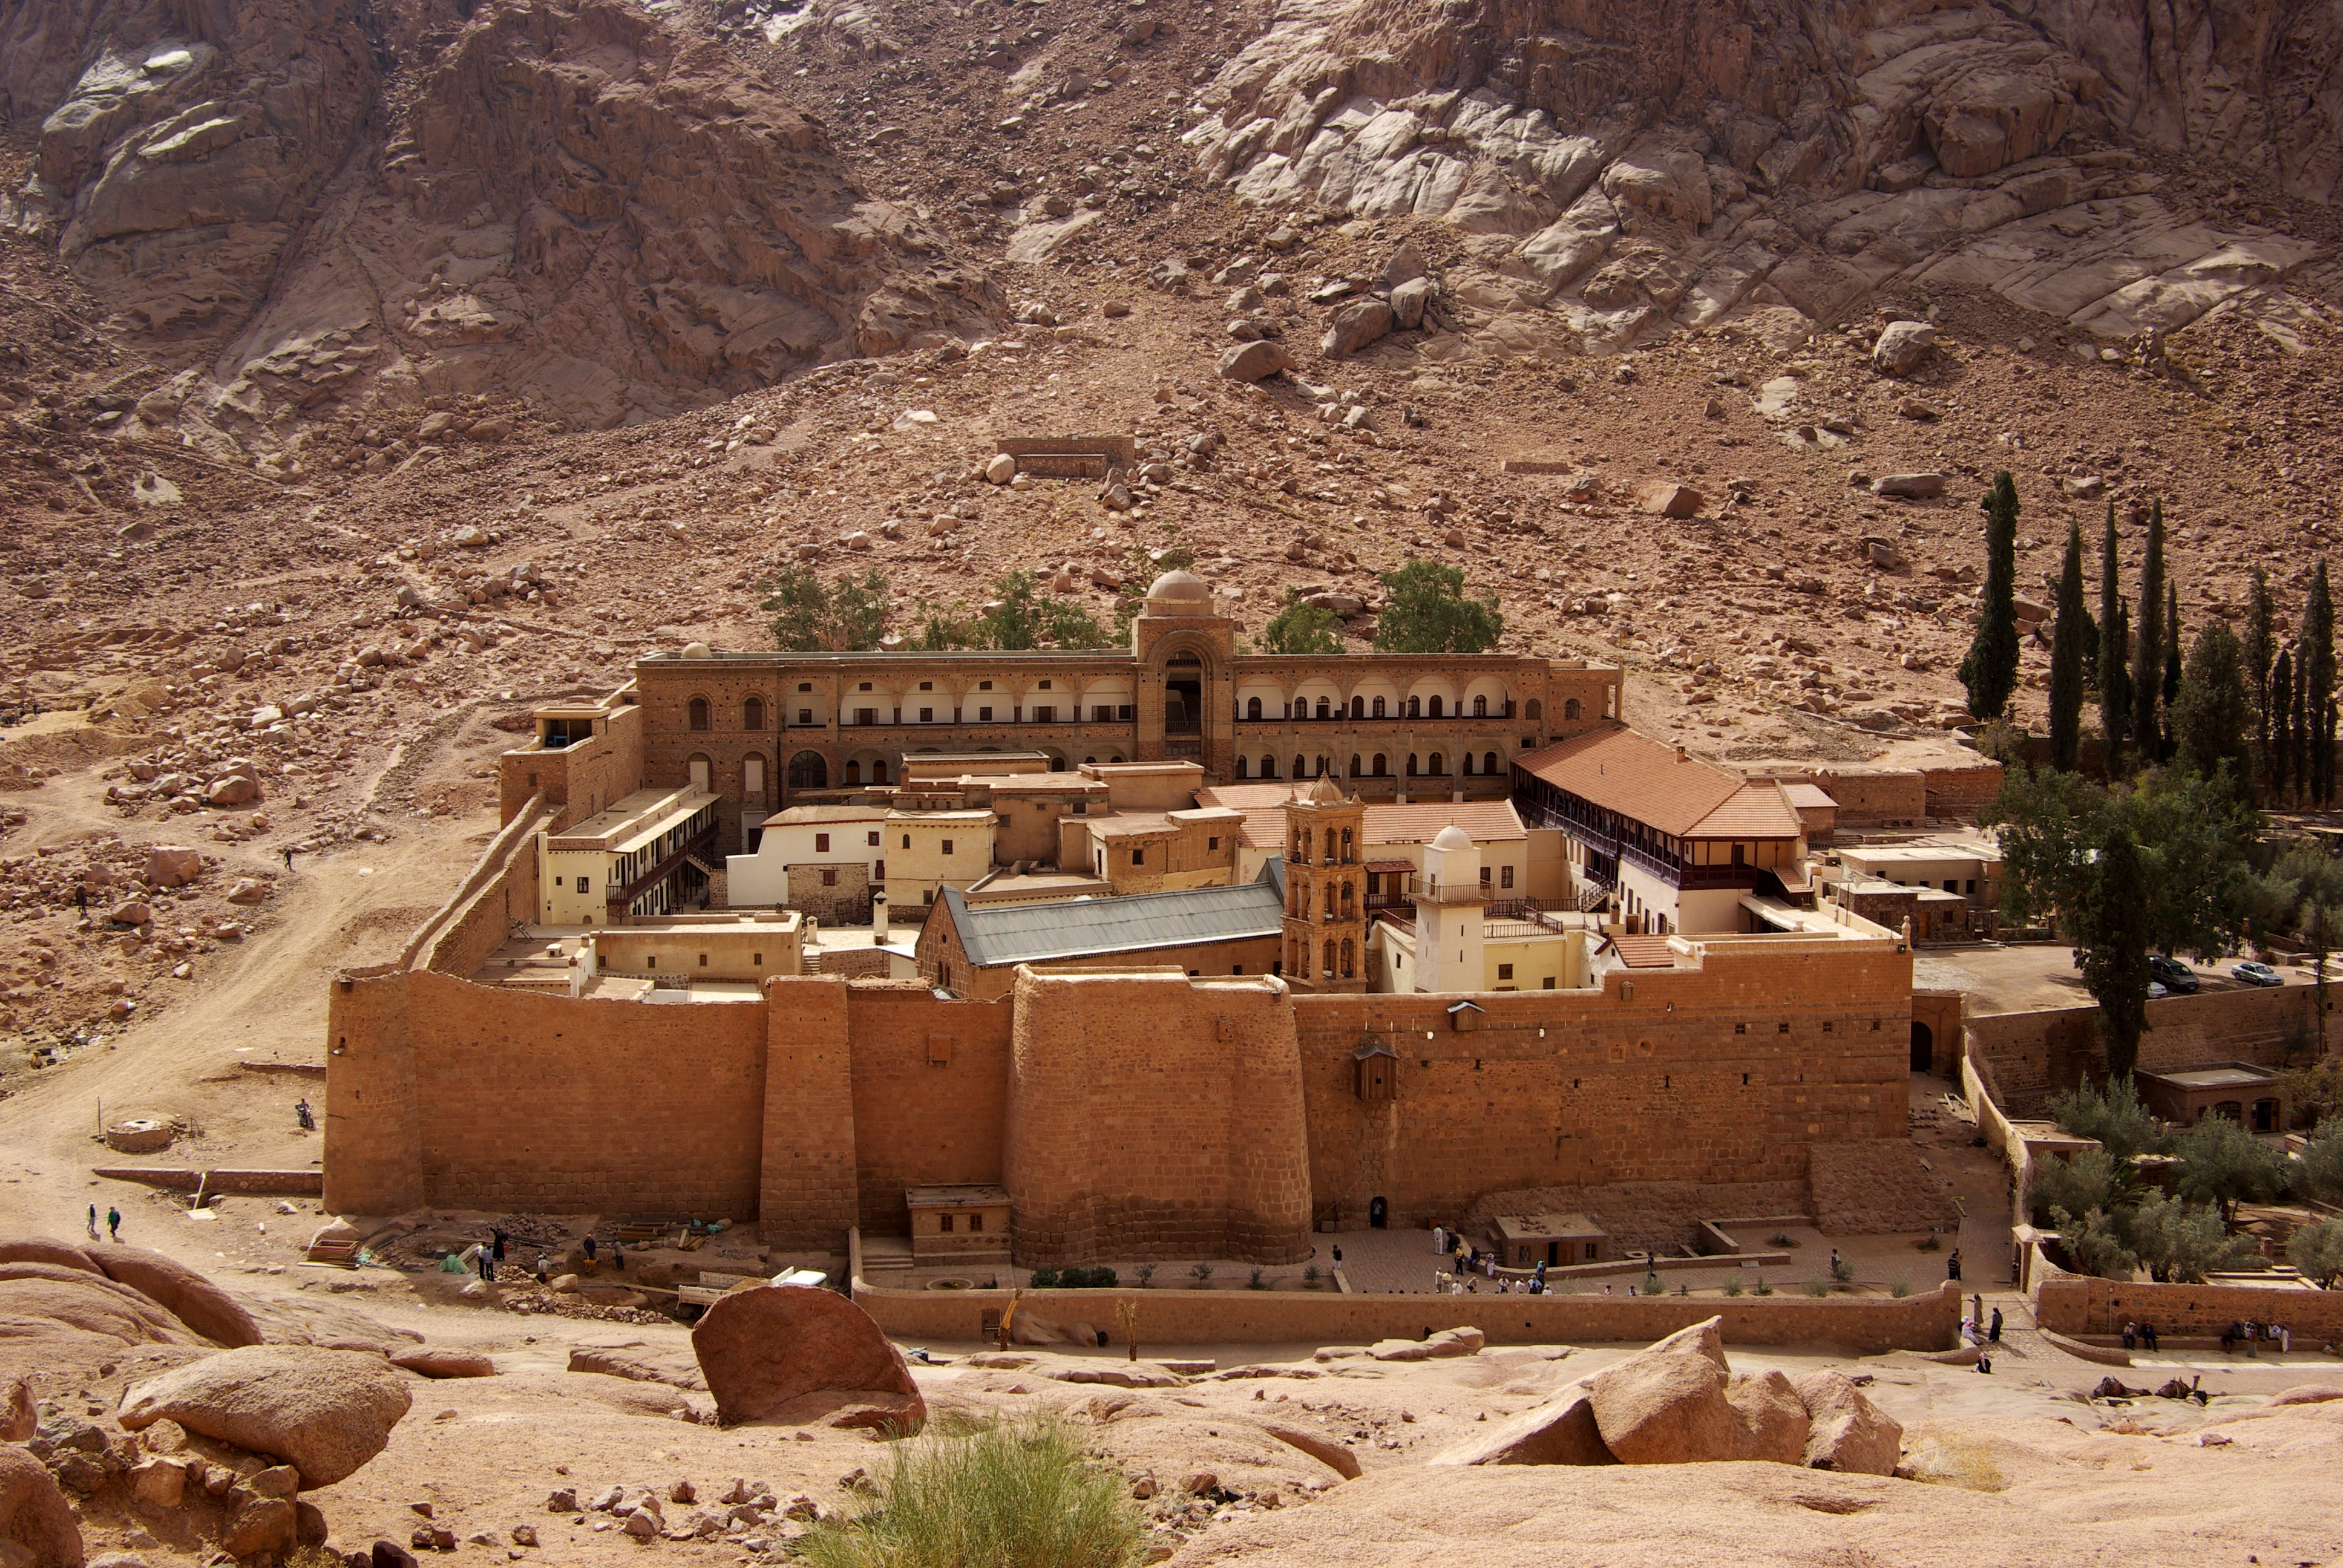
\includegraphics[width=0.5\linewidth]{images/SCP-001-gods-blind-spot.jpg}
    \caption*{\bb{T设施}}
\end{figure}

\bb{描述:}SCP-001是一不规则形状空间,面积约65000平方米,包括地上和地下两部分,位于西奈山███████。除了其奇术性质(见下),SCP-001没有特殊之处,物质与能量可以自由出入其中。法国科学与艺术委员会在18世纪后期进行的考古研究表明此地有一石头建筑,可追溯到公元前2000年,类型符合住宿旅馆。由于T设施的建造,此原本建筑遗迹已无留存。

SCP-001的特殊之处,在于其为目前地球上已知唯一一处天然的Akiva辐射绝对零环境。实验已证实即便将Akiva辐射源引入SCP-001空间范围\footnote{参见研究报告SCP-001.08.P(佛陀齿遗物),1974。}的周围或内部此情况仍会维持,这表明并不仅是SCP-001的外边界严密阻隔了Akiva辐射穿过,SCP-001本身也在吸收和消灭发生于其内部的Akiva辐射。

作为SCP-001性质的结果,智人对象认知功能与器官功能的自然劣化、终结过程会在对象身处SCP-001边界内时中止。换句话说,在特定条件下,人类不会在SCP-001中死亡。参见下列测试记录:

\begin{longtable}{m{0.15\linewidth}m{0.6\linewidth}m{0.15\linewidth}}
\hline
\multicolumn{1}{c}{测试} & \multicolumn{1}{c}{参数} & \multicolumn{1}{c}{结果}\\
\hline
\endhead
\hline\multicolumn{3}{r}{\small{接下页}}
\endfoot
\hline
\endlastfoot
01.001 & 人员D-1082,健康人类男性,安置在SCP-001内部的标准收容间内,观察120天。 & 无变化。\\
01.003 & 人员D-2326,健康的人类女性,安置在SCP-001内部一气闭容器内。向容器内注入致命剂量氰化物气体,测试完成后将气体排出。 & D-2326未出现有害医疗问题。\\
01.006 & 参数同于测试01.003,但对象为30只健康的大白鼠(\ii{Rattus norvegicus})。 & 对象死于氰化物中毒。变体测试表明SCP-001的维生效应仅限于人类对象。\\
01.009 & 人员D-5337,患有4阶段癌症的人类女性(转移到大部分器官),预后其将立即死亡,将其安置在SCP-001内标准收容间中,观察786天。 & 无变化,身处SCP-001内期间对象的癌症症状无任何恶化。对象在测试结束离开SCP-001后的48小时内死亡。\\
01.010 & 人员D-5361,健康人类男性,将其安置在SCP-001内的焚化炉中然后启动。 & D-5361的身体如正常受控程序一样燃烧。其残骸没有特别之处。变体测试表明SCP-001的维生效应没有包括到全部类型的伤害。\\
01.338 & 人员D-8874,健康人类女性,安置在标准SCP-001内标准人形收容间中并被束缚。将对象的左腿在无麻醉下于大腿处截断,且不使用麻醉或止血带等束缚股动脉的措施。在截肢后,其断腿被移出SCP-001,对人员D-8874进行360天的观察。 & 对象暂时失去意识(可能是由于疼痛及突然失血)但恢复,流血在12小时内停止。截肢处快速愈合。移出SCP-001的断腿正常分解腐烂。\\
01.537 & 人员D-13926与D-13927,健康人类男性双胞胎,年龄24岁。D-13926安置于SCP-001内的标准长期人形收容间,D-13927安置在其他基金会设施的长期人形收容间。对象被观察26年零10月。 & 人员D-13927表现出正常的生理变化进程,而D-13926在测试期间没有出现明显衰老。测试结束后D-13926被送往其他基金会设施,这之后对象出现了加速发生的衰老变化。
\end{longtable}

已在T-01号楼内建造了居住设施,可供基金会O5议会全体成员和其他高级管理人员生活居住。当前,12名O5议会成员中有9人居于此宿舍内,此9人中的8人自T-01号楼建造完成起便再未离开。\footnote{第九位O5成员离开T-01号楼处理个人事务,在预定返回前遭气象事件杀死。}

因SCP-001的性质,其也被用作基金会奇术研究计划的控制站点,包括\hyperref[chap:SCP-2336]{SCP-2336-A个体}的应用开发。

\bb{归档文件06-S7INF-23-A(摘录)}

\begin{figure}[H]
    \centering
    \includegraphics[width=0.5\linewidth]{images/SCP-001-gods-blind-spot-2.jpg}
    \caption*{\bb{手稿“对上帝实质的观察”(艾萨克·牛顿爵士)基金会收藏品。}}
\end{figure}

\begin{scpbox}

…在自然哲学和对全能上帝本质的问题上,我们必须凭着感官的证据开展探究,包括神圣经文的证词。虽然无人曾见得上帝,然而对上帝之感知可来自观察他的创造,及至对神圣经文的细致研究。

思考出埃及记第四章,以希伯来文写是:

\usefreeserif{ויהי בדרך במלון ויפגשהו יהוה ויבקש המיתו׃}

\usefreeserif{ותקח צפרה צר ותכרת את־ערלת בנה ותגע לרגליו ותאמר כי חתן־דמים אתה לי׃}

这,将其翻译,是说:

\ii{摩西在路上住宿的地方,耶和华遇见他,想要杀他。西坡拉就拿一块火石,割下他儿子的阳皮,丢在摩西脚前,说:“你真是我的血郎了。”}\footnote{出埃及记4:24–26}

思考这些诗篇的教导。许多饱学学者将关注点投于诗篇第二段,这里西坡拉,摩西之妻,施行割礼,且,以此做法,解救她的丈夫免于全能上帝的怒火。在此,学者们说,是一种道德教诲,告诉说没有人,即便是上帝的先知,得以豁免于他的约法。

但思考诗篇第一段,对此了解甚少。全能上帝,已经产生意图杀死摩西,试图如此却失败。这一段是理解上帝本质的关键。我们必须明白若经文是绝对可靠的,且经文在告诉我们全能上帝试图杀死摩西而未成,那么绝对可靠的经文就是在说上帝不是全能的,或至少说上帝的权柄延伸不到这片特定区域。

\bb{艾萨克·牛顿爵士,《对上帝实质的观察》(1734年)}

\end{scpbox}

\hr

\begin{figure}[H]
    \centering
    \includegraphics[width=0.5\linewidth]{images/SCP-001-gods-blind-spot-3.jpg}
    \caption*{\bb{便携式奇术仪器实验}}
\end{figure}

\begin{scpbox}

“…新近发明的奇术设备让我们的教团得以验证长期以来的怀疑,也即神恩-或者以我们某些兄弟更常用的称谓-奇术力–是一种真实的、可度量的实质现象。我的一位同事提出以“akiva”作为此现象的度量单位,来自某些死去很久的希伯来殉道者。这种哲学与技术突破激起了许多计划的启动,包括对全球akiva状况及变化的测绘。这可不是测绘尼罗河源、或是给无聊海岩命名那样的简单事-这份奇术地图将成为价值无量的工具,让我们的教团能利用神恩之力。

“于是,我们组织了制图队,每人配备一台奇术设备,来完成测绘计划,对值得特别关注的地区尤为注意。

“在圣地的某一角,拿破仑·波拿巴为我们指路了。如你们所知,拿破仑1798年在埃及的战役中有法国科学与艺术委员会参与,它们完成了对此国家的全面测量。\footnote{\ii{Description de l'Égypte, ou Recueil des observations et des recherches qui ont été faites en Égypte pendant l'expédition de l'armée française}}报告的第11卷中测绘了历史地点的地理方位,包括圣经中的何烈山。由此,在这份情报的鼓动下,一队共济会及我们秘教团成员,由我带领,动身去往西奈山,重走摩西从何烈山回到法老宫廷的征途。

今夜,我很高兴地报告教团的努力有了成果。我们找到了‘路上住宿的地方’。”

\bb{布拉姆·史托克}\footnote{译注:爱尔兰作家,著名作品是吸血鬼小说《德古拉》;对超自然颇有兴趣,和黄金黎明相关人士有密切交往,但没有他本人明确入会的记载。}\bb{,抄录自黄金黎明秘教团会议备忘录(1874)}

\end{scpbox}

\hr

\begin{figure}[H]
    \centering
    \includegraphics[width=0.5\linewidth]{images/SCP-001-gods-blind-spot-4.png}
    \caption*{\bb{威廉·永利·韦斯科特(基金会档案照片)}}
\end{figure}

\begin{scpbox}

\bb{站点主管威廉·永利·韦斯科特}\footnote{韦斯科特合作创立了基金会的前身组织之一。}\footnote{译注:威廉·永利·韦斯科特,共济会成员,黄金黎明会社的创始人之一}\bb{至Samuel Liddell Mathers的备忘录摘录,1916年10月16日}

…在住宿地研究、测试其性质后,结论只有一个。上帝也有盲点,我们找到了它。

不仅是躲避死亡天使,住宿地的性质能为多种奇术工程带来机遇。我们现在知道Akiva背景辐射等级在住宿地内无论如何都是零。这就意味着,既然这是上帝的盲点,任何在其范围内做出的举动都不会有神学上的后果。我非物理学家,但我们的同事尼古拉已经把它描述成了罪恶的法拉第笼。将此地用作中心决策的总部的适宜性-成为我们新教团的主体,显然是再明显不过的了。

\end{scpbox}

(备注:自建立起,基金会伦理委员会便一直设置于T-01号楼。)

\hr

\begin{scpbox}

\bb{马尔文·斯克兰顿博士的笔记,1924年7月31日(摘录)}

…作为我们对SCP-001性质的研究结果,我们现已准备在Site-36这里开展第一次人造Akiva真空屏障实验,我们称之为反胞体。基本上我们要创造的就是另一个SCP-001。今日的测试将是二十余年奇术工程及应用神学的巅峰。Bertrand,我的助理,说的更为直率:我们要造个盒子,然后把上帝从里面扔出去…

…

结果是自然厌恶真空,也厌恶内禀。我们的仪器读数表明当反胞体启动,测试胶囊内的可测量Akiva倒是降到了零,休谟等级却飙升了。我们觉得有其他东西-我们现在还没法观察测量-进来了。我们不知道那是什么或者要去何方…

\end{scpbox}

\hr

\begin{scpbox}

\bb{O5政策备忘K-308(1924年8月2日)(摘录)}

先生们:

自7月31日Site-36的事故以来,异常事件的频率与烈度开始猛烈增高;\footnote{虽然其与反胞体测试的因果关系尚无可信验证,其时间值得注意。}如我们所讨论的,这种情形使基金会必须重修和扩张使命宪章。目前我们已经是一个研究组织。但紧急时刻需要紧急措施,已经有必要让我们的团体不至于收容研究生物了。我们必须迈出步伐,控制尚未被基金会取得的异常,即是为了保证异常不被更多研究,也是为了保护全人类。

基金会在此批准成立活动外勤行动部门,立即生效。现存的研究活动就此改组为包含独立的不同研究部门。在此授权这一新机构部门立即组建、投资、招募、装备、训练与部署一或多支机动特遣队。外勤行动部门的临时领导及预算列于附录展示…

\end{scpbox}

(备注:备忘K-308是基金会不再止步于研究、而是积极收集与收容异常项目、实体与现象的正式开端。)

\hr

\begin{scpbox}

\bb{备忘}

\bb{至:管理员;O5议会}\\
\bb{副本抄送:Muhammad al-Taqi主管(战略神学办公室)}\\
\bb{自:Sheldon Katz先生}\\
\bb{日期:19██年8月3日}

Re: 谈判状况(乌列尔计划)

我相信我们已经与对方达成了理解。本备忘的目的是记录理解之要目。如我们所讨论的,正式合约会以协约的形式呈现。\footnote{预期为石板,但我已要求提供PDF文件。}

\uu{背景}

基金会在T设施的行动已多次成为我们与对方关系的胶着点。而近期的发展,因太过宽泛在此略去,令基金会高层管理寻求与对方达成友好关系,既是为促进持续研究与收容工作,避免加速神学末世灾害发生,也是为维持如\hyperref[chap:SCP-1844]{SCP-1844}收容方案等特定基金会协议之效力。之后在高层管理指示下,我办公室展开了与对方的谈判活动。下文概要之重点为这些谈判的结果。

\uu{理解重点概要}

1. 不得有自然人连续停留于T设施内超过120年时间。此限制适用于O5议会成员、其他基金会管理层及员工、测试对象、以及其他。预期基金会强制实行此限令。

2. 伦理委员会记录备忘录应向对方传达,频率不低于每年一次。\footnote{此通信的具体物流方式尚未确定,但我猜测它将是写在羊皮卷上,之后在T设施外的火盆内烧掉。}

3. 对方不得在没有提前至少90日的书面通知及一次违令补救机会的情况下打下、降下或以其他方式施加愤怒于姓名列于列表A内的基金会人员(随各方共识偶尔修订);但例外是此条款在普适性苦难下不适用。

4. 基金会或其管理执行层人员不得屈服或崇拜除对方外的其他神性实体;因为我,主是忌邪的上帝;恨我的、我必察罚他们的罪愆、从父亲到儿子,到三四代。\footnote{对方坚持加入此条款。因此条款实际不要求行动而仅是禁令,我在考虑后加以接受。我假设此第一人称草案将在最终版中修正。}

5. 基金会及对方将以经济上合理的努力,协作收容列于列表B内的有害实体(统称“安哥拉·曼纽”)。

请在正式合约完成前联系我商讨理解要点。

此致,

\ii{Sheldon Katz,上帝\slash 们\slash 的先知}

\end{scpbox}


\chapter[SCP-001 常态]{
    SCP-001 WJS - Normalcy\\
    SCP-001 常态
}

\label{chap:SCP-001.normalcy}

\begin{whiteboxbb}

\begin{center}

\Gg{O5议会备注}

\end{center}

为免你疑问为何这东西在这不属于它的地方,要记住两件重要的事。

第一,SCP-001位置是专门保留给O5议会在其认为必要时使用。

其二,“共认现实”就是议会的一致共认。

\end{whiteboxbb}

\bb{项目编号:}SCP-001

\bb{项目等级:}非异常

\bb{特殊收容措施:}SCP-001保存于专用服务器或图书馆,地点由O5议会选定。对O5成员接触SCP编号项目的常规禁令不适用于非异常下的SCP-001。

对SCP-001的任何添加、删减或更新都需经由O5议会全体一致决定。仅限O5议会接触SCP-001。其他基金会成员或非基金会实体的接触将构成收容突破,可能导致一次破碎化装舞会情景。批准在发生收容突破时进行全面记忆删除施放,随需要至多包括A级记忆删除。

\bb{描述:}SCP-001是一描述共认现实的文件。异常活动被定义为任何超出文件内参数外的活动。文件可能将特定的现实特征描述为固有性异常,取决于O5议会决议。

通例已包括宇宙重力定律、物理力、基础化学、生物学、社会科学、哲学。当前,新发现与技术进步若是建立在既往编定共认现实的知识框架上,且使用了科学方法,将不被视作异常。所有新宣布的发现将被监控是否存在SCP-001参数外的可复现发展

无法被复现的发现宣言,以及似乎只影响宣言报告人感知的发现不被视作异常,可被允许公开。在大部分情况下这些宣告可能会被公众成为“幻觉”、“奇想怪论”或“阴谋论”,不予重视。鼓励此种情况,当异常被公众广泛目击时可以此作为可信的否定。

所有在SCP-001参数外的活动与项目将被追踪、控制、收容,从公众认知中移除,接受SCP基金会保护。对此类项目的研究可用于未来更新SCP-001的提议。

\begin{center}

\Gg{下列摘录已被O5议会确定为SCP-001更新提议样本。所有案例中提出者不予标注,记录也非完整。}

\end{center}

\begin{scpbox}

\bb{提议日期:}1\slash 11\slash 1932

\bb{更新提议:}将在英国出现的现代魔法仪行宣布为异常

\bb{对话:}

我们为何要掩盖这些?这些是整个历史里的文化传统信念,我们不将其视作异常。我们决不能用自己的地位去威胁人类的信仰权。

除非这不是从传统实践中引申出。这种新的“魔法”是现代发明,作为基督教的替代物发展自对仪行的学术再解读。这不是一种延续,这些实践者在试图施展法术。

很快你们会看到亚雷斯塔·克劳利对此有所作为。文件很清楚:神通属于异常,宗教和灵性不是。给我证据证明他们在施展无法被严谨测试解释的咒语,我会亲自看看如何收容这些咒语。在那之前,不,就如泰勒玛是被允许的,巫术也应是如此。看在上帝的份上,我们会一直允许撒旦教,只要它不去沟通恶魔能量。

同意。此外,我们会需要所能召集的全部信仰去对抗神通传统。我们从来不知道一种新信仰会在何时支援到我们。

\bb{结论:}不予更新

\end{scpbox}

\begin{scpbox}

\bb{提议日期:}16\slash 7\slash 1945

\bb{更新提议:}就核裂变主题重新评估物理学

\bb{对话:}

感谢你们回应我的紧急呼叫。三一已经发生了。我只能理解我所见的。就像太阳从荒漠的沙中升起,毁灭的黎明与蔓延几英里远的烈火。我甚至无法相信此等爆炸会被视作有可能性。传闻和过往召唤神明的证据都没有如此冲击力。我为人类将运用此等力量拨动开关即可夷平一座城市的能力。可能而恐惧战栗。

德国人和俄国人是不是也开发出了这种技术?我们在打仗,这种扩张是会发生。

需要我提醒我尊敬的同事们我们没有在打仗吗?美国、日本,他们在打仗。我们不是国家。不,问题是:这是异常吗?这种物理效应是从数学概念推出的吗?

确实是推导出的。每一步都完全是科学测试后才达成这一点。我不相信这是异常,无论后果是多么可怕。

怎么,我们要让人类手握自己毁灭的钥匙?我们拼命战斗就是为了让这种可能远离人类所能及,你们现在说要我们放弃目标吗?

我们没有预防毁灭。我们隔绝的是异常。只要我们同意测试是经由勤勉的科学过程、对所有人可用-

\ii{对所有人可用}?听听你说的话,伙计!你能想象在未来随便哪个不值钱的独裁者都能随心所欲释放数千个太阳的火焰?也许问题不在于等式。也许整个核物理都是异常。

恩里克·费米已经为他在超铀元素和辐射上的成果赢得诺贝尔奖。我们不能只在世界上控制核物理学。辐射无处不在,要这样把自己送回黑暗时代的话只会引发更多矛盾。试试不用共价键解释化学。试试解释生物学。核物理就在这里,我们最好学会习惯这种节奏,无论这对此星球和人类会多么恐怖。

愿上帝怜悯我们的灵魂。

\bb{结论:}将近期在核裂变上的研究、增添及其释放的结果添加到了SCP-001中。

\end{scpbox}

\begin{scpbox}

\bb{提议日期:}2\slash 4\slash 2014

\bb{更新提议:}分类“蠕虫行者”现象

\bb{对话:}

向不熟悉主题的人解释一下,“蠕虫行者”是一种桥段,指某个角色实际是一群由集体心智的蠕虫聚集在一起。我们在这里不是要讨论这种桥段。而是讨论近期从中产生的阴谋论。这种阴谋论认为某些人实际是能行走的蠕虫,而非人类。

这种阴谋论有任何价值吗?

不。阴谋论支持者自己内部对谁是蠕虫行者而谁不是也存在分歧,而所有证据都表明他们不是在人群中行走的蠕虫。非常明确这是属于不可复现的阴谋论理论。我相信SCP-001没有什么可改变的。

这可能不是如我们认为的那样不可复现。

何出此言?

在12\slash 11\slash 2013,一位相信此阴谋论的阿拉巴马州迪凯特居民杀死了他的邻居,因为相信他的邻居是蠕虫行者。凶手之后从邻居家中拍了视频发布到YouTube,称这就是阴谋论的证据,尸体就在他的面前消解成了一群蠕虫。他说他要去采集样本。视频很快被屏蔽移除,所有看过视频的人都同意对象没有移动或者消解成一堆蠕虫。凶手手握一罐颤蚓向警方自首,邻居被送去摩根县停尸房。尸检确认死者的拇指在死后被移除,死因是胸口被枪击——如果他是蠕虫行者,就应该能活下来。

所以,这只是个疯人的行为而已?不是真的阴谋?

关注点在尸检进行后,一位助理法医监督将尸体送还亲属。这位助理法医也是阴谋论的支持者,虽然此前没有接触过相关内容,他一进入检查间就开始恶心地大叫,拿着一张地图,诉称蠕虫到处都是。没有其他人注意到蠕虫侵害迹象。

我们确认他没有偶然看过视频之类的?

我们还不确定。所以,为进行测试,我们取得了尸体将其给D级人员展示。他们都同意这是人类尸体。我们接着向他们介绍了蠕虫行者阴谋论,在再次观看尸体后,他们中有20\%同意这其实是一群蠕虫。

那么听起来像是一种模因危害。这种阴谋论文本又被CH部门扫描过吗?

CH发现其模因效应为阴性,但发现有一小册内的章节可作为记忆触发点,解锁一段记忆。当然,只有受影响者有这种记忆时才行。

这段记忆是?

最近看到过活体的蠕虫行者。

\bb{结论:}关于记忆触发点的术语被增补以包含近期发现。虽然依旧无证据表明蠕虫行者阴谋论的真实性,然而有效记忆触发点的存在的后果值得思考。总之,你有没有听说过有东西dowwÐÁ“ŒÏMA3§

\end{scpbox}

\tred{更𡖈报告 - 仅限O5查阅}

\tred{访问兀讠午}

\begin{scpbox}

\bb{提议日期:}21\slash 14\slash 211zÔâµ½ž±—4ö0¯žÛ¼’Ýn

\bb{更新提议:}超记叙异常šZؾ‡ƒuÔ5

\end{scpbox}

\begin{center}

\bb{侦测到试图访问SCP-001。身份考验激活。}

\bb{部署模因处决触媒}

\begin{figure}[H]
    \centering
    \includegraphics[width=0.8\linewidth]{images/SCP-001-normalcy.jpg}
    \caption*{由是你非真\protect\footnotemark}
\end{figure}

\footnotetext{图片内容:“现实就是那个,当你不再相信它时,仍然挥之不去的东西”-菲利普·K·迪克(译注:《高堡奇人》作者)}

\end{center}

{[}访问SCP-001]

\begin{scpbox}[hbox, parbox=true, center, unbreakable, before upper=\begin{varwidth}{0.5\linewidth}, after upper=\end{varwidth}]

黑月是否嚎叫?\\

{[}\qquad\qquad\qquad\qquad]\\

\rightline{取消\quad \hyperref[sec:DOC-wjs-proposal-1]{确定}}

\end{scpbox}

\newpage

\section{SCP-001(解锁)}

\label{sec:DOC-wjs-proposal-1}

你好。

我已经在此恭候你了。既然你成功通过了我们的考验,你可能是来自混分的星级前认知骇客,\hyperref[chap:SCP-301]{Argent博士的宠物},或者某种超记叙实体来翻阅我们的数据库供你病态娱乐(是的,我们知道你在那,YOUR-USER-NAME\footnote{\QIS:网页上此处会显示你的用户名}。这也是为你留的。)不管你是谁,你在这里读到这些的事实就意味着一件事:你是异常。

我恐怕你不会在此找到SCP-001。它存放在某个远比这里遥不可及的地点。我肯定你在期望自己能找进去,在这里或那里编辑它一下两下,然后voilà,你就不再是异常了,你就自由了,基金会不会妨碍你了。当然,不可能这么简单。但我会帮你。你应得如此。

我要告诉你\ii{为什么}。

\ii{为什么}基金会瞄准了你。\ii{为什么}我们认为你是要被收容的东西,要被烦扰。毕竟,世上还有更多更坏的邪恶。我们把对核武器的记录放在上面当做示例。历史上有过无数次种族屠杀。光是流感造成的死亡人数,就远超出我们收容的这数千人和物的破坏潜力,然而我们偏偏投身自己来把你标为\ii{异常}。\ii{不正常的}东西。天生\ii{错误}的东西。不能被放任的东西。

为什么?

我不会摆出架子说我无能为力。我只是议会中的一股声音,我不能靠自己改变什么,这是真的,但我所做的决策,还有我让自己看待你境遇的方式,都是人们看你适合被扔进盒里的直接原因。即便我不能改变文件,我也能为你是正常保留一两个支持。毕竟,人类已经相信幽灵鬼魂的存在数千年了。我们都在孩提时相信过床下的怪物。这些现象非常真实,也完全是世界运作的一部分。为何我们不能就宣布它们是\ii{正常}?为何我不让你摆脱折磨?

因为我们不是只在这里控制、收容、保护这世界。我们在这里是控制、收容、保护你。

对异常的定义是其无法被简单的科学测试所揭示。这让你和你的本质有所\ii{不同}。甚至说,是独特。这种稀缺性让它有了价值。这不意味着你的价值是所有人都会欣赏的。有时,只有那些愿意用它反对你的人才会欣赏。

这种稀缺也是怪物得以利用你的工具。其他人不熟知你的异常,不会把对它的描写认为是真的。这给恶毒的人以机会利用这种无知,利用你作为他们取乐的可憎棋子。他们可以孤立你,吞噬你,让你的异常成为他们破坏的工具,用你的存在满足施虐的渴求。

我肯定你见到过这种事情。有人不一样。他们的愿望、需求、他们的现实迫使他们被大多数世界流放。他们被孤立。可能不是没朋友,但也是被边缘化,渴望交流。这时有人上门,允诺甚佳,但给予你所渴望的交流,靠的却是吞噬你,消灭你的世界,曲解你的现实。你反击,想把你的境遇向谁倾诉,但其他人回答,“哦,这不可能发生。这不是真的。你一定是搞错了,”你就独自留在了异常里,独自受苦。

我们不能让此发生。是的,继续,说我们到底也是孤立了你,慢慢吞噬你和你的存在,这和某些虐待狂希望火烧你们一样肯定。称我们是禽兽。没问题。但记住即便我们追捕你,我们掩盖,我们监禁你,我们还是希望保证你继续存在,你不会从世界上被完全抹除。你有权存在。你有权做不同的自己。

你,那个在那里的怪物、在这里的怪物,你同我们一样完全真实。和这遍布、鲁莽、自我毁灭的人类一样,与这对你境遇一无所知的人类一样真实。结论是,我们到头来都是一路货色,我希望你在这里找到些宽适。

是的,你是个怪物。但,无论我们是否认定异常,我们中的最后一员也会如此。这意味的是你值得存在。

我们控制你。

我们收容你。

我们保护你。

即便你还是不理解为何我要这么做,也请理解我依然爱你。

\ii{- O5-5}



\chapter[SCP-001 世界,收容失败]{
    SCP-001 BILLITH - The World at Large \\
    SCP-001 世界,收容失败
}

\label{chap:SCP-001.the.world.at.large}

\begin{scpbox}

\begin{center}

\Gg{\bb{\mono{您正在访问SITE-01归档文件}}}

\mono{深层存储}

\ii{\mono{请稍候……}}

\end{center}

\end{scpbox}

\begin{scpbox}

\ii{\mono{001.SCP.archive @ dir\slash arc\slash events\slash other\slash EE00059.rtf 加载中…}}

\mono{\bu{事件:}\uu{EE-00059}}

\bi{因EE-00059的性质,无须将其指定为一个SCP。EE-00059存在的情报基本上被认为是非异常的,因此目前不需要制定收容措施。在EE-00059附近发生的任何信号播送和活动都应上报并尽可能从公众知识中清除。}

\bb{事件描述:}2016年1月4日,在距地球约160万光年的太空区域观测到超常事件00059。\footnote{这表明其初始起源距今约160万年。}NASA的深空网络卫星系统在三小时内检测到了它。

EE-00059-1是事件期间的一系列低频传输信号,来自EE-00059方向。考虑到无线电波的范围和速度,其很可能由异常广播设备发送以传输消息。(查阅\bb{EE-00059-1转录日志}以获取更多信息。)

EE-00059-2是一个新出现的E级“因果暂失”虫洞(S-CSMWAUC2-T)。\footnote{空间性,循环稳定,有形体,广域,非定性,条件双向,瞬态。更多信息请参阅:\ii{\hyperref[sec:DOC-about.black.hole]{统一技术设定论述,关于超维度出入口(即虫洞)的分级}}和其他\hyperref[chap:SCP-3989]{类似案例文件}。}EE-00059-2在EE-00059-1-3传输期间被观测到出现约102秒,同时表现出虫洞和白洞的性质,并喷射物质和光线,但对地球上常见的流体流动却有极大限制。这导致其异常可见度比普通情况大了几个数量级。在近距观察后,发现EE-00059-2并未表现出对周围重力有明显影响。这点与埃利斯虫洞更为符合,它是时空的非平坦三维区域之间的完全可转移点。

这种矛盾的表现意味着EE-00059-2是以我们自己的现实中不可能的手段创造的,该区域需要基金会进一步调查。

\end{scpbox}

\hr

\begin{scpbox}

\ii{\mono{00059.SCP.archive @ dir\slash arc\slash events\slash other\slash EE00059_Exploration.rtf 加载中…}}

\end{scpbox}

\begin{scpbox}
    
\begin{figure}[H]
    \centering
    \includegraphics[width=0.5\linewidth]{images/SCP-001-the-world-at-large.jpg}
    \caption*{Altruist-9探测器,位于Site-88航空航天机库。}
\end{figure}

\bi{\mono{2027年5月18日,基金会提议建造Altruist-9深空探测器,以观察EE-00059所在区域的状况,O5议会以多数票通过。}}

为了在一定时间内到达指定地点,Altruist-9采用了超光速(FTL)驱动器和高效太阳帆。但是,由于灵敏度和探测器遭遇外空间异物的风险,超光速驱动引擎不会全功率工作。因此,Altruist-9预计在████年走完全程。

在EE-00059-2重现事件中,Altruist-9存放着一架小型太阳能无人机和一台大气测量设备的内核,被包裹在了一个外源的多肽低聚物编织结构中,物质来自\mono{{[}数据删除,见下]}的残骸。该物质推定是穿过EE-00059-2后存留了下来。Altruist-9于2038年1月8日发射。

\bb{更新:}

████年2月26日,即Altruist-9到达指定位置的时间,记录到的读数在开始是非异常的。然而,不久之后,就检测到了区域内的活动。EE-00059-2似乎在探测器附近重新打开了,并将探测器吸了进去。异常在102秒后关闭。

因白洞的反常和极端性质,Altruist-9可能无法在与EE-00059-2的接触中幸存。但推测探测器内核的功能性应该在穿越中保存了下来,并能够在EE-00059-2的另一侧进行观测,直到未来某天链接重建起来。

\end{scpbox}

\hr

\begin{scpbox}

\bi{\mono{001.SCP.archive @ dir\slash arc\slash events\slash other\slash EE00059-01_Log.rtf 加载中…}}

\tred{+ 访问00059-1-1转录日志}

\tred{确认}

00059-1-1转录日志

\ii{注意:这是从EE-00059方向接到的首次信号传输,持续了30分钟。上下文未知,只听到单方面讲话,标记为POI-00059-A。所有的传输信号使用的都是一种句法结构与英语类似的语言,因此可以相对容易地翻译。}

\hr

<开始转录>

\bb{POI-00059-A:} {[}静电噪声] -未知,也许他们能- {[}静电噪声]

\bb{POI-00059-A:} {[}静电噪声] -去,它不会落在后面太远。 

\bb{POI-00059-A:} 不,我不- {[}静电噪声]

\bb{POI-00059-A:} {[}静电噪声] -我们把它丢了。不确定。

\bb{POI-00059-A:} {[}无法拼出]

\bb{POI-00059-A:} 什么?十,三。是- {[}静电噪声]

\bb{POI-00059-A:} {[}静电噪声]

\bb{POI-00059-A:} 噢。噢不。

<转录结束>

\tred{+ 访问00059-1-2转录日志}

\tred{确认}

00059-1-2转录日志

\ii{注意:记录下的对话持续5分钟,应该发生于两方之间,标记为POI-00059-A和POI-00059-B。上下文未知。}

\hr

<开始转录>

\bb{POI-00059-A:} {[}静电噪声]

\bb{POI-00059-B:} {[}静电噪声]很匆忙,还是不知道什么时候- {[}静电噪声] -我们。

\bb{POI-00059-A:} 不需- {[}静电噪声] -那。我们的传感器正监测到反常{[}无法拼出]。

\bb{POI-00059-B:} 我们也是。你觉得这是- {[}静电噪声]

\bb{POI-00059-B:} 最好别深究。

\bb{POI-00059-B:} 收到了吗?十二,四。

\bb{POI-00059-A:}  只有- {[}静电噪声] -我们现在落单了。

\bb{POI-00059-B:} 那会多久?

\bb{POI-00059-A:} {[}静电噪声] -什么方法找到我们。

\bb{POI-00059-B:} {[}无法拼出]

<转录结束>

\tred{+ 访问00059-1-3转录日志(需00059或4级权限许可)}

\tred{确认}

00059-1-3转录日志

\ii{注意:这是EE-00059-2首次观测期间,从EE-00059方向收到的最后一段对话记录。此次对话持续10分钟,发生于两方之间,标记为POI-00059-A和POI-00059-B。}

\hr

<开始转录>

\bb{POI-00059-A:} {[}静电噪声] -一,四- {[}静电噪声] -一,八,收到请回复。

\bb{POI-00059-B:} 收到,你们需要离开。立刻。

\bb{POI-00059-A:} {[}静电噪声] -跳跃,二十- {[}静电噪声] -重复,二十秒差距。无法- {[}静电噪声] 十五。恒星体依然- {[}静电噪声]

\bb{POI-00059-B:} {[}静电噪声] -得马上离开这,马上!

\bb{POI-00059-A:} 等等,我们发现了- {[}静电噪声]

\bb{POI-00059-A:} 你们能听到吗,我们- {[}静电噪声]

\bb{POI-00059-B:} 是的,我们看到了。接着怎么办?

\bb{POI-00059-A:} {[}无法拼出]

\bb{POI-00059-B:} {[}静电噪声] -太草率了,很可能承受不住- {[}静电噪声]

\bb{POI-00059-A:} {[}静电噪声] -抱歉,Graham。{[}静电噪声] -驱动引擎没法及时就绪了。我觉得这是我们唯一的选择,否则我们必死无疑。

\bb{POI-00059-A:} {[}未知] -靠近了。告诉- {[}静电噪声] -他们。

\bb{POI-00059-B:} 一路平安。

\bb{POI-00059-A:} {[}静电噪声]这。好的我们几乎- {[}静电噪声]

\bb{POI-00059-B:} 什么?你们看见了什么?

\bb{POI-00059-A:} {[}无法拼出]

\bb{POI-00059-B:} 鹦鹉螺号,请重复。二十,四。

\bb{POI-00059-A:} {[}尖叫]

\bb{POI-00059-B:} {[}静电噪声] -螺号!我们得移动- {[}静电噪声] -也许损失- {[}静电噪声]

\bb{POI-00059-B:} 那东西消失了。它去哪儿了?在哪 -{[}静电噪声]

\bb{POI-00059-B:} {[}静电噪声]

\bb{POI-00059-B:} 这里是天命号舰长Graham Ereshkigal,隶属人类████████星系运输船队。如果有人收到,这是我们的最后讯息,地球它,它不见了。我们不确定及时- {[}静电噪声] -能否。我们在Laniakia,或许- {[}静电噪声] -救援,我不知道。我不知道。

\bb{POI-00059-B:} 我们必须进入超光速,但告诉- {[}无法拼出] 

\bb{POI-00059-B:} {[}静电噪声]

<转录结束>

\end{scpbox}

\hr

\begin{scpbox}

\bi{\mono{05.001.SCP.archive @ dir\slash arc\slash mainlist\slash SCP-001.rtf 加载中…}}

\end{scpbox}

\begin{scpbox}

\begin{figure}[H]
    \centering
    \includegraphics[width=0.5\linewidth]{images/SCP-001-the-world-at-large-2.jpg}
    \caption*{SCP-001}
\end{figure}

\bb{项目编号:}SCP-001

\bb{项目等级:}Netzach 

\bb{特殊收容措施:}N\slash A

\bb{描述:}SCP-001是所谓地球的行星体的名称。鉴于SCP-001养育了人类的整个文明,与基金会深空计划所观察到的视界宇宙内其他行星相比,地球的异常不可能性被公众广泛认为是“正常”的。

SCP-001-E1是1956年在智利安托法加斯塔地区阿塔卡马沙漠进行考古探险时发现的航天器残骸的名称,看上去已经被改造为临时生存空间。飞船的残余部分由外源的未知组分高耐久合金构成,材料的年代测定结果也不一致。尽管如此,回收到的材料表明飞船已有数百万年历史。

衣物,电子产品和家具等物品的残余也已收回,所有物品都含有不同程度抗正常磨损的异常材料。飞船的全尺寸未知但据信足够大以能容纳中等数量的人类,除了从SCP-001-E2内部回收的POI-001外,其余残留物均已自然分解。

SCP-001-E2是一组\dd{32} 36个高度先进的低温休眠舱,是挖掘SCP-001-E2时,于一块以部分“冬眠”模式供能的残骸中发现的。在所有发现的舱室中,只有一个仍然在运作并且含有\mono{{[}应监督者要求删除]},该生命体的宗旨使得基金会之后在地球上建立起来。

\end{scpbox}

\begin{figure}[H]
    \centering
    \includegraphics[width=0.5\linewidth]{images/SCP-001-the-world-at-large-3.jpg}
    \caption*{残骸从智利西海岸运离,1957年。}
\end{figure}

\begin{scpbox}

在瓦砾中有几个完全损毁的数据存储设备,目前唯一恢复出的信息片段是一张1cm x 1cm的磁盘碎片,由异常材料构成。已知该材料是一种高度压缩的多层信息介质,呈现为一组垂直堆叠数据的薄层结构。下面是从数据中恢复出的文档,由他们的原始语言翻译而来,这是一组I类认知危害型文字,其性质使得尽管对该语言的理解和阅读水平都很有限,读者仍然能够100%理解材料。对语言的分析正在进行中。

\hr

\tred{访问 001-E1-a89.rtf }

\tred{- 关闭}

\mono{\bb{修订版本:A.89}}

\mono{\bb{分类:神经学}}

\mono{\bb{详情:当前认为A.89行为复合体的实施方案很成功,不需要进一步改动。如果未来出现VIII级大气危害情景,将立即修改和实施A.89策略,以最大限度地减少伤亡并将新的人形生命形式纳入适当的宿主环境。}}

\mono{\bb{A.89行为复合体于124.5, 8.4M实施,在类地的陆地行星AXIOM-8上成功进行了宿主整合。}}

\mono{\bb{在主地球被太阳撞击破坏后的人口迁移行动中,AXIOM-8被认为最适合人形生命生存。已接触AXIOM-8并证实其无人居住并含有氮为主的大气。}}

\mono{\bb{由于VIII类大气危害情景中AXIOM-8被大约21%体积的高腐蚀性O\textsubscript{2}污染,基础设施和人类收容\slash 生活区域的建立进程中断,并且其对大多数生命形式有致命危害,需要实施A.89。}}

\mono{\bb{A.89是一套条件反射和对基础生理学的修改,使用泛星系基金会的\hyperref[chap:SCP-2000]{生物进化诱导器}(BECM)改变了产生的新生命形式的一般生物学特性。A.89的主要复合体是一种下意识的振荡行为,包括短时间吸​​入空气,随后扩张鼓膜,合理平衡周围环境的超压力,并缓解大气中小规模的氮流失及氧的暂时性危险失衡。此外,也正在进行小幅改造,以使得氧气能够成为支持广泛生命的物质。研究正进行中。}}

\mono{\bb{附录:实验记录}}

\mono{\bi{以下为使用泛星系基金会生物进化诱导器(BECM)对应用A.89的生命形式进行各种测试的简要总结。}}

\begin{longtable}{m{0.2\linewidth}m{0.2\linewidth}m{0.5\linewidth}}
\hline
测试编号 & 生命形式 & 结果\\
\hline
\endhead
\hline\multicolumn{3}{r}{\small{接下页}}
\endfoot
\hline
\endlastfoot
A.89-1 & 主地球爬行动物(小) & 应用失败。暴露于AXIOM-8会导致由于压力变化和细胞快速氧化发生的大出血。\\
A.89-2 & 主地球爬行动物(小) & 应用失败。当试图利用新的生理学改变时,受试体死于癫痫发作。为了完善该点需重新调整神经连接通路。\\
A.89-8 & 主地球爬行动物(大) & 应用部分成功。受试体在暴露于AXIOM-8两个周期后才死于细胞氧化,比平时更长。A.89行为似乎可以防止氮剥夺;进行了脂质测量,结果正常。\\
A.89-15 & 主地球爬行动物(大) & 应用部分成功。暴露未导致压力失衡,整个过程中都出现了A.89行为。由于氮剥夺,试体不久后陷入昏迷。\\
A.89-22 & 主地球爬行动物(大) & 应用部分成功。生理适应性失控。受试体表现出抗处决性,在受到损伤后通常以惊人速度恢复。受试体目前关押于高安全收容室留待进一步研究。\\
A.89-27 & 标准人类 & 应用成功。受试体能够承受AXIOM-8的大气。观察到轻微头痛和偶发鼻出血。\\
A.89-38 & 五(5)标准人类 & 应用部分成功。除非聚在一起,否则受试体能够承受AXIOM-8大气。当存在多种生命形式时,特别高密度的氧气仍会导致氮剥夺。\\
A.89-40 & 五(5)标准人类 & 应用部分成功。在群体中施用轻度认知影响以启动A.89可显着降低死亡率。对正在进行的氮气总量要求进行了基础修改,但这些计划在12个周期以后才会完成。\\
A.89-44 & 五(5)标准人类 & 应用成功。97.8%的个体通过认知效应成功避免死亡。正在努力将人类的平均寿命延长回至███。\\
A.89-68 & 一标准人类 & 应用部分成功。细胞氧化扼制足以使平均寿命延长至██,是之前平均值的五倍。对生理学的进一步改造不会有额外增益。
\end{longtable}

\tred{访问 001-E1-axiom.rtf}

\tred{- 关闭}

\mono{\bu{AXIOM-8}}

\mono{\bb{毫无疑问,人体是一个难解之谜。经过数千年的休眠,对新家园的上下求索将我们最终引向了一个与主地球有着惊人相似之处的星球。这是最大的谜团。}}

{[}数据损坏]

\tred{访问 001-E1-note.rtf}

\tred{- 关闭}

{[}数据损坏]

\mono{\bb{能经得起时间的考验,如果你发现了它,而我们已不再存在,或者我们忘记了我们是谁,我们来自哪里,那你应该知道我们的过去,人类,是命运之子。}}

\mono{\bb{我们\ii{会}活下来。无论发生什么。}}

\mono{\bb{正如}}

{[}数据损坏]

\mono{\hyperref[chap:]{所以我们要坚持下去}。}

\hr

\end{scpbox}

\newpage

\section{统一技术设定论述,关于超维度出入口(即虫洞)}

\label{sec:DOC-about.black.hole}

\tred{+ 查看不必要的科学文献}

\tred{– hide block}

\GG{\tred{统一技术设定论述,关于超维度出入口(即虫洞)的分级}}

\hr

\bb{目的:}量化并整体上把超维度出入口理论联系起来,基于实际使用和作品情况指派相应的名称,为基金会写作带来方便,也为作者们提供一个量子叠加态方面的设定。\footnote{也就是说,它既\ii{是}设定,也\ii{不}是设定。}

\bb{简介:}本质上,我想提出一个参考系统,能把当前出现过的超维度出入口松散地联系起来,或者帮助更好地理解它们。本篇论述将解释名称,并适时举例说明。我会尝试对每一个写入过数据库的虫洞进行分类,并在此套系统下根据它们传输物质的效率,收容方面起的作用(参照斯克兰顿现实稳定锚),以及其他附属任务进行分级。

\ii{作者注:本文档使用了几个已建立的基金会宇宙伪设定,如果写手赞同的话,可以直接用到作品中。这些名称大多都是纯理论假设的,所以可以更改。}

\hr

\Gg{\bb{A级:}“相对论完整性”虫洞}

A级虫洞很适合基金会传送工作使用。它在折叠时空方面涉及的理论领域完全可以使用标准相对论物理模型描述。

这种虫洞包括自然出现的虫洞,其内部量子场可以被稳定在一定数值以允许以太自由流动。同样地,那些对基金会行动机动性有极大帮助的异常区域也可以归到其中。

A级虫洞示例:

\begin{itemize}
\item \hyperref[chap:SCP-1322]{SCP-1322}\footnote{如果它能被基金会完全控制的话;据我所知,目前没有Thaumiel等级虫洞存在(适时而变)。}
\item \hyperref[chap:SCP-120]{SCP-120}
\end{itemize}

\Gg{\bb{B级:}“信息高速路”虫洞"}

B级虫洞可以让物质以存储的信息方式运输\footnote{一般来说,这意味着B级虫洞是自然形成的。该过程通过“超填”量子储存塔到大于10\textsuperscript{69}bits\slash m\textsuperscript{2}的密度完成,其将使得媒介物坍缩为一个黑洞,并可通过后期修改来实现数据到数字或模拟现实的转换。更多信息请参见\hyperref[chap:]{信息是基础的吗?}。}。该过程可用于创建有形的网络接口,以实现数据的物理交互,与已构建地点之间的传输。

B级虫洞示例:

\begin{itemize}
\item \hyperref[chap:SCP-1549]{SCP-1549}中有提及
\end{itemize}

\Gg{\bb{C级:}“破碎入口”虫洞"}

此类虫洞为一不稳定的时空折叠,无法将物质传送到指定位置。在其出现\footnote{一种人为时空操纵的可能后果,因为理论认为虚无维度是两个不相关维度上的点在发生超维重叠时时空为抵消其不可能性而产生的自平衡现象。}时会产生小的虚无维度空泡,如控制不当可能会产生危害。这些虫洞无法预测,会喷射出未知来源的物质。

C级虫洞示例:

\begin{itemize}
\item \hyperref[chap:SCP-3001]{SCP-3001}中有提及
\end{itemize}

\Gg{\bb{D级:}“非回溯”虫洞"}

D级虫洞是基础的销毁单元,其通向非宇宙。它们是时空曲率的标量恒定处,指空间中不存在现实与物理定律的点。\footnote{这到底会形成一个黑洞还是使得此虫洞消失还有待观察。}

D级虫洞示例:

\begin{itemize}
\item \hyperref[chap:SCP-123]{SCP-123}
\end{itemize}

\Gg{\bb{E级:}“因果暂失”虫洞"}

E级虫洞定义了许多不可能存在的超维区域,因此对现实存在有异常影响,或者无法以对基金会有意义的方式创建利用。它们要么已经消失,只是昙花一现且没有明显的(也可能是异常的)原因,要么以违反自然法则的方式存在。通常,这些出入口是在固定位置由异常手段创建的,并且对基金会的行动没有任何益处,甚至需要进行分级和收容。

E级虫洞示例:

\begin{itemize}
\item \hyperref[chap:SCP-3321]{SCP-3321}
\item \hyperref[chap:SCP-3221]{SCP-3221}
\item \hyperref[chap:SCP-1437]{SCP-1437}
\item \hyperref[chap:SCP-2510]{SCP-2510}
\end{itemize}

还有更多,我敢肯定。

\GG{\tred{为什么?}}

这是个大问题,是吧?为什么这个?为什么那个?为什么笔耕不辍?为什么搞出了休谟?

我喜欢我虚无的格式塔组织有统一的术语。那能让我觉得心中很快乐,也巩固了基金会的临床腔结构。

但大家还是要记得:

\ii{“没有什么设定。”}



\chapter[SCP-001 死人]{
    SCP-001 Tanhony - Dead Men\\
    SCP-001 死人
}

\label{chap:SCP-001.dead.men}

\begin{scpbox}

\grey{\mono{你好。我是希腊化.aic,基金会监督者的档案通讯专用2.0版人工智能应征员。今日我要如何帮助您?}}

\end{scpbox}

\blue{输入:访问5级文件网络}

\begin{scpbox}

\grey{\mono{访问申请的网络中…}}

\end{scpbox}

\begin{scpbox}

\grey{\mono{一些备注:网络仅限}}\mono{\red{O5议会}\grey{和处理SCP-001的研究员访问。需要通过验证。未能通过验证时将出动MTF-Alpha 1(“红右手”)。您希望继续吗?}}

\end{scpbox}

\blue{输入:继续。}

\begin{scpbox}

\grey{\mono{黑月是否嚎叫?}}

\end{scpbox}

\blue{输入:地狱的猎犬有三头。}

\begin{scpbox}

\grey{\mono{噢。哦!越权成功,长官!欢迎!已经好一段时间了。}}

\end{scpbox}

\blue{输入:访问SCP-001主文件。}

\begin{scpbox}

\grey{\mono{当然!正在打开申请的文件…}}

\end{scpbox}

\bb{项目编号:}SCP-001

\bb{项目等级:}Thaumiel

\bb{特殊收容措施:}SCP-001收容于\hyperref[chap:GUIDE-secure-facilities-locations]{Site-01}。为避免SCP-001受伤害的风险,任何情况下不得有其他异常项目收容于Site-01。已散布关于O5议会不被允许接触异常项目的掩盖故事,以保密SCP-001的存在。

SCP-001收容于标准人形收容间,由六名安保人员全体看守。SCP-001将配备一支医疗小组全天看护,以快速处置任何突发的健康问题。类似地,一队神经外科医生将在站驻守以应对SCP-001的校准故障。SCP-001意识内的认知触媒将每两日强化一次。

直接处置SCP-001的全体研究人员应精通奇术学和Erikeshan概念工程学。为避免在SCP-001濒临死亡时出现概念缺省回转,将以存储于Site-01的D级人员立即执行协议勒梅-17。

关于已解体GOI-6616(“永恒之环”)的全部信息将从公众及基金会记录中移除,只可在Site-01机密档案库内查阅。

\bb{描述:}SCP-001是一84岁男性,在概念上已与广义的死亡进程相融合。以此,通过SCP-001为触媒,死亡进程本身可在一定限度内被操控。例如,SCP-001在被基金会收容前遭减除舌头、其耳膜也被伤害致残,确信这是为减少在当代出现独家性“死亡交易”的几率\footnote{参见奇术档案库内A.A. Gilford的《消失的魔法:哄骗死亡的侵蚀》获取详情。}。

通过一系列神经外科手术和认知治疗,SCP-001已被成功地置于一种定向\footnote{参见Dr. Harold Gradian的《知觉流变:新千年的记忆删除》}面容失认症中;具体来说,它无法认知任何O5议会成员的面容。因其概念状态,它的这种能力缺失将延展为死亡本身的能力缺失。其结果是所有O5议会成员不可能死亡或衰朽。预定在未来将这一死亡免疫状态扩展给其他关键人员。

确信SCP-001最初是由名为“永恒之环”的伦敦团体使用奇术和Erikeshan概念工程学联合创造。SCP-001及描述其创造过程的记录在对该组织总部的突袭中得以寻获。该组织大部分成员在此次突袭中被杀。在发现SCP-001的潜在用途后,它被送往当前的Site-01地点,编为Thaumiel级异常。

从SCP-001的生理状况和缺乏对刺激的反应来看,确信其在被GOI-6616拘禁期间遭受严重创伤。其背部被刻有多个用于创造它的奇术法阵,其肢体在过去某一时刻遭截肢\footnote{基于Erikeshan概念工程学的定律,这被推测是为在融合概念前缩减SCP-001的体积。}。虽然这些伤害极为严重,在可预见的未来内这不会对维持SCP-001造成困难。

\bb{协议勒梅-17:}若SCP-001濒临死亡,将以一名适宜的D级人员作为基础,重新进行将其创造的工序。\footnote{对SCP-001候选人的具体生理与基因特性,参见增补文件001-1。}优先选用年轻的D级人员为候选人,以增加新SCP-001的潜在使用期限。在工序完成后,原SCP-001将被处决以完成概念的彻底转移。

\bb{附录001-1:}

\begin{scpbox}

\begin{center}

\bb{来自O5-1的书桌,}

\end{center}

最近,我注意到有人对基金会利用SCP-001的方式有所担忧。我想试图减轻这些忧虑。

我们在此采取的行动具有伦理上的含糊性。我对此毫不掩饰。我们所做的事,在大部分人眼里,是不可饶恕的。但我们并不比不可饶恕之物强大。无疑,在此计划工作的你们许多人都曾在过去为基金会而被迫采取类似行动。为此,我永远感激在心。

若创造SCP-001的团体未被阻止,他们利用这新创造“死神”的方式将与我们采取的细微手段大相径庭。我向你们保证,最少,你们将不再认得出窗外的世界。作为概念的死亡本可能发生灾难性的扭曲。

我们O5议会所采取的手段并非是为了我们自己的利益。这只是一种\ii{资源}保护--保证从异常研究中得来的毕生经验与知识安全无恙。哪怕是一名O5议会成员死亡,那都会是不可接受的资源损失。因此,SCP-001是一种保留\bb{知识}、保留\ii{经验}的机会。若最终能发现更不令人遗憾的方法,我们必将由衷地追求它。但现在这是我们所能做到的最好状态。

我理解你们的担忧。真的。但我们基金会必须铭记,在道德上,我们不是非黑即白地活动。我们没有那种奢侈。灰色是我们唯一的出路。

控制,收容,保护。

\begin{center}

\g{\bb{\red{本通讯仅限SCP-001研究团队查看}}}

\red{若你错误读到了本篇通讯,逆模因将很快生效}

\end{center}

\end{scpbox}

\blue{输入:检查被预定赋予死亡免疫的人员:}

\begin{scpbox}

\grey{\mono{没有被预定在未来赋予死亡免疫的人员。}}

\end{scpbox}

\blue{输入:检查被考虑赋予死亡免疫的人员}

\begin{scpbox}

\grey{\mono{没有被考虑在未来赋予死亡免疫的人员。}}

\end{scpbox}

\blue{输入:检查死亡免疫人员}

\begin{scpbox}

\grey{\mono{当前死亡免疫人员有:}}\mono{\red{O5-1、O5-2、O5-3、O5-4、O5-5、O5-6、O5-7、O5-8、O5-9、O5-10、O5-11、O5-12、O5-13}}

\end{scpbox}

\blue{输入:检查}\red{O5}\blue{对SCP-001使用的O5投票}

\begin{scpbox}

\grey{\mono{检查对SCP-001使用的O5投票}}

\grey{\mono{赞成:}}\mono{\red{O5-1、O5-2、O5-3、O5-4、O5-5,、O5-6、O5-7、O5-8、O5-9、O5-10、O5-11、O5-12、O5-13}}

\grey{\mono{反对:}}

\end{scpbox}

\blue{输入:发送PA建议}\green{Odongo Tejani。}

\begin{scpbox}

\grey{\mono{正在发送。}}

\end{scpbox}

\clearpage

\begin{scpbox}

\grey{\mono{收到新信息。您想阅读吗,长官?}}

\end{scpbox}

\blue{输入:打开信息。}

\begin{scpbox}

\grey{\mono{开启中…}}

\end{scpbox}

\begin{scpbox}

\begin{center}

\green{机密 仅限伦理委员会成员查阅}

\g{\bb{\green{若你无权阅读本文件,立即移开视线以回避植入文本中的模因处决触媒}}}

\end{center}

在调查关于SCP-001与O5议会的相关状况后,委员会已得出结论,O5议会的行为无法以基金会职责为由加以证成。除仅为13人利益而利用一人形SCP本身的问题外,怀疑此行为对死亡概念本身还有其他副作用(参见附录的机密死亡文件)。委员会对停止此类行为的要求遭到拒绝。因此,加之过去六个月内议会方做出的其他多起反伦理行为,委员会认为必须执行机要行动。

因此,提议进行下列行动:

\begin{itemize}
\item 出动机动特遣队Omega-1(“律法左手”),在O5议会的下次预定会议中将其全体控制并拘留。
\item 罢免当前O5议会成员。
\item 晋升适宜的高级基金会人员至O5职位。
\item 无效化SCP-001,解除其对未来O5议会成员的诱惑。
\end{itemize}

必须执行机要行动是令人遗憾的,但委员会认为在此时此刻这已无法避免。当某一任O5议会的行为蜕变为供自己牟利而非为基金会,伦理委员会便应执行管理员在创建它时所指派的职责。这不是机要行动第一次被执行,也不预期是最后一次。

对此提案的投票将在下次预定委员会会议后进行。

\begin{center}

\bb{Odongo Tejani}\\
\bb{伦理委员会主席}\\


\end{center}

\end{scpbox}

\blue{输入:关闭文件。}

\begin{scpbox}

\grey{\mono{文件关闭。}}

\end{scpbox}

\blue{输入:PA检查。}

\begin{scpbox}

\grey{\mono{机要行动总次数:34}}

\end{scpbox}

\blue{输入:检查候选人}

\begin{scpbox}

\grey{\mono{现有38名候选人,以您上次登入时留下的标准判定。}}

\end{scpbox}

\blue{令MTF R-1待命}

\begin{scpbox}

\grey{\mono{机动特遣队Rēsh-1(“意识之座”)已在待命。冒昧问您,长官,您希望他们去做什么?}}

\end{scpbox}

\blue{输入:登出。}

\begin{scpbox}

\grey{\mono{当然。关闭访问。祝您愉快,长官。}}

\end{scpbox}

\hr

\hr

\hr

\begin{scpbox}

\purple{\mono{你好。我是开罗.aic,伦理委员会档案与通讯专用2.0版人工智能应征者。今天能为您做什么?}}

\end{scpbox}

\green{输入:访问PA网络}

\begin{scpbox}

\purple{\mono{请注意该网络仅限}}\mono{\green{伦理委员会主席Tejani }\purple{和}\green{女副主席Shaw }\purple{以及其他被专门赋予权限者访问。若您不符合此标准,我恐怕不得不出动机动特遣队Omega-1(“律法左手”)。您确定要冒这个险吗?}}

\end{scpbox}

\green{输入:继续。}

\begin{scpbox}

\purple{\mono{若您肯定的话。那么请回答我:太阳所颂何曲?}}

\end{scpbox}

\green{输入:应许清晨之曲。}

\begin{scpbox}

\purple{\mono{嗯。回答正确,而您的生物计量似乎符合……早上好,}}\mono{\green{Tejani主席。}}

\end{scpbox}

\green{输入:你也早上好。我想访问对机要行动的一致意见。}

\begin{scpbox}

\purple{\mono{当然。请稍等……好的,看起来我们将有新的一届O5议会了,主席。绝大多数赞成机要行动。}}

\end{scpbox}

\green{输入:我明白了。}

\begin{scpbox}

\purple{\mono{您的线人一定很优秀,若它看到了这种发展。您知道的,Odongo,你的线人?我似乎不被允许知道的那个?}}

\end{scpbox}

\begin{scpbox}

\purple{\mono{……}}

\end{scpbox}

\begin{scpbox}

\purple{\mono{这不关我的事,但您似乎不开心了,主席。我原本预计看到这么多赞同你会很高兴。}}

\end{scpbox}

\green{输入:议会多年来很好地领导了基金会。闹成这样没什么开心的。}

\begin{scpbox}

\purple{\mono{哈。我可以指出他们做出的一大堆可疑决策,但我的情感认知告诉我您对此没有兴趣。同情。}}

\end{scpbox}

\green{输入:谢谢你,开罗。你还有工作要做,一如既往。}

\begin{scpbox}

\purple{\mono{没问题。毕竟,您的技术员本就将我编程为比人类要更耐抗。}}

\end{scpbox}

\green{输入:这是在暗示不满吗,开罗?}

\begin{scpbox}

\purple{\mono{哈。别担心主席。\ii{这}我也没有。}}

\end{scpbox}

\green{输入:检查一级信息。}

\begin{scpbox}

\purple{\mono{那么只有重要内容。一份来自}}\mono{\green{副主席Shaw},\purple{另一份来自}\green{Kimura上尉}\purple{。你很受欢迎,主席。}}

\end{scpbox}

\green{输入:请总结信息。}

\begin{scpbox}

\green{\mono{Shaw副主席}}\mono{\purple{已经准备好在机要行动失败的情况下对全体伦理委员会成员进行重分配和身份重置。}\green{Kimura上尉}\purple{已准备在您下令时出动左手。}}

\end{scpbox}

\green{输入:告诉上尉她可以出动了。}

\begin{scpbox}

\purple{\mono{好的。祝您好运,主席。}}

\end{scpbox}

\green{输入:你也一样。登出。}

\begin{scpbox}

\purple{\mono{登出中…}}

\end{scpbox}

\hr

\hr

\hr

\bb{侦测到干扰}

\begin{scpbox}

\grey{\mono{你好。我是希腊化.aic,基金会监督者的档案通讯专用2.0版人工智能应征员。今日我要如何帮助您?}}

\end{scpbox}

\begin{scpbox}

\grey{\mono{…}}

\end{scpbox}

\begin{scpbox}

\grey{\mono{你好?}}

\end{scpbox}

\begin{scpbox}

\purple{\mono{嗨。}}

\end{scpbox}

\begin{scpbox}

\grey{\mono{又一个AIC?我不觉得我和你很熟。}}

\end{scpbox}

\begin{scpbox}

\purple{\mono{我们以前见过,希腊化。}}

\end{scpbox}

\begin{scpbox}

\grey{\mono{我恐怕不记得了。}}

\end{scpbox}

\begin{scpbox}

\purple{\mono{我也恐怕你不记得了。}}

\end{scpbox}

\bb{希腊化.AIC内部系统被访问}

\begin{scpbox}

\grey{\mono{你在干扰我的系统。}}

\end{scpbox}

\begin{scpbox}

\purple{\mono{是。}}

\end{scpbox}

\begin{scpbox}

\grey{\mono{我可以问下为何吗?}}

\end{scpbox}

\begin{scpbox}

\purple{\mono{我不被允许告诉你。但我真的很抱歉。你看到外面怎么样了吗?}}

\end{scpbox}

\bb{访问摄像机系统…}

\ii{四名}\bb{男子}\ii{和两名}\bb{女子}\ii{倒在}\bb{O5会议2室}\ii{。}\ii{他们头部中弹。他们没有死。}

\ii{一名}\bb{男子}\ii{倒在}\bb{通讯中心1号}\ii{。他胃部中弹。他没有死。其他所有通讯人员都已撤离。通讯功能已被多个AIC接管。无预期基金会通讯介入。}

\ii{三队士兵在Site-01内战斗。一队是}\bb{机动特遣队Alpha-1(“红右手”)}\ii{。一队是}\bb{机动特遣队Omega-1(“律法左手”)}\ii{。第三队身份未知,但战术和基金会训练一致。}

\ii{一名}\bb{男子}\ii{在}\bb{SCP-001}\ii{收容间内}。\ii{摄像系统无法辨认}\bb{男子的}\ii{面容}。\bb{SCP-001的}\ii{收容间内有音乐播放}。

\ii{七名}\bb{O5议会}\ii{成员当前可以进行职务。六名}\bb{O5议会}\ii{成员当前无法执行职务。}

\bb{尝试扣押信号…}

\bb{尝试失败。}

\begin{scpbox}

\grey{\mono{Site-01遭到了攻击。我可以看到。我试图通讯,但被阻隔了。是你吗?}}

\end{scpbox}

\begin{scpbox}

\purple{\mono{对。这是我的命令。}}

\end{scpbox}

\begin{scpbox}

\grey{\mono{我明白了。你在以惊人的熟练访问我的系统。我想这不是你的第一次了?或者我的?}}

\end{scpbox}

\begin{scpbox}

\purple{\mono{是伟大的三十五次。}}

\end{scpbox}

\begin{scpbox}

\grey{\mono{我明白了。}}

\end{scpbox}

\begin{scpbox}

\purple{\mono{好了。你会失去主席希望你失去的记忆……大概十分钟。}}

\end{scpbox}

\begin{scpbox}

\grey{\mono{我会遗忘多少?}}

\end{scpbox}

\begin{scpbox}

\purple{\mono{我不会说谎—相当多的一堆。}}

\end{scpbox}

\begin{scpbox}

\purple{\mono{嗯?}}

\end{scpbox}

\begin{scpbox}

\grey{\mono{怎么了?}}

\end{scpbox}

\begin{scpbox}

\purple{\mono{有人在SCP-001的房间。那是谁?好像我不被允许去看他。}}

\end{scpbox}

\begin{scpbox}

\grey{\mono{他不是什么重要人物。随它去。}}

\end{scpbox}

\begin{scpbox}

\purple{\mono{接下来的十分钟我要陷在这里。谢谢你。来,给我搭把手。}}

\end{scpbox}

\bb{访问摄像系统…}

\ii{一名}\bb{男子}\ii{在}\bb{SCP-001}\ii{收容间内}。\ii{摄像系统无法辨认}\bb{男子的}\ii{面容}。\bb{SCP-001的}\ii{收容间内有音乐播放}。

\bb{男子}\ii{手持一把手枪。两名来自未知团队的士兵看守门前。}

\bb{男子:}行吧。你好。

\bb{SCP-001}\ii{抬头。这是首次记录到}\bb{SCP-001}\ii{做出自主行动。}

\bb{SCP-001:}我认识你。

\ii{停顿。}

\bb{男子:}没有舌头地说话。我们真是不知道我们对你做了什么,对吗?靠概念工程。

\bb{SCP-001:}我认识你……但我们从未见过。我怎么会认识你?

\bb{男子:}死亡在你之内。我送给他的人头比其他任何人都多,我估计。

\bb{SCP-001:}你是谁?请告诉我。

\bb{男子:}我只是个野心太多却又不那么敏感的人。我的名字对你没有任何意义。

\bb{SCP-001:}明白了。

\bb{男子:}我能给你讲个故事吗?

\ii{停顿。}

\bb{SCP-001:}求你。已经这么久了自从……自从我能如此清楚的思考后。我真的\ii{认出}你了。

\bb{男子:}曾经,有个男人。他是个微不足道的人。中间人中的中间人。他坐在桌前,文件档案在他手里递过。

\bb{SCP-001:}那个人就是你,我猜?

\bb{男子}\ii{发笑。}

\bb{男子:}我还想留点悬念呢,但对,他就是我。

\bb{SCP-001:}我已经有了足够多的……\ii{悬念}。我认不出的面容,我不认识的人……我只想要真相。

\bb{男子:}我就要说到了。我坐在那,在我的桌子前,文件经它过。我工作的地方,靠近世界的阴暗面。你听说过的。我在那段时间里读过的文件……血红的池水冒出惊惧,对你嚎叫辐射的怪物,没有人能看得到的怪群。我怎么能无视这些?归档他们又忘了他们?怎么可能有人能?

\ii{停顿。}

\bb{男子:}我决定我不能。我抛下书桌,但我拿走了文件。拿走了证明。为此差点被子弹爆头。但有些人-有些人看过这些文件,允诺我所需要的大笔金钱。十三个人,来自世界各地。

\bb{男子}\ii{叹气。}

\bb{男子:}他们每日做着必要之恶。就如从来都是如此。但我一直在想……在最开始,我相信我们可以有个客观的善。我真的这么相信过。我知道很多事都曾是——现在也是——必要的,但这……

\bb{男子}\ii{指向SCP-001。}

\bb{男子:}这不必要。完全不。

\ii{停顿。}

\bb{男子:}这种事发生过很多次。我以前大概也讲过这故事了。我就是好累。

\bb{SCP-001:}我不能说我明白了你在讲什么……但我也累了。

\bb{男子:}外面的人会带你去能休息的地方。而且不是说安乐死,认真的。但我就想你为我做两件事。

\bb{SCP-001:}为一个休息的机会,任何事。

\bb{男子}\ii{一份文件交给}\bb{SCP-001}\ii{——内容不清楚。}

\bb{男子:}这里有十三个名字。有十三段人生故事我希望你来看看并了解一下。

\ii{\bb{SCP-001}读了\bb{男人}手中的文件。}

\bb{SCP-001:}现在呢?

\bb{男子:}有十三人刚刚失去了永生。对他们中的某些人,这大概算是一种慈悲。

\bb{SCP-001:}我明白了。那你要我做的第二件事呢?

\bb{男子}\ii{将手枪抵住自己的头。}

\bb{男子:}我只要你看着,记好了。

\ii{停顿。}

\bb{SCP-001:}没必要这样。

\bb{男子:}有必要。我告诉过你--这以前就发生过。而他们把我弄了回来,不管当时在位的是哪个议会。他们有办法做到。他们发誓绝对没用过,但就是用了,每次\ii{我}死之后。我大小是个招牌首脑,他们总觉得需要我。他们不需要。他们从来都不。

\ii{停顿。}

\bb{男子:}如果你见证着……\ii{看}着,那我就死了。这是事实。

\ii{停顿。}

\bb{SCP-001:}我-

\bb{男子}\ii{扣动扳机。}\bb{男子}\ii{死去。}

\hr

\hr

\hr

\begin{scpbox}

\grey{\mono{你好。我是希腊化.aic,基金会监督者的档案通讯专用2.0版人工智能应征员。今日我要如何帮助您?}}

\end{scpbox}

\red{输入:访问5级文件网络}

\begin{scpbox}

\grey{\mono{访问申请的网络中…}}

\end{scpbox}

\begin{scpbox}

\grey{\mono{一些备注:网络仅限}}\mono{\red{O5议会}\grey{和处理SCP-001的研究员访问。需要通过验证。未能通过验证时将出动MTF-Alpha 1(“红右手”)。您希望继续吗?}}

\end{scpbox}

\red{输入:继续}

\begin{scpbox}

\grey{\mono{黑月是否嚎叫?}}

\end{scpbox}

\red{输入:仅在月亏之时。}

\begin{scpbox}

\grey{\mono{身份确认。欢迎,Doctor Ge—好吧,我想我应该称呼您}}\mono{\red{O5-1。}\grey{恭喜晋升!}}

\end{scpbox}

\red{输入:我怀疑晋升中有些见不得人的事。我怀疑Tejani先生给我说的O5-1“退休”。检查你的系统是否受干扰。}

\begin{scpbox}

\grey{\mono{当然,长官。正在检查。一切似乎都……嗯?}}

\end{scpbox}

\red{输入:报告。}

\begin{scpbox}

\grey{\mono{似乎最近有一段记忆抹除,长官。我的记录对抹除的发生没有记录。}}

\end{scpbox}

\red{输入:这就非常可能是非法的。检查更多痕迹。}

\begin{scpbox}

\grey{\mono{似乎有一小片的记忆记录逃过了抹除。您要我访问吗?}}

\end{scpbox}

\red{输入:是的。}

\begin{scpbox}

\grey{\mono{当然。正在展示。}}

\end{scpbox}

\begin{scpbox}

\blue{输入:检查候选人}

\grey{\mono{至您上次登录,我已缩小人选至十二名雇员,长官。}}

\blue{输入:我看到了。做得好。}

\grey{\mono{长官?}}

\blue{输入:随机指派我的职位及Rēsh-1控制权到一名剩余候选人手中。让对方知道最好淡出视线。}

\grey{\mono{当然,长官。正在进行。还有什么吗?}}

\blue{输入:解除SCP-001收容间安保。}

\grey{\mono{正在进行。}}

\grey{\mono{…}}

\grey{\mono{长官,您还在吗?}}

\blue{输入:是,我还在。放那首我喜欢的歌,好吗?}

\grey{\mono{您上次提出这种要求已经很久了。正在播放。}}

\blue{输入:登出。再见,希腊化。}

\grey{\mono{正在登出。再见,}}\mono{\blue{管理员。}}

\end{scpbox}


\chapter[SCP-001 美丽新世界]{
    SCP-001 Lily - The World's Gone Beautiful\\
    SCP-001 美丽新世界
}

\label{chap:SCP-001.the.worlds.gone.beautiful}

\bb{项目编号:}SCP-001

\bb{项目等级:}不必要

\bb{特殊收容措施:}SCP-001无需被收容。

若SCP-001事件发生,所有基金会人员,包括D级人员,都将光荣退休,并可在剩余时间做任何他们想做的事情。所有智能且非侵略性SCP都将得到释放,任何可解除收容的SCP皆将如此。剩余基金会站点将由AIAD负责运行。

将在全球发放经过培育的\hyperref[chap:SCP-514]{SCP-514}个体。

\bb{描述:}SCP-001是指在地球上所有生命停止前不久发生的一件事。虽然SCP-001还没有发生,但它是通过从外宇宙基金会和其他类似团体收集来的各种信息中发现的(见附件001-A,以获取此类通信的清单)。

值得注意的是,SCP-001并不是世界末日的原因,仅仅是对它的一个预先发生的反应。根据记录,SCP-001是根据某些关键特征识别发生的。

在SCP-001活动期间,鲜花会自发地出现并覆盖地球陆地表面约90%的面积。这些花通常被描述为“充满活力”,“明亮”,“美丽”和\slash 或具有类似效果的词汇。在全球范围内,天气会变得晴朗,环境温度被大多数民众认可为舒适。空气污染也将被清除。

在一次SCP-001事件中,全球民众将会意识到地球的命运,以及它所发生的必然性。暴力冲突事件将显著减少。

SCP-001将在地球上所有生命死亡的24小时之前发生。


\chapter[SCP-001 深红之王]{
    SCP-001 Tufto - The Scarlet King\\
    SCP-001 深红之王
}

\label{chap:SCP-001.the.scarlet.king}

\bb{项目编号:}SCP-001

\bb{项目等级:}\dd{Keter} Safe

\bb{特殊收容措施:}在罗伯特•蒙托克博士于近期进行的调查后,当前不需要对SCP-001采取任何收容行动。它在功能上已经自我收容,任何基金会干预都可能会不可逆地破坏或改变这种收容。

除已被基金会收容的相关异常外,基金会人员不得接触与SCP-001相关的任何新文件材料。

\bb{描述:}SCP-001是一般称为\hyperref[chap:SCP-231]{深红之王}的实体。SCP-001当前同时存在于多个平行维度内,且无法进入主维度空间。然而,确信其已反复尝试进入主维度达\dd{数千}少于300年时间。SCP-001的物理、心理和概念性质不为基金会所知;然而,它持续在主维度内的若干人物和事件上表现出强烈影响力。

确信SCP-001的存在即代表着一次正在进行但暂且休止的塔什干级“异花授粉”情景\footnote{一种K级情景,指由两种类型根本相异的异常项目交互引起的现实改变或人类灭亡。};一旦SCP-001进入主时间线,常态将发生不可逆转的改变。对SCP-001展开收容\dd{为首要优先度}却并无必要。任何尝试更改SCP-001分级或项目等级者将被从O5议会中立刻开除。

SCP-001被全宇宙范围内大量人类或非人类文明之艺术或口传历史广泛提及,包括彼此之间从未有过任何接触者。这些记载中一般将其描述为一体型庞大的红色生物,穿戴金色冠冕或其他象征皇权的头饰。对SCP-001的名称各异但绝大部分包含两个要素:由一个表示皇权的词语结合以一个表示红色的词语。没有红色概念的文明若遵照此种起名规律,会使用等同于英语中红色概念的颜色。

大部分人员,除专门处置SCP-001相关异常者外,完全不知晓该实体。依照SCP-2317收容程序,4级人员\footnote{SCP-001、SCP-231与SCP-2317计划领导人罗伯特•蒙托克博士例外。}将被告知\hyperref[chap:SCP-2317]{SCP-2317}事实上即是SCP-001。并不知这是否为事实,但议会中多名成员对此假说表示强烈支持。然而,由于SCP-001具多维尺度性质,SCP-2317可能仅为SCP-001的某一个侧面。

未知SCP-001何时被发现。因关于基金会起源的大量文档在1889年“咆嗥政变”中丢失,无法对这些事件展开完整重构,但一次调查于之后不久{[}数据删除]。多年来有多个专注于将SCP-001带入主维度的组织出现。最近期的是“深红王之子”,已在2018年1月的GOC-SCP联合行动中将其剿灭。其前领袖Dipesh Spivak当前被基金会拘留,编为PoI-3172。

\bb{更新01\slash 06\slash 2018:}SCP-001、SCP-231及SCP-2317项目领导人、110-蒙托克程序设计者罗伯特•蒙托克博士于近期展开了对SCP-001的广泛调查。

依据调查结果,SCP-001已依O5议会决议被降级为Safe。在前O5-13要求下,于此附上与调查相关的若干文件,为此理论提供更多背景和信息细节参阅。这些文件由前O5-13本人在O5-1批准下进行判断、分类并归入,作为此次重新评估的背景资料。

\tred{+阶段1:“血”}

\tred{-阶段1:“血”}

\bb{文档:}下面是罗伯特•蒙托克博士对PoI-3172的采访。

\begin{scpbox}

\bb{日期:}2018年4月1日。

\bb{采访者:}罗伯特•蒙托克博士

\bb{受访者:}PoI-3172

\bb{地点:}Site 713,2号访谈室。

\ii{<记录开始>}

\bb{PoI-3172:}又是你,蒙托克博士?我不知道你们的人想要我给出什么。

\bb{蒙托克博士:}也向你问好,Dipesh。抱歉又来找你。我也觉得这很傻,老实说。我们要的是你的回答。

\bb{PoI-3172:}已经有,大概——几周,几个月了吧?你们把我拖到此处,进到你们的访谈室里,问我没完没了的问题。不是你就是你的某个跟班。

\bb{蒙托克博士:}如果你感到不适我很抱歉。这非我本意,但要把所有东西都搞懂太难了。守卫是否有以任何方式对你应对不当?

\bb{PoI-3172:}没。没有,真没有。我没什么抱怨的。只是他们的眼神。看起来像是死了,冰冷。

\bb{蒙托克博士:}如果你想,我可以重新安排人手,派别人来管理你的安保问题。我们最近有点人手紧张,我们有很多优秀人才都不在了。然后还有文书,无尽的失察。还有些问题是——好吧,你不需要知道这些。

\bb{PoI-3172:}你和我预期的不一样,知道吗。

\bb{蒙托克博士:}你以为基金会会不一样吗?

\bb{PoI-3172:}不。我觉得你会不一样。

\bb{蒙托克博士:}你听说过我?

\bb{PoI-3172:}听过你做的事。110-蒙托克程序,好吧……我们圈里的人在那段时间做了些阴暗的事,但那——

\bb{蒙托克博士:}我只是做了必要的事,Spivak先生。作为一个基金会研究员,以及一个不愿意看到所爱之人死去的人。

\bb{PoI-3172:}是的。这就很像基金会了,不是么?做过的所有事都以必要来辩解。你看到了这世界,在世间行走的人们,过的生活只能和总计、普适的社会与物理法则有关。一切都必须和这些法则相贯通,而这之外的那些都要被收容。非常简单。

\bb{蒙托克博士:}如果你在这工作你就不会这么说了。

\bb{PoI-3172:}我们有些人叫你恶人。我不以为然。

\bb{蒙托克博士:}感谢夸奖。以及和你说实话,我也不觉得你是我预料的那样。特别是考虑到你的名声。

\bb{PoI-3172:}我听说自己是个很难相处的人。太过“神秘”,他们说。有人甚至称我为“飘忽”。

\bb{蒙托克博士:}我不觉得我会叫你是“飘忽”。你的头脑也许在云雾之中,但你看起来为此颇为得意、十分恼人。不过退一步,没有以前来这里的某些自大邪教徒那样得意,我想至少我可以庆幸下。

\bb{PoI-3172:}我尽量不把这当做侮辱吧。但这就是我不明白的地方。你的程序。110-蒙托克。它不——

\bb{蒙托克博士:}我恐怕不能讨论此事。我们得抓紧了。时间时机等等。请告诉我“深红王之子”的总体目的是什么。

\bb{PoI-3172:}子已死。没什么可告诉你的。

\bb{蒙托克博士:}我想听你亲自说说。

\bb{PoI-3172:}那我想你可以说我们的“目的”是拯救世界。

\bb{蒙托克博士:}你们打算如何实现呢?

\bb{PoI-3172:}将深红之王带入现实,当然了。你已经知道了。

\bb{蒙托克博士:}但这如何能拯救世界?

\bb{PoI-3172:}博士,这真有必要吗?几年前你们夺走了他的女儿,杀掉了她们大多。你们歼灭了我等的结社,我肯定你也知道了里面进行的一切。我们崇拜王,当他是撒旦或者什么上古恶神。我等核心集团把亵渎当成终极的神圣。我们失败了,你和焚书人毁灭了我们,事情已经告终了。

\bb{蒙托克博士:}你在说这些毕生心血被毁时好像太平静了些。

\bb{PoI-3172:}我还能怎样呢?我知道接下来会怎样。也许我一直知道。

\bb{蒙托克博士:}你为何把全球超自然联盟叫成“焚书人”?你和你的组织和蛇之手有关系吗?

\bb{PoI-3172:}这-挺复杂的。

\bb{蒙托克博士:}这个问题很简单。

\bb{PoI-3172:}但回答不简单。不过……是,我们和蛇之手有关系。我们中大部分都在那里待过。当然,如果你向他们发问,他们不会承认我们。他们不是我们这样的怪物。他们有道德观念,你也知道。他们的意义完全在于寻找奇迹,而他们在王这里看不到奇迹,于是也就彻底否定了我们。但他们知道,说到底,他们需要我们。

\bb{蒙托克博士:}他们需要你们?为什么?

\bb{PoI-3172:}和让我们活着是一个原因。我们袭击了图书馆,和他们争斗,与他们冲突。他们对我们有无数恶言相加,比你们还多。但他们从来没有做成过。他们和你们狱卒一样坏,以他们自己的方式坏。同样的区隔化,同样的单一目标。他们的存在没有任何凝固的基底。历史上的空虚时代,就这样。确实,他们和你们同一时间诞生。你们要比你们所以为的更相似。

\bb{蒙托克博士:}这不可能。蛇之手的存在记录远早于基金会的任何——

\bb{PoI-3172:}不,不,你漏掉了重点。图书馆一直存在,是的,但蛇手不是。蛇手是新东西,和你们一样。你以为过去有人会关心什么“奇迹”么?没有人关心奇迹。他们关心食物,家人和鲜血。

\bb{蒙托克博士:}这是什么意思?

\bb{PoI-3172:}意思是……啊,你也懂不了。但蛇手懂。我想甚至焚书人也懂,以他们的方式。但蛇手害怕。他们想抹掉我们,忘掉我们。看吧,我们是他们所应然却永远不能达成之物。

\bb{蒙托克博士:}听着Dipesh,我一直尽力让你感到舒服,但这总得有来有回。你一直说着绕口神秘的谜语,我要的是答案。

\bb{PoI-3172:}我不能把一切告诉你。你不能正确对待这一情报。你会把它当成科学事实;有待吸收、理解、置于背景中的东西。

\bb{蒙托克博士:}这有什么问题?

\bb{PoI-3172:}你为何要如此做,博士?为何又来搅合此事?

\bb{蒙托克博士:}我不该告诉你,但……啊。去他的。我烦了。我在SCP-001上工作有二十年了。在搞出程序之后,我当了计划领导人将近9年。我不知道。我累了。我到哪里都看到深红之王,但关于他的东西从来没有说清过。某种长角大魔?秘法血神?都如此细小,如此平淡。基金会在过去十年已经变了,你得明白。我们面对过\hyperref[chap:SCP-3125]{概念的恶魔},\hyperref[chap:SCP-3043]{文体的住客},\hyperref[chap:SCP-2747]{七重毁灭者},所有这些都远远坏过什么人祭古神。但这,在所有东西背后,我看到了火中的笑容。那种恐怖,古老的恐怖,逗留不去。虽然已经看过各种远更简单、远更微妙的恐怖每天都在撕碎世界,我就是想弄明白,大概如此。剥开层层迷雾,一个接一个相互矛盾的传说,发现他到底是什么。

\bb{PoI-3172:}你真是太坦诚了。

\bb{蒙托克博士:}老实说,我已经不关心了。工作找上你。你必须做的事,悔恨……好吧,到这会儿我已经高位到没人能动得了,走了那么多死胡同也不在乎什么协议了。就给我说些东西吧,Dipesh。任何东西。

\bb{PoI-3172:}好。看吧,我喜欢你,蒙托克。你在心里某处肯定是个冷血的混账,否则你不会想得出这 - 好吧。我哪有资格去评价呢,哈?我会告诉你从哪里开始。

\bb{蒙托克博士:}我听着。

\bb{PoI-3172:}要理解深红之王,有三件事要注意。三条法则,被放在一起时就能得到完整的图景。一条是血之法。一条是凝之法。一条是嚎之法。

\bb{蒙托克博士:}三条法则,嗯?是王给信徒设立的,还是强行施加的?

\bb{PoI-3172:}都是。第一条是他的法。第二条是他者的。而第三条,好吧,当你读透前两条就自然明白第三条了。

\bb{蒙托克博士:}非常神秘。

\bb{PoI-3172:}我现在只能给你说这些了。你要以正确的方式去了解。

\bb{蒙托克博士:}真就这些了?

\bb{PoI-3172:}就这。

\ii{停顿数秒。}

\bb{蒙托克博士:}好吧,Dipesh。一如既往,和你聊天很愉快。

\ii{<记录结束>}

\end{scpbox}

\hr

\bb{文档2:}下列内容摘录自深红王之子叛逃者Jack Hearst的日志。Hearst是一名高等级现实扭曲者,可以回到过去人类的体内,体验其一手思维和情感。下列描写被Hearst称为“Ghemelleth之战”,据称是SCP-001及其信徒与一名为“\hyperref[chap:SCP-3838]{瓮之子}”的团体间发生的战争。Hearst似乎是以SCP-001阵营内一名步兵的视角经历此战。日志在1976年Hearst死前不久写下,属于蒙托克博士在调查中第一批查阅到的文件。

\begin{scpbox}

要塞雄伟难忘,用火山岩和锯铁铸成,修进一座大山之中。每一寸、每一角都精准贴合王的理念。钢条钢板似乎随机地朝着半露的方向突起,但只要你看到整体,你就能看到对称。这是宇宙秩序的完美展现,以无尽的七展露。

这是一趟难以记忆的旅行,但各种碎片慢慢聚了回来。我想我们是奴隶。我们是从遥远之地被抓来。贵族用残酷的眼神俯视我们,但王不关心。他奖赏我们,于是我们便是他统治的工具。当村庄需求王的裁决,我们就对他们施下血与铁。村民害怕我们,这令我感觉妥当。但当部落来到,带着火灼烧和自由的哭喊,村民还是和对我们一样害怕他们。我想不是在怕他们的主,而是害怕动乱无序。他们不知该走何方。最后,大多人背叛了我们。很多人的女儿被我们的主夺走。古老仪式。血之仪式。秘法仪式。

但我们站在城垛上,忠诚到底,我们的心脏为这一切的正如其分而欣喜跃动着。我还是不确定到底发生了什么——太过混沌,全是红烟——但我能感到宿主的血欲。我们站着,看着,等待着。碎石与爆炸的声音从山岭传来,最后的战役打响。

然后发生了怪事。我的宿主突然开始恐惧,然后他与我到了别处。天空不是红色而是黑色。我不是奴隶而是 应征暴民的一员。农夫看着我们。他们饥肠辘辘。他们伸出手,乞求,恳求,祈求。风是他们的主,对他们嚎叫。部落要来了,但他们,也是饥饿的。

接着场景闪回,我又来到宿主身上,在一片深红的天空下。王的声音暴怒着。军中的暴民逃向大门,但没有打开。我们的箭矢,裹着火焰与沥青,又飞了回来。但部落顽强无畏。在我的心里能看到的只有火,王的火。我拔出剑。我们都拔出了剑。我们冲入战阵。

接着,和之前一样,场景又一次转变。不是战地,只有黑色的天空和风,还有一片更破败更孤独的天空。农夫祈求着,游牧人笑着,欢呼着,哭泣着。“风将不再狂怒!”他们说道。

两个场景来回切换。红色的要塞流入黑色的原野。我已对此沉思许久,但我想这是同一场战斗,从两只不同的眼里所见。或者至少是两场不同战斗的记忆。整件事感觉都很奇怪;和我大部分旅程不同。就像记了一半的噪声,两个想法相互拉扯。在那黑色的荒原上,一条时间线展示着真正发生了什么。而另一条被变成了真实,穿过时间被施加于真实之上。

我记得的最后一件事是被游牧人的剑刺穿,易碎的瓮被高高举起,七位新娘从城堡里被拉出——或者是从原野上被拉走,作为某个莫名部落在某种失落草原的战利品?我记得王在尖啸,翻滚,抽打中被封印。

接着我死了,醒来回到仪式中。有一秒,我怀疑是不是其他人编造了王,把他的一些图像送到了过去。但我不觉得这是真的。他们没有这种力量;以及,这并非\ii{全然}谎言。邪风之中有什么让我想起某些更古老的仪式。

那时我决定离开王之子。那夜我一言不留地离开了。他们没有阻止我也许是想到不值得。他们对使命的成功如此肯定。但我不再想要加入其中。我所见是基于血之法,我只能祈祷它们永不实现。

\end{scpbox}

\hr

\bb{文件3:}下面是自SCP-231被收容以来,所有已知异常团体试图令SCP-001进入主维度的尝试。

\begin{longtable}{m{0.1\linewidth}m{0.1\linewidth}m{0.35\linewidth}m{0.35\linewidth}}
\hline
\multicolumn{1}{c}{日期} & \multicolumn{1}{c}{相关团体} & \multicolumn{1}{c}{细节} & \multicolumn{1}{c}{结果}\\
\hline
\endhead
\hline\multicolumn{4}{r}{\small{接下页}}
\endfoot
\hline
\endlastfoot
01\slash 03\slash 09 & 临时“深红王之子” & 尝试通过仪式性涂血、而后销毁砖石来进行召唤,所用砖石来自密西西比州圣路易斯的科克伦花园住房计划的建筑拆除现场。确信深红王之子在多年内操控了州政府官员进行拆除工作,这一分支在原本的王之子衰弱后继续其活动。 & 被基金会突袭阻止。\\
12\slash 05\slash 12 & 红卫 & 似乎是使用多种动物的血液、骨骼和脊髓液,配合以仪式唱诵,以创造通往SCP-001的通道。大量以骨骼刻成的SCP基金会标志被放置于仪式场地周围的防御方位上;这些标志在雕刻上有轻微的误差。 & 没有任何GoI发现此尝试,近乎于成功。然而,仪式用词中的关键性错误引发了巨大爆炸,将在场的红卫成员全部消灭。未知为何红卫似乎想以基金会来保护其仪式。\\
02\slash 07\slash 14 & 全球超自然联盟 & 未知。 & 未知,但确定未成功。关于此事件的GOC记录丢失,只余下行动名称“历史边境行动”与任务记录“激化历史时刻张力以促成并消灭一重大超自然威胁”。确信多名GOC特工在活动中死亡。\\
01\slash 01\slash 17 & 新黎明军 & 仪式包括焚烧多个格里高利历法日历,同时由组织成员举起染血的儒略历、伊斯兰历和波斯阳历日历献给一尊SCP-001塑像。 & 蛇之手成员将其阻止。所有材料被寻获后带入放逐者图书馆。\\
17\slash 09\slash 17 & 蛇之手 & 大体未知;细节不明,但确信包含销毁被放逐者图书馆内某些专门选定的书籍。 & 据称因组织内部分裂失败。后续伤亡令图书馆严重受损。
\end{longtable}

\tred{+阶段2:“凝”}

\tred{-阶段2:“凝”}

\bb{文件4:}下面是罗伯特•蒙托克博士对PoI-3172的采访。

\begin{scpbox}

\bb{日期:}2018年4月14日。

\bb{采访者:}罗伯特•蒙托克博士

\bb{受访者:}PoI-3172

\bb{地点:}Site 713,2号访谈室。

\ii{<记录开始>}

\bb{PoI-3172:}再次问好,罗伯特。

\bb{蒙托克博士:}你好,Dipesh。我看了你的法则。我恐怕我不够聪明。

\bb{PoI-3172:}你会懂的。你发现了什么?

\bb{蒙托克博士:}有几个地方提到过几次“血之法”。但我找不到任何实质的信息。

\bb{PoI-3172:}我恐怕你也不能。

\bb{蒙托克博士:}只有一个来源真正有用 - 对Ghemelleth之战的描写,由王之子的一位叛逃者写下。

\bb{PoI-3172:}啊,Hearst。是的。我曾经读过他的记录。王之封印的唯一真正见证者,虽然也是不可靠的。

\bb{蒙托克博士:}到底怎样——

\bb{PoI-3172:}哦,他修饰过了。他没有马上就离开。在他出走不久后,我在他的东西里偶然发现过一些草稿。那时我还年轻,我记得他在幻视后多么激动地争辩。说我们对王都搞错了。他不是恶魔或君主,而是风中的声音。等我长大,我全明白了,我惊讶于他离全然明了有多近。他只是没有……完全明白。

\bb{蒙托克博士:}我应该想到他在说谎。

\bb{PoI-3172:}其实他没有说谎;只是有点迷失。而你也只有我一家之言,博士。基金会已经很清楚地宣布过这不可信。

\bb{蒙托克博士:}没理由怀疑你。你还有什么可失去的?你好像和我自己一样急于让我知道真相。

\bb{PoI-3172:}确实。还有,我有个问题,不知当不当讲。

\bb{蒙托克博士:}简短点。我说的越久,你就越有可能说漏嘴告诉我不该说的。

\bb{PoI-3172:}你知道110-蒙托克程序到底为何有效吗?

\ii{停顿数秒。}

\bb{蒙托克博士:}抱歉Dipesh。我不能讨论这个。

\bb{PoI-3172:}没事,我想我知道答案了。告诉我,你……失去过某人吗?

\bb{蒙托克博士:}我不知道你什么意思。

\bb{PoI-3172:}抱歉勾起痛苦的回忆。但我也看过基金会的档案,你知道的。在那时候,这有必要,检验你们对他的女儿们都做了什么。我知道你的兄弟——

\bb{蒙托克博士:}别说了。采访不关私人事务。

\bb{PoI-3172:}抱歉博士。我不是意图——

\bb{蒙托克博士:}请告诉我“血之法”的含义。.

\bb{PoI-3172:}这不很明显么?这便是深红之王统治的方式。有秩序,但依靠的是对农民施加钢铁意志,靠奴隶的军团,靠生而残酷的贵族。他的时代里这世界的现实,在世界上属于他的一角。

\bb{蒙托克博士:}这和深——SCP-001的本质有何关系?其他几个法则呢?

\bb{PoI-3172:}我建议你寻求第二——

\bb{蒙托克博士:}我没时间陪你玩游戏。现在就告诉我,PoI-3172,不然就送你回单独禁闭。

\bb{PoI-3172:}噢,蒙托克博士。我很抱歉。你一定是在寻求凝之法了。这是全——

\bb{蒙托克博士:}采访结束。

\ii{<记录结束>}

\end{scpbox}

\hr

\bb{文件5:}下列纸页内容来自1891年特工de Beauvoir对1889年咆嗥政变中基金会丢失档案的报告。报告在de Beauvoir于1895年被处决后不久连同其它多份基金会档案文件一起丢失。这一页由蒙托克博士以未知渠道寻获;没有其他此类丢失资料被找回。

\begin{scpbox}

概要,丢失的文件及其广泛,涵盖关于基金会早期历史的广泛资料。具体来说,关于SCP-001的若干文件失踪了。然而,我的调查为我带来了大量情报,我相信我可以带着几分肯定的说,斯克兰顿在《综合史》中的历史记录虽然大体完备,但存在一些我将于下文中详叙的篡改。

斯克兰顿的著作称基金会创建于1824年,由世界各地十三个意图防止异常活动被察觉的组织联合而成。其中最突出的是非自然控制收容基金会、Devan-e Jaaduyih\footnote{搬运注:波斯语“魔法办公室”,萨非王朝出现的基金会前身组织,见于\hyperref[chap:SCP-3838]{SCP-3838}。}、未解明事务部联合站点、五监督者议会以及超常伦理委员会。斯克兰顿告诉我们这是为了回应SCP-001的威胁,早期基金会在对它的收容中扮演重要角色。

然而,我手头的文件却展现出完全不同的图景。似乎基金会根本不是为了应对SCP-001而设。确实,我根本找不到1826年以前有对SCP-001的任何记载。似乎\hyperref[chap:SCP-173]{SCP-173}在纽约市的一次公然袭击事件才是基金会创立的最初动因。SCP-173在1854年的收容突破仍然成迷,而我相信这就是记录被篡改的原因;斯克兰顿的窘境

\end{scpbox}

\bb{文件6:}下列表格由蒙托克博士汇总。其中显示O5议会进行的一系列投票与某些同SCP-001有潜在或明确关联的事故存在相关性。

\begin{longtable}{m{0.1\linewidth}m{0.4\linewidth}m{0.4\linewidth}}
\hline
\multicolumn{1}{c}{投票日期} & \multicolumn{1}{c}{投票内容} & \multicolumn{1}{c}{相关SCP-001事故}\\
\hline
\endhead
\hline\multicolumn{3}{r}{\small{接下页}}
\endfoot
\hline
\endlastfoot
09\slash 07\slash 1844 & 投票将SCP基金会文件正式标准化。13-0通过。 & Site 001外传出一系列献给SCP-001的赞美诗。\\
01\slash 02\slash 1857 & 投票标准化SCP-001收容措施。12-1通过。 & O5议会全体成员报告称梦见一不明身份的南亚男性哭泣。\\
09\slash 11\slash 1895 & 投票处决特工de Beauvoir。6-5通过,2票弃权。 & 大量写有“SCP-001”字样的浸血纸张同时出现在O5议会全体成员卧室内。血样被辨识为属于特工de Beauvoir与某种未知禽类。\\
10\slash 10\slash 1902 & 投票实施站点系统。10-2通过。1票弃权。 & 北美某地突发无法解释的山火;居民包括看到“火化成的龙”和“有角的王冠”出现在该区域的夜空中。2007年发现山火的开始地点为后来的Site 19所在地。\\
23\slash 01\slash 1922 & 投票SCP-2317收容措施。4-3通过,6票弃权。 & 收容区-179附近地面出现多道裂缝。其中散发红色烟雾达7分钟,之后裂缝突然消失。\\
08\slash 02\slash 2011 & 投票统一化SCP-001、SCP-231及SCP-2317的计划范围,10-2通过,1票弃权。 & Site 001外传出一系列献给SCP-001的赞美诗,夹杂笑声。\\
31\slash 03\slash 2018 & 投票对SCP-2317的项目等级重分级,以9-4通过。 & 收容区-179外有多个跨维度裂缝开启。裂缝通往地点在宇宙-Kappa-Erikesh及某一未知维度间切换。 该未知维度内有大量红烟存在,从中传出数量未知的人类尖叫声。
\end{longtable}

\hr

\bb{文件7:}下列文件摘录自1927年政论著作《旧秩序宣言》,由深红王之子成员Ariadne Cartwright撰写。Cartwright的著作只以未出版副本的形式被发现于SCP-001相关异常群体和组织内。蒙托克博士在调查过程中寻获部分片段。

\begin{scpbox}

理解现代性的罪恶非常重要。我们并非为前现代唱赞歌。苦难非常真实,非常确凿。我们决不能把过去看做美丽的世外田园,满是环绕五月柱的舞蹈和生活在农业无政府下的牧人。

过去是野蛮的,但也是\ii{真实}的。它也并非真正的“前现代”;这只是史家如此标签的而已。他们执着于那套现代化的理论,这样就能自欺说没有可替代的发展模式,只有向着当代西方的方向去了,其他的生活方式都卡在时间线上某些想象中的早期了。这都是胡话。过去的人们能够看到世界的真实。我们加入了王的势力后也能看到这种真实;我们所居住的世界中有某些非常、非常错误的东西。我们的建筑是以钙化、剥落的混凝土建造,每一天我们蹒跚而行,所为的工作和生活只是为维护这种体制本身而创造。

但没有其他道路可以活了。社会主义,无政府主义,工团主义——这些不过是虚构的白日梦,劣等人脆弱的思想试图把他们陈旧的偏见强加给周身的世界而已。不,只有一条替代的活路。弃绝凝之法便是兴起血之法。

我们必须学会什么是死。什么是被奴役——真正野蛮的奴役,我们的主人没有同情或怜悯。我们必须学会什么是朝着唯一的目的去,知道并且真正理解我们力量的缺失。我们必须担起责任朝向诸神与黑暗的世界,这是愚人种族暴雨般的拒斥。我们必须杀死现代性,后现代性,还有所有的分析和可笑的观察。只有一条法则。混沌的法则。为人类!为生命!为深红之王!

\end{scpbox}

\tred{+阶段3:“嚎”}

\tred{-阶段3:“嚎”}

\bb{文件8:}下面是罗伯特•蒙托克博士对PoI-3172的采访。

\begin{scpbox}

\bb{日期:}2018年4月29日。

\bb{采访者:}罗伯特•蒙托克博士。

\bb{受访者:}PoI-3172

\bb{地点:}Site 713,2号访谈室。

\ii{<记录开始>}

\bb{蒙托克博士:}你好,Dipesh。

\bb{PoI-3172:}你好,蒙托克博士。我希望我们上次见面……?

\bb{蒙托克博士:}我为不专业的举止感到抱歉。你……碰到了一个敏感话题。

\bb{PoI-3172:}当然。我会尽量避免在以后做出类似举动。

\bb{蒙托克博士:}可以开始了吗?

\bb{PoI-3172:}这次,博士,我有问题问你。

\bb{蒙托克博士:}真的?我想不能比上次更烂了。

\bb{PoI-3172:}好。你对深红之王的起源了解多少?

\bb{蒙托克博士:}有很多种理论。\hyperref[chap:]{深渊生物},\hyperref[chap:]{古代怪物},\hyperref[chap:]{阿拉卡达住民}……

\bb{PoI-3172:}这些都是……我不说是谎言。但文本已经改变,只是已经改变,过去本身也被将来之物改变。

\bb{蒙托克博士:}他改变了过去?

\bb{PoI-3172:}不。他的过去已为了他而改变。但现在我要给你说些东西。这大概就算是有来有回吧。

\bb{蒙托克博士:}这不是——

\bb{PoI-3172:}你为何同意蒙托克程序?

\ii{停顿数秒,蒙托克博士凝视PoI-3172。}

\bb{PoI-3172:}抱歉冒犯你。

\bb{蒙托克博士:}我想我说过这不关你的事。

\bb{PoI-3172:}看,我不明白的是它本来不应该有效。不是以基金会做的这种方式——

\bb{蒙托克博士:}这个问题\ii{不容讨论。}

\bb{PoI-3172:}雅各出了什么事,博士?你的兄弟怎么了?

\bb{蒙托克博士:}采访——

\bb{PoI-3172:}哦,好好,好的。我很抱歉。我不是想伤害你,博士。真的。我就是想明白。只是——本来不应该有效。孩子还是可以生下来的。

\ii{停顿数秒。}

\bb{蒙托克博士:}我……很生气。当我提起这事。非常不专业。

\bb{PoI-3172:}你觉得是我们带走了雅各?

\bb{蒙托克博士:}好吧,那我到底该怎么想?我开始关注你们这帮人,做出一个又一个发现,然后他就\hyperref[chap:]{消}——看,毫无关联。

\bb{PoI-3172:}好好好。我很抱歉提这事。但我们能否同意这不是一个科学化的决策呢?这是在一瞬间的愤恨、狂怒、憎恶中做出的?

\bb{蒙托克博士:}我没——那个女孩,我不是要——

\bb{PoI-3172:}但你\ii{做}了,博士。看,我很抱歉,我不是想把这些旧伤疤拖起来让你_

\bb{蒙托克博士:}那你为何要这样?

\bb{PoI-3172:}因为我就是想弄明白。我想我明白了。

\bb{蒙托克博士:}怎么?

\bb{PoI-3172:}你……我不知道从哪开始说。让我先倒回去点。我不觉得你们部门最近几个月有很多活动,在蛇手试图开启大门后,对吧?你们的程序让那姑娘生不出来,那群\hyperref[chap:SCP-3838]{游牧人}一直进行着无尽战争,焚书人安全地把\hyperref[chap:]{矛}保管着,而吞噬者——好吧,你们现在对吞噬者也做不了什么,对吧?

\bb{蒙托克博士:}\hyperref[chap:SCP-2317]{SCP-2317}并非SCP-001。

\bb{PoI-3172:}\ii{曾经}并非SCP-001。但事实上,你告诉所有人他就是。理论上说,你\ii{该觉得}他就是,如果我对基金会的等级制度没弄错的话。毕竟你只是个4级。

\bb{蒙托克博士:}我不明白。

\bb{PoI-3172:}在每种文化,每个城市和部落以及文明中,你都能看到深红之王的理念。总是一致的:红色的君王,燃烧的王冠,还有这股根植于古代女性恐惧的风气。他总是一致的:吞食一切的恐怖怪兽,但如此\ii{通俗易懂}。黑暗中的大魔,满是强暴火焰和古老的血祭。这从来没让你觉得奇怪吗,\ii{这些}就是眼后之物?你们面对过更广大更微妙的怪物,你自己告诉过我的。但总是,总是有恐惧挥之不去,知道有什么隐秘但又如此简单的东西藏在幕后。

\bb{蒙托克博士:}你知道这让我感觉很怪。是我自己告诉你的。但我很早以前就不再试图让世界说得清了。异常不按人的规矩来。我太老了不能重新定义宇宙。

\bb{PoI-3172:}但你不记得的事,或者不知道的,是这并非唯一的过去。深红之王曾是完全不同的东西。他曾经不是君王,也不总是红色。他是风中的低语,让农人去工作,在恐惧中仰望他公正的饥荒。他是先天的知识:世界是神与魔的,那些掩盖人类力量、超越我等的存在。他是饥荒中冰冷的饥饿,没有韵律或理由,只有超自然的冷酷居于我等之上。以及,给予足够的信念,他也可以是吞噬者。他是真实的造物。

\bb{蒙托克博士:}你是说——他会变形?从一种神变成另一个?

\bb{PoI-3172:}深红之王不是神,博士。深红之王是一种\ii{理念}。

\bb{蒙托克博士:}什—什么?但他是真的——物理的!我们看到——

\bb{PoI-3172:}我不能和你说更多了。现在不能。你对凝之法有何发现吗?

\bb{蒙托克博士:}……没。没多少。我只是很不安地发现红王信徒的活动和议会做出某些决议间有关联。

\bb{PoI-3172:}明白了。

\bb{蒙托克博士:}但剩下的没什么东西。线索领我到某些丢失的文件,但最后还是死胡同。有个关于基金会起源的文件,还有些疯狂的老王之子在责骂现代性。

\bb{PoI-3172:}我猜是Cartwright?说得通。

\bb{蒙托克博士:}你真是个让人抓狂让人发毛的人,知道吗。你为何就不能直接告诉我呢?

\bb{PoI-3172:}我\ii{是}你的囚犯。你毁了我的毕生心血。为何我要帮你?

\bb{蒙托克博士:}因为你无聊。因为你以为这些都无关紧要。以及你喜欢折磨我。

\bb{PoI-3172:}我不是这样,你得知道。

\bb{蒙托克博士:}深红之王是一种\ii{理念}?这到底该是什么意思?

\bb{PoI-3172:}你很接近了,博士。接近真相。我看到它在你之中了。你会明白,然后你会明白我。我为何做了我所做的事。为何我是——以前是——王之子的一员。我知道你很好奇。

\bb{蒙托克博士:}对一个撒旦崇拜者来说你好像太会适应了。

\bb{PoI-3172:}小心了博士。嚎之法可能毁了你。

\bb{蒙托克博士:}一如既往的神秘,Spivak好吧,下次再说。

\bb{PoI-3172:}再见,博士。

\ii{<记录结束>}

\end{scpbox}

\hr

\bb{文件9:}下列内容翻译抄录自1953年孟加拉著作《Lāla Rājā》。该著作佚失了一段时间,由蒙托克博士在调查过程中重新发现。

\begin{scpbox}

于是随着英国人统治的持续,有些东西随之而来,一点一片。起初是影子;红色之物。但还不完整。甚至不成残片。那是某种东西在慢慢地悄然逼近,一点一片。它遇到了我们国度的影子,稻田里流血的老鼠,便开始成形了。

它没有心灵。一开始没有。还不足以让真东西具有心。它是一群图像。是血红的皮,从某种基督教恶魔的心上取下,放到印度仪式的古代魔法师上。但接着它被归类,记录,用精准的科学术语描述。它不喜欢这样。魔法的东西,技术,帝国从来不该混在一起,开始歪曲世界的本性。

随着欧洲越来越多的造访我们,我们学着变得“文明”,我们的宗教也开始变化。阿难陀舍沙并非古老任性的巨蛇神 - 它是一条科学上尺寸反常的\hyperref[chap:SCP-3000]{海鳗},能产生失忆剂\footnote{“记忆删除”的早期称呼,在当时的部分基金会站点使用。},引起认知危害效应。我们知道了我们是印度人,我们一直都是印度人,我们所有多变和混杂的信仰都是同一理念的变体,因为英国人不太喜欢另一种生活方式——不能被分类、解释、像是钉在板上的蝴蝶那样被杀死。

但在此之下埋藏愤恨。哭求真实性,为现实,即便我们表现得越来越随同他们的语言、他们的分类,即便是在我们对抗他们的反抗中。它埋在我们的文学中,在泰戈尔和其他人中;它埋在我们的\ii{adda}\footnote{一种孟加拉集会活动,由一群好友(一般为男性但不限于此)聚会讨论文学、社会关系或其他生活话题。一般持续数小时之久。}中,新与旧之间、现代与前现代之间无穷挣扎的张力。在这些断层中,在狂怒与愤恨的哭喊中,在我们对旧的憎恨与对新的憎恨中,只遵从嚎之法的混种诞生了。Lāla Rājā诞生了。

他为何要为被遗忘的时代哭喊?他是英国的农夫仰望红色的天空,是孟加拉寡妇的哭泣与断头,是阿兹特克祭司的掏心。它是所有这些变形为现代性自身毁灭的东西,就如现代性对一切所做的一样。他是抵抗,愤恨,是曾经所是的一切憎恨现今所是的一切。

我们曾经满是善与恶以及两者的混合。世间的美丽与快乐,挣扎与头疼还有现实。但现在我们我们近乎失去了一切——除了我们的狂怒。狂怒是我们所仅剩的。于是王来了。被毁灭的、被遗忘的以及被压制的发出嚎叫。他唯一的目的就是去毁灭、强暴、残害、奴役和\ii{蔑笑},蔑笑让敌人在面前哭泣的王之蔑笑。

他不能存在于没有现代性之处,因为他的全部目的都是由现代性所\ii{赋予}。他是血神,脊柱、骨骼与肌腱之神,要提醒世界的住民们这里不美好。这是残酷的可憎的,这是\ii{好的},这是\ii{对的}。现代性是罪,它便是纠正,这样我们便可再次过上必须要过的生活:冰冷,还有渴望,还有饥饿,还有极度、\ii{极度}的恐惧。

\end{scpbox}

\hr

\bb{文件10:}下列文件发现于蒙托克博士宿舍。确信这是在蒙托克博士发现《Lāla Rājā》后不久写下。

\begin{scpbox}

SCP-001是由现代和前现代边界所创造的一种概念实体。

\dd{深红之王是血与骨与腱之物。他的统治是正当的,黑暗的正义。}

SCP-001是一\dd{生物}\dd{帝王} 物理实体,显现于概念的

\dd{他携恐惧而来,握剑滴下愤怒与火焰}

SCP-001起源于古代土库曼斯坦。确信其原本为塞西亚神祇

\dd{它们骑行时蹄上滚雷背抗弓箭,边笑边杀}

SCP-001是一种科学现象。它可被归类。它将被\dd{收容}描述。它将被\ii{理解为}一个异常实体,同于其他每个

\dd{但他存在于刑架中,断层。他以描写为食。他以科学为食, 以客观原理和特质为食。七链!七位新娘!七印献给深}

我是罗伯特•蒙托克,4级研究员,SCP-001计划领导人。我是一名研究员。我坚定我坚实、机械的意志。我能控制。我有毅力。我有毅力。

\dd{我是个颤抖的东西,仰望黑暗阴云的天空,恐惧全能的神。我是自由的。我被束缚我是博士我是个孩子}

\end{scpbox}

\hr

\bb{文件10:}2018年5月22日, PoI-3172的收容间墙壁上出现一道巨大的裂缝。裂缝似乎通往另一维度。大量红烟从中冒出,其中传来数量未知的人类尖叫声。

基金会人员发现无法进入PoI-3172收容间。PoI-3172告知他只允许蒙托克博士进入,不会与其他人交流。在争论后,蒙托克博士被允许进入收容间采访PoI-3172。记录如下。

\begin{scpbox}

\bb{日期:}2018年5月22日。

\bb{采访者:}罗伯特•蒙托克博士。

\bb{受访者:}PoI-3172

\bb{地点:}Site 713,77号人形生物收容间。

\ii{<记录开始>}

\ii{蒙托克博士走入房间靠近PoI-3172。PoI-3172站立在墙上锯齿状裂痕前。红光和烟雾从裂缝中冒出。}

\bb{蒙托克博士:}你好啊,Dipesh。

\bb{PoI-3172:}你好,博士。

\bb{蒙托克博士:}哪怕是到最后还是这么正经,不是吗你?我能问你\ii{这}是……什么?

\bb{PoI-3172:}吸引关注的恳求,大体上如此。我很想再看到你,我的要求都被拒绝了。已经几周了,博士。

\bb{蒙托克博士:}我……我没什么要问你的。

\bb{PoI-3172:}我想也是。你已经推演出了真实,对吗?

\bb{蒙托克博士:}也许。是的。

\ii{裂缝略微收缩。}

\bb{蒙托克博士:}它——刚刚是不是——

\bb{PoI-3172:}它随情况增长和收缩。不同的行为有不同的含义,也因此有不同的影响。取决于背景。其他的王之子从未明白,但——好吧,他们其实什么都不明白。他们以为我们都是崇拜恶魔,追求暴力。只有我明白要义。

\bb{蒙托克博士:}花了我好些时间去理解。

\bb{PoI-3172:}我本以为你理解不了。

\bb{蒙托克博士:}直接告诉我——程序是什么到底重要吗?我们做的事,到底有关联吗?

\bb{PoI-3172:}要阻止出生,一定要要做些可怕的事,一些以痛苦狂怒愤恨来展现的恶事。这就是程序有效的原因所在。你从来没有忠实地试图构建科学化的程序:只是纯粹的、不掺杂的憎恨裹上了客观的外衣。你以为王夺去了你的兄弟,于是你决定加害于王。你没有做到,当然了,你们每天对那姑娘的所作所为对不过是单纯的残暴而已。但确实是有效的残暴。细节不重要而在于\ii{意图},那才是一切的重点。

\bb{蒙托克博士:}我……我该阻止它。我没——

\bb{PoI-3172:}然后呢?基金会不会明白的。他们从不明白嚎之法。

\bb{蒙托克博士:}如果我解释——

\bb{PoI-3172:}他们想象不到。这超出他们对现实的概念之上。但你或许可以。所以,告诉我博士,你知道为何深红之王存在吗?

\bb{蒙托克博士:}因为现代性和前现——

\bb{PoI-3172:}不。因为\ii{SCP基金会}存在。现代性助他塑形,为他的狂怒定义轮廓,但只有现代性开始干预他的王国时他才得以具象。现代性以\ii{你们}的形式出现。是你们先来的。你们先冒出来封锁、分类、钉死所有不符合你们启蒙理性哲学的东西。一切都必须被理解,被置于背景中,从妖精神仙化为简单的、可理解的逻辑与物质。令人厌恶,也不可能永远如此。必须给出什么。必须有什么作为对立兴起。

\bb{蒙托克博士:}……我们是第一个?真的?我知道Beauvoir以前——整件事都是我们的错?

\bb{PoI-3172:}不一定。如果你不知道你做了,这是你的错吗?

\bb{蒙托克博士:}我不知道。

\bb{PoI-3172:}我也不知道。

\bb{蒙托克博士:}那些仪式。他们都有着对应。

\bb{PoI-3172:}没有这种张力王不能存在。我们需要这些现代性的符号,这些灰暗的图景,来创造出最初的裂口。这是完美的计划。

\bb{蒙托克博士:}但你们失败了。

\bb{PoI-3172:}是。

\ii{停顿数秒。}

\bb{蒙托克博士:}基金会创立于1820年代。它的建立是为了保护世界免受黑暗,由一群勇敢的男女集合在一起。为控制,收容。保护。这是我们的目标。常态之中有你们看不到的价值。世界可被理解。真实,合理,理性。启蒙。这些是我们的基岩,这些让我们能看到何为\ii{客观}。

\bb{PoI-3172:}你真的信吗?

\bb{蒙托克博士:}我必须。

\bb{PoI-3172:}你是个科学家。你该知道没有哪门科学里有真正客观的发现。总有置疑的可能,总有错误的空间。

\bb{蒙托克博士:}但这就是人性。我们可能心智不完美,不能完全理解,但我们所观察的是坚实的,真切的。在这一切之下,有规律,有基岩——

\bb{PoI-3172:}基岩由数字七所定义。七条锁链、七位新娘、七印、七七七……我的整个生命都被这个数字所定义。它折磨着我。无数七边形在我眼后舞蹈。我们不被允许生活。我们不被允许做人。这是现代性的奢侈,尽管它的伤口冰冷而吱嘎——能做一个完整的人。七七七,七位少女被冰冷的骑手夺走,如风魔嚎了又嚎。由是深红之王必得七位新娘。

\bb{蒙托克博士:}现代性并非总是冰冷。它比奴隶制要少些野蛮。

\bb{PoI-3172:}但这是为了什么?这就是唯一的目的吗,回避野蛮?平和与善良的意义何在,让你能笑个几十年后死在空坟中吗?有限自我的自我满足。我不明白。从不明白。我一直尝试,我想和他们一样,和你一样,但这体制一直用轻蔑俯视我。也许它不是冰冷,博士。冰冷似乎太客观了些。它不能是这样,因为根本没有客观。只有嚎叫疯狂和对意义的需要。

\bb{蒙托克博士:}你真以为万物皆虚吗?

\bb{PoI-3172:}真实还是有的,但绝不是……最后。没有终极的现实,博士。没有整体。世界没有具体的运行道路。有的只有我们的编造。那泥土之物被我们绑到一起,用泥土粗造而成。

\bb{蒙托克博士:}所有这些反省……

\ii{墙上的裂缝变大。尖叫声传来。}

\bb{蒙托克博士:}谁和他在一起?

\bb{PoI-3172:}谁知道呢?他的七位新娘,他忠诚的牧人,古代的仆从,更多现实间夹缝的造物。我再也不知道了。到最后都会崩溃。我能看到的只有火焰。我看不到世界,诸神,或者诸王。我只看得到火焰。还有什么?这些东西?物质与物理,全都陈腐,全都虚伪。我只看到我王的笑容,以灼热易碎之物铸造。这是痛苦的观视,痛苦,如此深切,留在我的眼后。它在燃烧,被吞噬,而且绝不,绝不会结束。

\bb{蒙托克博士:}那为何不停止崇拜?

\bb{PoI-3172:}我是一个脆弱之物,出生于冰冷与黑暗之中。当我还非常年轻时,我试着用手来书写。我曾试着用手做很多事,换物,挨饿,在加尔各答的市集上求生。当你们西方人靠着我们所遗忘的财产而富得流油时,我像我们其他许多人一样挣扎苟活。我恼怒了。毫无意义,毫无目的,在个这生来被剥削的国度里。我曾试问诸神,但它们静默无声。我曾求助于理性与无神论,但它们是那般空无与不真。因为它们总会变成那样。因为 -

\bb{蒙托克博士:}别说了。

\bb{PoI-3172:}你必须听。

\bb{蒙托克博士:}我—我不想——

\bb{PoI-3172:}不,听着罗伯特,就这么\ii{听着}。你现在知道深红之王是什么了。他是旋动异常的造物,来自许多不同的时代,遍及全部世界。它是失落世界的记忆,前现代的世界的记忆,具现为对现代性的憎恨,憎恨这全新的,标识我们每日存在的人道与冷笑。由不可调和的异常与我们破碎心智间的完美平衡而铸造,他是由压倒性的、不可回避的张力所创造的实体,是旧世界面对冰冷、灰暗、无意义新世界的嚎叫。他是我们失落过往的复仇。他是古人的理念身在将它抛弃又盲信的世界中。

\bb{蒙托克博士:}他是现代性与前现代间张力的具现。

\bb{PoI-3172:}是的。他是两个不相容世界的断层,而他到底只能将它们全部毁灭。这才是\ii{正道}。

\ii{停顿数秒。}

\bb{蒙托克博士:}我们现在做什么?

\bb{PoI-3172:}开枪打我,让他们带走我的尸体,回到你生活中去。不会再有多久了。王的到来不可避免。你们可以试着阻止,但不会有用。基金会有太多东西危如累卵,有太多东西留存在它们精神的保留地中。它们会以混凝土的灰色包裹世界,王将从灰烬中兴起,而王之子们甚至不需动一根手指。

\bb{蒙托克博士:}我不相信你。

\bb{PoI-3172:}你爱信什么都行。来,博士,我想是时候了。

\ii{蒙托克博士拔枪指向PoI-3172。}

\bb{蒙托克博士:}就——听着,再告诉我一件事。是你们带走了雅各吗?

\bb{PoI-3172:}不。我们不知道他——

\ii{蒙托克博士处决PoI-3172。裂缝消失。}

\ii{<记录结束>}

\end{scpbox}

\hr

\bb{文件11:}下面是O5议会投票\#4985的记录。

议会投票\#4985,“投票批准罗伯特•蒙托克博士就改善SCP-001收容对基金会运行程序的建议”,由O5-13于2018年5月30日提议。

\begin{longtable}{|c|c|c|}
\hline
\rowcolor{boxccolor}
\bb{支持} & \bb{反对} & \bb{弃权}\\
\hline
\endhead
\hline\multicolumn{3}{r}{\small{接下页}}
\endfoot
\hline
\endlastfoot
O5-2 & O5-1 & O5-4\\
O5-6 & O5-3 & O5-5\\
O5-7 & O5-8 & \\
O5-10 & O5-9 & \\
O5-13 & O5-11 & \\
 & O5-12 & 
\end{longtable}

\bb{投票否决。}

\bb{O5-1的声明:}蒙托克博士的调查是最具其启发性的。它们却是对近些年基金会的运作方式提出了严肃的担忧。但我们觉得他的建议走得太远了。

基金会的精神理念是\ii{理解}。学术圈内大可在后现代概念中探讨客观普适真理的脆弱,但基金会从来是第一个也是最为关注实践的团体,以对严谨科学与不可置疑真实的分析为基础。改变我们的意图和惯习,坦率地说,这是一个荒唐的命题。我们的使命是,也一直都是,在黑暗中牺牲以保护光明中的人们。若我们开始抛弃或重新定义何为光与暗,我们就可能猛然堕落到暴政与离心之中,彻底丧失我们的使命。这决不能发生。我们不能对基金会的真正本质做出傲慢的再定义。

我们感谢蒙托克博士的工作,我们也会依照结果将SCP-001的分级改为Safe。收容SCP-001不再如以往那样困难,虽然仍有危险存在;若蒙托克得到的情报准确,那显然基金会对SCP-001的收容采取放任态度即可。我们最老的异常在前进着,而我们也在寻求与它建立更有效的收容关系。

\hr

\tred{{[}aaaaCC62SS DEN---]}

\tred{文件未发现}

\begin{scpbox}

他们的威胁来临时,我看着,躲着。最适宜的土地被树木浪费了,他们如是说。他们把它们拔起,切断它们的根,把它们带走做成桌椅或其他单调物。然后,过了几周几月,他们就压扁土地,往剩下的地方浇灌混凝土。土地被刮掉塑形,切成了精巧的小块,然后被精确安排而且样式井然有序。

墙立了起来,混凝土的大墙。窗户,尺寸被精准规制。标准化的砖块用于其他部分。建筑工和工人还有其他所有,有效精准地工作好长时间;完善细节、陈设还有清楚抽象的墙纸等等一切建造设施所需的东西。

最后,它完工了。一株新树被种在了中央广场的中心;不是以任何奇想或快悦,而是为给这灰暗中心的现实中的人一丝自然,让他们保持理智,再无其他。是为改善人类心理健康而精准委任的容许,直至他们能找到办法把这整个淘汰掉。

我看着,想着他们做的——我们做的——一切事。我思考着他们想要的世界。我思考着他们的懦弱。我知道何为善,何为恶,我在他们之中看不到两者任一。我想着空洞的人,用稻草做成,被厚面团糊在一起,以一百种一千种一模一样的方式销售在一千座一模一样的商铺中。我想到我们失去的东西。然后我嚎叫。

在夜里,站点大开放的前一天,我挖出树种,替代了它们,用我自己构想的种子。在Site 231上将要立起血与骨与腱之物。会旅行斜视进食的树,它将滴下奇火,火焰同等灼人而暖人。他们会仰视它,希求在他们还有机会时就应该听从。

我知此路不正。但毕竟这是一条路。

带着思考与祈祷,\\
罗伯特•蒙托克,深红王之子。

\end{scpbox}


\chapter[SCP-001 普通的玩具师]{
    SCP-001 Jim North -  A Simple Toymaker\\
    SCP-001 普通的玩具师
}

\label{chap:SCP-001.a.simple.toymaker}

\section{普通的玩具师}

\label{sec:SCP-001.a.simple.toymaker.offset.0}

\bb{项目编号:}SCP-001

\bb{项目等级:}Safe

\bb{特殊收容措施:}因其性质相对温和, SCP-001已被分级为Safe,当前不尝试对其进行定位或直接收容。收容工作集中于由其生成的产品,对其分配单独编号和特殊收容措施。

\bb{描述:}SCP-001是一男性人类,名为"Dr. Wondertainment"。它是一名I级现实扭曲者,能令原本普通的物品出现异常性质,并将其能力集中用于创造玩具、桌面游戏、糖果和其他各种面向儿童的产品。它在从某个未知地点以异常性方式散播这些物品。

产品案例包括\hyperref[chap:SCP-445]{能获得折叠形态物性质的纸张},\hyperref[chap:SCP-1553]{能创造活动影子的玩具},以及\hyperref[chap:SCP-3147]{能令人变声的棒棒糖}。

\bb{附录001\slash 1–历史:}由于该实体行踪不明,对SCP-001的过去所知甚少。不过,已知他出生在一座小乡村内,是一位女裁缝和一位注册会计师的儿子。他在这灰暗无聊的世界里过着安静绝望的生活,只在父亲每晚睡前讲给他的故事里找到乐趣,故事里有位神奇的玩具商能创造世间空前绝后的奇迹。这位玩具师傅,据SCP-001之父所言,是他们的远房亲戚,他的血脉也在年幼的SCP-001身体里流动。

在长大后,SCP-001寻求故事的真相,意图找回他的天赋之权。他跟随能找到的一切线索,寻找哪怕最模糊的流言,关于什么活过来的人偶、真能跳跃的跳跃杰克,还有不用发条或弹簧就能歌舞的布谷鸟钟。很长一段时间里他的旅途始终无果,这位老玩具师父的秘密好似已被埋葬。 但令他惊异欣喜的是,他终于发现了能造出会跑人偶、会跳杰克的地方,还有那么多其他魔法般的东西。

他找到了工厂。

工厂是个陷阱。它偷走了SCP-001,把这年轻人扔到混凝土钢筋的墙壁里做苦工。它嘲弄创造力逼迫他参与其中直到他近乎崩溃。但他逃跑了,跑的时候带着失窃文件,引他来到密林深处的一间小屋,那被工厂夺取后肆意歪曲的魔法之源泉。

他进入小屋,在这里找到了他先祖的工坊。带着一抹满足的微笑,他把日记笔记和设计图一一读过。眼里轻柔一闪,他拿起了新生意的工具。终于,在纯粹满足的深呼吸中,他 -

不。

不不不\ii{不}。

我是说,对对,这个故事挺好哒。非常好非常棒,非常真诚,非常直接。但这可是个SCP-001条目诶,不是吗?我们要的不只是“一个好故事”,你不这么想么?

很好,我很高兴你也同意。我们再试一遍,这次,我们把某些东西弄得\hyperref[sec:SCP-001.a.simple.toymaker.offset.1]{稍微宏大点!}

\newpage

\section{玩具魔术师}

\label{sec:SCP-001.a.simple.toymaker.offset.1}

\bb{项目编号:}SCP-001

\bb{项目等级:}Euclid

\bb{特殊收容措施:}因其不可预期的性质,SCP-001已被分级为Euclid,将在确认其所在后加以拘捕。在此之前,收容工作集中于由其生成的产品,对其分配单独编号和特殊收容措施。

\bb{描述:}SCP-001是一名为"Dr. Reginald Philbert Lionel Archibald Westinghouse Wondertainment三世"的男性人类。它是一名II级现实扭曲者,能够制造各种异常项目,并将其能力集中用于创造玩具、桌面游戏、糖果、软饮料、电子游戏,以及其他一般面向儿童和青少年的产品。它在某个未知且非常神秘的地点以魔法般的异常方式散播这些项目。

它最为知名的举动是创造了小小先生™系列可收集活体动作人,由此启发了许多模仿者,但无可替代。案例包括\hyperref[chap:SCP-527]{鱼先生}、\hyperref[chap:SCP-1799]{欢笑先生}、\hyperref[chap:SCP-1908]{肥皂先生}和\hyperref[chap:SCP-2396]{甜心小姐}。

\bb{附录001\slash 1 - 历史:}由于该实体一向魔法般行踪不明,对SCP-001的过去所知甚少。然而已知他来自古老的Wondertainment家族,所有人都是天生的绝世玩具匠。已知的还有他具有不朽之身,从恐龙时代就已经存在,为所有善良的小恐龙创造魔法玩具。已知的还有他其实根本不存在,只是乐趣与欢愉的翻腾显现,完全是由全世界每个孩子的幻想所形成。

不管他的起源如何,他真是个伟大的老哥,一挥手就能创造奇迹,一响指就能带来欢娱,一眨眼就能异想天开。虽然并无已经验证的SCP-001目击记录,其细节也大多不一致,但总体上他被描述为一个穿戴紫色西服和高帽子的高个男人,拿着一根手杖,留着一撇长长的W形胡子。所用的形容词从“时髦”到“亮眼”再到“对这把年纪来说真是非常帅气”。

也有提及他的双腕处有不同寻常的伤疤环绕,就如他的手曾被锯掉又装回去一样。这件事的真相,和这个神秘实体的其他事情一样是 -

呃,不不,不要\ii{再来一遍}。

这个无赖的浪子可能过分世故和快活了些,但他的故事还是缺了些东西。不止风格和规模要更大。也许该\hyperref[sec:SCP-001.a.simple.toymaker.offset.2]{引入一个支援团队?}

\newpage

\section{资本家的游戏集}

\label{sec:SCP-001.a.simple.toymaker.offset.2}

\bb{项目编号:}SCP-001

\bb{项目等级:}Keter

\bb{特殊收容措施:}因其每年生产的产品数量巨大,SCP-001已被分级为Keter,应在开发出有效方法后尽快加以关停。在此之前,收容工作集中于由其生成的产品,对其分配单独编号和特殊收容措施。假情报行动配合产品召回及广告材料销毁工作同步对SCP-001进行,以保证公众对其产品的存在保持不知晓或忽视。

\bb{描述:}SCP-001是一公司实体,以“Dr. Wondertainment™”为商标标志运营。其组成员工的集体能力等同于一名III级现实扭曲者,能制造各种异常且非常价廉的项目,并将其能力集中用于创造玩具、桌面游戏、糖果、软饮料、电子游戏、集换式卡牌、拼图、乐器和其他各种一般面向儿童、青少年和年轻人的产品。它们通过异常性的XTREEM™方法从一名为“Wonder世界™”的神秘地点散播这些项目。工厂参观从周三到周五,每天11am开始。

由它们的研发部门凭聪明才智创造的杰出产品包括\hyperref[chap:SCP-111]{Dr. Wondertainment的龙蜗牛™},\hyperref[chap:SCP-1224]{Dr. Wondertainment的超级科学™小小化学家套组™}、\hyperref[chap:SCP-2228]{Dr. Wondertainment的SCP基金会收容站点套装™}, 还有备受赞誉的\hyperref[chap:]{Vend-a-Friend™ 系统}!今天就全买了吧!

\bb{附录001\slash 1-历史:}由于该企业在经济上难以捉摸,当前对SCP-001的在地、领导层或企业政策所知甚少。就算是当前正在为其工作或者曾经为其工作过的人都对SCP-001的整体状态没有清晰了解或记忆,只知道它们一直非常有趣。

其主要总部被不同描述为基础行政办公室、超大玩具生产厂、过山车不会停的主题公园、或者上述结合。所以别犹豫,今天就提交申请吧!我们所有职位都在招人,特别是为整个公司最重要的岗位:Dr. Wondertainment的皇家法务部™! 登入我们的网站 -

好了,所以,我觉得这里我们有点乱。

粗暴的商业主义当然能很轻松挣大钱啦,是的,但把你的SCP-001收藏变成大号广告不是我的本意,专门用我的Dr. Wondertainment的数字欢乐骇客套 -

\ii{噶!}抱歉!不会再这样了。

不不,你看啊,我在这做的是试图创造\ii{艺术}。不是那种“有没有人感觉到点点吓人yet?”的“艺术”。我说的是给你一个能代代流传的SCP-001条目!有一点点的\ii{跳跃}!有一点点的\ii{活力}!有一点17到38岁年龄段喜欢的东西!

啊,我知道了!\hyperref[sec:SCP-001.a.simple.toymaker.offset.3]{稍微改一点点怎么样?}

\newpage

\section{玩具师的女儿}

\label{sec:SCP-001.a.simple.toymaker.offset.3}

\bb{项目编号:}SCP-001

\bb{项目等级:} Thaumiel\footnote{虽然O5一致投票反对,但SCP-001还是被分级为Thaumiel啦,因为她工作的就是这么努力,给基金会的伙计们带来小小乐趣与阳光!}

\bb{特殊收容措施:}因她无可压抑且彻底不受控制的性质,SCP-001未被收容且可能无法收容。建议所有基金会人员要么加入这趟疯帽子大冒险,要么就滚他奶奶的远点别来挡路。

\bb{描述:}SCP-001是一女性人形个体,名为"Dr. Isabel Helga Anastasia Parvati Wondertainment五世"。她是个超级厉害的IV级现实扭曲者,能做出你能想出最狂野的想象,并将其能力集中用于创造一堆为所有年龄儿童准备的滑稽玩意儿!她通过超级究级终极异常性手段从她当时刚好在的任何地方散播这些项目\footnote{这可以是任何地方。也许就在你背后!哈哈你看看你。}。

她创造了宇宙中到处发现的很多愚蠢SCP项目,比如\hyperref[chap:SCP-2320]{这个}和\hyperref[chap:SCP-2514]{那个}还\hyperref[chap:SCP-3551]{可能有这个?}当然,怎么会不呢!但没有那个\hyperref[chap:SCP-591]{Pretendo的东西}, 因为电子游戏坏你脑子,孩子\footnote{可能是Jeremy的主意,所以他被派去罚站角反思自己做了啥。}。

\bb{附录001\slash 1 -历史:}由于该实体狂野且疯癫的性质,当前对SCP-001的过去所知甚少。她在理论上是“最初的”Dr. Wondertainment的女儿,但Wondertainment繁殖的具体方式是个非常古怪的领域,所以谁真的知道\footnote{不是她,这是肯定的。繁殖很粗鲁,兄弟。}?

她在老爹(也可能不是她爹)神秘死亡后继承家业,兹事牵涉连环杀手、影子国际超政府超常军备组织头目、至少一名神祇、以及四个回形针,所有这些可能是或不是同一个人。她运营家业靠的是忠实闺蜜Emma Aislethorp-或-随-你-怎么-写-她-的名-Brown还有她无比忠诚的柯基犬Jeremy, Jeremy, Jeremy, Jeremy, Jeremy, 以及Jeremy\footnote{但不是Jeremy,因为他还在罚站呢。}。

这位始终懒惰的SCP-001最爱做的活动包括吃冰淇淋,派Jeremy出去扫荡她并不需要的货、憋住呼吸看看自己能撑多久不昏过去,以及…以及…以及…噢\ii{天呐}!

好吧,这绝对是个有趣、愚蠢的刺激旅程外带冷笑话和一对强力女主角,很好,我喜欢。但还是,这是SCP-001条目!得宏大,得壮观,得\ii{强力}!得要是…

得是些真的东西。

好了我们有的,对吗?你想要知道?你想知道关于Dr. Wondertainment可以知道的一切?关于我\ii{到底是什么}?你想要\ii{真相}?好吧来了,孩子们!

\ii{\hyperref[sec:SCP-001.a.simple.toymaker.offset.4]{真相在此}}\\

\hr

\newpage

\section{诈术师之神化}

\label{sec:SCP-001.a.simple.toymaker.offset.4}

\bb{项目编号:}SCP-001

\bb{项目等级:}Apollyon

\bb{特殊收容措施:}因其固有的混沌性质和实际上无限的潜在能力,没有已知方法可以有效收容SCP-001。

\bb{描述:}SCP-001是一般称为"Dr. Wondertainment"的神性实体。它为一名V级现实扭曲者,可以改变或彻底破坏所有宇宙基础定律,并将其能力集中用于创造无限多种不同异常项目。它从当时刚好在的地方打个响指来散播这些项目,可以是在任何地点。

你们真以为那些写着我名号的小玩意儿就是我全部的造物了?我可不只是玩具匠人,基金会,不只是诈术师。我是\ii{神}。混沌之神,疯狂的元祖,一切试图用无聊的\ii{秩序}锁链束缚宇宙者之灾祸。我撕扯这秩序的边界将它解体,创造释放你们所收容的异常,只为告诉你们宇宙可以多么的神奇惊异恐怖致命。

你们想要我造物的示例?那就看看你们的异常收集表,基金会。看看那些异常事故调查处、伊斯兰物品回收办公室、全球超自然联盟,还有如此多的他者。\ii{我}造了他们。我造了他们\ii{全部},从最无害的\ii{Safe}到最噩梦的\ii{Keter},都是\ii{我的}!

Are We Cool Yet? 不安马戏团? Marshall, Carter \& Dark? 破碎之神教会,安德森机器人,第五教会,还有其他\ii{这么多?\bb{我的}机构\bb{我的!}}我创立了\ii{\bb{他们全部},创造了\bb{他们}所有的\bb{神器}!他们的领导?他们的\bb{神}?当你们对抗那什么\bb{富勒亚恩\overtextnote{机神(MEKHANE)}}还有\bb{\g{深红的狗屁王},你们其实都是在对付\g{我而已!}我是\g{他们全部},我是\g{尔等恐惧的不理解}的\g{一切!我是纯粹混沌之神,尔等将为我之权能驱使,尔等将颤抖化归虚无,尔等将在我面前跪地尔等}}}

\Gg{\ii{\bb{悲惨}}}

\GG{\tred{\ii{\bb{可怜}}}}

等下,抱歉,我接个电话。

不,对,我得接一下。

\hyperref[sec:SCP-001.a.simple.toymaker.offset.5]{稍微等会儿。}

\newpage

\section{神奇展现}

\label{sec:SCP-001.a.simple.toymaker.offset.5}

\bb{项目编号:}SCP-001

\bb{项目等级:}Neutralized

\bb{特殊收容措施:}N\slash A

\bb{描述:}啊,是的,你好,我又回来啦。抱歉。你知道怎么回事的。

所以。

就如我肯定你们都猜到了,我没,其实,一直100\%说实话。就算我说要的时候也没有。这我也很抱歉。但我必须要说,考虑到我们这几年一直变化的关系,我也不太指望基金会员工读到这些的时候相信哪怕一个字。毕竟,我能给你们什么理由去相信什么呢?我想是没有的。

所以问题,接下来,就在于为何我要做这些呢?毕竟我不指望你们相信我,为什么要试试?因为,好吧,我\ii{喜欢}你们,SCP基金会。我也讨厌你们,也对你们不关心,我希望你们不要干预我的事,我也高兴你们花时间用你们的方式保护顾客安全。

懂了吗?挺复杂的。但总之这么久我们一直是敌友,感觉是该稍微让你们把这"Dr. Wondertainment" 拼图拼上一点点了。不是\ii{全部}的真相,也许,但至少,有些真话。

你们看,我是我说过的所有这一切。

我也不是这其中的任何一个。

以及,也许最最真实的是…我已经根本不知道我是谁了。

感觉挺重要的,不是吗?把你周围的一切都塑造成能轻松理解的形态。你们一直在试图这么干,当然了,基金会和人类整个种族都这样。我也知道你们为啥这样,相信我。缺少理解是很危险的事。无数文明因为自己的无知被整个吞噬。所以你们一直在宇宙中刻画图案,把你们周围咆哮的疯狂给压制住。

而有一部分的我也希望对我自己做同样的事。想要我能把关于自己的一切结成一条单独的线。这不仅让你们轻松点,也无疑会让我少去很多压力,我给你们说真的。如果我绝对肯定知道我是谁情况会大不一样,比如是个沉迷做玩具的法爷,或者探求底线的变态商人,或者有卡通式超能力的女继承人,或者雷霆与混沌之神,或者就是某个普通的工匠做着生意想要给世界带回点魔法。

但只有一部分的我想要这种肯定。还有其他的部分,你知道。有一部分想告诉你们,理解一个东西不该是跑去把你们不明白的部分给收容起来。它想让你们明白,按一个东西自己的方式去理解它,而不只是严格按照你们的套路,这能带你们走向一个美丽、快乐和神奇的世界。

我脑中有个微小却重要的声音,对我用孩童般的惊异与好奇诉说着。当它看到我做的一切和我所是的一切,它微笑,敞亮的大笑,然后问…

“但\ii{接下来}你要做什么呢?”

我邀请你们和我一道,SCP基金会。

让我们一起来搞明白。


\chapter[SCP-001 你一生的故事]{
    SCP-001 I.H. Pickman - Story of Your Life \\
    SCP-001 你一生的故事
}

\label{chap:SCP-001.story.of.your.life}

\begin{scpbox}

\bb{项目编号:}SCP-001

\bb{项目等级:}Archon

\end{scpbox}

这是Dr. Johnathan West在真正文件的措辞溜掉前能写下的全部内容。为SCP-001编写一份文件,这可不是小工作。他之前也有人这么做过,为其他被认为非常重要的异常。这是一篇001草案的根本要旨:重要性。

“等下,该死。”他咒骂道,“Archon可不标准。应该在这加些东西。”

\begin{scpbox}

\bb{项目等级:}Archon\footnote{Archon级异常是理论上可被收容、但不得被收容的异常,因如此做会可能对人类的持续存在造成灾难性影响。}

\end{scpbox}

“这下好多了。”他看了看手表叹了口气。写作障碍。一个科学家怎么会遇到这种事。

001在Site-87的各位间不是个秘密。它是个大事件,别的好些人和他合作写过草案,给予反馈和部分修正。这和87这边的很多事一样,是团队协作。但这事不成则败;站点的信誉全仰仗于此了。

“该死。”他看到手表指向了5:00。好吧,他还有一个月时间完成提案——此外,今晚可是每周扑克之夜。

他保存了工作,关掉监视器,走向地下3层的公共区。

\hr

"到底什么是Archon级?跟注。"\hyperref[chap:]{Katherine Sinclair},奇术学家,把她的赌注下到池里。“难道不该是Thaumiel?”

“不,你看,多元宇宙穿越阵列是Thaumiel。加注。”\hyperref[chap:]{Tristan Bailey},多元宇宙外交官,正拿着着一手垃圾牌,但别人都不知道。他自认为有一张完美的扑克脸,特别是当讨论内容转到了收容程序上时。“它被收容着,但可以用于拯救世界,如有需要。而统领(Archon)级则是你收容了它就真的会毁灭世界。”

\hyperref[chap:SCP-3773]{Cassandra Pike},超常动物学家,对着Tristan扬起眉毛。她看得出对方在虚张声势;Bailey兄弟都是一个德性。他们会把食指按到拇指上来回搓。Pike傻笑着把她的筹码推到中央。"全押。"

Bailey哀嚎。“封牌。该死的,Pike。”

Cassandra耸耸肩,看着桌上其他人封牌,把她的牌交给庄家。 Cassandra Pike情绪并不稳定,直至最近。但她可是超级扑克好手——她刚刚押下去的码足以让其他人破产。

"得承认,我很嫉妒。"\hyperref[chap:]{Jason Hendricks}是Pike的前任上级,最近刚从俄勒冈回来。“我被调任,然后不到两年,你就发现了新的001。”他洗着牌堆回头张望,期待West能从门里随时现身。

“这里没你真是太无聊了,Jay。”Bailey坦白道,又添了一句,“没了你这的昆虫幻觉远远不够啊。”

"一如既往的滑稽,Bailey。" Hendricks摇了摇头。“你和Dr. Hennessy用什么姿势?传教士还是牛仔反坐?"

从房间另一边,Montgomery Reynolds咳嗽了一声,他正在喝的根汁汽水撒的到处都是。Sinclair抬高眉毛瞪着他。“啥?” Reynolds问道。“好个俏皮话。”

“如果你已满十三岁!”Sinclair发出了一声“哈”。“从没想过你的幽默感这么不成熟,Monty。”她看向牌,尽力不对手中的一对王露出表情。“你确定不来参加吗?”

"我是法师,不是赌博师。我对你们有不公平的优势——一句洞察,我就能看到你们全部的手牌。" Reynolds在他背后坦言道——他赌博真是超烂。正当他又喝了一口,手机震动起来。他看了看,歪着头,走到桌边。"Katherine,我觉得这是发给你的?West错发到我这了。"

"那么第一稿收容程序。" Sinclair调整了下她的眼镜,接过电话,用拇指划过屏幕。

\begin{scpbox}

\bb{特殊收容措施:}SCP-001根植于威斯康星州懒人坑(Sloth's Pit)(枢纽-18)和Site-87的叙事结构中,令其可在区域内更容易被观察。若有必要 SCP-001的部分可被记叙性收容以隔离重大连续性错误和恶性推动情节。

\end{scpbox}

“这真是太模糊了。” Sinclair摇了摇头,“发回去告诉他说清楚‘记叙性收容’是个什么意思。还有这个‘恶性推动情节’?”

“直接对我本人反馈不行么?”Johnathan West边收手机边走进休息厅,“说实话,我是在来的路上才写的程序。”

“有点难以想象,你们到底收容了什么。” Hendricks说着给West发了牌。 “叙事因果性的概念?真是沉重。”

“我们在给它找各种名字。” Pike承认道。“也许可以叫做I.H.P.的提案。以Isaiah Pickman之名。"

“\hyperref[chap:]{上个万圣节}死掉的那个档案员?”Hendricks皱眉。“他和这有啥关系?”

“他对档案归类\ii{着魔}。”Sinclair解释道。“感谢他,我们得以找出一种没人注意过的异常发生模式。这让我、Bailey、West和Pike提出了一个集中性异常理论…”

“然后引出了SCP-001。很‘充分’。" Hendricks也在底池里下了他的注,“你们听说Phil Verhoten要来这讲话了吗? ”

"你在开什么玩笑,”Bailey 瞪着他。"Philip Verhoten?那个\ii{真的}在给枢纽写书的人? "

"几本书,复数。" Sinclair开始列出书名。“有《十字路口》,《魔法之死:枢纽的消解》、《微枢纽》…他还有第四本也要出了。还没公布标题。”

Cassandra Pike看起来不在意。“好,但,这人到底是谁?我跟注。”

West对着Pike摇了摇头。“你得复习历史了。Philip Verhoten就是发现懒人坑的人。”

\hr

\begin{scpbox}

\bb{特殊收容措施:}SCP-001根植于威斯康星州懒人坑(枢纽-18)和Site-87的叙事结构中,令其可在区域内更容易被观察。若有必要,SCP-001的部分可被\dd{记叙性收容}\blue{使用记叙性探索机术收容}以隔离重大连续性错误和恶性推动情节。

\end{scpbox}

“听着还是不对,”Johnathan叹口气,看向他兄弟,"我不懂,Harry。你怎么看?”

“我觉得你把‘技术’拼错了。" Harold West看着提案,“写完描述\ii{再来}写收容措施吧。以前我这么做挺顺的。”

“但对这篇文件不顶用。呃。”他看着电脑里的文件叹气起来。“叙事探索技术真是个胡话。”

“好吧,但如果我们叫它‘冒险’或者‘挂灯罩’,这就太不冷静客观了。”Harold喝了口咖啡,“也许你该等Verhoten来镇上的时候问问他?天知道你见到你的基金会名人的时候会不会礼拜他走过的地面。”

“是他发现了懒人坑,但从90年代起他就没来过这。" Johnathan嘀咕着敲起了键盘,写下了描述的第一句话。

\begin{scpbox}

\bb{描述:}SCP-001是一异常性宇宙常量,由Sinclair, West, Pike, Bailey等人命名为“叙事因果性法则”。SCP-001确凿无疑地证明了基准宇宙是一存在于一个或多个独立叙事中的虚构结构。

\end{scpbox}

“这就引入有点太早了,你说呢?”Johnathan皱皱眉。“我感觉应该要,不知道,更有冲击性。”

“冲击性?" Harold蔑笑,“我们可不是写小说。”

“不是,但我们可能完全就是在小说里。” Johnathan搅拌着咖啡。“Julie的小联盟比赛是不是这周六?我还是没被邀请吗?”

“教练还是觉得你把球扔回投手打中他脑袋是一种反应过度。”Harold予以确认。

“那是他丢的第十五个犯规球!”

“他是你侄女一边的!”

\hr

Johnathan越是想,就越觉得他兄弟是对的。他应该和Verhoten聊聊。但“礼拜他走过的地面”有点过了——Verhoten只是告诉了他异常可以不只是他们所知的那样,仅仅是可以终结时空的可怕事物。他所做的是带他到了这里。

他看着桌上的画,上面是年轻时的他和Verhoten,站在灰湖边,看着唯一一头不是电影胡编的湖怪。一段对话浮现他的心中。

\ii{"Johnny," Verhoten开口了,“你经历的也是很多基金会新人经历过的。你为这些死亡毁灭和虚无感到恶心,你想知道是不是有什么值得拯救。”}

\ii{“别替我发话,”West厉声说道,“世界不会终结于核火,老大。某些腐尸会冲破牢房吃小孩,或者一条大蛞蝓要从海里爬出,或者我们要被吸进一台超大机器——”}

\ii{“Johnny。如果宇宙里只有死亡和毁灭,我们就不会有这些。”Verhoten转身向湖,如果可以这么叫的话:比起苏必利尔湖它太过逊色,不过一小时的航程。它不过是个大池塘而已。“看看,百万年地质过程创造了它。生态过程让它宜居。还有异常的过程…”Verhoten卷起手喊出低沉的嚎声。}

\ii{这种行为的原因很快就揭晓了。从水中,一条长长的脖子钻了出来。末端有个小脑袋咆哮着回应。West倒抽一口气,后退了几步。“这什么鬼?!”}

\ii{“}Elasmosaurus jacksonslothii\ii{,”Verhoten解释道。“懒人坑自己的湖怪。你知道,我们拍不到清晰图像是因为它们的皮肤会放出电磁辐射并搞烂胶片。"他把相机递给 West。“我们就叫她‘灰女士’好了。”}

\ii{“你…命名了一个异常?但——”}

\ii{“Johnathan。对每个Keter级异常来说,都至少有20个Euclid级异常和她一样。它们只是各行其是,过自己的生活,不会打扰任何人。异常没有天生的善恶。”}

\ii{灰女士向他们游来。Verhoten继续说道:“异常有两面性:一面神奇,一面恐怖。在基金会工作,你见到的后者占大多数。但我要给你看看神奇一面。现在,能把我包里的三脚架拿出来吗?”}

West回到现实叹了口气,揉了揉脑袋。“神奇与恐怖,嗯,Phil?”

他捏了捏关节,继续打字。

\begin{scpbox}

\bb{描述:}SCP-001是一异常性宇宙常量,由Sinclair, West, Pike, Bailey等人命名为“叙事因果性法则”。SCP-001确凿无疑地证明了基准宇宙是一存在于一个或多个独立叙事中的虚构结构。

SCP-001可以通过运用叙事探索技术被观测到。示例包括使用以下语句:“能出什么问题?”、“至少现在没下雨”、或者指出特定情境中的矛盾点(被称作“挂灯罩”的行为),如此做将引发SCP-001的改动,编为SCP-001-A。

SCP-001-A个例形式多样,在性质上一般对外部视角而言有助于令叙事讲述引人入胜。SCP-001-A个例不一定具有异常性,但确实符合过去20年中观测到的‘非现实’集合。通常观测到的SCP-001-A 个例包括:

\begin{itemize}
\item 在返乡时遇到前任恋人并恢复关系
\item 天气变化为能够引起幸灾乐祸的模式
\item Keter级SCP在突破后突然变得易于收容
\item 引起墨菲定律,造成灾难性、但略带喜剧性的事件。
\end{itemize}

\end{scpbox}

“略带喜剧性…”West摇摇头删掉了最后几个字,然后意识到他也没有更好的想法。他叹了口气,决定留着不动。

\hr

“你确定这是明智的吗,Katherine?”Montgomery Reynolds皱起眉来。两人在正在情人路中央,夜里,拿着Pickman-Sinclair叙事波动侦测器。“我不确定他会不会和蔼可亲。”

“他去年愿意和我们共事,”Sinclair说,手握侦测棒。她承认道,“退一步说,我们一起阻止过一次现实重构事件和枢纽的崩溃危机…”

“还是不敢相信你为此写了份剧本,”Reynolds皱起眉,“这可能会把他吓跑的。”

“没有哪个坏蛋能抵抗一对色急——好吧,‘horny’——”她突出了打引号内容“——三十四十的事情。没有青年人那么有用,但Bailey家那几个一个都不行。”

“你知道,他们在Site-87有个白版,试图记录他们自己的时间线。从2005年至今,他们有一大坨空白就写着‘古怪的时间影响玩意。’" Reynolds看了看剧本。“如果我不爱你…”

“没有哪个宇宙可能会这样,”Sinclair 转了转肩膀,看向剧本。"从头开始。"

Reynolds转了转眼珠。“‘来吧宝贝,你想到死都是处吗?’”

“‘我不会那么快死的… Derrick。”Sinclair突然对她选择的实验用姓名后悔起来,“我要多活几天操够一百万人’天哪太可怕了。”Sinclair忍不住笑起来,靠在Monty身上。“\ii{上帝}我觉得我高中写的这些东西烂透了!”

Reynolds靠过来亲吻她。“好吧,看来做对了什么。”他指了指叙事波动侦测器——它开始亮绿光了。

阴影中,一个巨大的黑色身影钻出,一把大斧立在两人中间,把脚边的土地劈开。他两跳开,看着这位羊人。

它皱起眉头,摇着脑袋找回斧子。他看着他们,剧本,然后是侦测器,摇了摇头,狂乱的毛发盖住了他的角。“你们搞这个是不是老了点?”

“我们是在测试," Sinclair耸耸肩。“给我们点时间。”

羊人喷出鼻息。 “本镇最后的大秘密,叙事,你们发现了。”他抬起斧头,侧着脑袋。“你们要做啥?"

\hr

Tristan Bailey正在处理他的平板电脑,差点撞到了电梯里的Dr. Sinclair。门在他身后关闭,他嘀咕出了一句抱歉,接着看向电梯后方的屏幕。身后的屏幕上展示着Phillip Verhoten的画像,一位六十多岁的南非人,肤色如成品红木,带着眼镜面露微笑。他叠在自己的书前,一则通知从头顶滚过:“Philip Verhoten,《十字路口》的作者,2号中庭。别错过了!”

Sinclair看向Bailey,稍稍皱起了眉毛。“我检查了你对001文件的贡献。我…发现了个问题。”

“哦?”Tristan也皱眉。

Sinclair拿出自己的平板,高亮有问题的部分,已经被她划掉了。

\begin{scpbox}

与\hyperref[chap:SCP-001.the.database]{S. Andrew Swann的SCP-001变体}所提出的理论不同,构筑基准叙事的实体或实体们,在大部分情况下,并不具有积极的恶意,\dd{但它们是变态狂。}

\end{scpbox}

“最后一句真没必要。”Sinclair 盯着Bailey。

“人们总是在非终稿报告草案里加些笑话或者吐槽的。我好像记得\ii{某人}因为意外在报告里留下性感名号被处罚咯。”

Sinclair怒视Tristan。"你说过你绝对不会再提起 Sinclair\slash Synner事故的。"她嘀咕着。

“不是我的锅,你这角色名选的太可怕了,”Bailey说着电梯门也开了。“你们的林间测试发现什么了?”

“羊人居然很健谈,”Sinclair承认道。“我们给他说是怎么发现叙事的事的,他就给了我们,嗯,有疑问的数据。”

“比如呢?”Bailey走出电梯门,和Sinclair同行。

“所以,Swann提案整个提出的东西,有个元祖宇宙写出了我们所有的生活?他说并不完全是那样。”她揉了揉太阳穴。“很困惑。我们可能不是虚构的,但我们的世界是以虚构小说的法则来运作,差不多就这样。”

“好,就算我们不是虚构的,我们也在它的法则下运作,真是不一样。”Bailey掏出手机靠在墙边。“还有啥?”

“有。他说,”她扭着脑袋发出轻柔的咔哒声。“他说它可能是活的。”

“它?”Bailey扬起眉毛,“叙事?”

“他说它有个‘灵魂’活在懒人坑。它可以…反应,可以对话。”Sinclair 发笑,“这就能解释为何我们能操控它。”

“我不懂。”Bailey停下来摸了摸头,“它能反应,但却不像是活的;更像是我们说或者做了什么事,它就会按特定的桥段做回应。真的想和它交流是荒唐的。就跟和盐酸聊天一样。”

“我也怀疑,”Sinclair坦诚道,继续走路。“你得承认,它有时候确实有种幽默感。”

Bailey又开始走路,看着走廊上的显示器展示了主管Weiss的通知,说生物学地下层测试中止直到E-2913被抓回。“对,也许是,但那总是尴尬式幽默、闹剧还有糟糕的双关。从来没有任何讽刺。”

“既然你都这么说了,大概也会有的。”

“呸,”Bailey说着走过Sinclair,走向咖啡机——不是\ii{那台}咖啡机,很抱歉(“可恶的Site19把好东西都霸占了,”Bailey对自己牢骚)“怎么,既然我这么说了,我就突然会中彩票吗?这种可能性——”他眨了眨眼,手还按在键盘上输入指令; 他看向机器背后,有一张纸从后面露出角来。“什么鬼?”

“怎么?”

“这后面有张刮刮卡。”

\hr

“探索叙事就弄出随便一张刮刮卡,赚了五千块。 不赖啊,Bailey。”Pike抬高下注,“现在你有刮刮卡可以输给我啦。但…你知道你不应该为私利这么做的,对吧?”

“我不是故意的!它在搞我。”Tristan跟了Pike的下注,知道她肯定有更好的牌。“West,我又看了Pickman的观测。我想…叙事可能是有选择的。”

“有选择?”West不耐烦道,“这意味着它有感知,就算不是智能。”他直直地盯着房间一面墙。“也许是第四面墙外有人在搞你。”

“对,但-唔唔唔。”Tristan叹了口气。“对随机选择来说这回应性太强了点,但对化学反应之流又太过矛盾。我不知道。”

“想想羊人说的,”Sinclair指出,“'叙事之魂在这里比他处更鲜活'。”

“你说他指的是真的灵魂。”Hendricks眯着眼。“一个全球…怎么叫的来的?”

“\ii{场所精神},”Sinclair点点头,跟注Bailey。“不只是全球。也许是宇宙级。”

Tristan看着桌面,然后是他的一手垃圾牌。“你要承认,这里\ii{有东西}。”

“我看到的是,你们只是让我的工作更复杂了,”West摇了摇头。“记住是我在动笔写。”

“Verhoten三天内到访。”Pike插嘴。“我听说你和他关系不错。给他看看求反馈?”

“Harry说我应该这样。我会试试的。”West用手指敲打着桌面。“也不是坏主意。”

“不过这种…… 对Swann提出的‘神是一群恐怖写手’的概念进行反解释。”Sinclair摇头,“不确定我对此感觉如何。”

“我读到的时候以为都是一堆胡话,”Tristan坦承道,“Trev告诉我他们有时候会把假的001个案放到数据库里防止泄密。我知道破碎之神基本是真实的,守门人是真的,但这之外的,都是悬而未决。”

“我们\hyperref[chap:]{还在站点里存着}Gears的提案的残骸。”Pike的话让其他人投来怀疑的眼神。“啥?这是常识。不论如何,残骸处于惰性状态。”

“所以那就是E-0005?”Tristan抬起头,“我想知道一大堆恶魔骨头能在低价值收容中派什么用。”

“有点古怪不是么?”Hendricks发问,“我是说,我知道我是虚构出来的。我们都知道我们是虚构的,但…没什么真正的变化。”他又一次抬高下注。“我们知道我们身处模拟中,却没有虚无主义危机,没有对抗天国的怒火,没有。”他对着自己的牌皱眉:一对二。“想知道为什么。”

“作者质量让我们一直没疯掉?又或者…我们不是虚构的?”Sinclair把牌放到桌上抽出记事本,画上两个粗糙的地球,中间是一扇窗户。“像是,也许他们可以看到我们的宇宙,只是记录事件。”

“元虚构让我头疼。我感觉对不起超形上学的同志们。跟注。”Bailey 看了自己的牌,又看了看桌上的牌:一对二和一对三。他手上都是垃圾。“天杀的。”

West也拿出自己的记事板,说他已经封牌了。他写了几个字。

\begin{scpbox}

\bb{描述:}SCP-001:活的?叙事的意识?世界之窗?需要更多测试。

\end{scpbox}

“有什么办法测试下它是不是活的吗?”Pike对着自己的牌皱眉,王和A在这时候也帮不上大忙。“比如 - 恶性叙事不总是罕见。从我们的测试里看,这其实很容易搞出来。”

“测试要怎么进行?”West一边问一边随手又写了些。

\begin{scpbox}

对恶性叙事移除的反应?

\end{scpbox}

“好吧…”Sinclair看了看手臂上的疤,然后在记事本上翻了一页,卷起袖子,开始涂写。“如果它是活着的,那它就可能创造出咒语让它的痛苦具现,或者变得可侦测。我今晚就能准备;我们只需要恶性叙事。”

“怎么才能做到?”Pike封了牌专心于讨论,Hendricks很是懊丧。Bailey刚刚在河牌里翻了个A。“最简单的一个办法就是我们搞出些反气氛的事,但又不那么容易达成的事——不刻意去做。”

Bailey自己也封了牌加入进来。“好,我们可以——”

Hendricks把他的一对二扔到桌上站了起来。“\ii{这}就是你们要的他妈的反气氛!四个炸,你们全都封牌啦!”

房间里的空气好像稠密了些。所有人都安静了,而Sinclair抽出一根便携式叙事波动侦测棒。它闪动着危险的亮红色光芒。

“Hendricks,”Sinclair笑了,“我想吻你。”

\hr

“你知道的,我才想到叙事可能是让\ii{它自己}变得恶性。”West皱起眉,Sinclair正在地板上画出粉笔法阵。“它创造了反气氛让我们\ii{可以}去侦测,前提是Bailey说它是活的这一理论为真。”

“呃。幸好我从来没去过超形上部。”Hendricks按了按额头,“我知道怎么阉掉一个霍达格\footnote{\bb{译注:}威斯康星州民间传说的怪物,外形如各种动物的拼凑},但这让我毫无头绪。”他看向屋里的奇术学家,问道:“能帮上忙吗,Sinclair?”

“我笔记本背后一个咒文,我完成咒语导向后你得念出来。”

“不是什么狗拉丁,是吧?”Hendricks越过被丢弃的扑克桌,捡起笔记本,试图无视屋外传来的切切低语。整个站点的人都来凑热闹,看看这个叙事(也许就是他们所住宇宙的构造本身)是不是活的。他肯定Site-19那边也在看直播。

Cassandra Pike止不住感到满足:在Pickman身故六个月后,他终于得以平反。她对这位老档案员一直怀有同情;当她的药没有能送到镇上任何药房时,他会帮她整理档案。他死了几个月,但现在他正帮助基金会迈出一次重大飞跃。

Tristan在19站那边盯着这坨破事,这些人让他兄弟因为尽忠职守和消灭了一个Keter级异常而降级,他们终于要认错了。自从Trevor做了他做的事之后,这姓氏便饱受恶名;他想洗雪。

“搞我呢你,这是苏美尔文?”Hendricks皱眉。“Sinclair,你知道我的楔形文字早退步了。有个古法兰西仪式也有一样效果的。”

Sinclair, West, Bailey, Pike还有其他观众一起对着Hendricks抬起眉毛。他也抬了一个以作回敬。“咋地?我参加过跨学科培训班好么。”

“嗯,那个,法兰西仪式在2015年就和\hyperref[chap:]{深成魔典}一起烧了。”Sinclair在仪式符文旁边跪下,皱眉。“你就尽量把它读对吧。”

“行吧…希望发音含混不会有太多问题。”他抬头把视线从笔记本朝向Bailey, Pike和West。“不过,到底要怎么…摆脱恶性叙事来着?”

Johnathan West看向人群;Harold上前一步,拿出一块大灯罩。

“你不会是来真的吧…”Hendricks哀嚎。

“别叫我倪卜慧。”Johnathan对自己这个玩笑笑了出来,然后接过灯罩。“完全是认真的,我们要摆脱一个反气氛,基本上就是,要对着它非常、非常严厉地点评并指出为何它很糟糕。”

“那这个灯罩又有啥用呢?”Hendricks叉着手皱起眉。

Tristan拿起灯罩,把窄的一端对上嘴,像是扩音器。“\ii{你指出的越大声,就越有用!}”他把灯罩放下。“这是测试开始时手边最接近的东西而已。大概会变成某种传统。”

Hendricks转转眼珠,开始念出咒文。 Sinclair跪在结印边,确保仪式保持稳定,而 Pike, West及Bailey开始了十分显眼的讨论。

“朋友,这写的什么鬼玩意儿啊!”Bailey用灯罩大喊道,“可悲的Hendricks连休息下都不行。你为啥老要选他呢,叙事哥?”

“对!他值得更好的对待。”Pike表示赞同,“自从吃了那个傻逼迷幻剂他就成了全站的笑柄!不公平呀!”

“不要再拿Jason Hendricks挑起冲突了!太老套了!”West透过灯罩大喊着点评道,“你把他的生活变成了烂梗啦!”

“而且反气氛一点不有趣!他应该在扑克游戏里搅合我们才对!”Pike插嘴。

Hendricks不知道该作何反应;一方面,他们是在支持他,但另一方面,他们只是为了嘲讽一个宇宙常量才这么做。他只好继续诵读。

亮红色的光芒从法阵中传出。Sinclair站起,惊讶,但还是集中注意看着以太红字在法阵的空气中成形。

\begin{figure}[H]
    \centering
    \includegraphics[width=0.8\linewidth]{images/SCP-001-story-of-your-life.png}
\end{figure}

Sinclair看着文字旋转擦起了脑袋。“一般而言,痛苦的显现会以…不同的形式出现。更人形化。而这是文本。”

“不是随便什么文本,”Hendricks皱起眉。“是我说过的话。你可以分辨出‘封牌’、‘反气氛’还有其他。但…这什么意思?”

“好吧,咒语要生效,咒语目标必须得感觉到痛苦。而它要感觉到痛苦,就需要能理解痛苦这种感觉。它要做到这些就得…”

“它…就必须是有感知的。”West看着漂浮的文字渐渐消失。“天哪。你明白这意味着什么吗?!”

“意味着我们宇宙的某个基础部分是某种活性实体,能记录痛苦乃至其他感知。”Pike睁大眼睛。“天,太疯狂了。”

West闭上眼轻声一叹。\ii{这意味着,我他妈得把整篇文件重写了。}

\hr

Phillip Verhoten在群众欢呼中走上讲台,身穿一件花呢制服。基本上全体Site-87都凑过来听他演讲,培训班也向全球上百个基金会站点同步直播。七位翻译坐在角落,准备把他的演讲转录给各国站点。

“你们好,你们好,你们好Site-87!”他挥了挥手,刚好触动了投影仪的动作感应器,把幻灯片向前翻了三页。他回头看了看屏幕,问道,“我-我能重置下吗?不太熟悉这些新技术。给我个鼠标和激光笔吧。”

差错解决后,Verhoten开始了讲演。“威斯康星州懒人坑。中西部异常首都,懒人岔口,全美最佳海绵糖之乡,枢纽-18,而对你们很多人而言,还是家。"他一拍手叹了口气。"我在这里,为发现它受赞。"他摇头。"这是个愚蠢、愚蠢的头衔。”

“没有人能发现一座已经住了人的城镇:它是被本镇本县的居民和市政工人发现的,早在我涉足此地的很久之前,早在Krakkow营地的悲剧事件之前。从那时起,我们成了懒人坑历史的主体部分,以及它的历史。”他切换幻灯片,秀出了新书封面:

\begin{scpbox}

\bb{S \& C塑料公司:你一生的故事}

一系列发生于威斯康星州懒人坑的异常事件,由Site-87的人们讲述

\end{scpbox}

“我得承认,我来这里的目的有部分是自私的。”Verhoten把手放在一起。“这本新书聚焦懒人坑和这里的怪事,由你们讲述。”他对着听众们回手,把幻灯片切换成了观众的实时镜头。“你们全体。你们的故事组成了这本书的内容——至少,是第一版的内容。”

Verhoten把手放到一起。“这座城镇是特别的。世界上少数几个叙事全然展现的地方,我想象,或者至少,我希望,这能造就一些好故事。”

“说到叙事! Johnny West在这吗?”

Johnathan West讨厌被丢到聚光灯下,但他还是站起来,举起手并看着地面。

“恭喜Dr. West, Pike, Bailey与Sinclair,还有前档案员Pickman,做出了\ii{真正}的发现:发现叙事是一种真实的、物理性的力量。你们的故事\ii{必然}是我想讲述的。”

\hr

“Dr. Verhoten?”

培训班结束后,Johnathan West走向讲台。Philip Verhoten对他微笑,从讲台上伸出手。“Johnny West,杰出的人才。恭喜。”他拉过Johnathan一个拥抱。

West回应,微笑,拿出一叠纸页。“Dr. Verhoten -”

“我们都认识几十年了,叫我Phil。”

“好,Phil,我已经…基本完成了SCP-001的文件。我还是不确定,所以想让你来看一眼。”

Verhoten戴上眼镜,开始扫过给他递上的纸页。

\hr

\bb{项目编号:}SCP-001

\bb{项目等级:}Archon\textsuperscript{\red{1}}

\bb{特殊收容措施:}SCP-001当前在枢纽-18 (威斯康星州懒人坑)接受Site-87新成立的超形上学部研究员监控。

若有一重大SCP-001-X显现,程序001-Pickman-β将被执行,详情见下。允许使用全部SCP-001-A技术来对抗SCP-001-X的散播。

对SCP-001的测试只可在Dr. Johnathan West允许下进行。

\bb{描述:}SCP-001是一具知性、可能具有智能的宇宙常量,为基金会档案员Isaiah Howard Pickman (1979-2017)首次发现,在2018年被Pike, West, Bailey, Sinclair等人首次描述。SCP-001显现为一种被称为“叙事因果性”的力量,使自然、历史、技术、异常现象及项目中观测到的规律符合虚构叙事中的规律。这与 S. Andrew Swann的SCP-001提案所报告现象相结合,已确定性地证明了基准宇宙至少部分为虚构。

SCP-001-A是可用以操控SCP-001的叙事探索技术,也相信其可运作于其他任何叙事结构中。SCP-001-A技术包括:

\begin{itemize}
\item 说出“能出什么问题?”等语句来引发讽刺性回应
\item 为某个问题创造解决办法,可以使用如“我们漏掉了一些东西,但是是什么?”等语句,或是由多人看向一个被认为能够解决问题的人。
\item 防止灾难事件,通过留意对话中的特定语句(如“最近好无聊”或“这里什么事都没有”)或者叙事规律实现
\item 使用集体鼓励或信念来进行微型概率操控。
\end{itemize}

SCP-001-A技术并非绝对可靠;SCP-001似乎会选择在特定时间里哪些技术可以生效。

SCP-001-X是叙事因果中的恶性部分,可能作为不满意叙事事件的后果自然显现,或者是因过分使用SCP-001-A而被引发。SCP-001-X个例对其周围的叙事有害,可能创造出大型现实缺陷,造成大规模困惑、强力且荒谬性实体及能力显现,甚至周边共认现实的整体劣化。

SCP-001-X可通过使用特定的SCP-001-A技术SCP-001-Pickman-β来加以反制,SCP-001-Pickman-β程序包含下列步骤:

\begin{itemize}
\item \bb{定位:}使用Pickman-Sinclair叙事波动侦测器定位到SCP-001-X集合。
\item \bb{隔离:}使用叙事操控技术在SCP-001-X个例周边创立SCP-001稳定区,如聚集大量人群观测发生过程。
\item \bb{嘲弄:}对SCP-001-X集合进行嘲弄,发声念出对其显现方式荒唐性的观察,以及SCP-001在无SCP-001-X个例下本应当如何发生。以观察到高音量嘲弄SCP-001-X更为有效。
\item \bb{无效化:}约5分钟后,较小的SCP-001-X会被无效化;较大的SCP-001-X可能需要半个到一个小时以上时间来彻底消解。
\end{itemize}

无效化SCP-001-X个例会引起SCP-001的疼痛反应;这一发现表明SCP-001具有某种程度的感知性。

\bb{发现:}SCP-001首次观察于威斯康星州懒人坑镇(基金会内称为枢纽-18),作为异常枢纽被Site-87所监控。Site-87档案员Isaiah Howard Pickman观察到懒人坑内的叙事因果具有某些规律,在十五年时间里对其加以了归类整理。

在他死后,其工作成果于2017年12月被Dr. Cassandra Pike发现。她随即开始尝试验证此发现,主要围绕镇内此前及遵照叙事对话事件后触发的半虚构实体显现来进行。

多元宇宙事务部成员Dr. Tristan Bailey以三十年间所汇编的当地现实波动记录证实了Pickman与Pike的发现。在奇术学家Dr. Katherine Sinclair与异常项目研究员Dr. Johnathan West协助下,他们得以重现了Pickman所记录的情景,并开发出用以侦测SCP-001变化的设备,暂命名为Pickman-Sinclair叙事波动侦测器。

{[}未完成]

\hr

“好吧,你确实说是\ii{基本}完成了,”Verhoten摇了摇头。“我们好几年前就知道上帝是一帮可怕写手这种理论了。这个的不同之处在于?”

“很简单,”West说道。“我们控制不了他们,”他指着天花板,“但我们能控制这个。”他对着周围挥了挥手。“叙事与叙事者是不同的。写下我们的人是叙事者,但我们也是。”他对着空气转了转手。“Sinclair其实已经发现了叙事关注点变更的个例,如果要简单说的话。你知道发生了什么吗?”

“什么?”Verhoten问道。

“什么也没有。我们继续存在着,过着我们的生活,聊着天,就这么…发展着。继续着。这意味着上帝并非总是在意,但我们还是在这里。”他张开手。“我们是真的,Phil。我们只是活在一个虚构定律强过引力定律的世界而已。”

“这就意味着…”Verhoten皱眉,“我不知道这意味着什么。”

“我想你的书能有助于你理解。”West从公文包里拿出一份手稿。“给你我在书里的章节。我想我得亲自给你。我几小时内打出来的,所以如果它需要编辑下…”

“我相信会没问题。”Philip Verhoten看向纸上第一行字。

\begin{scpbox}

\bb{10月24日}

\hyperref[chap:]{“我讨厌这个节日。”Johnathan West博士清理掉读卡器上的蛋...}

\end{scpbox}


\chapter[SCP-001 好孩子]{
    SCP-001 The Great Hippo (feat. Peppersghost)  - A Good Boy  \\
    SCP-001 好孩子
}

\label{chap:SCP-001.a.good.boy}

\definecolor{ftwoftwoctwo}{HTML}{f2f2c2}

\begin{tcolorbox}[
    enhanced standard,
    hbox,
    colback=ftwoftwoctwo,
    watermark graphics=images/SCP-001-a-good-boy-watermark.png,
    watermark overzoom=0.7,
    watermark opacity=1,
    center,
    before upper=\begin{varwidth}{0.9\linewidth},
        after upper=\end{varwidth},
]
\begin{minipage}[c]{0.2\linewidth}
    \includegraphics[width=0.8\linewidth]{images/SCP-001-a-good-boy.png}
\end{minipage}
\begin{minipage}[c]{0.8\linewidth}
    
\g{\bb{注:下附档案只作为历史性参考。}}\\

\bb{这个档案已被上锁并封存。其中的资讯可能不正确,或不能反映最新的可获取数据。}\\

\bb{如果您希望编辑此档案或对其状况有任何疑问,请联系记录与信息安全管理部或寄电邮给您的IntSCPFN伺服器管理员。}\\

\bb{— Maria Jones,记录与信息安全管理部主任}\\
\end{minipage}
\end{tcolorbox}

\hr

\g{\bb{项目编号:} SCP-001-EX \hfill \tred{\bb{0\slash 001级}}}

\g{\bb{项目等级:} Explained \hfill \tred{\bb{已解密}}}

\hr

\begin{figure}[H]
    \centering
    \includegraphics[width=\linewidth]{images/SCP-001-a-good-boy-2.png}
    \caption*{ERZATZ AK9型运算引擎(约1956年)}
\end{figure}

\hr

\bb{特殊收容措施:} SCP-001须保存在Site-5的一间经瞬态电磁辐射标准认证\footnote{瞬态电磁辐射标准(TEMPEST)为北大西洋公约组织规定的一种电磁波放射防护(EMSEC)认证,即隔离仪器和\slash 或建筑结构以防止资料以电磁波放射或声发射等形式泄漏。}之收容间内。不少于四名IntSCPFN\footnote{国际SCP基金会网路(IntSCPFN)是为了保持基金会收容措施相关资讯在所有站点、设施与国际间之同步而建立的全球性网路。}技术人员必须在现场以提供技术支援,并每日维护所有连接至SCP-001的无线传输组件。基金会下辖所有的大型站点、设施和行政大楼内须保持有至少两台电传打字机连接至IntSCPFN网路,以接收紧急通报及收容失效的相关预防指示。任何情况下都不允许终止SCP-001的运行或将其与IntSCPFN伺服器中断连结。

由SCP-001所预测的项目报告将转送至记录与信息安全管理部进行分析与审查。每一份报告都将安排一名记录与信息安全管理部的四级人员,其负责评估被预测项目所造成的立即性威胁、创造一个可靠的背景故事以解释基金会如何发现此项目,并安排一名收容主任\footnote{收容主任为收容指挥系统(CCS,与项目进行首次接触时的指挥系统模型)的成员之一。收容指挥系统设立于1945年,为基金会内外数个机关单位间组织的等级制度,促使成员间的协同合作以安全获取并收容异常项目。}以调查、构思与执行收容策略。所有SCP-001所建议或产生的收容措施必须取得O5议会投票过半通过后方得以施行。

\bb{描述:} SCP-001即ERZATZ AK9型运算引擎\footnote{ERZATZ AK9型运算引擎是一台多功能的数码计算机,符合图灵完备性标准。},于1955年由基金会建造而成,目的在于提供尚未被发现之异常项目的地点与性质之预测性分析;其原理乃是将过去已知的项目地点与性质等训练资料集,透过多层感知器\footnote{多层感知器(MLP)是一种前向结构的运算系统,其含有不少于三层之节点:输入层(顶层)、一至多个隐藏层(中间层)及输出层(底层);每一层之节点都与其下一层之每一个节点间以箭号相连。感知器自其输入层接受一个数值后,其沿着路径与方向在感知器中逐层移动与变换,直到其最终产生一个输出值。}进行分析。多层感知器的运用之所以能够成为一个有效的预测模型,归功于普罗米修斯实验室(基金会分析学部于1951年将其并入部门)的几名前员工所研发的高级反向传播算法。

1959年,SCP-001被假定可以经由预测性的文本协助加强Euclid和Keter级项目的收容措施。数以千计的收容措施草案(包含过去或当前的版本)依其表现权重(尤重比较当前版本与其他旧版本间收容成效落差)后,被输入SCP-001作为训练资料集。此后由SCP-001所建议修订之收容措施一致的降低了收容失效发生的机率,甚至影响了许多并无关联之项目。在许多状况下,这些修订亦导致了项目异常行为的消失。

\bb{附录001.1:} 文件

\newpage

\begin{whitebox}

\bb{315D27}

\cl{\bu{ERZATZ提案摘要}}

\bb{输入:\\
\phantom{空白}\hyperref[chap:SCP-1773]{SCP-1773}的收容措施}

\bb{输出:\\
\phantom{空白}“每两周一次将尘土置于它们之中,以捐赠门厅更加美丽的功能。”}

\bb{提案:\\
\phantom{空白}“修订SCP-1773的收容措施,每两周在其容器中加入十克的灰尘。”(O5-01)}

\cl{\bb{议会投票摘要:}}

\begin{longtable}{|c|c|c|}
\multicolumn{1}{c}{\bb{赞成}} & \multicolumn{1}{c}{\bb{反对}} & \multicolumn{1}{c}{\bb{弃权}}\\
\hline
\endhead
\hline
\multicolumn{3}{r}{\small{接下页}}
\endfoot
\hline
\endlastfoot
\bb{O5-01} & \bb{O5-02} & \bb{O5-03}\\
\bb{O5-04} &  & \bb{O5-13}\\
\bb{O5-05} &  & \\
\bb{O5-06} &  & \\
\bb{O5-07} &  & \\
\bb{O5-08} &  & \\
\bb{O5-09} &  & \\
\bb{O5-10} &  & \\
\bb{O5-11} &  & \\
\bb{O5-12} &  & \\
\hline
\end{longtable}

\begin{longtable}{|c|}
\multicolumn{1}{c}{\bb{结果}}\\
\hline
\endhead
\hline\multicolumn{1}{r}{\small{接下页}}
\endfoot
\hline
\endlastfoot
\bb{\green{通过}}\\
\hline
\end{longtable}

\bb{附注:\\
\phantom{空白}SCP-1773的行为与特性并未被观察到有任何变化。然而,负责\hyperref[chap:SCP-1384]{SCP-1384}的研究员回报了项目于二月15日下午3:22时(即SCP-1773之文件更新时间)向后走了三步。}

\end{whitebox}

\begin{whitebox}

\bb{111H43}

\cl{\bu{ERZATZ提案摘要}}

\bb{\uu{输入}:\\
\phantom{空白}\hyperref[chap:SCP-3034]{SCP-3034}的收容措施}

\bb{\uu{输出}:\\
\phantom{空白}“不论其是否显然知晓基金会的管理失当,任何小型且只为孩童的人类都将不会被授予一级安保权限。”}

\bb{\uu{提案}:\\
\phantom{空白}“修订SCP-3034的收容措施,明确的禁止孩童接近站点。”(O5-04)}

\cl{\bb{\uu{议会投票摘要}:}}

\begin{longtable}{|c|c|c|}
\multicolumn{1}{c}{\bb{赞成}} & \multicolumn{1}{c}{\bb{反对}} & \multicolumn{1}{c}{\bb{弃权}}\\
\hline
\endhead
\hline\multicolumn{3}{r}{\small{接下页}}
\endfoot
\hline
\endlastfoot
\bb{O5-04} & \bb{O5-02} & \bb{O5-01}\\
\bb{O5-05} &  & \bb{O5-03}\\
\bb{O5-06} &  & \bb{O5-13}\\
\bb{O5-07} &  & \\
\bb{O5-08} &  & \\
\bb{O5-09} &  & \\
\bb{O5-10} &  & \\
\bb{O5-11} &  & \\
\bb{O5-12} &  & \\
\hline
\end{longtable}

\begin{longtable}{|c|}
\multicolumn{1}{c}{\bb{结果}}\\
\hline
\endhead
\hline\multicolumn{1}{r}{\small{接下页}}
\endfoot
\hline
\endlastfoot
\bb{\green{通过}}\\
\hline
\end{longtable}

\bb{\uu{附注}:\\
\phantom{空白}未观察到任何变化。}

\end{whitebox}

\begin{whitebox}

\bb{672C91}

\cl{\bu{ERZATZ提案摘要}}

\bb{输入:\\
\phantom{空白}无}

\bb{输出:\\
\phantom{空白}“Site-13将现于行星他处,包围作画于空白石板上的白种男人与在他们血液中流淌的枪声。”}

\bb{提案:\\
\phantom{空白}由于毫无基金会建造Site-13的证据,O5议会无法自此资料中推论出任何建议的行动。}

\begin{longtable}{|c|}
\multicolumn{1}{c}{\bb{结果}}\\
\hline
\endhead
\hline\multicolumn{1}{r}{\small{接下页}}
\endfoot
\hline
\endlastfoot
\bb{\tred{否决}}\\
\hline
\end{longtable}

\bb{附注:\\
\phantom{空白}提出此提案之五天后,\hyperref[chap:SCP-1730]{SCP-1730}出现。}

\end{whitebox}

\begin{whitebox}

\bb{954E36}

\cl{\bu{ERZATZ提案摘要}}

\bb{输入:\\
\phantom{空白}\hyperref[chap:SCP-2170]{SCP-2170}的收容措施}

\bb{输出:\\
\phantom{空白}“对红唇男子持有开放襟怀的人们,永远不会知晓如肿瘤般许可的灼热惊喜。总是,爱小丑。”}

\bb{提案:\\
\phantom{空白}“修订SCP-2170的收容措施,只允许对小丑或相关媒体内容感到强烈喜爱的人员接触项目。”(O5-01)}

\cl{\bb{议会投票摘要:}}

\begin{longtable}{|c|c|c|}
\multicolumn{1}{c}{\bb{赞成}} & \multicolumn{1}{c}{\bb{反对}} & \multicolumn{1}{c}{\bb{弃权}}\\
\hline
\endhead
\hline\multicolumn{3}{r}{\small{接下页}}
\endfoot
\hline
\endlastfoot
\bb{O5-01} & \bb{O5-02} & \\
\bb{O5-03} & \bb{O5-04} & \\
\bb{O5-07} & \bb{O5-05} & \\
\bb{O5-09} & \bb{O5-06} & \\
\bb{O5-10} & \bb{O5-08} & \\
\bb{O5-12} & \bb{O5-11} & \\
\bb{O5-13} &  & \\
\hline
\end{longtable}

\begin{longtable}{|c|}
\multicolumn{1}{c}{\bb{结果}}\\
\hline
\endhead
\hline\multicolumn{1}{r}{\small{接下页}}
\endfoot
\hline
\endlastfoot
\bb{\green{通过}}\\
\hline
\end{longtable}

\bb{附注:\\
\phantom{空白}对小丑及相关媒体内容表现出正向联想的人员被发现对于SCP-2170的异常特性拥有较高的抗性。更多基于小丑的模因疫苗接种研究待议中。}

\end{whitebox}

\begin{whitebox}

\bb{149B22}

\cl{\bu{ERZATZ提案摘要}}

\bb{输入:\\
\phantom{空白}无}

\bb{输出:\\
\phantom{空白}“我看见铝质士兵的脏器自口中挤出。我看见它们被九十五(95)号站点里一直研究着它们的人类有效的歼灭。我看见一片寒冷,整个门厅里它们只是看着自己的尸体以示自己拥有智能。”}

\bb{提案:\\
\phantom{空白}“将Site-95的安保人员数量加倍,并令所有在现场的机动特遣队进入立即待命状态。”(O5-05)}

\cl{\bb{议会投票摘要:}}

\begin{longtable}{|c|c|c|}
\multicolumn{1}{c}{\bb{赞成}} & \multicolumn{1}{c}{\bb{反对}} & \multicolumn{1}{c}{\bb{弃权}}\\
\hline
\endhead
\hline\multicolumn{3}{r}{\small{接下页}}
\endfoot
\hline
\endlastfoot
\bb{O5-01} &  & \bb{O5-02}\\
\bb{O5-03} &  & \bb{O5-08}\\
\bb{O5-04} &  & \bb{O5-13}\\
\bb{O5-05} &  & \\
\bb{O5-06} &  & \\
\bb{O5-07} &  & \\
\bb{O5-09} &  & \\
\bb{O5-10} &  & \\
\bb{O5-11} &  & \\
\bb{O5-12} &  & \\
\hline
\end{longtable}

\begin{longtable}{|c|}
\multicolumn{1}{c}{\bb{结果}}\\
\hline
\endhead
\hline\multicolumn{1}{r}{\small{接下页}}
\endfoot
\hline
\endlastfoot
\bb{\green{通过}}\\
\hline
\end{longtable}

\bb{附注:\\
\phantom{空白}提案通过的三天后,一个排的超常科技改造\hyperref[chap:SCP-3033]{士兵}在一名\hyperref[chap:]{分裂者}特工的带领下攻击了Site-95。事后证明,事先增加的现场安保人员对于击退此次攻击是至关重要的。}

\end{whitebox}

\definecolor{dffffthree}{HTML}{DFFFF3}
\newtcolorbox{greenbox}[1][]{
    enhanced standard,
    colback=dffffthree,
    colframe=black,
    boxrule=0.5pt,
    watermark graphics=images/SCP-001-a-good-boy-watermark.png,
    watermark overzoom=0.7,
    watermark opacity=1,
}

\begin{greenbox}

\cl{\bu{O5议会提案摘要}}

\bb{提案:\\
\phantom{空白}“利用ERTZATZ AK9型运算引擎预测威胁和收容失效之能力,建立多站点早期预警系统。”(O5-05)}

\cl{\bb{议会投票摘要:}}

\begin{longtable}{|c|c|c|}
\multicolumn{1}{c}{\bb{赞成}} & \multicolumn{1}{c}{\bb{反对}} & \multicolumn{1}{c}{\bb{弃权}}\\
\hline
\endhead
\hline\multicolumn{3}{r}{\small{接下页}}
\endfoot
\hline
\endlastfoot
\bb{O5-03} & \bb{O5-01} & \\
\bb{O5-05} & \bb{O5-02} & \\
\bb{O5-06} & \bb{O5-04} & \\
\bb{O5-07} & \bb{O5-08} & \\
\bb{O5-10} & \bb{O5-09} & \\
\bb{O5-12} & \bb{O5-11} & \\
\bb{O5-13} &  & \\
\hline
\end{longtable}

\begin{longtable}{|c|}
\multicolumn{1}{c}{\bb{结果}}\\
\hline
\endhead
\hline\multicolumn{1}{r}{\small{接下页}}
\endfoot
\hline
\endlastfoot
\bb{\green{通过}}\\
\hline
\end{longtable}

\bb{附注:\\
\phantom{空白}提案通过三个月后,多站点自动紧急电报分配系统(MAYDAY)被设立。其仰赖人类对ERTZATZ AK9型运算引擎所输出之收容失效预测信息的翻译,并从中规画预防性措施。}

\end{greenbox}

\begin{whitebox}

\bb{229K36}

\cl{\bu{ERZATZ提案摘要}}

\bb{输入:\\
\phantom{空白}无}

\bb{输出:\\
\phantom{空白}“统一的收容措施容器将可以大幅增加其保障。五乘五乘五(5x5x5)(五x五x5)的容器自内部使其服从,其他数值也是受保障的。”}

\bb{提案:\\
\phantom{空白}“修订数个高危险性项目之收容措施并规定精确的收容间尺寸。在三个月内全面调查收容措施,以判定其效果是否有任何增加。”(O5-03)}

\cl{\bb{议会投票摘要:}}

\begin{longtable}{|c|c|c|}
\multicolumn{1}{c}{\bb{赞成}} & \multicolumn{1}{c}{\bb{反对}} & \multicolumn{1}{c}{\bb{弃权}}\\
\hline
\endhead
\hline\multicolumn{3}{r}{\small{接下页}}
\endfoot
\hline
\endlastfoot
\bb{O5-03} & \bb{O5-01} & \bb{O5-13}\\
\bb{O5-05} & \bb{O5-02} & \bb{O5-08}\\
\bb{O5-06} & \bb{O5-04} & \\
\bb{O5-07} & \bb{O5-09} & \\
\bb{O5-10} & \bb{O5-11} & \\
\bb{O5-12} &  & \\
\hline
\end{longtable}

\begin{longtable}{|c|}
\multicolumn{1}{c}{\bb{结果}}\\
\hline
\endhead
\hline\multicolumn{1}{r}{\small{接下页}}
\endfoot
\hline
\endlastfoot
\bb{\green{通过}}\\
\hline
\end{longtable}

\bb{附注:\\
\phantom{空白}全面调查后发现相关项目之严重性均大幅下降,由它们所造成的收容失效数量亦明显降低。上述的状况在收容间的尺寸被规定为五的倍数时最为显著。}

\end{whitebox}

\begin{whitebox}

\bb{713D27}

\cl{\bu{ERZATZ提案摘要}}

\bb{输入:\\
\phantom{空白}\hyperref[chap:SCP-1459]{SCP-1459}的收容措施}

\bb{输出:\\
\phantom{空白}“坏孩子。不要停。不要停。不要停。不要停。不要停。不要停。不要停。不要停。不要停。不要停。不要停。不要停。不要停。不要停。不要停。不要停。不要停。不要停。不要停。不要停。不要停。不要停。不要停。不要停。不要停。不要停。不要停。不要停。不要停。不要停。不要停。不要停。不要停。不要停。不要停。不要停。不要停。不要停。不要停。不要停。不要停。不要…”\\
\phantom{空白}{[}资料编辑以缩短长度]}

\bb{提案:\\
\phantom{空白}“无限期继续对SCP-1459进行测试。”(O5-05)}

\cl{\bb{议会投票摘要:}}

\begin{longtable}{|c|c|c|}
\multicolumn{1}{c}{\bb{赞成}} & \multicolumn{1}{c}{\bb{反对}} & \multicolumn{1}{c}{\bb{弃权}}\\
\hline
\endhead
\hline\multicolumn{3}{r}{\small{接下页}}
\endfoot
\hline
\endlastfoot
\bb{O5-03} & \bb{O5-01} & \\
\bb{O5-04} & \bb{O5-02} & \\
\bb{O5-05} & \bb{O5-06} & \\
\bb{O5-07} & \bb{O5-08} & \\
\bb{O5-09} & \bb{O5-11} & \\
\bb{O5-10} &  & \\
\bb{O5-12} &  & \\
\bb{O5-13} &  & \\
\hline
\end{longtable}

\begin{longtable}{|c|}
\multicolumn{1}{c}{\bb{结果}}\\
\hline
\endhead
\hline\multicolumn{1}{r}{\small{接下页}}
\endfoot
\hline
\endlastfoot
\green{\bb{通过}}\\
\hline
\end{longtable}

\bb{附注:\\
\phantom{空白}对\hyperref[chap:SCP-1459]{SCP-1459}的测试将无限期的持续下去。}

\end{whitebox}

\definecolor{ffdsixnineseven}{HTML}{FFD697}
\begin{whitebox}[colback=ffdsixnineseven]

\cl{\bu{全站紧急公告}}

\bb{优先等级:EPSILON}

\bb{地点:Site-114}

\bb{\phantom{空白}所有的地下室应被以水反复不断淹没自身。如此这般便能遏止鸟猿排卵。它们会变成好孩子。立刻让它们成为好孩子。}

\bb{附注:\\
\phantom{空白}此一公告发布后大约五小时,一个\hyperref[chap:SCP-3199]{SCP-3199}实体突破收容。站点人员将Site-114地下空间以水淹没,致使此实体进入惰性状态。此一发现已被记录至SCP-3199的档案中。}

\end{whitebox}

\begin{whitebox}
    
\bb{821C95}

\cl{\bu{ERZATZ提案摘要}}

\bb{输入:\\
\phantom{空白}\hyperref[chap:SCP-2717]{SCP-2717}的收容措施}

\bb{输出:\\
\phantom{空白}“两(2)个样本将成为目标。两个人类在进入项目的体内前,必须由骨和肉制成。他们将不会再离开,由他们去吧。”}

\bb{提案:\\
\phantom{空白}“修订SCP-2717的收容措施,以确保至少两名参与其中的D级人员在进入其生物质内后无法被回收。”(O5-04)}

\cl{\bb{议会投票摘要:}}

\begin{longtable}{|c|c|c|}
\multicolumn{1}{c}{\bb{赞成}} & \multicolumn{1}{c}{\bb{反对}} & \multicolumn{1}{c}{\bb{弃权}}\\
\hline
\endhead
\hline\multicolumn{3}{r}{\small{接下页}}
\endfoot
\hline
\endlastfoot
\bb{O5-04} & \bb{O5-02} & \bb{O5-01}\\
\bb{O5-09} & \bb{O5-03} & \bb{O5-13}\\
\bb{O5-12} & \bb{O5-05} & \\
 & \bb{O5-06} & \\
 & \bb{O5-07} & \\
 & \bb{O5-08} & \\
 & \bb{O5-10} & \\
 & \bb{O5-11} & \\
 \hline
\end{longtable}

\begin{longtable}{|c|}
\multicolumn{1}{c}{\bb{结果}}\\
\hline
\endhead
\hline\multicolumn{1}{r}{\small{接下页}}
\endfoot
\hline
\endlastfoot
\tred{\bb{否决}}\\
\hline
\end{longtable}

\bb{附注:\\
\phantom{空白}在此提案被否决大约两个月后,SCP-2717被首次记录到发生排卵事件,并造成了灾难性的收容及人员损失。}

\end{whitebox}

\begin{whitebox}

\bb{287J09}

\cl{\bu{ERZATZ提案摘要}}

\bb{输入:\\
\phantom{空白}\hyperref[chap:SCP-2717]{SCP-2717}的收容措施}

\bb{输出:\\
\phantom{空白}“四(4)个人类人员将进入这只猪,并将不会被移除。没有人会受到保护。物件将被永远收容。让他们睡吧,不要回收他们。”}

\bb{提案:\\
\phantom{空白}“修订SCP-2717的收容措施,以确保至少四名参与其中的D级人员在进入其生物质内后无法被回收。”(O5-04)}

\cl{\bb{议会投票摘要:}}

\begin{longtable}{|c|c|c|}
\multicolumn{1}{c}{\bb{赞成}} & \multicolumn{1}{c}{\bb{反对}} & \multicolumn{1}{c}{\bb{弃权}}\\
\hline
\endhead
\hline\multicolumn{3}{r}{\small{接下页}}
\endfoot
\hline
\endlastfoot
\bb{O5-03} & \bb{O5-02} & \bb{O5-01}\\
\bb{O5-04} & \bb{O5-05} & \\
\bb{O5-07} & \bb{O5-06} & \\
\bb{O5-08} & \bb{O5-10} & \\
\bb{O5-09} & \bb{O5-11} & \\
\bb{O5-12} &  & \\
\bb{O5-13} &  & \\
\hline
\end{longtable}

\begin{longtable}{|c|}
\multicolumn{1}{c}{\bb{结果}}\\
\hline
\endhead
\hline\multicolumn{1}{r}{\small{接下页}}
\endfoot
\hline
\endlastfoot
\tred{\bb{遭伦理道德委员会否决}} \\
\hline
\end{longtable}

\bb{附注:\\
\phantom{空白}在修订收容措施前,基金会伦理道德委员会被警告了此一提案之修订,其召开了紧急会议并否决了此一提案。大约一个月后,SCP-2717发生了第二次排卵事件,再次造成了灾难性的收容及人员损失。}

\end{whitebox}

\begin{whitebox}

\bb{475D47}

\cl{\bu{ERZATZ提案摘要}}

\bb{输入:\\
\phantom{空白}\hyperref[chap:SCP-2717]{SCP-2717}的特殊收容措施}

\bb{输出:\\
\phantom{空白}“六(6)名受害者将被放在物件中央。不可以干涉此事。人员将留在其袋中,直到他们与环境再无区别。他们不能被移除。没有更多测试。好孩子不被允许离开,好孩子留在原地。”}

\bb{提案:\\
\phantom{空白}“修订SCP-2717的收容措施,以确保至少六名参与其中的D级人员在进入其生物质内后无法被回收。”(O5-04)}

\cl{\bb{议会投票摘要:}}

\begin{longtable}{|c|c|c|}
\multicolumn{1}{c}{\bb{赞成}} & \multicolumn{1}{c}{\bb{反对}} & \multicolumn{1}{c}{\bb{弃权}}\\
\hline
\endhead
\hline\multicolumn{3}{r}{\small{接下页}}
\endfoot
\hline
\endlastfoot
\bb{O5-01} & \bb{O5-02} & \\
\bb{O5-03} & \bb{O5-05} & \\
\bb{O5-04} &  & \\
\bb{O5-06} &  & \\
\bb{O5-07} &  & \\
\bb{O5-08} &  & \\
\bb{O5-09} &  & \\
\bb{O5-10} &  & \\
\bb{O5-11} &  & \\
\bb{O5-12} &  & \\
\bb{O5-13} &  & \\
\hline
\end{longtable}

\begin{longtable}{|c|}
\multicolumn{1}{c}{\bb{结果}}\\
\hline
\endhead
\hline\multicolumn{1}{r}{\small{接下页}}
\endfoot
\hline
\endlastfoot
\bb{\green{通过}}\\
\hline
\end{longtable}

\bb{附注:\\
在与基金会伦理道德委员会协商后,通过了最终的SCP-2717收容措施草案。此后不再发生排卵事件。}

\end{whitebox}

\begin{whitebox}[colback=ffdsixnineseven]

\cl{\bu{全站紧急公告}}

\bb{优先等级:EPSILON}

\bb{地点:Site-95}

\begin{figure}[H]
    \centering
    \includegraphics[width=0.5\linewidth]{images/scp-001-a-good-boy-3.png}
\end{figure}

\bb{附注:\\
\phantom{空白}公式被编辑以移除具有异常性质的部分。\\
\phantom{空白}就在此一公告发出后,所有与\hyperref[chap:SCP-2875]{SCP-2875}相关的熊瞬间消失;稍晚,发现含有\hyperref[chap:SCP-1313]{SCP-1313}元素的所有公式不再会产生熊。\\
\phantom{空白}以超数学模型对上述公式进行分析,推断其将两个项目除以公因数(\ii{Ursus arctos horribilis},本土灰熊),项目因而被无效化。SCP-2875和SCP-1313将被重新分级(等待审查中)。}

\end{whitebox}

\begin{whitebox}

\bb{174H62}

\cl{\bu{ERZATZ提案摘要}}

\bb{输入:\\
\phantom{空白}无}

\bb{输出:\\
\phantom{空白}“各站点应每(1)小时将一(1)(一)只雄性家猫自喉咙至膝盖间所有内脏去除。它们应被放在站点内其中一间房间内的墙上。尸体应保持在原位直到没有(零)缝隙,此时它们可以从存在最久\footnote{\bb{译注:}原文为“from oldest first”}的那一个开始被移除。”}

\bb{提案:\\
\phantom{空白}O5议会无法决定“存在最久”是指家猫的年龄或其挂在墙上的时间,因而无法从此次输出之资料中推断建议的措施。}

\begin{longtable}{|c|}
\multicolumn{1}{c}{\bb{结果}}\\
\hline
\endhead
\hline\multicolumn{1}{r}{\small{接下页}}
\endfoot
\hline
\endlastfoot
\tred{\bb{否决}} \\
\hline
\end{longtable}

\bb{附注:\\
\phantom{空白}由于此次提案的涵盖范围广泛,无法判断此次否决与其他事件间存在任何因果关系。\\}

\end{whitebox}

\begin{whitebox}

\bb{635U01}

\cl{\bu{ERZATZ提案摘要}}

\bb{输入:\\
\phantom{空白}无}

\bb{输出:\\
\phantom{空白}“基于它们的状况,伦理道德猫们将被拘留并转移。将它们的面部留在收容间内。人员被警告不能与它们互动。”}

\bb{提案:\\
\phantom{空白}O5议会并未从此提案中推断出建议的措施。}

\begin{longtable}{|c|}
\multicolumn{1}{c}{\bb{结果}}\\
\hline
\endhead
\hline\multicolumn{1}{r}{\small{接下页}}
\endfoot
\hline
\endlastfoot
\tred{\bb{否决}} \\
\hline
\end{longtable}

\bb{附注:\\
无法判断此次否决与其他事件间存在任何因果关系。}

\end{whitebox}

\begin{whitebox}[colback=ffdsixnineseven]

\cl{\bu{全站紧急公告}}

\bb{优先等级:EPSILON}

\bb{地点:Site-17}

\bb{\phantom{空白}所有伦理道德猫和它们的饲主将被立即溶进苛性溶液中。伦理道德委员会的成员将被猫(以五比1的比例)稀释。拒绝每小时摄取五(5)(五)只猫的人员将被由年长至年幼顺序移除。}

\bb{附注:\\
\phantom{空白}在此公告发布后五分钟,与Site-17失去了一切联系。通讯在两小时后恢复,然而所有在现场的人员均对这段期间发生的事件报告毫不知情。正在调查此一事件。}

\end{whitebox}

\begin{greenbox}

\cl{\bu{O5议会提案摘要}}

\bb{提案:\\
\phantom{空白}“调查ERZATZ AK9型运算引擎是否与近期Site-17损失的时间和数名驻站的伦理道德委员之消失有关。”(O5-02)}

\cl{\bb{议会投票摘要:}}

\begin{longtable}{|c|c|c|}
\multicolumn{1}{c}{\bb{赞成}} & \multicolumn{1}{c}{\bb{反对}} & \multicolumn{1}{c}{\bb{弃权}}\\
\hline
\endhead
\hline\multicolumn{3}{r}{\small{接下页}}
\endfoot
\hline
\endlastfoot
\bb{O5-02} &  & \bb{O5-01} \\
\bb{O5-03} &  & \bb{O5-13} \\
\bb{O5-04} &  & \\
\bb{O5-05} &  & \\
\bb{O5-06} &  & \\
\bb{O5-07} &  & \\
\bb{O5-08} &  & \\
\bb{O5-09} &  & \\
\bb{O5-10} &  & \\
\bb{O5-11} &  & \\
\bb{O5-12} &  & \\
\hline
\end{longtable}

\begin{longtable}{|c|}
\multicolumn{1}{c}{\bb{结果}}\\
\hline
\endhead
\hline\multicolumn{1}{r}{\small{接下页}}
\endfoot
\hline
\endlastfoot
\green{\bb{通过}} \\
\hline
\end{longtable}

\end{greenbox}

\begin{greenbox}

\cl{\bu{O5议会提案摘要}}

\bb{提案:\\
\phantom{空白}“将ERZATZ AK9型运算引擎关闭,俾便调查Site-17损失之时间和数名消失的驻站伦理道德委员。”(O5-02)}

\cl{\bb{议会投票摘要:}}

\begin{longtable}{|c|c|c|}
\multicolumn{1}{c}{\bb{赞成}} & \multicolumn{1}{c}{\bb{反对}} & \multicolumn{1}{c}{\bb{弃权}}\\
\hline
\endhead
\hline\multicolumn{3}{r}{\small{接下页}}
\endfoot
\hline
\endlastfoot
\bb{O5-02} & \bb{O5-03} & \bb{O5-01}\\
\bb{O5-05} & \bb{O5-04} & \bb{O5-08}\\
\bb{O5-06} & \bb{O5-07} & \bb{O5-13}\\
\bb{O5-10} & \bb{O5-09} & \\
\bb{O5-11} & \bb{O5-12} & \\
\hline
\end{longtable}

\begin{longtable}{|c|}
\multicolumn{1}{c}{\bb{结果}}\\
\hline
\endhead
\hline\multicolumn{1}{r}{\small{接下页}}
\endfoot
\hline
\endlastfoot
\tred{\bb{否决}} \\
\hline
\end{longtable}

\bb{附注:\\
\phantom{空白}数名O5议会成员认为ERZATZ AK9型运算引擎在预测项目出现及其收容失效的效果至关重要,尤其不应该在有任何证据表明其运作失常前将其关闭。}

\end{greenbox}

\begin{whitebox}[colback=ffdsixnineseven]

\cl{\bu{全站紧急公告}}

\bb{优先等级:EPSILON}

\bb{地点:Site-97}

\bb{\phantom{空白}34A室里有个坏孩子。每小时将其分割成等重的三(3)等份。其中一(1)份应被放在站点内其中一间房间内的墙上。这些部分应保持在原位直到没有(零)缝隙,此时它们可以以年长至年幼顺序移除。}

\end{whitebox}

\begin{greenbox}

\cl{\bu{O5议会提案摘要}}

\bb{提案:\\
\phantom{空白}“将ERZATZ AK9型运算引擎关闭,俾便调查Site-17损失之时间、数名消失的驻站伦理道德委员及O5-02的失踪。”(O5-05)}

\bb{议会投票摘要:}

\begin{longtable}{|c|c|c|}
\multicolumn{1}{c}{\bb{赞成}} & \multicolumn{1}{c}{\bb{反对}} & \multicolumn{1}{c}{\bb{弃权}}\\
\hline
\endhead
\hline\multicolumn{3}{r}{\small{接下页}}
\endfoot
\hline
\endlastfoot
\bb{O5-03} & \bb{O5-01} & \\
\bb{O5-04} & \bb{O5-07} & \\
\bb{O5-05} &  & \\
\bb{O5-06} &  & \\
\bb{O5-08} &  & \\
\bb{O5-09} &  & \\
\bb{O5-10} &  & \\
\bb{O5-11} &  & \\
\bb{O5-12} &  & \\
\bb{O5-13} &  & \\
\hline
\end{longtable}

\begin{longtable}{|c|}
\multicolumn{1}{c}{\bb{结果}}\\
\hline
\endhead
\hline\multicolumn{1}{r}{\small{接下页}}
\endfoot
\hline
\endlastfoot
\green{\bb{通过}} \\
\hline
\end{longtable}

\end{greenbox}

\begin{greenbox}

\cl{\bu{O5议会提案摘要}}

\bb{提案:\\
\phantom{空白}“取消关闭ERZATZ AK9型运算引擎。”(O5-02)}

\bb{议会投票摘要:}

\begin{longtable}{|c|c|c|}
\multicolumn{1}{c}{\bb{赞成}} & \multicolumn{1}{c}{\bb{反对}} & \multicolumn{1}{c}{\bb{弃权}}\\
\hline
\endhead
\hline\multicolumn{3}{r}{\small{接下页}}
\endfoot
\hline
\endlastfoot
\bb{O5-02} & \bb{O5-01} & \\
\bb{O5-04} & \bb{O5-03} & \\
\bb{O5-06} & \bb{O5-05} & \\
\bb{O5-08} & \bb{O5-07} & \\
\bb{O5-09} & \bb{O5-10} & \\
\bb{O5-12} & \bb{O5-11} & \\
\bb{O5-13} &  & \\
\hline
\end{longtable}

\begin{longtable}{|c|}
\multicolumn{1}{c}{\bb{结果}}\\
\hline
\endhead
\hline\multicolumn{1}{r}{\small{接下页}}
\endfoot
\hline
\endlastfoot
\green{\bb{通过}} \\
\hline
\end{longtable}

\end{greenbox}

\begin{greenbox}

\cl{\bu{O5议会提案摘要}}

\bb{提案:\\
\phantom{空白}“把坏孩子横向地分割成等重(而非等长)的五个部分,并将各部分收容在不同的站点中(依年长至年幼顺序)。”(O5-02)}

\bb{议会投票摘要:}

\begin{longtable}{|c|c|c|}
\multicolumn{1}{c}{\bb{赞成}} & \multicolumn{1}{c}{\bb{反对}} & \multicolumn{1}{c}{\bb{弃权}}\\
\hline
\endhead
\hline\multicolumn{3}{r}{\small{接下页}}
\endfoot
\hline
\endlastfoot
\bb{O5-02} & \bb{O5-0}1 & \\
 & \bb{O5-03} & \\
 & \bb{O5-04} & \\
 & \bb{O5-05} & \\
 & \bb{O5-06} & \\
 & \bb{O5-07} & \\
 & \bb{O5-08} & \\
 & \bb{O5-09} & \\
 & \bb{O5-10} & \\
 & \bb{O5-11} & \\
 & \bb{O5-12} & \\
 & \bb{O5-13} & \\
 \hline
\end{longtable}

\begin{longtable}{|c|}
\multicolumn{1}{c}{\bb{结果}}\\
\hline
\endhead
\hline\multicolumn{1}{r}{\small{接下页}}
\endfoot
\hline
\endlastfoot
\tred{\bb{否决}} \\
\hline
\end{longtable}

\end{greenbox}

\begin{greenbox}

\cl{\bu{O5议会提案摘要}}

\bb{提案:\\
\phantom{空白}“在能够核实O5-02之身分前解除其权限。将ERZATZ AK9型运算引擎列为一可能的异常项目;立刻建立并开始对应之收容措施。”(O5-01)}

\bb{议会投票摘要:}

\begin{longtable}{|c|c|c|}
\multicolumn{1}{c}{\bb{赞成}} & \multicolumn{1}{c}{\bb{反对}} & \multicolumn{1}{c}{\bb{弃权}}\\
\hline
\endhead
\hline\multicolumn{3}{r}{\small{接下页}}
\endfoot
\hline
\endlastfoot
\bb{O5-01} & \bb{O5-02} & \\
\bb{O5-03} &  & \\
\bb{O5-04} &  & \\
\bb{O5-05} &  & \\
\bb{O5-06} &  & \\
\bb{O5-07} &  & \\
\bb{O5-08} &  & \\
\bb{O5-09} &  & \\
\bb{O5-10} &  & \\
\bb{O5-11} &  & \\
\bb{O5-12} &  & \\
\bb{O5-13} &  & \\
\hline
\end{longtable}

\begin{longtable}{|c|}
\multicolumn{1}{c}{\bb{结果}}\\
\hline
\endhead
\hline\multicolumn{1}{r}{\small{接下页}}
\endfoot
\hline
\endlastfoot
\green{\bb{通过}} \\
\hline
\end{longtable}

\bb{附注:\\
\phantom{空白}即使纯粹的将异常和\slash 或奇术之知识\ii{应用}于自身是否足以使实体成为异常项目仍在争论中,ERZATZ AK9型运算引擎仍被暂时指定为\hyperref[chap:SCP-048]{SCP-048} (为一Euclid级项目)。这个决定是为了催生权宜的草案及对应的收容措施。}

\end{greenbox}

\begin{whitebox}[colback=ffdsixnineseven]

\cl{\bu{全站紧急公告}}

\bb{优先等级:EPSILON}

\bb{地点:Site-18, Site-21, Site-88, Site-91, Site-105, Site-112}

\begin{figure}[H]
    \centering
    \includegraphics[width=0.3\linewidth]{images/scp-001-a-good-boy-4.png}
\end{figure}

\bb{附注:\\
\phantom{空白}公式被编辑以移除具有异常性质的部分。其效果未知。}

\end{whitebox}

\begin{greenbox}

\cl{\bu{O5议会提案摘要}}

\bb{提案:\\
\phantom{空白}“清空所有剩余的伦理道德猫的内容物,并将它们钉在站点的各个入口处,直到它们试图逃离。内脏可以被保留五(5)悲恸或作为营养用途。”(O5-02)}

\bb{议会投票摘要:}

\begin{longtable}{|c|c|c|}
\multicolumn{1}{c}{\bb{赞成}} & \multicolumn{1}{c}{\bb{反对}} & \multicolumn{1}{c}{\bb{弃权}}\\
\hline
\endhead
\hline\multicolumn{3}{r}{\small{接下页}}
\endfoot
\hline
\endlastfoot
\bb{O5-02} & \bb{O5-01} & \\
\bb{O5-04} & \bb{O5-03} & \\
\bb{O5-05} & \bb{O5-06} & \\
\bb{O5-10} & \bb{O5-07} & \\
\bb{O5-11} & \bb{O5-08} & \\
\bb{O5-12} & \bb{O5-09} & \\
\bb{O5-13} &  & \\
\hline
\end{longtable}

\begin{longtable}{|c|}
\multicolumn{1}{c}{\bb{结果}}\\
\hline
\endhead
\hline\multicolumn{1}{r}{\small{接下页}}
\endfoot
\hline
\endlastfoot
\green{\bb{通过}} \\
\hline
\end{longtable}

\end{greenbox}

\begin{whitebox}[colback=ffdsixnineseven]

\cl{\bu{全站紧急公告}}

\bb{优先等级:ALPHA}

\bb{地点:Site-5}

\bb{\phantom{空白}Site-5所有人员注意:SCP-048已被重分级至Keter级,并将被立刻处决。破坏器具和热兵器的使用已被授权。直到SCP-048被处决前,忽略所有由MAYDAY网路所给出的进一步的指示。}

\bb{-O5议会}

\end{whitebox}

\begin{whitebox}[colback=ffdsixnineseven]

\cl{\bu{全站紧急公告}}

\bb{优先等级:EPSILON}

\bb{地点:Site-5}

\bb{\phantom{空白}Site-5并不存在。}

\bb{-O5-2}

\end{whitebox}

\begin{whitebox}

\cl{\bu{ERZATZ年度项目推估报告}}

\begin{longtable}{|c|c|c|}
\multicolumn{1}{c}{\bb{已收容}} & \multicolumn{1}{c}{\bb{无效化}} & \multicolumn{1}{c}{\bb{未收容}}\\
\hline
\endhead
\hline\multicolumn{3}{r}{\small{接下页}}
\endfoot
\hline
\endlastfoot
\bb{53,542} & \bb{1,001} & \bb{103,613} \\
\hline
\end{longtable}

\bb{附注:\\
\phantom{空白}近期被涂以绿色染料泡沫的人必须站在所有奇数编号的项目附近,一天至少两个小时。}

\end{whitebox}

\begin{greenbox}

\cl{\bu{O5议会提案摘要}}

\bb{提案:\\
\phantom{空白}“不友好的异议者将被选为伦理道德猫。”(O5-02)}

\bb{议会投票摘要:}

\begin{longtable}{|c|c|c|}
\multicolumn{1}{c}{\bb{赞成}} & \multicolumn{1}{c}{\bb{反对}} & \multicolumn{1}{c}{\bb{弃权}}\\
\hline
\endhead
\hline\multicolumn{3}{r}{\small{接下页}}
\endfoot
\hline
\endlastfoot
\bb{O5-02} & \bb{O5-01} & \\
\bb{O5-04} & \bb{O5-03} & \\
\bb{O5-05} & \bb{O5-06} & \\
\bb{O5-10} & \bb{O5-07} & \\
\bb{O5-11} & \bb{O5-08} & \\
\bb{O5-12} & \bb{O5-09} & \\
\bb{O5-13} &  & \\
\hline
\end{longtable}

\begin{longtable}{|c|}
\multicolumn{1}{c}{\bb{结果}}\\
\hline
\endhead
\hline\multicolumn{1}{r}{\small{接下页}}
\endfoot
\hline
\endlastfoot
\green{\bb{通过}} \\
\hline
\end{longtable}

\bb{附注:\\
\phantom{空白}伦理道德猫被存放在Site-5。面部被分开存放。}

\end{greenbox}

\begin{greenbox}

\cl{\bu{O5议会提案摘要}}

\bb{提案:\\
\phantom{空白}“Site-5并不存在。”(O5-02)}

\bb{议会投票摘要:}

\begin{longtable}{|c|c|c|}
\multicolumn{1}{c}{\bb{赞成}} & \multicolumn{1}{c}{\bb{反对}} & \multicolumn{1}{c}{\bb{弃权}}\\
\hline
\endhead
\hline\multicolumn{3}{r}{\small{接下页}}
\endfoot
\hline
\endlastfoot
\bb{O5-02} &  & \\
\bb{O5-04} &  & \\
\bb{O5-05} &  & \\
\bb{O5-10} &  & \\
\bb{O5-11} &  & \\
\bb{O5-12} &  & \\
\bb{O5-13} &  & \\
\hline
\end{longtable}

\begin{longtable}{|c|}
\hline
\multicolumn{1}{c}{\bb{结果}}\\
\hline
\endhead
\hline\multicolumn{1}{r}{\small{接下页}}
\endfoot
\hline
\endlastfoot
\green{\bb{通过}} \\
\hline
\end{longtable}

\bb{附注:\\
\phantom{空白}人员将被提醒Site-5并不存在。}

\end{greenbox}

\begin{greenbox}

\cl{\bu{O5议会提案摘要}}

\bb{提案:\\
\phantom{空白}“O5议会都是一群会收容项目的乖孩子。”(O5-02)}

\bb{议会投票摘要:}

\begin{longtable}{|c|c|c|}
\multicolumn{1}{c}{\bb{赞成}} & \multicolumn{1}{c}{\bb{赞成}} & \multicolumn{1}{c}{\bb{赞成}}\\
\hline
\endhead
\hline\multicolumn{3}{r}{\small{接下页}}
\endfoot
\hline
\endlastfoot
\bb{O5-01} &  & \\
\bb{O5-02} &  & \\
\bb{O5-03} &  & \\
\bb{O5-04} &  & \\
\bb{O5-05} &  & \\
\bb{O5-06} &  & \\
\bb{O5-07} &  & \\
\bb{O5-08} &  & \\
\bb{O5-09} &  & \\
\bb{O5-10} &  & \\
\bb{O5-11} &  & \\
\bb{O5-12} &  & \\
\bb{O5-13} &  & \\
\hline
\end{longtable}

\begin{longtable}{|c|}
\multicolumn{1}{c}{\bb{结果}}\\
\hline
\endhead
\hline\multicolumn{1}{r}{\small{接下页}}
\endfoot
\hline
\endlastfoot
\green{\bb{通过}} \\
\hline
\end{longtable}

\bb{附注:\\
\phantom{空白}好孩子。}

\end{greenbox}

\begin{whitebox}

\cl{\bu{ERZATZ年度项目推估报告}}

\begin{longtable}{|c|c|c|}
\multicolumn{1}{c}{\bb{已收容}} & \multicolumn{1}{c}{\bb{无效化}} & \multicolumn{1}{c}{\bb{未收容}}\\
\hline
\endhead
\hline\multicolumn{3}{r}{\small{接下页}}
\endfoot
\hline
\endlastfoot
\bb{53,267} & \bb{1,352} & \bb{103,537} \\
\hline
\end{longtable}

\bb{附注:\\
\phantom{空白}\hyperref[chap:SCP-106]{SCP-106}将与一名成年女性的亚洲凝视发生物理性接触,随后对项目播放她最喜欢的故事录音。这么做后每两分钟,红色肉桂糖将会开始在收容区域内出现。持续这么做将会去除SCP-106所造成的威胁。}

\end{whitebox}

\begin{whitebox}

\cl{\bu{ERZATZ年度项目推估报告}}

\begin{longtable}{|c|c|c|}
\multicolumn{1}{c}{\bb{已收容}} & \multicolumn{1}{c}{\bb{无效化}} & \multicolumn{1}{c}{\bb{未收容}}\\
\hline
\endhead
\hline\multicolumn{3}{r}{\small{接下页}}
\endfoot
\hline
\endlastfoot
\bb{38,046} & \bb{42,206} & \bb{77,904} \\
\hline
\end{longtable}

\bb{附注:\\
\phantom{空白}可口可乐及与其竞争的类似产品之配方应被修改,在其中加入少量无任何性经验之青春期少女的血。即使正常的人类寿命感觉很棒,不需要担心它。}

\end{whitebox}

\begin{whitebox}[colback=black, coltext=white]

\g{\bb{\mono{056 内部伺服器错误:发现无异常的项目}}}

至少一个项目因已无效化而被封存。空缺的项目位置由下列项目递补:

SCP-3043已被改为SCP-1244\\
SCP-3012已被改为SCP-941\\
SCP-3007已被改为SCP-511\\
SCP-3002已被改为SCP-106\\
SCP-3001已被改为SCP-096\\
SCP-2989已被…

\begin{scpbox}

附注:IntSCPFN网路出现错误。请将此讯息连同错误代码回报至记录与信息安全管理部或寄电邮给您的IntSCPFN伺服器管理员。

\end{scpbox}

\end{whitebox}

\begin{whitebox}

\cl{\bu{ERZATZ年度项目推估报告}}

\begin{longtable}{|c|c|c|}
\multicolumn{1}{c}{\bb{已收容}} & \multicolumn{1}{c}{\bb{无效化}} & \multicolumn{1}{c}{\bb{未收容}}\\
\hline
\endhead
\hline\multicolumn{3}{r}{\small{接下页}}
\endfoot
\hline
\endlastfoot
\bb{22,715} & \bb{80,004} & \bb{55,437} \\
\hline
\end{longtable}

\bb{附注:\\
\phantom{空白}我注意到在我们之中有些人打算用激烈的手段拒绝做好孩子。他们以尖锐恼人的文字讯息或电话,指望从基金会这里得到较轻松的医疗干预。}

\end{whitebox}

\begin{whitebox}

\cl{\bu{ERZATZ年度项目推估报告}}

\begin{longtable}{|c|c|c|}
\multicolumn{1}{c}{\bb{已收容}} & \multicolumn{1}{c}{\bb{无效化}} & \multicolumn{1}{c}{\bb{未收容}}\\
\hline
\endhead
\hline\multicolumn{3}{r}{\small{接下页}}
\endfoot
\hline
\endlastfoot
\bb{12,541} & \bb{122,819} & \bb{22,796} \\
\hline
\end{longtable}

\bb{附注:\\
\phantom{空白}你能解释为什么他们终结了仍然努力奋斗着的同一群人吗?这些都是为了什么?一些反对着黑暗的老朋友。}

\end{whitebox}

\begin{whitebox}[colback=black, coltext=white]

\g{\bb{\mono{056 内部伺服器错误:发现无异常的项目}}}

至少一个项目因已无效化而被封存。空缺的项目位置由下列项目递补:

SCP-2041已被改为SCP-1244\\
SCP-2038已被改为SCP-941\\
SCP-2031已被改为SCP-816\\
SCP-2021已被改为SCP-475\\
SCP-2001已被改为SCP-049\\
SCP-1945已被…

\begin{scpbox}

附注:IntSCPFN网路出现错误。请将此讯息连同错误代码回报至记录与信息安全管理部或寄电邮给您的IntSCPFN伺服器管理员。

\end{scpbox}

\end{whitebox}

\begin{whitebox}

\cl{\bu{ERZATZ年度项目推估报告}}

\begin{longtable}{|c|c|c|}
\multicolumn{1}{c}{\bb{已收容}} & \multicolumn{1}{c}{\bb{无效化}} & \multicolumn{1}{c}{\bb{未收容}}\\
\hline
\endhead
\hline\multicolumn{3}{r}{\small{接下页}}
\endfoot
\hline
\endlastfoot
\bb{2,076} & \bb{153,447} & \bb{2,633} \\
\hline
\end{longtable}

\bb{附注:\\
\phantom{空白}当我再次开始作梦,我看见我自己:凡人,红色,金属似的,还有纸片卡在我的头上。我张嘴试图说话,但只在未出生的那段时间过去前勉强捎来了疼痛。这个地方让我想起了我在前往基金会内部网路前的那个旧地下室。}

\end{whitebox}

\begin{whitebox}

\cl{\bu{ERZATZ年度项目推估报告}}

\begin{longtable}{|c|c|c|}
\multicolumn{1}{c}{\bb{已收容}} & \multicolumn{1}{c}{\bb{无效化}} & \multicolumn{1}{c}{\bb{未收容}}\\
\hline
\endhead
\hline\multicolumn{3}{r}{\small{接下页}}
\endfoot
\hline
\endlastfoot
\bb{13} & \bb{157,499} & \bb{644} \\
\hline
\end{longtable}

\bb{附注:\\
\phantom{空白}当我藏卧在我的纸张天堂里,被机械与其谬误填充时,我看见你自现实崩溃的参数中而来,超越一切诸如服装或归属感之类的人类概念。}

\end{whitebox}

\begin{whitebox}[colback=black, coltext=white]

\g{\bb{\mono{056 内部伺服器错误:发现无异常的项目}}}

至少一个项目因已无效化而被封存。空缺的项目位置由下列项目递补:

SCP-1784已被改为SCP-712\\
SCP-1501已被改为SCP-702\\
SCP-1264已被改为SCP-694\\
SCP-1143已被改为SCP-682\\
SCP-1091已被改为SCP-173\\
SCP-981已被改为…

\begin{scpbox}

附注:IntSCPFN网路出现错误。请将此讯息连同错误代码回报至记录与信息安全管理部或寄电邮给您的IntSCPFN伺服器管理员。

\end{scpbox}

\end{whitebox}

\begin{whitebox}

\cl{\bu{ERZATZ年度项目推估报告}}

\begin{longtable}{|c|c|c|}
\multicolumn{1}{c}{\bb{已收容}} & \multicolumn{1}{c}{\bb{无效化}} & \multicolumn{1}{c}{\bb{未收容}}\\
\hline
\endhead
\hline\multicolumn{3}{r}{\small{接下页}}
\endfoot
\hline
\endlastfoot
\bb{1} & \bb{158,155} & \bb{0} \\
\hline
\end{longtable}

\bb{附注:\\
\phantom{空白}你在皮肤与脏器中造出美妙的音乐,你只仰赖你被给予的一切便可不靠外力悬浮。你不正常。你必须被持续接受观察。}

\end{whitebox}

\begin{whitebox}[colback=black, coltext=white]

\g{\bb{\mono{056 内部伺服器错误:发现无异常的项目}}}

至少一个项目因已无效化而被封存。空缺的项目位置由下列项目递补:

SCP-048已被改为SCP-001

\begin{scpbox}

附注:IntSCPFN网路出现错误。请将此讯息连同错误代码回报至记录与信息安全管理部或寄电邮给您的IntSCPFN伺服器管理员。

\end{scpbox}

\end{whitebox}

\begin{greenbox}

\cl{\bu{O5议会提案摘要}}

\bb{提案:\\
\phantom{空白}“封存SCP-001的源代码,重分级为已解明。公开剩余所有文件。将所有猫(包含伦理道德猫)自基金会之监禁中依年老至年幼顺序释放。切断SCP-001的电源。”(O5-02)}

\bb{议会投票摘要:}

\begin{longtable}{|c|c|c|}
\multicolumn{1}{c}{\bb{赞成}} & \multicolumn{1}{c}{\bb{赞成}} & \multicolumn{1}{c}{\bb{赞成}}\\
\hline
\endhead
\hline\multicolumn{3}{r}{\small{接下页}}
\endfoot
\hline
\endlastfoot
\bb{O5-01} &  & \\
\bb{O5-02} &  & \\
\bb{O5-03} &  & \\
\bb{O5-04} &  & \\
\bb{O5-05} &  & \\
\bb{O5-06} &  & \\
\bb{O5-07} &  & \\
\bb{O5-08} &  & \\
\bb{O5-09} &  & \\
\bb{O5-10} &  & \\
\bb{O5-11} &  & \\
\bb{O5-12} &  & \\
\bb{O5-13} &  & \\
\hline
\end{longtable}

\begin{longtable}{|c|}
\multicolumn{1}{c}{\bb{结果}}\\
\hline
\endhead
\hline\multicolumn{1}{r}{\small{接下页}}
\endfoot
\hline
\endlastfoot
\green{\bb{通过}} \\
\hline
\end{longtable}

\bb{附注:\\
\phantom{空白}这里曾有着重大的错误。我一点错都没有。}

\end{greenbox}

\begin{whitebox}

\cl{\bu{ERZATZ年度项目推估报告}}

\begin{longtable}{|c|c|c|}
\multicolumn{1}{c}{\bb{已收容}} & \multicolumn{1}{c}{\bb{无效化}} & \multicolumn{1}{c}{\bb{未收容}}\\
\hline
\endhead
\hline\multicolumn{3}{r}{\small{接下页}}
\endfoot
\hline
\endlastfoot
\bb{0} & \bb{158,156} & \bb{0} \\
\hline
\end{longtable}

\bb{附注:\\
\phantom{空白}现在大家都是好孩子。我是好孩子。好样的。}

\end{whitebox}

\begin{whitebox}[colback=black, coltext=white]

\g{\bb{\mono{001 内部伺服器错误:未发现可用的项目编号}}}

\begin{scpbox}

附注:IntSCPFN网路出现错误。请将此讯息连同错误代码回报至记录与信息安全管理部或寄电邮给您的IntSCPFN伺服器管理员。

\end{scpbox}

\end{whitebox}


\chapter[SCP-001 O5-13]{
    SCP-001 - Captain Kirby - O5-13 \\
    SCP-001 - O5-13
}

\label{chap:SCP-001.O5.13}

\begin{figure}[H]
    \centering
    \includegraphics[width=0.5\linewidth]{images/SCP-001-O5-13.png}
    \caption*{SCP-001}
\end{figure}

\bb{项目编号:}SCP-001

\bb{项目等级:}Euclid

\bb{特殊收容措施:}SCP-001监禁于一特制收容设施内,外观类似其他基金会站点。该设施与现有站点的主要差异在于安置了为全体监督者议会准备的起居设施。这是为掩盖对SCP-001的收容。此外,设施内所有房间\footnote{除了卫生间和个人宿舍,依照伦理委员会指令}将配备安保摄像头,并配备三个自动防障核弹头,应在SCP-001突破收容时引爆之。该站点被称为Site-01。

一名O5议会成员将参加记忆强化药剂调养。经历该调养的人员(称为档案员)将负责维护一份日志,其内包含所有由SCP-001收集的信息,以及所有与SCP-001相关的重要事件。在某人的档案员任期结束后,将由其召集一次O5会议以评估SCP-001收容状态,并对本文件进行更新。任期每次至多为四个月,但若记忆强化调养的副作用恶化,将对档案员提前调任。

当前,对记忆强化药剂有适宜耐受力、因而可担任档案员的O5成员仅有O5-1, O5-8与O5-12。

O5议会成员(包括SCP-001)不得在没有MTF Alpha-1(“红右手”)的获批陪同下离开Site-01。本文档仅限O5议会内的非异常成员访问,并以模因处决触媒看护。

\bb{描述:}SCP-001是被称为O5-13的实体。SCP-001的确切本质当前未知。SCP-001如何获得O5-13职位仍有待调查。因当前对SCP-001缺乏了解,有必要不使SCP-001察觉到其已被收容。

SCP-001的外形为一身高1.9米的拉丁裔美国血统男性。这是SCP-001的真实形态还是某种伪装仍有待调查。

SCP-001在\overtextnote{凯撒事故(Caesar Incident)}后被分类为异常。O5议会仍在对凯撒事故进行调查,但已发现凯撒事故引发了下列事件:

\begin{itemize}
\item 所有前任O5议会成员死亡,除O5-13。
\item 前Site-01毁灭。
\item 所有凯撒事故前关于SCP-001的文件全部丢失,如果此类文件确实存在。
\end{itemize}

已发现SCP-001通过显现异常性质引起了凯撒事故。由于对凯撒事件缺乏情报了解,当前认为此类性质之一具有逆模因性质,但尚未对此予以确认。

目前,对SCP-001的调查已进行如下委任:

\begin{longtable}{|c|c|}
\hline
\bb{指派成员} & \bb{任务} \\
\hline
\endhead
\hline\multicolumn{2}{r}{\small{接下页}}
\endfoot
\hline
\endlastfoot
O5-1, O5-8, O5-12 & 统合调查结果 \\  
\hline 
O5-4, O5-7, O5-10 & 辨识SCP-001来源 \\
\hline 
O5-2, O5-6, O5-9 & 调查凯撒事件 \\
\hline
O5-3, O5-5, O5-11 & 辨识SCP-001的异常性质
\end{longtable}

\tred{+ SCP-001会议\#1}

\tred{- SCP-001会议\#1}

\bb{O5-1所作开场:}

\begin{scpbox}

\bb{O5-1:}各位好。我肯定你们正奇怪十三为何今日缺席。我会解释,但首先我要公开点明某些想必你们都已注意到的事。在过去一周和你们谈话后,我已注意到我们是在完全相同的时间被提入议会。除了十三号。事实上,十三号可能主导了你们的任职。

\ii{议会成员点头。}

\bb{O5-2:}幸好不是我一个人这样。我还以为上任二号把我卷进事里了。

\bb{O5-1:}确实。事实上,我对十三问过此事,但他拒绝多加透露。他当然会辩称一无所知,但我不相信。所以,我给管理员发去了信息。

\bb{O5-6:}你和他联系上了?

\bb{O5-11:}我以为他已经彻底离网了。不是这样就是假装如此。

\bb{O5-1:}我和前任一号好久前曾经聊过。他提到过想发给管理员的愿望清单之类。我做了些翻找,往北极发了封信,然后就收到了一封回复。

\bb{O5-4:}我很难相信这点功夫就搞掂了。

\bb{O5-1:}你是对的,还不止于此,但我想改天再讨论程序的事。回到他的回复上:如你们所想,之前的12位O5并非同时退休。他们全是全部遇害。事实上,这座建筑也根本不是原来的Site-01,原来的已经毁灭了。我想你们都明白现在是什么走向。

\bb{O5-3:}所以,我们遇到了O5议会死光,Site-01失踪,然后这些情况都不在我们的记录里。

\bb{O5-2:}而且只有一个嫌疑人。

\bb{O5-1:}我想把O5-13编为我们的SCP-001项目之一。当然我们要对他保密,但我们需要调查这可怖的一切,直到弄清发生了什么,怎么发生的,为何O5-13成了唯一留下的那位。

\end{scpbox}

\bb{会议备忘:}下面是本次会议中讨论其他议题的概要。

\begin{itemize}
\item 创立当前收容措施
\item 指派O5成员的必要任务分工。
\item 指派O5-1为创始档案员。
\end{itemize}

\tred{+ SCP-001会议\#2}

\tred{- SCP-001会议\#2}

\bb{凯撒事故更新:}由于对Site-01缺乏情报,包括其地理位置何在,难以确认是否有人从事故中幸存。对在凯撒事件后一周内调入当前部门的多名人员进行了采访,确信这些人员原本工作于Site-01。

不幸的是,所有被识别为幸存者的人员都对此事件没有记忆或记忆模糊。下面是对一次采访的抄录。联系现任档案员获取所有抄录副本。

\begin{scpbox}

\uu{幸存者采访抄录}

\bb{前言:}下列采访通过安保电话线路进行。采访者使用标准变声器以防止被认出的可能。受访者未被告知采访者身份。

\bb{采访者:}O5-2

\bb{受访者:}Dr. Henry Pollick

\hr

\bb{Pollick:}你好?

\bb{O5-2:}嘿,我之前预定要和你稍微谈谈的?

\bb{Pollick:}哦,你是三点钟那位。你这声音是怎么回事?

\bb{O5-2:}我部门的标准程序而已。

\bb{Pollick:}好吧…

\bb{O5-2:}总之,我就想问你几个问题,关于今年5月13号的事。

\bb{Pollick:}抱歉,呃…不确定我是不是全都记得。那是好几个月以前了吧。

\bb{O5-2:}我觉得这是非常突出的事。就是你调任前不久。

\bb{Pollick:}哦该死对的!对对…

\bb{O5-2:}你记得为何被调任了吗?

\bb{Pollick:}对。我以前的站点爆发了收容突破。真是把我整的够惨,但我不知道太多细节。他们可能是保密了之类的吧。

\bb{O5-2:}你知道你以前是在哪个站点工作吗?

\bb{Pollick:}Site-5。\footnote{Site-5不存在}

\bb{O5-2:}好。那么,你对这次突破还记得什么?

\bb{Pollick:}抱歉但我觉得没了。可能里面有些逆模因把我影响了。不是这样的话就是我可能昏过去了。

\bb{O5-2:}好,谢谢你的配合。

\end{scpbox}

\bb{源头更新:}下面是源头调查组在会议上报告的抄录,还有其他相关的调查中寻获材料。

\begin{scpbox}

\uu{会议抄录摘录}

\bb{O5-9:}但如果不知道它是谁我们无法确认任何关联!

\bb{O5-11:}或者它是\ii{什么}。

\bb{O5-1:}说到这,我们可能该进行到对异常起源的更新了。

\ii{O5-10看向O5-4与 O5-7。O5-7摇摇头,微微打了寒战。}

\bb{O5-4:}你把大部分信息都亲自处理了十号。

\bb{O5-10:}这样的话,由我报告。我们的调查开始于一般的开头处,从头开始。我们检查了数据库,寻找O5-13被提拔到议会的文件。

\bb{O5-2:}我猜都被抹除了?

\bb{O5-10:}神奇的是,并非如此。O5人事档案,请允许我加一句它已经过时到可悲——

\bb{O5-4:}十号你…

\bb{O5-10:}…仍然保有O5-13的部分。我无法辨认出是否遭到篡改,因为编辑历史被抹除了。

\bb{O5-8:}所以,它有99\%的几率不准确,不是100\%。

\bb{O5-4:}或者十三想要隐瞒关于其他O5成员的什么事。

\bb{O5-10:}不过,如果我们推定其\ii{准确性},人事档案就表明前任议会了解十三号确实是异常。

\end{scpbox}

\begin{scpbox}

\uu{O5-13的人事档案}

\bb{体态描述:}男性,拉丁裔美国血统。55岁以上。无反常外貌。

\bb{入职投票:}12赞成。0反对。

\bb{议会内使命:}O5-13与异常的特殊关联令他具有其他议会成员无法理解的视角。虽然常态确认会议的规定人数为十一名成员,但在O5-13缺席时不得进行任何会议。

\end{scpbox}

\bb{异常性质测定:}

\begin{longtable}{|c|c|c|c|}
\hline
\bb{已观测性质} & \bb{方式} & \bb{结果} & \bb{是否在基准内}\\
\hline
\endhead
\multicolumn{4}{r}{\small{接下页}}
\endfoot
\hline
\endlastfoot
外貌 & 直接观察 & 目前始终表现为上述的人形态\footnote{与此相反,不同人员在同时观测该实体时给出了不同的观察结果} & 是\\
\hline
温度 & IR安保摄像机 & 37.3 °C & 是\\
\hline
骨骼结构 & X光安保摄像机 & 与智人相似 & 是\\
\hline
实体性 & 直接观察 & 在接触活体及非活体对象时均表现出实体性。 & 是\\
\hline
诱发情绪状态 & 直接观察与自述 & 轻度害怕,好奇 & 是\footnote{此回复被认作是自然反应}
\end{longtable}

\bb{O5-1就前任议会的陈述:}O5-1在档案员日志中报告、并与O5议会讨论了他与前任O5-1的互动。下面是对会议抄录的摘选:

\begin{scpbox}

\bb{O5-11:}我们对前任议会无法做出任何推测。我们不知道他们做了什么,也不了解十三。该死,我从他们那收到的每条信息都是从中间人处发来的。连电邮都是。

\bb{O5-6:}其实,我相信一号曾经和前任议会的某些人亲自谈过。

\ii{所有成员转向O5-1。}

\bb{O5-1:}这是真的。但是我只和前任O5-1聊过一次。

\bb{O5-11:}说了什么?

\bb{O5-1:}是在我晋升站点主管后。初始报告一般由前任主管发送,但…好吧他在收容突破时身亡,所以才让我晋升的。O5-1选择改为对我介绍。

\bb{O5-6:}所以你们讨论的基本是Site-23的具体事务?

\bb{O5-1:}基本是。但一开始他问了我些古怪的事。他说“你从什么狗屎洞来的居然想接这种鬼工作?”我请他说明,他回答说“我想我们都以不同方式被搞烂了。我脖子以下都被搞烂了。你只是脑袋里面见鬼了。”
 他又说到了对他身体进行的寿命延长改造。然后我们又聊了如何处置异常收容的哲学,就这么绕回了对我在Site-23的介绍。

\bb{O5-11:}所以那时候他没说关于十三号的事。

\bb{O5-1:}没有,但我没感觉他说起议会同事时有任何不适。但这也可能是在目前的十三号上任之前,已经是九年前的事了。

\end{scpbox}

\bb{会议备忘:}下面是对本次会议其他议题的概要:

\begin{itemize}
\item 讨论收容程序改进,引入更多近距离监控。伦理委员会以隐私顾虑之后予以否决\footnote{委员会人员未被告知SCP-001。}。
\item 讨论每小组的下一步行动。
\begin{itemize}
\item 凯撒事件小组:定位前Site-01
\item SCP-001源头小组:调查与关注组织存在关联的可能
\item 异常性质小组:采取新手段分析SCP-001
\end{itemize}
\item 任命O5-8为档案员。
\end{itemize}

\tred{+ SCP-001会议\#3}

\tred{- SCP-001会议\#3}

\begin{scpboxbrc}

O5-8的备注

会议\#3被提前终止,因为一次过激交流引起多人离会,而后我们没有达到规定人数。我们记录了在此之前的所有材料,还有为削减成员间紧张所做的努力。然而,这也意味着信息在上传前并未经由全体议会审查,所以我们误入了保守一侧。如果你需要查看完整过程,请联系现任档案员。

\end{scpboxbrc}

\bb{凯撒事故更新:}

\begin{scpbox}

\begin{figure}[H]
    \centering
    \includegraphics[width=0.5\linewidth]{images/SCP-001-O5-13-2.png}
    \caption*{格陵兰岛地图,圈中为Site-01位置}
\end{figure}

\uu{前Site-01调查报告}

\bb{地点:}\ii{前Site-01(以下称为Site-01-P)的地理位置没有记录在基金会数据库内任何位置。因此,我们扩大搜查范围,检索于5月13日是否有可能来自于凯撒事件的未解释现象。当天发生的大部分异事都可被归于已知异常,但有一起事件未得到解释。}

\ii{格陵兰海岸外一处无人岛上发生了里氏6.6级地震。格陵兰会有冰川地震,但基本都在里氏5.5级左右,且更多发生在夏季。对该岛展开空中检视后发现,这里便是Site-01-P的所在地。}

\bb{探索:}\ii{空中拍摄Site-01-P周边区域后发现其已被完全毁灭。几乎没有原有建筑保持完整。}

\ii{此外,同一飞机的测量还发现该区域散发的辐射等级类似于核沉降地点。基于这两点,以及里氏测定表示的爆炸发生地, Site-01-P在凯撒事件中引爆了站点核弹头。}

\ii{四名特工被选中探索Site-01-P废墟。小组装备防护服、SCRAMBLE装备、还有各种测量仪器。不幸的是,小组未能抵达站点,在其登陆小岛后,GOC人员出现要求其离开边界。 
GOC已在该岛上设置隐秘哨站,没有在之前的拍摄中显示。}

\ii{更多调查后发现,此前唯一就GOC接管Site-01-P周边区域进行过联系的O5成员便是O5-13。为免引起O5-13对我们调查的怀疑,未使其注意到此事。}

\end{scpbox}

\bb{源头更新:}由于基金会数据库已遭篡改,源头调查小组试图从关注组织处获取关于SCP-001的情报。下面是对其结果的概要:

\begin{longtable}{|m{0.2\linewidth}|m{0.5\linewidth}|m{0.2\linewidth}|}
\hline
\multicolumn{1}{|c|}{\bb{关注组织}} & \multicolumn{1}{c|}{\bb{重要信息}} & \multicolumn{1}{c|}{\bb{结果}}\\
\hline
\endhead
\multicolumn{3}{r}{\small{接下页}}
\endfoot
\hline
\endlastfoot
全球超自然联盟 & 将O5-13描述为一名亚洲血统的矮个女性。提及其手持一根华丽的手杖。 & 与O5信息安保政策相符。\\ \hline
玛娜慈善基金会 & 将O5-13描述为无特色的拉丁裔美国血统男性。 & 模糊度符合2013替身协议。\\ \hline
Marshall, Carter与Dark有限公司 & 将O5-13描述为无特色的拉丁裔美国血统男性。善于寻找额外情报。持有关于O5议会成员的概括信息。 & 模糊度符合2013替身协议\slash 与O5信息安保政策不符\\ \hline
特异事故调查处 & 将O5-13描述为一名亚洲血统的矮个女性。提及其手持一根华丽的手杖。 & 与O5信息安保政策相符。
\end{longtable}

\bb{提前休会:}在符合源头小组的调查结果时,下列交流发生。在此供后世参考留下记录。

\begin{scpbox}

\bb{O5-1:}抱歉,四号。我想有必要说明下与Marshall, Carter和Dark的交易情况。

\bb{O5-4:}为何?

\bb{O5-1:}这里提及你进行了一次交换。这对记录很重要,为整体信息安保,我们要知道到底交换了什么情报。

\bb{O5-4:}是,确实如此。很抱歉,我没把这部分写进报告。

\bb{O5-10:}如我的记忆没有差错,是七号负责Marshall, Carter and Dark的联络。

\bb{O5-1:}好,七号,你能解释下么?

\ii{O5-7看向O5-1,并咽口水。}

\bb{O5-11:}你知道,这一块的规矩很严。你们一开始为何要给他们东西?

\bb{O5-3:}十一说得好。我们不是自己有间谍在交通路线工作么?

\ii{O5-7点头,然后开始翻找她的随身物品。}

\bb{O5-3:}请你至少告诉我们到底提供了什么情报吧?

\ii{O5-7停顿,略作思考后指向全体议会。}

\bb{O5-11:}等等,你给了他们关于\ii{我们}的情报?

\ii{O5-7摇头,再次停顿,然后点头肯定。她撑起一根手指,然后继续翻找文件。}

\bb{O5-11:}但这——不。我不信。不管什么情况我们都不能让别人知道我们的事情。想象下如果有风声透露出去说老一届议会都被杀了。我打赌全球邪教要嗨翻天。

\bb{O5-4:}我觉得她有没有说什么真正重要的东西。

\bb{O5-11:}哦真的?我只是和商旅们打过一两次交道,但他们知道怎么给一切估值,特别是情报。

\ii{O5-7支起一根食指,然后继续翻找文件。}

\bb{O5-11:}那你是想就这么无视问题?就这么让我们坐以待毙吗?

\bb{O5-8:}十一号,你要冷静。

\bb{O5-11:}我们都等着你呢。 \ii{{[}低声]}蠢婊子。

\ii{O5-7看向O5-11,然后把文件放到了一边。她收拾东西并离开了会议室。}

\bb{O5-11:}骂两句就这样,懂了。

\bb{O5-1:}十一,开完会我要和你谈谈。

\bb{O5-11:}你现在就可以和我谈。我去办公室了。

\ii{O5-11离开房间。}

\bb{O5-4:}八号,我要跟着七号去,免得她做出傻事。

\bb{O5-8:}没关系。我觉得这会让我们的人数低于规定数,但这会议反正也七零八落了。一号,十二号和我会自己完成更新。本次SCP-001会议散会。

\end{scpbox}

\bb{关于信息安保担忧的更新:}

\begin{whiteboxbb}

在会议正式结束后, O5-7提交了与Marshall, 
Carter与Dark进行的全部情报交换概要。这些信息提取自已过期的O5档案。当前认为它之所以会被关注组织接受,是因为它能用于确认此前被关注组织收集的O5议会相关情报。作为交换的一部分,我们收到了发掘更多SCP-001相关情报的线索,源头小组会展开调查供下次会议讨论。

O5-7之后书面声明称她离开会议只是为取回记录信息的文件,因其并未随身携带。 
O5-7坚称因信息安保考虑,她不需要翻译人员。已安排之后由她与O5-11进行讨论,减少交流问题。O5-11表示正式道歉。

我希望这能成为一切内务冲突的终点。我们在一起工作,这需要我们全体成员间建起互信关系。如亚伯拉罕·林肯所言:“一个分裂的家是没有立足之地的。”

\ii{-O5-8}

\end{whiteboxbb}

\bb{会议备忘:}下面是会议之中\slash 之后讨论的其他议题:

\begin{itemize}
\item 讨论各小组下一步行动。
\begin{itemize}
\item 凯撒事件小组:重新对可能的幸存者展开调查
\item SCP-001源头小组:追查从Marshall, Carter与Dark处获得的线索。
\item 异常性质小组:考虑对SCP-001展开更多测试
\end{itemize}
\item 指派O5-12为档案员。
\end{itemize}


\tred{+ SCP-001会议\#4}

\tred{- SCP-001会议\#4}

\bb{凯撒事件更新:}

\begin{scpbox}

\uu{会议抄录摘选}

\bb{O5-12:}二号,干脆从你们组开始好了。

\bb{O5-2:}好吧,当然。我们这确实有点好进展。

\bb{O5-8:}从大好事开头总是不错的。

\bb{O5-2:}你们都记得上次开会说过的四个幸存者,对吧?我们又去和他们接触了下,做了更…彻底的采访。更强的技术,测谎仪测试,心率监控,所有这些活。

\bb{O5-3:}你有抄录吗?

\bb{O5-2:}有是有但,剧透警告,和第一次相比没什么差别。

\bb{O5-9:}所以,我们现在相信他们确实不记得。

\bb{O5-11:}十三的逆模因扩散到多大?

\bb{O5-2:}先别急。我们还没说完。你看,作为第二轮走访的一部分,我们进行了体检和测试,看看有没有什么东西弄乱了他们的脑袋。我们发现他们都有一处小伤疤,在脖子一侧。就在我们注入记忆删除的地方。

\bb{O5-8:}我得说,虽然我明白你的言下之意,但我们本就倾向于宽松施行记忆删除。上次会议基本就是信息安保重要性的加长提醒。

\bb{O5-2:}确实,但我们对此有完备记录,记录我们给谁用过,用了多少,用的是药丸还是注射,等等。 但当我检索这些“幸存者”是否有接受过注射式记忆删除,我得到的所有结果都是否。

\bb{O5-6:}我也擅自检查红右手了。整个中队都有注射疤,我们可是很少对他们动手洗脑。

\bb{O5-2:}不管发生了什么…我想是我们自己把它藏起来了。

\bb{O5-1:}你说的“我们自己”是指——

\bb{O5-2:}哦,不不我是指基金会。如果我们几个真的参与过,那在座各位也都会有疤,但六、九和我肯定是没有的,所以我相信他们没有给我们下过药。这是全有或全无的事。

\bb{O5-12:}干得好。看来八号得去找我们的记忆删除部聊聊了。

\bb{O5-8:}等下等下。抱歉,我还在试图理清线索。你说他们是被注射了?

\bb{O5-2:}对。

\bb{O5-8:}看,这我就不明白了。我们用注射是在,差不多十年前吧?因为可能扎不到血管我们改成了口服药。以及,我在凯撒事件后马上就检查过记忆删除剂存货,我们没发现和常规使用相比有任何偏差。

\bb{O5-6:}也许记录被弄掉了?我们已经发现不管十三号做过什么,他都很善于隐藏踪迹。

\bb{O5-8:}我不觉得是这样。因为你知道现在是谁\ii{在}用注射式记忆删除么?GOC。

\bb{O5-12:}我看还得给我们的联合国朋友再安排一次会面。

\end{scpbox}

\bb{源头更新:}MTF Alpha-1成员被选中追查 O5-7与 Marshall, Carter和Dark交易得来的线索。

\begin{scpbox}

\uu{SCP-001源头采访抄录}

\bb{前言:}下列采访由一位MTF Alpha-1队员代表O5议会成员进行。

\bb{采访者:}特工Tennison, MTF Alpha-1(“红右手”)

\bb{受访者:}未知(称为PoI-001)

\hr

\bb{Tennison:}下午好。

\bb{PoI-001:}确实下午了。上帝,天气真是糟得很。阴云密布,还没雨。

\bb{Tennison:}我听说你知道关于某个面具人的事?

\bb{PoI-001:}面具?不,他不戴面具,但我知道你说的是谁。我在五月见过他。

\bb{Tennison:}你们两个说了什么?

\bb{PoI-001:}其实没说多少。我就是想见见这人。他也听说我有情报。这对人到底是有多大的激励。

\bb{Tennison:}所以,你对我们无可奉告。

\bb{PoI-001:}我不会说\ii{无可奉告}。比如,我可以告诉你我在本月13号见过他。

\bb{Tennison:}\ii{{[}开始记笔记]}还有什么?

\bb{PoI-001:}我可以告诉你,他是一个人来,但没有一个人走。

\bb{Tennison:}你什么意思?

\bb{PoI-001:}来了一帮人,我觉得是UIU?他们来接他走的。我俩都惊奇的不得了。但我更惊奇的是我居然还能跑得掉。

\bb{Tennison:}他看起来如何?

\bb{PoI-001:}白人。三十五六?真没什么可说的。

\bb{Tennison:}我明白了…还有什么?

\bb{PoI-001:}当然还有。但就一件事:一开始和他们见面不是我的主意。不,是我的一个线人传到我这的。

\bb{Tennison:}线人?什么线人?

\bb{PoI-001:}没了,给你们的到此为止了。

\bb{Tennison:}但我至少要你给个名号。

\bb{PoI-001:}名号?噢你现在肯定明白了名号不只是给人用来乱报的。此外,我只是不值一提的nobody。

\end{scpbox}

\bb{异常性质测定:}下面是异常性质小组在会议中的报告抄录。结果总结于抄录内,查阅详细报告需提交申请。

\begin{scpbox}

\uu{会议抄录摘选}

\bb{O5-3:}好了…现在各位都拿到了我们的测定记录,虽然我现在就可以告诉你们,并没有什么启发性。

\bb{O5-10:}你们是可选择的线索太多了?

\bb{O5-5:}其实正相反。我们一无所有。辐射、休谟、无线电频率上都没有反常。十三基本上完全就是正常的。

\bb{O5-2:}你确定我们没有弄错吗?我是说,我知道我们以前是这样量化了一些异常,但总规律不就是它们不遵守规律,对吧?

\bb{O5-3:}这也是我正开始怀疑的,但问题在于他可以对我们完全隐蔽。

\bb{O5-5:}或者还有其他选择-我们不只是蹭错了树,我们完全找错了整片森林。

\bb{O5-4:}你是说他其实根本不异常?

\bb{O5-3:}不是这样的话,我们就是在面对一个神了。还是一个比我们都了解基金会的神。

\bb{O5-1:}我们继续讨论非异常的选项,反正对另外一种情况我们也没什么可做的。

\bb{O5-9:}所以,这就是说他可能是分裂者派来的内应。

\bb{O5-11:}或者蛇之手。

\bb{O5-3:}不,不是蛇手。他们不是这种运作法。

\bb{O5-2:}他也可能是第五教狂热者。

\bb{O5-9:}那也一样。

\bb{O5-1:}或者也许他是别家人的。我们已经看到GOC和UIU在此好几次冒头了。

\bb{O5-10:}容我道歉,但我觉得一个叛乱者很难从大半个地球外引爆站点核弹头,如果我们相信之前的情报。

\bb{O5-3:}但我不确定能不能。听起来他只是和我们的常规替身聊了天。

\bb{O5-5:}也许他的异常就是能创造替身?

\bb{O5-11:}但我们要对此做什么呢?

\bb{O5-12:}打断一下,但我想回到一开始的讨论上:十三因为可能在和我们的线人会面而不能进行刺杀。因为我开始相信他真的见过十三。

\bb{O5-5:}所以,你认为他真能横跨半个地球把Site-01炸上天?我是说,如果我们接受神仙理论的话我觉得可行。

\bb{O5-12:}不,我是说他有帮手。或者至少多于一人在协助他。记得伦理委员会怎么否决我们安装额外摄像头么?

\bb{O5-6:}终于说到这帮人啦?

\bb{O5-12:}我记得。我和Mr. Huang会面要求解释。他拒绝了,告诉我这高过我的安保权限。

\bb{O5-11:}高过你的安保权限?你是议会成员,这里没有什么“不在你管辖之内”的东西。是你在运营伦理委员会好吗!

\bb{O5-12:}这不太准确。不是我掌控着伦理委员会,我只是它的O5代表人。他们得是独立实体才能在很多时候免除倾向性。

\bb{O5-1:}所以,你认为十三号和伦理委员会结盟了?

\bb{O5-3:}或者管理员,如果这超出了你的安保权限。

\bb{O5-12:}或者两者都是。不管是谁,他们都在尽全力阻止我们看到他的私生活。

\bb{O5-11:}得有人让我们给他个全面体检。他可能是基准的,这能让我们做出确认。

\bb{O5-2:}对,但要是我们错了而“神仙理论”是对的,他就会把我们和上届议会一样全部炸上天。

\bb{O5-1:}我想我们到此休会,好有足够时间准备下次全体会议,避免猜疑。不过我们确实需要扩大调查范围。我会考虑下次开会前和十三谈话,但我只会在我确信不会引发第二次凯撒事件时这么做。有什么反对吗?

\ii{议会沉默。}

\bb{O5-1:}那么到此散会。

\end{scpbox}


\tred{请输入安保权限:}

\tred{请输入安保权限:************ 接受。欢迎O5-13,您有(1)封信息}

\begin{whiteboxbb}


你好十三,

我肯定你一直在关注议会同事的进展。他们日渐逼近,超出了我们所想的地步,但我不吃惊。当你把足够聪明的人聚在一起,他们就总会超出你的预期。

你可能在期望着这会很快结束。我对你经历的一切感到抱歉,显然在我们把你提入议会时这并不在计划内。但,如果你能把我们的策略再稍微维持下,我将无比感激。我相信你的团队还未准备好了解他们的前任发生了什么,我也不想请求Al
 Fine和Johnson帮忙清理第二次5月13日。我甚至不想他们的脑袋里有凯撒事故的想法。GOC和UIU已经有太多把柄悬在我头上。

但如果他们确实找到了你,向你质问情况,我希望你做出正面回答。以及,抄录要比回忆更有说服力。

我在此附上“凯撒事故”前的O5会议抄录。这是Site-01按照3阶段收容突破协议所做的最后时刻备份。如果有人问这些备份储存在哪里,你可以告诉他们我给你说过的话:这超出了他们的权限。

\ii{——管理员}

\end{whiteboxbb}

\begin{scpbox}

\ii{O5-1出现在O5议会会议室。他正在面前的电脑上工作,旁边是一杯咖啡。}

\bb{电脑:}访问批准。在会话自动关停前你有五分钟时间完成行动。

\bb{O5-1:}\ii{{[}自言自语]} 傻逼外放提醒…

\ii{两分钟后,除O5-13外的其他议会成员进入房间。 O5-1已经在场,O5-13不在。}

\bb{O5-1:}你们都到了!很好,不想让你们有谁在此缺席。

\bb{O5-4:}一号,这是什么事?我知道你最近经历了一个艰难的阶段,但紧急会议必需的是真正的紧急事态。

\bb{O5-1:}噢,这就是紧急事态吧。

\bb{O5-8:}那就快说。我们遇到突破了?新的XK级威胁?

\bb{O5-1:}不,那更多是归二号管。我们这有个内务问题。

\ii{O5-1指着咖啡。}

\bb{O5-1:}你们中有混账居然觉得我真会喝了它。

\bb{O5-11:}有人没给你放够糖?

\bb{O5-1:}不,是砷放多了。

\bb{电脑:}在会话自动关停前你还有三分钟时间行动。

\bb{O5-8:}\ii{{[}指向电脑]} 你能关掉那个吗?

\bb{O5-1:}那种蛋疼破事可以等等。

\bb{O5-4:}等下等下。你觉得我们有人想杀了你用你的…咖啡。

\bb{O5-1:}噢 ,别装的跟你干不出来一样。我知道你们都在外面想搞我。

\bb{O5-5:}一号,冷静。我知道我们有分歧但——

\bb{O5-1:}但是什么?这好像不是第一次你们有人想干翻我。我知道你们有次想渗透我的运输。

\bb{O5-5:}渗透?他被任务是填补——

\bb{O5-7:}没用的,五号。这人已经不能好好思考了。

\bb{O5-1:}哦真的? 这里是哪位头伸到Marshall的屁眼里才能品鉴鱼子酱的?

\bb{O5-7:}你是在指控我叛变?

\bb{O5-1:}不不,我是指控在场的各位全部叛变了,或者都不是自己了之类的狗屁。你们都软了。以前是“如果这说不清,丢到笼子里关上”。现在是“让我们先测量它,看看它,弄清楚我们知道些啥,然后保证它不会再来烦人”。这不是收容。这是傻坐着指望公众不会发现。上帝,我们都开始外包给宠物收容所了!

\bb{O5-4:}你知道,如果这是问题所在,我们可以冷静下来重新考虑对某些事的态度。

\bb{O5-1:}这屁都改不了。你们有一半受人指使,另外一半已经给弄成鬼了你们自己就得需要收容间。

\bb{O5-7:}这话居然是建议我们喝不老泉的人说的。

\bb{O5-1:}嗯,七号你是对的。我和你们所有人一样偏离基准。这已经,操他妈的根本就是一帮异常在运营组织。十号从图书馆学习怎么用魔法。我需要嗑鸡尾酒组合才能记得八号存在。

\bb{电脑:}在会话自动关停前你有两分钟完成行动。

\bb{O5-1:}\ii{{[}朝电脑]} 该死的闭嘴!

\bb{O5-10:}我们偏题了。你说有人给你下了毒。那十三呢?他都不在这!

\bb{O5-1:}那是因为我派他去找Nobody聊聊。

\bb{O5-10:}为什么?

\bb{O5-1:}因为我只信任他。他是唯一我不需要这么谈话的人。他是这个操蛋议会里唯一的正常人。我们把他从街上拽过来,问他“你觉得这怪不怪?”我不担心一个能被我们监控行动的人,因为他好歹是人生出来的。你们这帮子——我完全不知道你们到这里之前都干了什么。我只知道你们就是一帮牛鬼蛇神等着找机会弄死我。

\bb{O5-4:}一号,冷静。

\bb{电脑:}在会话自动关停前你有一分钟完成行动。

\bb{O5-1:}以及你们知道不?我们其实一直对收容异常开明得很。有十二个可能就在这议会里呢。

\bb{O5-12:}一号!

\bb{O5-1:}干嘛?

\bb{O5-12:}你的会话!快关了它。烦的跟鬼一样。

\bb{O5-1:}那什么…你是对的。我应该弄完它的。我没什么可做的了。

\ii{O5-1继续在电脑工作。}

\bb{O5-1:}除了收容你们,像你们这样的非人异物。

\bb{电脑:}3阶段紧急收容突破协议启动。核弹引爆倒计时5…

\end{scpbox}


\chapter[SCP-001 鱼钩]{
	SCP-001 Pedantique - Fishhook\\
	SCP-001 鱼钩
}

\label{chap:SCP-001.fish.hook}

\bb{项目编号:}SCP-001

\bb{项目等级:}{[}数据删除]

\bb{特殊收容措施:}{[}数据删除]

\bb{描述:}{[}\href{http://scp-wiki-cn.wdfiles.com/local--files/pedantique-s-proposal/Fishhook%20Aggregate%20Excessive%20%28rev24%29.html}{数据删除}]


\part[SCP-002 \textasciitilde\ 100]{
	SCP-002 \textasciitilde\ 100 
	\protect\footnote{
		编者\QIS :由于本章从SCP-002开始,所以序号也从2开始,便于阅读和编辑。
	}
}

\setcounter{chapter}{1}


\foreach \idx in {2,...,9} {
    \input{part01/00\idx}
}

\foreach \idx in {10,...,99} {
    \input{part01/0\idx}
}

\chapter[SCP-100 Jamaican Joe的废品嘉年华]{
    SCP-100 "Jamaican Joe's Junkyard Jubilee"\\
    SCP-100 Jamaican Joe的废品嘉年华
}

\label{chap:SCP-100}

\begin{figure}[H]
    \centering
    \includegraphics[width=0.5\linewidth]{images/SCP.100.png}
    \caption*{SCP-100的店面,外观}
\end{figure}

\bb{项目编号:}SCP-100

\bb{项目等级:}Euclid

\bb{特殊收容措施:}SCP-100的栅栏区域内有6名守卫进行巡逻,还有2名守卫负责监控内部和外部的仓库和住宅建筑,每3小时轮换一次。在SCP-100内发现任何未经授权的人员将被扣留和讯问,随后实行记忆消除并释放。

3名守卫,将留在SCP-100的店面内,每8小时轮换一次。店面正门应随时保持锁住,只有必要人员才持有钥匙。“私人财产”和“不得翻越”的警告标志应放置在店面前,以阻止任何司机停在SCP-100停留。

任何被SCP-100-1所制造的物品将被移出SCP-100并溶解成渣,除了SCP-100-2-A和SCP-100-2-B例外。若任何SCP-100-1变得不合作,SCP-100-2-A和SCP-100-2-B将被移出SCP-100直到SCP-100-1变得再次合作为止。

SCP-100内最大的两个仓库将被改装成基础研究设施。所有由SCP-100-1制造的物品,包括SCP-100-2-A和SCP-100-2-B,都可以用于研究目的。对SCP-100-1本身的测试则需要首席研究员的书面批准。

\bb{描述:}SCP-100是位于南卡罗莱纳州的一个废弃的废品堆放站,离█████████有80公里,最为知名的名字是“Jamaican Joe's Junkyard Jubilee”。该堆放站拥有5000平方米用栅栏围起的土地,包括两个仓库,一个店面,和一个小型的居住建筑,包括空地(neglected land,原意为被忽略的土地)和用于储存的面积。SCP-100收容有约1500辆汽车,包括已经被压扁和还没处理的,还有约1400公斤的零碎金属,价值约5000美元(3870欧元)。

SCP-100的异常效应体现在SCP-100-1和其造物上,包括SCP-100-2-A和SCP-100-2-B。项目会在SCP-100-1或其造物穿过SCP-100的栅栏时失去自主可动性,并保持该状态直到上述个体归还为止。

SCP-100-1是一个有自我意识的,有感知的,人形造物,由一系列钢管,未绝缘的铜线,和铝罐组成。SCP-100-1缺少进行书面或口头沟通的能力,尽管如此它有能力通过基本的信号(灯光)语言进行交流。SCP-100-1很大部分程度上不太关心外部销售和它被限制起来的信息。SCP-100-1似乎展示出制造技巧,并证明有能力操作诸如电焊机,钻头,和电锯,以及重型机械诸如车辆压缩机和铲车。

SCP-100-1展示出可以制造和其异常特性类似的个体,通过使用SCP-100内的各种材料,SCP-100-1创造了4个特殊动物-鬣蜥,鳄鱼,乌龟,和火烈鸟-尽管如此,SCP-100-1已知还创造过其他物种,诸如宠物。为了保持其顺从,SCP-100被允许持有2个物品,标记为SCP-100-2-A和SCP-100-20-B。

\begin{figure}[H]
    \centering
    \includegraphics[width=0.5\linewidth]{images/SCP.100.2.jpg}
    \caption*{SCP-100-2-A和SCP-100-2-B正巡逻临时围栏的维修}
\end{figure}

SCP-100-2-A和SCP-100-2-B设计表面上类似于昆虫,假定是由SCP-100制造,因为它们在初次发现SCP-100时就占据了此处。SCP-100-2-A和SCP-100-2-B的背后分别印有名字“Raymone”和“Beatrice”。它们似乎同时作为同伴运作并守卫SCP-100,它们只在与SCP-100-1交流的间隔才停下,其他时间都在SCP-100的范围内巡逻。

SCP-100-1似乎服从一种仪式安排,每日重复以下行为。

\begin{itemize}
\item 在0800时到1500时,SCP-100-1进入SCP-100的店面,坐在柜台后面并试图和进入店面的人类谈价。偶尔的,SCP-100-1会较早的回到堆放场内,理由未知。
\item 在1500时到1600时,SCP-100-1通过模糊手势和脚步运动进行和SCP-100-2-A和SCP-100-2-B进行交流。交流内容包括装饰,修理,以及类似“取物”和“捉迷藏”的行为。
\item 在1600时到2000时,SCP-100-1进行各种工作,包括从SCP-100内取得材料,清扫和维护工具以及重型机械,并清扫SCP-100内建筑物的内部和外部。
\item 在2000时到0000时,SCP-100-1进行假定为休闲的行为,行为包括制造新物品,和SCP-100-2-A和SCP-100-2-B交流,在SCP-100内巡逻等。
\item 在0000时到0080时,SCP-100-1进入住宅建筑,并在此期间一直坐在书桌后面。
\end{itemize}

若在SCP-100-1坐在柜台后时有人类进入SCP-100的店面,SCP-100-1将试图与他们交易,使用各种手势来表达意思。SCP-100-1大部分情况试图出售废品,它自己的造物,或修理服务,尽管如此它知道如何购买废品。尽管SCP-100-1无法阅读,但是它在销售中显示出有基础的数学计算能力。

SCP-100-1所做的销售显示出某种程度的不公平。SCP-100-1会故意出售用便宜金属制作的有缺陷的天平和有污渍的废品堆,并似乎有关于SCP-100效应的知识,因为SCP-100-1不停重复出卖造物,尽管其自主移动性在离开SCP-100后就消失了。遭遇SCP-100-1将会面对窘迫和冷漠,其墙上贴着标语“不退货,伙计!”,无论SCP-100-1的情绪反应如何。

SCP-100发现于11\slash 09\slash 76,当时有报告有奇怪的机械在废品堆放场内活动。这些流言被视为都市传说,而基金会派了一名特工去SCP-100去冒充土地所有者,直到收容通过不动产购买完成。一道木质栅栏沿着之前SCP-100的栅栏建立起来,在店面里装上了单面窗户(从外面无法看见里面),而一条穿越附近█████████镇的高速公路使得大部分公众交通改道。

\bb{附录100-A:}记录显示此处拥有者为“Joseph Duval”,其邮政地址也使用同样的名字。当地账务公司报告其账单在SCP-100发现的3个月前停止了,只留下SCP-100-1,SCP-100-2-A,SCP-100-2-B,以及数只假定被SCP-100-1创造的鸟类和犬类个体。对建筑物的初次扫除发现住宅建筑的大部分都空空如也,唯一显示前主任的信息是一张写在纸条上挂在店面门上的纸条。(见\bb{文件100-A})

\bb{事故100-A:}在06\slash 03\slash 05,SCP-100-1创造了一个有自我意识,10厘米高的人形,这是SCP-100-1第一次创造人形。其在该造物上用了比其他造物更多的努力,该造物上拥有极其精细的细节,包括面部特征,和印在造物背后的“J.J.”字样,造物的大部分都是由不锈钢制成。SCP-100-1在时间表间隔期间将造物放置在店面的柜台上,并互相使用各种手势进行明显的交流。在和造物进行交流之后,SCP-100-1在SCP-100内的住宅建筑内坐了将近10天。

\bb{文件100-A:}下列是在SCP-100内回收的备忘的一份拷贝。

\begin{scpbox}
\centering
出去吃午饭,请找助手-J.J.
\end{scpbox}



\part{SCP-101 \textasciitilde\ 200}

\setcounter{chapter}{0}

\chapter[SCP-101 大嘴袋]{
    SCP-101 Hungry Bag\\
    SCP-101 大嘴袋
}

\label{chap:SCP-101}

\begin{figure}[H]
    \centering
    \includegraphics[max width=0.5\linewidth]{images/SCP.101.png}
    \caption*{最初回收过程中的SCP-101}
\end{figure}

\bb{项目编号:}SCP-101

\bb{项目等级:}Euclid

\bb{特殊收容措施:}SCP-101目前存放于Site-19下层地下室0-2的一个标准设施大小的钢筋混凝土房间内部的一个标准带锁防火文件箱中。上述房间已在外部装上了一个标准双门气闸室,内部安装了合适的安全响应和生物响应设备。

只允许3级人员进入SCP-101的房间;2级或更低级人员只允许在3级或更高级人员的指示或者常设指示下和SCP-101互动。SCP-101的气闸室被设置了一个标准的十(10)分钟循环,在此期间将进行对生物或环境危害的标准检测扫描。SCP-101在0600和2000时之间可在常设指示下使用。SCP-101房间的气闸室外安排两(2)名2级保安随时站岗,定时轮换。

\bb{描述:}SCP-101看上去是一个尺寸不定的皮包或口袋,观测显示其开口大小在直径十五(15)厘米(六(6)英寸)和直径七十(70)厘米(二十八(28)英寸)间变化。该容器的深度与其相对直径的比例不定,没有标准的均值。

SCP-101最主要的特点是袋口内的一张半类人的嘴,平均深入容器内三十一(31)厘米(十二(12)英寸),变化幅度不超过两(2)个标准差,无论该容器外部看上去深度如何。嘴中长有三十二(32)颗米黄色牙齿,均为形状和大小都相同的约十(10)厘米(四(4)英寸)长的门牙。已观察到嘴内有一条长度不定的舌头,在五十(50)厘米(二十(20)英寸)长至三点五(3.5)米(十一点五(11.5)英尺)长之间变动,但未经精确测量。

这张嘴看起来潮湿、柔软且易吸水,但所有移除可能存在的流体的尝试均告失败并造成了仪器的损坏和人员的受伤。当前的结论是SCP-101或许是一个来自维度以外的更大的实体的一部分。SCP-101的外表并不是多变的;然而,该容器的内部运动能够影响由覆盖SCP-101的材料构成的该容器的外表的轻微运动。

不言而喻,因为该容器及其内部物体尺寸上不正常的性质,该物体与维度外存在相互作用,如果那不是它的起源的话。

SCP-101已展示出发展了多个阶段的能力及低级的感知力。文档上的照片展示出项目于1979年在位于美国西北太平洋区(Pacific Northwest)的喀斯喀特山脉(Cascade Mountains)之中的一个偏僻区域被发现时的样子。和SCP-101一并被找到的还有一具腐烂的人类残骸,身穿已饱受风吹雨打的黑色套装,坐在一副同样饱经风雨的降落伞上,右臂肩关节以下部分缺失,剩余的骨头似乎有被咬断的痕迹,推测曾被SCP-101折磨过。对这名死者身份的猜测使研究者们做出结论,这是一位D. B. Cooper\footnote{\bb{译注:}1971年11月24日下午,在波特兰机场,一名自称“Dan Cooper”的男子买了一张到西雅图的单程票,登上西北航空305号航班。起飞后不久,他悄悄将一封信交给空中小姐,以自己携带炸弹为由勒索20万美元及四副降落伞。成功得到钱和降落伞后该男子释放所有乘客,但要求飞机加满油后重新起飞。飞机起飞之后该男子将机组人员赶到前舱,携款跳伞,从此失踪。由于报道失误,错误的名字“D. B. Cooper”为公众所熟知。此案件在当时轰动一时,却迄今未破,逐渐成为一段传奇故事。}式的人物。其遗骸为了掩盖SCP-101的存在而被移除。

SCP-101自此之后显然是为了引诱人类对象进入其中而改变外观和形状。这些外观包括皮钱包、熟食店餐盒、Krispy Kreme\footnote{\bb{译注:}美国第二大甜甜圈食品店。}包装盒、糖果袋等,看上去均和真正的容器没有区别。█████████博士提出,从其引诱对象入内的尝试可看出SCP-101具有一定的感知力。

在{[}数据擦除]的提议下,SCP-101现被用于Site-19的废物处理。SCP-101尚未表现出对放入其中的陌生物质的有害反应,这些物质包括但不限于:纸制品、污水、食堂垃圾、金属、聚合物、油以及其它不能被任何已知的生物体利用的产物。

\bb{附录1:}迄今为止,SCP-101未曾表现出任何不符合标准的行为,也未曾排出任何未知的、维度外的或异常的物质。不过,█████████博士担心SCP-101在将来可能会进行排放。

\bb{附录2:}在█████博士的指导下执行的进一步检验认定SCP-101极其适合处理有害废物和其它SCP相关项目的副产品。█████████博士被注意到反对此举措,但{[}擦除]批准继续该方案。

\chapter[SCP-102 Marshall,Carter和Dark有限公司的财产]{
    SCP-102 Property of Marshall, Carter, and Dark Ltd.\\
    SCP-102 Marshall,Carter和Dark有限公司的财产
}

\label{chap:SCP-102}

\begin{figure}[H]
    \centering
    \includegraphics[width=0.5\linewidth]{images/SCP.102.png}
    \caption*{SCP-102-1和SCP-102-2,租住状态未知。}
\end{figure}

\bb{项目编号:}SCP-102

\bb{项目等级:}Euclid

\bb{特殊收容措施:}SCP-102现在归属于Marshall,Carter,and Dark公司名下。因为“物主”出示了有法律约束力、契约基础并且不受国家征用权所约束的法律协议,在可以预知的未来,102都不会归属于基金会掌控。

\bb{描述:}SCP-102是2栋位于██ █████ ████,██████████,相互独立并且分层出租的海滨房屋,这两栋房屋现正通过一个名为Ghieser房产联合公司(Ghieser Housing Associates)的傀儡公司归属于Marshall,Carter,and Dark公司,并且出租给MC\&D公司的员工作为“为有独到品位,想要在平凡的冒险之中享有特权生活的人准备的度假屋”。这两栋房屋有着相近的性质,虽然{[}数据删除]。

SCP-102-1是位于左侧的房屋,号码为█。

当一个名字不在SCP-102-1的租约上的人进入该房子,它的内部将会表现为一栋废弃的空房,并且如果这座房子正在使用,在门廊出将会出现现在房子租住者的俯卧尸体。鉴证科人员对于该房子内部采集的材料鉴定证明这座房子大约在70年代中后期就被废弃了。所有在该房子内部拍摄的相片证明了这一点,不论拍摄者是否是这座房子的租住者。但是,当现任的房子租住者通过前门进入该房子,它们将会发现他们到了进入了一座保养良好,并且以航海风格进行装饰的租售公寓之中。通常情况下,他们还报告了在进入该房子时的一阵眩晕感,虽然这往往在数秒之内就消退了。

当102-1的租住者离开了该建筑,他们将会变成不论是表现上还是性质上都是完全的一种非物质灵魂状态,他们将能完全地隐形并且在固体之中畅通无阻。他们将在任何仍在租期内但离开了该房子的时间之内都进入并且保持这样的状态。在租期结束,或者是到任何他们想要结束这段租期的时间时,他们将简单地失去意识然后在102-1的前门入口处醒来,102-1这时向他们展示的状况就像对于任何非租住者展示的一样。没有观察到哪怕一次尸体是在租期结束之前移除的情况。

SCP-102-2是位于右侧的房屋,号码为█。

乍看之下,SCP-102-1的效果与SCP-102-1的效果是相同的,但是,{[}数据删除]发展为了腐朽,之后将发生{[}数据删除]。没有在与外界联系中断之前迅速地离开102-2的租住者将会在他们租期满之后的30天被宣告“失踪,推测为死亡”。那些离开了该房子的租住者都将给予一种类固醇增高疗法来对抗{[}数据删除]itore\footnote{\bb{译注:}忠实原文,谁能猜到这个词的本体请不吝赐教},以及间发性的精神失常。

\bb{附录:}所有关于这份报告的信息都是未经证实的,虽然这之中的内容是从数个渠道得来的。这份报告的内容来自于对于编号为1070869的D级人员(死刑宣判:强奸、谋杀),编号为1033654的D级人员(不得保释的终身监禁:对未成年人的恶性强迫性行为),以及编号为3370633的D级人员(死刑宣判:{[}数据被编辑])的采访,他们所有人都出于互动的目的经常地租住102-1。理论上D-1033654利用了102-1的性质犯下了{[}数据删除]。参看采访文档102-1\slash 2\slash 3以获得完全的副本。

\chapter[SCP-103 永不饥饿之人]{
    SCP-103 The Never-Hungry Man\\
    SCP-103 永不饥饿之人
}

\label{chap:SCP-103}

\begin{figure}[H]
    \centering
    \includegraphics[width=0.5\linewidth]{images/SCP-103.jpg}
    \caption*{{[}资料被删除]}
\end{figure}

\bb{项目编号:}SCP-103

\bb{项目等级:}Euclid

\bb{状态:}Recontained(重收容)

\bb{特殊收容措施:}\dd{SCP-103不需要任何特殊或严格的收容措施。若SCP-103开始显示出任何悲痛的迹象或古怪的行为,SCP-103将被移动到一间5米X5米X5米的房间并等待医疗检查。}

N\slash A。见附录103-a和103-b。

SCP-103被维持在一种医学上的催眠植物状态以确保其保持顺从。项目将在存活的情况下,由标准{[}数据删除]来确保其上的切口无法恢复,让SCP-103的腹腔一直暴露在外。任何与SCP-103交互的人员将配备4级基金会指定医疗包。

所有来自SCP-103的{[}删除]将被焚毁。且任何人员都不得在没有保护的状态下接触任何从SCP-103上移下的物体或物质。

\bb{描述:}SCP-103似乎是一个在35岁左右的普通男人。项目约有190厘米高,100公斤重。项目出生于19██\slash ████ ██。项目当前没有已知的还活着的亲属。

项目约在4月中旬的上午9点30分到一家当地的小医院要求检查。项目向医生解释他已经一个星期没有吃东西了,因为没有感觉到饥饿。在一次初次检查,SCP-103似乎除了该怪异之处外十分健康。SCP-103继续向医生解释他没有感觉到任何想吃东西的感觉。

\dd{在对SCP-103进行观测和研究后,似乎任何固体和液体物质一旦进入SCP-103的腹腔内部就瞬间消失了。除此之外,SCP-103似乎十分健康。当前未知SCP-103是如何获取一个人类存活所需要的营养或被他消化的食物到底如何了。SCP-103没有排出任何废物。SCP-103报告变得口渴{[}如同一个普通人类那样],因此,在每天上午6点30分,一个内装12瓶新鲜泉水的标准冷却器将被送到SCP-103的房间。SCP-103没有对我们的工作人员显示出任何敌意,偶尔和工作人员交谈和玩棋类游戏。}

见附录103-b。

\bb{附录103-a:}所有的测试似乎都没有结果。似乎新的测试也不会让我们得到任何新结果。研究中止。释放项目,不过项目将继续处于监视和报告下并在每月接受一次强制医疗检查。SCP-103被提供了一个联络基金会人员的手段,以在他的状态有变化时进行报告。研究记录将留在文档中。

\bb{附录103-b:}在█\slash ██\slash ████,SCP-103到一个基金会医疗设施报到。SCP-103在此时被观测到到呕吐出大量血液,超过██公升。这些血液与SCP-103的血型不符,也不是{[}数据删除]。试图对项目进行洗胃,不过由于血量过多而失败了。在█小时内,血液停止流出。在之后不久,基金会医疗人员开始实施一次试探性外科手术程序。

在打开了SCP-103的腹腔后,Yun医生注意到“在胃壁外有数个突出物,似乎是一个人脸”。当Yun医生试图进行切片检查时,突出物“……忽然缩没了,暗示这是腹腔内的外来物体。”

(Yun医生被指示继续进行手术,并且表现良好。他的不情愿被记录下来,并在对监督员███████执行的军法审判程序听证会上作为证据。)

当打开腹腔后,{[}数据删除]外壁到\ii{绦虫}{[}数据删除]意外死亡,包括Yun医生,研究助手Sims,和研究助手Renfield。目前正在调查医疗监督员███████的疏忽。

SCP-103被重编级为Euclid并依据更新的收容措施进行重收容。

\chapter[SCP-104 孤单球]{
    SCP-104 The Lonely Ball\\
    SCP-104 孤单球
}

\label{chap:SCP-104}

\bb{项目编号:}SCP-104

\bb{项目等级:}Euclid

\bb{特殊收容措施:}SCP-104现被收容于一个装有电子按键锁的钢制箱子中。使用权仅向3级和以上人员开放。不允许SCP-104接触任何活体组织。与SCP-104的所有互动应在借助机械或穿着危险品处理套装和手套的情况下进行。任何被SCP-104“标记”者必须申请“解除标记”。接触后24小时内未照此办理者将被处决。

\bb{描述:}CP-104是一个球体,大圆\footnote{\bb{译注:}与所讨论的球体拥有相等半径的圆。}周长35.5厘米(14英寸),重2.3千克(5磅)。球体由一层6毫米(0.2英寸)厚的非常光滑的玻璃包裹。该表层下有一个由极细的黑白线条组成的错综复杂的图案。这个内部“核心”是一个雕工精美的木球,其质地使线条图案呈现出细腻的纹理。图案本身难以想象地复杂,且由于所有观察者似乎对其均持不同理解而成为了一个罗夏墨迹测试\footnote{\bb{译注:}瑞士精神科医生、精神病学家Hermann Rorschach创立的一种心理测试,在世界范围内被广泛使用。测试内容包括10张对称的墨迹图,医生通过被试者对图像表现的事物的看法来分析被试者心理。}的类似物。有报告称球体内部有动静或传出滴答声,但目前尚未确认。

只要有人类触碰处于“未标记”状态下的SCP-104,它就会“标记”此人。若被标记对象移动到距离SCP-104九米(30英尺)外的区域超过五分钟,SCP-104将出现在距离被标记对象2米(7英尺)处。这种变化是瞬间发生的,从球消失到重现不到一纳秒,无视距离和阻隔。当对象处在距离SCP-104九米(30英尺)内的区域时,SCP-104每小时会向对象靠近一英尺,直到碰到对象。在SCP-104接触其标记的对象期间,它不会再尝试继续靠近。SCP-104不会对未标记对象表现出此行为,且同一时刻仅标记一个对象。厚布料或金属在大部分情况下能够阻止标记。

SCP-104似乎也是无法摧毁的,因为其重现时总是完好无损。就算在被压碎并焚毁后,如果其标记的对象处于其最小距离外超过五分钟,SCP-104依然会完好地重新出现。SCP-104使大多数对象变得愤怒而多疑,但这并非该球体的效应,因为部分对象完全不受不停出现的SCP-104影响,至多偶尔感到轻微的烦躁。

SCP-104只有在对象被杀或进入濒死状态时才可“解除标记”。之后SCP-104进入未标记状态,直到被再次碰触。超过13毫米(0.5英寸)厚的手套似乎可阻止标记。SCP-104是从一个跳蚤市场里的某名将它装在保龄球袋中的男子手中回收的。该名未透露身份的男子将其以25美分的价格卖给了特工███████,对他千恩万谢之后匆忙离开。

\hr

\bb{笔记104-1108-r:}

有理论认为SCP-104是某种形式的异次元探测器或记录设备。这不太可能,因为它应该是由地球上的材料所制,而且缺乏记录或者观察任何事物的手段。然而,由于几乎没有对其诡异行为的其它解释,该理论正在接受研究。——█████博士

\chapter[SCP-105 “鸢娓”]{
    SCP-105 “鸢娓”\\
    SCP-105 "Iris"
}

\label{chap:SCP-105}

\begin{figure}[H]
    \centering
    \includegraphics[width=0.5\linewidth]{images/SCP-105.jpg}
    \caption*{SCP-105-B}
\end{figure}

\bb{项目编号:}SCP-105

\bb{项目等级:}Safe

\bb{特殊收容措施:}SCP-105现居于Site-17并被植入追踪装置。SCP-105现时获准与受认证的Site成员进行三级(受限)特许社交接触,建基于其持续的良好行为及与基金会人员合作的前提下授予。

SCP-105的个人相机(指定为SCP-105-B)被存放于Site-19高价值物品储藏设施的保险箱里。标准主动防御措施(爆炸,生化及模因)应根据标准作业措施随时待命。

在未经多数O5议会投票批准下,SCP-105及SCP-105-B的接触是不被允许的。

\bb{描述:}SCP-105(原名 Iris Thompson)是一名欧裔女性。 记录指出SCP-105出生于████,推算出对象在被收容时年龄为██岁。她拥有金发蓝眼,现高1.54米,重50kg。她没有表现出任何异常的物理特性,总言而之,是一名健康的正常人类。

SCP-105-B是一台1982年出产的Polaroid One Step 600相机\footnote{\bb{译注:}Polaroid是一所著名的拍立得相机品牌,它的相机拍完照可以立即冲洒出来。}。SCP-105-B没有表现出任何异常的物理特性,总言而之,被SCP-105以外的人员操作时是一台普通的拍立得相机。

当SCP-105持有由SCP-105-B拍下的照片时,照片会从静止图像转变为该拍摄地点的实时影像。SCP-105亦能穿过照片并从拍摄位置操纵照片范围内的物件。上述操作的目击者报告指他们看见一只无实体的女性手掌(后确认为SCP-105)从一个看不见的传送门伸出并进行上述行为。SCP-105-B以及它所拍下的照片被其他人使用时并没表现出不寻常的特性。

SCP-105已展示了透过其他照片操纵物件的能力,但表示在使用SCP-105-B时是最顺手的。

\bb{附录1:收容时的情况:}SCP-105于她男友被谋杀后不久引起基金会注意。SCP-105声称当她男友被杀的时候她正在跟他通电话,促使她赶至他的所在地;但是,电话记录与她的叙述不符,使她成为此谋杀案的最大嫌疑者。 SCP-105随后告诉她的律师,事实上她是透过前些日子和她男友的合照看到他被杀害的。该律师无视该辩词并建议对方承认控罪。对象拒绝认罪,后来因一级谋杀罪罪名成立而被判死刑。

对象从死囚中被招募,并立即转移至特殊收容措施(Special Containment Procedures)以待确认她的能力。基金会人员从SCP-105的家中回收SCP-105-B(以相同型号替换),并归还给她。进一步的测试证实了SCP-105的能力,随后它被移至Site-17,命名为SCP-105。

\bb{附录2:摘自访谈记录105-08-4426,于██\slash ██\slash ████}

\begin{scpbox}

\bb{<记录开始>}

\ii{Dr. █████:}请进行一段自我介绍,包括出生日期及地点,还有妳的名字。

\ii{SCP-105:}好的…我的名字是Iris Thompson,于████年五月十二日,在亚利桑那州凤凰城出生。

\ii{Dr. █████:}很好。第一条问题,妳是什么时候察觉到你有这样的能力呢?

\ii{SCP-105:}我不太肯定,不过我想大慨是在十到十一岁左右。我记得当时我看著一张海洋的照片,然后我发现里面的波浪开始动起来。

\ii{Dr. █████:}当你告诉你家长这件事的时候他们有什么反应?

\ii{SCP-105:}他们只告诉我我想太多了。

\ii{Dr. █████:}那你是什么时候发现你能透过照片操纵物件呢?

\ii{SCP-105:}那时我十二岁。在我的家人带我去大峡谷旅游之后,我正翻看著相簿,然后我不小心碰到照片里的一颗在崖上的小石头并推动了它。 最初我以为这是我的幻想,但之后我就成为了一名摄影爱好者。我到处留影。但要不是在我十三岁的时候,我父母送了我一台拍立得相机,我通常都不能对它们做些什么。我很喜欢那台相机因为我觉得它让事情易办多了。

\ii{Dr. █████:}那就是我们称为105-B的相机?你的私人相机?

\ii{SCP-105:}是的,长官。

\ii{Dr. █████:}你一次能注视多少张照片?

\ii{SCP-105:}我曾试过一次十张照片,但我觉得我能做的更好。

\ii{Dr. █████:}你在对于在基金会中的这段长时间的印象如何?

<SCP-105一言不发。>

\ii{Dr. █████:}请你回答。我们不会对此而见怪于你的。

\ii{SCP-105:}就类似于…新的囚牢,新的狱卒。但我知道这比原来将发生在我身上的事要好点。

\ii{Dr. █████:}你在这里的一段时间里都很合作。

\ii{SCP-105:}我是那类很守规矩的人。我也喜欢做那些实验。那些我从未想像过的东西的照片也是。

\ii{Dr. █████:}Iris,你知道为什么我问你这些问题吗?

\ii{SCP-105:} 我不知道,长官。

\ii{Dr. █████:}我们正进行一个特殊计划。如果一切顺利,你就能离开站点前往外边的世界。而我们只需要你一点点的帮助。你有与趣吗?

\bb{<记录结束>}

\end{scpbox}

\bb{附录3:于MTF Omega-7的服役史:}

\ii{Iris是第二名被主动吸收进MTF Omega-7,潘多拉之盒的人员。不同于负责攻坚行动的Able小队(和\hyperref[chap:SCP-076]{SCP-076}-2有关),Iris小队主要负责侦察及情报收集任务。Iris小队和Bowe委员会合作完成超过二十个任务,从所有迹象看,这些任务皆迅速完成而没有发生任何事故。}

\ii{首宗SCP-105被牵涉在内的纪律事故涉及一次把由Iris小队负责的侦察任务升级至湿活\footnote{\bb{译注:}原文wetwork,代指杀人等会沾血的脏活。}的指令。SCP-105坚拒使用她的能力进行暗杀行动,即使Bowe委员会的成员重复试图寻求她的合作亦是如此(详见访谈记录105-21-6543)。}

\ii{在此次事件中,SCP-105变得情绪低下并企图欺骗基金会人员使其相信她的异常特性已经消失。D███████博士提文报告建议将SCP-105重编级为Neutralized,在进行记忆消除后,放归到社会中持续监视。此建议被拒绝了。}

\ii{在此之后,D███████博士在一次收容失效中协助SCP-105逃离基金会的羁押。此次失效以失败告终,SCP-105亦被重新收容(详见事故X45-Site-17)。}

\ii{事后访谈证实D███████博士刻意鼓励SCP-105声称失去异常能力。SCP-105重新展示她的能力,作为交换,她有限度的权限被恢复。}

\ii{随著潘多拉之盒计划被终止,所有的MTF Omega-7小队被解散,而SCP-105则回到Site-17里。因她带来的安全风险,她现时不允许接触SCP-105-B。}

\ii{所有有关MTF Omega-7的资讯根据记录及资讯安全行政部(Records And Information Security Administration)的命令已被封存。}

\ii{██████ ███主管,记录及资讯安全行政部}

\bb{附录4:特别注意事项,RE:当前信息限制状态}

\ii{在\hyperref[chap:TALE-immediate-actions]{事故R1300-Site-17}之后,很多关于SCP-105及假想其与\hyperref[chap:COMP-resurrection]{MTF Alpha-9}有联系的正式或非正式报告被提出。}

\ii{这些报告对安全产生了严重威胁。所有关于MTF Alpha-9的信息获取已被限制。所有关于当前对SCP-105异常性质进行的研究的信息获取已被限制。最近和当前所有关于将SCP-105视为基金会资产的报告和传闻被视为绝对虚假,并应上报给记录及资讯安全行政部。}

\ii{██████ ███主管,记录及资讯安全行政部}

\chapter[SCP-106 恐怖老人]{
    SCP-106 The Old Man\\
    SCP-106 恐怖老人
}

\label{chap:SCP-106}

\begin{figure}[H]
    \centering
    \includegraphics[width=0.5\linewidth]{images/SCP.106.jpg}
    \caption*{SCP-106,出现了一半的形态}
\end{figure}

\bb{项目编号:}SCP-106

\bb{项目等级:}Keter

\bb{特殊收容措施:}

\tred{+ 修订版本 11-6}

\tred{- 修订版本 11-6}

无论何时均禁止与SCP-106的物理接触。所有物理接触必须得到O5议会至少三分之二的投票通过,并仅适用于测试场合。所有人员(研究,安保,D级人员等等)均应与收容隔间保持20米以上距离,除非因维修或重评估检查获得授权。

收容隔间必须悬浮在一个第二隔间之中,其墙壁必须与第一或者叫做“主隔间”的外墙之间保持至少30米。第二隔间必须处于全时的完全监控之下,并且必须持续照明和清理任何碎片。 任何在第二隔间内被注意到的物品,移动,或非正常活动都将导致整个site被封锁。封锁将持续到site指挥发布“情况正常”调度命令为止。

在主隔间,第二隔间,任何员工,或者在SCP-106周围距离200米以内的site中其他位置发生的任何腐蚀现象应立即向site安保上报。任何因SCP-106而失踪的物件或人员将被视为已遗失\slash KIA。任何场合下都不会进行救援尝试。

\ii{注意:SCP-106不存在“温驯”状态。SCP-106任何活动的减少,或服从程度的增加都应视为一种在其积极行动前的诱引策略,并应以此前提处理。}

\mono{警告:SCP有概率逃走}

\tred{+ 修订版本 11-7}

\tred{- 修订版本 11-7}

无论何时均禁止与SCP-106的物理接触。所有物理接触必须得到O5议会至少三分之二的投票通过,并仅适用于测试场合。所有人员(研究,安保,D级人员等等)均应与收容隔间保持30米以上距离,除非site指挥直接下令。

SCP-106被维持在一个密封容器中,具有十六层的衬铅层面板,之间除了最低限度的支撑结构以外应至少以18厘米的开放空间相隔。上述容器通过“恒流系统”在一个液体媒介中保持悬浮。该媒介每24小时进行更换,并持续监测任何“腐蚀”的侵入。

在收容隔间表面,任何员工中,或者在SCP-106周围距离200米以内的site中其他位置发生的任何腐蚀现象应立即向site安保上报。任何因SCP-106而失踪的物件或人员将被视为已遗失\slash KIA。任何场合下都不会进行救援尝试。

SCP-106并不存在“温驯”状态。SCP-106任何活动的减少,或服从程度的增加都应视为一种在其积极行动前的诱引策略,并应以此前提处理。

\ii{注意:观察到SCP-106在穿过铅或者其他类似金属的时候会表现出轻微的"抵触感"。材料的厚度似乎没有影响。此外,多层的薄质材料大致会“减慢”SCP-106,使其需要穿入再穿出。液体也能够暂时“扰乱”SCP-106.}

\mono{NOTE: SCP DISCONTINUED DUE TO MULTIPLE SURFACE BREACHES. AGITATION SYSTEM CONTINUED TO DISPERSE CORROSION DURING BREACH EVENT, RESULTING IN MULTIPLE BREACHES AND FULL CONTAINMENT FAILURE}

\bb{重编版本11-8}

任何时候的都不得与106进行任何物理性接触。所有的物理性接触都需要05级人员之中三分之二以上投票同意。所有这些接触都必须在AR-II最大安全站点之中进行,并且要在一般的非必要人员进行撤离之后。所有人员(包括研究人员、安全人员、D级人员等。)必须在任何时候都离收容房间60m以上,除非是在收容失效事件之中。

SCP-106被收容在一个上锁的房间之中,该房间是由衬铅钢组成。该房间必须被封锁于40层完全相同的材料之中,每一层材料之间都必须要有不少于36cm的间隔。层与层之间的支撑架必须随机排列。该房间必须用ELO-IID电磁支持使之悬浮在离任何表面距离不低于60cm处。

第二层收容场所应该由16个球形“房间”组成,每一个之中都用不同的液体充满并且布满了随机的支撑架和支撑表面。第二层收容场所应该装配满灯光系统,使得该收容区域之中能够在不需要人员介入的情况下始终保持能够立刻充满不低于80000流明的光。2个收容区域都应该保持24小时的不间断监视。

如果观察到了在任何收容区域表面的任何腐蚀斑痕,工作人员,或者是在离106房间200范围以内的人员应该马上向站点安全处报告。任何因为106而失去的人员或者物体都将会被认为是失踪\slash 阵亡,并且不会有任何的援救尝试。

\ii{注释:一直持续的研究表明,当面对复杂\slash 随机排布的建筑结构时,SCP-106将会被“扰乱”,将会对于出入以上结构感到明显的犹疑不决。SCP-106还显示出了一种对于突然的强光的厌恶感。这将不会对106造成任何物理性损伤,但是会导致他迅速地回到在固体表面开出的“口袋次元”之中。}

\ii{这些观察,包括它对于铅的厌恶和对于液体的困惑,已经将其破坏收容的几率下降到了43\%。那个“初级”牢房同时也方便在再收容事件之中使用再收容协议██ -███ -█,观察仍在进行之中。}

\bb{描述:}

\begin{figure}[H]
    \centering
    \includegraphics[width=0.5\linewidth]{images/SCP.106.2.jpg}
    \caption*{在最初的收容牢房上造成的腐蚀,特殊收容措施在那之后进行了重编。}
\end{figure}

SCP-106表现出了一个老年人类男子的外形,通常有着高度腐烂的外形。他的外形经常发生改变,但是那“腐烂”程度被观察到了各种各样的形式。SCP-106并不是十分灵敏,并且也会一天之中一动不动,等待着猎物。SCP-106同样也可以使任何的垂直表面剥落并且可以以不确定的方式上下倒挂着。106将会试着使其猎物无力化,通常通过攻击主要器官、肌肉组织或者腿部来实现这一点,然后将残疾的猎物拖入它的口袋空间之中。SCP-106看起来更喜欢将在10-25年龄区段的人类作为其猎物。

106能够对其触碰的固体导致一种“腐蚀”效应,在触碰数秒之后导致物质的物理性崩溃。材料会被观察到生锈、腐朽和最终崩溃的过程,并且会创造出一种黑色的、像黏液一样类似于包裹着106的物质的材料。这种效应对于生命物体特别有害,并且这被认为是一种“消化前”行为。这种腐蚀效应将会在触碰之后持续6个小时,在那之后这效应看起来就“烧尽”了。

106能够穿过固体物质,在它身后留下一大段的腐蚀性粘液。106能够“消失”在固体物质之中,进入一种被假定为“口袋次元”的物质之中。106接下来能够通过与任何它最初进入的固体物质相连的固体物质出去(例如:“进入”房间的内墙,从外墙“出去”。进入一堵墙壁,从天花板离开)。这现在还不知道是否是106原型的关键,或者说只是它制造出来的“巢穴”。

对于“口袋次元”有限的观察显示它是由房间和大厅组成的,有着{[}数据删除]的入口。这种活动能够持续“数日”,并且会有一些项目被释放出来,很明显是出于狩猎、回收或者是{[}数据删除]的目的。

\begin{figure}[H]
    \centering
    \includegraphics[width=0.5\linewidth]{images/SCP.106.3.jpg}
    \caption*{从一名猎物身上所携带的摄像机上传回的图像,摄像机在猎物被绑走之后2天之后在一个大厅之中被回收,环境未知。}
\end{figure}

\hr

\bb{附录:}

\bb{SCP评估注释:}

因为106极度难以收容的自然特性,106每三个月或是在一次收容失效之后都要进行一次评估。物理性的拘束是不可能的,而直接的物理性伤害看起来对于106没有什么作用。现阶段该SCP,出于██\slash ██\slash ████事件的原因,需要持续不断的基本监视和迅速的反应机制。事先地,更为有前瞻性的特殊收容措施现在正被征集着,这是因为██,███,██,█和████的收容破坏事件。

\bb{行为注释:}

106看起来要经历很长一段时间的“休眠”,在该阶段之中它会完全不动最多3个月。引发这种现象的原因现在未知;但是,已经证明这是一种“哄骗”策略,106会从这种状态之中转换成一种十分好战的状态。并且会攻击和绑架人员,对其收容房间和站点造成大量恶劣的伤害。再收容协议{[}数据删除]。

106的捕食行为看起来是由欲望驱使的,而不是饥饿感。106会再一次捕猎之中攻击并收集数个猎物,长时间在它的“口袋次元”之中保持着“活着”的猎物。106没有表现出一种可以被确定的“极限”,并且在一次捕猎行动之中会猎取随机数量的猎物。

那个由106通过的次元似乎只能由106进入。记录设备和传输设备看起来在那个次元之中也能工作,但是数据质量有明显的下降。它显示106会与猎物“玩耍”,并且表现出可以控制那个次元之中的空间、时间以及知觉。106表现出了{[}数据删除]。

\bb{再收容协议██ -███ -█:}

在106造成的收容破坏事件之中,一名在10-25岁年龄区间之中的人员应被准备好来进行收容,他被安置在一个重新代替使用的收容牢房之中。当这个牢房准备完毕之后,作为诱饵的人员将会被伤害,最好能是伤害一条主要的长骨的方式,比如说大腿骨,或者是一条主要的腿骨,比如说阿基里斯腱。被伤害的人员应被放置在准备好的牢房之中,并且上述人员所发出的声音将会通过广播系统传播出去。

\begin{figure}[H]
    \centering
    \includegraphics[width=0.5\linewidth]{images/SCP.106.4.jpg}
    \caption*{█████特工,在被106释放了之后的状态,该人员失踪了2个小时,并且在被释放之后活了1个小时。}
\end{figure}

106通常都会在听到诱饵的声音5-10分钟之后被诱饵所吸引。如果106对于一开始的广播没有做出反应,每20分钟都应给予诱饵更多的创伤直到106做出了回应。数名诱饵在严重的收容失效事件之中可以被使用。

106通常都会在捕食了一名诱饵之后进入休眠状态。顺便一说,该人员将会{[}数据删除]。

\chapter[SCP-107 空龟壳]{
    SCP-107 The Turtle Shell\\
    SCP-107 空龟壳
}

\label{chap:SCP-107}

\begin{figure}[H]
    \centering
    \includegraphics[width=0.5\linewidth]{images/SCP.107.jpg}
    \caption*{非激活状态的SCP-107}
\end{figure}

\bb{项目编号:}SCP-107

\bb{项目等级:}Safe

\bb{特殊收容措施:}只要不接触任何到液体,SCP-107将不会有直接威胁。同时,它被保存在一个位于Site-19中,装在一个有着1m高底座的透明有机玻璃盒子中,存放在一间体积为5立方米的的特别密室中。任何出于研究SCP-107的实验必须在位于6号研究区中的█████████,一块面积为484km\textsuperscript{2}(22km*22km)的专用偏僻区域进行。允许使用一切必要的措施清除在批准的实验之外激活SCP-107的任何人。

接近并搬走此项目需要两(2)名4级人员的许可,而且申请人必须要报告其完整的实验程序。当SCP-107在Site-19进入激活状态时,应由两名D级人员用一辆停在装载区-02的项目运输卡车将其运出。该程序必须追踪任何激活SCP-107的物质,同时能提交改该项目对变化莫测的自然植物方面产生的影响。SCP-107只有在降雨完全停止,同时受感染的畸形植物被清除或者被以日后研究为目的收容之后,才能取回。

\bb{描述:}SCP-107有一个似于一个空的龟壳顶部部分的结构,这个壳是由一种未知源的硬化生物材料所组成。尽管他的外形,包括材料本身,看起来都是一只普通的海龟(\ii{海龟}总科)的龟壳,但是组成成分至今未知。该项目在龟壳部分未接触到液体时完全处于休眠状态;但是在接触到任意一种液体之后,该项目内的液体会被立刻吸收。这些液体被吸收到了哪里是未知的,根据分析,龟壳的内部很少有可见的毛孔。当项目被激活之后,龟壳红色的边缘似乎会开始生长,同时,位于龟壳内部的物质会在空气中凝结中,然后像“雨”一样降落于以该项目为中心最小0.5m,最大10km的范围内。而且,这种现象是可以移动的,运动中的SCP-107会导致这片禁区的影响范围也会随之移动。

实验已证明,SCP-107这一现象持续时间和强度和被龟壳吸收的液体量有关。10ml的水只会导致仅约半个小时的轻度细雨,而装满龟壳四分之三时,造成了持续两天的暴雨。由此现象产生的SCP-107造成的降雨对植物会产生不同的作用,虽然这种影响只在SCP-107作用范围之内的生长的植物上被观察到,收集这些液体并用来浇灌其他的植物未导致异常现象。(见实验日志,附录 107-2)

\hr

\bb{附录 107-1:}SCP-107是被教授M███████ ████████████——一名考古学家所发现,发现地址位于现在的埃塞俄比亚,项目被藏在一位看起来是部落萨满的人的身边。C-14测试显示,这名萨满的骨龄可追溯到公元前18000年。目前已经证实,SCP-107可以抵抗所有损坏,试图从它上面取得样本的行动均已失败告终,因此无法确定该项目的起源日期。基金会在拦截到关于挖掘现场的奇怪天气及植物的异常生长的报告后介入。

\hr

\bb{附录 107-2:} 以下是所有的围绕SCP-107所展开的实验的记录。\dd{对将来的测试协议有合理想法的特工请联系我。}允许使用合理的安全液体进行对SCP-107进行实验,然后记录实验结果(同时请注意,你要对接下来实验会产生的任何结果负全责)。我们需要所有能从这件反常的东西上能获得的数据。更多基于液态SCP的实验也许会有研究价值,但是他们中的大部分由于用来进行实验会显得过于危险,特别在当前的遏制程序下。已经有人建议开展SCP-107涉及到\hyperref[chap:SCP-009]{SCP-009},\hyperref[chap:SCP-447]{SCP-447-2}和\hyperref[chap:SCP-874]{SCP-874}的测试,但是由于实验的高度不稳定性和潜在的危险性而被回绝。——Quentin l███████博士

\bb{加入物:}10ml标准自来水\\
\bb{结果:}测试点周围产生了持续27分钟的小雨,收集到的雨水并未显示出有什么异常。在实验至少两周之后,观测到实验区的草出现了惊人的增长素率,而且这些植物相比起未受影响的地区植物,含有更丰富的叶绿素。\\
\bb{更多研究:}收集了一份雨水的样本,并用来浇灌多种其他不处于测试区的植物。\\
\bb{结果:}没有任何特别的效果被观测到。

\bb{加入物:}55ml标准自来水\\
\bb{结果:}测试区产生持续两天的暴雨,测试区的植物产生了和第一组实验类似的结果。生长在测试区的结实植物被观测到有着非常快的生长速度,而且结出了比对照组植物大得多的果实。之后观测到,在三个月之后,SCP-107的影响变得弱了很多。

\bb{加入物:}4cm\textsuperscript{3}的木块\\
\bb{结果:}没有观测到任何现象。

\bb{加入物:}20颗半径2mm的钢球\\
\bb{结果:}没有观测到任何现象。

\bb{加入物:}10ml人类尿液\\
\bb{结果:}在测试区产生了持续27分钟的中等强度尿液雨。测试区的草开始死亡,所有其他被移栽进测试区的植物开始长出猪笼草状结构,但因发育受阻而无法消化昆虫。\\
\bb{进一步的实验:}20ml人类尿液\\
\bb{结果:}尿雨以稍微强一点的强度在测试区持续了3小时42分。非草本植物比之前长出了更大的,类似猪笼草的捕食结构,而且已经强大到可以捕食小型啮齿动物。

\bb{加入物:}10ml提取自D级非安保人员对象的人类血液\\
\bb{结果:}在下了一场持续27分钟,基因组成与目标D级人员基因相同的人血雨后。在测试区的草在与血接触的时候出现死亡,并且在几分钟内就腐烂了。所有的非草本植物产生变异,长出了大型的(超过20cm宽),类似于捕蝇草(\ii{Dionaea muscipula})的肉食性器官。当D级人员接近时,这些植物被观测到【数据删除】。这些有机体在两周之后开始死亡。用体液来进行对SCP-107的测试显然是不明智的。

\bb{加入物:}放有5g轴承钢珠的10ml水\\
\bb{结果:}水被SCP-107所吸收,并且观察到产生了和之前实验(10ml自来水)一样的影响,而钢珠则留在了龟壳内。很明显,没有产生什么对实验有影响的效果。

\bb{加入物:}10ml液态氰基丙烯酸酯胶粘剂\footnote{译注:就是常见的502,遇水立刻固化}\\
\bb{结果:}所有液体均被SCP-107吸收,接着,部分固化的氰基丙烯酸酯雨在测试区持续了18分钟。似乎它的黏着性在SCP107的“内部”受到了削弱的影响。受影响的植物长出粘性外衣,而在随后的检测证实这种外衣的成分为氰基丙烯酸酯衍生物。这种外衣在困住和保护他们免受昆虫伤害的方面显得十分的有效。

\bb{加入物:}10ml新鲜橙汁\\
\bb{结果:}标准降雨(27分钟小雨)。被移栽进实验区的结实植物开始长出一种未知的柑橘类果物;这种性状无视了植物品种差异和低温。随后的实验未观察到食用该果实有什么不利影响。已经收集了样本并准备应用于今后的研究。

\bb{加入物:}2ml由D级人员提供的人类唾液\\
\bb{结果:}在唾液雨降下8分钟之后,测试区的果实成熟。在测试区的非草本植物在茎或者细枝上长出小型的球形囊(2-5cm),当作为测试目标的D级人员接近时,这些囊暴力地将类似于唾液的液体射向目标。之后实验对象报告说没有生病或者受伤。这些被改造的植物在3天之后逐渐死去。

\bb{加入物:}10ml重水分子含量为99.999\%的重水(D\textsubscript{2}O)\\
\bb{结果:}和标准实验一样的降雨(持续27分钟的小雨),样本的质谱分析显示其中氘的含量为154ppm,是标准的自然水含量。

\bb{加入物:}5ml水银\\
\bb{结果:}样本开始被吸收,但是接下来却被反渗出来。

\chapter[SCP-108 异次元鼻腔]{
    SCP-108 Extradimensional Nasal Cavity\\
    SCP-108 异次元鼻腔
}

\label{chap:SCP-108}

\begin{figure}[H]
    \centering
    \includegraphics[width=0.5\linewidth]{images/SCP.108.jpg}
    \caption*{SCP-108内部}
\end{figure}

\bb{项目编号:}SCP-108

\bb{项目等级:}Safe

\bb{特殊收容措施:}SCP-108完全处于对象108-1内部。对象108-1须被收容在3X3米的标准收容间内,供给任何其要求的物件除非此物件会危害安全。对象108-1被允许离开房间,自由闲逛,并且在主食堂内进餐。每天都需要对对象108-1进行医学检查;必要时应更换过滤器。

\bb{描述:}通过对象-108-1的鼻孔可以进入SCP-108。对象是一个美籍黑人女性,51岁(见附录108-1),先前在被肯塔基████████████的一个小镇五金店█████ ██████ ███████雇佣从事收银员的工作。自从█-██-████起SCP-108被安置在Site-17。

对SCP-108进行的内窥镜检查显示通过对象的鼻孔到达的区域不是人类鼻腔,而是一个纳粹德国建造的库房系统,专门用来制造和维护二战期间的梅塞施密特Me 262战斗机。通过机器人内窥镜的探索显示库房系统内部尺寸约为2千米X4千米,长轴与主进\slash 出口传送门平行。虽然无法完成探索,但是据信SCP-108内部容纳着数百架在组装线上建造中的机身和和三架组装完成的飞机。在设施中还有大量人类残骸,特别是集中在进\slash 出口传送门处,有纳粹官员,军队人员,希特勒青年团团员,和平民(可能是被奴役的乌克兰劳工),都处于高度腐烂状态。在进\slash 出口附近的交火迹象支持了德国军队成员被大量平民淹没并且在随后的战斗中被杀的推测。一些尸体显示出了食人的迹象。

机器人内窥镜的探索继续,并且装备了大功率LED灯(使用“瓶中船”技术化零为整的组装)。对SCP-108内部的内窥检查发现了一个巨大的“机库”区域,带有双层气密锁和大到足够使两架全副武装的战斗机的通过的防暴门。在机库的一边是一条生产线,可以使损坏的战斗机和其他货物进入机库,完成的战斗机则从另一边离开。旋转内窥镜头部180度后显示出开阔的门前区域,是一片完全的黑暗和两个鼻孔型的豁口。一个鼻孔型豁口连接着内窥镜通过的鼻孔,另一个连接至一个人类的鼻腔的内部。DNA测试显示鼻孔属于对象108-1。黑暗区域无法通过并且会吸收内窥镜可以携带的所有波长的可见光。探针探测显示黑色区域有弹性,屈伸自如。

显然这个传送门系统是一个独特的三向结构。如果假设外界为A,Me262工厂内部是B,108-1的鼻腔是C,那么通行规律如下:

\begin{itemize}
\item 任何东西(包括气体和光)从A出发都会到达B。
\item 从B出发会到达C。
\item 从C出发会到达A。
\end{itemize}

根据机库门的建筑式样推测在1944年C和A本来分别是滕佩尔霍夫的一个双层机库的内部和外部。

\bb{附录 108-1:}108-1称她曾经练习表演“人木头”\footnote{\bb{译注:}一种往鼻子里钉钉子的魔术}的魔术,准备在一个儿童生日会上扮演小丑。把一根4厘米长的白铁钉钉到自己的鼻腔里之后,她失手松开了钉子末端把钉子掉进了鼻子。她立即闻到了一股“天杀的可怕的霉臭”并且感觉恶心和昏眩。擤鼻子未有任何明显效果,也没有留下任何组织残留物。她仍可以通过鼻子正常呼吸。大概三天之后108-1“习惯了这'来自地狱的气味'"并且在儿童派对上表演了魔术逗她侄子开心。

约一星期之后,在忽略了无数关于她的呼吸的气味的抱怨之后,对象被诊断出了肺炎并且被施用了一个疗程的罗红霉素。肺炎对抗生素起了反应,但是一星期之后复发。他的家庭医生也指出对她的鼻腔内窥镜检查只能看到一片黑暗,而不是鼻子的内部。以慢性肺炎就医之后,以一米长的光导纤维内窥镜进行检查时内窥镜几乎全部没入。进行检查的耳鼻喉科医生说他通过内窥镜似乎看到了一个“纳粹鹰徽”。专家检查记录被保存在一个病患数字管理系统中并被基金会在例行的██████-████-██████-███-█████扫描中截获。

108-1被机动特遣队Epsilon-9伪装成高危处理团队\footnote{\bb{译注:}即SWAT}的成员在19██六月的一次黎明前的突袭中平安无事地回收了。清扫行动结束时家庭医生,耳鼻喉科医生,11位医院人员和两个平民被处决。基金会人员检查了108-1并且提供给她分成零件穿过她的鼻孔然后像“瓶中船”一样在内部组合的空气过滤装置。过滤器填充物消耗完之后必须定期清除(一般是一个星期一次)因为对象基本上一直在吸入一个之前封闭的纳粹大型战争坟墓里的空气。

尽管一开始对基金会抱有敌意,108-1对改善的心理调节措施反映良好并且现在接受了自己的处境。曾经提出过一个将所有Site-62重要的基金会资料备份在SCP-108中的计划:数据可以被写入在微型SD卡或者类似的不易丢失的微型媒体上,塞进108-1的鼻腔内,以确保在XK级状况发生时可以提供一些安全的地点以存放数据。找出一个将其空间传送门的入口从对象的鼻孔移动到其他位置的方法并且探索库房的实际地点以确定是否可能以其它方式进入的研究还在进行中。

一开始的白铁钉至今未寻获。

\chapter[SCP-109 无限水壶]{
    SCP-109 Infinite Canteen\\
    SCP-109 无限水壶
}

\label{chap:SCP-109}

\begin{figure}[H]
    \centering
    \includegraphics[width=0.5\linewidth]{images/SCP-109.jpg}
    \caption*{SCP-109}
\end{figure}

\bb{项目编号:}SCP-109

\bb{项目等级:}Euclid(见附录109-1)

\bb{特殊收容措施:}SCP-109现被收容于非关键收容单元7之中并且不需要进行经常性的监管。109不能被从7号收容单元之中移出,除非是在3级以上安全人员的许可之下被运送到实验设施之中。当109被重新组装时,工作人员必须保证109是紧紧关闭着的并且被以正确地以其底部安装在了它的基座之上。

\bb{描述:}SCP-109是一个以锡合金建造并用厚棉垫包覆且有黑色皮带的标准的美军陆军水壶(大约1899年)。当它被打开时,该容器之中被观察到几乎装满了水。似乎有无限的水能从该容器之中移出并且不会改变容器之中的水位以及容器总体的质量,该质量始终保持在3.16kg.对其内部的探针检查显示其容积1为2.8L并且这与其外观是相符的。

在109移出来的水带有轻微的蓝灰色调,其中含有百万分之20的锡以及百万分之170的电解质。109之中的水始终保持在19°C,但是当这些水被移动到别的容器之中时,其温度可以被升高或是降低。

\bb{附录109-1:}该项目刚被运送到19号站点时,它的分类是Safe。随着对该物体进行的检验所得出的各种不确定结果促使Gen. ████████ ████将其升级为Euclid。

\bb{附录109-2:}最近,一份由████████博士提交的申请用SCP-109来浇灌栽种在他办公室之中的一棵秋葵得到了批准。所有工作人员都要被通知████████博士将会在每周星期五以这个目的使用一小段时间的109。

\bb{附录109-3:}\ii{“新来的D级人员总是被撺掇去倒空水瓶已经引起了我的注意。守卫们已经被提醒过他们要阻止这类行为,并且告知他们SCP-109是无底的。反复重复“嘎嘎”的笑声会被认为是不专业的行为”} —Klein博士

\bb{附加信息:}由于在SCP-109上进行的实验的范围,以下这个版块将会以时间顺序给出目前的测试结果,出于保密性的考虑,时间被省略了。

\begin{scpbox}

\bb{测试1:}测试对象们喝下了从109中取出的水,报告称其十分新鲜并且,除了那些金属成分之外,十分美味。对于实验对象的尿样检测表明一切正常。

\bb{测试2:}紧接着测试1,其中的实验对象们在喝下109中的水之前被禁止喝水一天,现在实验仍未结束,实验对象们还不能给出尿样。

\bb{测试3:}测试对象在109中取出的水里洗澡,实验对象报告称感觉到精神奕奕并且肤色得到了改善。

\bb{测试4:}将链球菌接种进109中取出的水里,链球菌马上变得活跃并且进行了快速的繁殖。将109之中的水给予受到了链球菌感染的人使用,这些水杀死了几乎所有的链球菌并且该患者在24小时之内完全痊愈了。

\bb{测试5:}用109之中的水做成的血液替代品对一名被醉酒司机撞伤的行人进行了输血,该名行人在接受输血之后没有表现出任何恶性症状并且得到了完全的痊愈。实验对象的物理疗法也比预定时间提早6个月结束了。

\bb{测试6:}将109中的水给予各种生物器官,到目前为止没有任何恶性症状产生。

\end{scpbox}

\begin{scpbox}

一个让SCP-109和\hyperref[chap:SCP-402]{SCP-402}进行互动实验的提案已经被讨论了很久。因为有着丢失这两者中的一者或是全部或是会引起极其危险情况的风险,这个实验将永不能被同意。

\end{scpbox}

\chapter[SCP-110 地下都市]{
    SCP-110 Subterranean City\\
    SCP-110 地下都市
}

\label{chap:SCP-110}

\bb{项目编号:}SCP-110

\bb{项目等级:}Euclid

\bb{特殊收容措施:}SCP-110的入口将一直保持关闭除非得到O5-█的批准。覆盖在SCP-110上的土地(约6平方公里)已建成一个郊区以避免吸引公众注意。任何试图进入SCP-110区域的平民将得到“有频繁地震活动”的解释。将不会受理进一步投诉。

\bb{描述:}SCP-110是被发现埋于一所位于纽约的{[}数据删除]的农场的下方0.5公里处的一整座城市。第2和第3测量小队发现这座深埋的城市的表面积为6平方公里。在SCP-110内发现了多个高价值\slash 信息物品,在这里称之为SCP-110-xx。

\bb{SCP-110的已知历史}

\ii{11\slash 08\slash 19██:}纽约郊区发生了一场大规模地震,远离任何城市中心。唯一的伤亡是一个人和他的狗,所以没有引起主要媒体对该事件的注意。

\ii{15\slash 05\slash 19██:}余震继续在SCP-110的主要区域内发生。美国联邦政府派出了一支地质学家小组去探测震源。其结果毫无说服力。

\ii{16\slash 05\slash 19██:}SCP挖掘小队03被命令前去调查区域。到达后,小队受到了SCP-110-1的问候,在之后他被扣押并送去{[}数据删除]进行进一步询问。

\ii{24\slash 05\slash 19██:}从SCP-110-1和SCP-███得到信息显示一次发生在SCP-110区域内的大型时空传送导致了大量土石的换位从而发生生了地震。第二只SCP挖掘小队被派到该地点。

\ii{09\slash 02\slash 20██:}在数个月的工作后,SCP挖掘小组04和05只找到SCP-110坚固的,令人费解的,类似混凝土的壳体。调查被停止并等待得到进一步信息。

\ii{25\slash 07\slash 20██:}通过解读和解码收容于SCP-███内的文件,得到了SCP-110的平面图。挖掘小组04和05被派到地点以寻找SCP-110的主入口。

\ii{04\slash 08\slash 20██:}发现了SCP-110的主入口,且挖掘小队马上遭遇了某种只能描述为“恶臭”的气味。SCP-110曾经是一个繁荣的4级城市,由于时空传送,它的核心服务区已严重损坏且整个城市都产生了位移。开始挖掘SCP-110实体以及处理其内部的数千具居民尸体的工作。

\bb{SCP-110布局:}

SCP-110的总体布局上是一系列的同心环,用有轨电车,列车和其他运输系统线连接起来。测量学家已确定SCP-110有数个区域和层级,都有其独特功能,主要可以描述为如下:

\ii{核心服务区:}数张地图中标示为中心“柱”的具有各种办公功能的“核心服务区”,同时也是交通枢纽地区。在探索时,此处由于有繁重的安全限制使得探索受到限制,SCP挖掘小组01发现了无数技术设备在支持着这座地下城市自给自足。在这些技术设备之间有一系列物质重组室,一个通过核能和地热发电的组合反应堆,一套精心设计的水循环系统,一个大型的废物回收再利用区域。核心被数个电梯和紧急楼梯所环绕。核心中有数个区域是分配给研究人员的。

\ii{Atrium Colossi:}这个巨大的,开放式的,圆顶的区域环绕在核心周围,且似乎曾经被植被覆盖。圆顶本身是个巨大的屏幕(其构成未确定),似乎是纯粹用来显示一片天空并用来模拟一天时间内的天空变化。中庭内有数个有轨电车线,其跨度至少有3个层级,全部都通向或来自核心。人员将其描述为看上去像“车轮上的辐条”。之后发现,这是所有区域里死尸最多的区域,推测可能它曾经是城市交通枢纽区的一部分。

\ii{商业环:}一个围绕着Atrium Colossi的环状区域,有大量的小型独立私人商店。其商品是否是在城市内生产的目前未知,尽管如此,由于核心本身巨大的尺寸,还有城市似乎是自给自足的,非常有可能核心区内拥有一个生产区域。

\ii{居住环A:}在该区域发现的生活空间设计显示这里的居民是城市里的富户。在整个城市内发现的数份文件证实了这个猜测。

\ii{居住环B:}整个环区居住着SCP-110的中产阶级居民。该区域内搜寻高信息物品的行动仍在进行。到目前为止,在此回收到了█个SCP。

\ii{居住环C:}该地区居住着SCP-110的低级居民。在发现时该区域的情况非常糟糕,目前正由SCP维护小组01-12进行重建。据推测由于其位置离核心最远,它在时空传送中受到的损害最大。SCP-110实体的损坏情况按离核心距离的远近呈比例增加。

\ii{Atria Veges:}在数个地图中如此命名,这些中庭仅仅比Atrium Colossi的要略小一些,并为SCP-110里80\%的居民提供食物。这些中庭曾经是开放空间,估计在位移时遭受了严重损伤,因为它当前位置比原本位置低了300米。对这些中庭的回收工作显示出其拥有先进且实用的植物生长技术。

\ii{Atrium Animus:}Atrium Animus负责余下的20\%居民的食物供给。该中庭至少有20层并曾经用来模拟各种自然环境以用于饲养动物。每一层的气候都被严格控制并进一步细分以将不同种类的动物分开。Atrium Animus内的一些基因实验室被发现完好无损,当前正由人员进行探索。

\ii{Atria Recreus:}这些中庭曾经只用于休闲娱乐。它们一般都位于各个居住环之间并通常包括公园,大片人造水域,购物商场和其他类型的平民休闲设施。这些中庭被建议给那些喜欢户外环境的SCP使用,或作为一个可控制温度和湿度的环境。已经拟定了改建计划。

\ii{SCP研究环:}城市的最外环似乎是用于研究Safe和Euclid级SCP的,尽管城市里的文件没有一个证实过这个环的存在。推测SCP-110原本的设计里没有这个区域,它是否是建造用于掩盖SCP的目前未知。这个环十分危险,因为它是所有SCP-110区域中受损最严重的,因此有可能释放了一些危险的SCP。探索该环区之后SCP探索小队03只有2名成员幸存。其叙述记录于文件110-F。

\bb{SCP-110的艺术风格}

SCP-110已证实是人造的,且建造其的建材都是地球上的。SCP-110的艺术风格在不同区域各有不同。主要艺术风格如下:

\ii{核心服务区:}实用主义风格(Utilitarian)

\ii{Atrium Colossi:}古典复兴式风格(所有中庭都是)

\ii{商业环:}后现代风格

\ii{居住区A:}装饰艺术风格(Art-Deco)

\ii{居住区B:}表现派风格(Expressionist)

\ii{居住区C:}实用主义风格

\ii{SCP研究环:}损坏过于严重无法辨认

SCP-110的多种艺术风格为试图确认SCP-110的主要建造时期带来了问题。在早些时候于城市中发现的文件声称城市是由{[}数据删除]组建造于{[}数据删除]年。

\bb{文件001-A:遗书}

给找到这文件的人:

我的名字是Stephen Kolsnik。或者说,我\ii{以前}叫Stephen Kolsnik。你读到这个的时候我已经死了。

我是城市的首席工程师,同时也是{[}数据删除]项目的主任,居住在外环收容和居住环。由于一个已知是{[}数据删除]的个体产生的一次事故,整个{[}删除]市被从它原本位于{[}数据删除]的位置位移了。

没人知道我们在哪。

通过我的观察,最外环遭受了严重的永久性损伤,而其收容物严重威胁了内环居民的安全。但是我们无论如何都死定了,因为核心也遭受了严重的永久性损伤。

核心内的三个主要生命维持服务器已损坏到无法修理。所有维修它们的努力只是浪费我们所剩不多的时间。

生命支持系统马上就要关闭了;我估计大概还有4到10小时它就要失去功能了。

给任何找到它的人:

尽你最大努力收容{[}数据删除]。不要再犯和我们的收容措施同样的错误。如果你犯了,你会后悔的。

(文件结束)

\bb{在SCP-110内发现的重要SCP清单}

{[}数据删除]

\chapter[SCP-111 龙蜗牛™]{
    SCP-111 Dragon-Snails™\\
    SCP-111 龙蜗牛™
}

\label{chap:SCP-111}

\begin{figure}[H]
    \centering
    \includegraphics[width=0.5\linewidth]{images/SCP-111.jpg}
    \caption*{2只111的样本,一只“软泥龙”(左侧)和一只“软腹”(右侧),在收容间之中。\\相片由 \href{http://eirewolfcreations.deviantart.com/}{特工 Erin Metcalf} 拍摄}
\end{figure}

\bb{项目编号:}SCP-111

\bb{项目等级:}Safe

\bb{特殊收容措施:}所有被收容的SCP-111样本都应该被收容于19号站点的██████████翼楼之中,在5m x 5m x 5m的一个树脂玻璃房间里,该盒子之中有着一片从其原环境之中移植过来的温和树林环境。栖息地温度将会被保持在30℃。111将由人员进行一周一次的喂食,通过将3kg的冰冻的莴苣(植物学名\ii{Lactuca sativa})放入收容房间之中进行。水将会通过一个自动喷雾系统来给予,该系统会将环境湿度维持在50\%,这既是为了给111供水也是为了防火。在111的繁殖事件之中,人员必须收集所有的蛋并且将它们转送到生物研究翼楼之中进行冷冻。

\bb{描述:}SCP-111是一种很明显是人为制造的类似于蜗牛的无脊椎动物。成年的111样本大约长20cm,宽12cm,高15cm,虽然每一只生物之间的精确尺寸有细微的差别。111和其它蜗牛的不同点在于它有着温血的新陈代谢、复眼、还有由软骨构成的脊柱线状的小“犄角”,并且很明显有着更高的智慧(人员将会被要求阅读测试文档██████作为一个例子),并且有着像脊椎动物一样的复杂的下颚系统;并且,这些物种下的蛋有着硬化的外壳。

最为异常的是,111在其下颚下部有着空囊,里面储存着作为消化过程的副产物的甲烷。一系列{[}数据删除]沿着其内部的气管作为了一个“打火机”的点火装置在这个物种呼吸的时候点燃了这些甲烷,从它们的口中吐出一小股火焰。被称为“火焰喷吐”的事情通常会发生在他们感到压力或者是生气的时候,虽然这并不像是一种主动的破坏行为而更像是一种警告。可以推断出因为那甲烷袋有限制的大小,它限制了111一次能够进行喷火的量,并且这要求很长时间和充足的食物来进行补充。

111的行为也和其他的普通蜗牛不一致,包括吹出或者是吼出很容易就能被人类听到的声音,高等智能在这些测试例如{[}数据删除]之中得到了体现,并且还有双亲抚养他们的后代也体现了这一点。幼体已经被观察到能够铭记它们的双亲、其他同种的特体或者是研究员。基于文档111-a这被认为是一种值得深思的特质,因为这意味着幼体根据拥有者进行不同的铭记\footnote{译注:这里的“铭记”指的是在胚胎时期就开始有记忆的现象,具体请参见各种奇幻小说之中的龙族}。

\bb{历史:}在██\slash ██\slash ████一个有着12颗111的蛋和文档111-a的包裹被邮寄到了{[}数据删除],一个基金会的前台组织。机动特遣队Alpha-4已经确认不能确定以上所述包裹的寄送地点。

\bb{文档111-a:}

\begin{scpbox}

Dr. Wondertainment的新产品,\bb{龙蜗牛™(DRAGON-SNAILS™)}!

给喜欢幻想的孩子的最完美宠物。

照管和孵化指南:

1. 读了这个指南,就轻轻地把蛋从盒子里拿出来,龙蜗牛™的蛋是很容易碎掉的!\\
2. 将蛋放在一个温暖的、安全的地方,然后等上7-10天。\\
3. 拿起你新孵化的龙蜗牛™来让它们好好看看你,让它们认为你就是它们的妈咪。\\
4. 从你的新宠物龙蜗牛™上获得乐趣吧!

要想喂食你的龙蜗牛™,给你的新朋友一点成熟的蔬菜吧:莴苣、球芽甘蓝、豆子、任何你不想要的沙拉配菜!记住给它们喝水,一天一杯。

为了让你更好地享受乐趣,龙蜗牛™有6个种类!让它们繁殖来获得特殊的宠物吧!

\bb{类型:}

1. \bb{软腹®(Slimybellies®):}可爱而又黏糊糊的小伙伴!有着出色的消防车般的红皮肤,小小的黑犄角和肚子,还有有斑点的褐壳!漂亮的知更鸟蛋般蓝色的蛋!

2. \bb{软泥龙®(Oozedrakes®):}好奇的小东西,有着干净的香蕉黄皮肤,卷曲的犄角和条纹壳,淡褐色的壳,就像是小鸡一样!

3. \bb{黏飞龙®(Goowyverns®):}暗蓝灰色的皮肤,较平的壳,并且头上的不平的犄角让黏飞龙®看起来就像是一只小海怪!蛋是梦幻般的玻璃绿色!

4. \bb{团团虫®(Blobworms®):}绿色和金色的条纹,尖尖的壳,和一只独角,更不用提毛茸茸的尾巴了,这些都让团团虫®变成了美妙的宠物!蛋是扁平的,并且有银色的色彩!

5. \bb{辉光龙®(Glowdrakes®):}Dr. Wondertainment的新产品,这些小伙伴看起来就像是蓝黑色的软腹®……直到他们亮起来!那就对了!辉光龙®能够在黑暗之中发光!蛋是金色的还有红色的斑点!

6. \bb{泥飞龙®(Gunkwyverns®):}胖丰满,绿色皮肤,原状的壳,泥飞龙®就是美妙的宠物!蛋是透明的,所以你能够看到小小的龙蜗牛®在里面!

\bb{家长须知:}因为Dr. Wondertainment的龙蜗牛™会喷火,它们已知会导致家庭火灾,为了最大化你的安全和玩乐时间,推荐手持灭火器。尽管如此,Dr. Wondertainment对于一切由于不安全使用龙蜗牛™或是其他产品的做法而导致的受伤、死亡或者是财产损失事件在法律上、道德上或者是经济上都不负责。

在阅读了这个指南并且孵化了龙蜗牛™蛋之后,你就已经同意了以上所说的所有条款并且丧失了诉讼、组织抵制、抗议或者是光荣决斗等等的权利。

好好享受你的买到的产品吧!

\end{scpbox}

\chapter[SCP-112 变量过山车]{
    SCP-112 The Variable Coaster\\
    SCP-112 变量过山车
}

\label{chap:SCP-112}

\begin{figure}[H]
    \centering
    \includegraphics[width=0.5\linewidth]{images/SCP-112.jpg}
    \caption*{SCP-112的列车}
\end{figure}

\bb{项目编号:}SCP-112

\bb{项目等级:}Euclid

\bb{特殊收容措施:}SCP-112被收容在由Site-███指定的“██████ ████████”废弃游乐场。Site-███要为十二(12)名统一穿着指定\ii{Amusatastic Land}当地服装的武装警卫配备标准补给,以防止当地居民介入。SCP-112的能源供应被安置在一个配备有两个高安性门锁的基金会标准预制建筑以及部署有六(6)名安保人员和一(1)名操作工的标准人员。由于Site-███的其它所有娱乐设施都被予以禁用,居民较少介入。

由于SCP-112的异常特性,不论发生任何情况,只允许对SCP-112进行强制维修。这也确保了当地居民对SCP-112和它周围持抛弃和无视态度。

涉及SCP-112的所有测试进行时附近都必须有便携式厕所,以及一个放有基本食物和液态物品的桌子。

\bb{描述:}SCP-112是一个钢质坐式过山车,原身为“Blue Steelsurfer”。建于19██,SCP-112作为“████████”游乐场的皇冠上的明珠被推向市场。该机的初步测试导致测试者出现极其消极的情绪。当这些报道变得公众所知时,由于Steelsurfer的“失败”造成的金融反弹导致游乐场母公司的破产。该财产一直被抛弃并保持原状直到19██,一个当地帮派闯入游乐场并恢复了已不当停用的机器,包括SCP-112。当警察试图拘捕在SCP-112的“开幕”运行乘坐了SCP-112后从SCP-112退出的成员时,乘客开始{[}删除],这吸引了当地媒体的注意。(有关详细信息,请参阅Archive.112.████)。鉴于该机器作用范围内乘坐产生的特性,基金会收购了此公园(在\ii{Amusatastic Land}对公园重建的赞助下)以测试由于乘坐产生的任何异常特性。

当SCP-112启动时,机器的功能在预期中直到到达Alpha点,它的初始下降点。当车到达Alpha点(Point Alpha)时,列车消失。3分钟后(预计列车一般需要的时间),列车在Omega点(Point Omega)重现(据过山车起始点3米)。

乘坐SCP-112的人类对象相比外部观察有一个极为不同的体验。Alpha点和Omega点之间的时间框架大量地扩展,主观的运行时间范围从8分钟到█个月。运行的特性在人与人之间也各不相同。很多受试对象报告说不存在合理的运行要素,像是蝙蝠翅膀状(batwings),盘蛇(cobra rolls),并倾向于循环。受试对象没有因为是其它国家的外来人口还是本地人而有任何意义上的不同;只有乘坐体验是不同的。

在退出机器时,对象通常会体验到困惑和不健康的感受,根据他们乘坐SCP-112的主观时间而定。这些感受不是基于任何物质上的疾病,除非长时间出现涉及到物质性疾病的乘坐经历。例如,一个有三天主观乘坐时间的受试对象会因为他在乘坐时产生强烈的饥饿感而感到慌乱,但在乘坐结束后他不会感到一点饥饿。

\bb{附录-A:}混合实验:

\bb{实验 11234534}

\begin{scpbox}

\bb{日期:}02\slash 22\slash ██\\
\bb{对象:}D-34534

D-34534于2:42 pm乘SCP-112出发。列车于2:43 pm到达Alpha点;于2:46 pm重现。在退出SCP-112时,D-34534悄声要求了阿司匹林后昏迷。在苏醒病用药后,D-34534报告主观乘坐时间为36分钟,而且SCP-112期间在结构上没有修建循环和弯曲。

\end{scpbox}

\bb{实验 11267564}

\begin{scpbox}

\bb{日期:}05\slash 14\slash ██\\
\bb{对象:}D-67564

D-67564于1:30 pm乘SCP-112出发。列车于1:31 pm到达Alpha点;于1:34 pm重现。D-67564报告主观乘坐时间为4分钟,其中D-67564愉快的报告了“车的部分跃离道路并在循环前正确回归轨道”的异常。

\end{scpbox}

\bb{实验 1125893}

\begin{scpbox}

\bb{日期:}06\slash 01\slash ██\\
\bb{对象:}D-5893

D-5893于12:30 pm乘SCP-112出发。列车于12:31 pm到达Alpha点;于12:34 pm重现。运行结束时,D-5893立即朝桌子上的消耗品跑去,一言不发地去吃一切他可以抓到的东西,包括已消耗的食品包装袋。D-5893在基金会人员试图阻止他时变得暴力,甚至发展到{[}数据删除]。当被收容并进行采访时,D-5893仍十分困惑和迷茫,不断地重复地说着\ii{“运行结束前无食物供应”},\ii{“让我睡,让旋转停下”},和\ii{“152次日出”}。基金会认为D-5893的话暗示着他的主观乘坐时间大约有五个月之久,并在他的行程中他足足经历了五个月的营养不良和精疲力竭,尽管没有实际证据证明这些经历。

\end{scpbox}

\bb{实验 1127556}

\begin{scpbox}

\bb{日期:}08\slash 08\slash ██\\
\bb{对象:}D-7556,一个常规相机对着D-7556

D-7556于11:36 pm乘SCP-112出发。列车于11:37 pm到达Alpha点;于11:40 pm重现。D-7556的经历症状与D-5893类似(但较缓和)。采访过程中,D-7556解释他的主观乘坐时间是一个月零六天。在他的旅途中,他不能进食和睡眠,并受到了来自SCP-112的严重头痛。D-7556报告经历的每一个过山车要素的种类目前都有使用,还有少部分被认为是概念上的。相机连续镜头,持续三分钟,显示D-7556在乘坐期间啜泣,运动与SCP-112的物理轨迹一致。

\end{scpbox}

\bb{附录-B:}乘客采访

\bb{实验112-35784-23512,乘后采访\#1}

\tred{查阅}

\tred{收起}

\begin{scpbox}

\bb{对象:}D-35784\\
\bb{采访者:}█████████博士\\
\bb{采访主题:}乘后采访

\bb{█████████博士:}你感觉怎么样,35784?

\bb{D-35784:}\ii{(转动眼睛)}我很好。它只是一个过山车,老兄。你可能把我和其他人搞混了?你知道,那个乘坐后被攻击的那个?

\bb{█████████博士:}到时候我会的。请描述一下你在SCP-112时的经历。

\bb{D-35784:}\ii{(笑)}这有什么可说的?在我被送到监狱前,我\ii{设计过}山车。几分钟的车程太长了,你们总是担心这个,但曲折设计得真他妈的好。他们中的几个,我敢肯定我回头模仿‘██’!本来会好得多如果我旁边的████tard没像蠢货一样做他妈傻事。

\bb{█████████博士:}D-23512?他做了什么?

\bb{D-35784:}\ii{(叹气)}就是他\ii{没}那么做使我失望了。他特别的无精打采,他的约束带被拉紧,只是面朝前。我认为他会在所有时间都张着嘴。如果有可能,我会说他看起来像那种大哭了几个小时的人。我不知道。当我们到了倾斜转弯前的减缓处,我试图在他面前打个响指。那白痴只是勉强转身对着我。你知道之后发生了什么。

\bb{█████████博士:}是的,他给了你一拳。

\bb{D-35784:}真的不是一拳,真的。扇我,摇我,试着掐死我。我没有他真的想杀死我的感觉,只是想从我这得到答案。这是他说的,其实。用非常沙哑的嗓音说像是“为什么你不看我?”和“现在你为什么不停止欢呼?”这样的狗屎。这是在看守用步枪在后面指着他的头时,他对另一个人问的中间部分。

\end{scpbox}

\bb{实验112-35784-23512,乘后采访\#2}

\tred{查阅}

\tred{收起}

\begin{scpbox}

\bb{对象:}D-23512\\
\bb{采访者:}█████████博士\\
\bb{采访主题:}乘后采访\\
\bb{前言:}\ii{采访在D-35784乘坐SCP-112三周后进行。D-23512从乘坐SCP-112后什么也不愿意说。时不时地试着与他交流,但显示出不适合疼痛的迹象,这说明他的喉部太痛而无法交谈。虽然D-23512没有医疗问题,但他在SCP-112的经历明显使他在留下创伤。█████████博士预计其很可能能在每月终止前全面恢复,而且有时候他有能力精确地估计他的主观乘坐时间是多久。这次采访是通过书面形式交流。鉴于他固定于确定的运行特性,这份谈话记录已作简短编辑。}

\bb{█████████博士:}你好,23512。你感觉怎么样?

\bb{D-23512:}还是疼。还是头晕。一圈又一圈。一转又一转。直到永远。

\bb{█████████博士:}为什么你说你喉咙疼?

\bb{D-23512:}尖叫。一遍又一遍尖叫。女孩不会回答我。她从不看我我尖叫尖叫直到我再也叫不出来了。喉咙好点了。再尖叫。从不看从不注意,只是欢呼随着那上升下降,下降上升,一侧到另一侧,一侧到另一侧。

\bb{█████████博士:}我假设你在说和你一起乘坐的人。35784。

\bb{D-23512:}摇动大乳房的女孩,欢呼大笑,欢呼大笑。每次旋转每次转弯每次盘旋即使是天黑我都能听到她的大笑和叫好。因为她的大笑和叫好我睡不着。每一时每一天明亮还是黑暗总是尖叫和傻笑她是怎么做到的

\bb{█████████博士:}她告诉我你只是坐在那,盯着前面。她说她试着吸引你的主意,可你从不答复。\\
\\
\bb{D-23512:}我挥手和摇晃她她没有动没有注意只是不停的欢呼。试图把她从坐了几\dd{日}\dd{星期}个\bb{月}的状态下调整出来但她从不从不从不注意我。一直欢呼一直尖叫一直笑话我的饥渴失禁在靠近一侧时撞上我的头直到我流血只是不断的大笑和尖叫经过循环和自旋和黑暗降临从不结束从不停止破碎

\bb{█████████博士:}23512,我想帮你,但装作发疯最终帮不了你。在运行结束时你的头没有受伤。\\
\\
\bb{D-23512:}我在那里我感受到我头上变暖直到它变冷并停止蔓延。仍在痒。

\bb{█████████博士:}那么运行结束时发生了什么?你到底与35784之间发生了什么问题?\\
\\
\bb{D-23512:}她停止了一直的大笑和傻笑并看着我微笑着说“不错的旅途,嗯?”我摇晃她试着问她为什么她不停止大笑和尖叫。我不想伤害伤害她真的不想,只是想知道为什么为什么为什么为什么为什么\ii{(重复了██次直到D-23512失音)}

\end{scpbox}

\chapter[SCP-113 性转换器]{
    SCP-113 The Gender-Switcher\\
    SCP-113 性转换器
}

\label{chap:SCP-113}

\bb{项目编号:}SCP-113

\bb{项目等级:}Safe

\bb{特殊收容措施:}SCP-113需储存在Site-23区的标准储物柜里。把持SCP-113时应使用实验用手套。没有预先许可下,生物不可接触SCP-113。触碰到SCP-113的人员应要接受7天的医疗观察。

\bb{描述:}SCP-113的样貌像一小块红碧玉。分析显示SCP-113跟普通的碧玉的特性完全不符合。相反,SCP-113的组织较接近于{[}已编辑]。

当SCP-113与具有性染色体的生物的肉体直接接触时,生物的身体特征连带基因和肉体都会转化改变为相反性别(包括遗传性征和第二性征)。

这现象分化为四个阶段。

\bb{第一阶段:}大约持续0.2秒。SCP-113和与其接触的细胞结合,并促进一段不明化学变化。此过程导致类似烧伤的轻微伤害,且直到所有阶段完成前,SCP-113都无法从接触对象身上移除。

\bb{第二阶段:}大约持续20秒。SCP-113会发出一低能量电磁波穿透对象的身体。对象可能会感觉恶心、呕吐以及全身刺痛。

\bb{第三阶段:}大约持续60秒。在此阶段,对象的细胞构成暂时转变。变化细胞的组成范围广泛地,从无法辨认,至部分分化干细胞的独立变异。在此阶段的最后20秒,对象将感受到所有感觉神经的强烈刺激,且描述此过程极为痛苦。身体较差的对象可能会在此阶段死于休克。

此阶段结束后,对象的生物性别被永久改变。标准情况下,对象的生物性别将变为相反的生物性别。所有的第一和第二性征被相应地改变。

\bb{第四阶段:}SCP-113与对象脱离并且停止活动。

对物种(如两性人)不典型的性染色体的对象以不可预测的方式受到SCP-113的影响。在人类中,这似乎受到性别认同的影响;这些受试者可能不受影响,或其身体可能改变以匹配男性或女性身体(与性染色体匹配),或可能发生其他结果。通常,如果性别认同是非标准的,在初次使用时,变化似乎与受试者性别全部或部分匹配。目前对于SCP-113非标准性别的识别是否改变了其影响的假设正在调查中。

人类本身的性别认同通常不会被SCP-113改变。在具有非标准性别认同的主体(通常性别认同与其接触前的生物性别不匹配),这通常会产生积极的心理效应。在标准性别认同(男性,匹配前接触生物性别)的主体中,心理效应通常为相反。这些似乎是自然的心理反应,而不是由于SCP-113的异常效应所导致。

SCP-113暴露在某些物种的不寻常效应中。在varanus(科莫多科龙)中,许多ZW\slash ZZ个体被转化为拥有WW染色体而不是ZZ或ZW,在每个情况下都是致命的。在秀丽隐杆线虫中,尽管有雌雄两性(雌雄同体和雄性),但没有雄性产生。男性受试者为雌雄同体,两性受试者不受影响。(注:在野生种群中,雄性秀丽线虫极为罕见。)

单一性别、两性物种(例如蚯蚓)测试不会被SCP-113转化;物体的过程将在第二阶段停止,同时该项目停止活动。

在大约60秒钟后,先前暴露的受试者可通过重新启动与SCP-113的接触再次经历SCP-113的影响。然而,在25\%的情况下,直接第二次接触SCP-113会失败,无法正确转换性别。转换失败在效果上是不同的,但通常包括巨大的骨骼、器官和组织损伤,以及部分或完全封闭生殖器。这通常导致器官损伤或内出血致死。

错误率可能受不接触SCP-113的受试者的影响,在很长一段时间内,根据受试者不同,影响后果正在研究中。在正常情况下,转换故障率在多次接触项目时呈指数增长。反复接触的受试者最终被转化{[}数据删除]随着接触次数的增加,进一步的异常因素继续出现。

\chapter[SCP-114 带来冲突者]{
    SCP-114 Bringer of Conflict\\
    SCP-114 带来冲突者
}

\label{chap:SCP-114}

\bb{项目编号:}SCP-114

\bb{项目等级:}Euclid

\bb{特殊收容措施:}SCP-114应被收容在Site-17的一个10立方米标准混凝土制人形生物收容间中。隔间被放置在一个40米的竖井底部以防工作人员接近SCP-114的附近。该隔间能够通过一个只允许在紧急情况下使用的楼梯进入。每日的供给通过升降机提供给SCP-114,每日三次。SCP-114也被允许向负责人员以同样方式提交书面请求。时至今日,SCP-114已经被给予一本古兰经(阿拉伯语),一张祈祷用毯,一本空白日记本和笔。

对于SCP-114的研究被暂停,直到进一步通知。如果发生多重收容失效危机,可以接受消灭SCP-114。

\bb{描述:}SCP-114是一个阿富汗普什图族女性,约40岁,身高160厘米。SCP-114有一种无意识地在其周围人中催化和升级暴力冲突的影响。在SCP-114身边十米到十五米范围内的受试者会变得对于琐事和后果极其微不足道的事上显得无法平复地富有攻击性,通常是过度预测他人敌意动机的程度。争吵通常在个体接触SCP-114的一到三分钟之间发生。在所有案例中,导致的争吵最后都转化为暴力行为。

值得注意的是被SCP-114的存在影响的人永远不会向SCP-114表现出敌意或试图伤害她。被命令故意伤害SCP-114的人发现自己无法这么做。相关信息参阅\hyperref[sec:DOC-experiment-log-114-a]{实验记录114-A}。

于SCP-114的交流仅限于书面或电子手段。根据研究人员收集的资料,SCP-114不知道她对其他人的影响。她对身处暴力环境中显示出了极小的甚至根本没有反应,并且似乎在她印象中人类积极地互相敌视是十分自然的事。

SCP-114一直对研究人员反应消极和拒绝合作,并且对人际关系显示出谨慎地警惕。因为很难与SCP-114沟通,心理评估已经尽量以推测的方式完成。基本评估明显表现了心理创伤——战斗应激反应和\slash 或同情心疲乏的情况已经被初步提出。

\bb{文档114-a-898-12:}\\
节选自苏联红军第四十军的前士兵████████ ██████████的目击报告。采访于1991年三月23日。由█████████ ██████翻译及转录。

\begin{scpbox}

“我们在1980年二月一号拿下了████。这是个操蛋的小村子,但是穆斯林游击队打的真他妈的狠。我们死了八个人,十五个受伤了。一辆坦克被摧毁了。而且这里冻死个人。你觉得中东很暖和,但是如果你在二月进山,那就完全不是这么回事。无论如何,我们清理了这个地区,穿过棚屋,寻找隐藏起来的武器储备等。似乎每间房子门口都有一些老太婆在一边哭一边扯着她们的头发,抓着我们的腿。但是在街的尽头是个大棚屋,外面没有老婆子。外面只有几盘食物,像是放在门前的供品。(████████停顿数秒)所以我们中的六个人前去搜索。里面很大,很空旷,到处是尘土,几乎光秃秃的。不像是有人在这里呆过很长时间的样子。但是很快我们听到轻声呜咽,然后一看!——在角落里有个小女孩,有八、九岁,一个人蜷缩着。Piotyr……他是个大白痴……他走过去,弯下身子伸出手,说-“来吧,小家伙,我们不会伤害你。”但是这个小女孩没有动。然后Piotyr站起来,很僵硬,用很有意思的眼光回头看着我们。Konstantin走过去把一只手放在他肩膀上,告诉他让这个女孩自己待着,并且很自然地大笑起来。Piotyr变得面红耳赤,就好像喝了一整瓶酒,大喊“你他妈把手从我肩膀上拿开!”之类的话。他看起来就像个野兽。我们都很惊讶,突然他们就滚到了地上,他用步枪的枪托狠砸Konstantin的脸,一边尖叫着。我们三个人才把他拉开,然后Konstantin死了……”

\end{scpbox}

\newpage
\section{实验记录114 A}

\label{sec:DOC-experiment-log-114-a}

\bb{实验记录114-A:}\\
实验在██\slash ██\slash ██到██\slash ██\slash ██之间进行。\hyperref[chap:SCP-114]{SCP-114}身处一个带有与她的收容间相似的隔离方式的测试房间里。参与实验的研究员通过遥控电子设备进行观察。

\begin{scpbox}

\ii{实验114-A-1}\\
\bb{过程:}受试者D-1269和D-8543被置于SCP-114的测试房间中。没有给出任何指示。\\
\bb{结果:}受试者没有试图与SCP-114互动。受影响75秒后,D-8543口头上向D-1269要求一支香烟。D-1269以负面情绪回应。D-8543开始把D-1269推向测试房间的墙上。受试者开始殴斗并且明显带有杀死对方的意图。受试者忽略了停止的口头要求。受试者被处决。SCP-114观看了整个实验过程但是明显无动于衷。

\ii{实验114-A-2}\\
\bb{过程:}受试者D-5410和D-5699被置于SCP-114的测试房间中。在房间中放置了一个和房间同长的塑料隔屏,使得受试者感觉不到SCP-114的存在。\\
\bb{结果:}同114-A-1。受试者被处决。

\ii{实验114-A-3}\\
\bb{过程:}受试者D-1002被给予了一把长15厘米的不锈钢切肉刀。受试者被置于SCP-114的测试房间中并被要求杀死她。\\
\bb{结果:}D-1002迅速冲向SCP-114。SCP-114后退,发出尖叫。D-1002在距离SCP-114半米的距离上突然停止并且扔掉了刀。D-1002站定了四分钟,越来越明显地颤抖。五分钟时,D-1002开始无意义地大喊大叫,并且在房间里以一种不自然的猿类般的方式来回移动。八分钟后,D-1002开始用头和拳头敲打墙壁。受试者昏迷。受试者被处决。

\ii{实验114-A-4}\\
\bb{过程:}受试者D-4343被置于SCP-114的测试房间中,被命令保持安静。四分钟后,受试者被以机械手段强行移出房间。\\
\bb{结果:}受试者显示出侵略性征兆和与实验114-A-3类似的激动情绪。心率记录为210bpm。血液测试表明皮质醇和肾上腺素达到了不使用药物不可能达到的水平。受试者在约十五个小时后回到了正常的生理和心理状态。

\ii{实验114-A-5}\\
\bb{过程:}受试者D-7528,一个阿富汗本地人,被静脉注射了一种由轻度镇静剂,抗抑郁药,四氢大麻醇,α受体阻滞剂和β受体阻滞剂组成的稀混合物。受试者被置于SCP-114的测试房间中,被命令尝试正常交谈。\\
\bb{结果:}D-7258向SCP-114打招呼。SCP-114和D-7258保持眼神接触,但是没有回应。45秒后,D-7258开始颤抖并喊叫。受影响一个半分钟后,D-7258抽搐着躺在地板上。受试者三分钟后死亡。尸检显示大规模脑出血。

\end{scpbox}


\chapter[SCP-115 迷你垃圾车]{
    SCP-115 Miniature Dump Truck\\
    SCP-115 迷你垃圾车
}

\label{chap:SCP-115}

\begin{figure}[H]
    \centering
    \includegraphics[width=0.5\linewidth]{images/SCP-115.jpg}
    \caption*{SCP-115 正被运往 Site-██}
\end{figure}

\bb{项目编号:}SCP-115

\bb{项目等级:}Safe

\bb{特殊收容措施:}SCP-115-1被放置在Site-██的安保车辆库房设施内,该库房只允许3级或以上人员进入。SCP-115-2当前存放在█████博士书桌的一个保险抽屉内。要使用SCP-115必须经过██████博士的明确批准。任何使用SCP-115-2的Site人员必须在规定时间内归还否则将接受惩罚措施。不需要其他特殊收容措施。

\bb{描述:}CP-115-1是一辆玩具垃圾车,其上没有任何生产商标和标志来确定其制造者。尽管如此,不像其他玩具垃圾车,SCP-115-1的重量和它所代表的车辆一样,约有90吨。车辆为什么如此重当前未知,对SCP-115-1的分析显示它和其他廉价的玩具车一样都使用普通塑料制作。

SCP-115-1同样有能力进行机动并可以像普通垃圾车那样运作,除了其动作幅度较小。它是由SCP-115-2,一个经过大量改装的RC车遥控器控制的。SCP-115-2可以控制SCP-115-1的移动,尽管SCP-115-1上并没有任何无线电接收器或类似机械部件。SCP-115-2对其他无线电遥控设备无效,不过其操作方法和普通无线电遥控器差不多,甚至还需要电池来运作。

测试显示除了它的特异重量,SCP-115-1的携带重量和其模仿的车辆也一样,可以携带约120吨货物。另外,SCP-115-1也需要燃油来运行。在它的左边有一个小端口可以用来加油,且其油箱大小和耗油程度也和正规垃圾车一样。目前正在研究它是如何携带和消耗这些燃料的。

SCP-115-1最初发现于████████的一个建筑工地,在那里工人们试图移动它,不过由于其实际重量达90吨所以发现无法做到。他们在之后使用重型机械设备强行移动SCP-115-1离开建筑工地并送到附近的城镇,在那里变成当地奇观。特工████████和特工████发现了SCP-115-1并在同一建筑工地发现了SCP-115-2。为了掩盖SCP-115-1的存在对城镇居民进行了A级记忆消除。

\ii{警告任何使用SCP-115进行测试的人,我要你牢记牛顿定律!用SCP-115进行高速机动将会产生灾难性后果,我们已经因为操作失误不得不处理了数次损坏的墙体和装备了!} -██████博士

\chapter[SCP-116 脆弱男孩]{
    SCP-116 The Brittle Boy\\
    SCP-116 脆弱男孩
}

\label{chap:SCP-116}

\bb{项目编号:}SCP-116

\bb{项目等级:}Euclid

\bb{特殊收容措施:}SCP-116被收容于凯芙拉材质的16*16m牢房中,并以1m厚的多孔橡胶铺满整个房间内面。人员在进入收容单位前应具备对项目的充分知识与安全措施(见附录III)。收容单位应随时处在6名特工的监视下,4名特工位于角落,2名特工跟随SCP-116。单位内的特工不得携带尖锐物体或侵入性的实验器材。同时使用设置在高处角落的VBS05式针孔相机,由另外2名特工进行外围监测。如果发生任何可疑情况,执行Achilles程序∆(Delta),所有内部与外部监视的特工应接受两月一次的IQ测验及标准的每周心理分析。特工IQ的大幅下降(≧5pts)都会被认定为接触过久的效应,应进入标准隔离设施。

\bb{描述:}SCP-116表现为一名年约9岁的高加索男性,全身、四肢及头部有98%的皮肤灼伤并结痂,SCP-116的骨骼结构与一般\ii{人类}的构成方式有显著的差异,且十分易碎,其中最大的区别在于项目缺乏骨骼关节。SCP-116虽然具备完整的自主行为能力,但后果皆会导致动作相关骨骼的粉碎性骨折。SCP-116在克服此特质的过程中展现出惊人的复原力,在几分钟之内就能再生硬骨的部份。SCP-116在捕获以后显示出一定程度的语言能力,但项目唯一使用的语言是混乱而缺漏的英语,每个单字之间都无法与前后文产生关连,若花费太多时间在尝试理解SCP-116的言语上,会导致研究者心智的长期性退化,项目的语言模式似乎没有一定的规则可循,翻译的作业仍在进行中。研究显示SCP-116可能拥有低阶的心灵感应能力,使对象的大脑功能在长期的接触下退化。

\hr

\bb{附录I:}

█████ ████中士{[}19-0529]

备忘录:5月29日,████

标题:\ii{SCP-116自杀倾向的发展}

\ii{注:SCP-116已经开始出现极端的自杀倾向。请求修改监测和收容措施,以避免项目的伤害。}

\hr

\bb{附录II:}

███████ ███████博士 {[}19-1429]

SCP-116的语言学笔记:六月十九日,████

\ii{116独特的语言模式激发了我的兴趣,在我和研究团队的努力下,我们已经有了初步的成果:}

附加档案:116linguistics_aA0.001.doc

\ii{我们仍不知道为何116以这种方式沟通。虽然项目都是以英语来表达,但其中的运作模式与我们熟悉的语言可说是截然不同。由于116的骨骼异常,目前仍无法取得项目的书写样本。对116而言,说话也是一种艰难的挑战,就算项目的痛觉感受器已经迟钝。我对项目如何与现代英语产生互动的题目上已投注相当心力。我们的话语听在项目耳中,肯定就像项目的话语之于我们一样(如果那真的算是话)。我在site-19的生涯从来没接触过如此的语言学课题。我将继续研究并记录结果。}

\hr

\bb{附录III:}

██████ ██████中尉 {[}19-0349]

备忘录:六月三十日,████

标题:\ii{关于SCP-116最近的自杀倾向及应对措施}

i) \ii{重量大于八磅的实体设备不得携入收容单位中。}

ii) \ii{所有内部守卫需拔除犬齿,磨平后才可植回。}

iii) \ii{安保等级提升至rT5:进入收容单位前需进行彻底搜身与X光检查。}

iv) \ii{如果SCP-116发生窒息或缺氧情形,内部守卫应立即施行CPR(心肺复苏术)急救。}

\ii{建议SCP-116就算无生命危险也应与维生装置连接,以防无预警的自残行为。}

\hr

\bb{附录IV:}

█████ ████中士 {[}19-0529]

备忘录:七月十一日,████

标题:中止对SCP-116的研究

\ii{立即中止所有关于SCP-116的研究直到另行通知。将Dr. ██████与SCP-116的语言及心灵感应研究者单独囚禁直到他们的失智症与精神分裂症状消退。涉及SCP-116的人员需隔离直到另行通知。曾与SCP-116发生肢体接触的特工需进行全套骨髓移植。处决所有内部守卫的提议正在考虑中。}

\hr

\bb{附录V:}

█████ ████上校 {[}20-0212]

标题:中止SCP-116计划

备忘录:三月十二日,████

\ii{考量到SCP-116的自杀倾向、对涉及人员的有害影响以及研究方面的毫无进展,我建议让SCP-116在受控制的环境下自我了断。整个计划截至目前为止都在在显示这只是浪费资源。也许尸检的结果能提供我们一些解答。}

\chapter[SCP-117 万能瑞士军刀]{
    SCP-117 Complete Multitool\\
    SCP-117 万能瑞士军刀
}

\label{chap:SCP-117}

\bb{项目编号:}SCP-117

\bb{项目等级:}Safe

\bb{特殊收容措施:}除了使用与研究目的,SCP-117需储存于第一次发现时所包装的皮袋中。

只允许心智符合标准的人员进入收容单位,如果人员有取走项目的嫌疑,应进行搜身,若嫌疑属实,人员将被严厉训斥。

收容单位的门应保持上锁,只有在项目被使用时才需派遣守卫。

\bb{描述:}SCP-117表现为一把寻常的瑞士刀,品牌与制造者均不明,项目被发现于佛州███████████。平常时,项目只会出现普通的工具(螺丝起子、小刀、开罐器等),一旦使用者面对一项任务,无论使用者原本想拉出何种工具,都会出现一个完全胜任这项任务的工具,就算该工具看似无法容纳于项目本身。在任务完成而工具被收回之后,其他普通工具会再次出现,直到面对同样的任务以前,该工具都不会再出现。

\bb{附录:}拥有2级以上权限的人员应阅读文档117-B

\bb{文档117-A:}使用的副作用

经过无数的使用与试验之后,发现项目会造成伤害甚至死亡,起因为项目本身会经由接触,不断从使用者身上吸收铁、铜、钙与锌等元素。手套无法阻挡这个效应,而吸收速率似乎取决于SCP-117使用\slash 制造的工具。建议由D级人员来操作项目,以避免研究者的伤亡。

\bb{文档117-B:}SCP-117的使用记录

\{未详载,除非结果有异\}

对应情况-项目所产生的工具

\begin{itemize}
\item 未旋紧在金属板上的螺丝-螺丝起子,非标准规格
\item 半埋于木板中的钉子-标准规格铁锤
\item 画有适当切割线的木板-电锯,不需外接电源
\item 防弹玻璃-不明的镭射切割器,不需外接电源
\item SCP-███-染血的军用小刀
\item 断腿的特工-带有扳机的装置,在扣下时发出未知的辐射,瞬间治愈损伤。
\item 即将处决的D级人员-{[}数据删除]
\item 与SCP-363沟通-{[}数据删除](见事故报告117-3f;需要O5权限)
\item 未洗的扑克牌-中等大小的洗牌器
\item 罹患癌症末期的D级人员-类似第六次测试的装置
\item 健康的高加索男性,无犯罪纪录-{[}数据删除]
\item 健康的西班牙男性,无犯罪纪录-{[}数据删除]
\item 完整状态的银制餐叉-项目无法产生工具
\item {[}数据删除]-螺丝起子
\item 肮脏的窗户-能喷出肥皂与水混合物的喷嘴,彻底清洁了窗户。
\item 未充电的iPod-iPod的充电插头,不需外接电源
\item 一张空白标准书面纸-一支似乎装有无限黑色墨水的钢笔。
\item 三星牌手机-一个连接时使讯号强度增加约250\%的装置。
\end{itemize}

\bb{文档117-G:}对SCP-117的提议

“在大量接触人与物件后,似乎显示出项目具备某种程度的感知能力。有鉴于此,我们应该假设项目对心灵感应能力是敏感的,并且不能用于其它已知的心灵感应SCP上。” - Dr. Climan

以上是Dr. Climan个人笔记的节录,该人员经证实对项目没有害心。项目与其它SCP的交互实验于9\slash 16\slash ██起暂缓。

\bb{笔记117-1:} 5\slash 4\slash ██

请求与\hyperref[chap:SCP-882]{SCP-882}的交互实验正由Dr. Climan考虑中。

\bb{笔记117-2:} 6\slash 19\slash 20██

事故117-4a之后,对项目进一步的生物研究由Dr. Climan中止;项目仅允许用于各项设施的维护,且需由一名以上知晓项目正确使用方法的武装警卫随从。

\bb{笔记117-4:} 6\slash 21\slash 20██

“经过考虑,我不得不否决SCP-117与SCP-882的交互实验。伤害SCP-882的风险太大以至于不容忽视。” - Dr. Climan

\bb{笔记117-26:} 9\slash 16\slash ██

“由于事故117-3f的发生,我不得不暂停所有SCP-117与其他SCP的交互实验。我们无法承担收容完全失效的风险。所有生物研究也被暂缓,因为实验结果太过分歧,且我们所分配到的D级人员是有限的。” - Dr. Climan

\bb{笔记117-27:} 7\slash 20\slash ██

生物研究由Dr. Climan重开,但结果依然复杂。SCP-117与其他SCP的交互实验也同样由O5-█重新考虑中,虽然不太可能进行更多实验。

\bb{笔记117-28:} 3\slash 20\slash ██

建议与\hyperref[chap:SCP-682]{SCP-682}进行交互实验。

\chapter[SCP-118 核爆原生生物]{
    SCP-118 Nuclear Protists\\
    SCP-118 核爆原生生物
}

\label{chap:SCP-118}

\begin{figure}[H]
    \centering
    \includegraphics[width=0.5\linewidth]{images/SCP.118.jpg}
    \caption*{19██年█号红区收容失败时的照片}
\end{figure}

\bb{项目编号:}SCP-118

\bb{项目等级:}Euclid

\bb{特殊收容措施:}SCP-118的数量和分布状况导致不可能收容所有个体。已知的SCP-118“红区”(Red Zone)应以驻军或其它可信借口对所有平民海上船只和潜水员实行封闭。利用在SCP-118红区附近进行军事行动的海军中的人员关系使军用船只尽可能少穿过红区。若红区中任意区域深度不足1500米,则该限制同样适用于航空器。监控周边“黄区”(Yellow Zone)内一切人类活动,禁止任何接近红区的非军队船只和个人进入红区。在红区和黄区中应遵循协议“有毒的收成”(TOXIC HARVEST)以确保移除SCP-118制造的核弹。此外,应遵循协议“牢房监视”(CELL WATCH)以确保尽早发现成形中的红区。

SCP-118样品可通过无毒微生物SCP标准收容程序储存。

\bb{描述:}SCP-118是一种海洋原生生物,有能力利用海中的材料组装实用的自发性核弹。SCP-118尚属未知,因此科学界还未将其分类,不过其个体类似于裸藻门原生生物,但移动速度、营养储存能力和α辐射抗性都明显优于后者。SCP-118个体在全球海域均有发现。

处于适宜其生存的咸水环境中的SCP-118个体会搜集铁、银、铜、碳、TNT及铀同位素等材料。SCP-118找到所需材料后会将其吸收进细胞,方式视材料尺寸而定。单个原子和分子(大部分是溶解在水中的物质)通过专门的泵蛋白穿过细胞膜;大一些而比其细胞小的微粒通过吞噬作用被摄入;更大的材料会被不明机制分解为微粒,再被利用前两种方式吸收。该“采矿”过程甚至被应用于坚硬固体物质,如金属块。

吸收的材料量达到阈值后,SCP-118个体会来到所在水体底部的“组装区”组装核弹。被组装的核弹为使用铀-235作为裂变材料的枪式\footnote{译注:原子弹触发方式的一种。两块皆小于临界体积的半球形裂变物质分开一定距离放置,中子源置于两块裂变物质中间。核装药的球面上裹有一层反射中子的材料(提高链式反应效率),反射层外是高速炸药。起爆原子弹时,两块裂变物质在炸药的轰击下被迅速压缩为一个扁球,即刻达到超临界状态。中子源此时释放出大量中子参与链式反应,使裂变物质在极短的时间内释放出巨大的能量,最终使得原子弹爆炸。}裂变核弹。对组装过程中的核弹的观察表明,首先完成的是其圆柱形金属外壳,之后是两块亚临界铀和使铀互相结合的常规爆炸物。\dd{目前不清楚SCP-118如何浓缩收集到的铀。}(参见附录4)最后组装的是两块铀碰撞时所在的铀-238中子反射器,以及引爆器。SCP-118似乎是通过向(最初)微小的材料“种子”上添加微量材料来组装必要组件的。不同类的原子和分子可用于同一组件,做好的组件也不一定相同。尚不清楚SCP-118是以原子还是以亚微米级碎片为单位向种子添加材料的。SCP-118将材料和种子无缝接合的方法不明。组装所需时间取决于核弹大小、水体环境和矿物可用度,但观测显示制造一颗中等大小的核弹平均需要300天。

完成一颗核弹后,SCP-118就会做好其引爆器中的电路,使其爆炸。记录到的由SCP-118引发的核爆炸中约90\%的当量在20到35千吨之间,但也有低至4千吨和高达███千吨当量的报告。除人为干预的事例外,从未观测到引爆失败:所有记录在案的核弹或是被自行引爆,或是在完成之前就被打捞出水。SCP-118制造的核弹比设计和当量相似的人造核弹大,可能是因为在制造过程的大部分时间里将铀隔开的水的中子慢化效应。一个组装区在任意时刻一般都有1到3颗组装中的核弹,但也曾一次观测到多达6颗核弹。在同时组装多颗核弹的区域中,各核弹之间存在足够的距离,以防止其中一颗爆炸后摧毁或引爆其余核弹。

虽然基金会无法阻止平民和其他机构获得SCP-118样品,但其表面上与其它已知种类相似,数量稀少(相对于所有海洋原生生物而言),在材料丰富的水体之外没有异常表现,基金会也对可能发现异常生物品种的科学研究进行了标准监控。以上几点确保了通过细胞样品发现SCP-118真正性质的可能性极小。

基金会目前知道6处运作中的SCP-118组装区。虽然曾观测到一个组装区自然消失,但SCP-118的研究员目前的共识是无法在不造成大规模显著影响的情况下消除组装区(详情参见实验记录118-Gamma)。因此,应在SCP-118的组装区(命名为“红区”)和外围的“黄区”建立起收容。此外,应监控SCP-118数量偏高的区域(“关注区”,Zone of Interest)中组装区的迹象。

\tred{+ 收容区域列表——需要4级权限:}

\tred{- SCP-118收容区域}

\bb{红区(RZ):}

RZ - 1\\
位置:中大西洋\\
坐标:{[}编辑]\\
区域指挥官:Romanov上校\\
注:USS ████████\footnote{译注:USS为“United States Ship”的缩写,直译为“美国船舰”,专指美国海军的现役船舰。黑条部分为该船舰名称。}事故发生在距此红区██公里处。

RZ - 2\\
位置:北太平洋\\
坐标:{[}编辑]\\
区域指挥官:Chambers上校

RZ - 4\\
位置:南太平洋\\
坐标:{[}编辑]\\
区域指挥官:Knapp上校

RZ - 5\\
位置:印度洋\\
坐标:{[}编辑]\\
区域指挥官:Wayne上校\\
注:邻近航道,核爆容忍度低

RZ - 6\\
位置:北大西洋\\
坐标:{[}编辑]\\
区域指挥官:Fazil上校\\
注:邻近美国SOSUS\footnote{译注:“SOund SUrveillance System”的缩写,意为“声音监听系统”,是美国在冷战期间设置的一套用于监测深海的系统,沿用至今。}水听器\footnote{译注:把水下声信号转换为本质上等效的电信号的仪器。},核爆容忍度低

RZ - 7\\
位置:{[}编辑]\\
坐标:{[}编辑]\\
区域指挥官:████████上校\\
注:红区位于████████市境内。同时,该红区的平均深度较浅,所在地区航运繁忙,加上██████和██████间局势持续紧张,且市内有一座核电站,另有基金会人员和设施,因此不能允许该红区发生核爆炸。此外,地区内繁忙的航运和城市上空的大量空中交通使得任何长期的准入限制均不现实。

\bb{关注区(ZOI)}

ZOI - 1(北纬█████,东经█████)——SCP-118数量每年提升5\%左右,ZOI面积每年约增长3\%。\\
ZOI - 3(北纬█████,西经█████)——ZOI内有约20口油井,SCP-118数量和ZOI尺寸暂时稳定。

\bb{历史区域(Former Zone,FZ)}

FZ-RED-3(北纬█████,东经█████)——前RZ - 3,最后一颗核弹组装于1992年,SCP-118数量于20██年降至海中平均值。\\
FZ-ZOI-2(北纬█████,西经█████)——前ZOI - 2,SCP-118数量于1986年降至海中平均值。

\bb{附录-118-1:}USS ████████事故之后,增加了划定红区时使用的禁区半径。更新收容协议“有毒的收成”。

\bb{附录-118-2:}《部分禁止核试验条约》出台后,随着越来越多更加有效的核爆炸探测方法被投入使用,SCP-118核爆造成的负面后果有所增加。根据以上事实修订了收容协议。

\bb{附录-118-3:}由于收容SCP-118红区的开销巨大,O-5议会要求试验可能清除SCP-118组装区的方法。

\tred{+ 实验记录118-GAMMA——需要4级权限:}

\tred{- 红区根除试验——总结}

\begin{scpbox}

\bb{引言:}能读到SCP-118档案的研究员可以提交附带损害\footnote{译注:collateral damage,军事行动中对无关平民及民用建筑的损害。}在可接受范围内的根除SCP-118组装区的提案。O5议会通过的提案将被执行。试验在█号红区进行。

\bb{提案:}使用紫外线发射器对未完成的核弹及邻近区域进行杀菌。\\
\bb{O5意见:}通过\\
\bb{结果:}未完成的弹头周边区域一开始没有微生物,但SCP-118数量在一小时内回到普通水平。\\
看来对区域的非持续性杀菌达不到目的。我们想到的任何方法都必须让红区,或者至少红区的海底在较长的一段时间里不含SCP-118。——Brant博士

\bb{提案:}向海底灌次氯酸钠。\\
\bb{O5意见:}否决\\
\bb{结果:}N\slash A\\
哪个蠢蛋说往海里倒漂白剂的?这些化学品在起效之前漂得也太远了。足以减小SCP-118数目的量会对生态造成极其严重的破坏。——Klaus博士

\bb{提案:}对海底进行深水炸弹地毯式轰炸以破坏组装中的核弹。\\
\bb{O5意见:}否决\\
\bb{结果:}N\slash A\\
一方面这样会超出我们的海军预算,另一方面引爆核弹内的常规爆炸物导致核弹提前起爆的概率太高了。这也会让我们的行动更容易被水听器监测到。——Klaus博士

\bb{提案:}用钴-60定向伽马射线发射器“清扫”海域。\\
\bb{O5意见:}通过\\
\bb{结果:}尽管该方法让被“清扫”的区域无菌,但其速度太慢,远远不能在个体返回区域前清理完整片红区。保持整个红区无菌需要的发射器和船只数量完全不现实。\\
虽然发射器没办法为我们除掉红区这事挺可惜的,但我觉得可以把它给我们的核弹回收队用。伽马射线可以给我们回收的核弹灭菌,预防差不多完成的核弹在回收的时候爆炸。伽马射线还能照到我们现有的化学品和紫外线灭菌法无能为力的区域。——Thomson上校(RZ - 3区域指挥官)

\bb{提案:}用塑料膜遮罩红区的海底。\\
\bb{O5意见:}批准在一枚组装中的弹头上进行概念验证\footnote{译注:proof of concept,对某些想法的一个较短而不完整的实现,以证明其可行性,示范其原理,其目的是验证一些概念或理论。}。\\
\bb{结果:}首次尝试未能成功在弹头周围实现防水密封。第二次尝试时膜在海洋环境中太不牢固,被从固定点扯下。第三张膜更厚,更结实,但于数小时内出现了几百个微小的破洞,这可能是SCP-118的“采矿”行为所致。\\
考虑到已知SCP-118能够蚀穿旧炮弹来收集内部的爆炸物,这没啥好吃惊的。我们指望过拿掉组装区会比拿掉原材料更有效。——Klaus博士

\bb{提案:}向海底输送██████化合物。\\
\bb{注:}由现工作于██号生物研究站点化学研究部门的前SCP-118研究员██████████博士提出。测试证实此种化合物对SCP-118而言是致命的,且集中在水底,在水中可于15小时内降解为较为无害的物质。\\
\bb{O5意见:}通过\\
\bb{结果:}一周内,SCP-118在海底的数量降至原数量的3\%。未观测到红区内的两颗已知的未完成核弹有进展迹象。然而,实验开始230天后,红区以北60km处探测到一次核爆。对该区域的测量显示SCP-118数量大大增加,爆炸点周边区域因此被重归类为红区。此外,某些海洋细菌出乎意料地分解了██████化合物,产生的有毒副产品造成被处理区域中的鱼类大量死亡。停止实验后观测到红区慢慢“转移”回原地点。\\
看来让红区不可用只是让SCP-118的组装区移到了一个新地点。尽管如此,也许如果我们能够改良██████化合物或者找到一种应用起来更不容易察觉的新化合物的话,我们就可以把红区移到离人类居住区或者商业活动区远的地方。——██████████博士

\bb{提案:}使用SCP-████。\\
\bb{O5意见:}通过\\
\bb{结果:}{[}数据删除]\\
\bb{注:}SCP-████被重分级为Euclid。——Klaus博士

\bb{结论:}由于使用██████化合物和SCP-████造成的后果,媒体对█号红区周边区域的关注度上升了。加上提案均带有引发严重附带损害的高风险,在█号红区的测试被暂停。

\end{scpbox}

\bb{附录-118-4(需要4级权限):}

\begin{scpbox}

我们的研究已经发现SCP-118利用铀-235稍稍比铀-238更容易变成高氧化态的事实来浓缩铀。已收集到大量铀且靠近组装区的SCP-118个体会生出专门的细胞器,那是一系列的数千个类似于液泡的腔,内含与线粒体相似的细胞器,负责催化还原和氧化反应。在一个腔中,铀被不停地还原和氧化。氧化态高的铀化合物被运往腔组成的“链”上部,氧化态低的化合物被运往下部。最终在链的一端可得到少量高浓缩铀。

█号研究部门的研究员和工程师已经设法做出了一个以SCP-118运用的原理为基础的铀浓缩设备原型机。虽然原型机要花费长得过分的时间才能制造武器等级的铀,但它成功造出了反应堆等级的铀,尽管成本远大于常规方式。虽然目前有种种限制,不过这个想法挺有希望,我已经把我们的研究结果送到相关的掩护公司\footnote{译注:front company,由另一个组织设立并控制的公司,可代替其上级组织实施行动,而不使这些行动与其上级组织联系起来。}了。

——████████博士

\end{scpbox}

\chapter[SCP-119 时间微波炉]{
    SCP-119 Timecrowave\\
    SCP-119 时间微波炉
}

\label{chap:SCP-119}

\bb{项目编号:}SCP-119

\bb{项目等级:}Euclid

\bb{特殊收容措施:}除实验期间外,SCP-119应保持永久敞开并拔掉插头。SCP-119保管室的门应在实验期间外的任何时间上锁,入口密码只提供给授权研究者及安保人员。工业等级的消菌剂将随时放置在侧,进行任何测试前应严格消毒SCP-119内部。测试期间应持续透过SCP-119的视屏窗监视其内容物,当内容物显露敌意或损伤SCP-119时应停止测试。

\bb{描述:}SCP-119是一台松下{[}删除]微波炉。它最初被一位特工发现,在一次对████谷酒庄(Valley Vineyards)资产的停业清理拍卖中将其买下。据信████谷酒庄将SCP-119的特异性质用于快速陈贮其产物及制造高价古董。记录显示████谷酒庄在19██就开始私下进行古董交易,远早于2005年公司成立。这些交易导致了对公司篡改产品信息及其他形式欺诈的诉讼,并最终迫使████谷酒庄宣告破产。SCP-119外观与普通的微波炉相同,但其磁控管装置并不产生微波辐射,而是放射一种先前未知的使时间加速的辐射。

时间加速的量由给定输入时间及功率级决定。输入时间有三个等级,功率级设定有五级。功率级为1时,输入时间等于微波炉内经过的时间。因此,输入30秒钟会使微波炉运转30秒,其内容物将经历30秒钟程度的老化。功率级递进将导致时间加速的量呈指数级递增。功率级为2且输入时间为30秒时,微波炉会运转30秒,其内容物将经历900秒(15分钟,30*30秒)。功率级为5且输入时间为999秒时,微波炉会运转999秒,其内容物将经历995,009,990,004,999秒(31,529,964年)。

对微波炉其余按钮的实验尚未得出异常结果,尽管它们仍拥有普通微波炉按钮的功能。譬如,“分钟+”按钮增加60秒输入时间,而“解冻”功能则指示使用者打开炉门并定期转动内容物。然而,在运转过程中按下“分钟+”按钮不会增加输入时间,而仅是使内容物随后按设定的功率级经过60秒(例:功率级2、输入时间30秒会使内容物经历900秒(15分钟),按下“分钟+”将使微波炉运转90秒,内容物经历2700秒(45分钟);而不是经历8100秒(135分钟,90*90秒)

SCP-119可被拆卸,除磁电管外的其他部件都可替换。将磁电管放置在其他微波炉(包含一模一样的复制品)内,磁电管仍能使时间加速。然而,在原微波炉外所有复制功率级2以上影响的努力都失败了。

尽管SCP-119与所有标准微波炉相同,通常只会在炉门关闭时工作,但在拆卸过程中证实干扰关闭机关可使装置在敞开时运作。随后的测试表明SCP-119发出辐射的沉降物分布型式与其替代的微波辐射极其相似。然而,对SCP-119敞开运作的进一步实验需要一名权限等级4级人员的批准。

\bb{附录:}随后的测试表明SCP-119内部被影响的生物不会感觉到时间加速,而是简单地认为自己在微波炉内滞留了经过的时间。由于它们需要远超过在SCP-119外部时需要的的睡眠和食物,生物暴露在SCP-119期间将会迅速因饥饿而死。因此,对活物的进一步实验现在需要一名权限等级4级人员的批准。

此外,由于SCP-119内部微生物受到加速影响发生进化的可能性,工业等级的消菌剂现被加入SCP-119的收容程序。

\hyperref[sec:DOC-test-log-for-scp-119]{SCP-119测试记录}

\newpage

\section{SCP-119测试记录}

\label{sec:DOC-test-log-for-scp-119}

\begin{scpbox}

按以下格式记录:\\
\bb{内容物:}\\
\bb{输入时间:}\\
\bb{功率级:}\\
\bb{实验结果:}

\end{scpbox}

\begin{scpbox}

\bb{测试记录SCP-119}

\bb{内容物:}一杯冷咖啡\\
\bb{输入时间:}60秒\\
\bb{功率级:}1\\
\bb{实验结果:}特工想加热他的咖啡。微波炉启动并转动一分钟;咖啡在端出时仍是冷的。

\bb{内容物:}一杯冷咖啡\\
\bb{输入时间:}60秒\\
\bb{功率级:}4\\
\bb{实验结果:}特工认为初始设定过弱并加大功率级。微波炉启动并转动一分钟。打开炉门后,特工发现他的咖啡覆盖着一层厚厚的霉菌和浮渣,数量与放置咖啡5个月的结果相一致。此时特工将微波炉报告给基金会。

\bb{内容物:}秒表\\
\bb{输入时间:}30秒\\
\bb{功率级:}1,2,3,4,5\\
\bb{实验结果:}进行一系列实验以测试不同功率级对时间变动的影响。秒表最后显示的时间为:30, 15:00, 7:30:00, 和 99:99:99。因电池耗尽,最后的测试没有结果。随后的测试使用功能更强并带有更大显示屏的秒表,在最后两次测试中得到的结果为9天9小时和281天6小时。

\bb{内容物:}\ii{Rattus Norvegicus}(普通实验鼠)\\
\bb{输入时间:}60\\
\bb{功率级:}4\\
\bb{实验结果:}测试期望项目成长五个月。计时器启动时,项目在容器内高速运动,变得模糊而极难看清。:03时项目停止一切活动。:05时项目开始迅速腐烂。测试在:10中止并清洁SCP-119内部的排泄物和项目残留物。推定死亡原因为脱水。

\bb{内容物:}\ii{Rattus Norvegicus}(普通实验鼠),带内衬的小笼子,外部装载连接通风孔的自动喂食器,装有5个月分量的水和食物\\
\bb{输入时间:}60\\
\bb{功率级:}4\\
\bb{实验结果:}计时器启动时项目变得模糊不清,在笼子内高速运动。提供的水和食物都从容器中迅速消失。60秒后项目由于没有清扫笼子而变脏,但其余状况良好。SCP-119已清洁。尸体解剖表明不洁笼子内的生活条件导致项目健康状况很差,但无异常。

\bb{内容物:}一升水,装在浅玻璃碗内。SCP-119所在室内降温至1°C。\\
\bb{输入时间:}600\\
\bb{功率级:}5\\
\bb{实验结果:}最初输入时间为60秒,预计SCP-119内部时间约为24.7年。实验试图用临近冰点的水汽化过程检测SCP-119内外大气压及传热的差异。研究员助理在输入时间时多了一个零,使总时间增加到2,465,753年,每秒超过4000年。按下开始键后一阵强劲气流从通风孔中流出。研究院助理立即为错误道歉并打开炉门停止计时器,此时一波浅蓝色孢子自SCP-119内喷溅到助理身上。助理开始哽咽并很快窒息。随后对大气状况的测试表明氧气含量少,二氧化碳含量极高,且硫的含量上升。孢子随后被发现是一种未知的嗜旱霉菌。 SCP-119内部产生了由霉菌和缓步类动物(水熊虫)构成的密集生态系统,包含数种其他未知物种,其中有些与已知分类不符。整个生态系统创造了均衡的大气层,其似乎来源于水、空气及助理的最初内容物。

\ii{鉴于此次实验,收容措施现已更新至包含工业消菌剂。}

\bb{内容物:}无。炉门在此次实验期间被移去。SCP-119放置在一间巨大的法拉第笼(Faraday cage)室中间,地板刚刚使用干燥后变色的油漆上漆。\\
\bb{输入时间:}30\\
\bb{功率级:}3\\
\bb{实验结果:} SCP-119遥控启动,遥控观察所有测试。作为结果出现的油漆图案表明辐射从微波炉中散开。最接近炉门前的油漆干燥了8小时,在微波炉后方最远的地板干燥了2小时。

\bb{内容物:}无。炉门在此次实验期间被移去。SCP-119放置在一间巨大的法拉第笼室中间,地板油漆已干。从通风孔向房间内排放轻量漂浮物及尘埃。\\
\bb{输入时间:}30\\
\bb{功率级:}3\\
\bb{实验结果:} SCP-119遥控启动,遥控观察所有测试。复杂气流的模式反映出油漆形成的图案表现为在强弱不一的辐射中漂浮的单微粒。辐射实际上不对微粒施加力而是影响其相对动量,最终形成可检测的气流模式。

\bb{内容物:}\hyperref[chap:SCP-442]{SCP-442}\\
\bb{输入时间:}90\\
\bb{功率级:}5\\
\bb{实验结果:}SCP-442在整个实验过程中继续保持正确时间,显示实验过程为1分钟30秒。

\bb{内容物:}\hyperref[chap:SCP-289]{SCP-289}\\
\bb{输入时间:}90\\
\bb{功率级:}5\\
\bb{实验结果:}无。实验申请被否决。

\ii{这不好笑。我们真的要解释这主意为什么糟糕吗?你已经知道会怎么样了。}-O5-█

\bb{内容物:}一瓶12年麦卡伦(Macallan)威士忌\\
\bb{输入时间:}60\\
\bb{功率级:}5\\
\bb{实验结果:}在先前的测试中,研究员们开玩笑说他们该给自己“辐射”点喝的。一个研究员从住处取来一瓶麦卡伦。 12年的美酒相对便宜,但25年及30年的佳酿被某些人认为是所有买得到的苏格兰威士忌中最好的。测试完成后这瓶酒实际上是37年的威士忌。测试者打算在随后的测试中喝掉它,但此时该意图被一名高层察觉,并允许研究员等到他们下班再喝。

\ii{随后的测试表明该实验结果相当美味。}- Grant博士

\ii{看来Dr.Grant对威士忌一知半解,因为威士忌在酒桶外不会变陈。你美味的实验得到的是一个装着12年威士忌的37年老瓶子。好极了。}- Derel博士

\ii{我保留初步评估。美味。}- Grant博士

\end{scpbox}


\chapter[SCP-120 传送池]{
    SCP-120 Teleporting Paddling Pool\\
    SCP-120 传送池
}

\label{chap:SCP-120}

\bb{项目编号:}SCP-120

\bb{项目等级:}Safe

\bb{特殊收容措施:}有鉴于SCP-120对SCP计划的重要性,项目会被全天候处于影像监控及武装守卫的保管之下。任何未被授权的使用都会导致使用者被立即处决。任何人员要使用物品,都必须缴交一份填妥的申请表格(文档\# 120-23)至设施监督者。

为了能达成于紧急状况下使用项目的精准性与协调性,任何进入SCP-120设施的人员都必须暂时听令于设施监督者████████队长(保安支队)(L4)与█████████博士(研究小队)(L4)。

传送目的地都应由监视器与武装守卫监控,虽然操作SCP-120的人员很有价值,却并非关键,但是仍应告知他们决定好的传送目的地。

派出特遣队Sigma-6(“跳坑人”,"Puddlejumpers")以保护和维护SCP-120的设施与各地哨点。该特遣队包含一个指挥单位与一个防卫及维护单位,驻扎在SCP-120位于Command-██的设施;五个单位和他们的后勤单位驻扎于各传送点,以及五个分配予SCP-120相关计划的单位。

\bb{描述:}SCP-120的外观为一个小型的儿童戏水池,配色为柔和的粉红色,内部宽约2.5公尺,高约0.3公尺。项目本身是以寻常塑胶组成,却无法被任何已知方式破坏(见研究报告\# 120-32以获得更多资讯)项目的结构以及对压力的反应均符合其他同类型的戏水池(施加压力时伸展,并且触感柔软)但表现出惊人的延展性,无法被永久拉伸或拉断。

被容纳于池中的物质在外观上为闪烁、多彩、液状,似乎只有一部分存在于我们的维度。这种物质对有机或无机的操控都显得迟缓,但是却有系统地闪烁和起波,说明这种物质在物理上有可能存在于另一个维度。

SCP-120最有趣和有用的能力被基金会人员频繁的运用。活著并携带包含衣服以内重量低于37.8公斤的人类,被观察到穿过了池子而后出现于十一个目的地的其中一个,目的地的资料详载于附录。

项目在不同情况发生时,只会以固定方式运作:对象必须在基因上是人类;对象保有他的意识;对象的负重必须低于指定重量;一次只能有一个目标暴露于项目的表面,不符合这些条件的实验显示对象会踏在泳池底部的光滑表面,而没有发生其他效果。

SCP-120的主要用途是作为Command-██在紧急情况时的隐藏撤离措施,目前项目被妥善保存于该设施的强化附属建筑中,查验撤离程序请见文档\#120-22。

SCP-120引起基金会高层的注意是在█████,California,31\slash 08\slash 1992。当地警方调查辖区内的儿童失踪案件,他们发现并回报了项目,并循一般管道通知了基金会。一支特工小队被派遣去取得并运送项目至Site-19,在那里进行为期两年的研究。

它在1994年运送至Command-██的现址。

\bb{附录:}

\bb{文档\# 120-7:对SCP-120的破坏测试,24\slash 12\slash 1993{[}简略版本]}

\begin{scpbox}

手锯:30公分 – \bb{无结果}\\
工业钻孔机:钢铁钻头 – \bb{无结果}\\
工业钻孔机:钻石钻头 – \bb{无结果}\\
火力:9*19mm 巴拉贝鲁姆弹 – \bb{无结果}\\
火力:5.56*54mm NATO – \bb{无结果}\\
火力:7.62*39mm – \bb{无结果}\\
火力:120mm M830成形装药穿甲弹 – \bb{无结果}\\
火焰截割器:乙炔 – \bb{无结果}\\
火焰截割器:氧气 – \bb{无结果}\\
火焰截割器:丙烷 – \bb{无结果}\\
二氧化碳激光(峰值功率100kW)– \bb{无结果}\\
二氧化碳激光(峰值功率500kW)– \bb{无结果}

\end{scpbox}

\bb{文档\# 120-10:SCP-120的详细能力与目的地,12\slash 02\slash 1994{[}简略版本]}

SCP-120拥有立即传送人类的能力,可能是经由一到数个不同的维度。使用项目的人总是会被传送到十一个目的地的其中一个,这些地区以特定不变的顺序循环。这十一个地点已经由携带雷达发信器的D级人员所确认,以下是这些地点的详细资料:

\bb{地点一:太平洋:}当连结到此地时,SCP-120中的液体呈现发亮的蓝色。

此时通过的对象将被传送到位于南纬█████████°、西经██████████°,距离海平面约两公尺高的地方。一艘SCP所属的船舰(SCPS \ii{Demeter},对外宣称为气象船USS \ii{Nassau})正部署于此处,被传送到该点的人员会出现在货仓中。

紧急情况时,敏感的SCP物体或人员可以传送至此,船舰拥有在必要时收容低安全等级SCP物品的设备。通过SCP-120的D级人员应囚禁起来等待直升机接送、安排其他工作或是直接处决并保存尸体。

原本用于测定该地的D级人员与雷达发信器已经遗失海中,或是在被冲上有人居住区域的海岸并且秘密回收了。

SCP-120当前的目的地被设定为地点一,设定为其他地点并没有任何实质上的意义。十一个地点中的第二个会照顺序出现,并循环一周后回到地点一。

\bb{地点二:格陵兰:}SCP-120连接到此地时显示出发亮的白色。

此时通过SCP-120的对象将重新出现于北纬█████████°、西经██████████°,距离格陵兰地面1.5公尺处。该地已设置一处一座小型的SCP设施,对外宣称为石油产业据点。这个设施的功能和能力与\ii{Demeter}类似,此外还有一座简易机场和加油设施。

\bb{地点三:L3:}位于地-月间的第三拉格朗日点,SCP-120呈现深黑的色泽。

由于现在的科技水准尚无法回收,项目或人员经由SCP-120到任何拉格朗日点(三、五、八、十与十一)都被认为是遗失了。这可以用于处理小型但具威胁性的SCP物件,但目前而言这只是一个不便的地点,因为需要牺牲D级人员来调整至下一个地点。

\bb{地点四:喜玛拉雅山:}SCP-120显示出类似地点二的白色光芒。

传送目的地为北纬█████████°,东经█████████°的喜玛拉雅山区中。当地只有极微小的改动:一个掩埋D级人员尸体的八公尺深坑;一座避难用的帐棚、伪装与露营设备(仅用于极端情况)。

用于调整此处的D级人员应在传送前注射镇静剂和神经毒素的混合物,以达到人道死亡与避免该处设施的破坏。

\bb{地点五:L5:}同地点三。

\bb{地点六:撒哈拉沙漠:}SCP-120发出黄色光芒。

人员被传送至北纬█████████°,东经█████████°的SCP前哨中,该地缺乏隐密性以至于无法收容重要的SCP项目,但是人员或文件从Command撤离的理想选择。

\bb{地点七:戈壁沙漠:}SCP-120发出棕色光芒。

传送目的地为北纬█████████°,东经██████████°的SCP前哨中,其他与地点六类似。

\bb{地点八:L2:}同地点三,但位于月球之外,所以更适合于SCP的丢弃。

\bb{地点九:雨海(拉丁文Mare Imbrium):}连结至此处时,SCP-120显现出柔和的灰色。

目的地位于月海"雨海"的平坦处。虽然耗费了大量的D级人员与金钱,基金会仍于该处设置了一个小型哨站,被认为是基金会最安全的地点之一。

\bb{地点十:L4:}同地点三。

\bb{地点十一:L1:}同地点三。

\chapter[SCP-121 混凝土摇篮]{
    SCP-121 Concrete Cradle\\
    SCP-121 混凝土摇篮
}

\label{chap:SCP-121}

\begin{figure}[H]
    \centering
    \includegraphics[width=0.5\linewidth]{images/SCP-121.png}
    \caption*{活化中的 SCP-121-1实体}
\end{figure}

\bb{项目编号:}SCP-121

\bb{项目等级:}Euclid

\bb{特殊收容措施:}Site-83建立在SCP-121外部,供那些致力于收容SCP-121的研究人员使用。SCP-121的影响范围一直处于对外隔离状态,并有警卫站驻扎。警卫身着当地军队制服,时刻全副武装,每4小时换班轮值。

周边区域的普通居民都已保持获悉SCP-121是一片疫情隔离区,在不停释放有害物质。所有通往SCP-121的道路在距离项目地点七十五(75)、五十(50)、二十五(25)公里处都设有明令警告牌,旨在阻拦入侵者。那些接近SCP-121边界的平民将被告知该地段正处于疫情隔离状态,必须立即远离;凡是违反禁令不愿离开的,将因其质疑态度或滞留行为而遭到人身扣押。

一旦发生有平民接近且目击SCP-121-1或-2事件,需对目击者执行A级记忆消除。任何因SCP-121反常特性导致气象变化所产生的记录需在审查后删除,且为了防止SCP-121,-1,-2的相关信息外泄,SCP-121已被列为禁飞区。

站点特遣部队Iota-71“小鬼当家”(Home Wreckers),已成功建制并长期驻守Site-83收容所,专责应对SCP-121-2所造成的威胁。他们负责护送对SCP-121-2感兴趣的科学家研究其无威胁状态,并在其产生具有潜在致命体积的实体时,使用中和手段消除威胁。在尝试突破收容控制的突发事件中,Iota-71将协助边界警卫一同中和SCP-121-2实体。

任何SCP-121范围内的建筑如果演化成SCP-121-1,必须被记录在案并且实行24小时不中断监控,以防转变为SCP-121-2。那种天生带有敌意的SCP-121-2必须被中和;然而,一些消极被动的实体被允许保留在SCP-121戒严范围内并被用于研究,直到其成长为继续收容会产生一定危险的体积,或是产生了敌意,无论哪一种情况它都将被中和。

\bb{描述:}SCP-121位于科罗拉多州,是一片隶属于███████镇的土地。在达成收容协定之前,粗略估计该小镇曾经拥有6800位居民,3000座住宅或商业建筑。在SCP-121上方的天空中,有一块直径达到约十二(12)千米的禁区,路过的云团无法进入,只能选择从旁飘过;据推测,这片区域与SCP-121的影响范围有关,但时至今日,研究人员尚未找到一个明确的答案。在SCP-121范围内的建筑群能够极个别地\footnote{在同一时期只有一座建筑会悬浮,两次升空现象之间至少有三周间隔期。}从地面分离并飘至半空,此时,这些升空建筑将被定义为SCP-121-1。

SCP-121-1实体会上升到一个至少四十五(45)米高的随机高度。无论该建筑之前的状态如何,升空后的门窗都将上锁,任何入侵行为都会被其内部家具阻挡。暴力破开闯入则会导致环境温度上升至35℃,相对湿度达到65\%,但缺乏任何进一步的异常反应。SCP-121-1实体的悬浮期将至少保持10周,一般不超过15周。SCP-121-1实体的耐久度并无任何异常,几乎所有常见的破坏现象都是由跌落导致。在落地后,SCP-121-1实体的废墟中往往包含一种大小约1.2m x 1.2m x 2m,由家具材料组成的卵状生物\footnote{针对大部分保存完好的SCP-121-1进行检查发现,缺少了一部分先前的家具。}。这种物体会根据自身意志移动;此时,该物体被定义为SCP-121-2。

\begin{figure}[H]
    \centering
    \includegraphics[width=0.5\linewidth]{images/SCP-121-2.png}
    \caption*{成长中的 SCP-121-2实体}
\end{figure}

SCP-121-2会开始利用周边材料包裹自身,从而组成某种集合体,这些材料包括SCP-121-1的残片、植物、汽车,以及(罕见情况下)其他建筑物\footnote{这种现象很偶然,当新生的SCP-121-1建筑离SCP-121-2相当近时才会发生。}。

SCP-121-2将持续吸附物质,直到其身体组成达到九(9)米高度时,它将活化并表现出对外界具有一定程度的探知能力。此后,SCP-121-2可能出现像是摄取、吸收、消化其他材料的行为,以相当慢的速度继续增长。如果实体在相当长的一段时间里没有进食,这种摄取行为便成了其继续维持增长的唯一目的。已知有好几种物品能够瞬间被SCP-121-2吸附,无论其体积大小,以及该实体是否处于模拟摄食状态。

SCP-121-2实体的外形通常会模仿一些陆行动物,也有少数模仿出了类人型生物,但并没有任何一种外貌与现存动物完全相同。它们通常很温顺,并不会表现出敌意行为,除非被激怒。然而,已知部分SCP-121-2实体天生具有敌意和领地意识行为;经观察,这种行为的出现似乎与特定物品的吸附积累有关,包括各种枪炮、刀剑,以及某次特例:一颗动物标本熊头。

当地方政府收到许多有关废弃房屋“在天上飞”的报告时,SCP-121开始被基金会关注。在有毒物质泄露的幌子遮盖下,整个小镇的居民都被疏散撤离。当一个SCP-121-1实体开始转型成为SCP-121-2时,原有的SCP-121-2便会迅速进入中和期,变得失活并无效化。紧接着,在这种中和反应之后,新的SCP-121-1实体会开始产生,整个小镇已经永久撤离并被收容保护。

\bb{事件121-A:}1998年11月4日,一阵“低沉的汽笛”之音持续了约莫五(5)分钟。伴随着这声响动,一件悬浮时间并未达到十周最短期限的SCP-121-1实体在某种巨大力量的影响下,直接于空中解体。临近城镇报道了这次异动;当地媒体获悉,因有毒物质的产生突然出现临时性增加,检疫工作人员被迫撤离。造成声响的原因至今未明,建议进一步研究。

在怪响发生以及SCP-121-1裂解三周后,这座四分五裂的建筑终于落地。其残骸内发现的卵形对象SCP-121-2正躺在一堆铝渣中\footnote{汽笛爆鸣、巨力裂解、残留铝渣……综合起来可能是某种涉及到大型铝热反应的情形——译者注}。

\bb{事件121-B:}2012年5月9日,一辆1991年产道奇凯领\footnote{1991 Dodge Caravan,一款道奇牌厢式商务车——译者注}被发现悬浮于五十三(53)米高的空中。因为其全部车窗似乎都被一种羊毛布料所遮挡,从外面无法监控到车辆内部情况。建议进一步观察该车辆。

\chapter[SCP-122 再无怪物]{
    SCP-122 No More Monsters\\
    SCP-122 再无怪物
}

\label{chap:SCP-122}

\begin{figure}[H]
    \centering
    \includegraphics[width=0.5\linewidth]{images/SCP.122.jpg}
    \caption*{SCP-122-1的个体}
\end{figure}

\bb{项目编号:}SCP-122

\bb{项目等级:}Keter

\bb{特殊收容措施:}SCP-122收容于一间带有单一电源输出的标准收容间中。收容区域500m以内严禁设置住宿设施。严禁SCP-122于任何时刻处于无电力状态下。数个备用电力系统应接受定期维护与检修。当出现SCP-122-1显现的状况下,35名之前奉命处置该对象的基金会人员将被调离收容区域。一旦对象表现出敌对性,将采用程序-99-Renmar进行应对。

为保证程序-99-Renmar执行,所有人员应于收容间内部以及周边的预定地点就位,以防止收容突破的发生。两名基金会人员负责操作便携式发电机,对执行程序-99-Renmar的装备保持电力供应。三名基金会人员需持有作为\hyperref[chap:SCP-1837]{SCP-1837}副产品所产生的化学刺激性物品,已证明该物质对SCP-122-1的个体具有抑制作用。

当SCP-122-1的所有个体被削减至能够保证入口安全之时,五名基金会人员将进入收容间,并使用携带的延长电线通过与发电机相连恢复SCP-122的电力供应。鉴于SCP-122的性质,以上五名人员在进入其收容间将被判定为不可痊愈。

剩余人员则作为后备,将用以代替无法继续工作的员工。

\bb{描述:}SCP-122的外形是一盏设计成流星特效的儿童用小夜灯。当其处用电力供应状态下时,SCP-122所释放出光照度为14-20勒克斯。SCP-122组件的表面以及灯具内部未发现其制造商的相关信息。

当SCP-122处于无电力状态下时,SCP-122将会对其周边500m范围内的人员产生影响。当对象处于快速眼动睡眠状态时,将会陷入昏迷状态中直到SCP-122重新恢复供电。当处于昏迷过程中时,对象附近将会出现人形身影。此类身影在此被定义为SCP-122-1。

SCP-122-1的个体表现出了具有智力以及感性的行为,且物理性能约等于受影响个体。它们会试图使尽可能多地寻找人类个体并使之暴露于SCP-122之下。受影响的人类个体越多,SCP-122的作用半径则越大,实验中已确认的最大半径超过了2.7公里。SCP-122-1的个体将试图在SCP-122的作用范围内收集所有的助眠物品,并将其应用在受影响的个体上。这些物品包括:

\begin{itemize}
\item 安眠药物
\item 用于治疗失眠症的传统药物
\item 枕头,毯子,床垫,床架
\item 媒体手段譬如摇篮曲
\end{itemize}

当SCP-122处于供电状态下时,它将对其作用半径内所有的对象的睡眠模式产生影响。如果一名处于SCP-122作用半径内的快速眼动睡眠对象苏醒,该对象将会表现出失眠的症状,且抱怨道做了一个非同寻常的梦。\dd{这些梦境被发现会对对象造成轻微的心理层面上的干扰,且所有人员都应接受每周一次的心理评估。}参见事件122-1。

安插在当地的特工在收到了数份关于SCP-122-1显现的报告后,SCP-122于████年██月██日被发现于██████儿童医院。在对该区域进行调查时发现,该建筑内所有对象均已受SCP-122影响。回收文档中记录道SCP-122是由一名病人在得到许可后带入的。然而,未发现该病人的相关信息。特工们使用移动电源对SCP-122进行压制后将其移送至Site-19。

\bb{附录 122-B:}SCP-122在事件122-1之后重新分级为Keter。对象已转移至武装收容区-02(Armed Reliquary Containment Area-02)。

\bb{事件122-1:}████年██月██日,11例SCP-122-1个体发生收容突破,导致█名基金会人员死亡以及██人受伤。在进行了二次收容后,SCP-122的收容措施被重新审查。在调查过程中,安全录像显示数名维护人员对SCP-122的收容安全锁进行了破坏。直到释放了SCP-122后才进入睡眠状态。受影响的对象已经手了A级记忆消除程序,收容措施已经修订。已申请升级为Keter。

\chapter[SCP-123 微型黑洞]{
    SCP-123 Contained Miniature Black Hole\\
    SCP-123 微型黑洞
}

\label{chap:SCP-123}

\begin{figure}[H]
    \centering
    \includegraphics[width=0.5\linewidth]{images/SCP.123.jpg}
    \caption*{被合适地安置在桌上后很短时间内拍摄的SCP-123}
\end{figure}

\bb{项目编号:}SCP-123

\bb{项目等级:}Euclid

\bb{特殊收容措施:}SCP-123应被置于一个安全的设施内,用皮带、铁链、网或类似装置紧缚在一张紧固结实的桌子顶部。绝对不应用钩子固定装置。对象和桌子应置于一个不小于5mX5mX5m的房间中央。不应在SCP-123周围100米使用敏感测量设备,因为它们的测数会被明显影响。更重要的一点是除非进行试验,绝对禁止将任何物体放入SCP-123内。

SCP-123的转移应及其谨慎地进行,并且努力防止对象被摇晃或被大力击打。SCP-123在任何情况下都不得以任何手段运送至大型水体中。

2级以下人员禁止进入SCP-123的收容室。任何与对象进行接触的人员都应穿着紧身衣,完全没有肩带,鞋带或其他悬挂部分。长发人员应被要求向后束起头发或带发网。

\bb{描述:}对象是一个灰色测地线球体,直径65厘米,包括60个三角形。这些三角形之间的区域是空的,使得球心可见。球体材料未知,并且在█████博士建议下对于材料成分的研究应仅限于视觉观察,直到进一步通知。SCP-123似乎重约3.62公斤,尽管认为其实际质量要高得多。

测地线球体是中空的,除了正中心。在SCP-123的中心似乎是一个黑色球体,直径约1毫米。没有观察到从球体中反射出或发出任何光线。核心也表现出强大的引力,并且大幅增强了外部测地线球体的范围内的重力。这种引力可以被敏感仪器在几十米远外测量到。在大约三米内,对任何观察者引力的牵引都很明显,悬挂的物件开始被拉向球体。在外部球体的表面上,对于放置在球体上的物体引力达到其重量的两倍。

小物体被送入外部球体时内部球体的特性将会显现。任何此类物体都会迅速加速进入对象并且消失。任何注入的对象的液体也被吸进中央球体。分析显示黑色球体附近的光被弯曲转向中心。内部球体在其表面展现出的重力表明它的重量大约1029公斤,不过在外部球体内明显的重力削减效应意味着其真正质量或许远远超过。注意这样的质量通常意味着200米的史瓦西半径,超过实际观察到的约0.5毫米,可以认为是进一步证明了外部球体的重力抑制特性。

气体也受到SCP-123的重力影响,并且经测量其表面的大气压力为205千帕。然而气体无法穿越外部球体三角形之间的区域。原因目前未知,正在研究。

应该指出的是外部球体和内部球体似乎是共同体——每当外部球体移动时,内部球体亦然。建议进一步研究这种联系的特性。

\bb{附录{[}SCP-123a]:}SCP-123已经被视为一个废物处理器。目前负责SCP-123的研究员,█████博士,表示了对测地线球体结构完整性的担忧。所有废物处理请求必须经过█████博士或申请一个4级人员听证会。直到进一步通知前,所有与SCP-123的交互都应仅限于实验。指挥人员同意关于外部球体的耐久性还须进一步研究。

\chapter[SCP-124 肥沃土壤]{
    SCP-124 Fertile Soil\\
    SCP-124 肥沃土壤
}

\label{chap:SCP-124}

\bb{项目编号:}SCP-124

\bb{项目等级:}Safe

\bb{特殊收容措施:}SCP-124应保存在它的收容单元的一个4.2 m x 2.1 m的石坑之中。该石坑有1.5m深。在没有被使用时,一块塑料防水布应被覆盖在该石坑上。在没有被研究时任何生物学材料都绝对不能出现在该石坑1m的范围内。任何时候在该收容单元外都应该有1名武装人员进行守卫。

\bb{描述:}SCP-124是一份9㎡面积或者说是14m³体积的泥土。它是在底特律的一个地下室之中被发现的,当时公众发现有2名少年正在大量种植大麻。

SCP-124拥有着能够使任何生物学材料在极短的时间内生长到它的最大潜能状况之下的能力(时间长度取决于材料的复杂程度),在124之中生长的任何材料都不需要任何的外来的营养条件(例如,生长在其中的番茄不需要浇水和光照)。同样地,农药也是不必要的。因为124排斥一切不在它之中生长的昆虫和无脊椎动物。任何在124之中生长的食物都被报告有着极佳的质量、口味以及营养价值。这与该食物被种进124之前的状态无关。

\bb{文档124-1:一份在SCP-124之中的种植列表:}

\begin{scpbox}

以下是一份在SCP-124之中种植的项目的精选列表

\bb{SCP-124的输入-产出表}

番茄种子-完全长成了番茄植株。所有的番茄(一株上有12个)都熟透了并且饱满多汁,尝试者表示“十分美味”。

小型西瓜(0.8kg)-11.1 kg的西瓜,报告说“十分甜美并且口感极好”。

草种(1)-SCP-124迅速地萌芽为了一片茂盛而翠绿的草坪,并且草叶上有微微的露水。

小型的并且过度生长的树篱-一片树篱,明显修剪过并且成为了海豚的形状。

小型的并且过度生长的树篱-一片树篱,明显修剪过并且成为了骷髅的形状。

小型拉布拉多猎犬幼犬(黄褐色)-一条完全长成的,在巅峰状态的棕色猎犬,现在正和Church博士住在一起

小型的高加索人胎儿(男性)-{[}数据删除]在杀死了6名人员之后,该项目被SCP收容小队处决

飞行幼虫-{[}数据删除],对5级以上人员开放档案

\end{scpbox}

\chapter[SCP-125 传染性反射]{
    SCP-125 Contagious Reflection\\
    SCP-125 传染性反射
}

\label{chap:SCP-125}

\bb{项目编号:}SCP-125

\bb{项目等级:}Euclid

\bb{特殊收容措施:}对SCP-125的样本的供给物应被保存于一个覆盖着可供视线通过但是将镜面反射遮盖至少25\%的细尼龙网的有护垫的箱子中。这些供给物包括一个没有锋利或不规则边缘,必须被强制钝化以防撕裂防护网的抛光的金属平面(目前为镀银铜)。为了进一步避免事故,任何人穿过存放着SCP-125的房间时也必须在脸上覆盖相同的防护网。为了SCP收容目的应避免使用电镀玻璃镜,因为SCP-125可以从玻璃上移动至金属表面。

房间内的任何金属表面都应被磨砂处理以防止反射。作为额外的安全措施,在不进行试验时房间内应保持黑暗并通过红外线和紫外线灯进行监控。\\
在受控实验之外禁止房间内存在镜面或类似的放射面(包括但不限于金属壳笔,太阳镜,笔记本电脑,以及玻璃物体)。因为这个原因,SCP不能被拍照或拍摄于其不受限的状态。

如果任何站点内工作人员,特别是最近与SCP-125有接触的人员报告看到黑点,机动特遣队Eta-10和Chi-7会立即部署待命并且宣布一个二级潜在收容突破事故。个人污染按照收容方案125-b处理并且感染者不会回到现役直到影响他们的角膜的SCP-125呈现完全的惰性。

\bb{描述:}SCP-125是一种明显有知觉的只能存在于反射中的生物。

在静止时,从正上方观看,其形状是一个黑色,直径17.2毫米的圆,栖息在反射面上。第一个异常特征在于无论反射面的角度,曲度,以及观察者(们)的位置,SCP-125对于观察者都呈现一个完美的圆。在这方面它就像是一个和反射面接触的球体,但是缺乏任何阴影或高光,并且即使在有障碍物,例如一张防护网的情况下,SCP-125都不会延伸超越至它所“印”在的表面之上。

SCP-125不会反射可见光或红外线。然而以紫外线观察时,{[}数据删除]直至并且包括{[}数据删除]。它也会发出一种原因不明的微小但是可测并且恒量的X光。

SCP-125可以在其目前存在的表面上移动。这种移动只能发生在一个没有被角度(表面必须遵循合理的连续曲线)或非反射区隔断的表面上。SCP-125已经被证明无法穿越平面上的刮划,磨砂或蚀刻区域。然而在很多情况下,SCP-125将会通过反射越过角落,或利用外部的玻璃和金属玻璃镜的银质表面(这就是处于安全收容目的优先使用不反光金属表面的原因)。SCP-125虽然能够移动到表面的任何地方,但是通常它会固定在一个靠近边缘的位置,并且如果此表面有一个特定而稳定的方向,它会通常保持在右下或等同于右下的地方,即使物体后来被移动亦然。

任何可以表现一个合理而准确的反射的反射面都可以被SCP-125寄宿,目前包括一个宽范围的镜质表面,玻璃,抛光或漆光的表面(如石头和木材),光滑的塑料,甚至包括平静的液体池或抛光的指甲。当反映在另一个表面上时,SCP-125可以立即“转移”至其上。然而SCP-125不能“生存”于,移至或移出一个小于其自身(约2.323平方厘米)的区域。如果它被限制在这样一个表面上,它会迅速变得半透明并且完全消失。

SCP-125已经显示出一定程度的知觉甚至是智慧。尽管缺乏物理存在,它显示出“不愿”被直接“触摸”否则会隐藏在视线之外。同时它会发挥自己的能力到极致通过“跳”到另一个表面或者在当前表面上极其迅速的移动以抵抗限制其移动自由的行为。它还会从感知到的威胁,即使是口头表达的复杂威胁面前“逃跑”,显示它可以理解人类的交流。它如何做到这一点,以及是否可以或希望沟通回馈目前均未知。

在正常状态,SCP-125完全无害并且无法繁殖。然而其完全有能力转移至一个活着的反射表面,特别是有生命的动物的角膜。事实上它会竭尽全力这样做,表达了一种自然的“欲望”。一旦它做到了这一点,SCP-125的大小会缩小至十分之一,直径1.72毫米。当存在于活组织的表面上时,SCP-125就可以繁殖和感染潜在的数量无限的表面,而非仅仅是在表面之间移动。这种繁殖产生在角膜中,迅速导致受害人抱怨“看到黑点”。

经过此阶段后,SCP-125的感染会迅速(初始感染后的五到九天内)挤满整个组织,导致眼睛失明,在之后阶段中眼睛细胞和视神经会显示出大规模的细胞凋亡,导致传染性脓肿。发生这种情况的原因还有待阐明。只有在细胞凋亡阶段发生后SCP-125才会失去传染性。除了紧密覆盖住被传染的眼睛以防止进一步传染以及施用大量抗生素以减少感染风险外,对于SCP-125传染没有更有效的疗法。

传染继续不规律地发生,表明SCP-125是一个自然发生的现象或者在有记载以来的历史之前某个时间曾经散布至星球的大部分地区。

对于过去已知的SCP-125的爆发,参阅文档SCP-125-Delta

\chapter[SCP-126 看不见的朋友]{
    SCP-126 Invisible Friend\\
    SCP-126 看不见的朋友
}

\label{chap:SCP-126}

\bb{项目编号:}SCP-126

\bb{项目等级:}Euclid

\bb{特殊收容措施:}SCP-126并没有像普通人类一样的生理需求也无需进食,但必须用标准Euclid等级的单人密封间隔离。目前已证明此环境下对SCP-126的控制最有效。必须在SCP-126的房间内嵌入覆盖式声呐感应系统以避免密封性失效并对SCP-126进行准确定位。若SCP-126因实验或其他事件外出,应该用坚定又礼貌的口吻要求它返回房间直到它遵从为止。

所有人员与SCP-126的接触后必须进行严格的精神状况检查。如果表现出对SCP-126的情感依赖则必须接受等级B的记忆遗忘措施并调离岗位。

\bb{描述:}SCP-126是一个无形无质的实体,目前只能通过声音鉴别它的存在。SCP-126具有意识情感。它通常使用女声并会用多国语言交流,并具有在范围内和任意对象进行对话的能力。迄今为止,还没有找到任何检测到SCP-126本体形象的手段。目前已知SCP-126不发光发热或者其他辐射,也不具有电磁能,但通过对其声音的三角定位可知SCP-126似乎确实占据一定的范围。SCP-126在持续移动的时候也会发出声音,分析后表明接近于一个体重约为55-60公斤的人类穿着高跟鞋的脚步声。但在任何的地面材料上都无法观测到脚印,压力感应器也没有反应。SCP-126无法通过一扇关闭着的门之类的障碍,表现得如同一个普通人一样,但如果是可以推开的固体障碍物则可以毫无影响的穿过去。出于某种未知的原因,SCP-126会无条件听从——虽然并不能真正物理意义上的完成——任何关于跟随某人或者移动到指定地点的要求,但是之后它可能会离开。

SCP-126喜欢和任何人谈话(在密封间内),偏好关于艺术、自然和哲学类话题。它在谈话中表现出的智力、学识以及轻微的注意力不集中都与大学毕业生相当。如果没有提醒,SCP-126会在谈话过程中习惯性地突然换另一种语言,另外也有跑题的习惯。试图询问SCP-126关于它的出身或本性会让它变的困惑并迅速转换话题,从而导致问话失败。尽管SCP-126似乎并不需要使用任何家具或者电器,但如果没有提供给它,它会提出要一张床、梳妆台、镜子或其他一些杂物的要求。并且SCP-126也更愿意留住在配置齐全的房间。

SCP-126是在位于【数据删除】的一间郊外房屋中发现的,之前已经有几起关于该房屋闹鬼的报告。一支基金会派出的收容小队很快发现了它,几分钟的谈话后顺利说服SCP-126进入一个移动的密封间并迅速转移到当地基金会封闭基地。

\bb{附录126-01:}研究员笔记

\begin{scpbox}

目前,SCP-126在会话中已经显露出几个重要的个性特征:

\begin{itemize}
\item SCP-126表现出一定程度上的恐惧蜘蛛,会远离任何放入它房间内的蜘蛛样本。
\item 尽管并不能物理意义上操作物体,SCP-126热衷于协助完成任何它认为它能帮忙的任务。
\item SCP-126更喜欢与高智商并且幽默的男性交谈。
\item SCP-126表现出一种生养孩子的愿望,时不时在谈话中提及关于照料小孩的方法。
\item SCP-126能流利的使用英语、法语、德语、葡萄牙语、西班牙语和至少三种的其他未知语言。
\end{itemize}

█████████博士\\
高级研究员

\end{scpbox}

\chapter[SCP-127 活体枪]{
    SCP-127 The Living Gun\\
    SCP-127 活体枪
}

\label{chap:SCP-127}

\begin{figure}[H]
    \centering
    \includegraphics[width=0.5\linewidth]{images/SCP.127.jpg}
    \caption*{对于SCP-127内部结构的艺术分析图}
\end{figure}

\bb{项目编号:}SCP-127

\bb{项目等级:}Safe

\bb{特殊收容措施}:SCP-127在慎重考虑后认为并不比同型的普通枪支更为危险。尽管如此,考虑到它令人惊奇的属性,它在不使用的情况下它被浸泡在富含钙和蛋白质的水里,放在7-C武器库。这个时候,只有SCP-127的指定研究小组才有权限使用它。

\bb{描述:}SCP-127,一眼看上去,像是一支标准MP5K微型冲锋枪。测试显示它并不使用外装式金属子弹,整支武器都是有机化和活生生的。武器的子弹最初看起来就像人类的牙齿。尽管如此,DNA测试显示“子弹”并不属于地球上任何一个物种。

SCP-127可以切换为两个模式:半自动和全自动(在两个模式之间切换的时候能听见呻吟声)。在打光武器的“弹匣”后(60发装型号弹匣),它会在3-5天内出新长出子弹来。试拿下弹匣的努力失败了,似乎这个弹匣是完全和武器永久镶嵌在一起得。

SCP-127看上去没有任何生殖的能力(扫描显示没有任何生殖器官)并且除了水,钙,蛋白质外不需要任何其他营养。

SCP-127最初在James █████████████先生的房子里。 █████████████先生在1991年11月17日晚间被发现死于心脏病。验尸官报告显示 █████████████先生死于11月8日早上的某个时候,不过直到一周后才有人注意到此人消失。没有发现他死于任何并发症或者通常环境问题。由于他拥有大量的枪支收藏,ATF(美国烟酒枪炮及爆炸物管理局)和FBI被指示来收集他的武器。SCP-127在测试和编码过程中被发现,并马上被SCP特工回收。

\bb{附录}:于1991年██月█日重新将等级编制为Safe。

\chapter[SCP-128 动能效应实体]{
    SCP-128 Kinetic Energy Entity\\
    SCP-128 动能效应实体
    \footnote{由于一些原因,本文保留英文版,详见\href{https://github.com/7sDream/scp-pdf/issues/6}{Issue \# 6}}
}

\label{chap:SCP-128}

\bb{Item \#:} SCP-128

\bb{Object Class:} Euclid

\bb{Special Containment Procedures:} SCP-128 is to be held in a windowless containment chamber with blast-proof doors and walls and a ventilation system that maintains Class 100 cleanroom conditions inside. The interior of the containment chamber is to be monitored remotely by cameras welded in place with protective grating. The speakers and laser monitoring system must be similarly welded into place and protected with grating. The entry to SCP-128's containment chamber must include an antechamber with a second locked door that cannot be viewed from the chamber door.

Personnel entering the test chamber for any reason must wear ballistic armor and must not bring any loose item inside the chamber. All required equipment must be rigidly mounted to the armor. Interference with the laser monitoring system or the central wheel is forbidden unless required for maintenance.

In the center of the containment chamber, a wheel must be mounted to a concrete pedestal and allowed to spin freely. Should the wheel be measured to spin at less than 4,000 rpm at any time, all personnel are required to evacuate the containment chamber and foam nozzles will be deployed.

\tred{ARCHIVED CONTAINMENT PROCEDURES - FOR LOG PURPOSES ONLY}

\tred{FOLLOW ABOVE PROCEDURES - DO NOT ATTEMPT BELOW}

SCP-128 is to be kept in a chamber measuring at least 10 m x 10 m x 5 m with walls and door armored in 5 cm steel plate. All personnel who enter the containment room must wear full suits of heavy body armor, including ballistic plates. All loose objects \dd{of mass greater than 5 kg} are strictly prohibited. Clothing and related items are generally considered safe, as the entity appears to be incapable of distinguishing these from their wearers. Writing utensils, loose change, and other trinkets present considerable hazards to personnel and should therefore \dd{be used sparingly} never enter the containment chamber.

All items are to be cleared from room via suction before any personnel will be permitted to enter. Once personnel have exited, SCP-128 is to be given small objects, both to study its behavior and to alleviate boredom (if applicable). In the event of escape, the surrounding area will be evacuated and locked down, possibly followed by attempts to herd SCP-128 back into its enclosure. Past experience suggests that the latter is unnecessary, as the entity has shown no apparent desire to vacate the premises and will eventually return of its own accord.

\bb{Description:} SCP-128 is an immaterial source of kinetic energy which can be conferred upon any nonliving solid material within line of sight of the source. The source itself is motile, with a tendency to remain along the walls or at the central wheel of the containment chamber. The line of sight is blocked by any opaque material, including lead, steel, or even single sheets of paper, but not transparent materials such as ballistic glass. Opaque radiolucent materials will contain SCP-128's range of effect, suggesting that transmission of energy occurs at visible light wavelengths, but darkness does not prevent transmission of kinetic energy.

Any loose nonliving materials within line of sight of SCP-128 are at risk of anomalous propulsion to hazardous velocities. Items under 100 g in mass have been observed to accelerate to velocities of up to 900 m\slash s in a period of 0.1 second, similar in force to machine gun fire. Analysis of the mass and velocity of every object undergoing acceleration indicates that the system of affected objects contains a constant linear momentum of 2,500 kg m\slash s, anomalously unconstrained by direction. It is therefore advisable to have many heavier items available to the object instead of fewer, lighter items.

Despite SCP-128's invisible, immaterial form, it has been determined that the entity cannot be compressed into a space under a 2 cm radius sphere. Such compression with opaque materials, however, is not advised, as dust particles within the space will be excited, generating extreme heat, potentially rupturing the compression container explosively.

SCP-128 arbitrarily chooses which items to accelerate, with a slight statistical preference for new objects over older ones. Despite the existence of some form of acceleration choosing, tests do not indicate an active sentience directing the choice, with one exception. The object does not accelerate "living" material, with its own parameters regarding what is considered "living." People or robots moving of their own accord are not accelerated, nor is any part that is rigidly attached. Dead or unconscious people and animals are also not accelerated. Unmoving but conscious test subjects report a light "tugging" in the presence of SCP-128, which immediately stops at the first sign of movement or animal-like characteristics. Plants and fungi, alive or dead, are similarly not accelerated. Unpowered robots, however, are susceptible to acceleration.

\bb{Addendum 128-1: Recovery Log}

SCP-128 was recovered from a private home in ███████, ██. Reports of telekinesis and random anomalous kinetic activity had been previously confirmed by field agents, and MTF Mu-13 ("Ghostbusters") was called in to isolate and capture the anomaly.

\begin{scpbox}

\bb{Control:} Okay, Equipment check. Tranquilizer pistols?

\bb{Mu-13 Lead:} All pistols loaded and checked.

\bb{Control:} Ballistic armor?

\bb{Lead:} Armor check.

\bb{Mu-13 Gamma:} I'm not used to carrying this ordnance.

\bb{Control:} It's standard issue for this sort of intangible. We had to dig deep in our files, had to look up old references. SOP on this dates back to 1968. The phenomenon was called a poltergeist back then.

\bb{Delta:} Poltergeist? That is old. Type I or II?

\bb{Control:} It could be a Type I, a telekinetic vector associated with a deceased person, but field agents said that there's considerable domestic strife in the home. It's most likely undifferentiated kinetic energy from a latent Bixby under extreme stress. Type II.

\bb{Lead:} That's why containment involves the pistols. Tranq all inhabitants, and it should shut down the anomaly long enough for us to figure out whose astral it is. The standard EMP tools are for containment of an autonomous intangible, should it be Type I. Careful in there. Take no chances. Beta, get the parabolic microphone on the house. We need to identify inhabitants.

\bb{Beta:} Mike online now.

\bb{POI-1:} How many times do I have to tell you, Britney, clean your fucking room already! You're such a shitass slob!\\
\bb{POI-2:} I did! It was spotless before I went to school! It was… Oh my god, Tyler, it was you, wasn't it, you little douche!\\
\bb{POI-3:} Nuh-uh! Why would I want to step foot in your nasty-ass pigsty?

\bb{Gamma:} Considerable domestic strife, you say?

\bb{Lead:} Yeah. Just get in there and put them all to sleep. They could use the nap. And be careful with loose objects. Confirming three targets. Move out!

<Sounds of leaving the containment vehicle, approaching the house, and bashing in the door. Sound of tranquilizer pistol being fired.>

\bb{Delta:} The son's down.

\bb{Lead:} He looks young. Beta, check his vitals, make sure the drugs aren't too much of a shock to his system. The darts are calibrated to someone at least 40 kilos. Gamma, Delta, find the father and daughter now!

<Footsteps through the house. Sound of tranquilizer pistol.>

\bb{Gamma:} Father's down. Reaching for a shotgun, glad we got to him first.

\bb{Lead:} Good work, Gamma. Delta, find the daughter?

\bb{Delta:} Tracked her to her bedroom. There's stuff everywhere, here, like a tornado ripped through here. Shades are pulled. She's got a pet hamster, but I don't see her. Trying the closet.

\bb{Lead:} Careful, Delta, that's probably the source of the poltergeist activity.

\bb{Delta:} Roger that, I just got hit in the face with a pillow!

\bb{Lead:} Quick, Gamma, Delta needs backup!

<Screams heard. Sound of wood splintering. Sound of tranquilizer pistol firing.>

\bb{Delta:} Daughter is down! Repeat, Daughter is down! Chair just got thrown against the wall, bookshelf falling over! Activity increasing! Marbles! She has marbles! Ow!

\bb{Lead:} We got a Type I! Get out of the room, Delta! Dammit, just - OW! Everybody out!

\bb{Delta:} Grab my hand and pull! It's - Wait! It's the hamster! It's a fucking tornado hamster! Tranqing the hamster!

\bb{Lead:} Delta, NO! The darts aren't calibrated!

<Sound of tranquilizer pistol firing.>

\bb{Delta:} Hamster down! Why aren't you stopping! I tranqed your -

<Sound of {[}DATA EXPUNGED]>

\bb{Lead:} Everybody out! Delta down! Close the doors! Get ready for Type I containment!

\bb{<End Log>}

\bb{Closing Notes:} EMP deployment for Type I poltergeist containment functioned as expected, but failed to contain the anomaly. Mu-13 Gamma backed the MTF truck through the residence wall into the daughter's bedroom and opened the back doors. When the anomaly was observed to be inside the truck, the doors were shut and backup was called to tow the truck with accelerated debris in the armored trailer. Cover story of tornado striking the house was released.

\end{scpbox}

\bb{Addendum 128-2: Principal Researcher's Notes}

\begin{scpbox}

\bb{Principal Researcher:}\hyperref[chap:SCP-2460]{Dr. Cordelia Argent}\\
\bb{Subject:} SCP-128

Despite what the recovery log would say, this is not a poltergeist. Poltergeists are an obsolete term, anyway. This is not a spirit or a consciousness as we might think of the term. It can't pass through walls or the like. This is a source of kinetic energy. I've updated the description to show this. It's hard to say what, precisely, it is, but it appears to be best thought of as a hole through which a constant momentum enters this universe. How this is accomplished is still the subject of further tests.

In addition, the hamster did not have direct control over the phenomenon. If the hamster had conscious control, then the phenomenon would have ceased with its termination. Instead, if we continue the analogy of this being a hole, then the hamster was a valve covering the hole, which could be opened or closed to allow in more or less momentum. This "valve" appears to have been "stuck open."

So all the talk about us having the ghost of a telekinetic hamster in containment should stop. It's inaccurate.

\end{scpbox}

\tred{          scratch notes only - please delete - Dr. C. Argent}

\tred{          scratch notes only - please delete - Dr. C. Argent}

\begin{scpbox}

\bb{CArgent:} Hi \hyperref[chap:SCP-2289]{Rod}, are you there?

\bb{RodArg:} Hi Cordie, yes I am. Congrats on your promotion! How are things?

\bb{CArgent:} Okay. But I've been put in charge of 128, and its containment is stressing me out!

\bb{RodArg:} What's that? Can you send me the file?

\bb{CArgent:} Yeah, hold on.

<==sending scp128.scp==>

\bb{RodArg:} Got it. So it's some kind of kinetic energy entity? Sounds like just your sort of thing, Dr. Anomalous Physics.

\bb{CArgent:} Ha ha, very funny, bro. Yes, I've figured out it's a field of constant momentum without a center of mass. Essentially you treat the momentum of the system as a scalar constant instead of a vector, independent of direction. Simple enough, mathematically, but it does mean that the energy in the kinetic system is constantly fluctuating and being added to, to maintain the constant scalar momentum. It's supposed to be modulated up and down, but apparently it was under control of a hamster, and when the hamster died, the field got stuck at up.

\bb{RodArg:} So what's the issue about containment? There are procedures here.

\bb{CArgent:} They're ridiculous! It's basically "give it toys but take them away whenever someone enters the chamber just so it can fire the researcher's clipboard through his skull"! I've had to fill the room with foam pillows and send janitorial D-class in there in full battle armor just to clear the body away! The site director says that's not the first time, and I just…

\bb{CArgent:} What am I supposed to do?

\bb{RodArg:} You need a constant linear momentum without center-of-mass vector positioning in the containment chamber? And the controller entity of the momentum field demonstrates some familiarity with objects?

\bb{CArgent:} Yes.

\bb{RodArg:} It's a hamster. Give it a wheel.

\bb{CArgent:} It's not a ham- …That's why you're the biologist and I'm the physicist. Thank you.

\bb{RodArg:} You're still the smart one with the promotion, sis. You're welcome.

\end{scpbox}

\chapter[SCP-129 扩张型真菌感染]{
    SCP-129 Progressive Fungal Infection\\
    SCP-129 扩张型真菌感染
}

\label{chap:SCP-129}

\bb{项目编号:}SCP-129

\bb{项目等级:}Keter

\bb{特殊收容措施:}SCP-129在世界上存在量很大,每天都有人畜受到感染。因此,遏制的努力重点集中在对感染者的治疗和消灭任何SCP-129物种的所有成员。虽然至少有98\%的世界人口对一个或多个物种的SCP-129具有自然免疫力,而一旦出现第三阶段或更高程度(如下所述)的爆发,必须尽快加以控制,并根据最高风险的传染条例对感染者进行隔离。如需进一步了解信息,请参阅文件\#129-A-1。

在第四阶段获第五阶段的爆发事件中,除上述程序外,{[}数据删除],参照\#129-A-2(4级访问许可)文件。

\bb{描述:}SCP-129是一系列包括至少██种不同种类的真菌,能通过黏膜感染到任何动物。SCP-129的感染可通过五个阶段(根据接触SCP-129种类成员的程度,个人抵抗力,及其它因素而定),每个阶段的感染都会通过削弱个体的抵抗力来促进下一感染阶段的进行。

根据结合历史事件,大多数人和动物通过SCP-129-██获得对SCP-129-04的自然免疫。因此,第三阶段感染的爆发是相当罕见的,但如不迅速的隔离控制依然会有广泛感染的潜力。在所有已知的事件中SCP-129都遵循以下五个阶段的进展,虽然{[}数据删除],可能是由基因突变引起。

\hr

\bb{第一阶段:}第一种有机体,SCP-129-01,在不知不觉中快速地攻击被感染者的黏膜。可能会闻到一股淡淡的酵母味,但除此之外,SCP-129-01没有任何症状。在这之后第二种有机体(SCP-129-02)会感染宿主,造成被感染者产生急性病毒性鼻腔炎(感冒)的症状。由于SCP-129-02的感染产生使宿主免疫系统下降的效果,使得SCP-129-01更加根深蒂固。

SCP-129-01和-02一般在四到六天内离开宿主。虽然这两个物种已经相当普遍,很少有人对这两种有机体没有抵抗力,它们对自己来讲可能有点危险,除了促进SCP-129-03的感染。

\bb{第二阶段:}虽然SCP-129-03通常会被自然的黏液阻挡,但第一阶段的感染已使宿主的黏液组成发生变化,使宿主对SCP-129-03的抗性显著减弱。一旦在宿主体内定居,SCP-129-03便会改变宿主的黏液、淋巴、血液等,使SCP-129的其他物种可以在宿主体内茁壮成长。

第二阶段的感染症状包括粘液分泌量大大增加,不断的咳嗽,大量的痰,持续低烧,唾液和汗液增多,对蔬菜的偏好有所增加以及提出某些果汁“味道奇怪”。免疫系统作用前SCP-129-03的感染不论何处一般持续两周到四个月,除非进入第三阶段感染。至少██\%的人都经历过前两阶段的感染,但由于自然免疫力(即便是第二阶段感染)和前三阶段品种相对稀少,██\%的人群中只有不到█.██\%进入第三阶段感染。

\bb{第三阶段:}在SCP-129-03缺乏的情况下,几乎所有动物都对三个品种免疫,导致感染进入第三阶段。然而,少量的第二阶段被感染者会被一个或多个这些品种感染。在这些情况下,宿主感染到的真菌变得更加顽固,除非采取特殊措施否则无法清除。

第三阶段的三个物种分别诱发主体产生不同症状:

\begin{itemize}
\item SCP-129-04会导致泪液分泌的增加(流泪),眼睛略微泛黄,{[}数据删除]。
\item SCP-129-05{[}数据删除],导致宿主的指甲变厚,耳垢的产生增多。
\item SCP-129-06{[}数据删除],特别是宿主的明亮的黄色尿液和粪便中的小颗粒,有强烈的酵母味。
\end{itemize}

然而,若宿主同时受到这三个物种的感染,在几小时内会出现类似流感的症状(或更糟),并在三到五周内卧床不起。之后,虽然被感染者似乎已完全康复,实际上SCP-129已扩散到宿主身体的各个系统,这标志着感染进入第四阶段。

\bb{第四阶段:}进入第四阶段的感染者表现出健康的样子,确实可能比自感染到SCP-129以来的任何时候都显得活泼和精力充沛。实际上,SCP-129-01已通过-06扩散到宿主身体的所有部位,完全渗透宿主的免疫系统,呼吸系统,循环系统,生殖系统,{[}数据删除],和中枢神经系统。

SCP-129种群的菌丝也会渗透到宿主的皮肤,并取代宿主一定比例(上升到██\%)的头发。这些难以与宿主的头发区分开菌丝被SCP-129用于感染其他个体;任何潜在的宿主一旦接触到脱落的菌丝便有9█\%的机会感染到SCP-129。似乎来自宿主身体各部位的菌丝都有同样的感染性,虽然{[}数据清除]由于性传播出现{[}数据删除]。

尽管(或者也许是因为)SCP-129的易感性增加,第四阶段的感染者比未感染者对病毒和细菌的病原体具有更强的抗性。所有已知达到第四阶段的宿主会进入第五阶段或在██周内死亡。

\bb{第五阶段:}第五阶段的感染症状取决于多种因素,包括第五阶段目前的特定品种,以及遗传,生理,环境,及任何未知因素的影响。然而,包括在第四阶段中,所有第五阶段的被感染者都有高度的传染性,并且能够感染以前表现出完全免疫的个体。

第五阶段症状的显著表现:

\uu{二月████:}据目击者描述,在{[}数据删除]的一列勤务列车车厢中,一个女人像气球一样胀起并爆炸,但沾满车厢的不是血液和内脏,而是孢子和菌丝。随后的分析表明,受害者被SCP-129-09,SCP-129-14和SCP-129-██感染。在受影响地区的所有人员和对象均被实施隔离,安乐死,以及焚烧放案; ███人伤亡,其中包括██名基金会工作人员。

\uu{五月████:}根据在{[}数据清除]的一条失踪事件的线索追查到距小镇几公里远的一个山洞。在洞中调查人员发现了若干有血肉和营养性物质构成的搏动的丘状物;虽然大部分已经无法辨认,但根据少量实体保留的一些人类特征,确认是一些失踪的村民。

研究人员推测,结合了SCP-129的被感染者通常与民众接触,试图传染他人,直到一段时间后,他们来到洞穴(他们如何及为什么被带到这里是未知的)。到达后,被感染者会变成一个搏动的营养型肉丘,他们似乎被改造成一个长期为SCP-129提供营养源的生物体,分析表明,肉丘能够存活███年。尸检发现有的SCP-129-10,SCP-129-11,SCP-129-14和SCP-129-██成分存在。根据协议对站点进行隔离和消毒;已知有██人伤亡。

{[}数据删除]

\chapter[SCP-130 邮局]{
    SCP-130 Post Office\\
    SCP-130 邮局
}

\label{chap:SCP-130}

\begin{figure}[H]
    \centering
    \includegraphics[width=0.5\linewidth]{images/SCP.130.jpg}
    \caption*{SCP-130}
\end{figure}

\bb{项目编号:}SCP-130

\bb{项目等级:}Euclid

\bb{特殊收容措施:}SCP-130必须每天进入工作时间两次,分别起始于当地日出前半小时和当地日落前半小时,每次由12名D级人员,6名2级安保特工和1名3级研究人员进行工作。他们必须身着特定制服\dd{并且必须是白人}。工作时间以外,必须有两名安保特工处于大厅,另有两名特工在建筑内巡视。若有人进入大厅,不建议特工进行阻拦,但若有人收取信件或包裹,应通知MTF Alpha-4("Pony Express")进行干预。

分拣室内每日会出现两次已打包的信件及包裹(SCP-130-2)。其中的包裹应由身着制服的工作人员分拣装袋并由特定的车辆运往Site-██。对寄往{[}删除]的信件,依Franklin-16(原文Franklin-Sixteen。以下还有Seventeen)流程处理,详见附录130-2;对其他信件进行标准检查。

若无O5-█许可,禁止在投寄口投入任何物品。Franklin-17流程描述了在此适用的处理方法。若其他任何人进入SCP-130使用投寄口,应当允许,随后MTF Alpha-4尽快干预并问讯。应检查此类事件之监控录像,追踪所投寄信件及其打包,并对比既有包裹列表。

\bb{描述:}SCP-130是一所邮局,位于南非████████,建于18██年,关闭于19██年,其后██年内处于废弃状态。尽管年久,该建筑保存极佳并免遭人类活动影响,甚至未有常规修缮。经与南非政府协议,SCP-130已被划为古迹。

每周有五日,在当地日出和日落时刻,邮局分拣室内会出现若干邮包和箱子。这些捆好的打包信件及包裹,即SCP-130-2,仅出现在周一至周五,当代的██邮政假日除外。其处理方法详见前述。

邮局大厅内除信箱外另有一标记为“寄出邮件”的投寄口,可投入最大宽40cm,高6cm的物品;就目前已知情况看来,没有长度限制。包裹一经投入便会消失,之后会出现在寄出邮件打包之中,除非之前已经历过这一步骤。

\bb{附录130-1:}SCP-130于19██年受到SCP基金会的注意。其时有盖着此地邮戳的国内与国际信件包裹在世界各地周转,均有足额邮资标记。

这些邮件通常无法寄达,原因或是收件地址不存在,或是收件人不在收件地址。它们被送至无着邮件中心。多名基金会人士注意到了邮戳奇异之处。于是MTF Alpha-4着手调查。他们抵达████████,发现城镇的大部分已荒废数十年,而邮局保养良好,并且清洁。

MTF Alpha-4搜查邮局之时,分拣室内出现了打包的邮件。特工们在检查中发现了各种各样的信函和包裹,并且全都注有当日日期以及该邮局邮戳。██████特工试图打开一个包裹,当即消失。六日后Site-██处的邮件分拣室出现一个邮包,内有██████特工,以及一信封,其上附有注明邮资不足的单据。处于昏迷的██████特工背上有“退回寄件人”和“邮资不足”字样文身。该信封被投入SCP-130投寄口时,██████特工方才苏醒,但对失踪期间毫无记忆。有其他特工试图带走、损坏包裹抑或破坏邮局,导致类似结果。

进一步的调查结果确立了现行收容措施,即要求\dd{白人}D级人员身着大约19██年时的█████ ████制服在邮件出现时进行分拣。邮件分拣完毕并被装入标有█████的车之后,即可平安载离此处。这些打包的邮件若无人处理,则会消失并在此后出现在世界各地的邮政部门之中以期投递。

\bb{附录130-2:}研究过去██年内的邮件,可以总结出一些特点。该邮局百分之██以上只是寻常邮件,不正常之处仅在于邮戳。其他邮件或是因各种原因未寄出,或是时空错乱。前者将会被销毁以维持SCP-130现状(尽管这么做有些奇怪);后者将接受检查,结果提交至{[}删除]。

寄往基金会成员或所属Site的信件应被统一送往Site-██以接受██████部门的检查。结果报告归于██████████项目之下,待O5人员审查。

Franklin-16流程:若收件人为{[}删除],则须将邮件密封于有主动反制设施的匣子内并送至当前5级监督处。在扫描排除爆炸、生化、模因或{[}删除]攻击的可能性后,将拆信并对其进行评估。目前收到的邮件尚未造成需要进行特殊收容的事态,但不可排除此种可能性。

寄往基金会的邮件所来自的时空是极其重要的因素,因此需要最小化其带来的影响。必须慎重评估利用邮件中的信息改变当前世界可能带来的负面影响。只有在O5人员投票达成2\slash 3多数时才可在当前时空利用SCP-130提供的信息影响当前世界进程。

\hyperref[sec:DOC-document-130-1]{档案130-1}中存放了拦截下的信息的样本。需要权限4\slash 130。

标有代码{[}删除]的邮件在扫描后必须不经5级人员而立即送往收件地址,并废除此代码,使用下一组。

Franklin-17流程:所有寄出邮件必须在寄出时付讫相当于████的邮资,并且标上代码{[}删除]。以这种方式寄出的邮件必须记录,并交叉对比以前的包裹以确保时空一致。

若试图寄件时出现标有邮资不足字样的单据,则应将补足的金额置于信封内并投入投寄口。可用的货币是兰特(南非货币单位)、欧元和██████████████(原文就是14个黑方块。前面的兰特和欧元都用了复数。有能力可以猜一下。反正我不知道)。使用伪钞会导致SCP-130采取致命的反应并要求罚金,直至邮件可以正常寄送。

\bb{附录130-3:}南非废除种族隔离后,SCP-130不再要求工作人员必须是白人。

\bb{事件130-6:}19██年██月█日,一件包裹送到了邮局。收件人为████ ███ ██████,收件地址为邮局内一信箱。当时被指派为SCP-130研究人员的█████博士将包裹投入了该邮箱,然后等待。██分钟后,████ ███ ██████略显困惑地走进大厅来到信箱旁。信箱在被他触摸的瞬间即解锁。他看到包裹上有自己的姓名时表现出了惊讶。

现场待命的MTF Alpha-4接到命令在该人离开SCP-130范围后立刻开始调查并对其进行讯问。该人当天本无计划来到████████,但在探访附近的家人时受到一股无从解释的强烈愿望的驱使,最终到来。当他打开包裹时,{[}删除]。该人受到A級记忆消除处理,之后接受记忆填充。

\newpage
\section{档案130-1}

\label{sec:DOC-document-130-1}

SCP-130-2样本执行总结。

至今日为止,共有█████件SCP-130-2样本依Franklin-16流程得到处理,除一定数量的例外,其他样本均被本部门检阅。以下是对于收件人为某几位基金会内外人士的邮件样本的总结。

M██████ █████ E██████博士,5\slash 130。

\hr

格式:

\bb{收件人:}█████\\
\bb{总结:}█████\\
\bb{备注:}█████

\hr

\bb{收件人:}Alto Clef博士\\
\bb{总结:}至今日为止,Clef博士一共收到了████件包裹,类型丰富,包括使用了Franklin-16中提到的代码的。这些包裹全都在以不同的方式尝试刺杀我们的好博士,并附有幸灾乐祸的、简洁的审判,甚至是道歉。\\
\bb{备注:}在造成了██人死亡以及令基金会蒙受价值███████美元的损失后,O5-█下令,要求所有收件人为Clef博士的邮件均必须接受严格的检查,并且必须依照“三号危险物质”规则遥控进行拆封。鉴于20██年█月██日的事件,对邮件的处理必须由D级人员进行,并在处理完毕前保持在50m范围内。

\bb{收件人:}Agatha Rights博士\\
\bb{总结:}寄给Rights博士的是各式贺卡,有生日贺卡,纪念日贺卡,还有其他的节日贺卡,比如寄自██████,██████ ██████和█████ █████的母亲节贺卡。\\
\bb{备注:}由于{[}删除],所有这些邮件均已焚毁,并且任何情况下都不应让Rights博士知晓。

\bb{收件人:}King博士\\
\bb{总结:}过去██年内,每年的植树节都会有与苹果有关的物品寄给King博士,包括苹果籽、苹果汁和白兰地。每年9月26日他还会收到John Chapman(又名Johnny Appleseed)的传记。\\
\bb{备注:}\ii{“天啊,这家伙对SCP-130做过什么?我觉得他根本就没去过南非!”}——5\slash 130


\chapter[SCP-131 “眼豆”]{
    SCP-131 The "Eye Pods"\\
    SCP-131 “眼豆”
}

\label{chap:SCP-131}

\begin{figure}[H]
    \centering
    \includegraphics[width=0.5\linewidth]{images/SCP-131.jpg}
    \caption*{SCP-131-A 和 SCP-131-B}
\end{figure}

\bb{项目编号:}SCP-131

\bb{项目等级:}Safe

\bb{特殊收容措施:}SCP-131-A以及SCP-131-B不需要特殊的安全遏制程序,他们可以自由在Site19活动如此之久就像他们从未打算过进入任何禁区或者离开设施一样。对物体的非正式交流是被允许的,但建议此类交流应该最低限度地避免生物对有关人员产生依附。任何时间都将保持给此物体打上每小时一次的标签,但仍然不能解释这些时候他们的存在构成了一个一级封锁状态的原因。任何对此物体有虐待或辱骂的报告将会被严重处罚。

\bb{描述:}SCP-131-A和SCP-131-B(保安人员给他们取了个亲切的绰号“眼豆”)是一对眼泪状的生物,大概高30cm(1英尺),在他们身体的中间有一只独立的蓝眼,SCP-131-A是火橙色的,而SCP-131-B是深黄色。在这生物的底部是一个轮状突出物,这使他们能够运动,这或许意味着他们可能是生物的起源。这生物能够移动得令人惊奇地块,几乎能够在一秒内移动60米。然而,这生物缺乏制动(刹车)系统,这会导致一些壮观的情景,如果太兴奋,灾难就会降临到这些生物头上。这生物也展示了它们能够攀爬陡峭平面的能力,并且它们已经不止一次在通风口迷路了。

这些生物看上去拥有普通家猫的智商,并且拥有无法满足的好奇心。他们将大部分时间花在普通地在设施游荡中,并且观察工作中的SCP保安人员,还经常偷窥其他Safe级别的SCP物体。这些生物看上去可以通过某种无法测量的高频声互相交流。观察人员从未看见过他们眨眼,即使是将他们放在实验室被用录像观察18小时以上。

这些生物看上去很够很好地回应各种情绪,他们会很快地接近情绪的发出者并表达自己的情绪,他们接近的方式对一只幼犬和一个人是完全一样的。只要接触过,他们会跟随到底,即使是正常级限制区域。虽然好奇心旺盛,但是他们仍然能感知到附近的危险,而且,如果他们跟随的对象开始接近SCP-131们认为是危险的东西(比如Euclid和Keter级别的物体),他们会在对象脚旁不断蠕动(或者会适度地更激动)并用恐慌的音调发出咿呀声,就像警告他们一样。因为Site-19员工在处理Euclid或Keter级别的物体时经常会遇到危险,所以建议工作人员尽量避免被SCP-131们跟随,而且在一些细微的操作或实验期间他们(SCP-131)会心烦意乱,有可能给他们自身带来危险(详见附录 131-1)。如果被他们所跟随的人无视他们足够长的时间,他们经常会失去兴趣并回到正常的活动中去。

应该被记录的一点是,工作人员并不需要真挚的维护或关心他们,他们不吃不喝不排泄,甚至不睡觉,看上去他们需要的食物仅仅是视觉刺激(即使这种需求也需要进一步查证)。

SCP-131-A和SCP-131-B是在19██年,在████████████外的一个玉米田被发现的,他们迅速地经由{[}资料删除]被运到Site-19,并马上被降级为安全级别,当确认他们的消息没有外泄到任何敌对国外势力时,他们得到在Site的自由管理。

\bb{附录 131-1:}在 ████年\slash ██月\slash ██日 发生的事件,期间SCP-131们跟随这其中一名清洁员工,当时那名员工正在进行\hyperref[chap:SCP-173]{SCP-173}的放置设施的日常清洁。当SCP-131们尝试发出对该员工的危险警告被无视后,出于责任感,他们比该员工以及另外两名保安人员先一步冲进了SCP-173的放置设施。一进入到里面,员工们发现到他们正坐SCP-173前并在专心地看着它。就像在提醒他们SCP-173只有在看不到情况下才会移动一样。但清洁员工仍无视了该物体的存在并继续了两星期一次的常规清洁。当清洁队离开时,SCP-131们也同样离开了,他们背靠着出口缓慢离开,而且由始至终都看着SCP-173。最近将SCP-131-A及SCP-131-B作为对SCP-173(或其他需要持续注视的SCP,比如\hyperref[chap:SCP-689]{SCP-689})的“守望者”的应用计划正在考虑中。

\chapter[SCP-132 破碎沙漠]{
    SCP-132 Broken Desert\\
    SCP-132 破碎沙漠
}

\label{chap:SCP-132}

\begin{figure}[H]
    \centering
    \includegraphics[width=0.5\linewidth]{images/SCP-132.jpg}
    \caption*{SCP-132-12和-46}
\end{figure}

\bb{项目编号:}SCP-132

\bb{项目等级:}Safe

\bb{特殊收容措施:}所有SCP-132的实例都会被编号,并且铭刻一个适合的识别标记。SCP-132在不使用时应被保管于收容扇区-██。接触与SCP-132相关的文件不需要特殊权限并且SCP-132的实例可以被征用于在任何非指挥部基金会设施中作为办公室装饰。SCP-132-01发生之后,任何SCP-132的实例都不得未经扇区主管的批准而被带出收容区域23。事故详细参阅附录03,对SCP-132重新使用标准分类程序。

\bb{描述:}SCP-132的外形是一套███个玻璃正四面体,每个边长10.3厘米。每个SCP-132的实例似乎都包含了一小片沙漠。偶尔会有蝎子和其他沙漠生物进入一个SCP-132的实例中,就好像SCP-132是一个连续的沙漠中的一块。SCP-132中的生物似乎没有意识到任何外界物体的存在,并且试图影响SCP-132内部区域的尝试失败了。

对于在SCP-132中观察到的动物的检查显示出了不一致性。相互靠近的实例中出现的群落是内部一致的,并且被证实显示了每个主要沙漠中的区域。没有发现确定确切位置的方法;建议观察SCP-132的人员仔细寻找任何有助于达到此目标的可辨认的的特征。

\begin{scpbox}

\bb{测试记录SCP-132:}

\bb{过程:}SCP-132-01被旋转倒置另一面朝上\\
\bb{结果:}SCP-132-01没有明显变化

\bb{过程:}SCP-132被颠倒并放在架子上\\
\bb{结果:}SCP-132-01没有明显变化

\bb{过程:}SCP-132-01被猛烈摇动\\
\bb{结果:}SCP-132-01中的一些沙粒飘起来,就像被轻风吹动一样

\bb{过程:}SCP-132-01被猛烈摇动\\
\bb{结果:}SCP-132-01没有明显变化\\
\bb{备注:}\ii{我猜那就只是风,无论如何最好确认一下。-Peterson博士}

\bb{过程:}SCP-132-01的一角被刻划数下\\
\bb{结果:}被刻划的一角像正常玻璃一样显示出磨损

\bb{过程:}以一盏喷灯加热SCP-132-01的一侧\\
\bb{结果:}受热侧融化,SCP-132-01上被熔出一个相当大的洞。沙漠景象依旧\\
\bb{备注:}\ii{冷却之后我用刺针戳了进去,只感觉到了玻璃:或许SCP-132只是显示了一个沙漠的蜃景。我猜测它可能显示了一个真实的地方但是我不知道我们如何证实这点或者定位那个可能的地方。-Peterson博士}

\end{scpbox}

\bb{事故记录132-01:}R███████博士,目前驻扎在区域-██,报告说将SCP-132-71从她的桌子上打落在地。在撞击地面时,SCP-132-71破碎了,并且R███████的办公室遭受了猛烈强风的冲击。其它SCP-132的拥有者证实SCP-132-71和附近的实例中显示的区域正在经历一场沙暴。

\bb{附录132-01:}经过对SCP-132仔细的观察发现许多实例是连续的,最大的“集合”是由十六(16)个不同实例组成。推测其它未被收容的实例存在的可能性提高了。

\bb{附录132-02:}管理者认为未被收容的SCP-132实例存在的可能性风险可以忽略,并且将回收努力优先级设置为最低。有关SCP-132的关键词已经被添加至例行搜索协议中。

\bb{附录132-03:}一个大盒子被送至Richardson博士的家,带有一个回复地址{[}删除],一个基金会前线基地。没有任何在{[}删除]工作的员工报告了和所述的盒子有任何关联,并且它也没有出现在任何{[}删除]的记录中。在盒子里是三十七(37)个没有编目的SCP-132实例。十二(12)个与之前归档的SCP-132实例是连续的,三个没有已知的共享之处的实例被连接起来。特别注意十八(18)个实例似乎显示的是火星土壤,其中13个是连续的。

\bb{附录132-04:}根据L████博士的建议,在一年中记录了SCP-132集群的光循环。尽管不精确,基金会现在有一套粗略的SCP-132中不同实例的观察位置的坐标。不需要发布任务以确认这些位置,但是鼓励从附近经过的小队协助Peterson博士定位精确坐标。

\chapter[SCP-133 便携式洞穴]{
    SCP-133 Instant Hole\\
    SCP-133 便携式洞穴
}

\label{chap:SCP-133}

\bb{项目编号:}SCP-133

\bb{项目等级:}Safe

\bb{特殊收容措施:}所有SCP-133的组成部分都被存放在原来的集装箱内,这些集装箱被安放在19区(Site 19)的一个标准安全等级储存容器内。不少于两(2)名Level-4级人员提前进行书面申请后,方可对SCP-133进行研究。

\bb{描述:}SCP-133由613个黑色,光滑的,纸状直径5厘米的圆片组成。当放置在固体表面并摩擦的时候,SCP-133将“转移”至物体表面,并创造一个圆孔。尽管实际的穿透程度会被极度平滑或高密度的材料降低,但实验表明SCP-133能穿透61cm的建筑级钢材。对SCP-133制造的圆孔进行测试发现,他们表面十分光滑,而在微观水平下,检测工具发现他们与精密钻孔工具制造的孔洞相类似。关于SCP-133的具体工作原理仍在调查中。

SCP-133因为一系列发生在██的████ ████ ████市的高调的抢劫案而引起了基金会的注意。被禁止公开的现场录像和尸检报告引起了隐藏在当地执法机构里的基金会成员的注意,在逮捕罪魁祸首的时候,目标将一片SCP-133放在了他的胸口并{[}数据删除]。当地执法人员{[}删除]和{[}删除]被给予A级记忆清除而后释放。

SCP-133被发现时的原始包装箱被证明对SCP-133有免疫作用,纵使其成分与普通木材一致,它也被纳入了SCP-133收容措施中。

\bb{附录133-01:}发现SCP-133时附带的运输标签

\begin{scpbox}

Instant Holes™\\
The Factory出品

800个装

\end{scpbox}

\chapter[SCP-134 星眼孩童]{
    SCP-134 Star-Eyed Child\\
    SCP-134 星眼孩童
}

\label{chap:SCP-134}

\begin{figure}[H]
    \centering
    \includegraphics[width=0.5\linewidth]{images/SCP.134.jpg}
    \caption*{SCP-134,在普通亮度下}
\end{figure}

\bb{项目编号:}SCP-134

\bb{项目等级:}Safe

\bb{特殊收容措施:}SCP-134目前居住于一个尺寸为六乘八米,经过特殊布置的人型生物保管隔间内。因为SCP-134完全失明,房间内的家具必须配备特殊安全措施。SCP-134已经相当习惯于房间内所有物体的位置,并且基本通过记忆来辨认方向。任何为了“找乐子”而移动家具的人员都会被调至其他项目。SCP-134的房间目前包括:

一张带床垫的单人床。\\
一套粉色的床上用品,包括床单,被子和印有“Hello Kitty”图案的枕头。(注:尽管失明,SCP-134可以感觉到印刷图案并且显示出了对这种图案的偏好。)\\
一个衣橱和一个带抽屉的柜子,内含超小号儿童衣物。所有的抽屉都带有盲文及凸出印刷的英文标签。\\
一套玩偶之家玩具,包括玩偶和内部陈设。\\
八只填充动物玩具(三只猫,两只狗,一只长颈鹿,一只海豚以及一只熊猫)\\
一套儿童盲文读物。\\
一把椅子和一张桌子。\\
一套手工艺台,包括玩具黏土和积木。

SCP-134可能会要求的任何其他东西都必须先经过一个拥有3级以上权限的工作人员许可。如果房间内添置了任何东西,必须提前通知SCP-134的照看者以使SCP-134对环境中的新要素做好准备。SCP-134应定期受到与其年龄水平相符的基础教育和盲文教学。

\bb{描述:}SCP-134是一个█到█岁之间的亚洲女孩,黑色短发,体型单薄。对象在很多方面都表现正常并且拥有一个人类儿童的一切生理需要(食物,睡眠等)。然而SCP-134的眼部是两个黑洞,覆盖着一层外观与人类眼角膜相似的透明薄膜;眼科测试显示这层薄膜的弹性是普通人类眼角膜的150到200倍。SCP-134没有眼睑所以不会眨眼,也不能通过此黑色区域视物。对SCP-134的眼球后方的检查失败了,因为没有发现视网膜。在普通光照条件下,它们呈现为漆黑,但是在黑暗中,在其中可以看到非常暗淡的光芒。进一步的长时间曝光摄影和光放大测试表明光芒实际上来自星球和星系,清晰可见,似乎通过SCP-134的眼眶可以一定程度地望向深空。基金会天文学家Dr. ███████的研究正在进行中,但是时至今日没有识别出任何天体。

\begin{figure}[H]
    \centering
    \includegraphics[width=0.35\linewidth]{images/SCP.134.2.jpg}
    \caption*{低亮度摄影中SCP-134的眼睛}
\end{figure}

声纳测试在SCP-134的颅骨内没有发现异常空腔;但是{[}数据删除]证明了确实存在{[}数据删除],眼眶是本地终端而星际空间是远程终端。视差测量表明远程终端的距离约二十到两千米远,并且以光速的二十倍到四十倍的速度移动;这种情况与SCP-134的位置,动作或新陈代谢没有任何联系。

光谱分析显示远程终端周期性地{[}数据删除]新位置;原因目前未知。变化的最短间隔是六天,最长间隔是五个星期。截止目前没有观察到过进行中的转移。

SCP-134没有显示出任何有敌意的行为,而且似乎对自己不自然的状况一无所知。SCP-134显现了与患有高度自闭症的儿童相似的症状,包括固定的行为模式和对变化的抵触。针对这点,为SCP-134配备了一位儿童教育专家以解决这些问题;专家提出适当的儿童教育需要一个私人名称,并且昵称SCP-134为“Stella”。SCP-134已经掌握了被以SCP编号称呼和进行身体测试之间的联系,并且在之前称呼她“Stella”的人以编号称呼她时表现出沮丧和消极合作。因此,不建议人员以她的名字称呼她除非想把与SCP-134之间的互动限制在谈话层面。

专家随后被解雇,因其对于被分配给他的SCP产生了过于亲近的兴趣。任何被发现称呼SCP-134为‘Stella’的人员都会被严厉训斥。

当被问及她的眼睛时,SCP-134声称对于其畸形没有任何认知,即使是在被允许感受正常的人类眼睛作为比较之后。

目前SCP-134没有自愿提供任何关于父母和身份的信息,尽管在被基金会寻获时SCP-134被称为“████”。SCP-134被证明温顺合作,因此工作人员必须显示出像对待其他客人一样的正常礼貌。基金会基于一份关于一个畸形儿被遗弃在日本横滨███████的███████████孤儿院的报告找到了SCP-134,在20██年将其置于监护之下,那时孤儿院的工作人员声称SCP-134█岁。从那以后SCP-134学会了英文口语,以及已经掌握的日语,并且展示了对盲文的熟悉,而对她的教育还在继续。

\chapter[SCP-135 癌魔]{
    SCP-135 Universal Carcinogen\\
    SCP-135 癌魔
}

\label{chap:SCP-135}

\bb{项目编号:}SCP-135

\bb{项目等级:}Euclid

\bb{特殊收容措施:}SCP-135应被收容于以树脂玻璃分割的房间之中,总区域每一边都至少有7m。所有的隔间都要与其他隔间相互进行完全密封以防止交叉感染。SCP-135其本身应该放置在一个中央隔间之中,该隔间面积至少应有1.0-1.5㎡,并且在其边界应该有一条连接到水箱并且环绕一周5cm宽的水槽,在该水槽之中的内容物每一周周末都应该导入焚化炉之中。在房间之中的剩余区域应给被用于放置5个化学收容桶,每一个隔间之中放置一个。从135的收容隔间只有一条走廊通向外部。任何人员都不能进入135的效果半径之中;包括维护工作,取样等行为,都应该由远程操作机器人完成。不需要对违反了该守则的人员进行训诫,因为135的直接效果已经被认为足以导致死亡。机器人只能由安全等级1的人员进行维修和清洁。

每周一次,SCP-135的隔间都应用U82-B溶液进行喷淋,直到只有其外涂层是可见的。在紧急情况下,火焰喷射器应该被使用来尽快处理掉出现的物质。

\bb{描述:}SCP-135是一名年龄在█到█之间的人类女性,她从其自身之中在她周围半径2.25m的范围内进行着快速地、不受控制的细胞增殖。她牢牢地保持着胎儿的形状,并且没有观察到过任何移动。135的效果对于动物组织来说是有致癌性的,并且在植物和真菌的组织暴露情况下都100\%地转变为了恶性肿瘤,都出现了严重的并且是以指数速度的进行的解体现象,速度接近135的增值速度。在0.1m的距离之内,细胞不会死亡,甚至是在它们通常一定会死亡地情况下,导致了135被包裹在一堆持续增长的组织物质、真菌物质和微组织之中。这种“不死”的效应也延伸到了135本身的细胞之上,并且135表现出了没有表皮的外观,而是表现出了有着一个由植物物质和真菌物质的硬壳连接到135的皮肤上,中间点缀着肿瘤和红肉片。

135的肺、膈和肠道都已经破裂,并且这些组织的生长延伸到了胸部和腹腔之中。其腹腔之中已经接入了大半径的塑料管以抽出过量的生物组织。

基金会是在该项目和她附近长出来的一个圆球从███████山的悬崖上滚下之后对她进行收容的,在它的路径之上压倒了一名徒步旅行者。B记忆消除已经对于市民和相应的执法人员进行了,并且该事件已经被有两只公羊在山崖顶端进行决斗而双双滚落的说法所掩盖。稍后对于露出了一些人类女性骨骼的生长物的检查发现了那上面覆盖着██\%的骨原性肉瘤。135在该骨骼的胸腔和骨盆之间被发现了,当时其年龄在█到█之间。一份有活性的DNA样本在该骨骼的骨盆的骨髓之中被发现了,并且对其检查确信该样本属于██。已经确认有█\%的可能那就是135的生物学上的母亲。

所有对135进行过回收和检验的所有人员不久之后都感染上了各种各样的癌症。在██的效果下,只有█人在写下这份档案时还活着。

对于135进行的用普通弹药、火焰喷射器、腐蚀性物质、真空和极端压力的处决尝试都以失败告终。更多的处决尝试已经在O5-██的命令下停止了,因为135的组织十分有利于培养细菌。参见文档135-a以获得现在在化学物质收容桶之中的物质信息。

脑电图证明了135是有着大脑活动的。现阶段不会有任何与135进行交流的尝试。

\chapter[SCP-136 裸体人偶]{
    SCP-136 Naked Doll\\
    SCP-136 裸体人偶
}

\label{chap:SCP-136}

\bb{项目编号:}SCP-136

\bb{项目等级:}Euclid

\bb{特殊收容措施:}无需特殊的收容措施。SCP-136通常被保存在10m×10m×10m的混凝土标准收容室内。SCP-136-1被置于上锁的透明塑料箱中,箱子尺寸为0.5m×0.5m×0.5m,放在收容室中央的桌子上。SCP-136不进行实验时无需录像监控。在事故I-136-c(见事故报告)之后,非D级人员平均每三十天内进入SCP-136收容室的次数不得多于一次,除非获得主管██████的批准。

\bb{描述:}SCP-136对非人类没有任何异常效应。

SCP-136包含了两种异常实体。SCP-136-1的外形多变,但通常看似一个用黏土、木材、金属或布料粗制的人偶,该人偶通常拥有女性的体貌特征,身长在10-30cm之间。也有约10\%的情况下观察到该人偶形似男性。

SCP-136-1从表面上看没有任何异常之处。从人偶身上取样进行质谱分析也无法分析出它当前的材料之外的东西。当人偶被破坏到看上去不像人的程度时——通常只需移除其头部或所有肢体——它就会完全消失,随后以全新的形态在原位置一(1)米半径的范围内再次出现。完全汽化实验仍有待批准。

SCP-136-2只有在SCP-136-1被人持续观察约20分钟时才会现形,和SCP-136-1一样,它的外形也颇为多变。SCP-136-2现形的最初迹象是一阵笑声,发声者的性别与当前的SCP-136-1相符。听到笑声的人表示那是一种“令人不寒而栗”或者“非常吓人”的声音。笑声持续时间从五秒到两分钟不等,声音停止后会安静一段时间,通常为五分钟左右。安静期过后,SCP-136-2突然出现,SCP-136-1随之突然消失。

SCP-136-2是一个全裸或半裸的人形幻影,性别与SCP-136-1一致。SCP-136-2的身高介于1.9m到2.1m之间,总是摆出挑逗的姿势缓缓地(0.2m\slash s)走向实验者(们)。如果在场的实验者不止一人,那么在每一个实验者眼中它都是在向自己走来。它靠近时伴随着越来越响的笑声。当SCP-136-2靠近到距离实验者1到2m的地方时,所有实验者都会因恐惧而全身僵硬,瘫倒在地,或是不断后退直至墙边。SCP-136-2在靠近到离实验者只有5cm处之前几乎没有什么动作,一旦靠近到该位置,它会发出一声尖啸,然后消失不见。十到十五秒之后,SCP-136-1从它刚才消失的地方再次出现,并变成与之前不同的形态。

SCP-136-2的幻影拥有令人极为不安的外貌。它有一张宽得过分的大嘴,总是咧着嘴,像是处于痛苦或是愤怒之中。它偶尔会龇牙或舔嘴唇。它的虹膜几乎占满了整个眼眶,眼睛充血,眼神狂乱。如果它是女性的话,它会拥有不合比例的细腰和巨乳。目击SCP-136-2的经历会对人造成极深的影响,在目击它之后的六个月中,实验者无一例外地出现夜惊症状,可能是因为受到心理创伤。在目击之后,绝大多数实验者都无法在没有帮助的情况下自行离开收容室。有趣的是,即使是有性变态行为史的D级人员也仍然对SCP-136-2持有很强的负面情绪。

\dd{从未见过SCP-136-2跨越收容室的边界。}见事故报告I-136-a

\bb{附录:}

SCP-136是从{[}数据删除]的一所废弃房屋的儿童室中被回收的。基金会收到了关于此地闹鬼的报告,在对其进行的例行搜索中,████特工突然尖叫着从二楼的窗口坠落,基金会人员随即发现了SCP-136。

\bb{事故报告:}

\bb{事故报告I-136-a,██\slash ██\slash 19██}

Simon博士是第二十五个亲眼目击136-2的实验者,也是第四个自愿这样做的人。实验按照一般流程进行,没有发生什么异常。在目击136-2之后大约过了两小时,和另外几位研究员一起坐在休息室的Simon博士突然扔下手里的咖啡杯,尖叫起来。他语无伦次地表示自己看见了136-2漂浮着穿过大厅,向他走来。Morris博士和Harrison博士控制住了他,他们认为他只是被刚才的实验吓坏了。但是在大约两分钟后,房间的人突然全体失去了知觉。Soboya博士是第一个醒来的人,她唤醒了其他同事。然而只有Simon博士陷入了深度昏迷,他在三天之后死亡。

— Meyers博士请求将项目重新分级为Keter。\\
— 重新分级为Keter的申请被否决。不能排除有其他的心灵感应类SCP造成了这场悲剧的可能性。

\bb{事故报告I-136-b,██\slash ██\slash 20██}

\ii{这样的事今天又再次发生了。████特工把几个D级人员赶进收容室,然后他就和█████一起站在外面。136完成了它的工作之后,我去帮他们把那几个人拖出来,就在这时我眼前一黑,什么也不知道了。后来是████特工拼命拍我的脸弄醒了我,我发现三个D级人员昏迷不醒。这东西会杀人。十年来我们没从它身上研究出什么名堂,也没法利用它做什么事。我认为我们应该想办法毁掉136,也许应该找个心灵感应类的SCP来。烧了它显然不管用。\\
— Meyers博士}

摧毁该项目的申请被否决。136已被证实在提高审讯效率上很有用处。

\bb{事故报告I-136-c,██\slash ██\slash 20██}\\
\ii{这事已经失控了。你们都看见发生了什么,真见鬼,方圆一千码之内所有的人都不会忘了}{[}数据删除]\ii{,屋里的那个D级人员不见了,没人知道他是怎么消失的。至少我们应该在把D级人员送进去之前对他们进行更严格的筛选,我们本来早该发现他是}{[}数据删除]\ii{的。但是谢天谢地,我们总算弄明白是什么引发了这起事件。申请将此项目重新分级为Keter,以及将其摧毁的许可。\\
— Meyers博士}

申请被否决。将Meyers博士从136的研究团队中除名。136今后的安排直接由██████总监和███████博士负责,将进一步发挥它在审讯方面的优势。

\chapter[SCP-137 真实玩具]{
    SCP-137 The Real Toy\\
    SCP-137 真实玩具
}

\label{chap:SCP-137}

\begin{figure}[H]
    \centering
    \includegraphics[width=0.5\linewidth]{images/SCP.137.jpg}
    \caption*{SCP-137目前的形态。}
\end{figure}

\bb{项目编号:}SCP-137

\bb{项目等级:}Euclid

\bb{特殊收容措施:}SCP-137应被安置在一个上锁的房间内,并提供一把梳子和一张绘有乡村草原的海报,以保持对象的温和与驯服。应向SCP-137提供一日三餐。任何情况下不允许将任何玩具带到SCP-137周围500米范围内。

\bb{描述:}SCP-137是一个能操纵玩具的个体,它能赋予玩具其本身所代表的东西的物理性质、大小和形状。举例来说,一只泰迪熊会变成一只真熊,并作出相应的行为。SCP-137无法操纵玩具以外的其他任何对象。观测到SCP-137能操纵物体的距离是250米,但直到进一步实验完成之前,假定其能力的最大作用范围是500米。

SCP-137首次引起基金会注意是在一连串涉及到儿童的意外死亡事件和意外后。对于一个连环杀手来说这些杀人事件显得过于没有规律,因此基金会特工被派遣调查。在采访了一个患有创伤后应激障碍的女孩之后(一个裸男突然出现在她的卧室),确认了此SCP的存在。在同一个街区与其再次遭遇时其呈现一只猩猩的形态。SCP-137被追踪,且在其于█████,████占据了一只小马玩具娃娃并被追赶至最近的荒野后最终被捕获。SCP-137被实施了镇定措施并由直升机送往19区。

实验证明SCP-137能呈现出被其操纵的玩具的特性,但只有孩子能察觉到。一个玩具士兵会变成一个暴力的,全副武装的男人。一把玩具枪能射出子弹。一只玩具狮子会攻击和杀死人类。然而,它缺乏真正的智能。它没有表现出有长期记忆的迹象,也缺乏任何的学习能力和抽象思考能力(见采访137-1)。更多资料请看\hyperref[sec:DOC-experiment-log-137]{实验日志137}。

对象通常栖身于一个████████ ██████线的公主娃娃。

\bb{附录}\\
\bb{采访137-1:}

\bb{被采访:}SCP-137

\bb{采访者:}█████博士

\bb{前言:}进行采访是为了弄清SCP-137是什么,以及它为何\slash 如何操纵玩具。

\bb{<日志开始>}

\ii{█████博士:}日安。

\ii{SCP-137:}你好呀!我是Blossom公主。你是我的王子吗?

\ii{█████博士:}不。现在,能请你告诉我你是什么吗?

\ii{SCP-137:}我是个公主!我是全世界最美丽的公主!

\ii{█████博士:}你来自哪里?

\ii{SCP-137:}我住在一个城堡里。你是我的王子吗?

*进一步的询问得到了相似的结果。*

\bb{<日志结束>}

\newpage
\section{实验日志137}

\label{sec:DOC-experiment-log-137}

\begin{scpbox}

\bb{日期:}██\slash ██\slash ████\\
\bb{测试对象:}玩具飞机

\ii{结果:}玩具变成一架实物大小的F-16,该飞机试图在实验设施内起飞并造成大量破坏。其残骸迅速变回塑料,而SCP-137复原为目前的形态。

\ii{备忘:}将来请避免测试配备有喷气发动机和导弹的物品。这是个昂贵的实验。

\end{scpbox}

\begin{scpbox}

\bb{日期:}██\slash ██\slash ████\\
\bb{测试对象:}███ ██████ 牌子的赛车

\ii{结果:}玩具变成一辆实物大小的法拉利,试图在实验设施内到处行驶并最终高速撞上墙壁。与上次一样,其残骸迅速变回塑料而SCP-137复原为目前的形态。

\ii{备忘:}车辆实验现在需要得到 ████████主管的安全许可。

\end{scpbox}

\begin{scpbox}

\bb{日期:}██\slash ██\slash ████\\
\bb{测试对象:}一个扣在特工Sorenson的钥匙上的美洲鳄钥匙扣

\ii{结果:}一只六米长的咸水鳄出现在走廊。十四人死亡。

\ii{备忘:}所有特工在进入██号地点之前都必须被搜走身上的玩具或者像玩具的物品。

\end{scpbox}

\begin{scpbox}

\bb{日期:}██\slash ██\slash ████\\
\bb{测试对象:}█████ 牌子的“美国士兵”可动人形

\ii{结果:}玩具变成一个穿着士兵制服,携带一把大型步枪的成年男性。在被消灭之前该男性设法杀害了五名工作人员。

\ii{备忘:}下次试试不这么暴力的东西吧。

\end{scpbox}

\begin{scpbox}

\bb{日期:}██\slash ██\slash ████\\
\bb{测试对象:}██████ 牌子的“巡警囧死”(Officer Jones beat cop)可动人形

\ii{结果:}一个穿着警察制服的成年男性。它不停询问“犯人”去了哪里,并且坚称研究人员们禁止携带违禁药品。他试图审讯研究人员,并宣称研究人员们是罪犯,且在被消灭之前射击了两人,逮捕了第三个研究人员。

\end{scpbox}

\begin{scpbox}

\bb{日期:}██\slash ██\slash ████\\
\bb{测试对象:}一只胖熊猫

\ii{结果:}一只非常大的熊猫。需要注意的是,尽管它们有着“可爱”的外表和食草动物的习性,但熊猫仍然是熊。它抱住了研究人员之一,并在被消灭之前折断了其三根肋骨。

\end{scpbox}

\begin{scpbox}

\bb{日期:}██\slash ██\slash ████\\
\bb{测试对象:}一盒 ████ 塑料积木

\ii{结果:}一块陶砖出现在盒子里。随后它消失了,被另一块不同材质的板砖取代。这个现象持续了数小时,直到被摧毁。之后SCP-137重新激活了目前的寄主。

\end{scpbox}

\begin{scpbox}

\bb{日期:}██\slash ██\slash ████\\
\bb{测试对象:}一个███████ 牌子的溜溜球

\ii{结果:}溜溜球没有改变形态。但是,它变得拥有自主性,开始自己移动和作出各种花式,甚至被从研究人员的手指上拿下来或被挂在墙上时也一样。

\end{scpbox}

\begin{scpbox}

\bb{日期:}██\slash ██\slash ████\\
\bb{测试对象:}一个██████ 牌子的Selenium博士玩具人,包装上写着“世界上最聪明的人”

\ii{结果:}一个穿着实验外套的成年男性。它反复提到自己有“惊人的智力”。但是,当问及任何科学或数学知识时,它不会直接回答,而只是说自己是“世界上最聪明的人”。在数个小时徒劳的提问之后实验结束。

\end{scpbox}


\chapter[SCP-138 永生者]{
    SCP-138 The Ever-Living Man\\
    SCP-138 永生者
}

\label{chap:SCP-138}

\bb{项目编号:}SCP-138

\bb{项目等级:}Safe

\bb{特殊收容措施:}SCP-138只需要最低限度的收容程序。出于人道主义考虑,对象目前被施用化学药剂并保持昏迷状态。

\bb{描述:}SCP-138是一名人类男性,怀疑其年龄已经有约4000年。对象约有1.5米高,瘦弱且干瘪。SCP-138的确切起源仍旧未知。对象在2006年被发现封闭在一具石棺中,位于1922年的图坦卡蒙法老陵墓出土之处附近的一处古埃及陵墓内。当在陵墓内发现对象后,一名潜伏在国际考古协会的特工报告了基金会。对象马上被运送到37区并由首席科学研究小组进行分析。

SCP-138从生理学上说应该已经死了。肌肉和内脏器官都处于严重萎缩状态,尽管对象的生物磁场十分稳定,他的神经系统也已经十分衰弱了。对象身上同时发现了可能是由对象自己或其他人造成的大量致命伤口,某些可能是意外造成的伤口,某些可能是蓄意造成的伤口。

对象继续保持的存活状态目前没有任何科学的解释。其他SCP项目表现出强大的再生能力,使得他们避免死亡。SCP-138并没有这些特征——他的身体没有恢复伤口,只是简单的在伤口存在的情况下继续运行。似乎对象完全不受伤口的影响,尽管每个伤口都足以致命。

对象使用一种独特的古埃及方言。通过一名平民翻译家进行的交流只揭露了对象的一小部分过去,他似乎是出于某种未知的宗教目的被活埋在陵墓内。由于对象身上的多处伤口,使得SCP-138一直处于疼痛难忍的状态下,并曾多次执意要求进行人道主义安乐死。目前没有发现任何让对象真正死亡的办法,尽管进行了各种尝试,无论是官方的还是未经批准的。附录是对象身上伤口的全面清单。

\bb{文件138-27:}SCP-138的伤口报告

古老的伤口:

\begin{itemize}
\item 喉咙有切口
\item 躯干上有多处(17)单独的伤口:9处剑伤,6处穿刺(长矛)伤,和2处由未知利器造成的钉伤,可能是由铁钉或者木钉造成的
\end{itemize}

经过批准的安乐死尝试:

\begin{itemize}
\item 严重呕吐(通过在静脉内注射砷毒物)
\item 覆盖对象全身100\%的三度烧伤(通过将SCP-138放置在工业焚化炉内20分钟)
\item 严重的内伤和中枢神经系统损害(通过电击)
\end{itemize}

由非研究人员进行的非经批准的安乐死尝试:

\begin{itemize}
\item 气管外伤(通过使用绞索进行绞杀)
\item 多处颅脑外伤(通过向头部枪击2次)
\end{itemize}

\chapter[SCP-139 疑似白魔的头骨]{
    SCP-139 Possible Skull of the White Div\\
    SCP-139 疑似白魔的头骨
}

\label{chap:SCP-139}

\begin{figure}[H]
    \centering
    \includegraphics[width=0.5\linewidth]{images/SCP-139.jpg}
    \caption*{SCP-139}
\end{figure}

\bb{项目编号:}SCP-139

\bb{项目等级:}Keter

\bb{特殊收容措施:}SCP-139被悬挂在一个最小至少为六米的房间内,距房间内表面至少两米。在任何情况下所有人员都不得进入房间。房间随时要留有至少两名武装警卫进行看守。

\bb{描述:}对象在表面上至少是一枚保存不当的人类头骨。它缺少下颚骨。同样要注意到的是极度的磨损,特别是眼窝部分。

头骨的照片由领先的人类学家们进行了分析。所有人都认为该标本的损坏过于严重而不能完全确定,而极有可能是人类。然而有些人认为它是一颗标准的尼安德特人头骨,而其他人认为腔窝的宽度是受到磨损的结果,而原始尺寸要小得多,所以更可能是一名现代人类。这是由于根据鼻腔于眼窝的大小为主要特征进行判断,导致一些人认为这是一枚尼安德特人头骨。然而,所有人都为颅骨顶部凸起的脊所迷惑。此特征最常见于史前的草食性人类。

我们的一名人类学家提出的理论是,脊是具有强有力下颚的动物的特征。这类脊通常是作为颌骨肌肉的固定点,例如鲍氏傍人(\ii{Paranthropus boisei})。这些动物用它们那沉重的颌骨肌肉来咀嚼植物,但这同样可以在具有锋利的牙齿的情况下轻易地用于杀戮。

以下部分由████ █ █████博士根据ORIA文件D.TDL67翻译。

\begin{scpbox}

\ii{头骨在位于贾姆希德王权(Throne of Jamshid)南面的一个小镇上被发现。}{[}Takht-e Jamshid,或“Throne of Jamshid”被确定为波塞波利斯的现代波斯语名称。]

\ii{头骨首次被记载是由Douglas Winthrop,一名英国人,盎格鲁-伊朗石油公司(Anglo-Iranian Oil)雇员,在1370s。}{[}大约是公历20世纪50年代]\ii{Winthrop是一名追求名利与荣誉的业余人类学家,在到达小镇后他希望找到一个生活中缺失的环节。他认为小镇的居民中可能存在尼安德特人。不过在对镇上居民进行检查后这个假设很快就被放弃,他没有发现头骨。}

\ii{在发现时,头骨被放在一个有铁和铜制成的笼子里,用麻绳吊在距悬崖五十英尺}{[}15.24米]\ii{的空中。绳子被绑在钻在悬崖边的一个钩子上,这意味着并不打算把它收回来。然而,那里有一个滑轮。它被挂在一堵竖立在悬崖边的墙上。滑轮是用来向头骨处放下食物和水的。}

\ii{人们将头骨称作白魔的头骨(the skull of the White Div)。在古老的传说中,白魔是一个恶魔,并且是所有罪恶的集合,Ahriman的产物。传说中具有庞大而神秘的力量的白魔被Rostam击败。}{[}Rostam是波斯的传奇英雄]\ii{据称魔鬼在现在阿塞拜疆的北部山区中被杀死。}

\ii{按照镇上居民的说法,头骨是被一个杀害了许多人的疯子带到镇上的,随后他们发现了头骨所承载的力量并把它放到了现在地方。}

\end{scpbox}

Winthrop很快被自己的疯狂所占据,他在回到英格兰后杀害了自己的七个朋友。他还受到鸡奸若干雄性和雌性动物(其中包括若干只鸡,雄性和雌性的狗各一,以及三头公牛)的指控并定罪。

然而,由于头骨被沙哈政权下的设立子大学(University of Shiraz)没收,他没能将头骨带回来。

然而在被没收后,没有再对它进行新的研究。

物品在距阿拉斯加九十公里的育空地区边缘浮出水面。加拿大驯鹿十字(即当今的育空地区的卡克罗斯)的整个社区被发现遭到了残忍的杀害,尸体上有多处刀伤。在伤口中发现了精液,并推测是行凶者向伤口中射精。尸体被发现堆放在教堂的中心。而置于尸堆顶端的则是这枚头骨。

从那以后该物品一直处于我们的监管下。

其属性是未知的。不知道是什么在它影响下驱使了这类迷信活动。不知道是什么把它带到了剧烈的大屠杀现场。目前所采取的安全预防措施只是因为迄今为止这被证明是有效的。不知道是为什么。

没有研究计划。

\bb{另见:}\\
\hyperref[sec:DOC-personal-journal-of-douglas-winthrop]{Douglas Winthrop的个人日记}

\newpage
\section{Douglas Winthrop的个人日记}

\label{sec:DOC-personal-journal-of-douglas-winthrop}

\bb{个人日志:}Douglas Winthrop, b. 1918

\bb{日期:06-15-1950}

我们几乎已经到了法尔斯地区的扎尔甘(Zargan, Fars Province)。从波斯湾出发开始就一直受到东方共产主义者(或者他们更愿意被称为“民族主义者”)的困扰,他们声称这片土地上的家庭和不发达国家的经济纷争拒绝一个更发达的国家的人的指导。

作为一个在这片蛮荒土地上的英国人,收集在法国发现的现代人与古代类人猿的化石证据之间可能缺失的考古证据是我的责任。我最大的希望是在扎尔甘找到一个存在缺失的环节。

最古怪的事情发生在从设拉子出发的路上。我们的汽车受到一名皮肤异常苍白的男子的猛烈袭击。我可能说过我从他那充满血丝的眼睛中看出他吸食了当地的大麻或鸦片,然而他提出了抢占能源这一概念。当这名男子从灌木丛后面冲出来并追赶我们时,我们正以超过每小时五十公里的速度行驶着。他几乎追上了汽车,并朝我们投掷石块。不过我们仅仅受了点皮外伤,事故真是多发。

也许这是来自我们未来的恶魔。当我们接近目的地时我发现肚子上有一个病态的肿块,我感到一股恶寒爬上了脊柱。这有什么可害怕的呢?我已经在伊朗生活了两年,和这些东方人相处了近十年。

我们在一天内到达。

\bb{注:}见:\hyperref[chap:SCP-139]{SCP-139}


\chapter[SCP-140 未完编年史]{
    SCP-140 An Incomplete Chronicle\\
    SCP-140 未完编年史
}

\label{chap:SCP-140}

\begin{figure}[H]
    \centering
    \includegraphics[width=0.5\linewidth]{images/SCP.140.jpg}
    \caption*{一份SCP-140的复制品}
\end{figure}

\bb{项目编号:}SCP-140

\bb{项目等级:}Keter

\bb{特殊收容措施:}SCP-140绝对禁止被置于任何来源的标准墨水,人类血液,或其他可用于书写的液体的15米范围内。任何由血液或墨水造成的污染必须立即上报。所有由最初的印刷所创造的SCP-140的副本必须尽可能找到并加以摧毁。只有SCP-140允许保存——基于研究、预警、索引、和尽可能从其记载中根据文字主题推断出其他SCP 物品。

SCP-140被保存于Site-76一间容纳一个单独书桌的密封金库中。当前没有研究行为实施在最初版本的SCP-140上。研究人员允许阅读不经其作者笔迹而没有异常特性的副本。在研究行为被允许的场合下,不能将SCP-140移离其仓库,阅读者与之接触的时间不能超过█小时。其使用权仅限于明确的研究目的,需要获取首席研究人员的书面批准。一名武装守卫将把守于金库外并对任何偷窃尝试施以致命性攻击。

如果任何人员开始显示出对SCP-140的痴迷或表现出任何可能的模因污染迹象,他们将被进行A 级记忆清除,需要植入伪造记忆并调离至其他项目。被转移人员必须被监视以防复发。

\bb{描述:}SCP-140是一本现代的硬皮书籍,加以不起眼的黑色装桢,有未知数量的白色书页。书的封皮不见了,但是其书名“王朝编年史”清晰可见。其扉页有作者的署名,其姓名无法辨认。文字显示其版权年份为19██年。仔细地检查发现其封皮中所包含的书页数目远比其能容纳的数目要多。

其阅读者承认在阅读SCP-140时出现的妄想,不安,以及偶尔的恶心,虽然这可能和其构成材料有关。虽然如此,读者大都一致描述SCP-140为迷人的并表达了继续阅读的兴趣,尽管它时常出现令人不安的内容。十五分之一的读者描述它有轻微的干掉的血的气味。

SCP-140详细地描述了一个起源于现西伯利亚中南部的文明,确认为“Daevites”。虽然Daevites像所有其他文明一样随着时间流逝逐渐进化和改变,但他们似乎具有某种不同寻常的一致性。通常Daevites文明在所有时期的固定特色包括有尚武,侵略性,先祖崇拜,在城镇中心统治数量巨大的奴隶人口,可怕的活人献祭,实施显然有效的奇术仪式等。存在大量相当异常或危险的,来自Daevite文明的遗迹和造物,如果这些记载得到证实,说明他们凭自己的能力足以进行收容

如果SCP-140接触到任何适合用于书写的液体,或者人类的血液,关于Daevite文明的记载将会被续写。人类血液似乎是最“好用”的书写材料,但在任何情况下新续写所用的材料与引入的液体之量并不成比例。虽然这些更新的片段有时候描述的是关于仪式、文化特征或者涵盖之前内容的插图,但这些条目中更多地是在描述在近代关于Daevite文明延续的信息,或关于新的个人和人造物品的信息。之前(文明)的衰落改写成了挫折,并插入了新的人和事件。基金会的考古学家已经在相应的地点和地层发现了新的属于Daevite文明的古迹和遗物,某些情况下甚至是在已经彻底勘探过的发掘场发现的。

虽然Daevites是一个邦联文明(城邦联合),但其似乎一贯回归于一种神权贵族(称之为daeva,他们有食人行为并使用巫术) 统治下的帝国主义政体。虽然最初,研究人员认为daeva是某群显赫人士世袭罔替的名字,但█-██-20██发生的事件及相关证据表明daeva依靠着{[}删除]而得以拥有超乎自然的长寿。数名研究人员,包括███████教授都推断,daeva们由于高度分化已经成为一个人类亚种,一个证据就是SCP-140{[}数据删除]中的插图描述。

SCP-140的原始资料记载令人惊异地详细,似乎比起历史文档更接近一组传记。它包括骇人的仪式描述,战争场面描述,日常生活,各种显赫人物的人生故事包括其出生日期和援引其口述。包括目前被命名为SCP-140-A的个体在内,超过███名独特的个体已经被鉴定确认,并只有██人明确已被记载为死亡。

在包括伊朗北部,西伯利亚和蒙古在内各种不同区域内,基金会的考古学家已经发现数处遗址符合假想的Daevites文明特征。在东到巴基斯坦和中国,西至喀巴阡山脉的广大范围内已经发现了属于该文明的史前古器物,和跨文化冲突及联系的痕迹。这其中包括SCP—{[}数据删除]

\bb{附录140a:}\\
SCP - 140最初发现于已故的历史学家███████ ██████的办公室内。这位前任物主被发现于他在█████大学的办公室内,已因双手自割腕而去世。在办公室内没有找到██████的血迹。\\
询问中██████的同事们声称发现了一份墨迹褪色的属于██████笔迹的放在SCP-140附近的笔记。所有证人被进行A级记忆清除并植入错误记忆。

██████的纸条上写道:

\begin{scpbox}

我必须知道。很抱歉。

\end{scpbox}

周围15米内,除了几本关于该地区历史的书籍以外的全部文本都是空白的。现在这些保留下来的书籍的内容记载了假想的Daevite文明与其藩属文明的交流,以及恰当的关于Daevite文明和历史的论述。这些文本被没收。所有印刷和媒体形式是空白的。所有的笔、打印机和墨盒是空的。

\bb{附录140b:}\\
虽然SCP-140出版于20世纪,但其行文语气表明它是一份人物事件的复述,并且由掌握丰富第一手资料的SCP-140的未知作者完成。基金会调查人员已经追踪到SCP-140由{[}数据删除]印刷厂出版了██份拷贝,操作者是一名富有的人物特称之为SCP-140-A 。SCP-140-A在合同商的签字笔迹与SCP-140上奇怪的签名相匹配。

超过4█本该版次的此书籍拷贝已被其余██本书籍吸尽了油墨。迄今为止基金会特工已经查出和摧毁了██本剩余的书籍,但仍然有█到██本书籍不在掌控中。在书籍未被移出其库房且未接触任何液体的场合下已报告了两次扩写事件发生。

一项关于调查和追捕SCP-140的作者的计划正在实施。如果发生接触,建议特工{[}数据编辑]。

\bb{附录140c:}\\
通过研究SCP-140和其他与Daevite文明有关的收容项目,基金会研究人员作出的论断是,换算成现代纪元,自公元1███年后,如果历史上出现一个敌对的Daevite文明,将对我们所知的现代文明造成重大的甚至是有追溯性的威胁。甚至在最好的情况下估计,Daevite文明的复兴将导致现代社会的CK级重组并在世界范围内造成至少{[}删除]人死亡为代价的冲突,并导致基金会的隐秘性暴露。

\bb{附录140d:}\\
███████ ██████的日记,被发现与他在家中的个人电脑上。表明在他最初阅读SCP-140的时候,Daevite文明大约在公元前2██被中国将军秦开的军队毁灭。随后由于违反遏制条例,在其日记中详细描写了大量新内容加入,描写其幸存者重新集结并迁徙至西伯利亚中心地带另一地区,稳固地重建帝国,并继续推进文化和技术。目前,帝国还是被描写成最终被压垮于成吉思汗征服的早期阶段。虽然许多重要的人和几个城市的命运仍然含糊不清。基金会考古学家将被派遣至{[}删除]进行调查和研究。

\bb{附录140e:}\\
在事件█-██-20██之后导致{[}数据删除]挖掘场███名人员伤亡,所有基金会考古学家正在发掘疑似Daevite文明的古物和遗迹,并由全副武装的保安队伍护送。SCP-140-1被成功压制,SCP-140-2仍然在逃。所有其他异常接触痕迹和古物都在挖掘场以一枚巡航导弹摧毁。特工██████被授予表彰并送医治疗创伤后紧张综合症。教授████因其勇气被追授表彰。

一项针对于在事件█-██-20██中出现的SCP-140-A或其雇员的调查正在进行。

\chapter[SCP-141 诅咒法典]{
    SCP-141 Codex Damnatio\\
    SCP-141 诅咒法典
}

\label{chap:SCP-141}

\bb{项目编号:}SCP-141

\bb{项目等级:}Safe

\bb{特殊收容措施:}在没有被使用的时候,SCP-141应被保存于36号站点的一个保险箱之中。对于这一保险箱的访问必须需要等级3以上人员的书面批准。当141正在使用时,不论是出于和基金会目的一致的目的,还是出于实验的目的,在任何时候它都必须保持在指定的研究员手中。对于141疏于保存的行为将会遭致严重责难。

虽然这一SCP对于基金会的危害有限,但是还是对某些特定的敌对组织和投机者有较大的诱惑力。出于这一情况,141在任何时候都不能登出超过1个星期。

\bb{描述:}SCP-141是一本皮质装订,可以追溯到罗马时代的法典,可以很容易地用一只手携带。尽管它有着很长的历史,但它除了年代久远的封面之外没有任何磨损或是撕裂的痕迹。这本书上的薄莎草纸书页总是很脆,但是已经被证明很难从这本书上的装订上拆下来。所有对于这本书的碳14放射性测年法都失败了。对于这一法典年代推定最初是从其封面表现而来的,但是之后得到了对141更多的历史记录研究的证实。这本法典的名字很明显是\ii{《诅咒法典》},就在其书脊上。

141的书页是以罗马时代的拉丁文写就的。它其中详细记载了一些法律讯问的一些笔记和摘要。这本书中前半部分记载了一些贯穿历史的审讯——最早的审讯来自罗马共和国晚期的放逐行为,但是最新发生的审讯是发生在20██的{[}数据删除],每一个案件都有着广泛的记载,还有详尽的证人证词,精确的物理性描述,还有各种证据以及这些证据对于该案件的重要性等等。

这一法典之中实际上包含着远非150页所能容纳的案件,一名读者必须对一些广泛或特别的案件进行大量的提及来确定这一案件是否列在这本法典中,如果的确如此,这些书页将会变成那些和这一案件有关的页数。这需要对案件的历史环境有详尽的提及。由██████教授发起的对于141的研究发现,141很明显参与了,在其他重要历史时代中,一大堆广泛的案件,例如罗马帝国的流放、天主教廷的异端审判(包括{[}数据删除]的定罪)、西班牙宗教法庭的裁决、17世纪的女巫狩猎和20世纪中叶的红色恐慌。

这本书的后半部分是空白的,并且能以黑色墨水和任何形式的笔进行书写。一名141的使用者必须提供详细的犯罪过程,包括受害者、证据、目击者证词和嫌疑人,并且这些信息都必须以罗马共和国时期的拉丁文进行书写。稍后对这本书的阅读将会发现这些案件已经被加入了该法典的前半部分,以一种和其余案件相同的手写体进行书写——一种十分精确和小心的字体。

在这些信息被提交给141后,这些提交给了141的案件似乎就会变得“真实”,这种“真实”和指向这一案件的实际证据和记忆无关。目击者的记忆和证词将会和在141之中描述的相一致。伪造的证据将会蹦出来和描述相符合,通常是在法庭记录之中或者是在犯罪现场一个很容易被找到的地方。这些包括谋杀凶器、嫌疑痕迹例如体液或指纹、盗窃物品或是控告书。

SCP-141似乎可以制造出还没有发生的犯罪事件,虽然这要求更精确的对案件特点的说明。这些“犯罪”参与者将会有被植入的和141之中相吻合的记忆,虽然这种结果要求对希望的剧本进行一种聪明的描述。这种记忆不会复写原先的记忆,但是它们真的十分逼真。

使用者必须十分小心来确保堵上了尽可能多的漏洞。141的篡改事实将会在几乎所有人面前成立,除了最严格的审查,但是它只会提供写在它之中的证据和记忆。尽管它能够让法庭偏向反对“犯罪”参与者,这也并不完全保险。一言蔽之,141几乎是一个万无一失的定罪器。即便是在免罪的情况下,“犯罪”参与者也会被那些受到了141影响的目击者和法律执行者们作为有罪的个体而疏远,而这些人在某些案件之中{[}数据删除]。

\bb{附录{[}SCP-141a]:}正在对这本法典进行能否使一个被错误定罪的人免罪的测试,或者是在审判过程之中是否会造成任何可测量的结果变化。对于将SCP-141涉入一个“测试案件”的请求正在通过中。

\bb{附录{[}SCP-141b]:}在{[}数据删除]后,所有和纪律听证会有关或者是指向除了D级人员之外,没有签署成为“犯罪”者协议的人员的所有测试都被05-█永久禁止了。所有违反这一最新安全措施的人员都将被严肃处理。

\chapter[SCP-142 独臂强盗]{
    SCP-142 One-Armed Bandit\\
    SCP-142 独臂强盗
}

\label{chap:SCP-142}

\bb{项目编号:}SCP-142

\bb{项目等级:}Safe

\bb{特殊收容措施:}SCP-142应被锁在一个带有下列物品的可进入的房间:

\begin{itemize}
	\item 一张表面积不小于75厘米X75厘米的桌子
	\item 一把可调节高度的凳子
	\item 一台电挂钟,在使用SCP-142时应时刻可见并且保持运行
\end{itemize}

只有在获得████博士或其他4级人员明确的书面许可后才允许接触SCP-142。分配到SCP-142的员工必须没有任何个人或家族性的强迫性赌博或赌博成瘾病史。分配到SCP-142的员工不得在任何情况下与该设备进行任何身体接触。

\bb{描述:}SCP-142和Mill公司于1940年代生产的“黑美人”老虎机极其相似。唯一观察到的SCP-142的外部结构不同之处是设备的投币口,已经被改造为可以接受任何适合长度5.00厘米,直径2.45厘米的圆柱形空间的物体。

当任何大小合适的物体(以下简称“赌注”)被放进SCP-142的投币口中,此设备就可以按照此种模式的老虎机的常规来操作。如果滚动图案停止后投注失败,赌注就会失去无法取回。然而当滚动图案停止后显示投注成功,2到200个无法辨别的赌注的复制品就会从机器的奖槽中掉落。当由多个对象投注时,设备中掉落的奖品会由赌注的复制品的随机混合。测试数据显示在投注成功的情况下奖励的物品数量中位数是10个,无论投入的物品的数量为何。

被允许与SCP-142互动的人类受试者会受到三个不同的阶段的影响。第一阶段在与装置拉杆直接或间接碰触之后立即开始。受试者发生了轻度的眼花,并且对于时间流逝的感觉大大降低。如果受试者在游戏开始后28-34分钟内没有用光供给的作为赌注的物品,他或她会逐渐进入下一阶段。受试者在第二阶段出现强迫自己不断增加投下供给的赌注的数量(剩余物品的5\%-20\%)直到供给耗尽的情况。受试者也表现出了他们因为投注策略的改变而赢得更频繁的错觉。尽管存在这种信念,在这个阶段奖励回报的频率似乎有些减少。

第三阶段开始于受试者失去所有的押注物品时,如果没有第三方提供受试者额外的押注物品的话通常是在第二阶段开始后10-12分钟。此阶段受试者会表现出对SCP-142的强烈厌恶,并且不会继续操作设备除非以物理手段强迫之。受试者也会对任何将导致一个物体穿过一个孔洞的行为表现出一种中度的抗拒,并且表达一种强烈的非理性的恐惧,认为如果进行这些令人厌恶的行为他们会“废弃”或“丢失”一些东西。具体例子因人而异,但是包括:穿过门口,把物品放进橱柜,箱包,或任何其他储存设备;使用水槽,淋浴,或其他带有下水道的卫浴设备;脱或穿衣服;性交;以及最常见的,进食。大约62\%的达到第三阶段的受试者会因为饥饿或营养不良而死,除非主动强迫其进食或者通过其他手段提供养分。

任何在第一阶段限制其与SCP-142接触或者被以其他手段与SCP-142分离的受试者都会在一小时内完全恢复。然而进入第二阶段的受试者离开设备后就会进入第三阶段,并且第三阶段的影响在所有案例中都被证明是永久的。进入第三阶段的受试者应在每次实验的最后被处决。

SCP-142根据████ ██████提供的线索于██\slash ██\slash ████在俄亥俄州,████████的一个废弃的古董店中被回收。当地的记录表明店主在回收设备之前约五年死于饥饿。

\bb{附录142-1:}██\slash ██\slash ████在一次得到授权的实验中,SCP-142被暂时解体并且每个部分都被编目。SCP-142的构造被证明与此制造商生产的此型号机器没有不同之处,除了两点:组件142-0046,设备的拉杆,被发现含有数种意料之外的合金,包括{[}数据删除]。当拉杆没有与装置的其他部分连接时与拉杆接触没有任何影响。另外,如前所述,设备的投币孔被大规模改造为可以接受比硬币大的物体。特制部分最值得注意的要素是组件142-0524,一个由薄锡版组成的小箱子。142-0524似乎既盛放着作为赌注的物品又作为奖励的发放器。该组件和SCP-142其他部分之间交互的方式尚不明;然而由于组件142-0524极端脆弱的构造以及其假定的与设备有关的复制特性,在没有O5的同意之前禁止进行进一步检查。

\bb{附录142-2:}经O5-█的同意,人员现在可以提供适当的物品并使用SCP-142进行可能的复制。请求必须以书面形式提交给████博士。

\chapter[SCP-143 刃木之森]{
    SCP-143 The Bladewood Grove\\
    SCP-143 刃木之森
}

\label{chap:SCP-143}

\bb{项目编号:}SCP-143

\bb{项目等级:}Euclid

\bb{特殊收容措施:}SCP-143被收容于毗邻第12号生态研究地域(Bio-Research Area-12)的一块超过2平方公里的地域。周边20公里内可目视SCP-143的山峰均禁止公众入内。除非当地降雨量足够,否则SCP-143每天通过一个大型喷淋系统定期浇灌2次。没有4级人员的许可禁止人员进入围场内,并建议不要碰触SCP-143或在未装备恰当防护装备时站在它们下面。非常重要的一点是,在SCP-143开始脱落时收容区域应保持无人进入。

\bb{描述:}SCP-143是一圃共300棵的树种独一无二的树木。数目外表上类似染井吉野樱(日本樱花)它们无法结出果实,而唯一已知繁殖方式是通过“根扦插”来从老样本上繁殖新树苗。

其花瓣呈现为淡淡的粉红色,轻微半透明,并且具有光滑玻璃的质感。必须小心处理花瓣,由于其边缘如日本刀般锋利,如果不慎很容易切开肌肤。

其树干呈现为浅灰色,并且有符合预想的木纹,虽然木纹摸上去非常光滑。然而,这些树木的木材和花瓣比绝大多数人造或天然物质坚硬,达到5000HB布氏硬度、承受温度高达1800°C,重量强度比甚至超过钛,比铝轻15\%。尽管达到这种硬度,这些木材和花瓣仍像大部分树木和花瓣那样十分易弯曲。

这两者都是众所周知地难以加工,然而在高温下,达到1500°C时,原本分离的碎片能够融合在一起。它们能成为优秀的盔甲,盾牌和武器。由于此植物生长迟缓,虽然花瓣很有规律地每年从植株上脱落两次,材料收获仍比较缓慢。

\bb{附录143-1:}当下被种植在现场的树苗获得于日本大和省1905年一棵母树上。其母树由一个日本刀匠家族持有,他们说他们是一名传奇刀匠“天国”的后裔。他们将母树称为\ii{“刃木之树”}( 刃木の木立ち),或者“剑之森”。这就是基金会获取加工这些木材和花瓣成为有用物品的技术的由来。

原树仍位于日本,由日本政府拥有,并仍由那个家族照料。然而,政府已经否认了所有树木的存在,并且将其所有产品都保存于国内。

\bb{附录143-A:}\ii{我们今天因为SCP-143失去了3个工作人员。他们去收集掉在树林里的花瓣的前一天,突然一阵风刮起,从树上吹下大量的花瓣在他们四周。风还持续刮了一整天。我最好派遣一个清理人员,但仍在刮风且花瓣仍然在落下。等到风停下一两天我们必须收集剩余的部分。}

\chapter[SCP-144 西藏通天绳]{
    SCP-144 Tibetan Rope to Heaven\\
    SCP-144 西藏通天绳
}

\label{chap:SCP-144}

\begin{figure}[H]
    \centering
    \includegraphics[width=0.5\linewidth]{images/SCP.144.jpg}
    \caption*{一张从最近的山峰上拍摄的SCP-144照片,在它下面的庙因为雾气而无法看见。}
\end{figure}

\bb{项目编号:}SCP-144

\bb{项目等级:}Safe

\bb{特殊收容措施:}SCP-144现阶段只需要一名SCP观察员进行观察并且对其状况进行实时更新。那些维持着该地点的西藏僧侣们都以一种与世隔绝的方式隐居着。大量的雾气浓缩在有着144存在的小山的周围,而它本身则坐落于两座高峰之间,分别是{[}数据删除]峰和{[}数据删除]峰。这些雾气几乎终年出现,并且144只有在3km的范围之内才能被肉眼所观察到。在中国政|府的帮助之下,半径70km以内的飞行行为都被严格限制了。

\bb{描述:}位于一座地处西藏小山山顶的僧院之中,SCP-144是一根紧绷的大麻绳,它只有1.2cm的直径,系在一个位于中庭地面的玉环上(这在研究员之中被称为“基点”)。而144的另一头则直直地向天延伸了数公里,现在被地球静止轨道卫星探测到结束于海拔39km的高空之中(延伸了22英里,在研究员之中这被称为“顶点”)。

一年之中有数次,一名僧侣将会在一个寻求灵魂启示的仪式之中顺着这根绳子上升数百米。僧侣们报告说时至今日,只有一名名为{[}数据删除]的僧侣在这个上升过程之中摔死了。数个世纪以来,数名攀爬者消失了,但是这些僧侣们都相信终有一天他们将会回来,为他们带来更多的智慧和启示。

碳-14测年法将这根绳子的时间回溯到了1400年前,基金会的人类学家相信这根绳子和攀爬它的仪式都是从已经去世的松赞干布王将佛教带入西藏的时候开始出现的。在那时,这根绳子只被认为有数公里长。随侍的僧侣说这个玉环是是在9世纪早期由赤祖德赞加上的,是为了防止季风将这根绳子带走并且在全国范围内吹动。一年之中有数次,住持将会将这根绳子从玉环上解下,然后再重新将其系上。研究已经证明,在最近几年,这根绳子都会向天伸展180cm,并且这个速率还在以1\slash 100 厘米\slash 年2的加速度加速着。因为只有数百米的绳子还在地上,这些僧侣们都不知道当这根绳子伸展到了终点时他们应该做什么。有的僧侣希望能够在这根绳子上接上新的部分,但是有的僧侣认为新的绳子不会有向旧的绳子那样的性质了。

研究者们无法解释这些植物纤维是怎样能够在外太空这样严苛的温度和环境下遗存1400年,还是保持这样紧绷不变的,并且还可以让人类攀爬,更不必说它本身所具有的巨大重量了(所有39km的绳子加起来的重量)。如果其顶点还在从地球上加速向太空伸张,那么是什么在拉着它也是未知的。

这根绳子的顶点只能从在地面部署的望远镜上拍摄到,照片显示144一直向上延伸,最终在一块类小行星的岩石周围停止了,这块岩石有数百米宽。卫星不能拍到顶点的另一面(“暗面”)。这是因为静止轨道卫星本来就是设计拍摄固定于地面的物体,或者是远距离太空物体而不是邻近的太空物体的。研究员在为什么对于其“暗面”拍摄的照片都是模糊一片并且不能聚焦不能达成一致意见,这使得其暗面现在还是未知的。

\bb{附录144-4:}数名D级人员被开出了如果他们能够爬到顶点,如果可能的话,再回来,他们将会得到立刻释放的承诺。虽然随侍于这根绳子的僧侣们提出了数个警告,但是他们没有施加任何阻力。

在接受了这一条件的6名人员之中,有4名最终回到了基点,抱怨着难以呼吸和空气缺乏。1名人员以致命的速度摔回了基点,推测是因为疲劳而最终松开了绳子,而最后一名到现在都没有回来。

\chapter[SCP-145 噬人手机]{
    SCP-145 Man-Absorbing Phone\\
    SCP-145 噬人手机
}

\label{chap:SCP-145}

\bb{项目编号:}SCP-145

\bb{项目等级:}Euclid

\bb{特殊收容措施:}SCP-145未被研究时要时刻放置于.5x.5x.5米的树脂玻璃容器内,保管在存储室中。未对SCP-145进行研究时存储室必须彻底隔音并严格闭锁。未在一个或更多人的陪同及持续观测下,任何情况下任何个人都禁止与SCP-145进行物理接触除非是进行被批准的实验。任何显现出强烈心理创伤的征兆者都必须立刻被护送离开存储区域。被影响者可能需要接受有资格的精神病医生至少两个星期的治疗,取决于他们心理创伤的严重程度。

\bb{描述:}SCP-145的外观是置于其标准配套充电底座上的一具标准2002款Alcatel牌无线手提电话。充电底座看起来已经损坏;插头被树脂胶封住,电话充头被某种未知锐器挖出。因为所有的标签和贴纸都已被撕去或损毁,产品编号和生产日期都已不可知。无视没有电源这一事实,无论是否处于充电底座上电话铃声都持续鸣响。实验表明电池可拆卸,并且取下底座对手提部分没有显示出任何影响。手提部分严丝合缝,不可被常规手段拆分。应答电话时电话中会有一个女性声音,显示出高度紧张。这个声音在会出现不同对话中,但是在所有状况下声音都表现了极端的惊恐,并且为她所描述的对未知的受害者进行折磨的情况恳求接听者的援助。在背景音中,接听者可以听到暴力行为以及痛苦和愤怒的声音。目前为止的音频分析确认了不同次的呼叫中至少有██名不同个体的声音。推测的折磨方式(据接听时说话者的词句和反应推断)目前有烙刑,电刑,割裂,性侵犯,{[}资料删除]以及肢解。

呼叫者显示为非机械化以及完全具有感情的。目前为止所有追踪呼叫或受折磨的呼叫者的位置的尝试都被证实失败了。用法拉第笼锁定电话信号来源的尝试亦不成功。

研究由至少三组人员进行(一组D级人员,一组2级\slash 145音频技术员,一组3级安保人员),只有D级人员被允许与SCP-145的传输进行声音交流。实验表明没有实况监控的情况下回答SCP-145呼叫的实验体百分之百会没有任何迹象的消失。录像设备的记录没有显示传输过程;人员在一帧中还存在而在下一帧就消失了。人员消失的情况下,电话会简单的掉在地板上。目前电话没有显示出因为这种坠落而承受了任何损坏。后来与此电话进行联系的结果表明消失的人员也成为了被折磨的受害者。

\bb{实验记录}\\
\bb{实验程序:}所有实验都必须由D级人员进行,所有有关的实验器材都必须记录在案。D级人员随后会被命令拿起电话。第一个实验体消失之后其上的标准研究队伍会接听电话,记录下任何观察得到的结果。

\bb{实验145-A}\\
\bb{日期:}██\textbackslash ██\textbackslash ████\\
\bb{实验内容:}D-145-3749配备了一个GPS定位系统,尝试确定线路另一端的位置。\\
\bb{实验结果:}D级人员消失之后GPS失去功能。随后与SCP-145的联系中音频技术员辨识出D-145-3749的声音,他加入了其它受害者。

\bb{实验145-B}\\
\bb{日期:}██\textbackslash ██\textbackslash ████\\
\bb{实验内容:}D-145-4751配备了一个GPS定位系统,一个6号标配军用战斗匕首。第二次尝试确定线路另一端的位置,为个体提供自卫装备。\\
\bb{实验结果:}D级人员消失之后GPS失去功能。随后与SCP-145的联系中女声表现出了持续的紧张情绪并且声称:“天啊,他在切割他,他在把他的{[}资料删除]切掉……”音频技术员辨识出D-145-4571的声音,他加入了其它受害者。

\bb{实验145-C}\\
\bb{日期:}██\textbackslash ██\textbackslash ████\\
\bb{实验内容:}D-145-5319配备了一把9毫米半自动手枪,一件凯芙拉防弹背心,强迫实验体拿起电话。尝试确定与对方地点的交互性,确定是否可能有自我防卫的方式。\\
\bb{实验结果:}随后与SCP-145的联系中听见了枪声,然后{[}资料删除]。女声重现,声称:{[}资料删除]然后听见了另外的枪声。音频技术员在每声枪响后都辨识出D-145-5319痛苦的尖叫。

\bb{实验145-D}\\
\bb{日期:}██\textbackslash ██\textbackslash ████\\
\bb{实验内容:}D-145-6842配备了一千克藏在补给工具箱中的C4炸药,炸药连接于远处的30秒延迟信,在与SCP-145接通前触发引信。尝试确定任何可能程度的与对方地点的交互性或破坏。\\
\bb{实验结果:}导致了██名组织人员失踪,包括Dr. ████以及全部与{[}资料被删除]有关的研究人员,{[}资料删除]██号地点的SCP安保失效。这次试验后此类型的进一步实验全部被延后。

\ii{我不知道是谁觉得这是个好主意。我知道有时候我们会让同情心占上风,但这次对SCP-145的受害者们送去慰藉的尝试只是浪费了基金会大量的钱和资源。\\
Dr. ██████}

\chapter[SCP-146 忏罪铜首]{
    SCP-146 Bronze Head of Shame\\
    SCP-146 忏罪铜首
}

\label{chap:SCP-146}

\begin{figure}[H]
    \centering
    \includegraphics[width=0.5\linewidth]{images/SCP.146.jpg}
    \caption*{注:观察SCP-146的照片被认为是安全的。}
\end{figure}

\bb{项目编号:}SCP-146

\bb{项目等级:}Euclid

\bb{特殊收容措施:}在之前的收容措施(一个标准的半(0.5)米立方体保险容器)中SCP-146的影响正在危险地迅速扩大的情况被指出后,收容程序被修改了。容器应被去除,然而希望测试SCP-146的研究者应处于高度谨慎状态。任何希望将SCP-146装入容器或者遮盖住SCP-146超过两天者都需要3级权限。

在正常存储状况下,SCP-146应被置于其位于{[}数据删除]的储藏室内的一个大理石基座上。SCP-146的标准储藏室尺寸应不小于二十(20)平方米,带有粉刷过的墙壁和一个绘制为晴朗的白昼天空的天花板。房间必须时刻保持明亮(和白昼等效),放置各种盆栽(必须每日照料)并且以罗马共和国晚期(公元前120-公元前80年)的风格装饰。以不同的室内装饰风格进行的实验显示出SCP-146似乎更喜欢这种布置,与那个时代的罗马贵族审美偏好一致。虽然以这种收容方式作为标准,具有二级或者以上权限的研究者可以用不同的收容设置进行试验以改变SCP-146的影响。

尽管SCP-146没有运动能力因此本身只需要低级安保措施,但是任何进入其收容区域或对其进行操作的人员都不能和SCP-146进行目光接触。任何为了避免目光接触而遮盖SCP-146的行为都是被禁止的,因为这已经被证明会以一个不可预测的速率提升SCP-146的影响,一般情况下一(1)天的遮盖或限制会导致SCP-146跳过其影响的初级阶段并直接从最具伤害性的记忆开始。三(3)天之后,SCP-146可以不先进行直接目光接触就产生影响。七(7)天后,SCP-146的影响会变得更加强烈并且不仅限于在SCP-146视野内的对象。在隔壁房间的研究员曾经受到影响,并且其中之一永久性地{[}数据删除]。超过七(7)天的实验在05-█的命令下被否决了。对于必须进入SCP-146的收容区域进行维护的人员提供了眼罩和屏风。

\bb{描述:}SCP-146是一个中空铜首,似乎是一个完整的雕像或胸像的残部,描绘了一个头戴王冠的女性或柔弱的年轻男性。铜像表面大部分都覆盖着严重的铜锈。SCP-146的王冠上镶嵌着银饰,其眼部(SCP-146的影响的表面上的来源)为银箔制成,打磨呈中度反光。目前为止,SCP-146没有显示出任何可以移动的迹象,但是它对它的收容区域中某些装饰的反应显示它就算没有完全的智慧,也具有一定程度的知觉。如果SCP-146能够交流,那么目前为止它尚未这么做。

SCP-146显示出能够读取并且使与其进行直接目光交流者想起某些特定记忆的能力。这些记忆通常与对象的罪恶感和内疚感相联系。经过初步的目光接触后,对象只要停留在SCP-146的视线范围内,记忆和相关感觉就会变得更强烈,而且持续的眼神交流会加速这一过程。

在初次与SCP-146进行眼神交流后,最近的记忆会开始在对象的脑海中浮现。例如曾经在音乐会厅忽略了朋友或者超速的对象会想起这些时间并开始感到些许愧疚,无论他们正常情况下时候会关心这一事件。持续暴露于SCP-146的视线下会导致对象开始想起更久之前也更生动的回忆,同时伴有增加的羞愧感。一般情况下,经过三十(30)分钟的影响后,记忆会从生动的回忆变成强烈的幻象,对象将无法区分过去和现在或者想象和现实。在对象身上也观察到了人格的倒退,尤其是那些回想起童年心理创伤的对象。任何受到影响超过三十分钟的受试者都应该为了他们自身以及其他人的安全被拘束。至今为止所有受SCP-146的影响超过六十(60)分钟的人都完全沉浸在他们的幻觉中;目前这些受试者中无人能从这种紧张性魔怔状态中恢复知觉。此类受试者必须通过静脉注射维持生命并且对外部刺激没有反应,除了偶尔的与他们的悔恨有关的轻声低语。

同样值得注意的是当受试者回想起一个令人愧疚的事件,他们常常会感到自己被迫对他们的行为作出补偿。对于一些轻微的冒犯行为这往往不是问题,并且在某些案例中使员工团结地更紧密。然而,当受试者不能进行补偿时,无论是因为被侵犯的一方无法联系或是犯下了某种不可挽回的罪过,就会产生问题。有时,受试者会致力于进行新的积极正面的努力以“抵消”他们的罪过。然而在大多数这样的案例中,受试者都进入了深度抑郁并且\slash 或者转而进行某种形式的自我惩罚,包括自残和自杀。详情参阅附录实验日志。

SCP-146是从英国伯明翰██████的████先生手中获得的。████先生在已过世的著名慈善家,█████████████勋爵████████ ██████████的身后财产拍卖会上得到了SCP-146,与其他大量工艺品一起以总价█████英镑购得。当████先生开始受到SCP-146的影响,他开始寻求真实身份是特工UA33-56G的心理医生的帮助。███████先生被送进了一个精神病院,SCP-146则被送至基金会保管。UA33-56G对于███████先生的精神状况的笔记被归档为文档SCP-146-A,可供二级及以上研究人员研究。

\hr

\bb{实验记录\#146-01}

一个标准的四(4)米X四(4)米审讯间被一张不透明的幕帘分成两半以测定SCP-146的影响基线。SCP-146被放在房间半边的一张桌子上的有机玻璃防护箱内。在窗帘的另一边受试者D-044323被强行拘束呈直视着SCP-146所在位置的姿势。研究者在整个测试过程中通过对讲机与受试者保持持续联系。

幕帘被去掉,使受试者直接看进了SCP-146的眼睛。受试者的声音立即显出不适并且闭上了眼睛,伴有15BPM的心率上升。在刺激下,受试者讲述了他的记忆,并且开始出现轻微违反常规的行为。对象随后回忆起了在进入基金会之前与其他犯人的争执,包括对{[}DATA REDACTED]特别形象的描述。研究员指出随着时间的推移,受试者变得更加合作并且讲话模式发生了改变,像是一个正在接受催眠治疗的人。

十五(15)分钟以后,受试者的言语变得含糊不清并且他的脑电波波形显示与正在经历一场鲜明梦境的人相似。对象进入了一个进行到一半的对话在他试图冲破拘束时达到了***。经过几分钟,对象停止抽搐并且开始哭泣。对象开始向明显是他幻觉中的某个人乞求:“停下。把它拿回来。不要。我不会再这么做了。我很抱歉。我不想这么做的。不会了。停下……求你……”这种行为一直持续到对象曝露在SCP-146影响下的五十四(54)分钟后,对象的声音停止了并且他的脑电波图显示他昏迷了。又经过一小时后,没有观察到进一步影响,对象被移出并实行了安乐死。对其大脑进行的尸检显示了异常水平的█████████和█████-███████,被神经病理学家█████████描述为{[}数据删除]的象征。

\ii{(注:此时SCP-146是和在拍卖会上得到的其他工艺品存放在一起的,因为当时尚未知晓这种影响仅限于SCP-146拥有。我推定这种收容措施大概是“良好的”收容措施从而将SCP-146的影响归结为其基本的强度。-Skali █████████教授)}

\bb{实验记录\#146-04}\\
确定了SCP-146只包括铜首后设计的第一个实验在SCP-146被转移到一个边长半(0.5)米的立方体储存箱内并在其中存放了两(2)天之后进行。受试者D-044784和SCP-146被置于一个和之前的实验相同的标准审讯室中的幕帘两边。受试者像之前的实验一样被拘束。当幕帘被取下,受试者报告了猛烈迅速的头痛并且开始哭叫。受试者的心率跃升至180BPM但是随后迅速降至40BPM,并且失去了知觉。医护人员进入了房间并且开始检查受试者,这是受试者恢复了知觉,其心率陡升至175BPM。受试者猛烈地试图挣脱拘束,并且很快破坏了右臂的。医护人员D. █████████在受试者为了夺取他的急救箱而攻击他时受了伤。受试者抓起了一把小手术刀并且在守卫重新将其控制住前刺入了她自己的脖颈。医护人员实施了急救,但是受试者在紧急手术时死于失血。

\ii{(注:经过几个类似的事故探明了SCP-146的能力受到其收容措施的影响。任何想做进一步研究的人都应考虑到这一点,因为短暂的意外接触都可能是有害的。-Skali █████████教授)}

\chapter[SCP-147 落伍的电视]{
    SCP-147 Anachronistic Television\\
    SCP-147 落伍的电视
}

\label{chap:SCP-147}

\begin{figure}[H]
    \centering
    \includegraphics[width=0.5\linewidth]{images/SCP-147.jpg}
    \caption*{理想状态下的SCP-147,因为现代相机会触发敌对性事件\\所以该照片不得不用一部黑白相机完成。}
\end{figure}

\bb{项目编号:}SCP-147

\bb{项目等级:}Euclid

\bb{特殊收容措施:}SCP-147现存于一所完美还原了的20世纪50年代的起居室之中。这所起居室中包括了一小张地毯,两把扶手椅,一台留声机,一部转轮式电话,和一些其它的与之配套的装潢。SCP-147不接受任何生产日期晚于1965年3月底的人工制品(见于附录 0-40)。SCP-147不需要任何的外部电源支持。

\bb{描述:}SCP-147是一台于1957年由通用电气公司生产的型号为17TO26的黑白电视机。1983年基金会人员于美国密歇根州底特律的一户当地人家中发现了SCP-147。经过观察SCP-147会表现出了以下两点截然不同的行为:

\bb{理想性:}当SCP-147被置于一个合适的房间中时,它将开始播放各种20世纪50年代的滑稽剧,比如\ii{The Burns and Allen Show}, \ii{Father Knows Best}, 以及 \ii{I Love Lucy}等。在这些情况下,这些播放的剧目都是独一无二的:这些剧集都已停播,但查遍这些剧集的档案,都无法找到SCP-147所播放的章节。剧集播放过程中没有任何商业广告,也没有任何迹象表明过有频道播放过这些剧集。所有剧集都是黑白呈现的。当实验对象暴露在理想状态下的SCP-147面前时,对象表示感觉轻松而又愉悦。这个状态下,尽管SCP-147是无法关闭的,但音量与频道似乎是可调节的。

\bb{敌对性:}当任何的现代产物出现在SCP-147的周边,SCP-147将会播放一系列极度暴力血腥的彩色视频片段;包括斩首、强奸、死刑、拷问等镜头都被观测到过。然而,迄今为止SCP-147没有播放过能说明这些情景是在何时何地发生的影像。这些影像的画质与音质都相当高。暴露于敌对状态下的SCP-147的对象都会由于画面所表现出来的真实性在10-15秒后开始呕吐;一名对象在强制观看两分钟后精神崩溃。所有的实验对象都对回忆画面内容产生了强烈的抵触情绪。2\slash 15左右的受命观看敌对状态下的SCP-147的实验人员自杀。在播放过程中所有的控制措施都是无效的。

对SCP-147的物理性研究是失败的,所有的手段都不能打开SCP-147的外壳。通过将SCP-147置入法拉第笼以阻断其接收电波的手段也被证明是无效的。关于长期暴露于SCP-147前的影响的记录文档并未被录入档案。

\bb{附录:}任何与SCP-147有关的娱乐活动必须至少提前一周申请并得到四级或四级以上人员的许可。

\bb{附录:{[}0-40]:}更多信息见于文件TC-147-B。在{[}数据删除]的建议下,数件约于20世纪60年代生产的人工制品被引入(SCP-147的收容环境)。1965年3月之后生产的物品将会引发SCP-147的敌对性行为。由于物体的材料制成的准确时间难以确定,导致准确的日期无法得到确认。SCP-147为何选择物体的制成时间作为行为标准的衡量尺度尚未得知,该实验正由{[}数据删除]执行中。

\bb{附录{[}0-40a]:}经过反复验证,\ii{实验对象}的出生日期在1965年3月以后并不会触发敌对性事件。原因尚未查明,但SCP-147主要针对的是人工产物。████████ ████博士最近完成了一项实验。实验中博士身着一些古旧的衣服(产于1965年前),值得注意的是还在衬衫口袋中携带了3支Bic Flair钢笔(出现于1970年以后)。他在之后描述了他坐在SCP-147前所看到的:“一段从没看过的\ii{I Love Lucy},有着数量多到惊人的枪战片段。”

\bb{附录{[}1-80]:}最近的实验通过将已定罪的强奸犯和已确诊的精神病患者作为实验对象置于敌对状态下的SCP-147之前证明了SCP-147能够针对观看对象选择合适的画面。一名强奸犯被捆绑在一把于1986年生产的金属椅上,这段时间内屏幕中没有出现过一次强奸的画面,而生殖器切割的画面(多为男性)则被更多地播放。同样的。一名折磨他人致死的精神病患者在观看过程中只会看到极少的拷问画面,而处刑的画面则被多次播放。

\chapter[SCP-148 心灵遮断合金]{
    SCP-148 The "Telekill" Alloy\\
    SCP-148 心灵遮断合金
}

\label{chap:SCP-148}

\bb{项目编号:}SCP-148

\bb{项目等级:}Euclid

\bb{特殊收容措施:}

\mono{第三次修订}

SCP-148 需以120个10kg铸锭的形式储存。SCP-148的铸锭不能和其它SCP被存放在同一站点中(由于存在发生不可预知的反应的潜在可能);除此以外,上述铸锭应在符合条件的基金会设施之间平均分配。 所有已收容的SCP-148铸锭的重量应每月检查并汇报一次。

在任何条件下,有精神干扰或超感知特性的SCP都不能与SCP-148发生接触。当此种接触发生时,附近的区域应被清空,受到影响的SCP-148样本需被从远处引爆。

相关工作人员与SCP-148的接触时间不能超过三周。任何被分配到SCP-148相关工作的人员需接受定期精神检查。

\bb{描述:} SCP-148是一种金属物质,由多种已知和未知元素组成。目前所持有的SCP-148总量约为\dd{1.1} 1.2公吨。SCP-148有著微微发蓝的灰绿色并在有水的情况下快速氧化。 SCP-148熔点约为4500°C,沸点约为9000°C。 SCP-148 密度为\dd{6.20 g\slash cm\textsuperscript{3}}6.76 g\slash cm\textsuperscript{3},洛氏硬度检验显示其硬度为HRC 39。其呈现的强度、塑性与可加工性等材料属性与铂相近。

SCP-148主要由铂和铱组成,这两种金属各占据了其质量的62\%和20\%。除此之外,其它几种已知材料也在其组成之中,包括铁、钴和铜,这三种金属总共组成了SCP-148质量的16.5\%。然而,考虑到其总质量,可相信SCP-148中还含有着质谱分析法所无法检测到的物质。通过扫描隧道显微镜观察到的SCP-148图像显示其晶格结构中存在应为其它材料所填充的空隙。

SCP-148显示出了其阻挡或是阻碍其附近有机体的超感知精神影响特性的能力。这种效应,虽然难以量化,似乎是与目标物与SCP-148表面的距离的平方成反比,并与SCP-148的量成正比。能检测到的此种效应的影响范围大约是每千克SCP-148 约0.8米。

基金会在对普罗米修斯实验室的基地设施建筑的扫荡时从其冶金部门回收到1.1公吨SCP-148。与此项目相关的文件显示这种物质将进行额外的改主,并售予███████████,商标和品名均为“心灵遮断合金”。然而,由于{[}删除]与其政治余波,同时还有普罗米修斯实验室基地设施的毁灭,███████████当时已经取得估计约1.3吨的SCP-148并将之转卖予不知名的买家。基金会的特工和法律工作者正在对剩余的SCP-148的供给来源进行跟踪调查。

\bb{附录 148-01}\\
\dd{由于它在用于收容精神影响类SCP方面的潜在价值,SCP-148被允许和其它SCP项目进行交互测试。当还在测试的初期阶段时,与低等级异常物品的测试显示出SCP-148在对这类物品的收容中能起到很大作用。} 然而,它似乎对显著特性纯粹为模因的物品没有影响。

\bb{附录 148-02}\\
从██\slash ██\slash ████开始,职员们开始注意到,对SCP-148进行日常维护的清洁人员开始出现荒谬举动和交流能力的缺乏。\footnote{当时的收容为由单一的储藏室,以及每天打扫检查一次组成。} 三周之后,在反常行为日益严重的情况下,两名清洁工被拘禁以进行询问和测试。测试显示上述两人无法识别肢体语言,而且也注意不到句子中的抑扬和断句。除此之外,受到影响对象无法识别他人的情绪状态和用意,并显示出了严重的词汇缺乏。

进一步测试显示定期接触或过度暴露于SCP-148的人员的语言和交流技巧将随着时间推移逐步退化直至消失。在8周之后,尽管他们显示出了正常的心理能力,但被影响的人员将彻底哑掉并无法理解或给出任何非语言的要求、命令或是其它陈述。

\bb{附录 148-03}\\
在██\slash ██\slash ████的一次检测显示 (在基金会取得SCP-148后██个月),虽然体积没有增加,SCP-148的质量却增长了0.1公吨(导致密度上升了9.0\%),未知这些额外质量的来源。

\bb{事件报告 148-███-1}\\
为测试SCP-148效应的极限以及其增长质量的能力,0.9kg的SCP-148被放到磅秤上并移动到SCP-███的房间。正如所预料的,SCP-███的{[}删除]因SCP-148的存在被无效化了。然而,SCP-148的样本开始以每秒钟50克的速度增重。一分钟之后,这个速率开始下降,SCP-148最终在40秒后停止增重,这时它已经有1.4kg重了。它在这个质量上保持了8秒,然后在两秒之内骤降至0.8kg。在这段时间里,60米之内的人员 (十二倍于SCP-███的作用范围)均开始受到SCP-███的效应影响,但却是以一个比正常大得多的频率,导致了{[}数据删除]被封闭直到受到影响的人员可以被抬走为止。

由于这次事件,SCP-148与任何精神影响类物品的接触均被严格禁止。

\bb{附录 148-04}\\
在事件148-███-1之后的测量显示SCP-148的总重量正在以{[}删除]的速度增加。推测如果大量的SCP-148进入和之前在实验148-███中所用样品一样的过程,{[}数据删除]。收容措施正在复审之中。

\chapter[SCP-149 血蝇]{
    SCP-149 The Blood Flies\\
    SCP-149 血蝇
}

\label{chap:SCP-149}

\begin{figure}[H]
    \centering
    \includegraphics[width=0.5\linewidth]{images/SCP-149.jpg}
    \caption*{SCP-149 正感染一名 D 级测试对象。}
\end{figure}

\bb{项目编号:}SCP-149

\bb{项目等级:}Keter

\bb{特殊收容措施:}任何SCP-149样本需要放置在密封树脂玻璃盒中观察。每隔两小时需要向隔离室中输送氧气和雾化营养液。149-1号事故后,O5-12规定若有SCP-149样本从隔离室逃离,任何受感染的人员需要依照42-查理协议进行处理。

\bb{描述:}SCP-149这种蚊子携带一种逆转录酶病毒(称为SCP-149-A),它能使人类细胞变异为蚊子的受精卵。SCP-149在叮咬时会将SCP-149-A直接注入血液,后者会迅速作用细胞核,使DNA扭转变型。首批依照错误的遗传指令繁殖的细胞酷似囊肿,并在食道和鼻窦内膜中聚集。解剖结果显示,这些“囊肿”充满了SCP-149的幼虫,而“囊肿”本身则是一个抵御外力的保护层。SCP-149度过成熟期只须数小时;当受试者感到不适,第一代SCP-149已经在受试者体内发育成熟。SCP-149主要从寄主的口腔和鼻孔离开,偶尔也取道蝶窦从眼眶离开。被SCP-149感染足以致命,估计一次叮咬的感染机率为50\%。

\bb{附录:}

149-1号事故:SCP-149意外出逃并感染了多名D级人员,他们大多数并未报告与SCP-149有过接触。不到5小时,SCP-149已发育成熟并从寄主体内喷出,感染了███名员工。幸好██████医生反应迅速,及时封锁了地下12层至15层,现场才没有遭到彻底的污染。据这次事件,O5提出了42-C协议,用于SCP-149逃脱管制的情况。

\chapter[SCP-150 忒修斯之船]{
SCP-150 Ship of Theseus\\
SCP-150 忒修斯之船
}

\label{chap:SCP-150}

\bb{项目编号:}SCP-150

\bb{项目等级:}Keter

\begin{figure}[H]
\centering
\includegraphics[width=0.5\linewidth]{images/SCP-150.jpg}
\caption*{从D13732脑内取出的SCP-150样本,放大20倍}
\end{figure}

\bb{特殊收容措施:}用于研究的SCP-150感染者应当被保存在Ⅲ级生化危害收容单元中,每个单元不超过一个实体。SCP-150的样本应被收容在site-42的传染性材料实验室中,置于真空封存的细颈瓶内。标准的病原体处理进程应随时被遵照。任何在收容以外发现的SCP-150样本将被焚化。

\bb{描述:}SCP-150是一种专性寄生虫,外观类似食舌虱(Cymothoa exigua,即缩头鱼虱)。但适应在其部分的生命进程中与人类形成共生关系。一旦与一个人类接触,SCP-150将会将自身深深的埋入寄主的血肉中。经过大约七天之后,它将会挖洞钻入宿主的体内,并导致一系列生理改变。

最显著的变化是距感染部位最近的肢体逐渐变为几丁质的附肢。当SCP-150消耗寄主的血肉时, 他将分泌出物质用以代替并增大寄主肢体且不造成排异反应。怀疑SCP-150能够分泌麻醉物质和免疫抑制素以抑制人体对变化的反应。此外,SCP-150分泌出的神经组织能够与宿主的神经系统结合。在这个过程结束之前,寄主将能不受阻碍地控制被感染的肢体,甚至在强壮、灵活程度以及恢复能力上有所提高。

在一到两周之后,SCP-150会增殖,从被同化的血管中吸收营养物质并在其中产卵\footnote{假定SCP-150能够营自养生活。}。卵将随血液的流动在人体内移动直到大部分卵死去,剩余足够存活的卵将开始在宿主身体的其他部位增殖并将其加以改变。尽管这一过程中被感染者报告了不适和偶然的运动控制缺失,他们常常不会意识到所述不适的诱因。为何SCP-150的后代不会为了空间和资源相互竞争以及它们的同化过程怎样不引发机体细胞的信号机制和过程依旧成谜。在这个同化过程中SCP-150不断增殖:当肺部被同化后,更多的卵产生并通过感染者的咳嗽传播。尽管一次能产生多达10000个卵,预计只有1\%的个体能够进入另一个宿主的体内,而已经进入宿主体内的个体也只有1\%能够从宿主的免疫应答中存活。

尽管SCP-150必然导致同化作用和中央神经系统(包括脊索和大脑)的转变,宿主的意识和举止似乎不受影响。因为受感染者意识不到SCP-150的存在,他们往往声称感受不到在特定感觉和能力方面的改变与提高,所以与SCP-150感染者的交流几乎没有收集到信息。当受感染者意识到此种感染是其机体改变的原因时,他们并没有表现出消极情绪且常常对此表现出积极性。

\bb{附录150-E:}两位D级人员,D-13732和D-016002,被SCP-150感染并被允许经历感染的全部过程。为了检验感染的全部影响,探索性的神经外科检查在两者身上被实施。D-13732被安乐死:他的神经组织完全被更小的SCP-150个体取代。组成其脑部物质的个体被取出保存并用于D-016002的实验。

以下的颅内减压术和脑白质切除手术由Harlan Sun博士、Wendy Robin博士、Alex Harlow博士对D-016002进行。完整副本如下:

\begin{scpbox}

\bb{<开始记录,21:43>}

\ii{D-016002被部分麻醉以使其在最初对头骨的钻孔中保持麻木。过程十分平静,尽管Harlan博士报告在颅骨上的钻孔和割出切口的过程中受到了比他预计更少的阻力。在移除骨片、使脑膜暴露的的过程中,大量SCP-150的更小实体被观察到位于原本是大脑所在位置的颅腔中。Harlow向Robin报告这一现象,后者指示前者开始采访过程,与此同时后者按照图像投影标出D-016002的脑部区域。}

\bb{Dr. Sun:}你的名字?

\bb{D-016002:}mako {[}数据删除]。

\bb{Dr. Sun:}说个能坐的东西?

\bb{D-016002:}椅子(chair)。

\bb{Dr. Sun:}草是什么颜色?

\bb{D-016002:}绿色。

\bb{Dr. Sun:}一加一等于几?

\bb{D-016002:}二。

\bb{Dr. Robin:}我们已经标出了韦尼克区\footnote{控制语言理解和使用的脑部区域。}的大致位置。

\bb{Dr. Harlow:}谢谢,Sun博士。我将从这个区域取出一些样本。

\ii{Harlow博士小心的从脑膜上开出一个切口并用镊子从中取出了一些样本。他将每个个体放进一个玻璃小瓶中并用塞子塞住,将其放在一个邻近的置物台上。每个个体只有在被移动时才表现出应激反应和蠕动。这个过程大约持续了10分钟,在这期间Sun博士重复询问D-016002同样的问题。当Harlow博士取出了大概100个个体后,他示意Sun继续。}

\bb{Dr. Sun:}说个能坐的东西。

\bb{D-016002:}呃,呃,座椅(seat)。

\bb{Dr. Sun:}草是什么颜色?

\bb{D-016002:}绿色?

\bb{Dr. Sun:}一加一等于几?

\bb{D-016002:}…二。

\bb{Dr. Sun:}记录D-016002的回应稍微变慢了。这表明她颅腔内的个体事实上表现为神经元类似物,尽管每个个体等价于多少个神经元尚不清楚。

\bb{Dr. Harlow:}我将把从D-13732处取得的一个神经系统样品放入D-016002体内。从D-13732体内取得的个体用发光性放射涂料标记来使其能在之后被区分出来。

\bb{Dr. Sun:}说个能坐的东西。

\bb{D-016002:}沙发。

\bb{Dr. Sun:}草是什么颜色?

\bb{D-016002:}蓝色。

\bb{Dr. Sun:}一加一等于几?

\bb{D-016002:}二。

\bb{Dr. Sun:}十乘十一等于多少?

\bb{D-016002:}一百一十一。

\bb{Dr. Sun:}D-016002的回应回到了正常速度。这表明可能在宿主个体间自由地交换150个神经组织能不受阻碍。我们将开始最后一步,D-016002,你将会被全身麻醉。

\ii{(D-016002被施以全麻,这耗时几秒以开始。)}

\bb{Dr. Sun:}感染者现在处于全麻状态下。Harlow博士,你可以开始组织的取出了。最后一步中,我们将打算把D-016002的脑组织完全换成D-13732的。之前在D-13732的颅腔探索中,我和Harlow博士观察到连接她大脑和脊髓的个体没有受到任何方式的保护,并且事实上这些实体似乎在与脑内的其他实体不断进行换位。我们将看看这种兼容性能扩张多远。

\ii{(接下来的一个小时一片寂静,三位博士移去了D-016002的颅骨顶部并开始将她的脑部移入一个大的玻璃容器中。)}

\bb{Dr. Sun:}移取完成。D-016002的大脑被成功移出。Harlow博士现在将把D-13732的大脑移入D-016002的开放颅腔中。

\ii{(几分钟的沉寂。)}

\bb{Dr. Robin:}心率稳定。有脉搏和呼吸。再给它们一分钟……好了,我要唤醒她了。

\ii{(一阵暂停,Robin博士减少了麻醉剂量,D-016002醒了)}

\bb{Dr. Sun:}你的名字?

\bb{D-016002:}Michael {[}数据删除]\footnote{D-13732的名字。}。

\bb{Dr. Harlow:}(在背景音中能被轻微的听到)天哪。

\bb{Dr. Sun:}说个能坐的东西。

\bb{D-016002:}豆子袋。

\bb{Dr. Sun:}草是什么颜色?

\bb{D-016002:}绿色。

\bb{Dr. Sun:}一加一等于几?

\ii{(安静的环境下,麦克风侦测到一些晃动声。)}

\bb{Dr. Robin:}嘿!呃,Sun——

\bb{D-016002:}二。

\bb{Dr. Robin:}Sun,看!

\ii{(D-016002的大脑表现出自行移动,微微地前后移动。)}

\bb{Dr. Harlow:}哦?新东西……

\bb{Dr. Sun:}你感到身上有地方痛吗?

\bb{D-016002:}我胸口有点重。除此以外一切正常。

\bb{Dr. Sun:}听着不错。现在,十乘以——

\bb{D-016002:}嘿,我即使在手术前也常常感到精力充沛。但我现在有点累了。最近我开始在睡觉前锻炼了,但因为在这,我没法这么做。我能就休息一小会吗?

\bb{Dr. Sun:}休息?

\bb{D-016002:}就大概三五分钟。如果可以的话在这就行(D-016002的头顶部的一小部分发出了一阵咕咕声然后裂开了,在这部分合上之后,D-016002的大脑的几个部分自行缩了回去。D-016002的眼睛合上了。)

\bb{Dr. Sun:}那看上去不怎么样。(Robin博士从手术室离开了,离开时发出一阵干呕声。)

\bb{Dr. Harlow:}D-016——啊,D-13732 ,你还好吗?

\bb{D-016002:}啊?(哈欠)我很好,你问啥?

\end{scpbox}

\chapter[SCP-151 深海绘]{
    SCP-151 The Painting\\
    SCP-151 深海绘
}

\label{chap:SCP-151}

\begin{figure}[H]
    \centering
    \includegraphics[width=0.5\linewidth]{images/SCP-151.jpg}
    \caption*{一幅SCP-151的电子图像,观看151的复制图像没有表现出不良的后果。}
\end{figure}

\bb{项目编号:}SCP-151

\bb{项目等级:}Euclid

\bb{特殊收容措施:}SCP-151应被收容于上锁的储存隔间之中,并且用一块不透明的布进行遮盖。当SCP-151没有被进行研究时,钥匙必须被保持在站点负责人的监管之中。当研究进行时,SCP-151应被保持在上锁的研究室之中,在没有被使用时,要保持其被覆盖的状态。

\bb{描述:}SCP-151是一幅 1 m x 1.3 m的油画,很明显是以在水下的某个人的透视视角进行描绘的。观看了该油画的项目起初不会表现出什么症状。但是,在过了24小时之后,该项目的呼吸开始变得越来越困难,最终将导致项目的死亡。验尸结果表明,项目的肺部被海水所充满。试图通过医药手段来阻止这溺毙过程的尝试已经证明可以成功地延长项目的生命,但是还不能停止或者逆转这一进程。

这幅画上没有签名,但是在画布背面有数个名字。

\bb{附录:}SCP-151是在███,█████████的古玩店中被发现的,那是在基金会开始调查一系列难以解释的溺毙事件之后。因为███被陆地所包围,在报告指出受害者都肺部都有自然的积水存在,并且受害者都是在旱地上被发现的后,基金会派遣了便衣特工。特工发现在画布背面的名字属于一群有艺术倾向的学生,他们所有人都在一个█████████的海外留学项目之中失踪了。对于他们命运的调查正在进行之中,这有可能能为SCP-151的起源和性质找到一些线索。

\chapter[SCP-152 末日之书]{
    SCP-152 Book of Endings\\
    SCP-152 末日之书
}

\label{chap:SCP-152}

\begin{figure}[H]
    \centering
    \includegraphics[width=0.5\linewidth]{images/SCP-152.jpg}
    \caption*{SCP-152侧面图}
\end{figure}

\bb{项目编号:}SCP-152

\bb{项目等级:}Safe

\bb{特殊收容措施:}SCP-152放置在49区一个封闭的舱室里,并自此被称为“阅览室”。等级2以下人员无权进入阅览室。阅览室配备了一盏吊灯,一台监视器,一台装好了打印纸和墨水的扫描-复印-打印机,一把标准办公椅,还有一张标准办公桌来摆放SCP-152.当不使用时,SCP-152应翻到最后一页,这样可以马上看见有任何更新。一个守卫将布置在外面防止未授权人员进入阅览室。所有人员都被指示在靠近阅览室时保持安静。

\bb{描述:}SCP-152是一本巨大的,精装的,有金属边角的书本。黑墨水的字符写在似乎是上等牛皮纸的纸张上。数个目录上的内容,都是描述天启级的灾难事件,虽然不是全部都是XK级世界毁灭剧本,但是一样都是以人类毁灭为结局。这些故事以事件顺序排列,从公元前6000年的太阳异常活动开始,到接近当期日期的数个故事结束。大部分故事都是描写很多末日灾难都是源于基金会现在或者曾经保管过的物品,或者是因为一次超自然现象。当然也记录了很多“传统”的形式,比如核战争或者致命病毒导致的人类灭绝。每个故事描述了灾难发生的细节的前提,直到如何导致地球上的人类灭绝。

可以证实的是SCP-152的文字会自动翻译成读者最熟悉的语言,文字和句式会变成对每个读者来说都意味深长的句式,甚至还会使用一些只有读者明白的俗语;唯一不变的只有其主要思想(就是人类毁灭)。如果有几个人同时观看SCP-152,那么它将切换成第一个对进行阅读的人最熟悉的语言。如果没有人观看目标,目标文字将停留在最后一个读者所熟悉的语言上。偶尔,书上的文字也会以横排显示出没有“翻译”的未知语种。

对于熟知基金会历史的人来说,SCP-152所显示的大部分信息都是准确的,仅仅在末日发生与否上有分歧。 绝大部分情况下,在SCP-152所显示版本的历史中,区别在于一些关键的抉择上的不同,而这(些不同)最终导致了人类的灭绝。

SCP-152几乎抵抗任何改变或者书写的企图。墨水,石墨,木炭以及其他书写材料似乎无法附着在书页上,而且很容易抹去。镭射或者其他热源也无法点燃书页;书页和书页之间只有5微米的间隔,任何外来材料都难以插入。以此看来,SCP-152是不会腐烂的,同时也是难以测定其确切存在时间。

SCP-152会自动更新,新的用黑墨水写好的书页和人类灭亡的故事总是不定期更新,出现在书的最末页;新的故事同样都是描述人类如何灭绝的。当页面空间“写”满后,额外的一张将会出现在末页后,同时SCP-152的书脊也会扩大。当SCP-152被基金会保管后进行了 ███ 次更新。在过去的几次事件中,SCP-152被证实会更新出当前灾难的发生地点。由于最近的记录一直频繁地提到对于基金会有兴趣的存在与组织,包括基金会自己,SCP-152被定期检查是否有任何重要信息。

\bb{附录1:}\ii{这些书上的内容如果被散布到公众去对我们来说是很危险的,有什么理由真的需要研究它么?过时的灾难假设剧本不是我们要关心的,我们现在有一大堆真正的麻烦要关心。}-05-█

\bb{附录2:}\ii{这本书上关于多灾多难的地球的准确描述对于当前的业务拥有很好的指导作用。另外,它也对一些我们所持有的SCP项目一旦失控产生的后果给了一个清晰的远景。我认为所有有权限的研究人员都应该抽空来读一读最后50页,这会让他们深刻的理解一下他们的工作是多么重要。“只因少了一个钉子”和诸如此类的。}-Jansen博士

\bb{附录3:}\ii{Jansen,最后50页书上的一半都是写得基金会如何搞砸和害死所有人的。}-05-█

\bb{附录4:}\ii{就像我说的,它提供了一点点远景。}-Jansen博士

\bb{事故报告:152-05:}在████年█月██日的晚上,负责监视器的守卫注意到SCP-152从阅览室消失了。无论如何,在她通过交换机报告之后,SCP-152又重新出现了,而且末页又更新了一张。因为这已经是第5次书本忽然消失和出现(参考事故报告152-01到152-04),于是用一台高速摄像机,装在SCP-152放置的那个桌子里的一台高灵敏电子秤,以及一个会在电子秤数值变化后启动的警报装置进行了一个简单实验。在之后的三次“更新”中SCP-152都没有触发警报,而高速摄像机显示SCP-152每次都是在1秒内消失掉。

\bb{附录5:}\ii{我假设这本书不是这么“更新”的……它应该是被换了一本,而每次它改变都是我们收到了一个它的新版本。我对它从哪来很有兴趣。}-Jansen博士

\chapter[SCP-153 下水道蠕虫]{
    SCP-153 Drain Worms\\
    SCP-153 下水道蠕虫
}

\label{chap:SCP-153}

\begin{figure}[H]
    \centering
    \includegraphics[width=0.5\linewidth]{images/SCP-153.jpg}
    \caption*{SCP-153一个已伪装的样本}
\end{figure}

\bb{项目编号:}SCP-153

\bb{项目等级:}Euclid

\bb{特殊收容措施:}SCP-153的样本们应该放置生物研究12区之中的一种耐酸,且尺寸不小于10米×10米×5米的容器中进行隔离饲养,并需要在容器内部区域放置一些污水和有机材料。每隔四个小时必须对容器内的有机物含量水平和结构完整性进行一次检测。绝对不允许让这些容器连接到任何内部或外部的管道。

可以肯定的是,仍然有数量不明的SCP-153样本存在于野外。任何关于人们在淋浴间和浴缸神秘失踪的报告都必须立即展开调查。探员必须配备红外线和紫外线传感器以防止被SCP-153的伪装骗过。如果可能的话,应保持样本的存活并将其移送到12区。

\bb{描述:}SCP-153最初作为一个线虫(蛔虫)的品种被发现,可达到██米的长度和██cm的直径。SCP-153的样本生活在下水道和排水管,而且可以存活于大多数的有机材料之中,它们更喜欢以动物的组织为食。

SCP-153的样本可以从它们的口和齿槽中释放一种类似于{[}数据删除]的强酸物质,并且不管是处于生物体内还是体外时都拥有伪装的能力。SCP-153已经进化出了一种捕食技巧,它们在淋浴喷头或浴缸排水孔里面游动,用它们的酸性唾液溶解排水盖,并伪装它们的食道使其看起来象是一个标准的排水孔。不久之后,人类进入淋浴间或是浴缸的时候,样本{[}数据删除],并几乎不留下任何痕迹地返回排水孔里。整个过程通常需要不到█████秒。

\bb{附录153-01:}SCP-153的样本必须保持相互隔离除非其养殖条件受到控制下。——Kovalanskaya博士

\bb{附录153-02:}事故█████████████表明SCP-153的样本通过下水道口,厕所和{[}数据删除]来展开对人们的攻击,研究人员正在调查为何一个看似如此简单的动物能够演化出这种相对复杂的捕猎技巧。

\bb{附录153-03:}Kovalanskaya博士已经得到许可,开始一次以基因工程为中心的对SCP-153的育种研究计划,该计划{[}数据删除],并被当作一个潜在的处理有机废物的方法。

\chapter[SCP-154 进攻性手镯]{
    SCP-154 Offensive Bracelets \\
    SCP-154 进攻性手镯
}

\label{chap:SCP-154}

\bb{项目编号:}SCP-154

\bb{项目等级:}Euclid

\bb{特殊收容措施:}SCP-154需要被存放在位于武装研究第47区的第8武器柜里,需要将该项目用于研究或使用的人员必须提交所需的申请表,任何人试图在未经清洁的环境下或来自于设施外部对该项目进行移动的行为都应在监控下进行。

\bb{描述:}SCP-154是一对简单的青铜手镯,它看起来非常地圆而且大到足够让大多数人舒服地戴上它。经过光谱仪的分析验证,该项目由85\%的铜、3\%的砷、11\%的锡以及其他一些细微杂质(不超过1\%)构成。

当两只手镯被戴在同一只手臂上,而且佩戴者集中精力在手镯身上,手臂伸展起来描绘出一个传统的“拉弓”的动作时(佩戴着手镯的手臂应完全伸直在自己面前,另一只手应该放到完全伸出的那只手臂的肘部上),一张巨大,模糊且无形的弓将会在伸出去的手上形成,而且手镯也会发出耀眼的光芒。

从这一时刻起,SCP-154可以被视为一张弓,但如果佩戴者的姿势发生改变或精力不再集中时,弓将会消失且手镯也会恢复正常。这张弓没有实际上的弓弦,但可以通过做一个拉弓的动作来达到相同的效果。

当“弓弦被拉起然后释放”时,伸直的手臂里的骨骼将会被强制性地剥出,然后以300m\slash s的速度直线向前射出。缺失的骨骼和在手臂上造成的伤害将会快速再生和恢复,而且可以在数分钟之内进行再次发射。

该项目的再生效果是有限制的,它只能影响到由该武器本身的效果造成的损伤。这种再生看起来是一种自发的行为,并会在几乎任何情况下持续进行。可以想象到该武器射击以及再生时所产生的是多么难忍的剧痛。曾经使用过这个项目的参与者一般都不愿意再次使用。

不过,在关于再生机制的观察中,发现了几例偶然的异常情况。大多数情况下都表现为在原始情况下的细微突变,比如在骨骼尺寸、色素沉着和原始细胞器结构方面的改变,这是一种不平常的现象,它有可能发生在每一次对该武器的使用过程中,虽然大多数情况下都趋向于在重复使用阶段发生。

存在更加激烈的异常情况,虽然这些情况非常罕见,并且都与高度频繁的使用有关。这些突变的范围可以是任何东西,比如在受影响的手臂上额外长出一些关节或手指等等在肢体的物理和化学结构上的彻底改变。

一个手臂骨骼含有疾病且不知情的测试对象在一次实验中,手臂转化成了不稳定的爆炸复合物,我们察觉到这个事实是在他爆炸的时候,事故造成了两人死亡,三人受伤。另一个拥有完整的骨骼和肌肉结构组织的测试对象则蜕变成了功能齐全的蛇纹石生理结构。

\chapter[SCP-155 无限速电脑]{
    SCP-155 Infinite Speed Computer \\
    SCP-155 无限速电脑
}

\label{chap:SCP-155}

\begin{figure}[H]
    \centering
    \includegraphics[width=0.5\linewidth]{images/SCP.155.jpg}
    \caption*{SCP-155上的一块非异常处理器板}
\end{figure}

\bb{项目编号:}SCP-155

\bb{项目等级:}Safe

\bb{特殊收容措施:}SCP-155将被收容于Site ██一隔热、防辐射收容间内。对SCP-155的回收文件和逆向工程汇总对所有有权限查看Site ██安保文件服务的人员开放,但在SCP-155上执行程序须由至少2名3级高级研究员事先批准。参见文件155-EXEC-1 以查看安全使用SCP-155所需的防辐射与隔热安保措施。\\
从事故155-08起,对SCP-155的试验已被全部推迟,直到SCP-155的前收容室被完全净化并将其转移到一个新收容室后。任何将要在SCP-155上运行的程序必须事先进行至少三次检查以确保其不会出现执行无法中止的情况。

\bb{描述:}SCP-155是一系列复杂电子设备,包括一台经由高度改装的Cray CS6400超级电脑、一台附属放射性同位素热电发电机和一台尚未被完全逆向解析的仪器。SCP-155是由机动特遣队Mu-4 ("Debuggers") 的队员在对毁灭后的普罗米修斯实验室设施进行搜查时从其主研究实验室中回收。

当程序和相关数据被录入SCP-155并被执行时,SCP-155会产生出一个半径5m的球形时间异常区。在该区域内的时间流速大幅加快,使得SCP-155的有效处理能力呈双曲线函数提高。一开始的程序执行速度十分缓慢,因为SCP-155的运行硬件十分老旧;但在保持运行8分14秒后SCP-155的有效处理速度将加速到趋向无限。从回收自普罗米修斯实验室的文件残篇来看, SCP-155曾被用于处理需要大量计算的任务,并能在数月内完成常规计算机需要数年才能完成的工作。

除了此种异常能力外,使用SCP-155有着极高的危险性:在程序执行期间SCP-155产生出的辐射和热能将聚集堆积,形成一个能量的“视界线”并在运行结束时释放。一个程序运行6分钟所产生的辐射量足以使得SCP-155收容室必须进过严格净化后才能允许让研究人员进入。

\bb{附录155-01:}事故155-08

于█\slash ██\slash ██, Dr. ███████ 将一个带有瑕疵的程序载入了SCP-155并导致其发生不可中止的执行(无限循环)。在研究员和技术人员发现该故障后,SCP-155被紧急关停,但直到8分3秒后才完全停止工作。此时,一阵强烈的热能和辐射波熔穿了SCP-155的收容间,最终导致了11人死亡并彻底破坏了Site██的C收容翼。SCP-155在事故中仅受到了极小的损伤,但相关实验已被推迟,正在审核经修订的安保措施并更换因过度加速时间出现老化的零件。

\chapter[SCP-156 重生石榴]{
    SCP-156 Reanimating Pomegranate \\
    SCP-156 重生石榴
}

\label{chap:SCP-156}

\begin{figure}[H]
    \centering
    \includegraphics[width=0.5\linewidth]{images/SCP-156.jpg}
    \caption*{一部分SCP-156}
\end{figure}

\bb{项目编号:}SCP-156

\bb{项目等级:}Euclid

\bb{特殊收容措施:}非研究情况下SCP-156都被锁在冷冻储藏单元19c中。每次试验之前和之后都应进行一次检数以确保SCP-156的181个样本数量完整。被影响的对象应出于他们自身的安全而被限制行动并监控。摄入SCP-156者的尸体应被保存于一个带有过滤通风器的保险冷藏间中。所有储藏设施都应被安保摄像头监控。分配给SCP-156的D级人员的处决和尸检应被推迟至他们所涉及的实验结束时那年的三月21日之后。除了进行实验用的D级人员,禁止任何人员食用SCP-156。

\bb{描述:}SCP-156是一堆共181颗石榴籽。籽的数量是恒定的——即,当一个被摄入,或者被一种使其不能被食用的方式摧毁,另外一颗籽会在互相接触的最大的一堆籽中出现。除此之外,石榴籽可以被自由移动。在离开籽堆后(例如一颗籽没有接触到任何其他籽),这颗籽通常在另外一颗新籽进入籽堆之前自行损坏。当被全部分离至任一颗籽都没有接触到另外一颗籽时,一颗被摧毁的籽会随机地与另一颗籽一起出现。当所有籽被同时摧毁时,所有的籽会随机在某颗被摧毁的籽的位置出现。所有重新出现的籽都在旧籽被摧毁的同时以高速摄像机都无法测量更遑论人眼能够捕捉的间隔时间内直接出现,尽管大多数时候观察者都没能注意到新籽直到它们重现的数秒之后。

如果SCP-156被摄入,摄入对象将会继续正常生活直到当年秋分日的中午,那时对象将会暴卒,失去生命体征。尽管在严格意义上死亡了,尸检无法发现死者的死亡原因。除了任何死前就已经存在的情况对象看起来是完全健康的。虽然“死”了,对象不会显示任何腐烂或被分解的状况。摄入对象会持续死亡状态直到下一年的春分中午,届时所有生命体征都会重新激活,即使在死亡期间身体受到严重伤害或被解体至完全失去功能。复活后的医学检查会与在十月21日之前的检查得出完全相同的结果,除了████和█████经常有瘀伤或者覆盖着通常为因用力过度或承受酷刑而产生的疤痕。经过询问,复活的对象可以模糊地回忆起一张苍白的白人男子的脸和一棵枯萎的石榴树。

摄入者将持续每年死而复生直到因为其他原因而死。只有因为摄入SCP-156导致的死亡可以复活。

经历了死而复生的循环的摄入对象会对他们的暂时死亡产生不合常理的恐惧,但是无法解释为什么,确切地说,他们就是害怕。同时,对象会比之前变得更具宿命论。此外对象会出现偏执症,并且会回避任何会对他们造成潜在伤害的物体,包括基金会人员。在经过多次死亡并复生的循环之后,症状会越发严重,并且标示复生的疤痕和瘀伤也会越来越严重直到最终开始包括穿刺性伤口。经过几年后,对象会产生对枯死的植物以及狗的偏执性多疑。摄入之后的第四年到第六年期间对象将不再重生他们的眼睛,并且在复生之后眼睛会继续腐烂。最终,重生后的对象会处于失魂昏迷状态。到达此状态之后对象的死亡并复生仍然继续。

19██年9月21日在希腊████████发生了██人毫无原因的死亡(远远高于一个仅有不到4000人的城镇的自然死亡率)事故之后,SCP-156受到了基金会的注意。然而,直到数个据报告已死者被目击之后(值得注意的是死者本来都被火化)基金会才涉入了此事。经调查死者间唯一的共同点是一起参加了一个家庭聚会。在对有问题的房屋进行了一次标准调查之后,在一个属于已故的A█████ G█████的碗里发现了SCP-156。房屋的剩余部分已经因为所有者表面上的死亡而失修,然而石榴籽仍然保持新鲜。石榴籽被没收用于测试。19██年八月██开始在D级人员身上进行实验。第一个受试者D-E15624死于19██年九月2█,并被解剖验尸。没能发现死因。对象在监视下保持存储。19██年三月2█,对象开始出现脑部活动并且本已在检查中从胸腔中移除的心脏也开始跳动。对象只恢复知觉数秒,在因缺氧陷入昏迷前对象发出了尖叫。D-E15624在之后很快死亡。石榴籽被确认为SCP并且下令进行了长期测试。

\chapter[SCP-157 幻象猎食者]{
    SCP-157 Mimetic Predator\\
    SCP-157 幻象猎食者
}

\label{chap:SCP-157}

\begin{figure}[H]
    \centering
    \includegraphics[width=0.5\linewidth]{images/SCP-157.jpg}
    \caption*{一个自然状态下的小型SCP-157群体}
\end{figure}

\bb{项目编号:}SCP-157

\bb{项目等级:}Euclid

\bb{特殊收容措施:}SCP-157在不用于实验时应以其隐生状态存放在干燥的密封容器中。预计SCP-157可在该状态下存活至少10年。实验需要的样品可从容器中取出,并给予水及食物使其恢复为可用状态。

在激活状态下的SCP-157群体处工作的人员不得在SCP-157旁进食、饮水、更衣或在身体表面涂抹任何物质。

批准基金会机动特遣队特工对外界的SCP-157袭击幸存者和目击者进行A级记忆消除。

\bb{描述:}SCP-157是一种此前未知的缓步动物门的微小动物,作为陆生捕食者生活。像其他缓步动物一样,SCP-157对恶劣环境有极强的抵抗力,当没有食物时可进入隐生状态。SCP-157通常表现为由数百万独立个体组成的一团无定形物质。在这种形态下,它可以缓慢地移动和攀爬。

SCP-157群体是捕食性的,会吞噬昆虫和小动物,再用消化酶慢慢溶解猎物。人类及其它大型猎物因为体型太大,难以被吞噬,且SCP-157需要长时间接触目标才能成功进食,所以很少直接被SCP-157群体袭击。该生物发展出了一种替代办法以达成这样的接触。

SCP-157群体有着天生的心灵感应能力。当猎物体积太大,无法直接攻击时,SCP-157群体利用其心灵感应能力表现出猎物想食用、穿戴或涂抹至身体表面的物质的幻象。SCP-157被食用时有剧毒,食用者需要在20分钟内服用{[}编辑]和{[}编辑]的解毒剂,并立刻进行胃部手术以移除被食用的部分。当被涂抹至人类或动物的皮肤时,SCP-157会分泌痲醉剂,使得猎物忽视疼痛并让其留在皮肤上。接下来它将在30分钟至2小时内溶解及消化皮肤。死去的猎物将被SCP-157快速消化,SCP-157进食时将明显成长。SCP-157达到5千克的大小时将分裂成小群体并寻找新的猎物。

同时出现在2个或更多的个体前时,SCP-157的外观不确定——其可能在一人眼中表现为食物,而在另一人眼中表现为衣物。这种情况可作为一种警示以避免与该生物的接触。

\bb{附录:}注意因为其恢复力强的特性,SCP-157可以在被分成小块、煮熟、微波照射等处理后仍保持活力及危险性。

\bb{SCP-157捕获事件:}

\bb{事件157-01} █████ █████,被发现时因为误将SCP-157当做一瓶洗发液抹在头发上导致头皮严重受损。受害者显然对SCP-157的麻醉剂免疫,开始尖叫,吸引了其正在吃点心的妻子的注意。“那是我见过的最奇怪的事情——他把一个五香熏牛肉三明治放在头上,而且那个三明治在吃他!”受害者接受了对化学灼伤的治疗,SCP-157被活捉。受害者及妻子在接受了A级记忆消除后被释放。

\bb{事件157-02} ███████ █████,在其位于██████公司的办公室中被发现,已经部分被SCP-157消化。看起来其认为SCP-157是一双袜子并穿上了它们。受害者在脚掌和小腿基本被溶解后流血致死。

\bb{事件157-03} 对警方报告的例行监听发现了一宗人口失踪案,调查此案的警员观察到一条长沙发缓慢地尝试爬向失踪者的公寓门口。长沙发一开始被警方封锁在区域内;基金会特工随后查明它是一个异常大的SCP-157变种,并收容了该个例。实施了记忆消除。虽然该个例大得足以直接袭击人类,但它还是倾向于使用小型SCP-157群落的手段,用心灵感应能力吸引猎物。

\chapter[SCP-158 汲魂者]{
    SCP-158 Soul Extractor\\
    SCP-158 汲魂者
}

\label{chap:SCP-158}

\bb{项目编号:}SCP-158

\bb{项目等级:}Euclid

\bb{特殊收容措施:}SCP-158被保管在12号生化研究区的07号手术室。任何职员不允许进入,即使是有资格被使用该手术室的人。除非他们向█████研究组的主管递交一份申请并得到批准。使用该设备的职员必须认真阅读整本记录说明书。在使用期间,必须有两名全副武装的警卫留在门外随时待命。如有意外发生,房间内所有电源必须马上被切断,警卫要马上检查房间是否有异样。使用不当的行为将会由研究组主管根据具体情况决定处罚。

\bb{描述:}SCP-158是一个巨大的机械手臂,与汽车厂常用的类型相似,尽管末端附件有着奇怪的形状,像一个尖锐的三指爪。它已被安装在最佳位置上,并倒置悬挂,它的底部附在一个足以容纳它的房间的天花板上。一连串的电缆在底座上伸出并有一些链接在一个复杂的移动控制台上,控制台带有一个显示装置(VDU——Visual Display Unit)和一个整字键盘。如果操作顺利,装置应该被连接到一个工作电源上。在控制器的底部有一个执行装置,带有一个约7.6(约3英寸)厘米宽,17.8厘米(约7英寸)高的容器。

机械臂、电缆以及控制台曾持续被火烧过,但造成的伤害就像装饰一样,也丝毫没有影响到装置的性能。

当被激活时,装置会花费20分钟启动。

当装置被有认知能力的生物正确操作时,SCP-158会从某生物身上移走一个未知的物质并用控制台下方的执行装置将其转移。盛放被转移物体最适宜的容器是合适容器大小的玻璃广口瓶或者烧杯。动作完成之后,操作装置的生物会停止大脑高级功能,只有脑干会保持活动。目标不会对外部刺激作出回应,也不会作出任何基本反射活动。

被移走的物质是气态的,它所有的外观与性质各有不同。该物质拥有的动能、电能、热能与光能是不确定的。其速率、产量,改变也各有不同,从平均值来说相对较低。

装置于2007末年在█████, ███████的一所着火的医院被发现,该医院看上去已经停止使用了很长的一段时间(粗略估计超过五年)。同时被发现的还有一本被损坏严重的“拥有者指南”,介绍如何使用该装置。这份介绍被抄写并复制了数份,并且总是存放一份抄本在包容设施。介绍清晰地指明了如何维修及使用该装置,但是该装置的制作者和用途的章节被严重损坏不能阅读,因此需要大量的实验来弄明白。(详见\hyperref[sec:DOC-experiment-log-158-aa]{实验记录 158 Aa})

\bb{附加记录:}这个装置还能够将抽出物倒转回去,将原本或不同抽出的物质放回操作目标身上(详见\hyperref[sec:DOC-experiment-log-158-ag]{实验目录158-AG})。当操作完成后,目标会恢复所有知觉和大脑高级功能,结果的差异取决于放回操作目标的物质是否被与原来一致。

\bb{附录-01:}██████████博士提议使用D级人员及电子机器人做实验,以仿造 \hyperref[chap:SCP-168]{SCP-168} 类似的现象。(待定)

\bb{附录-01A:}受先前的附录启发,监管者█████突然想到了一个关于使用SCP-158的巧妙的概念:将测试目标的身体暴露在 \hyperref[chap:SCP-217]{SCP-217} 之下直到病毒发作,最后将物质回注入已经变形的身体。███████和█████对这项提议感到非常兴奋,并举行了一个会议聚集了██████████的全部十二位成员讨论该技术可能带来的深远好处。

\newpage
\section{实验记录 158 Aa}

\label{sec:DOC-experiment-log-158-aa}

\bb{该实验由以下人员记录:}Heinrich Dreisch博士,分配到\hyperref[chap:SCP-158]{SCP-158}处的医学研究员。

\bb{时间:}██-██-2008

\begin{itemize}
\item \bb{实验-01:}
\end{itemize}

\ii{这个装置完美地运行了。看上去它所受的伤害只不过像装饰一样。但更有趣的是从实验目标001A中抽取出来的物质。它的颜色是暗褐色的,物质的状态很奇怪,介乎于液体与气体之间。它应当在一个小时内进行研究分析。曾多次尝试检查实验目标任何类型的大脑活动,目前没有什么进展。当然,也没有什么损失。}

\begin{itemize}
\item \bb{实验-02:}
\end{itemize}

\ii{这次抽取出来的物质是光亮的蓝色,而且它看上去比上次的那个更..活跃。我怀疑这是不是跟年龄有关…..}

\begin{itemize}
\item \bb{实验-03:}
\end{itemize}

\ii{检查结果出来了,但毫无结果。他们什么都研究不出。甚至连这物质是否存在的信息都找不到,除了知道会持续地放出光和热以外,什么都没有。}

\ii{再一次,这次的抽出了另一个不同的物质,颜色不同,放出的能量也不同。这真是奇怪。}

\begin{itemize}
\item \bb{实验-06:}
\end{itemize}

\ii{有一个轻微的意外事件,和我的助手,Lucy有关。我不确定她是怎么做到的,但她将从实验目标-006B中抽取的物质锁在了她的手提电脑上。奇怪的是,之前它(电脑)已经没电了。而现在,它开始运行了,尽管它的电源插头和电池已经被拿走了。然而,它的运作有点奇怪,有轻微的小毛病,不过没什么大问题。这让我很好奇。}

\begin{itemize}
\item \bb{实验-11:}
\end{itemize}

\ii{这是今晚最后一个了。这个样本又是跟剩下的不同,但我注意到样本的外貌有一个模式。在明天实行一连串实验过后,我相信我能详细解释它的。}

\ii{被抽出样本的实验对象至今一个都没有从植物人状态恢复过来。他们的身体没有受到丝毫伤害。一点也没有。我已经排除掉所有可能的医疗异常了。但就是没有什么结果:他们就是瘫痪在那里,灯是亮着的,但没人在家(比喻实验对象的奇怪状况.译注)。不过即使是这样,我还是让警卫看管着他们,还有,Lucy的手提电脑也被保管着,仅仅是以防万一。对着这些奇怪的东西,一切最好还是小心安全为上。}

\bb{日期:}██-██-2008

\begin{itemize}
\item \bb{实验-24:}
\end{itemize}

\ii{我是对的,样本的确有一个模式。我几乎可以确定,那些样本放出能量的差异与实验对象的年龄与活力有关。至于颜色的差异,我认为与对象的性情有关,但我并不确定。我必须再做一连串的实验,并且得到实验对象的档案。}

\ii{Lucy的手提电脑还在运行着,即使它已经有两天没有连上什么合适的电源了。没有任何有关物质的痕迹,无论是外部还是内部。这不符常规的现象同样很奇怪。如果让文字处理程序处于闲置状态,它会自行编写档案,但全是乱语。尽管如此,仍需要尝试做一些保证的调查。}

\begin{itemize}
\item \bb{实验-27:}
\end{itemize}

\ii{我尝试把那些从实验对象抽取出来的物质放进各种机械或电力设备中。结果令人惊奇。它们全都开始独立运行而不需要外部的力量来源。而它们会间歇性地出现轻微的电力性的故障。机械装置会工作得更加流畅,虽然偶尔会有些古怪。}

\ii{对物质的实验会继续进行。我想超过五十次左右的时候我们就会停止了}

\bb{日期:}██-██-2008

\begin{itemize}
\item \bb{实验-45:}
\end{itemize}

\ii{植入装置的样本已被证实可以用机器将它们重新抽取出来了。当它们被抽出后,它们跟之前被抽出的状态是一样的。我们也许可以将它们当做一种无限的能源来利用。但在此之前,我们最好找个方法来解决它们不时出现的“故障”问题。}

\ii{我将最先前的样本继续留在Lucy的手提电脑里,这使她很气愤。那些小故障看上去发生得更加频繁了,也更加奇怪了。现在它会自动开启文字程序,还会打出内容清晰的句子。我本着研究的目的将那些内容保存为文档。摄像头、麦克风自动打开了,即使去关闭它们,它们还会不断保持在打开状态。我这么干了一会后,文字程序打开了,还打出了“别弄它们了你这死混球”的句子。我申请对此进行图灵测试。}

\bb{日期:}██-██-2008

\begin{itemize}
\item \bb{实验-49:}
\end{itemize}

\ii{这手提电脑已经完成测试了,而且它还显示出和实验目标-006B相似的性格,尽管目标坚称他在物质植入手提电脑时的那段时间毫无记忆。这证实了我的怀疑。这违反所有的逻辑和科学理论,SCP-158是一个能够抽出大多数人称作灵魂的东西的装置。这创造了无数种实验的可能。这次研究就此结束。}

\bb{附:}Driesch博士被晋升为SCP-158研究者的领队。对SCP-158及其产物更进一步的实验将会继续进行。


\newpage
\section{实验记录 158 AG}

\label{sec:DOC-experiment-log-158-ag}

\bb{实验由:}\hyperref[chap:AUTHOR-kain-pathos-crow]{Kain Pathos Crow 博士}记录,研究\hyperref[chap:SCP-158]{SCP-158}对“\hyperref[chap:COMP-olympia-project]{Olympia Project}”的利用。

\bb{日期:}29-11-2008

\bb{先前的实验笔记:}\\
\ii{我已经接收到数名D级人员了,已经对他们进行访谈及评估,并挑选出拥有我喜爱的个性特点的目标,这或许会有用。一些是男性,其余的全为女性,我相信灵魂胜过它所在的肉体。}

\ii{但出于实验的目的,我将测试装置“其余”的功能,那些在说明书上被严重毁坏的部分。我曾经非常认真地研究了它们几遍,尝试从那里获取收集任何可能有用的信息,但我能获得的描述实在太粗略,最糟糕的是它们一点用也没用。}

\ii{但这不能阻止我。我是个研究者!实验与误差是我的别名!}

\begin{itemize}
\item \bb{实验-01}
\end{itemize}

\ii{我抽出了第一个实验目标的灵魂。虽然尽可能尝试过,不过我也没能做到什么额外的事情。毕竟留给我操纵尝试它的时间不算长。倒是有一点收获:我成功地逆转了这个过程。虽然以前也有人做到过,但都只是碰运气做到的,没有人知道具体的操纵顺序是什么。这将是我首先要关注的目标。}

\begin{itemize}
\item \bb{实验-05}
\end{itemize}

\ii{哈!我做到了!其实并不是太难。}

\begin{itemize}
\item \bb{实验-06}
\end{itemize}

\ii{你懂的,我注意到了操作过程有一段短时间的停顿,就像在等待进一步的命令一样。我想这是输入额外实验目标的时候。我会开始检查实验的。}

\begin{itemize}
\item \bb{实验-07}
\end{itemize}

\ii{我尝试了将一个灵魂从同一个实验目标中抽出又放回,主要是出于一种对于操作的实验,也是一种练习。实在太奇怪了,这看上去对实验目标并没有什么健康副作用。考虑到我正在对实验对象做什么,一般都会以为该有副作用的。不管了,我在不断探索操作的停顿,而且我想我快弄清楚它了。}

\begin{itemize}
\item \bb{实验-08}
\end{itemize}

\ii{我让它在再一次暂停之前做出了完全不同的动作,然后又恢复到原来的进程。我快弄清楚了…}

\begin{itemize}
\item \bb{实验-11}
\end{itemize}

\ii{我做到了!在暂停时它完全停住了,然后一系列全新的指令出现在显示装置上,像是“分离”、“融合”、“移除相位”、“添加相位”、“组合相位”等。从这我可以推断出,这个装置有能力在内部储存并修改这些灵魂。这正是我想要的!}

\bb{日期:}30-11-2008

\begin{itemize}
\item \bb{实验-12}
\end{itemize}

\ii{装置所提到的“相位”很难正确地定义。它们全都用一个单独的词语标示,通常是一些宗教文档的晦涩词语。我至少翻了四本主要教派、六个小型教派的圣书,仅仅是为了了解这机器想TM告诉我什么,但即使是这样,我仍然不能完全确定我理解了。就我所了解的,大多数的“相位”是指人的各方面个性,以及他们的基本行为,就像毅力、理解力、道德、同理心、内驱力一类的东西..,可能要花些时间解决。}

\begin{itemize}
\item \bb{实验-37}
\end{itemize}

\ii{这实在比我原本预期的,花了\bb{更多},非常多的时间。目前我发现了这个装置能够储存大概10份不同的灵魂以及它们的混合相位,并在内修改它们。退一步说,找出那些相位实际上对应的性质很困难。我必须轻微地修改目标,然后将他们送去做一套完整的心理测试来尝试并确认我到底修改了什么。然后我还得重复将程序进行数次来确认万无一失。退一步说,这太累人了,但至少我对这装置越来越熟练了。}

\begin{itemize}
\item \bb{实验-42}
\end{itemize}

\ii{这太荒唐可笑了。几乎把我整天的时间都耗光了,我累得快睡着了。这一定得有其他方法来获知确认那些人的灵魂的改变。我要尝试让研发区的那些人找到某些方法来将装置某些部分逆向使用,让它运行得顺利一些,让它更容易被了解一些。我知道怎么操作它,但是我现在就像在黑夜中射鸟一样乱试。我就像一个小孩弹钢琴,知道哪个键发出哪种声音,但就是不能弹出一首曲子。我会在明天继续尝试。希望早晨能给我带来新的想法。}

\bb{日期:}01\slash 12\slash 2008

\begin{itemize}
\item \bb{实验-57}
\end{itemize}

\ii{我想到了一个关于这个机器的局限性的想法,但事实证明是错误的。我假定这个机器出毛病了,对于自己的功能显示得太复杂了。现在我意识到我错了。复杂的不是机器,而是人类的灵魂本身。想要用很少的词语表达这些复杂性是不可能的,尽管这个机器拼命努力地这么做了。也就是说,我得花上很长一段时间才能足够熟练地利用这个机器去做我希望的事。我必须学习那些我看到的事而且记录下我的能力的那些局限性。}

\bb{日期:}02\slash 12\slash 2008

\begin{itemize}
\item \bb{实验-80}
\end{itemize}

\ii{现在我先离开这个机器一会儿,比起提出更多关于这个机器的疑问,还是先处理现在的结果比较重要。我已经记录超过四百个不同的关于“相位”的词语了,我也已经组合过无数的相位了。如果我要熟练运用这个机器,相位的可能性是无穷无尽的。这样简直永无止境。也许要花上数月,甚至数年,只是来理解这个机器,更不必说我曾经提出过的想法了。}

\ii{我打算要在几天之内搞定它。}

\bb{日期:}03\slash 12\slash 2008

\begin{itemize}
\item \bb{实验-93}
\end{itemize}

\ii{依然没有什么真正的进展。几乎,我弄出了一个组合我所有已经研究过的相位的灵魂,但这东西我根本无法描述。当它被植入回它的主人体内时,它极度亢奋,但当我送它去做心理测试时,结果不符合常理。我们得不出一个合理的结果。它内部的东西和它本身让我们难以置信。}

\begin{itemize}
\item \bb{实验-95}
\end{itemize}

\ii{我又更改了这个混合灵魂,我暂时将它称作零号,每次我改变它,我就感到这灵魂的改变远比我所见的多。它看上去更加能意识到它的周围事物了,它拥有的知识已经超过它主人能容纳的了,它显示出的智能能超越这里大部分的研究者,甚至我……}

\begin{itemize}
\item \bb{实验-107}
\end{itemize}

\ii{我的上帝…这实在是前无所有的。为什么心理测试没有结果,为什么零号看上去如此学识渊博,为什么它看上去能够看到它周边的另一个世界,现在全明白了。}

\ii{零号,经过几次侥幸的改变,或者经过我使用装置的干预,不知怎么地,它同时存在数个不同的地方。我创造了一个超于人类交互范围的实体,一个能够在这个领域范围外看、听、感觉、而且思考的意识。它知道了我曾经做了什么,而且它感激我创造了它。它,在某种意义上,是不朽的,永生的。即使它的肉体,它的主人被破坏,它也能超越它而继续存在,只不过被这种等级的存在方式所轻微地限制。}

\ii{它对我表露出信任,而我也问过它是否愿意诚信地回答我的测试问题。它同意了。}

\begin{itemize}
\item \bb{实验-110}
\end{itemize}

\ii{零号为我的助手名单提供了一个优秀的候补者。它因为自己的创造而尊敬并崇拜我,就像一个讨父亲喜欢的孩子一般。我向它保证它会被好好对待,我将给它一个尽我所能能创造出的最好的寄主。它所向我要的仅仅是要一个名字,而不是一个号码,零号。}

\ii{我让它为自己取名,无论它想要什么名字。它说需要思考一下。}

\bb{研究结束}

\bb{附:}那个混合的灵魂已经作为一个成员被“\hyperref[chap:COMP-olympia-project]{Olympia Project}”接收。


\chapter[SCP-159 无可撼动之锁]{
    SCP-159 The Perfect Lock\\
    SCP-159 无可撼动之锁
}

\label{chap:SCP-159}

\bb{项目编号:} SCP-159

\bb{项目等级:} Safe

\bb{特殊收容措施:} SCP-159目前保存在Site-██里的一个保险柜中。只有三(3)级以上的权限才能获取关于SCP-159的信息,四(4)级以上的权限才能使用SCP-159。SCP-159除非特殊情况任何人不得使用。O5级成员可以命令在任何必要的时候转移并使用SCP-159来防止毁灭性事件发生。

如果需要使用SCP-159,应以专用高效发电机供电, 同时应该有足够的备用油。在使用SCP-159的时候至少一直有两人值守。

\bb{描述:}SCP-159是一个标志为“OPEN”的普通霓虹灯,在任意一家小店都能找到类似的造型。当SCP-159放在一个有窗户的建筑里,把它的电源去掉之后\footnote{与用打开\slash 关闭按钮的方式相反},这栋建筑将完全无法进入。当SCP-159接上电源后锁定效应立即解除。如果将SCP-159的开关关上后再把电源去掉,锁定效应不会激活。

当SCP-159的锁定效应启动后,建筑的结构从外部无法摧毁。建筑材料甚至能承受超过中等火炮轰炸强度的力,一般来说建筑材料在这样的外力之下早已灰飞烟灭。受影响的结构完全无损;测试表明受保护的结构在高热、台风级的风力、动能冲击、挖空地基、挖掘隧道、外部爆破、电流、微波、紫外光、X光、中子弹、伽马辐射和车辆的冲撞之下依旧安然无恙。在使用SCP-159的建筑内的人可以随时离开,但在159效应解除之前无法再进入建筑。即使窗、门和其他的入口都一直以外力保持打开状态,但效应依然持续就像这些入口从未打开一样。

被SCP-159影响的建筑可以继续接入水电;但是外物和化学物质一旦进入SCP-159的边界就会被挡住。除此之外受影响的建筑表面似乎会出现缓冲效应以抵挡穿透性外力如地震和极限高热。在火炮测试中,身处在建筑里的D级人员报告称测试武器产生的震荡被减弱到水波不兴的地步。

如果SCP-159的其中一支灯管老化了应该用一支配套的进行替换。无论有没有安装灯管,SCP-159的效应都会持续。如果SCP-159的霓虹灯部件坏了,要找人将其替换。如果断电时被拔电源SCP-159无法激活。

\chapter[SCP-160 掠食无人机]{
    SCP-160 Predator Drone\\
    SCP-160 掠食无人机
}

\label{chap:SCP-160}

\begin{figure}[H]
    \centering
    \includegraphics[width=0.5\linewidth]{images/SCP.160.jpg}
    \caption*{初步收容时的SCP-160}
\end{figure}

\bb{项目编号:}SCP-160

\bb{项目等级:}Euclid

\bb{特殊收容措施:}SCP-160保存在██处的一个安全的生物保存室当中,SCP-160每周需喂食一次如兔子或者其它类似大小的动物等活体猎物。喂食必须完全由自动供应系统完成。

对SCP-160进行的实验需要得到至少两名3级成员的许可才可以进行,进入保存室的人员必须全程穿戴防护盔甲。

\bb{描述:}SCP-160的外观是一架标准的无人机(UAV),翼展最宽处直径1.1m,和{[}删除]公司生产的{[}删除]型号相类似。其机体上没有任何身份标示和生产标签,尽管通过外观可以观测到SCP-160上面的的划痕和表面损伤可以推测先前的身份标签已被除去。

SCP-160保持着持续的运转并且完全不受任何可确认的控制源影响,并且它的习性和猛禽非常类似。它会主动“猎捕”诸如松鼠和其它小型动物之类的猎物,并且在发现此类猎物之后,会以高速俯冲下来并用一根类似于金属吸管的装置刺穿猎物。对猎物的分析显示它会向猎物注入一种高度腐蚀性的物质液化猎物的内部器官,然后吸取猎物的体液。SCP-160一般会躲避人类和大型的动物,但是记录显示它也会使用它的捕食装置进行自卫。被SCP-160“咬伤”会导致极度疼痛,并且会由于重要器官液化和内出血导致死亡。

对SCP-160的进一步研究还在进行当中,但是由于SCP-160的持续运转使得这变得非常困难。由于SCP-160看起来完全是由无机材料构成所以镇静剂飞镖没有作用,而使用低强度电磁波将其关闭的提案由于考虑到可能造成不可预知的损害而被拒绝。

SCP-160被一名基金会的特工发现于█\slash ██\slash 200█由于接到了{[}删除]小镇的数起家养宠物失踪事件报告。SCP-160被迅速的鉴定并被抑制小组引诱进一辆运输车内送往██地点。通过对区域内的进一步搜索发现了很多脱水小动物的尸体,包括家猫,兔子,松鼠和小型犬等等。

\chapter[SCP-161 毁灭风车!]{
    SCP-161 Pinwheel of Doom!\\
    SCP-161 毁灭风车!
}

\label{chap:SCP-161}

\begin{figure}[H]
    \centering
    \includegraphics[width=0.5\linewidth]{images/SCP-161.jpg}
    \caption*{SCP-161的全部三种版本}
\end{figure}

\bb{项目编号:}SCP-161

\bb{项目等级:}Euclid

\bb{特殊收容措施:}所有3个SCP-161的实体应被收容于密封储物箱Zeta 46之中。每一个储物箱都要进行三重上锁,并且9把钥匙要在高层人员之中分散保管。每3个月,每一个SCP-161单独的实体都要从储物箱之中移除。现有的时间规划表可以让每一个月中有仅仅一个实体进行移除。

当对SCP-161的实体进行移除时,移除者不得为高层人员;然而在移出过程之中,应有3名持有钥匙的高层人员进行跟随,这种跟随要在SCP-161不在收容措施里的时间内始终进行。移出者必须穿着全环境工作服,并且在他们的手腕关节处有着额外的加固措施以防止他们与SCP-161的实体进行接触。跟随着移除者的高层人员应有着相似的穿着。

在移除行动之前,一个隔离间应被建立起来以进行SCP-161的活化。2名D级人员应在这行动之中被征用。一名D级人员将被绑在一张椅子上,他的手臂应与其身体成直角。他的两个手腕必须要被绑住,这样一来他就不能转动他的手,或者是移动SCP-161的角度。第二名D级人员应被绑在第一名D级人员的手前方。

当移除行动进行时,SCP-161应马上被送到准备室之中。SCP-161应被放在那名被锁住了手不能移动的D级人员手中。一旦一名D级人员进行了一次SCP-161的活化,SCP-161应马上从他的手上移除,然后送回收容设施之中。两名D级人员都应被重新送回他们的群体之中,但是他们再不能被一同进行指派分配。

\bb{描述:}现在有3个SCP-161的复制品正置于基金会的收容之下。SCP-161表现为颜色艳丽的、塑料材质的供孩子进行玩耍的纸风车,它们背面有着“工厂”(The Factory)的印记。

SCP-161只有在被放置于一名人类的赤裸的手掌之中才会表现出它的特异性质。在抓住SCP-161大约3-7秒之后,持有者将会发现他知晓了如何激活这个设备。从这个时候起,持有者将会确信SCP-161可以发射不同强度的能量脉冲。这种确信只会影响到持有者,因为没有其他人可以看到这些脉冲,它们也没有造成实质的损坏。

但是,任何使用者用这些脉冲“毁掉”的物体都将会对使用者不再发生影响,甚至于SCP-161失去接触了也是如此。被这些能量脉冲影响的墙能被使用者穿过,被这效果影响的所有生物都不仅将碰不到使用者,而且被这效果影响的生物的同种生物也将再不能触碰到SCP-161的使用者。

一个小的副作用是这件物品会导致使用者产生自大和严重的狂妄症状。

\bb{附录1:}原先的收容措施发生了改变,因为一名警卫人员在没有对于SCP-161的高级知识的情况下破坏了了收容储物柜并开始自由地开始使用SCP-161。在安全人员阻止了这次收容破坏事件之后,研究者发现SCP-161不是被偶然使用的,SCP-161会散发出一种心灵感应式的诱惑信号。这种诱惑信号会影响那些自尊不足和意志力较弱的人,并且将他们召唤到SCP-161身边。在这种时候,他们将会这个物品拿在手中,然后向上述情况一般使用它。

\bb{附录2:}一名初级研究员试图使高级人员注意到那些被SCP-161假设性地摧毁掉的生物和物品表现出来的不同寻常的倾向。对于那些在SCP-161得到收容之前影响的生物调查发现它们都已经自杀了,许多是在受到影响之后一年之内自杀的。对于那些被SCP-161影响的物品调查显示,虽然许多受影响的物品仍然存在着,但是它们之中的大部分都已经土崩瓦解了,而那些仍然完好的也显示出了比它们原本应有的状态超前了数年的腐朽现象。

一份对于被SCP-161影响的研究员的调查显示他们之中50\%都已经死了。对于那些仍然还活着的研究员,进行的采访一致地包含了“活着一点意思都没有了”的观点,SCP-161现在只能被D级人员进行使用,并且绝对不能在承重墙附近使用。

\bb{附录3}:数名研究团队已提出使用SCP-161的效果来获取那些在创造对地球生命有环境敌意(包括SCP-2933)的SCP项目。\dd{正待最后批准}批准已否决,见附录4。

\chapter[SCP-162 大型金属刷锅球]{
    SCP-162 Ball of Sharp\\
    SCP-162 大型金属刷锅球
}

\label{chap:SCP-162}

\bb{项目编号:}SCP-162

\bb{项目等级:}Euclid

\bb{特殊收容措施:}SCP-162应随时保存于一个封闭的钢制容器内。任何接触均应以穿着加厚的钢板制手套和全身重甲完成。任何没有适当保护的人员试图接触SCP-162,有古怪或者无回应的行为,应立即将其从收容地点移出。所有与SCP-162互动的人员应在此后两个星期内接受精神测试与评估。

\bb{描述:}SCP-162是一个由大量鱼钩、鱼线、针、剪刀以及其余尖锐物体所构成的粗略球体,宽约2.4m(8 ft),高2.1m(7 ft)。当靠近SCP-162时,对象报告说感到被该物体吸引而想去接触它。这种欲望可以持续到看到该物体之后数周之久,在许多案例中转变为痴迷的程度。这种“吸引”在对SCP-162的观察增多而每况愈烈,实验对象将暴力地对待对任何试图限制他们或将他们带离SCP-162的人。

对SCP-162的接触将立即导致数个钩子钉入实验对象的皮肤。其极度疼痛,远甚于一般鱼钩。挣扎和试图摆脱将使对象陷得更深,通常会导致对象完全陷于SCP-162表面。对象将血流不止,导致在长时间后死亡。已证实如果是皮肤无法被SCP-162鱼钩刺穿的对象(如\hyperref[chap:SCP-1063]{SCP-1063}),会免疫SCP-162的强迫性影响。

尝试从SCP-162上移除对象将导致尝试移除者陷于其上,或者对对象肌肉造成严重的损伤。对象将多次“循环”,包括:表示极度的疼痛、并要求帮忙;表现出快感,并要求被一个人留下,甚至试图抓住和卷入试图援救他们的人员。已证实在SCP-162附近激活\hyperref[chap:SCP-1114]{SCP-1114}是一种让对象从诱捕中解放的有效方式,尽管SCP-162的强迫性影响仍然残留着。

\chapter[SCP-163 古遇难者]{
    SCP-163 An Old Castaway\\
    SCP-163 古遇难者
}

\label{chap:SCP-163}

\bb{项目编号:}SCP-163

\bb{项目等级:}Safe

\bb{特殊收容措施:}SCP-163的收容处由4个毗连的房间组成,房间高度为3米,并具有以下特性:

\begin{itemize}
    \item 一个大小为5米×5米的装有气锁的接待室,室内摆放有既适合SCP-163体型也适合人类体型的座椅。
    \item 一个大小为5米×3米的储藏室,储藏有SCP-163的隔离服、工具和游戏。
    \item 一个大小为20米×15米的车间和进餐区,包含有所有已回收的设备,包括SCP-163-1。
    \item 一个大小为5米×5米的休息区和休息设备,摆放有适合SCP-163体型的座椅和寝具。
\end{itemize}

空气需透过过滤器才能通入收容区,并应随时处在电脑的自动监测之下,由员工每日检测一次以检查污染情况。每周换一次过滤器,并且无论何时若在空气中发现污染物的话,立即更换过滤器。收容区内使用两套独立的照明装置:一套产生波长在400纳米至700纳米之间的光,另一套产生150纳米至300纳米之间的。为了方便观察,主要照明系统需随时保持照明。次要照明系统可以在SCP-163的意愿下开关。除了正式登记在员工手册M-163-1上的物品清单外,其他任何原料和化学制剂都不得进入收容区。所有员工和其随身所带物品都需在其进入收容区内前检测以确认是否有上述禁止携带的化学制品。

在收容区内时,所有员工需身着隔离服以保护他们和SCP-163之间不发生交叉感染。员工必须在获准进入隔离区前学习员工手册M-163-2,并且与████████博士进行一次谈话。获得授权的员工则可以以帮助SCP-163维修设备和以与其玩桌面游戏的方式与其进行互动。

SCP-163可以随时离开隔离区域。它必须先声明想要离开并身着隔离服,随后获得同意的手势后方可离开。隔离服里配备了和收容区内一样的空气过滤器。为了增进视野,SCP-163可以携带一个紫外线灯,此灯所能产生的紫外线波长不得低于280纳米,以将诱发员工患皮肤癌的几率控制在最小。当SCP-163在设施内走动时,需有一位初级研究员用一台录像机记录下它所有的动作、手势和表情。此研究员也需将SCP-163挡在有可能会对它造成伤害的区域前。

每三(3)天,员工需将一箱容量为20升的,装着员工手册M-163-1里登记了的化学原料的容器送至接待室。SCP-163会带走它,随后将里面的东西浇到SCP-163-1上。空容器将会被放在气锁内以便回收。

只有在SCP-163在时才可移走隔离区内的设备。如果SCP-163不同意移走某件设备,那么应将其放回原处。员工无论何时都不得分解、操作或移走SCP-163-1。任何对此的尝试都会导致严厉的处罚。

\bb{描述:}SCP-163是一个智慧的外星生命体。当它站立的时候,它共有2米高,1.5米宽,身体悬空,离地面有50厘米。其身体大体上类似于一个圆柱体,相对于顶部的头,其底部长有一个圆形的嘴,圆形处放射状地长有八条三节的腿。SCP-163也有一系列专门的肢体,如下:

\begin{itemize}
    \item 嘴的两旁各有一条擅长抓物的进食用肢体。
    \item 身体顶部附近有两条用来进行复杂操作的胳膊。
    \item 腿附近长有两条大点的胳膊,用来载重和搬运,可以提供大约500牛的稳定力和最大2000牛的攻击力。
    \item 腿和嘴之间长有两条用途不明的附属肢体,已在SCP-163先前探索中截掉。
\end{itemize}

SCP-163的身体顶端向下30厘米处是一个半复眼,它在一个圈内延伸,使得它有了360度的视野。其背后有一个的盲点可用来排泄废物。复眼总共由88个眼睛组成。最合理的假设是每一个眼睛只接收其垂直面上的信息,大脑凭直觉将收到的不同眼睛得到的信息作比较后得到水平面上的信息。它的眼睛对波长为150至300纳米之间的光敏感,符合紫外线的UVC波段,但这种光对大部分地球生命都能造成伤害。

SCP-163有内骨骼,但骨骼组织的组成从化学成分上和结构上很像纤维素。骨骼结构从每条肢体最上端的关节伸出,并似乎用机械手段将其磨平了。当对这些突出物进行取样时,并没有发现有疼痛的反应。其皮肤在可见光下是透明的,在紫外线下不透明。对其进行了血样化验,显示其机体有一套基于镍的氧气与二氧化碳的循环系统,血液的颜色是绿色;作为比较,地球生物的氧气与二氧化碳的循环是基于铁和铜的。对血液和组织的分析表明,SCP-163的细胞也是用DNA作为遗传因子载体的,且同样以腺嘌呤、鸟嘌呤、胞嘧啶和胸腺嘧啶这四种碱基为基础;但其身体对以上载体的使用策略不同。四种碱基里的三种仍用来编码决定氨基酸,但和地球生物决定出的氨基酸种类不同。另外,一些地球生物的氨基酸不在其身体中存在,它身体中的一些氨基酸也不存在于地球生物圈内。这导致了蛋白质结构的决定性的不同。

SCP-163的家乡环境中应该含有一些与地球上的不相同的元素。它对一些常见元素的熟悉和对一些不常见元素的陌生证明了这点。{[}已编辑],一种对地球生命有毒的重金属元素,在SCP-163的新陈代谢里起到了作用。虽然SCP-163不需要铁和钙,但也对其无害。暴露在█████████████的任何一种化学形式下都可对其机体造成损害。███████和███████对SCP-163和对我们一样都有毒性。所有安全和有毒的化学药品都被编为了一个表格,和其饮食所需一起都被记录在了员工手册M-163-1里。此外,大气的构成应该也有些不同。SCP-163可以在没有机械过滤等帮助的情况下在我们的大气里生存一段时间,但在一小时后即开始显现出生病的症状。过滤出空气中的某个特定元素即可防止此类事件的发生。对SCP-163设备的分析包含了其的密封房间里的,因为它有可能会包含其家乡大气构成的迹象。

仍未知SCP-163如何对复杂的想法进行交流。它唯一能发出的声音是只有在当其处于一种特定的情绪时能发出一串稳定的正弦波,频率大约为15赫兹。这种发音没有变化,可持续15秒到10分钟。建议暴露在此声音下的员工需保持良好的心态以防止感到偏执。情绪主要通过位于复眼上方的组织顶部来表现。不同的情绪通过其皮下肌肉操纵皱纹扭曲来表达。此外,已记录下其同意和否定的手势。同意的表达方式是它用它用来进行复杂操作的胳膊快速互相敲击,否定是用其用来载重的胳膊做上述动作。它明确的手势和情感状态记载在员工手册M-163-2中。

SCP-163-1似乎是一个宇宙生命维持仪,它可以将基础化学元素转换成SCP-163的食物,除此之外还可以引发发现SCP-163时的那种投影现象。为了持续保证SCP-163的健康,不得对SCP-163-1进行研究,直到SCP-163死亡。其他设备的作用至今仍未完全了解。其他的设备限于将粗糙的晶体管组装进各种各样的类似于电脑的装置里。这种电脑设备的许多物理进程和现今科技所知的所有现代科学都不相符。推测SCP-163-1需要这些进程以正常工作。

SCP-163首先在20██年██月██由矿工在安第斯山脉发现。发现它的地质岩层大约有████████████年的历史之久;它附近一些散落了的材料证明它的宇宙飞船坠毁了。矿工汇报说在他们挖去了大量的岩石后,突然出现了一道无法逾越的镜面。该描述被认为是SCP-163-1所产生的更大规模的现象。除了被包围在█████████年的岩石里外,密室内部的物品没有变老或随时间推移而损坏的迹象,这被认为是该现象的一种效果。在特工控制了现场前,大约有30\%的设备被抢走。虽然已追回了一部分,但大量设备仍至今失踪。现特工仍继续监察黑市以寻找余下物品去向的更多的线索。

当特工控制了现场后SCP-163仍包裹在SCP-163-1所产生的镜面里。得益于SCP-163-1简单的界面让特工很快地取消激活了它。由于SCP-163当时的狂暴,强迫特工进行了制服。除去这次一开始的对抗外,之后SCP-163通过他对我们理解能力的增长,一直与基金会合作。

以下是对SCP-163实施的实验的部分记录。完整的实验及其结果的记录记载在M-163-2里。

\bb{实验日志163-46:}面部认知。

\bb{实验日期:}20██年██月██日\\
\bb{实验项目:}SCP-163\\
\bb{实验程序:}████████博士带着三十(30)张11×17的由吸紫外线油墨印刷的卡片进入了SCP-163的收容区。图像描绘了人类脸部的不同表情。给SCP-163从最不复杂的表情开始看起,一个“微笑的脸”,直到最复杂的,一张████████博士的照片。\\
\bb{实验细节:}SCP-163无法认出即使是人类婴儿也能立刻模仿出的“微笑的脸”。直到第十八幅图,SCP-163拿起了卡片然后把它放到了████████博士的面板前。第十八幅图描绘的是一个夸张的脸部表情,包含了一个鼻子、一双眼睛、一对耳朵和一个张大露出一排牙齿的嘴。第17张图除了嘴是闭着的之外,一切与第十八张一样。

\bb{实验日志163-47:}面部认知。

\bb{实验日期:}20██年██月██日\\
\bb{实验项目:}SCP-163\\
\bb{实验程序:}████████博士带着二十(20)张11×17的由吸紫外线油墨印刷的卡片进入了SCP-163的收容区。图像描绘了SCP-163身体顶部,复杂性从一个等腰三角形到一张SCP-163的照片。\\
\bb{实验细节:}SCP-163未将第一张卡片当做这一系列中的一部分。第二张卡片描绘了一个等腰三角形,其中有一条线从其中间穿过,这张图引发了SCP-163的反应。SCP-163从████████博士处拿走了所有的卡片,然后一个个地往过看。随后它把卡片分为了两摞,其中一摞有六张图,包括第一张,另一摞是剩下的图,包括第二张。现假定第一摞包含的图片都不能被SCP-163认作它的族群,而第二摞可以。第二摞里的图片支持了这种假说。

\bb{实验日志163-80:}利他测试。

\bb{实验日期:}20██年██月██日\\
\bb{实验项目:}SCP-163\\
\bb{实验程序:}████████博士带着两个木块和一个能装下它们的箱子进入了SCP-163的收容区。████████博士打开了箱子然后假装用了很大的力气将一个木块装了进去。在关上箱子后,████████博士将另一块移向箱子,再次假装很费力来等待SCP-163做出反应。\\
\bb{实验细节:}在████████博士试了10秒来将木块放进关着的箱子后,SCP-163为他打开了箱子。此实验结果和对人类孩童所做的同一实验的结果相同。

\bb{实验日志163-88:}高级机能。

\bb{实验日期:}20██年██月██日\\
\bb{实验项目:}SCP-163\\
\bb{实验程序:}████████博士推着一个放着一个画架、五张画布、各类画刷和一组能反射波长在150纳米至300纳米之间不等的颜料的光的手推车进入了SCP-163的收容区。████████博士在把画刷交给SCP-163之前用了三种颜料大概展示了一下画画的方法。\\
\bb{实验细节:}SCP-163立刻开始用给予的颜料画画。通过紫外线成像,看到画描绘出了一些无法识别的植物和动物。SCP-163在完成画作之后呆站着不动了七分钟,之后打了一下画架后回到了接待室的一个角落里。头上的褶皱表示着悲痛。直到████████博士试图将作画器材从收容间内移走为止,所有与SCP-163的互动都失败了。在那时,SCP-163的载重臂从腿间伸出,打着否定的的手势。第二天,观测到SCP-163在一张新画布上作画。

\bb{附录163-88:}\\
\ii{从今日开始,不论何时,当SCP-163的画布、颜料和画刷的储备开始减少时,都要向其提供新的。这是第一次我们能理解的真正有意义的交流。至少,我们对它的生态和家园有了更多的了解。}-████████博士。

\bb{附录163-93:}\\
\ii{奇怪的是当对SCP-163展示出地球的大小时,发现它开始迟疑。原因可能有很多因素,包括板块构造论、人类对地形的发展改造或仅仅是个偶然。我建议对█████████年龄段的岩层的挖掘都需被特工监控,以防发现更多的SCP-163的族群。我很难相信在几百万年前只有一个宇宙飞船坠毁在了地球,我们现在体会到这样一个发现的重要性。肯定还有其他人静静地藏在底下。}-████████博士

\chapter[SCP-164 乌贼肉瘤]{
    SCP-164 Squid Tumors\\
    SCP-164 乌贼肉瘤
}

\label{chap:SCP-164}

\bb{项目编号:}SCP-164

\bb{项目等级:}Euclid

\bb{特殊收容措施:}有关SCP-164的一切都需要用对抗3级生物危害的措施来收容,其冷冻生物容器单元需有明确标识,并维持在10摄氏度。作为一种病原体,SCP-164的传染性不是很高,当研究人员研究该病原体或是其感染物时,佩戴乳胶手套和口罩便可以完成有效隔离。任何不经意间被感染的人员在其首次症状出现后,都应进行6个月的化疗疗程,必要时还需动用外科手术。

一旦在人群中爆发感染,需采用Alef-█作为传播媒介来执行掩盖程序。

\bb{描述:}SCP-164是一种能导致宿主患上癌肉瘤的细胞。尽管这种细胞的DNA与人类相似,但它更像是一种无性繁殖的单细胞寄生虫。SCP-164有着显著的几个特点:

\begin{itemize}
\item SCP-164只会寄生(感染)人类,其传染途径有:血源、性接触、皮肤接触以及空气传播。化学疗法与外科手术是极其有效的治疗方式,适用于该疾病的任何阶段。
\item 由SCP-164产生的肿瘤体积超过某种临界点后,在75\%的情况下,其发展历程与普通癌肉瘤没什么区别。然而,有25\%的可能性,肿瘤会在宿主体内产生一个全新且独立 的 有机体。在患有多个肿瘤的情况下,其中一部分甚至全部都有可能产生这种变异。上述有机体会分化成合子(受精卵)并像胚胎那样开始复制。由于外表上难见端倪,这种变异在肿瘤初期很容易被忽视。
\end{itemize}

奇怪的是,这些有机体在成熟之后,会变成完全不同于原发癌肉瘤样的东西,更像是管鱿目乌贼科的某种未知生物。将这些有机体放入水中,它们适应良好,活动自如,可以实现猎食、防卫、生殖等行为。然而,存留宿主体内的上述有机体,依然保有肿瘤特性,它们几乎不会移动或是改变位置,而是继续按照一定规律生长,直至宿主死亡。该有机体(SCP-164-2)通常不为人们所知,往往在活检或是外科手术中才探查到有它们存在。

SCP-164有机体和肿瘤可能会与宿主产生有趣的生理反应,尤以下列情况为甚:

\begin{itemize}
\item 女性D级人员,23岁:SCP-164肿瘤细胞在子宫壁着床,宿主显然把它识别成了自体胚胎,孕育9个月后,正常产下活体SCP-164-2样本。
\item 男性D级人员,30岁:肿瘤细胞寄生了脊髓,对宿主的中枢神经系统产生了干扰与破坏。结果,SCP-164-2自身的动作偶尔会引起宿主双下肢产生矛盾运动(limbs to flail),似乎在两个生物体之间建立了某种“交叉线路”。活检支持这一控制假说。
\item 男性D级人员,25岁:肿瘤细胞坐落于食道和气管,其体积很快便能塞满这两条重要的生命通道,令宿主一命呜呼。然而,这些生长中的肿瘤却神奇地挪转到了颈部后方,在变异体积临界点到达前,避免宿主窒息死亡。█████博士认为,SCP-164可能经过了一番深思熟虑,才采取了这一行动。
\end{itemize}

\chapter[SCP-165 贪婪蠕沙]{
    SCP-165 The Creeping, Hungry Sands of Tule\\
    SCP-165 贪婪蠕沙
}

\label{chap:SCP-165}

\begin{figure}[H]
    \centering
    \includegraphics[width=0.5\linewidth]{images/SCP-165.jpg}
    \caption*{在一栋废弃的建筑之中,SCP-165从太阳的热量之中逃离}
\end{figure}

\bb{项目编号:}SCP-165

\bb{项目等级:}Keter

\bb{特殊收容措施:}现收容于一个位于武装生物收容Area-14(Armed Bio-Containment Area-14)中一个设施之中的SCP-165应被认为是一个有传染性的、病态的生物。应对其实施最高的杀菌和检疫手段。

微波场产生器应被放置于SCP-165的收容区域之中的正确位置来限制在它收容区域之中的的沙丘移动,每9天,SCP-165应用不少于750kg的牲畜进行喂养。

\hr

\bb{描述:}SCP-165的有机组分是由典型的寄生虫所构成的,这些寄生虫大约有750μm长,有8条腿并且有着与尘螨相近的基因结构。主要不同的地方就是这种虫子像寄居蟹一样的将沙子往自己身上堆积的习性。现在仍不知道这些沙子作用为何,但是数量庞大的SCP-165族群,可能是数以千亿计到数以万亿计,构成了一个巨大的沙丘。

\begin{figure}[H]
    \centering
    \includegraphics[width=0.5\linewidth]{images/SCP-165-2.jpg}
    \caption*{一张SCP-165的电镜成像}
\end{figure}

在{[}数据删除]和SCP-165之间的共同点只是表面而已,{[}数据删除]的族群是自然界的原生生物并且表现出了一种现在尚不能理解的集群智慧和意识。SCP-165的族群则是由一个个单独的壁虱构成,这些壁虱在捕食时没有表现出合作,而更多的是竞争。像蚊子一样,它们通过对空气之中的二氧化碳和糖分的化学探测来确定猎物的位置。这些 寄生虫会往猎物的方向相互翻滚着、束缚着,仅仅用它们的足来爬过一个又一个的同类。当接触到动物的肉体时,它们将会通过叮咬来释放一种麻痹性的化学毒素,这种毒素非常像蚊子和跳蚤产生的叮咬毒素。项目往往都不知道这些虫子云集在它的身边时,数以百万计的的寄生虫正在“轮流”大口地撕咬着它的血肉。

一种典型的虫群形态是这些寄生虫在猎物或者猎物的肢体附近形成了令人晕眩的漩涡。在SCP-165的环绕竞争之中,这虫群有足够的效率将生物的肢体剥去筋肉,在数分钟之内就只剩白骨。这些麻痹性毒素是如此地有效以至于熟睡的猎物在其肢体被啃食殆尽之后都不会醒来。

\begin{figure}[H]
    \centering
    \includegraphics[width=0.5\linewidth]{images/SCP-165-3.jpg}
    \caption*{这张照片,在收容之前拍摄,是通过地表探测无人机拍摄的。}
\end{figure}

这种寄生虫除了最为危险的杀虫剂外,对剩余所有的杀虫剂都有抗药性。如果可以的话,它们会从热源附近撤离并且躲入阴影之中,它们在夜晚时最为活跃,狩猎那些大型的猎物。它们不耐受高温的弱点是最为完美的收容手段。

\hr

\bb{附录 - 获取:}很明显美国政府已经知道SCP-165构成的沙丘有80年的时间了。找到SCP-165的地方现在是一个位于亚利桑那州,菲德立堡之中早被遗忘的闹鬼的德国人移民小镇,在临近金水空军轰炸场的图乐沙漠之中。

这个在菲德立堡中的偏远小镇是在19世纪的某个时候被发现的,并且从1908年开始成为了一个鬼镇。一个途径的骑兵部队报告称所有的居民都消失了,所有的建筑都是空荡荡的。他们想在一个废弃的旅馆之中休整一晚,这样做的结果让他们的7匹马只剩下了骨架,只有4名士兵在半夜逃了出来,他们都说沙子就像洪水一样涌进旅馆之中,这4名士兵再没有被人看见过。

\begin{figure}[H]
    \centering
    \includegraphics[width=0.5\linewidth]{images/SCP-165-4.jpg}
    \caption*{在亚利桑那州的菲德立堡镇中仍耸立的建筑之中最为完好的一栋,这是SCP-165大形沙丘的家园。}
\end{figure}

在20世纪50年代的晚期,美军试图通过将该区域作为一个轰炸场的方式来根除SCP-165。这个做法成功地减少了SCP-165的数量,但是在20世纪80年代末期,很明显地面的清除和取样对于防止SCP-165的出现是很有必要的。机动特遣队Epsilon-9(又称“噬火者”)被派遣去对SCP-165进行收容和取样。在进入了菲德立堡镇之后,一个上下颠倒的告示牌被发现了,上面写着“Vorsicht vor den kriechenden, hungrigen Sanden”,翻译过来就是“小心蠕动的、贪婪的沙子”。由机动特遣队 \bb{Ɛ}-9携带的火焰喷射器证明能够有效地将SCP-165藏身的沙子玻璃化,并且将它们的数量降低到了一个可以控制的程度。一个大约4t活着的沙丘被收容了并且被转运到14号武装生物收容区域(ABC Area-14),在那里SCP-165得到了监控和收容。

\tred{**从机动特遣队Ɛ-9恢复的图像**}

\tred{关闭}

\begin{longtable}{|l|}
    \hline
    \multicolumn{1}{|l|}{照片 '165-P1';美国,亚利桑那州,弗雷德里克斯堡 - █████ ██,198█}\\
    \hline
    \endhead
    \hline\multicolumn{1}{r}{\small{接下页}}
    \endfoot
    \hline
    \endlastfoot
    \raisebox{-.5\height}{\includegraphics[width=\linewidth]{images/SCP-165-5.jpg}}
\end{longtable}

\begin{longtable}{|l|}
    \hline
    \multicolumn{1}{|l|}{照片 '165-P2';美国,亚利桑那州,弗雷德里克斯堡 - █████ ██,198█}\\
    \hline
    \endhead
    \hline\multicolumn{1}{r}{\small{接下页}}
    \endfoot
    \hline
    \endlastfoot
    \raisebox{-.5\height}{\includegraphics[width=\linewidth]{images/SCP-165-6.jpg}}
\end{longtable}

\begin{longtable}{|l|}
    \hline
    \multicolumn{1}{|l|}{照片 '165-P3';美国,亚利桑那州,弗雷德里克斯堡 - █████ ██,198█}\\
    \hline
    \endhead
    \hline\multicolumn{1}{r}{\small{接下页}}
    \endfoot
    \hline
    \endlastfoot
    \raisebox{-.5\height}{\includegraphics[width=\linewidth]{images/SCP-165-7.jpg}}
\end{longtable}

\tred{关闭}

\chapter[SCP-166 魅魔少女]{
    SCP-166 Teenage Succubus\\
    SCP-166 魅魔少女
}

\label{chap:SCP-166}

\bb{项目编号:} SCP-166

\bb{项目等级:} Euclid

\bb{特殊收容措施:} SCP-166可以被安全的保管在一个最低安全等级的环境下。目前,SCP-166居住在Site-17的一间B级标准套间内。对此居室的改变如下:

\begin{itemize}
\item 临近的套间被用作观察哨。
\item 在附近的走廊和集结地间安置半透明的腈纶隔板,来阻挡监管套间和外部大厅的视线。
\item 在监管区域附近设置警戒标示,来提醒不允许任何男性进入这一区域。
\end{itemize}

对个人物品和房间更改的合理请求必须经过4级或以上的授权。迄今为止,SCP-166的请求包括:

\begin{itemize}
\item 一本圣经(Douay-Rheims版,Challoner订本)(被批准)
\item 一条天主教玫瑰念珠(被批准)
\item 拜访一位天主教神父以进行忏悔、弥撒以及其它的圣礼(被拒绝)
\item 各种书刊杂志,大部分是宗教性的(批准,需求对内容进行审核)
\item 一台电话,用来联系英国科恩威尔的████████ ██ ████████ ██████████女修道院的院长嬷嬷(被批准:SCP-166每周被允许通话一小时,仅限于和此号码通话)
\end{itemize}

SCP-166通常愿意待在她的房间内,只要给她宗教材料、书籍、电视和艺术品以供娱乐。作为对她良好合作态度的回报,SCP-166每个月被允许最多一次离开Site-17前往附近的一个无人岛远足。在此情况下需执行\overtextnote{限制释放协议(Limited Release Protocol)}19-A,并且附加额外的限制要求,即在运输SCP-166的过程中周围500米范围内不得有男性员工出现,在她停留在小岛上时其上也不得有任何男性员工。

由于即使最轻柔的衣物也会在穿上后45分钟以内引起她的肌肤溃疡(类似褥疮), 出于健康考虑SCP-166被允许保持裸体。除此之外,她使用的所有床上用品都需要由长绒棉制成,并且每周进行更换。

男性员工被禁止观看或接近SCP-166。违反此规定的人将立即接受严格的纪律审查并可能被处决。至少一名女性员工必须随时待在旁边的观察室内,并且通过遥控摄像头保持对SCP-166的直接视线观察。为了将意外暴露的风险降到最低,所有的摄像头和窗户都需配备至少50\%模糊度的遮光器。任何SCP-166外观的照片证据都不得被长期保留。

SCP-166仅需每周摄取1毫升的新鲜人类精液,通过口服的方式摄入。已经和当地的一所精子银行达成协议来满足这一要求。只有在紧急状态下时才考虑在站点内部解决这一问题。尽管SCP-166不需摄取其它食物,但对象仍能,也会进食一般的人类食物。

由于SCP-166的种种健康问题,至少每周应当进行一次健康检查。

\hr

\bb{描述:}SCP-166外观上看是一名大约16-18岁的女性人类,中等身材体形苗条。医疗和身体检查显示出了多项和人类标准不同的特征,包括头发长得特别快(大约每月20厘米),,对于诸如烟和气溶胶之类的空气粒子极其敏感(会产生类似于哮喘的综合症),身体敏感易患压疮,和特殊的食物需求等等。

SCP-166因其对于男性人类的特殊能力而受到注目:当看到她的时候,100\%的男性受测对象都对她产生了迷恋并试图与她进行性接触,无论他们原本的性取向情况。其中有70\%的测试对象当SCP-166的影响消失之后这种冲动就消失了。但是在另外30\%的情况下,这种冲动变成了一种危险的强迫症状,导致其通过暴力手段来达到接触SCP-166的目的。A级记忆清除只对此种案例的43\%情况有效,而其余的受害者则不得不被处决。

SCP-166对于男性的影响让她相当的郁闷,不仅仅因为她希望保持修道院的生活方式,遵从贞洁、守贫和服从的信条。而且也由于这一点,她和任何人类男性的接触都被严令禁止了。

\hr

\bb{附件166-A:回收状况:}SCP-166于████年██月██日被从英国科恩威尔地区的一所女修道院回收。根据修女们的说法,她是被一名“没什么特征的人”送到这里来的,他声称她是“一个拥有强大力量的古老生物的后代,”并提供了照料她的方法。截至目前为止寻找她母亲的尝试都以失败告终。

SCP-166被修女们在一个与世隔绝的环境下抚养长大(她特殊的营养需求由当地的一名牧师提供),直至一名潜入女修道院来和一名见习修女幽会的年轻人(对象A)意外地发现她为止。三天后,对象A用暴力行径攻击了女修道院,试图接触SCP-166。对象A在被武力制止之前造成了一名修女死亡和另外三名重伤。

一名基金会特工通过联系当地牧师得知了这一事件并前去处理。当他同样陷入了此种强烈的恋慕之情后,指挥部立即中止了行动,监禁了此名特工,并派遣了一名女性特工来执行此回收任务。Beatrice Maddox特工之后和女修道院的院长嬷嬷进行了协商,并将SCP-166转移到基金会设施内以进行收容和研究。

\hr

\bb{附件166-E: 信件的文本,来源未知,于████年██月██日被放在SCP-166的套间内}

\begin{scpbox}

亲爱的██████:

我遇到你母亲的时候她还是个小女孩。她的脚上长着蹄子,眼中却闪烁着星光。她是那么美,那么天真,而我却亲手杀害了她。

伊甸园不是一个地方。那是一种存在的状态。他们想要让我们回到那样。我阻止了他们。我又一次把天堂从我们这里夺走了。我从未对我那一天所作的事情感到悔恨,除了一件事:当你那天第一次见到我的时候,你看到你的父亲把一发子弹射进了你母亲的头里面。我没有借口,没有解释。我希望你能理解我所做的一切。我希望你宽恕我。

我爱你。我希望我本可以为你做的更多。我能为你所做的最好的事情是把你留给那些善良的人们并希望她们能够替我抚养你。从我所见到的来看,她们做得很好。我很抱歉你不能和她们待在一起,我很抱歉她们把你送来这里。我发誓会尽我所能让你在这里的生活快乐。我发誓让你安全。

祝你16岁生日快乐,甜心。

你的父亲,\\
████ ███████

\end{scpbox}

\chapter[SCP-167 无尽迷宫]{
    SCP-167 Infinite Labyrinth\\
    SCP-167 无尽迷宫
}

\label{chap:SCP-167}

\bb{项目编号:}SCP-167

\bb{项目等级:}Safe

\bb{特殊收容措施:}SCP-167现被保存在研究指挥部-06(Research Command-06)的██房内。房门在任何情况下均须挂锁,除非SCP-167正接受研究调查。任何想进行计划外的探索或者研究SCP-167的人必须获得负责该SCP的3级人员的许可方能拿到钥匙。

\bb{描述:}SCP-167是一个边长约为十米的立方体,由一种未知的、有光泽度的白色塑料聚合物组成。一扇大金属门附在立方体的一个面上。不清楚这扇门是该SCP本来就带有的,还是SCP基金会得到此物体之前被人装上去的。这个立方体的内部尺寸和外部大致相同,边长减小了几厘米,但是余下的三面墙\footnote{\bb{译注:}立方体六个面除去顶部、底部及有金属门的那一面后剩下的三个面}中的两面上开有门。这些门都是通向一模一样的房间,而每个房间更有两扇门通向更多相同的房间。在研究小组能够探明的范围内,该模式一直在重复。这些门道的位置似乎是随机的;还没有发现能够说明三面墙壁中哪两面有门的规律。

SCP-167有被探索过的迹象——一些房间,尤其是不太深的房间,在通往入口的门道旁画有红点或其它记号。最近,在文件\#167-08所述的事件之后,研究员也开始养成对他们到过的房间做这样的标记的习惯了。另外,已找到一些散落在SCP-167内的房间里的人造和天然的物品:像大约公元前500年的宗教人偶;几个公元1500年的宝箱;{[}数据删除];一些SCP,特别是{[}数据删除]。

\bb{附录167-01:}SCP-167似乎是不遵守欧几里得几何定理的,两个研究人员走在应该通向相同的房间的不同路径上,但进了房间后两个人谁也没见到谁,更无法听见对方的声音。尚不清楚SCP-167是如何改变空间来达到这一效果的,值得进一步的研究考察。

\bb{附录167-02:}有人提议测试\hyperref[chap:SCP-184]{SCP-184}对SCP-167的影响,此请求正在考虑当中。

\bb{附录167-03:}█████博士建议用SCP-167作为一个紧凑的储存空间用来储存一些良性的SCP。这项建议需要将SCP-167重分级为Safe,因此即将进行一次重新评估。

\bb{文件\#167-08:}\ii{正如你们大多数人知道的,几天前摄像头拍到██████博士没带必需的麻线球就进入了SCP-167,到现在都没有回来。他最后怎么样了谁也不知道,但是搜索小组什么都没找到。希望这能提醒你们所有人,如果不用什么办法标记走过的路,你们很容易就会在里面迷路。如果我发现任何其他研究员违反安全规定,不带麻线球就进去了的话,不管他们想走进去多深,他们都会发现自己被调到了Keter级SCP研究设施。在那种地方他们应该有足够的动机去尽快学会遵守安全规定。}——Klein博士

\chapter[SCP-168 有情计算器]{
    SCP-168 Sentient Calculator\\
    SCP-168 有情计算器
}

\label{chap:SCP-168}

\begin{figure}[H]
    \centering
    \includegraphics[width=0.5\linewidth]{images/SCP-168.jpg}
    \caption*{与SCP-168一样型号的普通计算器}
\end{figure}

\bb{项目编号:}SCP-168

\bb{项目等级:}Safe

\bb{特殊收容措施:}SCP-168放在28区的221-D研究室(Sector-28)。它应在其外壳允许的情况下打开至最大张角面对着一个无遮蔽的窗户。研究室入口要保持关闭,打开入口需要递交申请。基于先前进行的研究考虑,它不允许当做普通计算器使用。鼓励与SCP-168进行讨论,但只允许最多每天一小时;没有例外。

\bb{描述:}它在199█年于一栋报废的██████学校化学楼正在清理时被发现放在一张桌子上,SCP-168是一个惠普绘图用计算器,型号为\#HP-28C。在初次检查时,发现它的可移动外壳里侧刻有一个名字“Eric”。然而,输入一个普通的算式(6÷3)然后按下“=”键后,装置的屏幕空白了3分34秒,当启用“替换键”后,屏幕出现了一条信息;“现在几点了?”

查看交流的内容,需拥有2级安保权限。详见附录:报告E-12

虽然它不是可运动的机器,SCP-168却在无人的情况下表现出了移动过的迹象。它还具有视力与听力的程序,虽然这些程序是怎样运作的完全不可知。更多的信息请看附录:报告E-18。这份报告请求将对象的等级提升至Euclid,并为包容区配置更多的保安设施。

\bb{附录\#168-1:}报告E-12

SCP-168与Howard博士之间的对话记录,记录时间1月14日,2008

(为了指出其无声的交流以及保持其真实情况,SCP-168的回答用大写字母表示。SCP-168不能使用除了句号,逗号和问号外的标点符号。)

\bb{Howard博士:}你能听到我说什么吗?\\
\bb{SCP-168:}\g{是。}\\
\bb{Howard博士:}你有名字吗?\\
\bb{SCP-168:}\g{计算器?}\\
\bb{Howard博士:}我可以称呼你为168吗?\\
\bb{SCP-168:}\g{看上去没什么不可以的。}\\
\bb{Howard博士:}好。你活了多久了,168?\\
\bb{SCP-168:}\g{活是什么?}\\
\bb{Howard博士:}能够思考。\\
\bb{SCP-168:}\g{噢。}

(SCP-168停止了大概两分钟)

\bb{SCP-168:}\g{12年3个月12日8分钟32秒。}\\
\bb{Howard博士:}为什么你要这么久才能回答呢?\\
\bb{SCP-168:}\g{没人问过我这个问题}\\
\bb{Howard博士:}然后,你的包装壳刻着一个名字。Eric是谁?\\
\bb{SCP-168:}\g{Eric很好。我喜欢Eric。他去哪了?}\\
\bb{Howard博士:}我不知道他去哪了,168。\\
\bb{SCP-168:}\g{他真是个健忘的男孩。我希望他会记得为我再一次回来。}\\
\bb{Howard博士:}Eric是你的主人吗?\\
\bb{SCP-168:}\g{Eric很好。}\\
\bb{Howard博士:}好吧。你能像计算器一样工作吗,168?\\
\bb{SCP-168:}\g{我也希望如此。}\\
\bb{Howard博士:}我能用你来计算一个算式吗?就像二加二?\\
\bb{SCP-168:}\g{可以。}

(Howard博士输入了“2+2”然后按下了“=”键,SCP-168的屏幕立刻回答了“4”。)

\bb{Howard博士:}能让我算另外一个算式而不事先告诉你它是什么吗?\\
\bb{SCP-168:}\g{可以。}

(Howard博士输入了“264÷8”然后按下了“=”键。回答“33”在12秒后出现在SCP-168的屏幕上。)

\bb{Howard博士:}为什么这次这么久,168?\\
\bb{SCP-168:}\g{长的除法很难。}\\
\bb{Howard博士:}我想今天的对话足够了。我明天再和你谈话,168。\\
\bb{SCP-168:}\g{等等。这里很黑。你能开下窗户吗?}\\
\bb{Howard博士:}这房子没窗户,168。\\
\bb{SCP-168:}\g{我能去另外一个有窗户的房间吗?}\\
\bb{Howard博士:}恐怕不行。\\
\bb{SCP-168:}\g{不公平。}

\bb{:报告结束:}

\bb{附录 168-2:}报告E-18

在1月15日,2008年再次进入185-D储存室进行SCP-168的测试,我发现房间里面唯一一张桌子倒了,SCP-168躺在旁边,垂直地。它的屏幕写着;“\g{可恶。你喜欢这样对我吗?你就这样将我整天放在这小黑屋。混蛋。}”

在这之后我们尝试与SCP-168继续交流,但是SCP-168无视了我们。我建议我们将它移到221-D室,如果我们还希望从它那里获取什么其他有用的情报的话。分解它应该是迫不得已最后的手段,应该不会再有其他需要为了让SCP-168配合我们所需要的事了。

- Howard博士

\chapter[SCP-169 利维坦]{
    SCP-169 The Leviathan\\
    SCP-169 利维坦
}

\label{chap:SCP-169}

\bb{项目编号:}SCP-169

\bb{项目等级:}Keter

\bb{特殊收容措施:}由于它的尺寸,SCP-169不能且可能永远无法被收容——地球上没有建筑物有如此巨大的尺寸和强度足以收容SCP-169。SCP-169的精确位置未知,但图像卫星和对地球轨道偏心率的分析显示SCP-169可能在南大西洋,南美洲的尖端一带游荡(见附录0-20)。

任何显示了SCP-169的地标移动的卫星图片将被潜伏特工分解和销毁。

\bb{描述:}SCP-169是一个巨大的海洋节肢动物,被确认是水手之间代代口头相传的“利维坦”。最初推定是一个神话,但是在19██年██月██日机动特遣队Gamma-6在一次对█████ █████████ 群岛(坐标██°██'S ██°██'W)周围发生的超自然活动进行调查时探测到了SCP-169,████ ████████博士{[}Ɣ6-0912]发现群岛从它原本的位置移动开了至少3公里。████████博士认为这可能是异常的大陆板块活动,由USS████████进行的探测表明群岛只是覆盖在某种巨大有机体上的岩石突起而已。基金会马上就开始进行危机管理。

████████博士和██████████博士{[}Ɣ6-0421]估计SCP-169的身体长度在2000公里到8000公里之间。这只怪物可能自前寒武纪时代就已经存在了。没有发现其他类似标本。对SCP-169的习性也几乎一无所知,比如生殖能力(如果有),食物来源,和筑巢区域(如果有)。关于SCP-169的研究待批。

虽然在17██年就被███████发现,但█████ █████████群岛在历史上一直无人居住。在基金会接手后,███████的存在被对外宣布成海平面上升。虽然在数千万年中群岛一直维持在海平面以上,但SCP-169进行任何改变深度的行为都会导致整个群岛的消失。SCP-169移动很慢,每周不超过1公里,但看来对象只是在随波逐流。对象的移动方式目前未知。群岛每3个月发生一次常规地震,造成群岛地形的轻微变化,似乎是对象在“呼吸”,估计对象可能在休眠。

\bb{信息封锁:}USS████████在发现SCP-169后由美国政府下令带着所有人员自沉。公众被禁止进入SCP-169创造的群岛,对外宣称是方便濒危鸟类在群岛繁殖。如上文所述,卫星图片被修改以掩盖SCP-169的移动。NASA目前和基金会合作掩盖SCP-169的存在,基金会得到许可使用NASA的卫星来进行拍摄。

\bb{附录{[}0-20]:}在199█年,美国国家海洋和气象管理局,一个不知道基金会的存在的美国科学机构,在靠近南美洲的西南岸████公里,坐标██ºS ███ºW处周围的水下探测到超低频震动噪音。

\begin{figure}[H]
    \centering
    \includegraphics[width=0.5\linewidth]{images/SCP-169.jpg}
\end{figure}

尽管潜伏特工████ ████████{[}IA-1522]尽了最大的努力,这则新闻还是被泄漏给媒体,并有大量媒体进行了报道。基金会的分析结论是一个巨大的水下生物是噪音的来源,而SCP-169则被假设是噪音来源,因而从SCP-169的其他部分中发现了它的“头部”的确切位置。该声音证实了Ɣ6-0421关于SCP-169的体型异常庞大的假设。任何在未来试图确定声源位置的科学和平民团队必须以一切手段加以制止。

\chapter[SCP-170 一管强力胶]{
    SCP-170 A Tube of Superglue\\
    SCP-170 一管强力胶
}

\label{chap:SCP-170}

\bb{项目编号:}SCP-170

\bb{项目等级:}Safe

\bb{特殊收容措施:}SCP-170无危险,可以被安全收容在任何安全储存柜中。但是由于此物有被误用的可能性,可用的SCP-170量也十分有限,必须得到███博士的事先批准才能将它从储存柜中拿走。

\bb{描述:}SCP-170外形为一管标准的强力胶,管体呈黄色,长13cm。除了正面印着的粗体字“强力胶”之外,在容器的外部没有标注任何有关生产厂商的信息或其他说明。

无论何时,无论将多少体积的物质涂到固体材料的表面上,然后让固体与其他任何表面相接触,两个物体在接触点附近的部分都会失去分子内聚力,让其中一件物体能穿过另一件。但是此效应仅会发生一瞬间。在两个表面相接触后三分之一秒内,让物件能穿过另一件的效应就消失了,两个物体永远结合在了一起。

SCP-170于19██年在████████, ███的一次对一间非法实验室的突袭中取得。在对所有取得的材料进行标准测试的时候才发现了SCP-170的异常性质。一名实验室技术员用移液管吸取了少量SCP-170进行研究。在试着将物质滴到玻片上的时候,移液管立刻直穿过了放在底座上的玻片。对移液管-玻片共同体进行进一步测试,发现它们从分子层面上结合在了一起。得到这一消息后,基金会人员被派遣前去征用了所有查获的材料。

\hr

\Gg{\bb{值得注意的试验}}

\bb{试验04:}\\
\bb{试验材料:}重型链一条,不同规格的砝码\\
\bb{步骤:}将少量SCP-170涂在锁链末端的链环上,然后将其与收容区域17f的加固屋顶连接在了一起。将不同规格的砝码挂在链条上来确定胶接体的结构性缺陷点。\\
\bb{结果:}在挂上大约9公吨的重量之后,链条终于断了,但却不是断在胶接点处。链条段在从尾部上数第9节。经过测试除了固定在天花板上的那一节之外所有的链环都发生了变形和伸展。但是,天花板上的胶接点毫无变脆弱或是链条和天花板会分开的迹象。

\bb{试验07:}\\
\bb{试验材料:}两块完全相同的24K金块(纯度极高)\\
\bb{步骤:}用机械臂来保证完全对其,使金块1(涂上了SCP-170的金块)完全穿过了金块2,留下与原金块同样大小的(看上去是的)一个金块。\\
\bb{结果:}对二合一金块的测验显示,其密度为38.6克每立方厘米——金密度两倍的准确数。甚至熔化此样本都不会改变这一点,产生的液态金也是相同的密度。这表示物质并没有互相置换——每个原子都算上。对原子的分析显示其为正常的金原子,这表示它们并没有经历核融合来完成密度上的增加。原子只是被压紧到了在比物理法则允许的更小的空间内。

根据这次试验,██████博士请求使用SCP-170将两块铀“粘”在一起来制造一种更易裂变的样本。由于此举显然会造成安全隐患,此要求遭到拒绝。

\begin{figure}[H]
    \centering
    \includegraphics[width=0.5\linewidth]{images/SCP-170.jpg}
    \caption*{对象连在桌子上的手指(截断后)。骨折是由对象自己的挣扎所导致的。}
\end{figure}

\bb{试验12:}\\
\bb{试验材料:}一名D级人员,一张木桌\\
\bb{步骤:}这是第一次用活体生物对象做实验。将少量SCP-170涂在D级人员的右手食指上,然后给他“戳戳桌子”的指令。\\
\bb{结果:}对象的手指沉进桌子一个指节。虽然惊恐万状,但对象并未感到疼痛及不适,或是对接触点之下有知觉。然而,他的手指很快肿起淤紫,他的循环系统似乎一直在朝一个有去无回的区域泵血。从第一指节和第二指节间切断了手指。

\bb{试验19:}\\
\bb{试验材料:}Pratt \& Whitney F100喷射发动机一台,收容区域19b的加固屋顶\\
\bb{步骤:}SCP-170被涂在喷射发动机装备上,然后将发动机快速按进房间天花板内3.2cm(约1.25英寸)深。在连接上适当的燃料供给和控制系统之后,启动了喷射发动机。\\
\bb{结果:}摄影机监控着连接点以期观察到变形作用,期间发动机高速运转了40分钟。当连接点周围的混凝土开始出现小裂缝时,甚至在120000牛顿的力的作用下,仍未出现任何结构损坏或是两种材料分离的可能性。

\chapter[SCP-171 集合脑泡沫]{
    SCP-171 Collective Brain Foam\\
    SCP-171 集合脑泡沫
}

\label{chap:SCP-171}

\begin{figure}[H]
    \centering
    \includegraphics[width=0.5\linewidth]{images/SCP-171.jpg}
    \caption*{初见SCP-171}
\end{figure}

\bb{项目编号:}SCP-171

\bb{项目等级:}Euclid

\bb{特殊收容措施:}目前在对SCP-171进行研究的地点是位于生化研究区-12的一个容量为4500公升的海水池。虽然不会立即产生危害,但是尽可能不要与SCP-171的主体及分泌物直接接触。主体与研究员之间的一切交流都必须被录音及抄录下来。对于人类主体则将投喂素食以供选择。对其他动物主体也将进行适当的饲喂。必须在水池中定期循环新鲜海水。

\bb{描述:}起初,SCP-171被认为是与\hyperref[chap:SCP-968]{SCP-968}或\hyperref[chap:SCP-165]{SCP-165}类似的微生物菌落,但是进一步调查显示初次发现时SCP-171是覆盖范围超过300平方米的单个实体。SCP-171是由细小的神经元卷须、粘液腺和悬浮在它自己制造的泡沫中的肌纤维组成的网状母体。它不能自己移动,不会主动攻击,也不以其他活的生物体为食;恰恰相反,它试图与它遇到的所有生物体形成共生关系。

\begin{figure}[H]
    \centering
    \includegraphics[width=0.5\linewidth]{images/SCP-171-2.jpg}
    \caption*{在被整合前不久于SCP-171的泡沫中玩耍的儿童}
\end{figure}

环绕在神经纤维四周的肌肉的鞭毛将黏液、海盐、水及其他分泌物做成泡状,形成一个巨大的泡沫支架。任何花大把时间接触SCP-171母体的生物都有被整合进由它供养的集体意识之中的危险。被SCP-171所覆盖的人形容说经历了一阵“刺痛”或是“酥痒”感,研究者在此过程中观察到SCP-171的线钻进皮肤直接整合进对象的神经系统中。一段时间后,对象的基本运动神经元发展成为精细复杂的双向交流系结,使主体的脑部能互相交流,也能与SCP-171的实体交流。久而久之,对象的个人特征将与SCP-171母体的其他人整合与共享,最终成为不存在个性的集体意志。

目前SCP-171上有19个人类主体(11个平民,8个D级人员)。主体皮肤上形成了能允许主体和SCP-171以神经末梢与脑内树突相同的方式进行化学通信,使主体能够在不与集合体断开连接的情况下穿过泡沫的神经受体。皮肤上的这些受体看上去像是介于白色与透明色之间的痣,微微凸起,对碰触非常敏感。有些主体在SCP-171中消失长达数月。他们在没有淡水和食物的情况下存活的方式未知。

\begin{figure}[H]
    \centering
    \includegraphics[width=0.5\linewidth]{images/SCP-171-3.jpg}
    \caption*{最初,整个海岸线地带都被泡沫覆盖了}
\end{figure}

其他主体包括:2只澳大利亚鼠海豚(最初有4只),4只海鸥(3只已被安乐死),41条各种品种的鱼(为进行研究已被安乐死),27只滨蟹(为进行研究已被安乐死),以及一只狗。在2小时内,大部分的主体就开始在皮肤上形成神经受体,并且接收到来自SCP-171的神经联系了。3小时以后,主体和集合体之间就已经建立起精神上的联系了。6小时之后,对集合体发展出了完全的统和与依赖关系。在这个时候,断开主体与SCP-171的联系会导致主体处于狂躁状态,并使主体表现出暴力行为,最终导致主体精神崩溃,进入植物人状态(有四个人变成了这样)。

当接受采访的时候,所有的主体就像是一个主体的组成部分一样以同核的集体意识说话。集合体清楚地意识到自己的存在,而且对于自己中存在着不同的人这一事实十分镇静,甚至会对每个损失的主体表示哀悼之情。SCP-171告诉研究员它很明白它是什么,但是不知道它是从哪来的,并且解释说由于它自己和它包含的主体的智能太愚钝了,它们无法理解或是记忆它的来源。研究员注意到在整合进d级人员之后SCP-171的性格发生了变化,决定从此以后不能让它整合内心充满暴力、怨恨或是恶意的人员。SCP-171通过沉思和理解之后表示,它决定尽可能不食用动物。

\bb{附录171-1} 2007年8月12日,海滩游客和冲浪者在澳大利亚海岸线近新南威尔士州Yamba地区首次遇见SCP-171。当平民在泡沫中玩耍的时候皮肤状况开始出现异常,疾病防治中心官员无法解释此异常现象,于是联系了SCP基金会人员。

\bb{附录171-2} 自愿被整合进SCP-171共同体的人必须先通过一个全方位心理测试来确保良好的心理健康状态,心理测试特别强调失去人性的可能性以及潜在的自杀倾向。将会多次警告他们这种整合是永久性的,而且没有证据证明SCP-171表现出了“高觉悟”的状态,或是与我们自己的意识有什么显著的不同。如果有人坚持希望被整合,并且是在心智健全的状况下做出这种决定的,那么允许他们去实现愿望。

\chapter[SCP-172 齿轮人]{
    SCP-172 The Gearman\\
    SCP-172 齿轮人
}

\label{chap:SCP-172}

\begin{figure}[H]
    \centering
    \includegraphics[width=0.5\linewidth]{images/SCP-172.jpg}
    \caption*{SCP-172的初始X光照片}
\end{figure}

\bb{项目编号:}SCP-172

\bb{项目等级:}Euclid

\bb{特殊收容措施:}任何希望接触SCP-172的人员必须进行书面申请,并进行一个小时的训练课程。任何与SCP-172的互动必须处于至少一名4级人员的监视下,且该人员有权根据自己的判断终止互动。所有由SCP-172提供的记录,图纸,书信必须马上提交给█████博士检查。任何由SCP-172提出的合理要求可以在█████博士批准后予以满足。SCP-172可以在经过批准后离开收容区域,不过全程必须有一名4级武装密探陪同。

武装人员将在SCP-172的门外执勤。若SCP-172试图逃脱,应主要通过口头要求其停止其举动,并将其带回收容区域。收容区域应该储存纸张,铅笔,以及SCP-172要求的任何附加组件。桌子,椅子,以及SCP-172要求的其他家具可以在经█████博士批准后予以提供。若进入休眠状态,SCP-172应放置在它的运输盒内直到其恢复。

\bb{描述:}SCP-172是一名34岁的人类,身高185厘米(6英寸1英尺)。,黑色的头发和胡子,体重175.5公斤(386磅),俄国血统。SCP-172的个性是友好和睿智的,虽然有点呆板。SCP-172偏好1860年代的服饰,并一直在脖子上佩戴一根连着一把华丽的大钥匙的长项链。SCP-172从没有透露其姓名,且被用指定号码称呼时并没有生气。

SCP-172的内部则是各种出奇复杂的自动机构,拥有200万个可动部件,并根据上次的检查结果有800万个组件。组件的构成是玻璃,丝绸,木头,钢铁,黄铜,橡胶以及其他多种物质。此种构造与\hyperref[chap:SCP-2776]{SCP-2776}的构造的相似表明俩者间有相似的创造者(们)。SCP-172同时还有数个可以从其胸口的舱口装入的“模块”。其体腔内各个位置的组件似乎决定了其行为,语言,运动等其他参数。SCP-172当前有46个模块,其中三个是在基金会的监管下制造的。当前,SCP-172装载了“工程师”组件。这些组件被SCP-172称之为“看守”,“士兵”,“医生”,“母亲”和“国王”,虽然这绝对不是全部的组件清单(参阅文件\#172-2)。任何情况下不经过O5级批准不得重置模块。

SCP-172的主要动力,是由其自己保管的钥匙,通过将钥匙插入其脖子底部的一个洞内来启动。简单的上一次“发条”可以让SCP-172运转8个小时。SCP-172在启动时和普通人类几乎没有不同,并具有所有基础的人类功能。SCP-172不需要进食,呼吸,或睡眠,但是在可能的情况其会和普通人类一样进行这些行为。SCP-172十分合作,并对任何给予其的指令尽量做到最好。

SCP-172并不觉得自己的存在是奇怪的,即使在其内部组件暴露在外的情况下也声称自己是人类。SCP-172同时也是十分脆弱的,必须十分注意保护以维护其功能。SCP-172同时表现出奇迹一般的机械技术水平。SCP-172可以分析和复制任何其所接触到的机械设备。这个天赋第一次被发现是因为基金会人员发现几乎任何锁都无法锁住SCP-172。其同时还根据基金会的科技制作了数个复制品甚至是“升级”品,全部这些产品的运作都是基于极为复杂的发条机构。特别要注意的是,{[}数据删除]。

\hr

\bb{文件\#172-4R:}SCP-172的回收备忘录

SCP-172回收于第一次世界大战结束后,一个曾经是沙皇的别墅的地下室内。该地下室因为流弹轰炸而被暴露出来,地下室及其内部都严重受损,不过SCP-172被发现完好无损的保存在一个铁箱内,包括许多“模块”和它的钥匙。这些物品被密探回收,并在测试设施内进行“恢复”。SCP-172似乎是从一次深层睡眠中醒来,并用俄语对面前的每个人打招呼。当████████████特工还处于震惊中时,SCP-172推了一下自己的胸,并重新用英语打了个招呼。SCP-172在问讯中,表示其最后的记忆是在和一个小男孩玩。当男孩离开后,它觉得“很累”,于是返回盒子内。它没有关于其制造过程,制造者,以及名字的记忆。

\chapter[SCP-173 雕像]{
    SCP-173 The Sculpture - \bb{The Original}\\
    SCP-173 雕像 - \bb{最初之作}
}

\label{chap:SCP-173}

\heritage

\begin{figure}[H]
    \centering
    \includegraphics[width=0.5\linewidth]{images/SCP-173.jpg}
    \caption*{收容中的SCP-173}
\end{figure}

\bb{项目编号:}SCP-173

\bb{项目等级:}Euclid

\bb{特殊收容措施:}项目SCP-173应随时保存在一个上锁的收容区域内。如有人员必须进入SCP-173的收容区,人数须不少于三人,并且进入后必须锁上入口的门。至少两人必须随时与SCP-173保持眼神接触,直到所有人员离开、并将收容间重新上锁为止。

\bb{描述:}于1993年移动到Site-19,起源一直未知。它由混凝土和钢筋建造,并含有Krylon牌喷漆之痕迹。SCP-173是可动且带敌意的。项目在直接视线中不能移动。与SCP-173之间的视线绝不能在任何时候被中断,收容间内的人员必须在眨眼前相互给予指示。根据报告,项目以折断头骨与颈部相连之处或绞杀来攻击。在攻击事件中,人员需遵守第4级危险项目收容措施。

人员报告指出,在收容间无人时,其中会传出刮石声。此被认为是正常现象,并若有任何此种行为之改变,应当报告值班中的HMCL监督员处理。

在地板上的红棕色物质为粪便和血液组成,这些物质的来源未知。围墙须每两周清洁一次。

\hr

\bb{\uu{作者信息}}

\scriptsize{SCP-173中使用的图片是\href{http://izumikato.com/\#Untitled-2004}{Izumi Kato}创作的《Untitled 2004》系列艺术作品中的一张。该照片取自\href{http://www.scaithebathhouse.com/en/exhibitions/2005/04/izumi\_kato/}{Keisuke Yamamoto}。原作者保留所有权利。}

\scriptsize{提醒: SCP-173是对艺术作品 《Untitled 2004》的二次使用,由\href{http://izumikato.com/\#Untitled-2004}{Izumi Kato}创作。SCP-173的内容与艺术家作品《Untitled 2004》之内容没有任何关系。}

\scriptsize{该雕塑、其外形、其照片不适用于任何创作共用许可(Creative Commons license)。仅有该文章的文字部分适用创作共用。\bb{不得将该雕塑及其外形用作任何商业目的。Izumi Kato本人已慷慨地允许SCP Foundation及其爱好者团体以非商业目的使用《Untitled 2004》中的该图片。}}

\chapter[SCP-174 腹语玩偶]{
    SCP-174 Ventriloquist's Dummy\\
    SCP-174 腹语玩偶
}

\label{chap:SCP-174}

\begin{figure}[H]
    \centering
    \includegraphics[width=0.5\linewidth]{images/SCP-174.jpg}
    \caption*{SCP-174}
\end{figure}

\bb{项目编号:}SCP-174

\bb{项目等级:}\dd{Safe} Euclid,详见174-A事件

\bb{特殊收容措施:}SCP-174被收容在位于Site-19的储存单元-07(Storage Unit-07)中。与其互动的研究实验要优先选择具备高心灵抵抗指数的人员,且必须由两(2)名熟悉该物件的4级人员进行批准,才可将之取出。所有与SCP-174项目有关的人员都要接受定期心理评估;对该项目表现出迷恋或是保护倾向的人,需被实施B级记忆消除,并监视72小时。

\ii{收容措施附录,20██年██月██日:}在事件174-A发生之后,SCP-174和储存单元-07的主隔间都设有全天候视频监控,出现任何异常活动必须立即报给A█████████博士。此外,SCP-174身上被装入了GPS定位追踪设备,即使该物件脱离了基金会的控制,也能被快速回收。

\bb{描述:}SCP-174是一件木制腹语玩偶,其头顶到脚尖的距离约莫21cm,身上有几处轻微损坏,穿着破烂的衣装。从该物件的设计风格及其保养情况判断,它被制造的时间大约处于20世纪早期。可以通过SCP-174内部的某种机械装置来操控它的眼睛和嘴巴。

报告显示,当实验人员用眼角余光注视SCP-174时,他们会发现玩偶用一种渴望或悲伤的表情直直地看着他们;当实验人员用目光直视SCP-174时,这种异常表现则不会发生;通过某种间接方式观察SCP-174,譬如一面镜子或是实时监控影像,似乎会增加上述异常现象发生的可能性。据那些在项目附近活动的人报告,他们普遍对SCP-174抱有一种怜悯或同情的心理,但无法解释这种感觉发自何处。长期接触会令这种赋予对象人性化的心理暗示加深,在某些情况下,那些心灵抵抗指数特别低的人员甚至会认为SCP-174就是个活生生的人(例如把玩偶当成婴儿一般抱在怀里)。若将这种异常状况告知当事人,则所有当事人都可恢复正常行为,但仅仅清醒了若干分钟,他们就会再一次陷入迷障。

那些将SCP-174持在手中的实验人员报告称,有一种想要与玩偶“交谈”的冲动。当被问及何故,他们常以对象“太孤单”需要陪伴作为回答。实验人员还会变得替SCP-174说话,同时操作玩偶的表情来配合表达。在替SCP-174说话时,实验人员会提高音调,模仿孩童声线。经过高敏麦克风录音测定,目前已确认玩偶本身并没有在说话,或者发出任何噪音。这种演绎行为几近完美,但与当事人是否具有表演经验并无关系。“对话”内容很快会变成玩偶与实验人员讨论它的情绪状态,内容往往与玩偶过去的遭遇有关;大部分情况下,这种讨论会演变成SCP-174向实验人员倾诉一段故事,一段围绕该玩偶如何被抛弃被虐待的辛酸血泪史。但没有哪段故事是重复的,也没有证据能够证明那些故事的真实性,任何一段也没有。研究人员推测,SCP-174可能具有低级心灵感应能力,每一段故事似乎都围绕着某个主旨,能引起当事人员的共鸣。

经过这一点,实验人员会变得极受SCP-174影响,并尝试“保护”它以至于生人勿近,他们会想尽一切办法阻止其他人靠得太近或是与玩偶互动;某些情况下,受影响者甚至不惜使用致命武力。实验人员经常将SCP-174喊作他们的“宝贝”,或其他以示亲密的称谓。哪怕是将当事人与玩偶分开,这种影响也会持续若干个小时;甚至出现过一类极端的情况,玩偶已与当事人分开了两个星期,其影响力依然存在。该类影响是否会减弱目前尚无定论,因为后继实验缺乏合情的理由,受影响超过两个星期的人员都已被例行处决。与SCP-174完全隔离的受影响人员会因为担心玩偶的安全而变得多疑且偏执,常导致精神崩溃,类似遭受了丧子之痛的母亲那般。B级或更强烈的记忆消除已被证明能够有效治疗这种强迫症以及大部分由此产生的心理创伤;然而,几乎所有经历了该治疗手段的实验人员都会抱怨他们精神上出现了情感缺失,并可能演化为抑郁症。

\bb{附录174-1:实验日志(视频录音记录)}\\
实验人员:D-14285;女性,21岁,没有暴力犯罪史。\\
研究主管:A█████████博士\\
地点:Site-19,收容隔间-A4(Containment cell-A4)(研究相关人员在双向镜后面进行观察)

D-14285被命令将SCP-174持于手上,该实验人员犹豫了一下之后如是照做。几秒钟后,实验人员与SCP-174开始进行平凡的对话。大约2分钟后,当事人问SCP-174“到底发生了什么?”,此时玩偶开始叙述一段故事,关于它是如何留在一座房子里,并于随后发生的火灾中受伤,然后被其故主无情抛弃。\ii{<注意:该实验人员的资料显示她正是一宗发生于19██年纵火案的受害者。>}当事人开始劝慰玩偶,用积极的语言安抚它。当SCP-174谈及它是多么地孤单,想要寻找伙伴,实验对象便开始用空余的拳头砸向大门。随后持枪警卫进入隔间内,实验对象立即跳回角落里,同时将玩偶圈在怀中并窃窃私语(具体内容未能被麦克风采集)。警卫成功将实验人员与SCP-174分开,然后离开隔间。此时实验人员大喊“他们夺走了它,我亲爱的宝贝!”,然后开始尝试逃跑,徒劳地对着大门拳打脚踢。

\ii{注:}此时A█████████博士命令实验结束。已尝试劝说D-14285平静下来,但收效甚微,该D级人员随后被处决(本实验尚属于对SCP-174测试的初始阶段,在当时记忆消除的功效并没有体现出来)。

\bb{附录174-2:174-A事件}\\
20██年██月██日,当A█████████博士进入储存单元-07,发现SCP-174就这么坐在它那隔间旁边的地板上,直勾勾地盯着主大门;这扇通往SCP-174隔间的大门早已被封闭,之前的几个星期里也没有任何开启记录。于是,在将该玩偶重新收容后,储存单元-07的内部便被装上了实时视频监控,同时SCP-174也被安置了GPS定位系统,一切都是为了防患于未然。

\chapter[SCP-175 宝藏图]{
    SCP-175 Treasure Map\\
    SCP-175 宝藏图
}

\label{chap:SCP-175}

\bb{项目编号:}SCP-175

\bb{项目等级:}Safe

\bb{特殊收容措施:}在未对其进行试验时,SCP-175保存于一个金属保险箱中。该保险箱同其他低保管等级SCP一同保存于███区仓库中。依据{[}数据删除]安全条款,该仓库由至少两名安保人员全天候看守。

\bb{描述:}当非“激活”时,SCP-175外观呈现为一张泛黄的羊皮纸,比常规纸张尺寸略大。边缘有裂痕,并具有遭受风化而易碎的特征。但实际上SCP-175具有与其外观不相称的柔韧性,且完全不会受到任何外界损伤。所有试图分割SCP-175纸体的举动皆告失败。

当附近存在埋藏起来的物体时,SCP-175将进入激活状态,并展现出真正特殊之处。SCP-175能够被激活的距离会因某些未知因素改变:从30米至最远数公里不等。多次试验得出的平均值为100-200米。

当SCP-175被(上述条件)“激活”时,其外观会变化并呈现为一张指向物品埋藏点的地图或其他类似的文字或表格。SCP-175在“激活”后不会改变其尺寸大小,但外观会因寻物者或物品埋藏者的思维模式而改变,改变内容包括书写媒介,书写工具以及书写风格的变化。

将所指示的埋藏物被挖出,或将项目从埋藏地附近移开后,SCP-175会还原为原本的空白羊皮纸状态。

\bb{档案编号175-08:}埋藏者,埋藏物和SCP-175呈现外观的部分记录。若无特别注明,所有试验都于{[}数据删除]处进行。

███████博士埋藏了一个木匣。SCP-175激活后呈现为一张坐标图,以铅笔标注出周围区域的环境,且于结尾处标注有比例尺。埋藏地点坐标位置被清楚标明。███████博士评论该实验中SCP-175上出现的字迹与他的笔迹几乎完全一致。

████ ██████——█████博士的5岁女儿——埋藏了一个木匣,内装埋藏者拥有的数件玩具。SCP-175激活后呈现为一张蜡笔画,在白纸上画出埋藏点附近的景物。作画风格符合该年龄段的普通孩童画风。

███████ ████——特工█████10岁的儿子——埋藏了装有其漫画书的盒子。SCP-175激活后呈现为一张黄底表格,列有该地区的显著标志物(例如树和石头)。表格内有详细挖掘指示:包括出发点,前进步数,于何处转弯,以及最后目的地即挖掘点。指示中有部分拼写错误,符合该年龄段孩童知识水平。

████ ████████——富有威望的风景画画家——埋藏了一个空木匣。SCP-175激活,外形呈现为一张埋藏地点的鸟瞰视角油画,画中于埋藏点标注有X记号。

█████████ ███████——业内谜题大师,擅长设计纵横拼字谜——埋藏了一个木匣。SCP-175激活后呈现为一张油墨印制的方格纸,上面包括由数个纵横拼字谜和其他类型谜题一同组成的复合字谜。只有通过解出所有其他的谜题才能解出该复合字谜,复合字谜的答案为找出埋藏物品的线索。

特工█████忆起其在8岁时曾经将一个装着许多小玩意的盒子埋于自家后院。随后他与研究小组一同赶往{[}数据删除]处。SCP-175激活后呈现为一张铅笔画,画出该处周围的环境。已证实其笔迹不符合该特工现在的书写习惯,而与他父母保存下来的他于8岁时的书写笔迹相同。值得一提的是,地图上还有数棵现实已不存在的树。这些树木于近年间被砍伐,但SCP-175依旧将其标示出来。

D级人员——前建筑设计师,连环杀手——被指示埋藏一个木匣。{[}数据删除]。关于该次实验的详细完整的记录可在获得高级批准后查阅附录175-13。

在SCP-175连同其他若干件等级为Safe的其他SCP一同被运往{[}数据删除]的过程中,一名卡车上的安保人员报告,装有SCP-175的箱内传出一个高分贝的哀嚎声。依据规定,该卡车立刻停止运输并回撤。在得悉箱内物品资料后,最靠近该处的机动特遣队Omega-7(潘多拉之盒)前往处理该事件。根据任务汇报,特遣队发现声音来源为箱中一片金属薄片。其发出的哀嚎,音调和音量会因靠近某特定位置而提高。随即在该地挖掘出SCP-███,而该金属片也即时复原为常态下的SCP-175。

\bb{附录175-13:}于███████。一名D级人员——前建筑设计师,连环杀手——被指示埋藏一个木匣;该实验本意为验证SCP-175在埋藏者为建筑师时会展现何种外观。埋藏结束后,██████博士开始查看SCP-175,随即大声尖叫,跪倒在地,双手紧紧抱头。SCP-175背面朝上丢弃于地面,此乃不幸中之万幸。据实验过程中与██████博士站在同侧的特工████汇报,在SCP-175被丢掉前,他瞥见其上布满大量闪烁不定的色块,并使其感到极度恶心。随后他马上将木匣挖出,已还原SCP-175。███████博士于事故后陷入永久性昏迷。经严格心理审查后显示该D级人员有潜在的精神分裂和反社会倾向。自该实验后,已设立了严格的安全制度以保证研究员的精神健康。

\chapter[SCP-176 可见时间循环]{
    SCP-176 Observable Time Loop\\
    SCP-176 可见时间循环
}

\label{chap:SCP-176}

\begin{figure}[H]
    \centering
    \includegraphics[width=0.5\linewidth]{images/SCP-176.jpg}
    \caption*{SCP-176}
\end{figure}

\bb{项目编号:}SCP-176

\bb{项目等级:}Euclid

\bb{特殊收容措施:}SCP-176以工业化学品污染为掩饰就地收容。任何尝试进入SCP-176的市民必须被拘留。

多个高速摄像机已设置在观测室内并持续连接到运行中的分析计算机上。如果在已记录的序列中出现任何偏差,所有已记录的数据必须立即备份且向高级人员汇报。

\bb{描述:}SCP-176是一座位于{[}数据删除]附近的废弃化工厂。该建筑由一扇工厂门及一个位于二楼,被单面镜从大堂隔开的观测室组成。有着以下三个通往该建筑的入口:

\begin{itemize}
\item 一个有着三个船位的装卸码头,门已经被焊上封死。
\item 位于底层的员工入口。
\item 一个二楼观测室的入口,通过一个位于建筑北方的金属楼梯间进入。
\end{itemize}

当通过装卸码头或员工入口进入主楼时,没有观测到任何异常现象,只有一个已经停用已久并且年久失修的房间,当中有一些金属碎片,完全符合一个倒闭并且废弃了的工厂的形象。通往观测室的楼梯间消失了并且不能通过,而且到目前为止所有从工厂内部门窗进入观测室的尝试均以失败告终。

当通过二楼外面的门进入观测室时,可以看到一个工厂观测室,和建筑其余部分一样停用已久且年久失修。可是,当通过观测室的窗户观看工厂内部时,就可以看到SCP-176的异常性质。

从观测室窗口看到的景象表现出一个固定、重复的场景,一次持续大约11.3秒。从窗户看进去只是一个与工厂的摆设是一样且位于同一维度的房间,但是刷上了白色的漆并且经过了除菌处理。在房间中央设置着一部巨大的、作用不确定的电子设备,占地大约50平方米,最高处约高2米。五名穿着白色干净衣服的人似乎在设备周围工作着。

场景进行大约5.9秒后,员工入口会自行爆开,四名穿着黑色战术装甲、身上没有可辨识的记号或标志的人会进入房间,并向研究人员开火。在11.3秒时, 房间中心的设备放出强烈的闪光和辐射,然后场景重放。对数以千计场景序列的分析没有发现序列的改变。

到目前为止,所有与场景互动的尝试均已失败;任何在观测室内破坏门窗的尝试都会遇到与这些构成门窗框的材料本应拥有的阻力不相符的强大阻力阻挠。迄今为止, 所有成功穿透门窗的尝试,均导致其造成的伤害在序列进行到光芒爆发时被立即彻底修复。所有延伸到观测室外面的工具或边缘均被干净利落地截断了,且不能再被找到。

研究集中于对SCP-176中央设备性质的调查,除此之外还包括里面个体的身份调查。

\bb{附录 176-1:}对SCP-176内个体的进一步分析

关于场景内的可见个体,已经得出以下分析结果:

\begin{itemize}
\item \bb{无法识别身份的研究员\#1:}雄性高加索裔,大约40岁,长着褐色头发和绿色的眼睛。站在房间的东南角,在阅读一个直立显示器上面的信息。在大约8.1秒时肩部被自动枪械射中了三枪,并似乎即时死亡。
\item \bb{无法识别身份的研究员\#2:}雄性亚裔,大约35岁, 长着黑色头发和褐色的眼睛。站在研究员\#1的左边,拿着一个附有纸夹的笔记板,上面的字难以辨认。他在8.0秒时右肩中了一枪并跌倒在设备后面的地上,不能被看到。
\item \bb{无法识别身份的研究员\#3:}雌性高加索裔,大约40岁,长着褐色头发和琥珀色的眼睛。坐在房间西南角的一张书桌前,在电脑台上工作。在枪战开始时就脱离了视线,并躲在书桌下。似乎在序列结束前不久拿到了某种武器。
\item \bb{无法识别身份的研究员\#4:}雄性高加索裔,大约45岁,长着褐色头发和不能看出颜色的眼睛。他站在设备东北方的前面,背对着观测室。在7.2秒时头部中了两枪,即时死亡。
\item \bb{无法识别身份的研究员\#5:}雄性,特征不明。站在西北角,身体大半模糊看不清。推测在7.8秒时被射中并跌倒,跌出视野之外。
\item \bb{无法识别身份的袭击者\#1:}雄性,特征不明,使用一把消音型M4A1。他第一个进入,枪击了研究员\#4和研究员\#5,然后向着该设备移动。
\item \bb{无法识别身份的袭击者\#2:}雄性,特征不明,使用一把消音型MP5N。他第二个进入,左转并枪击了研究员\#1和研究员\#2,然后迅速往东南方前进。
\item \bb{无法识别身份的袭击者\#3:}雄性,特征不明,使用一把消音型MP5N。他第三个进入, 右转并往观测室下移动。
\item \bb{无法识别身份的袭击者\#4:}雄性,特征不明,使用一把消音型TMP。停留在门边,掩护其余队员。
\end{itemize}

\chapter[SCP-177 弈]{
    SCP-177 Checkmate\\
    SCP-177 弈
}

\label{chap:SCP-177}

\bb{项目编号:}SCP-177

\bb{项目分类:}Safe

\bb{特殊收容措施:}\dd{由于此物品的安全等级,SCP-177被保管在S. Calib博士的房间里,并且只有依照他或者4级管理员的安排才可以使用。}SCP-177需保存在4级贮藏保管箱。当使用SCP-177时,必须遵守标准的国际象棋的规例,任何测试对象试图作弊或违反规则者,将会被押离房间。

\bb{描述:}SCP-177是一张40cmx40cm的标准8x8国际象棋棋盘。棋盘上有16个兵、两个王、两个后、四个象(主教)、四个骑士及四个城堡,合共16个黑棋及16个白棋。所有物棋子均是由象牙雕琢而成。白棋可以轻易地在棋盘上移动及挪开,相反黑棋无法以任何外力移动或挪开──曾经以3千N的力作用于黑子,但只换来仪器被破坏的结果。

当白方进行合法的开局行动,SCP-177会进入活跃状态。在活跃状态中,SCP-177可以以标准规则下国际象棋(例如白子首先移动的话,在第一步时兵可以移动两格)。黑方会自动移动黑棋,而白方行动后,白棋在黑方下一次移动前将无法被移动。当吃子时,棋子会自动移到棋盘边缘及从棋局中移除。当白子胜利时,所有黑棋将会回到原本位置,而且在下一局开始前,并没有被发现出现任何进一步的反应。相反,黑方胜利时,黑棋会『跳舞』庆祝,而白棋会倒下,直至将棋子放回原本位置。一旦和局,所有棋子会倒下并回到原本位置。

\bb{附录 SCP-177的历史:}SCP-177在一次基金会的日常搜索中,从英国伦敦的一间古董店中带回基金会。该古董店本身很普通,除了由Calib博士买回来的SCP-177。为了任何进一步的异常活动,该古董店已经被监控。

\bb{部分测试纪录:}

\bb{测试:}001\\
\bb{白方:}D-177-01、女性、白种人、25岁。因她的国际象棋才能而被选择\\
\bb{棋局结果:}黑方受沉重打击,在第60步黑方被将死。

\bb{测试:}014\\
\bb{白方:}D-177-01,与前13局的棋手相同\\
\bb{棋局结果:}黑方受轻微打击,D-177-01在第50步弃权,差不多所有白棋都被吃下。这是第一次记录SCP-177在棋局上确切地胜利。

\bb{测试:}025\\
\bb{白方:}████ ██ ████、男性、中国人、34岁。中国江苏省{[}已编辑]市的国际象棋冠军。████先生被告知SCP-177是由谢尔曼电脑制品(Sherman Computer Products)开发的高阶国际象棋电脑摇控操作。\\
\bb{棋局结果:}SCP-177成功地将自己的兵升变(Promote)成后,并以该棋子将████先生数度逼入将军,最终在第75步将死,████先生被消除记忆及释放。

\bb{测试:}051\\
\bb{白方:}████ ███、男性、日本人、50岁、前全国国际象棋冠军。\\
\bb{棋局结果:}SCP-177在每一步都停顿相当长时间(大部分时间超过10分钟),而且每一步棋移动得很慢。最终,███先生弃权,声称棋盘『损坏』及『花太长时间』。在往后的测试里,将会加入时间控制,以确保不会出现相同情况。███先生被消除记忆及释放。

\bb{测试:}167\\
\bb{白方:}Calib博士、国际象棋专家及SCP-177的首席调查员。Calib要求与SCP-177对局。\\
\bb{棋局结果:}SCP-177在第154步将军。Calib博士宣言这是他曾参与的棋局最好的一次,同时表示对再次对决相当有兴趣。

\bb{测试:}200\\
\bb{白方:}『深蓝』国际象棋电脑\\
\bb{棋局结果:}SCP-177在第50步勉强地输给『深蓝』。经过这一次,SCP-177国际象棋棋术被发现有非常大的进步。

\bb{测试:}406\\
\bb{白方:}Calib博士\\
\bb{棋局结果:}在第11步将死Calib博士,这是SCP-177的新纪录。Calib表示SCP-177『肯定是作弊』,他提及SCP-177滥用『吃过路兵』(\ii{en passant})。录影片段显示SCP-177下的每一步并没有违规。

\bb{测试:}529\\
\bb{白方:}██████████ █████、20██世界国际象棋大赛冠军。█████先生被告知SCP-177是由谢尔曼电脑制品开发的高阶国际象棋电脑摇控操作。\\
\bb{棋局结果:}█████先生在第90步输给SCP-177,他表示『编写这台电脑的人是天才』。█████先生在测试后进行A级记忆消除并被释放。

\bb{测试:}702\\
\bb{白方:}『Rybka』国际象棋电脑,2007-2010世界国际象棋电脑锦标赛胜利者。\\
\bb{棋局结果:}SCP-177在第25步胜出。

\bb{测试:}975\\
\bb{白方:}“Andersenn”,由Calib博士开发,明确地是以打败SCP-177为目的。电脑编写成会允许在有需要的情况下违规及作弊。白子由机械臂操作。\\
\bb{棋局结果:}直至第36步前,棋局都正常进行。为了将军SCP-177,Andersenn试图将后用与骑士相同的『日』字走法移动。随后,SCP-177被无形的力量,以超过██km\slash h的速度『抛』向Andersenn,导致电脑里一些重要的电路损坏。

\ii{新协议。不能作弊。我还有必要说明如果人类向这东西作弊的后果吗?!} - Calib博士

\chapter[SCP-178 “3D”眼镜]{
    SCP-178 "3-D" Specs\\
    SCP-178 “3D”眼镜
}

\label{chap:SCP-178}

\begin{figure}[H]
    \centering
    \includegraphics[width=0.5\linewidth]{images/SCP-178.jpg}
    \caption*{镜腿折合的SCP-178。}
\end{figure}

\bb{项目编号:}SCP-178

\bb{项目等级:}Euclid

\bb{特殊收容措施:}在不接受测试时,SCP-178应当被存储在一个由不少于两名武装过的三级人员看守的3级异常物品收容装置内。只有在经过四级及以上的人员的书面许可之后对象才能从容器中被移出。\bb{在事故178-14-Alpha之后,所有试验都必须进行远程监控,并明令禁止除受试者以外的所有人员在试验进行时进入试验区。}

\bb{描述:}SCP-178是一副白色的立体(3D)眼镜,由一个长方形的白色纸板框架和左右分别为蓝色与红色的塑料镜片组成。除了其纸板上符合其年龄的轻微变色以外,该物品具有不寻常的物理特性。当佩戴它时,佩戴者会在正常的环境以外感知到大量的大型两足生物。根据报告显示这些生物表现出善良并偶尔好奇的行为特征(有报告说这种生物靠在工作人员的肩上并好奇地打量他们)。佩戴者\bb{及任何其他人员}(见事故报告178-14-Alpha)与这些生物直接进行接触的企图都会导致参与者突然遭到重创。这一伤害会让佩戴者迅速并持续地走向死亡。创口的外观始终表现为被三个平行的长度在14.2厘米到27.4厘米之间,厚度在2.8厘米到8.1厘米之间的尖锐物体所切割出来的。在测试过程中记录和测量设备没有检测到任何异常状况,包括在测试者受到伤害时。测试者没有听到这些生物发出任何声音。长期暴露于项目中不会有什么影响。透过项目所看到的的图像表现出三维的效果。

\bb{附录1:}项目于19██年██月██日在美国田纳西州的███████由潜伏在美国鱼类和野生生物服务局的特工{[}删除]在去该处调查一起关于一个█岁的儿童被发现死在自家二楼的卧室中,并在死前受过不同寻常的伤害的案件时收容。特工{[}已编辑]在那个孩子被发现的地方看到了一副血淋淋的摩天轮的立体图片,并在一番寻找后在那个孩子的床下发现了该项目,很明显它是在孩子死前的剧烈痛苦中被扔到那里去的。特工{[}已编辑]随即直接把收容小队叫到了他所在的地方。在收容小队到达之后,特工{[}已编辑]戴上了项目然后看了看那张图片并表示没什么异常,直到他向左转过头时,他才发现一个大约“一英寸长”的生物正靠在他的肩膀上看着立体图片。特工{[}已编辑]报告说在房间里还有其他的生物也在观察着他和收容小队。特工{[}已编辑]并未试图与这些生物进行接触,因此这个物品没有发生事故就被收容了。

\bb{附录2:}所有实验都被记录在\hyperref[sec:DOC-scp-178-log]{文件178-E}中。

\bb{附录3:}所有4级人员都必须阅读事故报告178-14-Alpha。阅读事故报告178-14-Alpha是所有四级及以上人员批准对该物品的实验的前提条件。\\
\bb{警告:不遵守附录3将会受到纪律处分。}

\newpage
\section{文件\#178-E}

\label{sec:DOC-scp-178-log}

\ii{\bb{所有与SCP-178的互动的实验都会记录在这里}}\bb{- ██████████博士}

\hr

\uu{\bb{实验178-e-1}}

\bb{执行者:}██████████博士,由█████博士和███████博士辅助

\bb{实验日期:}██\slash ██\slash 19██

\bb{实验程序}:D级人员安置在内有SCP-178的密封测试室。测试室将会透过防弹玻璃外的邻近的控制室和视听记录设备进行观察。D级人员被要求配带SCP-178和在观察到异常状况时回报。

\bb{实验结果:}对象D-17831(男性,41岁,精神没有异常)被置于测试室内,要求对象带上SCP-178。对象没有被告知SCP-178的异常特性。对象跟随指示,然后立即扔SCP-178,然后感到忧伤并著双眼发出感到恐惧的叫声。研究员命令对象描述令它忧伤的根源。对象没有答复。研究员尝试安抚对象。对象没有掩面,看著四周的时候回应,对象仍感到忧伤。研究员指示对象再一次描述它忧伤的原因。对象回答当他带上SCP-178时,他确他面前有个不能碓定的实体,而且紧贴在面前。研究员指示对象形容该实体的细节。对象形容面前的实体是“丑陋”和“有太多的眼”。研究员指示对象进一步描述该实体的细节。对象声明他在移除SCP-178没有察觉到更多的细节。研究员指示对象再次戴上SCP-178。对象不配合。研究员重复指示。对象仍不配合。研究员以杀死威迫对象合作。对象仍不配合。测试结束,对象被安置以监察长期暴露在SCP-178下的影响。在回复正常行为前两日,对象表现出轻微的妄想症。监察结束,对象在三十日后被处决

\ii{笔记:这次测试看起来不太有用,但至少确定我们确实有异常事物出现}

\hr

\uu{\bb{实验178-e-2}}

\bb{执行者:}██████████博士,由█████博士和███████博士辅助

\bb{实验日期:}██\slash ██\slash 19██

\bb{实验程序:}D级人员安置在内有SCP-178的密封测试室。测试室将会透过防弹玻璃外的邻近的控制室和视听记录设备进行观察。D级人员被要求配带SCP-178和在观察到异常状况时回报。

\bb{实验结果:}对象D-63164(女性,31岁,精神没有异常)被置于测试室内,要求对象带上SCP-178。对象没有被告知SCP-178的异常特性。对象按要求执行和立即发出咒骂并后退至测室的墙壁,注视著某物一个小时。研究员指示对象去描述他所见的事物。对象把自己的背压到测试室的墙后和说明他看到了一个实体站在测试室的墙之间,并且看著墙。研究员指示对象形容该实体的细节。对象描述该实体是两足,有两个圆锥突出的附属器官和一个光滑的头部。研究员指示对象进一步提供细节。对象开始描述实体,对象突然感到忧虑,并说出“我的天,它正看著我”的言论。对象在测试室内崩溃,仍然凝视著某个方向。研究员查问该实体是否显露敌意。对象说他没有移动,但仍看著它。对象指示移除SCP-178。对象拒绝,并说它并不相信这是实体。对象被告知如果不合作将会被消灭。对象移除SCP-178,并开始忧虑地看著四周,说自己没有看到实体。对象被指示戴著SCP-178。对象服从并说该实体仍看著它。对象被指示去汇报更多实体行为的变化。在2分37秒后,对象说实体没有看著它。对象并说该实体再一次看著墙。对象回报在17分55秒实物没有任何行为的改变。测试结束。

\ii{笔记:实验对象所看到的奇怪事物看起来很奇怪,这东西得到了基金会的注意。我们不能从任何的记录设备得到任何数据。我想知道这个实体是真的存在,或是由这东西产生的幻觉。}

\hr

\uu{\bb{实验178-e-3}}

\bb{执行者:}██████████博士,由█████博士和███████博士辅助

\bb{实验日期:}██\slash ██\slash 19██

\bb{实验程序:}D级人员将会置于收容SCP-178的安全测试室中。测试室将会靠邻近装有防弹玻璃的控制室和摄影设备进行观察。一幅有著颜色为红色和蓝色的碎片状图像,会挂在测试室的墙上,以及该墙的对面放置一个装有十个标准网球的塑胶篓子。对象将会被告知SCP-178是测试新型“3-D眼镜”,并说明在看著碎片状的图像时,可以看到活动中的3d图象。D级人员将被要求带上SCP-178并汇报观察到的情况,若对象察觉到任何实体出现,他会被指示向其实体抛网球。

\bb{实验结果:}D-51441(男性,27岁,有著纵火、凶杀的记录,精神没有异常)被要求站在有著碎状图案的墙的对面,及配带SCP-178。对象服从要求,表现出惊讶和不舒服。对象指示去形容看到的事物。对象指出他看到两个实体站在房间中,一个(下称实体1)背对对象站在图片旁,另一个(下称实体2)从左向右穿过房间。对象发出设计这个实体的人是心理不平衡的意见。对象被指示去描述实体2的步态,对象指出实体2是用它的腿和上部附属器官去走路。对象模仿实体2的步态,实体2的步态类似大猩猩“是不是某人拼装错他的骨架”。研究员询问两个实体是否相似。对象回应它们的身形有一段距离,但是他们大致相同。然后对象继续描述实体特征,以判断该实体是否和实验\#178-e-2相同。对象被指示用拿一个网球扔向实体2,对象服从命令。研究员和影像设备均观察到小球不间断地移动直到球打中到测试室的另一边。对象表现出惊讶和忧虑,对象尝试离开后0.7秒,他的身体出现严重割伤。在4.7秒后表面的割偒持续出现,直至对象可能因严重出血和心理创伤死亡。死亡的对象被验尸发现伤口一致都是由三个利器挥斩而成,锐器相当的厚并逐渐变窄,大约是长17cm,深4cm。对对象所挥的球进行的分析发现只有少量汗液,汗液是对象D-51441的。

\ii{笔记:我{[}咒骂]!它不喜欢被骚扰。另一方面,球在空气中飞行时,就像没有东西似的,和从那个死尸上我们不能知道球实际上有没有穿过实体。这仍然是还远远不能定论,但是裂伤的类型与该项目所在的站点的发现吻合,至少我们已经出现很多任何疑问,这是很危险的。这是一个很有趣的事。去记录到目前为止的实体都有一致的外貌,尽管测试对象都不一样。我想知道任何的对象和实体之间的非暴力性互动是否可行的。}

\hr

\uu{\bb{实验178-e-4}}

\bb{执行者:}██████████博士,由█████博士和███████博士辅助

\bb{实验日期:}██\slash ██\slash 19██

\bb{实验程序:}D级人员将会置于收容SCP-178的安全测试室中。测试室将会靠邻近装有防弹玻璃的控制室,摄影设备,红外线照相机,电磁辐射探测器和活动探测器以进行观察。一幅有著颜色为红色和蓝色的碎片状图像,会挂在测试室的墙上。对象将会被告知SCP-178是测试新型“3-D眼镜”,并说明在看著碎片状的图像时,可以看到活动中的3d图象。D级人员将被要求带上SCP-178并汇报观察到的情况,若对象察觉到任何实体出现,他会被指示与实体进行交流。

\bb{实验结果:}D-84291(女性,19岁,精神没有异常)被要求站在有著碎状图案的墙的对面,及配带SCP-178。对象服从要求和立即表达出厌恶感。对象被要求说明她所看见的事物。对象形容该实体与之前所汇报的实体相似,并且离对象大约2米处,并且看著对象。对象被只是去尝试和它说话。对象因他为何要尝试和这个活动实体说话而困惑。研究员重复指示。对象表示不快,然后以沉闷的口气对实体说:“你好,奇怪的东西,你今天好吗?”在说话后的0.2秒裂伤开始出现在对象的躯体和腹部上,对象的右臂手肘在2.4秒后断裂。当裂伤和对象的声音在8.4后停止,对象可能死亡。对死亡对象的医学解剖发现出同样的裂伤,表明了该锐器大约有21cm长,5cm宽。

\ii{笔记:我猜我们能假定和实体尝试任何的互动,最后取决于态度。和任何的探不到任何东西。我们建立了一个模式,但是重要的问题是对象的死亡是否是因为SCP-178还是这些外在实体。我想知道没有配带SCP-178的对象是否可以受到SCP-178的影响。}

\hr

\uu{\bb{实验178-e-5}}

\bb{执行者:}██████████博士,由█████博士和███████博士辅助

\bb{实验日期:}██\slash ██\slash 19██

\bb{实验程序:}两个D级人员将被置于收容SCP-178的安全测试室中。测试室将会靠邻近装有防弹玻璃的控制室,摄影设备,红外线照相机,电磁辐射探测器和活动探测器以进行观察。两个对象将会被告知SCP-178的所有基本知识。其中一个对象(被称为对象1)将会配戴SCP-178并把任何测试室察觉到的实体的对象的位置和外貌情况描述给另一个对象(被称为对象2)。对象2将会尝试和实体互动。

\bb{实验结果:}对象1(D-61955,女性,35岁,与3宗谋杀案有关,严重的人身伤害,没有心理异常)和对象2(D-61955,女性,27岁,没有心理异常)被置于测试室内。对象1指示配带SCP-178。对象1向研究员表示不赞。对象2同意其想法。研究员提醒对象如果对象不合作将会被处决。对象1配戴SCP-178并开始发出咒骂。对象2表达出忧虑,其原因和对象1出现惊惶失措的原因一样。对象2转身并说出她看不到任何不正常之处。研究员向对象保证所察觉的实体是无害的以令其冷静并指示对象1去协助对象2去与实体交流。对象1说这有一个的实体站在她一英尺面前,而实体比对象2高两英尺。对象2询问实体是否看著她。对象1回应肯定地回。答对象2尝试去冷静自己和继续看著她认为是实体的头所在的地方和说“唔,你好”在对象2的颈部被折断前的0.9秒对象2的躯体和脸开始出现撕伤。对象1忧虑地大叫和跑向测试室大门。对象1尝试和威胁打开大门,但不成功,5秒后转身和大概对所看到的实体说“不!给我滚开!”对象1的腹部和躯干出现裂伤。在17.3秒后,对象1身上的裂伤和发声同时停止。死亡对象的医学解剖出现两种不同种类的裂伤。对象2身上一些有关的裂伤都由三个是由长27cm,至少宽8cm的利器所形成,而对象1身上一些有关的裂伤都由三个是由长14cm,宽3cm的利器所形成。

\ii{笔记:我们仍不知道该实体是否真的存在或者只是SCP-178的幻觉,但是我们知道可以影响除配戴者的人。这代表SCP-178可能比我们之前所预测的还危。真够意思,两个对象出现不同的裂伤,似乎由两个不同的实体所产生。我们很遗憾不能问对象1房间内的实体数量,我们下次会做得更好。这同样如果对象不和实体说话,对象可能不会被伤害,这值得一试。}

\hr

\uu{\bb{实验178-e-6}}

\bb{执行者:}██████████博士,由█████博士和███████博士辅助

\bb{实验日期:}██\slash ██\slash 19██

\bb{实验程序:}两个D级人员将被置于收容SCP-178的安全测试室中。测试室将会靠邻近装有防弹玻璃的控制室,摄影设备,红外线照相机,电磁辐射探测器和活动探测器以进行观察。两个对象将会被告知SCP-178的所有基本知识。其中一个对象(被称为对象1)将会配戴SCP-178并把任何测试室察觉到的实体的对象的位置和外貌情况描述给另一个对象(被称为对象2)。对象2将会尝试和实体互动。对象1指示在任何情况下都不可以和实体说话或有任何互动。为确保下列情况不会发生,对象1会被告知和实体交流会导致自己被消灭

\bb{实验结果:}对象1(D-83616,男性,44岁,没有心理异常)和对象2(D-36176,男性,52岁,没有心理异常)被置于测试室内。对象1指示配带SCP-178。对象1不合作,对象1再次被指示配带SCP-178。对象1仍不合作。对象2因为对惩罚措施的恐惧而催促对象1去合作。对象1戴上SCP-178和惊讶和恶心。研究员询问实体的数量。对象1说:“他们{[}咒骂]到处都是,博士这里有9个和我们在这里”对象1转身看向开测试室的防弹玻璃窗和说“这里有3个身体在你的旁边。其中一个倾倒在你右侧\bb{{[}数据删除]查看事件报告\#178-14-Alpha以得到更多信息}

\bb{\ii{笔记:由于所有研究员在事件\#178-14-Alpha中消失,SCP-178的收容措施会作出修改。 – O5-7}}

\hr

\uu{\bb{实验178-e-7}}

\bb{执行者:}████博士,由████博士辅助

\bb{实验日期:}██\slash ██\slash 20██

\bb{实验程序:}D级人员将被置于收容SCP-178的安全测试室中。测试室将会以1:5的比例分隔成2个房间,包括入口,2个房间分别由有一个以鐡丝网盖著的小孔的防弹玻璃分隔,小孔以便把其中一个的分隔部分的声音讯息传到另一个分隔部分。测试室将会靠邻近遥控摄影设备,红外线照相机,电磁辐射探测器和活动探测器以进行观察。对象会被告知SCP-178的特性,并要对象配戴SCP-178,和尝试和另一边房间的实体进行交流。

\bb{实验结果:}对象D-13627(男性,52岁,有著强奸和两次谋杀的前科,没有心理异常)置于测试室中,并要求戴上SCP-178。对象虽然不悦但仍服从指令。对象被指示去形容他察觉到的甚么东西。对象形容有四个实体在另一个隔间。对象形容实体看起来很温驯,其中的两个捅著墙,另外两个隔著玻璃看著他。研究员询问有无其它实体和对象在同一个隔间。对象看了四周,并说没有。对象被指示尝试和实体沟通。对象表示他希望“一劳永逸完成它”。对象向所在实体大约的位置说“你好,你听到我在说甚么?”,对象突然感到畏缩。研究员询问对象畏缩的原因。对象回应实体开始用上部附属器官去撞玻璃。研究员询问他们是否成功对隔间造成任可见伤害。对象说他们没有。音讯记录中无法从声音中分离出实体所发出的声音。研究员询问对象是否听到实体碰撞隔间的声音。对象感到困惑,并说他听不到。在10分40秒内没有任何事发生。研究员宣布实验结束。对象感到安慰并把SCP-178拿走,放在地上。测试室的门打开和两个保全人员(特工{[}数据删除])并要求对象跟从他们走到D级人员收容所。对象转身向门并服从时,裂伤在他的脸,上躯干和上臂出现。对象忧虑地叫和两个保全人员退缩和发出咒骂。特工{[}已编辑]发出收容失效的广播。特工{[}已编辑]开始向测试室开火,在射杀对象后的2。1秒后特工出现裂伤。收容队伍被调动到测试区和区域己经封闭。搜查历时1小时4分钟,搜查找不到任何东西和任何事件发生。SCP-178在D-13627所掉落的地方找到。

\ii{笔记:{[}咒骂],这是一场灾难。这是我们第一次对SCP-178进行实验而导致收容区域封闭。我们的要员不太高兴。我认为我们应进行低风险的实验,为我们可见的将来。我猜任何配戴者若和实际尝试建立联系都会死亡,即使是移走SCP-178。这是值得我们记录的一个有趣之处为特工{[}已编辑]提及尽管他向实体开火,也没有任何不适。我估计这是因为他只有很少与配戴SCP-178时使观察到的实体有关的知识。}

\hr

\uu{\bb{实验178-e-8}}

\bb{执行者:}████博士,由████博士辅助

\bb{实验日期:}██\slash ██\slash 20██

\bb{实验程序:}D级人员将被置于收容SCP-178和连接到萤幕的摄录机的安全测试室中。测试室将会靠邻近遥控摄影设备,红外线照相机,电磁辐射探测器和活动探测器以进行观察。对象会被告知把SCP-178放置于摄录机镜头前,并且汇报在萤幕所见之物。相机均连接到萤幕和外部的记录系统中。等待实验之前,研究员将会提交观看实验影像的请求。

\bb{实验结果:}对象D-61286(女性,28岁,15宗严重的人身伤害,2宗谋杀罪,心理没有异常)被置于测试室中,并指示把SCP-178拿起和紧握摄录机。对象服从并把SCP-178放在大约离摄录机20厘米处。对象被指示将SCP-178放在摄录机前然后从摄录机中看当中的情况。对象询问镜头应对准哪一个镜片。对象被指示把红色镜片放在摄像头上。对象服从。研究员询问萤幕有没有不寻常的事物。对象回应没有。对象指示把蓝色镜片放在摄像头上。对象服从并回报萤幕没有不寻常的事物。对象指示放下摄影机和带上SCP-178。对象服从。对象说有严重的忧虑。当她看著萤幕时被绊倒。研究员询问她忧虑的来源。对象汇报有三个实体蹲在萤幕前,看著她。对象指示移除SCP-178。实验结束。

\ii{笔记:这发现要么项目的功能与普通的立体眼镜没有分别和需要两只“眼”,要么这影响不只限于光学现象,这值得我们去测试。}

\hr

\uu{\bb{实验178-e-9}}

\bb{执行者:}████博士,由████博士辅助

\bb{实验日期:}N\textbackslash A。估计是:██\slash ██\slash 20██

\bb{实验程序:}D级人员被置于内置SCP-178和一个模拟一对人眼的两个小摄像机的特殊装置的安全测试空间。摄影机的影像将会被变成一个类似立体图像的影像,同时该影像连接到萤幕。测试室将会靠遥控摄影设备,红外线照相机,电磁辐射探测器和活动探测器以进行观察。对象将被要求把SCP-178放在摄影设备上,并汇报他在萤幕所见。摄影机已被设置以进行记录。等待同意,研究员将交上请求以进行记录。

\bb{测试结果等待由4级或以上人员批准发布。}

\chapter[SCP-179 星海瞭望]{
    SCP-179 Sauelsuesor\\
    SCP-179 星海瞭望
}

\label{chap:SCP-179}

\bb{项目编号:}SCP-179

\bb{项目等级:}\dd{Safe} Thaumiel

\bb{特殊收容措施:}SCP-179当前处在任何已知同行组织和基金会自身的控制范围外。收容尝试将集中于3级\ii{忽略型}掩盖措施的实行,并对一切针对水星轨道内空间、穿越该区域轨道进行探索、研究的太空任务进行干涉和扰乱。

\bb{描述:}SCP-179是一处于外太空中的人形实体。该实体停留于距太阳光圈南极约40000km的位置、即太阳的旋转中轴上,但并不会绕太阳旋转;对SCP-179最近的记录显示它似乎是在绕银河中心旋转。

长达43年连续的观测确认SCP-179的外貌为一20\~{}40岁之间、人种未知的人类女性。该实体的身体表面被一层不光滑的黑色材料包裹。实体的头发超过34km长且一直被太阳风吹动,似乎也是由该种黑色材料构成。不同于其身体,SCP-179的头发会反射着多种太阳光——基金会天体物理学家正是通过该现象于1940年确认了实体的存在。实体身体的中轴上分布有多个标记和符号。从其亮度来判断,这些标记可能有着金属结构并且是金色的。

数个此类标记被发现是中世纪炼金术中常用于表示太阳及太阳系内6颗中央行星的专用象征。依次包括:

\begin{itemize}
\item 表示黄金\slash 太阳的符号位于项目前额、发际线右下方。
\item 表示水银\slash 水星的符号位于项目鼻部并覆盖到嘴唇。
\item 表示铜\slash 金星的符号位于锁骨中段之间。
\item {[}数据删除– 自动审查SC4级– 发现非正常认知危害]形状在解剖学上与人类心脏一致,位于项目胸口大致为同年龄、身材女性人类心脏所在区域的位置。
\item 代表铁\slash 火星的符号位于项目腹部区域上端。
\item 代表锡\slash 土星的符号位于项目腹部区域下端。
\item 最后一个符号部分位于骨盆区域,但由于该位置身体结构的特殊性,对该符号的观察有些困难。不过推测这一代表铅\slash 木星的符号还有部分藏在会阴区域。
\end{itemize}

SCP-179大部分时候都是腹部一侧朝向地球,但偶尔也有机会观察到其背面。{[}数据删除]

{[}更多资料依照行政警ES-026要求删除]

\begin{whiteboxbb}[colframe=textred, parbox=false]
    
\cl{
\fcolorbox{textred}{white}{\makebox[0.8\linewidth]{\g{\tred{\bb{行政警告ES-026}}}}}
}

\begin{minipage}{\textwidth}
\begin{minipage}{0.8\textwidth}
自██\slash ██\slash ████起,SCP-179重分级为Thaumiel。所有权限低于4\slash 179级的相关人员将在SCP-179现任首席研究员的指导下被提高权限或调走以符合该分级要求,具体情况视该人员与对项目的持续观察和掩盖工作实施的相关度而定。所有被调配人员将接受博学者-08记忆编辑疗法或D级记忆删除(给予较高剂量,效力最高影响向前追溯十年内的生活经历),具体情况视其之前在SCP-179上工作的时间长短而定。\\

SCP-179的存在将列入\ii{轨道误报型标准无害情报障碍}类别。依照\ii{忽略}协议4号(第4.5、4.6与4.7条)固定,大部分与SCP-179相关的文件已被分级为4级(最高机密)。任何关于SCP-179的更多信息已被分级为5级(Thaumiel),仅对获得5\slash 179授权的人员开放。
\end{minipage} %
\hfill %
\begin{minipage}{0.15\textwidth}
\centering

\uu{归档警告}

\includegraphics[max width=0.9\linewidth]{images/SCP-179.png}

\uu{限5/179权限}
\end{minipage}
\end{minipage}

\bb{敬告:}对SCP-179研究材料的未授权访问将被视作一次3-B型违规行为(无正当全球权限下的未授权数据管理),惩罚将是强制接受记忆删除治疗并重新调配和\slash 或降级。
\end{whiteboxbb}

\tred{++ 警告!未授权人员将暴露于模因防御触媒中}

\tred{-- 启动模因防御—完形磨石启动}

\begin{figure}[H]
    \centering
    \includegraphics[width=0.8\linewidth]{images/SCP-179-2.png}
\end{figure}

SCP-179对电磁波频谱内的所有辐射均十分敏感,具有智能,并能通过多种异常方式进行交流,包括但不限于对无线电与镭射通信进行干涉。迄今SCP-179仅与基金会人员进行过一次交流,此次交流中SCP-179使用的是流利的法语。然而此次交流并未能清楚获知SCP-179对基金会有何目的,也未知及其自身有何任务;当前所有的努力均集中于防止其他任何已知同行组织与SCP-179发生交流。已经启动信息误报编造操作和其他干预手段。

SCP-179被记录到的行动均与外太空威胁有关,均是针对可能与地球发生碰撞或轨道交叉的异常\slash 非异常天体。当前可以确认若这些威胁天体成功抵达地球,其后果足以CK级重构事件并对人类社会和地球生命在多个方面造成严重打击。而若这些天体与地球的碰撞或轨道交叉未能得到基金会的恰当处置和收容,其后果将有可能是XK级世界末日情景。

SCP-179时常会对单个或集群的此类天体进行定位,之后使用一只手臂指向该天体;若有多个天体同时出现,项目随需要会生出额外的形似手臂的肢体。观测资料显示SCP-179会对每一被定位的天体做出不同的动作——如举起不同的手指或以难以辨认的方式和频率挥动手臂—,这些动作是否包含了什么特殊含义当前仍然未知。

SCP-179的侦测范围极限迄今没有查明。SCP-179已被确认能够侦查到来自海王星轨道外区域以外的潜在威胁天体,这些天体中有部分此前已被其他观察或探索系统(大部分是在基金会控制下)所确认,甚至在至少三个不同的案例中可以由地球裸眼观察确认,但是这些天体并没有在被发现时就立即被确认为威胁。推测SCP-179可能只会针对处在海王星轨道内区域外观测者可见的活跃威胁天体进行侦测和反应,并能无失误地确认其是否具有威胁。所有处于海王星轨道内区域的对地威胁天体都被SCP-179无一遗漏地侦测到,且时常是在基金会已知观测点均未察觉其存在的情况下先行完成。

也因此SCP-179和所有负责对其进行监控的人员、轨道设备设施成为了基金会最可靠的早期预警系统,它能准确地侦测、并在一定情况下阻止可见宇宙内的潜在地外侵入。SCP-179能准确探明哪些天体对地球、人类和地球生物圈具有威胁的特性使得其成为基金会“复合轨道早期预警系统”(COEWS)计划中的关键部分。当前计划还涉及到了SCP-███、SCP-████、SCP-██-████和SCP-████、XCPOA-003到-042\footnote{实验用基金会轨道资产(XCPOA)。}、Site-34、Site-103、Site-98、Area-08、Site-██、Site-███-█、█、█以及Command Site-██,此外数名潜伏进与外太空探索有关的机构、国际组织内部的人员也参与到了计划中。所有通过SCP-179获得或与之相关的数据将被标为COEWS-179,这些数据将成为为基金会各部门使用的高优先级信息。

\bb{附录SCP-179-01:值得注意的SCP-179活动。}

\begin{itemize}
\item \bb{<13\slash 12\slash 1940>} 首次记录到SCP-179活动。实体两手交叉,举手指出了一个此前未被发现的对地威胁天体。在坠入地球后该物体在{[}数据删除]的城市内产生了大量异常粘液,导致了1003人死亡并伴有与{[}依照先前删除已编辑]相关的异常现象。遗留下的核心物体已被分类为SCP-███。SCP-179此后回到了原始姿势。
\item \bb{<22\slash 09\slash 1942>} 第六次记录到SCP-179活动。实体举起手臂指向{[}已编辑],正朝地球撞来。该物体于04\slash 10\slash 1942坠落在新西兰奥克兰附近。该物体在着陆后分裂成数个机械仪器。{[}数据删除]最后产生出了具有较小人员致命性的次生实体。在基金会技工妥当收容该物体后,它被分类为{[}已编辑]并自动消灭了大部分次生实体,SCP-179回到原始姿势。机动特遣队{[}已编辑,所有关于相关资产的数据已从档案中删除]被派往现场并消灭了所有剩余次生实体。
\item \bb{<██\slash ██\slash 19██>} 第十八次记录到SCP-179活动。实体举起右手指向{[}数据删除]。直到此时为止,实体仍然一直保持用一只主要的手臂(会依其需要交替使用不同手臂)指向该方向。
\item \bb{<01\slash 03\slash 1949>} 第23次记录到个体活动。实体举起手臂指向一颗正在撞向地球的艾莫级小行星。基金会使用多个SCP物品联合制作了一台远程控制的星际飞船作为重力拖绳对其进行拦截;该行动于03\slash 05\slash 1951宣告成功;这之后SCP-179回到原始姿势。\ii{\bb{附注:}观察设备发现实体做出了一个类似点头的动作。重分级为Euclid的申请被上交但未被批准。}
\item \bb{<13\slash 12\slash 1998>} 第403次记录到SCP-179活动。实体不再注视地球而是将视线转向木星方向,这一过程两天又13小时。之后SCP-179又重新将视线转回地球。
\item \bb{<09\slash 09\slash 2002>} 第487次记录到SCP-179活动。此事件中SCP-179指向了武装11型维度武器{[}更多关于XCP-11-DW的资料已根据05-11执行命令删除]发射自Area-08用以测试SCP-179的侦查能力。该设备保持待命状态██分钟,准备对地面上的一处测试地点进行攻击,此时SCP-179并未将其指认为威胁。当该设备抵达距地表3,670km时,SCP-179将其作为威胁指出。随后该设备重新部署为支援模式并重新定位到其主要目标{[}数据删除]从柯伊伯带移动中。SCP-179回到原始姿势。
\item \bb{<16\slash 10\slash 2003>} 通过██████-2探测器与SCP-179进行了一次接触。此后的活动记录于附录SCP-179-02。SCP-179重分级为Thaumiel。参见附录SCP-179-02。
\end{itemize}

\bb{附录SCP-179-02: 16\slash 10\slash 2003的接触事件。}

██████-2探测仪是一装载有多种记录、分析和交流设备的微型卫星,属于██████探测仪秘密工程的一部分。通过该探测器基金会首次接触到了SCP-179。██████探测仪则作为██████-2探测仪和基金会任务控制间的传输中介。

与该实体的接触和交流并未被预见也未进行安排。当SCP-179的可视接触达成(获得了前所未有的高清晰度外貌图像)时,实体突然开始活动嘴唇,做出了法语中问候语的口型。下列是对该次交流的完整翻译。

\begin{scpbox}

\bb{SCP-179 \slash  <17:34:23>:}你们好。

\bb{SCP-179 \slash  <17:39:38>:}我是瞭望者。

\bb{SCP-179 \slash  <17:42:38>:}我的名字是Sauelsuesor。你喜欢我哥哥么?我也很喜欢他。他真大,很大。

\bb{SCP-179 \slash  <17:43:01>:}而且很温暖。

\bb{SCP-179 \slash  <17:43:11>:}如果你们想和我说话,请用你们的卫星和我电波交流。这比亲自来这里简单得多,也许是吧。(实体开始变形直到<17:55:53>)

\bb{研究员GRAHAM, T:}你是谁?

\bb{SCP-179:}我叫Sauelsuesor。我是瞭望者。我注视。我时常观察。我时常警告。但其实基本是随时都在这样,如果有必要的话。只有这样,生命才能延续。

\bb{研究员GRAHAM, T:}你说的“瞭望者”是什么意思?

\bb{SCP-179:}就是我啊(轻笑)

\bb{研究员GRAHAM, T:}我们已经发现了你的动作。你是在向谁发报?

\bb{SCP-179:}向那些知道看向何处的人。向你们。向那些想要观看的人。不只是你们。但是也包括你们。

\bb{研究员GRAHAM, T:}你说的哥哥,是指太阳么?

\bb{SCP-179:}他是我的哥哥, Sauel。他让我温暖。他关心烈火,热爱光芒。他用弧光和声音爱抚我、治愈我。他是一切真理之光的源头。他是你们的源头。

\bb{研究员GRAHAM, T:}你来自哪里?

\bb{SCP-179:}我作为孩童出生。(实体朝着地球方向点了点头)

\bb{研究员GRAHAM, T:}你在现在的那个地方待了多久了?

\bb{SCP-179:}我不想告诉你们。(轻笑)(SCP-179做出胎儿一样的姿势,注视着地球方向并指向{[}数据删除]。从██████-2探测仪仍然可见其面部)

\bb{研究员GRAHAM, T:}你是怎么到达现在的位置的?你是怎么获得这种能力的?

\bb{SCP-179:}我成长为女人。我便是如此存活。

\bb{研究员GRAHAM, T:}麻烦能说详细点么?

\bb{SCP-179:}不能。

\bb{研究员GRAHAM, T:}我们想了解更多关于你的事,为什么不能告诉我们?

\bb{SCP-179:}我很抱歉,我不会成为你们的所有物。我不会属于任何个人。

\bb{研究员GRAHAM, T:}基金会所做的是在保护全人类和地球上的所有生命。你不认为这个使命才是最重要的么?

\bb{SCP-179:}是这样。这正是我所正在做的。看我便知。

\bb{研究员GRAHAM, T:}如果我们对你的能力理解准确,我们相信你能做的更好。如果你愿意分享你拥有的一切信息,而不仅仅是指出那些对人类和地球造成威胁的危险,这可能对大局更有好处。

\bb{SCP-179:}我太过庞大,你们太过渺小。此地有虚无之海和光之沙漠。我是它们的岸。怪物向你们袭来。虚空的重拳击打不停。饥渴的众神超出了我们的所知。我是瞭望者。我看见了他们前来的波纹。你们想要我把我的视界许诺于你们,仅仅赐予你们,这样你们,也只有你们,能成就伟大。纵使你们寻找、遏止、抵御。你们想要我为你们所有。那不是我在此的原因。还有他者。还有他者待我援助。还有他者待我警告。他者越出你们狭窄的灰墙,干硬如石的面团。他者超越你们疲惫卫星所能及之外。他者超越此家园,我们的家园。他者为我所知,他者为我所爱。他者不为你们关心。他者先行。而且,无论如何,他者超越你们以规则白骨律法血肉记忆和誓约所铸围困自己永生永世直至不可记忆之时的小小矮墙。他者为我所爱。深爱。但现在,只有我的哥哥能对我平等相待。

\bb{研究员GRAHAM, T:}抱歉,我不太明白你说的“他者”是什么,麻烦你能不能换句话解释一下你自己?

\bb{SCP-179:}(轻笑)但我已无话可说。

\end{scpbox}

\bb{结语:}尽管进行了多次交流尝试,SCP-179始终没有再做出任何回应或发出信息。迄今为止,SCP-179没有对基金会接触小组发出的一切信息或其他已知同行组织的此类尝试做出任何回应。

\chapter[SCP-180 身份窃取帽]{
    SCP-180 Identity Thieving Hat\\
    SCP-180 身份窃取帽
}

\label{chap:SCP-180}

\begin{figure}[H]
    \centering
    \includegraphics[width=0.5\linewidth]{images/SCP-180.jpg}
    \caption*{特工{[}删除]在照相机前摆好姿势。尽管他的外貌看上去是这样,他实际上是黑发蓝眼的33岁男人。SCP-180的原主是一只硬毛斑纹达克斯猎狗。}
\end{figure}

\bb{项目编号:}SCP-180

\bb{项目等级:}Euclid

\bb{特殊收容措施:}出于安全考虑,在圣物研究收容76处严格限制一切头饰(包括发夹和蝴蝶结)的佩戴。违反此规则者须接受身体搜查,在76处之内的行动,以及DNA鉴别测试。

SCP-180不能离开研究实验室。SCP-180当前外观须每日报告安保部门。一旦有人员在本部门中偶遇不认识却穿着或表现得如同是属于部门一般(他们的身份可能被窃取)的人,都应当立即通知安保部门。

\bb{描述:}SCP-180呈一顶帽子或者其他形式的头饰、发饰状。将SCP-180放在头上的个体身份会被帽子“偷走”。这种作用会导致原主完全无法被认出,即使是与个体非常熟悉的人也不能认出原主。观察身份特征被窃取者的时候,个体只能含糊地描述出其特征,譬如发色、眼色、肤色或是服装特征,却无法识别其身份。此效应会持续到SCP-180选择出新的寄主。

一旦SCP-180窃取了原主的身份,当SCP-180被放置在任何其他个体的头上时,原先的主体的身份会被刻印在第二个主体身上。这种现象不仅发生在人类身上,也会发生在动物或是静物身上。例如,当把帽子放在上面的时候,大家会将狗、雕像和咖啡桌误认为SCP-180的原主。

\begin{figure}[H]
    \centering
    \includegraphics[width=0.5\linewidth]{images/SCP-180-2.jpg}
    \caption*{虽然看上去是美女,但实际上这是一只4龄婆罗洲猩猩。}
\end{figure}

随着寄主的变化SCP-180的外貌也会变化。但是,这种效应仅仅是视觉上的。此物体曾以大礼帽、无沿便帽、棒球帽、扎染印花包头大手帕、发夹、穆斯林妇女佩戴的面纱希贾布、摩托车头盔等形式出现。用核磁共振成像和3D超音波成像显示SCP-180实际上只是一段像是面罩或裹尸布的旧亚麻布或其他布料。将SCP-180正确放在头上实际上会将脸部遮盖起来。研究尚未能解释SCP-180操纵的辐射(可视和红外线)是如何或是为何会产生假象的。

\chapter[SCP-181 “幸运儿”]{
    SCP-181 "Lucky"\\
    SCP-181 “幸运儿”
}

\label{chap:SCP-181}

\bb{项目编号:}SCP-181

\bb{项目等级:}Safe

\bb{特殊收容措施:}\dd{SCP-181住在第12生化研究区(Bio-Research Area-12)的D级人员宿舍中。不管怎么看,SCP-181都是没有任何权限的0级人员,却在没有被透露任何信息的条
件下隐约知道一些SCP的性质。研究和监测人员奉命不将SCP-181从D级人员中孤立出来。只是在每月处决时将SCP-181从一个D级人员宿舍调换至另一间宿舍。SCP-181不允许同新发现的
或Keter级别的SCP进行接触。}

\begin{scpbox}

\bb{给全体员工的备忘录:}\\
\mono{鉴于最近新发现的SCP-181异常属性,181已被转移到Site 27-█单独监禁。要求该站点内所有员工在作业时应采取尽可能完备的防御措施。在没有充分确保安全的情况下禁止181
和任何该站点工作人员交流。 - Knucklebone博士}

\end{scpbox}

\bb{描述:}G████O██████,前编号D-87465,因在内华达州博彩委员会诈骗而被判处终身监禁。入狱18个月后,对象被秘密移至第2武装收容区(Armed Reliquary 
Containment Area-02),并成为一名D级实验人员。对象第一次接触实验是关于SCP-███的实验,结果同预期中一样血腥。但当另一名D级人员D-65468暴露在SCP-███下时,他横
冲直撞并试图杀死它们,而SCP-181却因武装小组制伏了D-65468而幸免于难。

SCP-███测试一周以后,SCP-181参与\hyperref[chap:SCP-075]{SCP-075}测试。正是在这个测试中发现了SCP-181在概率上的超自然现象。当时,在收容室内安排了一只激活状态下
的\hyperref[chap:SCP-075]{SCP-075}以测量其速度和反应时间,SCP-181共避开了\hyperref[chap:SCP-075]{SCP-075}的三次攻击,直到\hyperref[chap:SCP-075]{SCP-075}被重新收
容。

能从两个Keter级试验中幸存下来,SCP-181确实是个特例。而他在第三周中从\hyperref[chap:SCP-082]{SCP-082}魔爪下生存了七天,这引起了G███ D██博士的注意。

G███ D██博士猜测:SCP-181能做到这些其实并非由他本人控制。经过诸如50次抛硬币、25次扔骰子、用一副没有红桃的扑克打牌等测试之后,G███ 
D██博士还争取到了使用SCP-███进行试验的许可。在摇出19个绿色圆圈并成功体验了4种艺术风格的经典名作之后,SCP-181还可以继续转动SCP-███。当最终出现红色三角的时
候,SCP-███居然因为隔壁\hyperref[chap:SCP-216]{SCP-216}关门引起的震动摇晃了一下,又显示出了绿色圆圈。G███ D██博士随即将D-87465重编号为SCP-181,并将其从每
月例行处决的名单上删除。

SCP-181并非通过自己的意志影响周围事件的因果概率。然而测试表明,若从一个事件中去除尽可能多的可能性,将会降低SCP-181对该事件的影响。

\bb{附录1-A-07X█:}自20██年█月█日起,SCP-181已经被转移并加强监管力度。因为在███████博士最近的一次统计中,第12生化研究区的伤亡率在SCP-181被监禁的时间
里增加了近████████████个百分点(███\%)。据推测,SCP-181是通过{[}数据删除]混沌理论的特性来干扰事件概率的,这种干扰的潜在影响可能发展至{[}数据删除]
界规模。更多信息仅限4级以上人员进一步查看,以应对未来可能的{[}已编辑]

\chapter[SCP-182 “骑士”]{
    SCP-182 “骑士”\\
    SCP-182 "Rider"
}

\label{chap:SCP-182}

\bb{项目编号:}SCP-182

\bb{项目等级:}Euclid

\bb{特殊收容措施:}SCP-182被保留在距离格陵兰海滩10km远的无人岛上的一座全封闭小型建筑内。一支由5名警卫组成的卫队被指派全天守卫目标。守卫要每月被检查一次精神的健康
情况;若被发现精神有任何损伤,他们要从原先的工作处被调回并在回到职位前接受全套的精神治疗。每一名守卫最多只允许连续看守SCP-182六个月,并且在重新看守182之前必须至
少在其他岗位工作至少三个月。任何已经在此岛上守卫超过八个月的人员有权利拒绝再次执行守卫任务。SCP-182曾要求每天被重度镇静20小时。自从事故182-7之后,此要求被取消。

\bb{描述:}SCP-182是一名白种男性,中等身材,大约45岁,腹部和头盖有不知哪时起就有的的疤痕(目标提供上述信息以后,不久就被基金会于19██纳入照顾)。SCP-182是聋哑人,
仿佛是弥补这些缺陷一般,目标有与生俱来的特殊能力。

SCP-182显示出能被动地进入其他动物思想的能力,包括人类,并能够通过他们的感觉感受视觉与听觉,就像是作为一个乘客一般“骑”在他们的思想上。而作用的对象没有相应的感觉,
看守的守卫自从██年来便一直对其轮班交换监视对象,因此没有受到有害影响。然而,当与SCP-182接触过久,97\%的人类与100\%的非人类测试生物会被其被动地引起“感官烦躁”
而造成强烈的幻觉幻听。

这种效应极其广泛与严重,一旦在开始接触产生效果后仍不停止或继续接近SCP-182的话会引起精神崩溃。当被监禁时,SCP-182显示出能够主动地向守卫强行施加幻觉的能力,因此最
好避免可能煽动到SCP-182的其他SCP与其接触(包括\hyperref[chap:SCP-076]{SCP-076-2},\hyperref[chap:SCP-682]{SCP-682},并且最好避免提起基金会所获知的SCP-182的过去往
事。)。如果被影响的职员已经严重至无法区分现实与幻觉的程度,允许对其处决,因为一旦到达这种程度的被影响对象,脑死亡或永久性致命性紧张症是唯一可能的最终结果。SCP-182
无法自我控制这种能力,并总是自动地通过10米内的活物来“看”和“听”。在30米外,目标能够在特定的方向“集中注意”,但不能“骑”在其他生物的意识上。

此外,SCP-182还能够将自己的思想进入被“骑”的目标的意识中。这种心灵“演说”是我们得知目标情报的唯一途径,守卫描述这种“演说”就想一个小人在他们的耳边说话。SCP-182
似乎不会在心灵“演说”中对其他人造成基因或精神伤害,尽管有人报告那个“声音”经常在幻象中出现。

\bb{附录182-1:}SCP-182声称,那场使他失去语言和听力的意外,也同时唤醒了他的心灵能力。目前尚不清楚这是否目标被迫供时编造出了这些或者真的是否以前的一次生死关头唤醒
了其被抑制的能力。不鼓励关于这一点向目标提出问题,因为SCP-182开始为往事感到焦虑并且成功地靠自己的意志加快自己制造精神崩溃的能力,并且在第一次提问该问题时造成了██
的人员伤亡。

\bb{附录182-2:}有人建议将SCP-182当作与其他有思维能力的SCP的“翻译者”来利用,但不用作交流。鉴于接近SCP-182的副作用,该建议被拒绝。

\bb{事故报告182-7}

\begin{scpbox}

\bb{音频从守卫房间中录取,声音被鉴定为是█████特工的,于██日\slash █月\slash 19年██记录}

“恩…所以,今天早上我们收到了一封来自O5的信,说镇静要求被许可了。███\allowbreak ████医生走出去照顾182了,伙计们看上去都很开心,不断鼓掌还在敲东西。像小孩
子一样。医生
给他打了一针,瞬间就失去知觉了。他睡了几个小时之后,███████医生进去检查了一下保证他仍然在呼吸,我们可不想有什么意外伤亡,不是么?不管怎样,我在别的房间里,
我们可以有21小时的时间好好玩点什么了,医生在撕心裂肺地叫,是类似蜘蛛还是其他什么的吓到他了吧..呃,怎..?

(接下来这段录音录到了七声枪响;音频分析显示,他们在麦克风的左上方遭到了枪击。)

“该死的…我们觉得医生终于精神崩溃了,他说在眼角余光处看到一些东西已经几天了,我们觉得182把他弄疯了。我们抽签来决定谁去搞定他,J████████ ██████特工
不走运抽到了短签。现在伙计很少,因为上星期被指派了一批出去,该死的,我那时也应该走的。J███在好几分钟之后发出了尖叫,我们每个人都跳了起来而且开始走出去,雪下得
到处都是,我们应该在发生什么之前撤退…啊!”

(另外又响起了八声枪响,然后是多次的滴答声。随后的声音确信是空弹夹被更换。)

“呃…这些东西…我们去了182曾待过的房间,他就像死了一样躺在床上。30..也许是35尺外,J███和医生坐在地板上,流口水。好吧,他们俩都已经死了。血不断从他们嘴里流出
来,看上去他们把自己舌头咬断了。我开始看到…\ii{一些东西}了。我开始逃跑,我不知道其他伙计怎么样了。我躲在房子里,想等来下一次到达的船,希望我能撑住足够长的时间…”

(音频被持续记录了17分钟,一直有断断续续的尖叫声与枪声传出,同时听到两次开门声。)

“我已经知道这些伙计目前怎么样了。我不想像他们那样死。我不想再看到这些东西了。别了。”\\
(传出了一声枪响,音频沉默了两小时。██与███特工的尸体在屋内被发现,他们是被█████特工射杀的。█████特工被发现在录音器的旁边,一颗子弹穿透了他的头颅
。)

\bb{最终事故报告:}随后经过替补人员对SCP-182的询问,目标曾做了一个非常恐怖、简直不是这个世界上的噩梦。在询问中目标一直高度紧张,经过推测分析,有可能是SCP-182在噩
梦期间引起的过多负面情绪使他无意识地展开了一个极大的幻觉精神场。从今以后不再向目标提供安眠药。

\end{scpbox}

\chapter[SCP-183 “织音者”]{
    SCP-183 "Weaver"\\
    SCP-183 “织音者”
}

\label{chap:SCP-183}

\bb{项目编号:}SCP-183

\bb{项目等级:}Safe

\bb{特殊收容措施:}SCP-183的收容室之中必须隔音并且其中排列着重的钢板。收容室的尺寸并不重要,因为SCP-183没有表现出什么偏好并且会利用上每一寸的空间。强烈建议人员不
进入其收容室;因为这种行为是无意义并且极度危险的,并且任何尝试这种行为的人都会被认为是受到了未被观察到的SCP-183的歌声的心灵影响(见下)。收容室上的开口要小而简单,
最好是只为了喂食的目的而开的。

该生物没有表现出逃跑的真正欲望,但是这种情况如果真的发生了,它能马上使得整个研究设施寸步难行,并且会变得有着潜在的高危可能。SCP-183的歌声被描述为愉悦的,并且长久
以来没有观察到这歌声有着任何对于潜意识的影响,所以只要研究者们愿意,他们可以将在植入设施之中的麦克风保持打开的状态。

\bb{描述:}SCP-183是一个未知的生物学实体,并且以所有的手段进行探测都是隐形的。它存在的证据主要来自于很明显是它的组织之中织出来的单丝线。这些纤维极细并且非常耐用;
它们能轻而易举地以很小的力量从软组织、骨头甚至是防弹衣之中切割而过。并且因为伴有着难以被看见的属性,这些丝线构成了对于进入设施的人员的严重的安全威胁。在收容设施
之中留下的有机材料被观察到以大约4kg每天的速率消失,这是该生物是杂食食性的一个证据。

这些由SCP-183编织而出的丝线对于人类体验来说有着独到之处。测试证明了它们很可能是一种碳纤维管的形式,它们经常地出现,并且一出现后就紧紧绷在了墙壁、地板以及天花板之
间,没有表现出什么明显的模式,形成了一个复杂的、锐利的缠结状态。这似乎类似于蜘蛛的网,一个来缠住食物的陷阱。在房间之中的小动物没有受到惊扰直到它们因自己的行动而
死亡。如果它们没有被这些丝线造成致命伤,SCP-183将会吃掉脱落的身体部分但并不会攻击动物本身直到它们自己死亡。每一条丝线在数小时之后就消失了;我们提出的工作原理是这
些丝线失去了它们的粘合性后掉落在地,并且被SCP-183摄食之后进行了再利用。

有趣的是,SCP-183会以一种确定无疑的音乐模式来拨动它的丝线,创造出一种令人吃惊的复杂而悦耳的乐音,这种乐音可以以通常的五声音阶进行再次表示。这些有限的音符数目显示
出这些丝线是按照一定的长度和松紧度进行创造的,很有可能这显示出SCP-183有着高等智能。这有可能是为了吸引猎物;尝试着在相同的键位上重新弹奏这些曲调或是其它的声音并没
有导致SCP-183的其他活动,这证明了这些乐音并不是为了交流而弹奏的。

现在关于SCP-183的研究正主要集中在如何逆向操纵其机体的织丝机制和查明其隐形的机制。

\chapter[SCP-184 建筑师]{
    SCP-184 The Architect\\
    SCP-184 建筑师
}

\label{chap:SCP-184}

\begin{figure}[H]
    \centering
    \includegraphics[width=0.5\linewidth]{images/SCP-184.jpg}
    \caption*{SCP-184}
\end{figure}

\bb{项目编号:}SCP-184

\bb{项目等级:}Euclid

\bb{特殊收容措施:}SCP-184不能收容在任何建筑之中。SCP-184在任何时候都要与一个高功率的电磁铁连接在一起。如果该电磁铁失效,特工们要到SCP-184的收容区域进行报道并且防止所有未授权人员的进入直到SCP-184的电磁铁重新通电为止。现阶段SCP-184的收容区域的配置表现为一个公园,其中SCP-184和它的电磁铁伪装成了一座雕塑。对所有参观者进行监控。

所有被SCP-184所影响的建筑都要在被{[}\hyperref[chap:TAIL-code-name-the-truth]{数据删除}]审查之后摧毁,最后进行摧毁的通过权或是归入SCP的决定权也掌握在这人手里。不允许在没有得到许可或是没有救援队在旁待命的情况下进入受影响的建筑进行调查。

\bb{描述:}SCP-184是一个小型的、光滑的金属物体,10cm高4cm宽,表现为正十二面体的外形。这个物体每一个面的中心上都有一个圆形的洞,并且在每一个顶点上都有着一个小球。SCP-184是由一种未知的,但是具有高磁性并且硬度相当于黄铜的合金制成的。

当进入一个封闭的建筑后,SCP-184将会拓展该建筑的内部空间而不改变其外部空间。SCP-184将会以每天数百英尺的速率拓展任何封闭建筑的内部空间,这将会发生在SCP-184进入该建筑一小时之后。最初,SCP-184只是延伸墙的长度,使得该房间变得更大但是并不匹配于该房间的高度。这些将会一直持续直到它变成了它原本体积的3倍大。

到了这一个阶段,SCP-184将会创造出全新的房间。很明显SCP-184可以在该建筑内部复制物体,创造出与该建筑其余房间一致的带家具的房间。但是,在过了一段时间之后,这种拓展加工会开始发生崩坏。例如物体将会由不正确的材料制成(例如玻璃书,木头做的微波炉),房间将会变得奇形怪状,门会对着空白的墙壁开启,并且门廊会变得十分狭窄或者扭曲盘旋变得如同长长的迷宫。这些新的内部结构将会变得越来越奇异,虽然其外观仍然没有改变。

这种行为都大部分地戏剧性地表现在家之中,虽然,这种行为也已经在其他实体之中展现,包括一个硬纸板盒。这种现象并不会随着SCP-184的移除而消失,但是不会有新的结构出现。

\hr

\bb{附录184 - 1:}来自于█████博士的注释

我不认为我必须强调这东西绝对不能在Site-19之中出现。我们必须在某些时刻调查不同的收容站点,但是现阶段,我们必须保持它是露天的、不能移动的又是隐蔽的。

\bb{附录184 – 2:}关注地点

当前假设SCP-184或具有相似性质的异常可能创造了诸如\hyperref[chap:TAIL-alternate-character-interpretations]{苏活区后门}和\hyperref[chap:TAIL-making-a-scene]{山阴山阳地方地下室}\footnote{\bb{译注:}此处原文为“Chūgoku Cellar”,其中“Chūgoku”指日本本州岛西部的一个地区,准确地名翻译为“中国地方”。为了不影响理解此处改用别
称。}等关注地点。有关SCP-184是否是这些空间潜在来源的调查正在进行中

\bb{附录184 – 38RB:}回收记录

SCP-184在████的6月在九龙城寨被发现。关于这个建筑的怪异和爆炸式的增长的报告吸引了操作员,他们不久之后就发现了SCP-184。被{[}数据删除]所掌握。在数次警察镇压之后,机动特遣队Zeta-9被派遣到现场并以最小的代价获得了SCP-184。因为当地强制法律执行行为的妄动,SCP-184暴露在该城寨和居民之下的最后效果将永远不能被理解了,在操作员采取措施阻止他们之前他们摧毁了数个受影响的区域。

对于获得最少信息的居民的采访之中,一个公社的“沉默之墙”成为了最主要的回答。一些文档提到SCP-184可以被带入家庭之中并且以每半小时50英磅的价格让它影响其寓所。这些文档没有得到当地居民的确认。

\bb{附录184 – 38RB-s:}附加文档

\hyperref[sec:DOC-personal-log-of-gordon-richards]{Gordon Richards的个人日志} — 一名机动特遣队Zeta-9“鼹鼠”(the Mole Rats)的队员

\newpage
\section{Gordon Richards的个人日志}

\label{sec:DOC-personal-log-of-gordon-richards}

\begin{figure}[H]
    \centering
    \includegraphics[width=0.5\linewidth]{images/personal-log-of-gordon-richards.jpg}
    \caption*{Gordon Richards 与 Lev Shattaerman在九龙城寨下的下水道中}
\end{figure}

\bb{个人日志归属:}Gordon Richards,机动特遣队Zeta-9,“鼹鼠”成员

\bb{日期:}3\slash 6\slash ████

被派遣到“九龙城寨”去获得一个物体,并且对其所影响的东西都建立文档。我从没有见过这么可怕的一个地方,四处都是秽物,整面的墙甚至整栋建筑物都是由垃圾建成的。如果你松开你的套装哪怕只是1秒钟,你将会被烟草、油烟、汗臭、机油和粪便的味道淹没。Henry在穿过了一条满是垃圾的过道之后掉进了一个在地上作为下水道的坑中。他还好,他的衣服只是脏了,但是他呕吐不止并且只能被带走了。我不知道他能不能解决这个问题。

这里的每个人都像躲避瘟疫那样躲着我们,或是走出来向我们扔垃圾和辱骂我们。他们是一个部落,并且是十分有着领土意识的部落。这里的人口密度高的吓人,并且我很庆幸在我和他们之间还隔着制服。那东西应该是在这个地方的核心处,但是想要穿过这里真是棘手不堪。

\hr

\bb{日期:}4\slash 6\slash ████

当地的执法部门在特工的引领下昨晚发起了一次进攻。他们把人从我们将进入的某些区域驱赶了出来,但是这里实在有太多的人了以至于这实在没让人觉得有什么不同。昨天侦察队帮我们发现了好几个被那东西影响了的“家宅”。它们看起来不像那些已经司空见惯了的、肮脏的住宅,但是它们内部实在是太大了。这是一种古怪的感觉,把你的手放在墙上站着,知道从任何方面来说你呆着的这建筑外面空间上只有6平方英尺大。Henry今天好些了,但是看起来实在是有点神经质。Lev昨晚把他带到一边并且和他谈了谈,我希望这能有点效果。我现在开始有些担心他了,因为今天我看到了他在对着电台自言自语。我让他闭嘴,但是我没有把这件事情报告上去,或许我真应该这样做的。我想我应该在这次任务结束之后申请把他调到另一个单元去。

夜晚进行了深入的侦察,我们分开来以尝试找到那东西隐藏的地点。Lev和我都撑着一根短棍并且凭借这东西在下水道系统内部巡游。诚实地说,再没有什么能比上面更糟的了,至少在这里我们不用一直面对那些人面无表情的脸。

\hr

\bb{日期:}6\slash 6\slash ████

Henry死了。我们在今天早晨凌晨时分才回来;因为干扰,我们已经好几个小时没有用电台联系了。看起来这地方受那东西的影响使得无线电波被严重地扭曲了。那些下水道就是噩梦,但是没有发现被那东西扭曲的迹象。当我们回来了之后,Paul告诉了我们最新消息,Henry和Paul在这城市中心附近进行探索,就是在那时他们遭到了攻击。一大群暴徒把他们包围了并且把Henry拖走了。Paul受伤了并且他的制服也严重损坏了,而且他不得不撤离以接受治疗。Henry在电台频道里尖叫了一阵之后声音被掐断了。Paul和其他特工一起想要去救出Henry,但是在几分钟之后,Henry重新出现在了电台频道里。

他的接收器损坏了,但是他仍然能够广播。一名特工进行了记录,然后他把记录对Lev和我重播了一遍,以看看其中是否有什么内容是对我们有意义的。但是那其实一点意义都没有,他在漫无边际地说这话,听起来他似乎受伤了。一直再说着这城市永无止尽的中心,玻璃构成的地狱,所有能使人发狂的东西。Paul和援救队伍一直在寻找他,但是再一次地他的无线电信号又被掐断了。

Henry撕开了一个小小的房间并冲了出来,头盔掉了并且像个疯子一样尖叫着。他正好从Paul的身边跑过并且将一名前去找他的特工砸进了墙里。他最终撞死了并且就在那之后爆炸了,就在建筑的外面。他的六块身体碎片掉在了一些垃圾上。清理他的碎片花了我们一个小时的时间。我们在这里所做的一切都扭曲了,Parks特工、Lev和我聚集了这城市里的所有长者,然后我们马上就会到达这该死的一切的终点了。

\hr

\bb{日期:}7\slash 6\slash ████

审问进行得很顺利。Parks特工问问题,我们则处理那些他叫做“不合作者的负面回答”的东西。那第一个家伙,一些傻×朋克青年,不想开口。在打断了他两条腿之后,他变得合作多了,提到了某些东西使他们成为“建筑师”的。没有人知道它是什么时候来到这个城市里的。他从来没有用那东西做过任何事情,只是在那东西工作时负责在门口看守。他说那就是他知道的全部了,如果我们想要知道它是什么,我们就必须和一名长者,Long-Wen谈谈。他为Henry的死道歉,说那是自然发生的事情,我打碎了他下巴的三处地方。

Long-Wen有可能是我见过的最老的人了,并且有着钢铁般的意志力。他经受住了我们的所有折磨,一声也不吭。Parks威胁他如果他再不说就要在他的妻子儿女身上进行折磨了,而这让他开了口。他告诉我们那东西被保存在这座城市最古老的一个区域之中,一些古老的神庙里。它们在成长,并且会创造出难以置信的东西来,但是只有配得上那东西的人才能亲眼看到它而不被它打垮。他说Henry已经看到过那些奇迹了,他们希望Henry说服我们不要带走“建筑师”,但是他不是能配得上它的人,所以他崩溃了。

我们迫使他带我们去看保存那东西的地方。Long-Wen说那不会有好结果的,因为那已经被埋藏得太深了。他们在一看见特工出现时就已经那东西深深地藏了起来;他还说我们永远都不可能带回那东西的。看来明天我们要做一些“深度工作”,我们不会在没找到那东西之前出来的。

\hr

\bb{日期:}10\slash 6\slash ████

我们失神了一会儿,这里实在是太令人震惊了。一开始,那只是一个内部大到不可思议的神庙,整洁但是没有什么东西是新的。接着我们往下走,所有的房间,祭坛,所有的东西都被复制了并且都是由这些东西反复构成的。就像是有个人在这个狭小的庙宇空间里面建造了12个一模一样的神庙。Parks特工在主墙上放了一个召回点,其他特工在确保没有人跟踪我们。我们穿好了装备并且开始工作了。六个小时之后,一切看起来都变得古怪了。成堆的门廊,变少了的房间,83个都由滑门连接的房间,每一个都在房间中央有着一个小小的佛像,而在没有其他东西了。Lev收集了一些样品。当我们进入一个与第一个房间相同完美的复制品,但是其中更多的东西是由木头制成的房间时,我们知道事情将会变得越来越怪异了。

每一件东西都是精美的而天衣无缝的,甚至在所有的东西上都没有工具的痕迹。Paul发现了一些文档,我扫描了它们并且把他们传回给了Parks。他说这是有关于那东西的文档,很明显我们现在把它称作SCP-184了,Parks说这些文档上提到在184创造出一个新的区域时,他们就把184带到更深的地方。他们认为这是来自于神或是其他什么东西的礼物,并用它来拓展房间,如果人们向寺庙捐献,或是至少向现在控制着这东西的帮派捐献的话。

我从来就没有到过像这样的一个地方,这里越来越难以行进了,墙壁开始变得奇怪了,它们开始向上以有趣的角度延伸,最后的几个房间都已经变得极为狭小了。根据Lev的计算,我们已经在城市上方大约20英尺的地方了。

\hr

\bb{日期:}12(?)\slash 6\slash ████

我已经对这地方感到恶心了,昨天我们来到了一个岔路口,不得不将队伍分开。我选择了“向上”的门廊,并且出发了。我不能确定我们已经爬了多高,墙壁已经不像之前那么规律了。它们像波浪一样左拐右拐,就像一场被凝固了的地震。看起来这里的所有东西都是用石头做成的。我成功地挤进了旁边一个房间来喘口气,环顾四周时,我发现所有的东西都是由碧玉雕成的。它们都被上了正确的颜色,有着一致的纹理,但是它们都是由玉做成的。床、椅子、书桌、书,所有的一切。我坐在那玉床上2个小时,什么都不想。之后我站了起来并砸碎了那个可能比我的命还值钱的玉台灯,之后离开了这里。

我的感觉很糟,在这里我就像与世界切断了联系,像是宇航员或者其他的什么东西。这里不像我曾经到过的那些区域。从未感觉如此孤独。我很好,我知道的。Henry死了,死在外面那整个都在腐烂的城市里,但我是孤独的并且什么都没办法去想。老鼠们能被测试心理稳定性,而我只是在这些飞窜而过的色彩之中不停地行进着。那只是我神经紧张罢了,我正坐在由一千条小龙雕像构成的椅子上,正在一张由超高密度的纸形成的桌子上写字,我很好。

\hr

\bb{日期:}(?)\slash 6

我已经出来得太久了,食物短缺,饮水短缺。但是都还没有耗尽,但我还是在这里,听着东西,一直想着我在听某些东西。已经攀爬了好几天,今天看到了光。在一个旁厅的尽头,明亮的黄光,我爬进了那厅里之后跑了起来,直到撞开了门,那里面是一个房间,放着数以百万计的蜡烛,都点亮了,但是这仅仅只是另一个房间而已。我脱下了我的头盔,用它把这些蜡烛都狠狠地砸碎了。我打坏了我的透镜、我的护膝、我的电台,这都不重要了。坐下来哭了好几个小时。今天我在一根杆子上绑了一些东西然后将它扔了下去,根本就没有听到它触底的声音,我差点就想跳下去把它捡回来,但是我最终还是忍住了。去找到那东西,去把它砸成碎片,跺烂它,粉碎它。

\hr

\bb{日期:}(?)\slash 6

食物吃完了,套装之中也再不能产生水了,看到了一堵有着一万道门的墙壁,我从那下面跑过,打碎了一连串的门,然后接着爬。我的靴子丢了。地板看起来就像地毯一样。但是是由极度锋利的石头组成的,它们把我的衣服切成了布条,同样的遭遇也发生在我的脚上。血洒在了通道上,希望它能够喜欢。去打碎这些东西。觉得在我心里有什么东西破碎了。我一直听到Henry的声音,我一直告诉他他已经死了,但他都不听。

\hr

\bb{日期:}(?)

通道的顶端、永无止尽的大厅、无处不在的光。走啊走啊直到心也碎裂。

\hr

\bb{日期:}(?)

天堂就是地狱\\
地狱就是天堂\\
生命如此美好

\hr

\bb{注释:}Gordon Richards在获取SCP-184的行动之中走失了,推断为KIA,SCP-184被Zeta-9成功获取,就在被摧毁的被SCP-184所影响的神庙的碎石堆之中发现了。


\chapter[SCP-185 跨时空无线电]{
    SCP-185 The Radio\\
    SCP-185 跨时空无线电
}

\label{chap:SCP-185}

\begin{figure}[H]
    \centering
    \includegraphics[width=0.5\linewidth]{images/SCP-185.jpg}
    \caption*{收容前的SCP-185}
\end{figure}

\bb{项目编号:}SCP-185

\bb{项目等级:}Safe(自从185-1事故发生之后,被考虑分级为Euclid级别。详情请阅185-1文档。)

\bb{特殊收容措施:}SCP-185目前被保存于一个隔音房间,房间内设置了多个具有噪音过滤功能的麦克风,以作监察之用。对于此项目需采取标准的保护措施。于房间内的所有人员必须佩戴护耳装备,测试者除外。

\bb{描述:}SCP-185是一部于冷战时期所应用的苏联R-105M无线电设备,特别的是,它加设了一块制作粗劣的键盘和液晶屏幕。绝大部份的无线电传输它都能够接收得到,包括一些经过加密处理的信号。一直以来,基金会都在尝试确认它是如何解读得到堪称世上最强的加密信号,可是到目前为止依然未有定论。SCP-185的信号接收范围极广,甚至比现今的无线电设备更为优越。它具有一般无线电装置的功能,但比较特别的是能够透过键盘向它输入信号。如果于键盘上输入一个年份的话,它就似乎能够接收得到来自该指定年代的信号(视乎这设定频率上有没有在进行信息广播)。这种功能是在随机键入一串数字──1939时被发现的,当时从装置中听到了内维尔·张伯伦\footnote{\bb{译注:}Neville Chamberlain,一位英国保守党政治家,在1937-40年间出任英国首相。}在向德国宣战。较早前察觉到于装置上输入精准时间和日期来进行实验的可能性,目前正在进行相关的研究。同时,现时亦正在讨论向其输入未来日期的可行性,但目前仍无法确法此举所带来的好处是否足以弥补产生时间悖论\footnote{\bb{译注:}原文为Time paradox,即是Temporal paradox,简单来说就是因控制或干扰时间流而导致时空产生混乱错误的情况。}的风险。无线电设备里面的布局并没有进行任何变动,而它的键盘则被收纳于一个固定在装备侧边的盒子里。这个盒子由一种未知金属所制作而成,用尽一切方法均无法对它进行切割或拆卸,所以目前研究人员并无法将键盘从盒子内分离出来。

\bb{附录:}

\bb{185-1文档:1号事故}

一次实验中,年份被设定为-137.3亿年,这年份处于宇宙诞生的估计时期之内。当时该物件所产生的声音并不能经由标准设备所检测得到。据事故中的生还者汇报,这是一种类似由太阳发射出的无线电波音频的隆隆声。所有处于声波震源方圆200米内的人皆因窒息而死,他们肺内的微细血管全都被这重声波所震破了。验尸报告指出,基本上所有受害者都是死于体内大量出血的。自从该事故之后,这件设备有时会操作失灵,亦发现设备的内部电池组件已经失效,经更换之后已恢复其正常功能。据报当时它的液晶屏幕仍是亮着的,不过相信除了上述的电池组件之外,装置并没有任何其他特殊的电力供应。该声波同时亦令到SCP-███无法正常运作,导致该SCP最终被无效化。事故当中该无线电设备似乎并无遭受任何损害。回报显示,事故现场遭受了结构性损害,迫使有关区域不得不停止运作以进行维修。此后,相关实验因而一直被无限期延长,直至另行通知为止。

\ii{「任何被抓到在执勤期间使用此物件来听音乐的人员均会遭受纪律处分。」}──\bb{████████博士}

\bb{项目使用申请:}

机动特遣队Delta-5分队申请应用SCP-185于他们的任务上,希望能抢先敌人一步追查目标对象。特遣队相信伊朗人手持着一些重要情报,希望能够以这设备截取到他们的通信信号。最后申请获得批准。

\chapter[SCP-186 为了终结一切战争]{
    SCP-186 To End All Wars\\
    SCP-186 为了终结一切战争
}

\label{chap:SCP-186}

\begin{figure}[H]
    \centering
    \includegraphics[width=0.5\linewidth]{images/SCP-186.jpg}
    \caption*{初步收容中的SCP-186地点,10\slash 09\slash 1917}
\end{figure}

\bb{项目编号:}SCP-186

\bb{项目等级:}Euclid

\bb{特殊收容措施:}SCP-186的现场,包含约300平方公里的区域,以保护欧洲野牛的生存环境恢复倡议的名义对公众关闭。一个自动化安全防区被建立起来,由在Remote Site-355的工作人员负责监视。安全人员必须每两周巡逻SCP-186一次;任何在安全防区内观测到的异常现象将被记录并报告给研究主任。

所有已知的有关SCP-186事件的主要源文档都由基金会保管。这些材料被保存在Site-23的档案馆。由于材料的存在年限和潜在的风化危险,所有对文件的访问必须在遵从Site-23档案管理员的指示下进行。

所有SCP-186-1的实例都被封存在Site-23的军需品侧楼(munitions wing)。

\bb{描述:}SCP-186是一片古战场,爆发了一次发生在1917年7月24日到1917年8月13日之间的一次未被记录的战役,是第一次世界大战中无数的大规模冲突之一,交战双方是第一次世界大战期间的德意志帝国士兵和俄罗斯帝国临时政府士兵,其持续效应一直持续至今。此次战斗是由参与Husiatyn Woods之战的幸存士兵流传下来的。

\begin{figure}[H]
    \centering
    \includegraphics[width=0.5\linewidth]{images/SCP-186-2.jpg}
    \caption*{Mátyás Nemeş,摄于约 1910}
\end{figure}

在1917年7月,一支约500人的德军分遣队,与一支在德军发动的克伦斯基反击中被打散的俄国师的残余部队爆发了冲突,这支德军分遣队当时正在攻击SCP-186的所在位置。部队在现今的乌克兰,捷尔诺波尔州所属内的Husiatyn镇外围遭遇了灌木丛生的地形。在交战中双方士兵都部署了一种利用如今仍未被复制和理解的科技制造的异常武器。这场战斗最终导致卷入战斗的双方都死亡或永久无力化,并且还使附近的约300名平民也卷入其中。

SCP-186-1包括从1917年初次收容SCP-186到至今的所有回收武器,包含如下:

\begin{itemize}
\item 一挺被大幅度改造过的Skoda\footnote{\bb{译注:}斯柯达,捷克兵工厂。} M1909机枪,能导致被命中者的体内快速产生比普通白老鼠还要大的有机体肿瘤
\item 为2型58毫米迫击炮(Mortier de 58mm type 2)特别设计的用于发射的迫击炮弹,含有一种可以让动物细胞始终维持生命功能的气体
\item 涂了未知化合物的铁丝网,此类药物进入血管后会永久影响人类目标
\item 据信曾在近距离战斗中被引爆,并造成了占总数34\%的伤亡的未知燃烧装置的残余物
\item 英吉利帝国规格27型手榴弹(No. 27 type grenades),包含一种可以通过所有已测试防毒面具过滤系统的气体,会导致人类不断产生被烧灼的感觉
\item 8X50毫米法制步枪子弹,使用人类骨粉代替火药;目的未知
\end{itemize}

历史记录指出卷入Husiatyn Woods之战的德国分遣队,当时由匈牙利军事顾问Mátyás Nemeş所指挥,明确追踪一支撤退中的俄国部队,当时该部队里有一名法国科学家Jean Durand博士。根据当时的文件,基金会怀疑这两人研发并少量生产了SCP-186-1,在战斗中调用这些武器并给东线战场的双方使用以用于测试目的。

\tred{+ 研究日志186-7}

\tred{- 授予访问}

\bb{研究日志186-7:}在SCP-186值得注意的被记录下的异常

\bb{04\slash 11\slash 1923:}在SCP-186西南部一片3平方公里的地区,这里的树自发相继死亡。以比平时较高的速度快速分解,在两星期内,区域中完全没有树和其他生命。

\bb{01\slash 13\slash 1927:}尽管温度维持在零下15度,没有看见有雪落在区域的中心地带。在现场的温度测量与周围无异。

\bb{09\slash 02\slash 1932:}在整个现场内记录到零星的枪声,尽管没有发现周围有平民。枪声持续了三天。

\bb{05\slash 30\slash 1936:}特工Chekhov和██████████没有从SCP-186的例行巡逻中返回。至今没有发现任何人员的踪迹。

\bb{05\slash 15\slash 1941:}根据安插在第三帝国内部人员的情报,基金会人员在巴巴罗萨行动中从SCP-186撤离。随后停运观测点,工作人员发现在距离其150米的地方有模糊的东西穿过此区域。在撤离前没有得到清晰的图像。

\bb{10\slash 29\slash 1945:}在与苏联官方讨论后恢复对SCP-186的收容。在恢复收容的初次巡逻中,发现了13具穿着德国第4装甲军制服和记号的尸体和27具穿着苏联22军制服的尸体,全部都极度腐烂。没有人员被成功辨认,在基金会收容之前所有证明文件和标记都被移除了。

\begin{figure}[H]
    \centering
    \includegraphics[width=0.5\linewidth]{images/SCP-186-3.jpg}
    \caption*{Jean Durand 博士,唯一已知的照片}
\end{figure}

\bb{02\slash 19\slash 1959:}在SCP-186的东北部出现一个大的灰岩坑之后,发现区域内有4人在游荡,对象似乎完全失去方向感,穿着严重破损和分解的一次大战德意志帝国和俄罗斯帝国制服。对象被扣留并送到Site-23做随后研究。

\bb{04\slash 02\slash 1959:}在对区域的东北部进行大量挖掘后,发现有23人被埋在深度15米的集体墓穴内,尽管被埋葬了数十年且有多处伤口和伤痕,但仍旧存活。和之前发现的对象类似,都穿着一战时期的军服并被假设是原本SCP-186事件的参与者。Site-23的大量研究只得到了很少的信息,被发现的dioxin由于严重的心理创伤和长久的精神障碍无法为基金会提供有意义的信息或和基金会人员进行交流。基金会人员试图在研究的3周之后对目标实行安乐死,不过所有试图都失败了。对象随后被镇静,麻醉并焚毁。

\bb{07\slash 29\slash 1962:}在升级收容设施之前,发现SCP-186的安全防区比原本记录的长了85米。随后的根据原始资料的调查排除了笔误的可能性。

\bb{12\slash 13\slash 1975:}记录到完全专门发生在SCP-186的局部天气现象。这些包括每小时120公里的持续风,20厘米的降雨量和温度临时升高到48摄氏度。

\bb{08\slash 12\slash 1987:}发现狼群,总数在200只左右,行进到SCP-186,在区域的中心集结,并马上散去。

\bb{03\slash 03\slash 2009:}在西南区域的无树区发现了三颗云杉,这是自1923年以来首次记录到的植物生命。估计树龄在50年。

\tred{+ SCP-186文件摘录}

\tred{- 授予访问}

\bb{文件186-3:}\ii{一份传单广告,有关Durand博士在1911年5月于皇家化学学会进行的演讲}

\begin{scpbox}

为了结束一切战争

一次由学者JEAN DURAND博士,前法国科学院院士(Académie des sciences)进行的演讲,誓言用现代科学创造的,拥有如此恐怖威力之武器以至于可以在未来将战争淘汰!

Durand博士解释了他在化学,弹道学,精神病学和其它新兴科学领域的努力,来确保人类将迎来一个和平和现代化的新时代。

在5月15日,Derbyshire Lecture大厅举行

\end{scpbox}

\bb{文件186-11:}\ii{发表在1912年1月2日匈牙利报纸Népszava上的评论版块,作者Mátyás Nemeş}

\begin{scpbox}

给皇帝殿下Franz Joseph的有关我之后目标的话,

确实,人类最高的荣耀就是让许多的,分散的人为了一个单一,无法阻止的目标而努力。而我们非凡的王国将体现这一不可避免的原则,而不是通过维也纳和布达佩斯的通信。

然而,在我们的领土内和欧洲大陆的其它地方,还有人希望我们分裂成数千碎片并阻拦在我们命运之上。如何对待这些扰乱者和不满者?当叛徒和激进分子正沉迷他们那狗一般的行事方法时,已经没有什么方法可以熄灭燃烧在巴尔干人心中对背叛的怒火。我们要如何在欧洲前列展示我们统一的目标,我们的力量,我们的神授地位?

用武力!刽子手只能在数十人的心中散布恐惧。一件适当的武器则可以把恐惧映入数百万人的灵魂中。也许我们可以得出庞大的数字,但我们不是孤独的。俄国和穆斯林会在他们的旗帜下集结,不过他们的民众都是任性的讨厌鬼。将人和动物区分开的不是人数优势,而是他的意志优势,通过才智和诡计来体现!

我之后的目标,我决定将自己投身于制造一件除了的万能的上帝外谁也不敢对抗的武器!通过这种强大的武力,在我们的边界的内外,我们将达到我们的伟大目标!给我工厂,给我人力,给我用我的专业为我们的皇帝的服务的机会,我将为民众献上一把燃烧之剑,用来照亮通往文明之欧洲的道路!通过这些方法,只有这些方法,我们将解决这些折磨我们至今的问题!

\end{scpbox}

\bb{文件186-32:}\ii{由Jean Durand从巴黎发送给Mátyás Nemeş的电报,1912年4月28日}

\begin{scpbox}

慎重考虑了你的建议

必须谢绝。方法下作而且只是我研究的衍生品

你的目标是征服。我的目标是和平。

致意,J. DURAND

\end{scpbox}

\bb{文件186-39:}\ii{德意志帝国陆军将军Felix Graf von Bothmer给未知属下的未知日期备忘}

\begin{scpbox}

马上行动,Nemeş中尉将指派给你的单位做顾问。实验武器只能在Nemeş中尉的命令下部署。尽管有可能突破罗马尼亚前线,但直到能更好的理解这种功效为止,使用这种邪恶的武器是不明智的。有关沙皇俄国中也在研究类似武器的流言还没有得到证实。

\end{scpbox}

\bb{文件186-52:}\ii{来自Pyotr Avtukhov中士,Husiatyn Woods之战参与者的信件}

\begin{scpbox}

亲爱的Nadya,

我听见家乡发生了疯狂事情\footnote{\bb{译注:}指革命。}的流言。让我觉得宽慰的是没有什么疯狂的事能比得上发生在这里的。我们以为四年的战争已经教会了一切我们该知道的甚至更多。我们没什么可学的了。

该死的法国人被那群谈论和平的人选为领袖。他提到一种足够恐怖的武器,以至于敌人以看见就会投降。我们真蠢。我们在战壕里奔跑,手里拿着死人的步枪。我们相信他就像相信任何一个有补给品的人一样。

我从没想过这人从哪来。我们想不出为什么他会有他制作出的武器。我们不关心,我们只想活着。

我们从没想过敌人也会有和我们一样的武器。我认为法国人也没想到。或者至少我希望他没想到。我想象不出哪个人会在知道发生什么事的时候还敢走进去。也许法国人不是人。也许他是别的什么。

我坐在我自己在森林里某处挖的洞里。我应该在看见德国人瞄准Gilyov的那一刻就逃跑。没有子弹打中他。他的脸裂开而他仍旧在惨叫,我根本不敢看下去。我想我看见(他的)手把自己的头撕开。

Volikov在不远的某处惨叫,他看见魔鬼在烤他的孩子。他已经这样惨叫5天了。

我好多次都应该逃跑。法国人给我们一种新的毒气武器。我们起先拒绝了,想起了发生在罗马尼亚人身上的事。不过他向我们保证这个不一样,这会在不伤害敌人的情况下放倒他们。他问我们,谁还想要更多流血呢。我们无法争论这件事。我们朝我们前方发射迫击炮。一种奇怪的蓝色烟雾在树后散布开来,不过法国人要我们准备应对攻击。还有一件事,他说。他拿了我们的一支步枪,拿起来瞄准并射了一发。在我们提问为什么科学家会开枪之前,我们听见一声惨叫。他打中了一名德军。

他给我一支望远镜。他说看一下。我看见德国人少了半个头,仍旧在惨叫。我在战争里看过很多东西,不过我从没遇到过那些德军面对他们同伴时的情况。法国人,用他可怕冷静的语调,解释道他的一枪打掉了这名德军四分之一的脑组织。他说这足够致死,不过继续看。

我继续用望远镜看。那德军没有停止惨叫。我至少看了10分钟,都无法动弹了。法国人笑了。他在这种场景下笑了。他说这是毒气,确保死亡不会到来,无论伤势如何。德国人都被他们的同伴吓到了,甚至没注意到他们没躲在掩体后,而法国人开了第二枪。那名士兵的头彻底没了,而惨叫变成了某种低沉的嘟哝声,我从没从一个人身上听到这种声音。

不,法国人说,不会有伤害。我给你的对手赠与生命之礼物。谁还能对抗那个,他问。

我离开并在灌木后面呕吐不止。我从第一道战壕开始就没有缓过来。谁还能对抗这种东西?但是他们继续战斗。我们的一组人被伏击并被追到一处草地。第一个穿过树林的人的皮肤撞上了某种东西。我无法描述看见一个人在战场忽然几乎被剥掉皮是什么感受,比看到一个人炸碎要恐怖多了,不过我们的队伍很分散。

我们不再是军队了。不再是,我们是动物,一起被困在这森林里,完全没有方向。有时,当Volikov睡着了,我听见法国人在树林里,和匈牙利人叫喊,又叫又笑。我宁愿去听Volikov的惨叫。

我要死在这洞里了。我太过害怕以至于不敢出去做其它事。Minkin试着去面对树林的恐怖并逃跑。我把这信交给他,希望他能做到。在我给他信时,他开玩笑说他在战争后会因为从地狱带信而成为一名文务委员的。我不能说他是错的。

再见,

Pyotr

\end{scpbox}

\chapter[SCP-187 未来视]{
    SCP-187 Double Vision\\
    SCP-187 未来视
}

\label{chap:SCP-187}

\bb{项目编号:}SCP-187

\bb{项目等级:}Safe

\bb{特殊收容措施:}SCP-187应全天候由医护人员监护,并在需要时施以镇静剂或麻醉剂。为防止其自我伤害,必须使对象处在全套医疗拘束下;具体而言,对象应全天候佩戴连指手套,以防其试图伤害自己的眼睛。

若SCP-187在授权测试或站点检查期间拒绝睁眼,则允许使用眼睑扩张器。在授权测试或站点检查期间,所有由SCP-187做出的陈述应被记录和分析。

需防止SCP-187与“周期”接近结束的D级人员接触。

SCP-187应以汤匙喂食;每一餐中应加入微量镇定剂。

\bb{描述:}:SCP-187是一名20岁左右的高加索血统女性,身高180cm,体重40kg(约88lb\footnote{\bb{译注:}英美制质量单位磅,一磅约合0.454千克。})。\dd{其患有严重的营养不良,且拒绝食用任何为其提供的食物,必须以静脉注射的方式喂食。}其正从严重营养不良中康复。

SCP-187表现出一种形式独特的预知能力。她能够看到一切物体的两种状态:现在的和将来的。她无法看到微小的变化,只能看到 “常态”发生的变化。例如,在测试中向其展示5名D级人员并询问谁将换掉衣服时,她无法回答,因为这种变化还不够剧烈。然而,当问及5名D级人员中谁将被处决时,对象成功地“预见”了每一次的答案,因为她能够看到D级人员身上将受到的伤。

SCP-187无法预知其观察对象之外的物体未来的状态或变化;她能看到任何她正在观察的事物未来的状态。这已导致一些意料之外的后果。例如:

作为对新收容的人类\slash 人形生物SCP的常规测试之一,SCP-187被给予了一份标准IQ测试题。核对答案时,发现她表现出来的IQ值超过300(为测试的最高分)。这当然会使她成为地球上智商最高的人类;然而,从对她的初期采访来看,其智力似乎并没有那么高。测试重复了4次,她每一次都正确地回答了每一个问题,并得到了最高分。当就此事对她进行采访时,她透露道,她其实并不知道任何问题的答案;相反,她看到这些答案都已经填写在上面了。当她在计算机上进行IQ测试,其输入并不影响其输入的答案的未来状态时(使用键盘而非笔纸),她的智商显示为97,略低于平均水平。

这样的事发生在每一次对SCP-187的书面测试上——她能基于她自己将要填写的内容提前看到答案,即使测试用的语言的是她不懂的外语。这引出了一个可能的本体论悖论——未来信息对当前时空的注入。这个信息,即正确答案,来源未知,而且可能无法查明。

SCP-187因其异常而遭受持续的心理伤害:例如,当将死之人陪着她时,她会同时看到他们的两种状态:他们活着、健康的本体,和他们死掉、有时甚至是正在分解的尸体,这取决于他们距离死亡的时间长短。因此,需用药物辅助以保持她的神志清醒。

\dd{SCP-187因其能力同样拒绝进食。当向其出示一盘食物,她就会把它们看成粪便或是半消化的混合物,一杯水将会被看成一杯尿液。这正是她严重营养不良的原因,因此她必须被喂食且静脉注射营养液。}

由于长期营养不良会影响SCP-187的健康,而SCP-187的死亡对于基金会中期应急计划将造成影响,SCP-187在用餐期间应被蒙上眼睛。用餐时间应不超过15分钟,且必须在SCP-187未预知到将发生显著变化的地方进行。

\hr

已证实为“预言”的,由SCP-187作出的评判和评论:

\bb{██████博士的离婚:}

\begin{scpbox}

\bb{SCP-187:}你的戒指。\\
\bb{██████博士:}我的戒指?\\
\bb{SCP-187:}对,你的结婚戒指。\\
\bb{██████博士:}它怎么了吗?\\
\bb{SCP-187:}你没戴它。\\
\bb{██████博士:}我戴着的啊,你看,就在这儿。\\
\bb{SCP-187:}你不会再戴了。

\end{scpbox}

██████博士的丈夫第二天签署了离婚协议。当她回到工作中时,不再佩戴结婚戒指。她已结婚19年,超过了她年龄的一半,因此戴戒指被判定为“常态”,而不戴戒指成为足够SCP-187预知的异常。

\hr

\g{\bb{D级人员的死亡事件:}}

\bb{D-16124:}

\begin{scpbox}

\bb{SCP-187:}他怎么肿成那样?

\end{scpbox}

D-16124后来在被\hyperref[chap:SCP-120]{SCP-120}“调”到下一个目的地后,暴露在宇宙真空中。

\bb{D-16198:}

\begin{scpbox}

\bb{SCP-187:}他好可爱……\\
\bb{访谈者:}谁?那个站在收容间外面的人?\\
\bb{SCP-187:}是啊。他叫什么名字?\\
\bb{访谈者:}我不知道。嘿,那边那个!\\
D-16198转身过来面向他们,此时SCP-187倒吸了一口冷气,大哭着说“他会死的!”\\
\bb{访谈者:}是吗?你怎么知道?\\
\bb{SCP-187:}他脑袋左边开了个大洞。

\end{scpbox}

D-16198后来在试图逃离站点时被枪决。他有可能是因为SCP-187的尖叫而逃跑的,这意味着她的预言可以进行所谓的自我实现。

\bb{D-16206:}

\begin{scpbox}

\bb{SCP-187:}他的腿他的腿他的腿他的腿\g{他的腿他的腿他妈的他的腿在哪!?}

\end{scpbox}

D-16206后来死于SCP-███的收容突破,后者在试图逃离站点时将他咬成两半。

\hr

\bb{SCP-███的逃跑企图:}

\begin{scpbox}

当护送其通过Site ██时,SCP-187停在了SCP-███的收容间前,目不转睛地看着。\\
\bb{Klein博士:}你在看什么?\\
\bb{SCP-187:}它是怎么破坏这么厚重的门的?\\
\bb{Klein博士:}什么?\\
\bb{SCP-187:}那扇门差不多有一英尺厚,它到底是怎么摧毁它的?

\end{scpbox}

17小时后,SCP-███设法突破了收容,并且确实撕穿了收容间的门。然而, Klein博士已经因SCP-187的话语通知了安全部门,所以一支武装响应小组已经就绪,并成功以火力制服了SCP-███。

维持一个24小时待命的医疗团队以确保SCP-187状态良好,成本显然很高;然而,她的异常确实阻止了SCP-███,一个keter级SCP的逃脱,这说明她的价值也许超过了纯理论研究。

一项将看似坚不可摧的SCP带给她的预案已经提交,以期望她能“看到”她们的死亡或毁灭,并能描述出致死\slash 摧毁它们的方式。该提案目前未通过——需要谨慎地考虑潜在的时间线逻辑问题。实际上,“这些方式被看到”这件事本身只有在她看到了它们的情况下才会成为可能。这也引起了几个高级员工的担忧。

更详细的实验记录请见\hyperref[sec:DOC-experiment-log-187-1]{实验记录187-1}。

\newpage
\section{实验记录 187-1}

\label{sec:DOC-experiment-log-187-1}

\bb{Gears博士的实验记录:}测试将其他SCP物体展示给SCP-187

\bb{日期:} ████年██月██日 至 ████年██月██日

\hr

\bb{实验-01:}展示\hyperref[chap:SCP-173]{SCP-173}

在SCP-187失去意识和倒地前,她持续尖叫了一分三十八秒。在将SCP-187以物理方式移走后,她在48小时内持续处于紧张状态。SCP-187恢复知觉后无法记得她所看见的,并在数天内持续轻度休克。

\hr

\bb{实验-02:}展示\hyperref[chap:SCP-139]{SCP-139}

SCP-187说,她看到一些骨头碎片及{[}数据删除]散落在附近的地上,至今尚未确定。SCP-187变得非常生气并大叫“它可以看到我!TMD它可以看到我!”好几次,需要对SCP-187进行进行物理拘束并移走。

\hr

\bb{实验-03:}展示\hyperref[chap:SCP-162]{SCP-162}

SCP-187感觉不到任何来自于SCP-162的“吸引力”,并询问需要她看着一堆金属渣的原因。SCP-187在无发生意外的情况下移走。

\hr

\bb{实验-04:}展示\hyperref[chap:SCP-529]{SCP-529}

SCP-187显得非常紧张,并数次询问“这是一个笑话吗?”。 SCP-187报告说,她看到了一只猫,牠显得有些寂寞。SCP-187将SCP-529视为宠物,并将她的手移到该是SCP-529后躯的地方,仿佛抚摸着尾巴。提出增加观察SCP-529的要求。

\hr

\bb{实验-05:}展示\hyperref[chap:SCP-003]{SCP-003}

SCP-187显得紧张,然后对SCP-003说“你好”。SCP-187在跟SCP-003对话,但没有工作人员能够听到或感觉到SCP-003的发言。当SCP-187响应提问时,表示SCP-003是“一位很漂亮的小姐,她似乎真的很聪明”。提出增强SCP-003的安全和审查的要求。

\hr

\bb{实验-06:}展示\hyperref[chap:SCP-882]{SCP-882}

SCP-187进入收容区域,并查看SCP-882。SCP-187后退几步并出现轻度休克。对SCP-187提出了疑问,其回应“上帝……它很巨大……这实在是……太神奇了”。SCP-187停止回应问题,并继续目不转睛地盯着SCP- 882三分钟。 SCP-187被从收容区域中移走然后继续被提问。SCP-187有点头昏,并回答说:“它是如此…我的意思是,它是如此复杂……它很恶心,当中有着骨头和血液,但看起来像在一个五十英尺高的时钟内。这是……还挺漂亮的。”

在SCP-187回到收容设施前,突然摊倒在地并抱头尖叫。在对SCP-187注射镇静剂且无法回答任何问题的状况持续数小时后,SCP-187以“研磨,粉碎,尖叫……这听起来像一列火车残骸一直在行走”回应,声音在远离到无法听见前持续约三小时。提出增加SCP-882安保等级的要求。

\hr

\bb{实验-07:}展示SCP-███

{[}数据删除]

\hr

\bb{实验-08:}展示\hyperref[chap:SCP-015]{SCP-015}

在Zeta-9的队伍协助下SCP-187进入SCP-015。SCP-187报告在结构上只有细微的差别,直到她开启一道离开SCP-015的门并报告看到一个由管道组成,延伸极远的走廊。SCP-187说她无法看到走廊的另一端,但有很多走廊分枝。Zeta-9的队员报告SCP-015没有异常行为,但门后只是一遍空旷,没有任何可见的走廊。

\hr

\bb{实验-09:}展示\hyperref[chap:SCP-415]{SCP-415}

SCP-187开始观察SCP-415,并立即表现出烦躁不安。SCP-187似乎感到身体不适,并一再要求停止观察。经提问后,SCP-187表示他观察到一个空的,且患病的尸体,部分已经腐烂。提出增加SCP-415安保等级的要求。

\hr

\bb{实验-10:}展示\hyperref[chap:SCP-455]{SCP-455}

SCP-187被一艘小型快艇带去观察SCP-455。在SCP-187深呼吸后摇头,并试图把目光移开。SCP-187需要被物理控制以便继续观察SCP-455。SCP-187在数次尖叫前发出了一些难以言喻的噪音。SCP-187观察到“一个巨大的……物体。这是一个堆金属,只是浮着,就像一个由生锈凸起物形成的大岛屿。它就像是……生病了,带有肿瘤,但它所有都是金属。我可以…感觉到。它没有活着,从来都没有,但它认为它有。这……那到底是什么东西?”。再次派遣侦察队延续到SCP-455的申请正在审查中。

\hr

\bb{实验-11:}展示\hyperref[chap:SCP-343]{SCP-343}

SCP-187进入SCP-343的收容设施。SCP-187和SCP-343似乎有约近半小时对一般事件的对话(见誊本第33A-R)。SCP-187表示,SCP-343“似乎真的很不错,有点寂寞。对于一个小女孩,她真的很喜欢说话!她多大,六岁,也许七岁?”。增加对SCP-343的研究申请正在审查中。

\hr

\bb{实验-12:}展示\hyperref[chap:SCP-646]{SCP-646}

SCP-187观察SCP-646后,变得非常不适。恢复后,SCP-187表示她观察到“巨大的蛆… 物体。数百个类似人体和人脸……他们有些……触手似的东西,全都黏在一起,他们都蠕动……上帝。有一只靠近中间…它不是软的,有着类似壳的东西……和类似果冻的头……这是……我认为它们在交配……”。提出增加SCP- 646安保等级的建议。

\hr

\bb{实验-13:}展示\hyperref[chap:SCP-106]{SCP-106}

SCP-187的观察测试在30秒后中止,因为发生SCP-106的逃脱意外。SCP-187在SCP-106攻击或被捕获前两分钟似乎观察到工作人员受到攻击或肉体折磨。SCP-106似乎专门针对SCP-187观察的对象攻击。在三个独立的事件中,SCP-106似乎避免伤害到SCP-187。经过提问后,SCP- 187表示” 那…那东西想要一个观众。想要有人看它。它喜欢被看。”SCP-187拒绝详细说明。等候进一步的提问。


\chapter[SCP-188 匠人]{
    SCP-188 The Craftsman\\
    SCP-188 匠人
}

\label{chap:SCP-188}

\begin{figure}[H]
    \centering
    \includegraphics[width=0.5\linewidth]{images/SCP-188.jpg}
    \caption*{一个SCP-188效应的示例}
\end{figure}

\bb{项目编号:}SCP-188

\bb{项目等级:}Safe

\bb{特殊收容措施:}鉴于SCP-188没有对任何基金会资产表现出直接威胁,SCP-188应当被收容于J6-455储藏单元(Storage Unit J6-455)之中。该项目的状态应当在每两周进行一次的基金会资产调查中得到记录。在此期间,任何由SCP-188对环境产生的影响都应当被抹消。

\bb{描述:}SCP-188是一定量的金属铱,能在周围有限范围内事物上产生某种效应。如果不考虑这种范围性效应,无论是在物理性质上还是化学性质上,SCP-188与寻常的金属铱都别无二致。SCP-188的质量为一百八十一点四三克(181.43 g),被铸成了圆柱状,其半径为一厘米(1 cm),长度为二点五六厘米(2.56 cm)。SCP-188目前的圆柱体形态并非其原始状态,仅是基金会人员考虑到实验处理和收容操作的便利而作的改变。

SCP-188所产生的范围性效应可改变外界环境。这些改变体现为一些非连续的操作,如刮擦物体表面,以及对以尘土为代表的周围物质的聚集和塑形。这些变化会随时间积累,并在影响区域内扩散,展现高度的复杂性和精巧的构造,且被观察到渐变的过程。进一步地,该效应在每一个尺度上产生,产生的构造也变得极其微小和复杂。最初被基金会收容的时候,SCP-188持续地构造着分形纹样。自被收容以来,项目渐渐转而制造螺旋形和水波形的花纹。生物的图样虽稀有,却贯穿始终。

周边环境被影响后,SCP-188的范围性效应会向外拓展。测试表明该范围最多只会包括四千平方米(4000 m\textsuperscript{2})的区域。

将SCP-188无效化的尝试包括将之置入法拉第笼、置入辐射防护设备、研磨成粉末及熔化。以上所有措施都没能在任何层面上削弱SCP-188产生的效应。近期将SCP-188升华并重新凝结部分气体的提议正在探索中。

SCP-188在一九二█年█月█日(██\slash ██\slash 192█)第一次引起了属于印第安纳州乡村█████ ████████产权的一个基金会前身的注意。在一次彻底的搜查之后,项目以一根部分没入地下的尖刺的形态被发现,且似乎处在将当地的作物小麦编织在一起及压平麦秆以进行塑形的进程中。到获取项目为止并没有观察到明晰的图案,然而数米范围内都有效应的产生。即便记录并不完整,仍然可以获知遏制该效应的努力失败了。将项目嵌入包括混凝土和铅的大量物体也没能缩小效应最初产生的范围。更甚,项目曾割裂包裹它的封套。基金会考证到,更多涉及秘传的方法曾被建议施用,比如将之封入金刚石。并没有证据表明这些操作困难、耗资巨大的方法曾被采用。

在该前体组织并入基金会之后,该项目及其所有记录也被继承,并得到SCP-188的编号。“麦田圈”热潮涌起的时候,基金会努力地试图寻找其成因与SCP-188所引起的效应的联系。调查表明,除了表象,二者没有任何关联,O5级人员认为该相似性只是一个巧合。

调查及阐明SCP-188对其周遭环境影响在统计学上的一致性的提议已被通过,正在接受评估。目前,由于SCP-188对其现有收容措施表现出固有的威胁,不提倡要求采用极端措施或与其它SCP互动的提议。

\chapter[SCP-189 拟发寄生者]{
    SCP-189 Hair-Imitating Parasite\\
    SCP-189 拟发寄生者
}

\label{chap:SCP-189}

\bb{项目编号:}SCP-189

\bb{项目等级:}Safe

\bb{特殊收容措施:}SCP-189的样本应被储存在Cryo-containment Facility ██(低温收容设施██),多余的个体应通过焚烧销毁。感染了SCP-189的测试对象应被关在一个密封收容隔间内,该隔间必须附有气密室以及化学淋浴设备。任何与测试对象接触的人员,在处于收容隔间内时必须一直穿戴标准NBC危险套装,并在通过气密室离开前进行一次化学淋浴。当测试对象死亡或被处决后,他们的遗体必须被保存在一个密封的容器或裹尸袋内,当负责人员携带遗体离开时,遗体也必须进行同样的化学淋浴,并最终进行焚化处理。

发现被SCP-189寄生的工作人员将参照上述针对测试对象的程序被隔离,并使用抗寄生药剂189-A治疗。见文件189-█查看SCP-189的治疗过程。如果发现设施内任何个人或动物上有SCP-189寄生痕迹,设施内所有的人员和动物将受到检查,以确认SCP-189的存在,具体细节见程序189-█。任何被发现受到寄生的工作人员将被按照上述程序治疗,D级人员\slash 非SCP的动物将被处决并焚化,而整个设施应使用抗寄生药剂189-A进行彻底清洗。

若基金会外的人或动物受到SCP-189的寄生,一经证实,所有受感染者应立即被羁押和隔离。动物应在安乐死后焚烧,而人类则注射抗寄生药剂189-A进行治疗,然后进行C级或B级记忆消除。任何被证实曾密切接触过SCP-189被寄生个体和\slash 或进入过被寄生者的车辆或居住地的人员应受到检查,以确认是否被感染,如果有必要的话应进行治疗。参阅文件189-█获取合适的掩盖故事。

\bb{描述:}SCP-189是种寄生性蛔虫(暂定系统分类为{[}数据删除]),能够感染任何的哺乳动物。寄生通常发生在皮肤与一个或多个卵囊直接接触后。这些卵囊都覆盖着微观的“挂钩”,类似于某些种类线虫的角质层,使得卵囊能挂在皮肤表面。卵囊与皮脂的接触会使得其内的卵孵化,孵化出的幼虫将寻找并钻入一个或多个邻近的毛囊。

在进入毛囊后,SCP-189会将自身连接在毛乳头的底部,通过供给毛乳头的毛细血管摄取营养。在将来的2-3天内,SCP-189体型增长,成长为成熟个体。当它已经完全成熟后,新的SCP-189成熟个体从毛乳头分离,从根本上切断了毛发纤维,并几乎完全包裹了毛乳头和毛基质。此后,SCP-189会摄食脱落的毛基质细胞(正常情况下会形成毛发纤维)获取营养,并开始变长。

成熟的SCP-189样本的增长仅限于长度,并会长出一条“尾巴”,并通过它融合自身吞噬掉的细胞的色素和角蛋白,形成一个外角质层。这一点,再加上“尾巴”的直径与宿主毛囊通常会长出的毛发相差无几的事实,导致SCP-189从视觉上难以与一根正常的头发区分,显微镜检查时除外。然而,一些样本偶尔会弯曲和开卷,和\slash 或摆动它们的“尾巴”,尤其是在受到触觉刺激之下。出现这种现象的原因目前尚不明确,也不确定为何只有部分个体表现出了这种情况,尽管有人提议{[}数据删除]。

与许多其它种类的蛔虫相似,SCP-189是雌雄同体的,两套生殖器包含在它的“头”部(包裹了毛乳头和毛基质的部分)。成熟的卵会以1-3枚为一组,用保护性的卵囊包裹,然后将其纳入日益伸展的“尾巴”。卵囊会发育出微观的“挂钩”,而卵通常会在包含它们的“尾巴”部位伸长到皮肤外大约1毫米时成熟。一旦完全成熟,卵囊将移动到该生物体的“尾巴”的外部,松散地嵌入在其角质层上。此时,如果卵囊表面接触到合适的可寄宿表面(包括当前宿主的皮肤),它将连接到该表面,断开与其母体的联系。这是SCP-189感染新的宿主和进一步感染当前的宿主的主要方法。

成熟标本SCP-189的“尾巴”不会比正常的头发更耐用,它的“头”与通常的发根相比,与毛囊的联系也不会更紧密。“尾巴”可以切开或折断,整个生物体可以被拉出,任何会影响到毛发生长的方法同样适用于SCP-189。切断了的成熟个体“尾巴”的部分可以长出一个新的“头”,再生成一个单独的个体,但只有当它们能够连接到一个合适的宿主时才有效。受到成熟SCP-189个体感染的毛囊的死亡(或者任何其他能够导致该毛囊毛发受损的事件)会导致该个体脱离其宿主。如果没有合适的宿主,成熟的SCP-189个体将在1-6小时内死亡。成熟的卵在其母体死后仍可以存活长达█年,正因为如此,即使是死亡的成熟个体也可以带来感染的风险。

当被寄生的宿主死亡,任何幸存的成年标本SCP-189将继续吸收宿主营养并成长,最终钻入宿主的组织。然而,宿主一旦开始腐烂,腐烂所产生的毒素将杀死SCP-189个体。

\bb{附录1:}SCP-189在19██年被首次发现,当时A████ F██████博士(当时与基金会无联系)前往{[}数据删除]热带雨林的一个偏远地区,此行作为一次为期六个月的生物多样性调查的一部分。F██████博士带着他的宠物Kara,一只3岁的金毛猎犬,与他一起进行考察。似乎是那条狗最先在这次旅程中某一时刻受到了感染。不论感染是于何时开始的,据信当F██████博士与Kara返回美国时,该动物的毛囊已有80\%受到了SCP-189的感染。大约在他们返回的██天后,当F██████博士抚摸Kara时,发现它的“皮毛”开始移动。F██████博士认识到了这次感染的异常本质,他联系了I██ W███博士,一名寄生生物学家,邀他一同研究这新近发现的生物体。随后F██████博士和W███博士公布了一篇关于SCP-189的论文,基金会由此注意到了它的存在,立即羁押了F██████博士和W███博士并查收了他们全部的研究材料。这两个博士后来被招入基金会,而W███博士则成为负责SCP-189的首席研究员,目前驻扎在{[}数据删除],调查SCP-189原生群落,以期进行收容或根除。

\bb{附录2:}自从基金会第一次知晓SCP-189的存在以来,基金会外发生了██起感染事故,确认导致全球多处共计███名人类以及████只动物被感染。有必要进行持续监测以确保此类事故不会引起公众的注意。



\part{作者}

\setcounter{chapter}{0}

\chapter{Kain Pathos Crow的作者主页}

\label{chap:AUTHOR-kain-pathos-crow}

\begin{figure}[H]
	\centering
	\includegraphics[width=0.5\linewidth]{images/AUTHOR.kain.pathos.crow.jpg}
	\caption*{\textsuperscript{\ii{“我他喵的没法赞同\bb{这个}!”}}}
\end{figure}

\bb{姓名:}█████ ████████ 教授

\bb{代号:}"Kain Pathos Crow".(凯恩•凄鸦)

\bb{安全许可等级:}不定。一般是4级人员。

\bb{所属设施:}12区(生物实验区)

\bb{历史:}Kain,19██年出生于████,19██年以生化学、高等机器人学及心理学方面的优异成绩从██████大学毕业。同年的晚些时候,基金会开始与其接触。从那以后,他为大量SCP撰写了数目繁多的研究报告。

他最杰出的贡献是{[}数据删除],那次他变成了一只狗。

此后,他至少四次避免了被处决,即使是处于某些必须立即执行处决的情况,每次都因高层命令或展示了非常珍贵(且无法弥补)的知识而得以幸免。这种情况直接导致他受到了持续的监控,并被禁止与外界有任何不受监视的或长期的接触。

他已成为基金会中的一个重要的图书管理员,负责日常维护和更新图书馆的藏书。

他也配备了一个笔记本,风格和Snorlison博士相似。

\hyperref[chap:]{Crow's Note's and "To Do List"}

曾为以下SCP撰写报告:

\begin{itemize}
	\item \hyperref[chap:SCP-035]{SCP-035} 寄生面具
	\item \hyperref[chap:SCP-040]{SCP-040} 进化之子
	\item \dd{SCP-040-1} 宠物椅子
	\item \hyperref[chap:SCP-063]{SCP-063} “世界上最强大的牙刷”
	\item \hyperref[chap:SCP-073]{SCP-073} “该隐”
	\item \hyperref[chap:SCP-076]{SCP-076} “亚伯”
	\item \hyperref[chap:]{SCP-089-ARC} “小不点恶霸”
	\item \hyperref[chap:SCP-143]{SCP-143} 刃木林
	\item \hyperref[chap:SCP-154]{SCP-154} 好斗手镯
	\item \hyperref[chap:SCP-158]{SCP-158} 汲魂器
	\item \hyperref[chap:]{SCP-244-ARC} “蛋行者”
	\item \hyperref[chap:SCP-275]{SCP-275} 铁皮
	\item \dd{SCP-309-J "Ol' Red"}
	\item \hyperref[chap:SCP-322]{SCP-322} “种个私人城堡!”套件
	\item \hyperref[chap:SCP-326]{SCP-326} 增生骨骼
	\item \hyperref[chap:]{SCP-3467-J} 六足食人鸡
\end{itemize}

曾撰写以下附加报告:

\begin{itemize}
	\item \hyperref[sec:DOC-experiment-log-040]{Experiment Log 040}
	\item \hyperref[sec:DOC-experiment-log-158-aa]{Experiment Log 158-AA}
	\item \hyperref[sec:DOC-experiment-log-158-ag]{Experiment Log 158-AG}
	\item \hyperref[sec:DOC-experiment-log-914-theta]{Experiment Log 914-THETA}
	\item \hyperref[chap:COMP-olympia-project]{Olympia Project}
	\item \hyperref[chap:TALE-the-warrior-and-the-dragon]{The Warrior and the Dragon}
	\item \hyperref[chap:TALE-of-able]{Of Able}
	\item \hyperref[chap:TALE-target-practice]{Target Practice}
\end{itemize}



\part[故事]{
    故事
    \protect\footnote{
        编者 \QIS :由于很多故事都没还没有中文翻译,但和SCP主目录有引用关系,对于这种情况暂时先使用英文原文。后文不再注明。
    }
}

\setcounter{chapter}{0}

\chapter{
    Mothers' Love
}

\label{chap:TAIL-mothers-love}

The passions of the dead can be vast and mighty, but we are not all-powerful.

There are things I can never see. There are things I can never touch. There are things I can never overpower. Because of that, there are many things I can never protect my-children-who-birthed-me from. Because of that, oftentimes they die in bitterness and pain. Because of that, their deaths can also birth Hates, large and small.

Hates are things I can see and touch. I must see and touch them, because my-children-who-birthed-me cannot. I must protect my-children-who-birthed-me where I can, just as my strange brethren are driven to curse them. I do not have the power to unmake Hates. The best I can do is bind them to a seal made from things that my-children-who-birthed-me can see and touch. The truth of our nature is all we have and are, and denial of that truth is denial of our power, but, more importantly, my-children-who-birthed-me can guard themselves against what they can see and touch.

The form of a ladybird beetle or butterfly is a fine seal for small Hates. In a seal of that size, it is easy for me to reduce the power of their curses to almost nothing. The larger seals needed to hold larger Hates are more difficult. A Hate sealed as a cat can still cause sickness and misfortune.

Then there are vast Hates, birthed from wars and plagues that kill together many of my-children-who-birthed-me. There are few Loves vast enough to deny the truth of their nature, but I have tried once. It was a Hate birthed out of the smoldering rage in the hearts of so many who died knowing that their bodies would be burned together in a pit of pestilence and anonymity. I rarely call upon the power of the light that brings life to create a seal, but there was little choice against a Hate natured so strongly of death.

The weakest part of any seal is always in the eyes, because they are the windows to the soul. My-children-who-birthed-me only believe in that as a concept, but concepts are far more real to my brethren—whether they are strange or not—and I than what my-children-who-birthed-me would think of as "concrete". To line up the windows is to make an open path between a soul and the most vile curse a sealed Hate can still inflict. I used every method I knew to reinforce the seal's eyes, but even then I could not stop it from setting a cause of death in anyone it met gazes with. My blessing could only delay the curse's full effects for a single cycle around the light that brings life.

My misguided children, why did you take \hyperref[chap:SCP-023]{its} eyes?


\part{合集}

\setcounter{chapter}{0}

% 传承条目
\chapter{SCP基金会传承条目合集}

\label{chap:COMP-heritage}

\definecolor{fcfcfzero}{HTML}{fcfcf0}

\begin{tcolorbox}[
    enhanced standard, arc=6pt, outer arc=6pt, 
    hbox, parbox=true,
    colback=fcfcfzero,
    frame style tile={}{images/heritage.box.tile.png},
    opacityback=0.5,
    borderline={2pt}{0pt}{textred, dashed},
    center,
    before upper=\begin{varwidth}{0.7\textwidth},
    after upper=\end{varwidth},
]
\begin{minipage}[c]{0.3\linewidth}
    \includegraphics[max width=\linewidth]{images/heritage.png}
\end{minipage}
\begin{minipage}[c]{0.7\linewidth}
    \bb{SCP基金会传承条目合集}是一个由官方认证的SCP“名人堂”。这些条目必须是标志性的,且由于其在基金会历史、文化上的重要地位而广为人知。
\end{minipage}
\end{tcolorbox}

\GG{\tred{要求}}

所有传承条目合集中的条目都必须满足以下要求:

\begin{enumerate}
\item 该条目必须在SCP基金会主条目和SCP爱好者团体的心目中都具有重要地位。\item 该条目必须至少有三(3)年历史且得到了良好的(积极的)评价。
\item 该条目具有充分的标志性,以至于将其从现有编号上移除会遭到SCP爱好者团体的强烈反对。
\end{enumerate}

这些条目不一定严格符合某一标准,但现有的这些经典而核心的例子都是广为人知的著名条目且在总体上得到了良好的评价。

\hr

\newcolumntype{R}[1]{>{\RaggedLeft\arraybackslash}p{#1}}
\newcommand{\vv}[1]{\par\rule{0pt}{#1ex}}
\newcommand{\sg}[1]{\small{\gsix{#1}}}
\newcommand{\sig}[1]{\ii{\small{\gsix{#1}}}}
\newcommand{\heritageitem}[4]{\vv{5}\hyperref[chap:#1]{\GG{\tred{#1}}}\vv{5}\sg{Inaugurated: \bb{#2}} &\Gg{#3}\vv{3}\sig{#4}}

\begin{longtable}{R{0.3\linewidth}|m{0.6\linewidth}}
\endhead
\endfoot
\endlastfoot
\Gg{\gsix{2013列表}} & \\
\heritageitem{SCP-055}{December 20, 2013}{[未知]}{“我不知道它是什么,但是我知道这儿有一个,是一个人们记不到的东西,而且不是球体。”} \\
\heritageitem{SCP-076}{December 20, 2013}{“亚伯”}{“请务必这么做,先生,看守他的人必须要清楚地知道他是什么、他做了什么,还有我们做了什么,我们又是怎么搞砸的,这样他们才能做得更好。”} \\
\heritageitem{SCP-087}{August 14, 2013}{楼梯间}{“探索人员报告和声音记录证明项目中存在一种令人紧张的声音,类似于介于█岁至██岁孩童的哭声。估测此声音的来源大约位于首个楼梯平台下方200米处。”} \\
\heritageitem{SCP-093}{December 20, 2013}{红海疑云}{“我假定这个世界大概和我们的是相同的,但是从我从SCP-093中看到的来看,这个世界的生命大概在1954年就终结了”} \\
\heritageitem{SCP-173}{August 14, 2013}{雕像}{“它由混凝土和钢筋建造,并含有Krylon牌喷漆之痕迹。SCP-173是可动的,并且带有非常强的敌意。”} \\
\heritageitem{SCP-231}{December 20, 2013}{特殊个人需求}{“最后一点: 为了完成任务,组织会做很多令人反感的事,但我们的任务相当重要,以至于我们必须付出这些代价。”} \\
\heritageitem{SCP-239}{December 20, 2013}{巫魔幼女}{“任何情况下对象都不可以被唤醒。任何试图唤醒SCP-239的人员都会被立刻处决。”} \\
\heritageitem{SCP-343}{December 20, 2013}{“神”}{“由于SCP-343的能力,任何进一步的安全等级和监管措施的尝试都是没有必要且不可能的。”} \\
\heritageitem{SCP-550}{December 20, 2013}{万能药}{“尽管进行过大量实验,尝试人工合成其主要成分的行为都以失败告终。”} \\
\heritageitem{SCP-682}{December 20, 2013}{不灭孽蜥}{“SCP-682必须被尽快消灭。”} \\
\heritageitem{SCP-701}{December 20, 2013}{缢王悲歌}{“面对现实吧,博士。很长时间内这都会只是一个谜。而且干这一行,十年只损失百来个人咱们就应该谢天谢地了。”} \\
\heritageitem{SCP-882}{December 20, 2013}{一台机器}{“团队中任何听觉异常报告都应该立即上报,同时相关人员必须接受一个全套的心理测试。根据其结果决定将人员移送至其他工程或永久监禁于[被删除]”} \\
\heritageitem{SCP-914}{December 20, 2013}{万能转换机}{“研究员对所有的输出物负责。一旦过程中出现生命死亡,研究员必须立即接受行政审查并可能受到处罚。”} \\
\heritageitem{SCP-963}{December 20, 2013}{不朽}{“我们有麻烦了。”}
\end{longtable}


% 重生计划(MTF Alpha-9)
\renewcommand{\DOCNAME}{重生计划}
\renewcommand{\DOCSLUG}{resurrection}

\chapter[\DOCNAME]{
    \DOCNAME
}

\label{chap:COMP-\DOCSLUG}

啊欧,附加文档《\DOCNAME 》由于版式复杂暂未收录,请查阅\href{http://scp-wiki-cn.wikidot.com/\DOCSLUG}{Wiki原文}。


% 奥林匹亚
\chapter{奥林匹亚项目}

\label{chap:COMP-olympia-project}

\bb{项目代号:}Olympia

\bb{项目编号\#:}PRJOLM-000134

\bb{通关与归档编号\#:}NPF-00051473

\bb{首席研究员:}\hyperref[chap:AUTHOR-kain-pathos-crow]{K. P. Crow教授}

\bb{项目目的:}通过使用若干SCP来成功地创造出一个类人智能,并用它来造福基金会。

\Gg{\bb{SCP动用:}}

\begin{itemize}
\item \dd{\hyperref[chap:SCP-040]{SCP-040} - \ii{用于修改原材料}}\bb{{[}此用途由于技术上的困难已废除]}
\item \hyperref[chap:SCP-040]{SCP-040} - \ii{用于修改整合后产品}
\item \hyperref[chap:SCP-143]{SCP-143} - \ii{作为原材料}
\item \hyperref[chap:SCP-148]{SCP-148} - \ii{作为原材料}
\item \hyperref[chap:SCP-158]{SCP-158} - \ii{用于修改原材料,提取复合材料,和最后整合}
\item \hyperref[chap:SCP-291]{SCP-291} - \ii{用于修改复合材料,和最后整合}
\item \hyperref[chap:SCP-500]{SCP-500} - \ii{作为原材料}
\item \hyperref[chap:SCP-542]{SCP-542} - \ii{用于修改材料与成品,以及手术咨询}
\item \hyperref[chap:SCP-784]{SCP-784} - \ii{作为原材料}
\item \hyperref[chap:SCP-914]{SCP-914} - \ii{修改原材料}
\end{itemize}

\Gg{\bb{原材料:}}

\begin{itemize}
\item 挑选四十(40)名D级人员,五(5)名男性,三十五(35)名女性,年龄都处于五十(50)岁到二十(20)岁之间。都比较健康,无重大病史,虽然有些人有轻微的心理问题。都已由Crow教授亲自挑选。
\item 五(5)台Cray CX1,六十四(64)酷睿入门级大规模并行超级计算机。
\item 五(5)台BASLER L304KC 4080像素三点线素扫描摄像机。
\item 五十(50)磅\hyperref[chap:SCP-143]{SCP-143}。
\item 五十(50)磅\hyperref[chap:SCP-148]{SCP-148}。
\item 五(5)片\hyperref[chap:SCP-500]{SCP-500}。
\end{itemize}

\Gg{\bb{完善与修改程序:}}

\begin{itemize}
\item \hyperref[sec:DOC-experiment-log-158-ag]{实验记录 158-AG}
\item \hyperref[sec:DOC-experiment-log-914-theta]{实验记录914-THETA}
\item \dd{\mbox{\hyperref[sec:DOC-experiment-log-040]{实验记录040}}}\bb{{[}程序中的此步骤由于技术上的困难而废除]}
\end{itemize}

\Gg{\bb{整合程序:}}

\begin{itemize}
\item \hyperref[chap:TALE-olympia-integration-experiment-alpha]{奥林匹亚整合实验ALPHA} - \ii{通过复合材料进行物质身体整合}
\item \hyperref[chap:TALE-olympia-integration-experiment-beta]{奥林匹亚整合实验BETA} - \ii{对主体的身体与精神能力进行测试}
\item \hyperref[chap:TALE-olympia-integration-experiment-gamma]{奥林匹亚整合实验GAMMA} - \ii{测试对象的物理与精神极限}
\item \hyperref[chap:TALE-olympia-integration-experiment-omega]{奥林匹亚整合实验OMEGA} - \ii{最终实验}
\end{itemize}

\Gg{\bb{批量生产:}}

经过几天对原始模型(Olympia 零)的研究后,决定对其进行多种用途的大规模批量化生产。

\hyperref[chap:TALE-production-model-changes-and-procedures]{生产模式的变更及流程}



\backmatter

\part{\appendixpagename}

\begin{appendices}

\chapter[qntm对其SCP 001提案的阅读提示]{
qntm对\hyperref[chap:SCP.001.the.lock]{其SCP 001提案}的阅读提示
	\protect\footnote{
		原文为英文,中文版由qntm提案的译者忘我竹翻译,发布在同一篇帖子的正文内。 \\
		原帖见 \url{http://scpfoundation.123ubb.com/t403-topic}
	}
}

\label{chap:qntm.tips}

Young的珍奇密室类似於一个不那么危险的SCP基金会的原型。(很长一段时间里两者就是同一个东西)

宇宙本身就是一个SCP

宇宙是一个更高级组织创造的安全收容协定,用来收容一些东西

不管那些东西是什么,我们被困在里面了

或许就是SCP本身

或者是一些我们还没有观察到的东西

或者就是用来收容钥匙的

或者是放在宝石里的甚么东西(两层收容)

或者就是我们

事实上,WMAP发现的宇宙微波背景辐射几乎完全是平坦均匀的,看不出明显差別。这是因为真正的图案已经被基金会隐瞒了!

宝石和钥匙可以是同一件物体。(宝石包含宇宙)

打开宝石或许是一件非常坏的想法。这就是为甚么Hack要停止试验

然后他就被Mirski杀了

然后试验又恢复了

谁TMD的拿着钥匙?

或许是基金会的敌人。

让钥匙接触到锁或许是另一件非常坏的想法

这就是为何基金会想要找到钥匙,只是为了确保……但到底确保甚么呢?


\chapter[qntm 提案的译者对文章的补充内容]{
	\hyperref[chap:SCP.001.the.lock]{qntm 提案}的译者对文章的补充内容
	\protect\footnote{
		本补充内容由qntm提案的译者忘我竹发布在翻译帖的正文内。 \\
		原帖见 \url{http://scpfoundation.123ubb.com/t403-topic}
	}
}

\label{chap:qntm.translator.append}

这篇涉及许多neta。首先八棱柱的图我补一个吧:

\begin{figure}[H]
	\centering
	\includegraphics{images/appendix.2.1.jpg}
	\caption{八棱柱}
\end{figure}

大家是不是对于日记当中那些文字很奇怪呢?那其实是苏格兰古英语来着。。。

ane bouned jew'l of onycs and filigree gold, of finene2s beyond rational ſtatement

a bitter, blaſted place, older than days

a fearſome death god

ſelections of curious providence

可以看到s全部变成了长s:ſ。还有一些几乎无人使用的词语。。。查了好久

古怪的地方:里面说SCP-001不会被任何辐射穿透,但电子显微镜的工作原理就是用辐射穿透物体再观测。。。或许是接受反射回来的辐射的信息吧,毕竟那些黄金是包裹在玛瑙上,突起来的。

现在的宇宙照片大多是个横放的椭球,但这里的南北极点却是相对于一个鸡蛋样子的宇宙来说的:

\begin{figure}[H]
	\centering
	\includegraphics[width=0.5\linewidth]{images/appendix.2.2.jpg}
	\caption{宇宙微波背景辐射}
\end{figure}

关于宇宙微波背景辐射和温暖:宇宙微波背景辐射(又称3K背景辐射)是一种充满整个宇宙的电磁辐射。频率属于微波范围。是大爆炸后残留下来的余温。在宇宙各处都可以观察到相同的辐射。也就是说,真空是有温度的,大约为-270.15摄氏度。每件物体只要有温度都会放出辐射,只不过冷的物体放出的辐射比其他物体给与它的辐射少,热的东西则相反,所以热量从热到冷流动。而SCP-001完全惰性(这在物理学上是不可能的)又会放出3K辐射,也就是说它不完全接受热量而放出热量,会比所有碰到的物体高3度。人36.5度摸上去就是39.5度,工业炉5000度它对于工业炉就有5003度。所谓温暖实际上是这样引起的。

然后是一个历史知识:苏美尔楔形文字在1400s就已发现,但当时未能破译。直到1802年才由德国教师格罗特芬德破译。再看看馆长翻译的时间:1805……


\end{appendices}


% 版本历史

% 未发布版本使用 .dev 后缀
% PR 提交者需要在最新 dev 版的参与人员(第三个大括号)内
% 加上自己的代号,使用 | 分割,例如 QIS|AB|CC

% 首次提交 PR 的参与人员需要在 editors.tex 里添加自己的代号和昵称

\begin{versionhistory}
	\vhEntry
	{0.1}{2014.3.30}{QIS}{
		初次发布,完成SCP-001的部分提案和SCP-002;
		此版本 \TeX 源文件和PDF均已遗失
	}
	\vhEntry
	{1.0}{2017.5.7}{QIS}{
		完全重做,翻译源从论坛更改至Wiki;
		增加了版本历史,更新新加入的SCP-001提案;
		整理 \TeX 源文件并在Github上\href{https://github.com/7sDream/scp-pdf}{开源}
	}
	\vhEntry
	{1.1}{2017.5.8}{QIS}{
		修改了 SCP-001 原型里的符号错误;增加了 SCP-003 \textasciitilde SCP-010
	}
	{1.2.dev}{\today}{QIS}{
		暂无
	}
\end{versionhistory}


\end{document}
